
% ---------- Titelblad Masterproef Faculteit Wetenschappen -----------
% Dit document is opgesteld voor compilatie met pdflatex.  Indien je
% wilt compileren met latex naar dvi/ps, dien je de figuren naar
% (e)ps-formaat om te zetten.
%                           -- december 2012
% -------------------------------------------------------------------
\RequirePackage{fix-cm}
\documentclass[12pt,a4paper,oneside]{article}

% --------------------- In te laden pakketten -----------------------
% Deze kan je eventueel toevoegen aan de pakketten die je al inlaadt
% als je dit titelblad integreert met de rest van thesis.
% -------------------------------------------------------------------
\usepackage{graphicx,xcolor,textpos}
\usepackage{helvet}

% -------------------- Pagina-instellingen --------------------------
% Indien je deze wijzigt, zal het titelblad ook wijzigen.  Dit dien je
% dan manueel aan te passen.
% --------------------------------------------------------------------

\topmargin -10mm
\textwidth 160truemm
\textheight 240truemm
\oddsidemargin 0mm
\evensidemargin 0mm

% ------------------- textpos-instellingen ---------------------------
% Enkele andere instellingen voor het voorblad.
% --------------------------------------------------------------------

\definecolor{green}{RGB}{172,196,0}
\definecolor{bluetitle}{RGB}{29,141,176}
\definecolor{blueaff}{RGB}{0,0,128}
\definecolor{blueline}{RGB}{82,189,236}
\setlength{\TPHorizModule}{1mm}
\setlength{\TPVertModule}{1mm}



%----------------------- Custom stuff -------------------------------

\graphicspath{./}
\usepackage{makeidx}
\index{hoofd}
\makeindex
\usepackage{amsmath}
\usepackage[english]{babel}
\usepackage{hyperref}
\usepackage{listings}
\usepackage{eurosym}


%------------------------ Plot packages ----------------------------
\usepackage{tikz}
\usepackage{pgfplots}
\usepackage{pgf}
\usepackage{units}
\usepackage{metalogo}
\usepackage{graphicx}
\usepackage{caption}
\usepackage{subcaption}
\usepackage{standalone}


%----------------------Title etc----------------------------------
\title{Non linear Systems: Laser Model Analysis}
\author{Moritz Wolter}
\date{\today}


% --------------------------------------------------------------------

\begin{document}

\title{Exercise 3 Imperfect bifurcations}
\author{Moritz Wolter}

\maketitle

\section{The equation}
\begin{equation}
-\frac{1}{2} u^3 + ru + h = 0. 
\label{eq:toBeAn}
\end{equation}

\section{Bifurcation analysis}
\subsection{Manual analysis}
Bifurcation analysis means looking at fixed point movement and the evolution of their stability. In this report equation~\ref{eq:toBeAn} will be analyzed thoroughly. It contains the information of the fixed point location for the system:
\begin{equation}
\dot{u} = -\frac{1}{2} u^3 + ru + h. 
\label{eq:sys} 
\end{equation}
\texttt{matcont} may be used to do this kind of analysis. However to put the results into perspective. A manual analysis has been performed beforehand \footnote{see pages 70-73 in Strogatz' book}. Figures~\ref{fig:one},\ref{fig:two}\,\ref{fig:tree} show each a graphical approach to find the zeros of \ref{eq:toBeAn} in the first column. The second column shows the evolution of the position of the zeros. For different values for the imperfection parameter $h = 5,0 \text{ and } 1$ as well as $r \in [-30,30]$ with a step size of $0.1$.
As \ref{eq:sys} is a first order system linear stability analysis may be employed to learn more about the system dynamics. The first derivative of $f(u) = -\frac{1}{2} u^3 + ru + h$. 
\begin{equation}
f'(u) = -\frac{3}{2}u^2 + r.
\end{equation}
At the extreme points the derivative is zero, which leads to $u_{max} = \sqrt{\frac{2}{3}r}$. Thus leading to the maximum values $f(u_{max})= \frac{1}{3} \sqrt{\frac{2}{3}}r^{3/2}$. As bifurcations occur when $h$ hits the local maximum values one obtains $h_c = \pm f(u_{max})$. In the second column of the figures~\ref{fig:one},\ref{fig:two}\,\ref{fig:tree} the effect of the imperfection parameter may be observed. For $h = 0$ a textbook pitchfork bifurcation is observed. However if $h \ne 0$ the fork separates which one part moving up or down with respect to x depending on the sign.
\begin{figure}
\centering
% This file was created by matlab2tikz.
% Minimal pgfplots version: 1.3
%
%The latest updates can be retrieved from
%  http://www.mathworks.com/matlabcentral/fileexchange/22022-matlab2tikz
%where you can also make suggestions and rate matlab2tikz.
%
\documentclass[tikz]{standalone}
\usepackage{pgfplots}
\usepackage{grffile}
\pgfplotsset{compat=newest}
\usetikzlibrary{plotmarks}
\usepackage{amsmath}

\begin{document}
\definecolor{mycolor1}{rgb}{0.00000,0.44700,0.74100}%
\definecolor{mycolor2}{rgb}{0.85000,0.32500,0.09800}%
\definecolor{mycolor3}{rgb}{0.92900,0.69400,0.12500}%
\definecolor{mycolor4}{rgb}{0.49400,0.18400,0.55600}%
\definecolor{mycolor5}{rgb}{0.46600,0.67400,0.18800}%
\definecolor{mycolor6}{rgb}{0.30100,0.74500,0.93300}%
\definecolor{mycolor7}{rgb}{0.63500,0.07800,0.18400}%
%
\begin{tikzpicture}

\begin{axis}[%
width=1in,
height=1in,
at={(0.758333in,0.48125in)},
scale only axis,
xmin=-5,
xmax=5,
xlabel={u},
ymin=-100,
ymax=100,
ylabel={f(u)}
]
\addplot [color=mycolor1,solid,forget plot]
  table[row sep=crcr]{%
-5	-87.5\\
-4.9	-88.1755\\
-4.8	-88.704\\
-4.7	-89.0885\\
-4.6	-89.332\\
-4.5	-89.4375\\
-4.4	-89.408\\
-4.3	-89.2465\\
-4.2	-88.956\\
-4.1	-88.5395\\
-4	-88\\
-3.9	-87.3405\\
-3.8	-86.564\\
-3.7	-85.6735\\
-3.6	-84.672\\
-3.5	-83.5625\\
-3.4	-82.348\\
-3.3	-81.0315\\
-3.2	-79.616\\
-3.1	-78.1045\\
-3	-76.5\\
-2.9	-74.8055\\
-2.8	-73.024\\
-2.7	-71.1585\\
-2.6	-69.212\\
-2.5	-67.1875\\
-2.4	-65.088\\
-2.3	-62.9165\\
-2.2	-60.676\\
-2.1	-58.3695\\
-2	-56\\
-1.9	-53.5705\\
-1.8	-51.084\\
-1.7	-48.5435\\
-1.6	-45.952\\
-1.5	-43.3125\\
-1.4	-40.628\\
-1.3	-37.9015\\
-1.2	-35.136\\
-1.1	-32.3345\\
-1	-29.5\\
-0.899999999999999	-26.6355\\
-0.8	-23.744\\
-0.7	-20.8285\\
-0.6	-17.892\\
-0.5	-14.9375\\
-0.399999999999999	-11.968\\
-0.3	-8.98649999999999\\
-0.199999999999999	-5.99599999999998\\
-0.0999999999999996	-2.99949999999999\\
0	0\\
0.0999999999999996	2.99949999999999\\
0.199999999999999	5.99599999999998\\
0.3	8.98649999999999\\
0.399999999999999	11.968\\
0.5	14.9375\\
0.6	17.892\\
0.7	20.8285\\
0.8	23.744\\
0.899999999999999	26.6355\\
1	29.5\\
1.1	32.3345\\
1.2	35.136\\
1.3	37.9015\\
1.4	40.628\\
1.5	43.3125\\
1.6	45.952\\
1.7	48.5435\\
1.8	51.084\\
1.9	53.5705\\
2	56\\
2.1	58.3695\\
2.2	60.676\\
2.3	62.9165\\
2.4	65.088\\
2.5	67.1875\\
2.6	69.212\\
2.7	71.1585\\
2.8	73.024\\
2.9	74.8055\\
3	76.5\\
3.1	78.1045\\
3.2	79.616\\
3.3	81.0315\\
3.4	82.348\\
3.5	83.5625\\
3.6	84.672\\
3.7	85.6735\\
3.8	86.564\\
3.9	87.3405\\
4	88\\
4.1	88.5395\\
4.2	88.956\\
4.3	89.2465\\
4.4	89.408\\
4.5	89.4375\\
4.6	89.332\\
4.7	89.0885\\
4.8	88.704\\
4.9	88.1755\\
5	87.5\\
};
\addplot [color=mycolor2,solid,forget plot]
  table[row sep=crcr]{%
-5	275\\
-4.9	264.649\\
-4.8	254.592\\
-4.7	244.823\\
-4.6	235.336\\
-4.5	226.125\\
-4.4	217.184\\
-4.3	208.507\\
-4.2	200.088\\
-4.1	191.921\\
-4	184\\
-3.9	176.319\\
-3.8	168.872\\
-3.7	161.653\\
-3.6	154.656\\
-3.5	147.875\\
-3.4	141.304\\
-3.3	134.937\\
-3.2	128.768\\
-3.1	122.791\\
-3	117\\
-2.9	111.389\\
-2.8	105.952\\
-2.7	100.683\\
-2.6	95.576\\
-2.5	90.625\\
-2.4	85.824\\
-2.3	81.167\\
-2.2	76.648\\
-2.1	72.261\\
-2	68\\
-1.9	63.859\\
-1.8	59.832\\
-1.7	55.913\\
-1.6	52.096\\
-1.5	48.375\\
-1.4	44.744\\
-1.3	41.197\\
-1.2	37.728\\
-1.1	34.331\\
-1	31\\
-0.899999999999999	27.729\\
-0.8	24.512\\
-0.7	21.343\\
-0.6	18.216\\
-0.5	15.125\\
-0.399999999999999	12.064\\
-0.3	9.02699999999999\\
-0.199999999999999	6.00799999999998\\
-0.0999999999999996	3.00099999999999\\
0	-0\\
0.0999999999999996	-3.00099999999999\\
0.199999999999999	-6.00799999999998\\
0.3	-9.02699999999999\\
0.399999999999999	-12.064\\
0.5	-15.125\\
0.6	-18.216\\
0.7	-21.343\\
0.8	-24.512\\
0.899999999999999	-27.729\\
1	-31\\
1.1	-34.331\\
1.2	-37.728\\
1.3	-41.197\\
1.4	-44.744\\
1.5	-48.375\\
1.6	-52.096\\
1.7	-55.913\\
1.8	-59.832\\
1.9	-63.859\\
2	-68\\
2.1	-72.261\\
2.2	-76.648\\
2.3	-81.167\\
2.4	-85.824\\
2.5	-90.625\\
2.6	-95.576\\
2.7	-100.683\\
2.8	-105.952\\
2.9	-111.389\\
3	-117\\
3.1	-122.791\\
3.2	-128.768\\
3.3	-134.937\\
3.4	-141.304\\
3.5	-147.875\\
3.6	-154.656\\
3.7	-161.653\\
3.8	-168.872\\
3.9	-176.319\\
4	-184\\
4.1	-191.921\\
4.2	-200.088\\
4.3	-208.507\\
4.4	-217.184\\
4.5	-226.125\\
4.6	-235.336\\
4.7	-244.823\\
4.8	-254.592\\
4.9	-264.649\\
5	-275\\
};
\addplot [color=mycolor3,solid,forget plot]
  table[row sep=crcr]{%
-5	241.666666666667\\
-4.9	231.982333333333\\
-4.8	222.592\\
-4.7	213.489666666667\\
-4.6	204.669333333333\\
-4.5	196.125\\
-4.4	187.850666666667\\
-4.3	179.840333333333\\
-4.2	172.088\\
-4.1	164.587666666667\\
-4	157.333333333333\\
-3.9	150.319\\
-3.8	143.538666666667\\
-3.7	136.986333333333\\
-3.6	130.656\\
-3.5	124.541666666667\\
-3.4	118.637333333333\\
-3.3	112.937\\
-3.2	107.434666666667\\
-3.1	102.124333333333\\
-3	97\\
-2.9	92.0556666666667\\
-2.8	87.2853333333333\\
-2.7	82.683\\
-2.6	78.2426666666667\\
-2.5	73.9583333333333\\
-2.4	69.824\\
-2.3	65.8336666666667\\
-2.2	61.9813333333333\\
-2.1	58.261\\
-2	54.6666666666667\\
-1.9	51.1923333333333\\
-1.8	47.832\\
-1.7	44.5796666666667\\
-1.6	41.4293333333333\\
-1.5	38.375\\
-1.4	35.4106666666667\\
-1.3	32.5303333333333\\
-1.2	29.728\\
-1.1	26.9976666666667\\
-1	24.3333333333333\\
-0.899999999999999	21.729\\
-0.8	19.1786666666667\\
-0.7	16.6763333333333\\
-0.6	14.216\\
-0.5	11.7916666666667\\
-0.399999999999999	9.39733333333332\\
-0.3	7.027\\
-0.199999999999999	4.67466666666665\\
-0.0999999999999996	2.33433333333332\\
0	-0\\
0.0999999999999996	-2.33433333333332\\
0.199999999999999	-4.67466666666665\\
0.3	-7.027\\
0.399999999999999	-9.39733333333332\\
0.5	-11.7916666666667\\
0.6	-14.216\\
0.7	-16.6763333333333\\
0.8	-19.1786666666667\\
0.899999999999999	-21.729\\
1	-24.3333333333333\\
1.1	-26.9976666666667\\
1.2	-29.728\\
1.3	-32.5303333333333\\
1.4	-35.4106666666667\\
1.5	-38.375\\
1.6	-41.4293333333333\\
1.7	-44.5796666666667\\
1.8	-47.832\\
1.9	-51.1923333333333\\
2	-54.6666666666667\\
2.1	-58.261\\
2.2	-61.9813333333333\\
2.3	-65.8336666666667\\
2.4	-69.824\\
2.5	-73.9583333333333\\
2.6	-78.2426666666667\\
2.7	-82.683\\
2.8	-87.2853333333333\\
2.9	-92.0556666666667\\
3	-97\\
3.1	-102.124333333333\\
3.2	-107.434666666667\\
3.3	-112.937\\
3.4	-118.637333333333\\
3.5	-124.541666666667\\
3.6	-130.656\\
3.7	-136.986333333333\\
3.8	-143.538666666667\\
3.9	-150.319\\
4	-157.333333333333\\
4.1	-164.587666666667\\
4.2	-172.088\\
4.3	-179.840333333333\\
4.4	-187.850666666667\\
4.5	-196.125\\
4.6	-204.669333333333\\
4.7	-213.489666666667\\
4.8	-222.592\\
4.9	-231.982333333333\\
5	-241.666666666667\\
};
\addplot [color=mycolor4,solid,forget plot]
  table[row sep=crcr]{%
-5	208.333333333333\\
-4.9	199.315666666667\\
-4.8	190.592\\
-4.7	182.156333333333\\
-4.6	174.002666666667\\
-4.5	166.125\\
-4.4	158.517333333333\\
-4.3	151.173666666667\\
-4.2	144.088\\
-4.1	137.254333333333\\
-4	130.666666666667\\
-3.9	124.319\\
-3.8	118.205333333333\\
-3.7	112.319666666667\\
-3.6	106.656\\
-3.5	101.208333333333\\
-3.4	95.9706666666667\\
-3.3	90.937\\
-3.2	86.1013333333333\\
-3.1	81.4576666666666\\
-3	77\\
-2.9	72.7223333333333\\
-2.8	68.6186666666667\\
-2.7	64.683\\
-2.6	60.9093333333333\\
-2.5	57.2916666666667\\
-2.4	53.824\\
-2.3	50.5003333333333\\
-2.2	47.3146666666667\\
-2.1	44.261\\
-2	41.3333333333333\\
-1.9	38.5256666666667\\
-1.8	35.832\\
-1.7	33.2463333333333\\
-1.6	30.7626666666667\\
-1.5	28.375\\
-1.4	26.0773333333333\\
-1.3	23.8636666666667\\
-1.2	21.728\\
-1.1	19.6643333333333\\
-1	17.6666666666667\\
-0.899999999999999	15.729\\
-0.8	13.8453333333333\\
-0.7	12.0096666666667\\
-0.6	10.216\\
-0.5	8.45833333333333\\
-0.399999999999999	6.73066666666666\\
-0.3	5.027\\
-0.199999999999999	3.34133333333332\\
-0.0999999999999996	1.66766666666666\\
0	-0\\
0.0999999999999996	-1.66766666666666\\
0.199999999999999	-3.34133333333332\\
0.3	-5.027\\
0.399999999999999	-6.73066666666666\\
0.5	-8.45833333333333\\
0.6	-10.216\\
0.7	-12.0096666666667\\
0.8	-13.8453333333333\\
0.899999999999999	-15.729\\
1	-17.6666666666667\\
1.1	-19.6643333333333\\
1.2	-21.728\\
1.3	-23.8636666666667\\
1.4	-26.0773333333333\\
1.5	-28.375\\
1.6	-30.7626666666667\\
1.7	-33.2463333333333\\
1.8	-35.832\\
1.9	-38.5256666666667\\
2	-41.3333333333333\\
2.1	-44.261\\
2.2	-47.3146666666667\\
2.3	-50.5003333333333\\
2.4	-53.824\\
2.5	-57.2916666666667\\
2.6	-60.9093333333333\\
2.7	-64.683\\
2.8	-68.6186666666667\\
2.9	-72.7223333333333\\
3	-77\\
3.1	-81.4576666666666\\
3.2	-86.1013333333333\\
3.3	-90.937\\
3.4	-95.9706666666667\\
3.5	-101.208333333333\\
3.6	-106.656\\
3.7	-112.319666666667\\
3.8	-118.205333333333\\
3.9	-124.319\\
4	-130.666666666667\\
4.1	-137.254333333333\\
4.2	-144.088\\
4.3	-151.173666666667\\
4.4	-158.517333333333\\
4.5	-166.125\\
4.6	-174.002666666667\\
4.7	-182.156333333333\\
4.8	-190.592\\
4.9	-199.315666666667\\
5	-208.333333333333\\
};
\addplot [color=mycolor5,solid,forget plot]
  table[row sep=crcr]{%
-5	175\\
-4.9	166.649\\
-4.8	158.592\\
-4.7	150.823\\
-4.6	143.336\\
-4.5	136.125\\
-4.4	129.184\\
-4.3	122.507\\
-4.2	116.088\\
-4.1	109.921\\
-4	104\\
-3.9	98.319\\
-3.8	92.872\\
-3.7	87.653\\
-3.6	82.656\\
-3.5	77.875\\
-3.4	73.304\\
-3.3	68.937\\
-3.2	64.768\\
-3.1	60.791\\
-3	57\\
-2.9	53.389\\
-2.8	49.952\\
-2.7	46.683\\
-2.6	43.576\\
-2.5	40.625\\
-2.4	37.824\\
-2.3	35.167\\
-2.2	32.648\\
-2.1	30.261\\
-2	28\\
-1.9	25.859\\
-1.8	23.832\\
-1.7	21.913\\
-1.6	20.096\\
-1.5	18.375\\
-1.4	16.744\\
-1.3	15.197\\
-1.2	13.728\\
-1.1	12.331\\
-1	11\\
-0.899999999999999	9.72899999999999\\
-0.8	8.512\\
-0.7	7.343\\
-0.6	6.216\\
-0.5	5.125\\
-0.399999999999999	4.06399999999999\\
-0.3	3.027\\
-0.199999999999999	2.00799999999999\\
-0.0999999999999996	1.001\\
0	-0\\
0.0999999999999996	-1.001\\
0.199999999999999	-2.00799999999999\\
0.3	-3.027\\
0.399999999999999	-4.06399999999999\\
0.5	-5.125\\
0.6	-6.216\\
0.7	-7.343\\
0.8	-8.512\\
0.899999999999999	-9.72899999999999\\
1	-11\\
1.1	-12.331\\
1.2	-13.728\\
1.3	-15.197\\
1.4	-16.744\\
1.5	-18.375\\
1.6	-20.096\\
1.7	-21.913\\
1.8	-23.832\\
1.9	-25.859\\
2	-28\\
2.1	-30.261\\
2.2	-32.648\\
2.3	-35.167\\
2.4	-37.824\\
2.5	-40.625\\
2.6	-43.576\\
2.7	-46.683\\
2.8	-49.952\\
2.9	-53.389\\
3	-57\\
3.1	-60.791\\
3.2	-64.768\\
3.3	-68.937\\
3.4	-73.304\\
3.5	-77.875\\
3.6	-82.656\\
3.7	-87.653\\
3.8	-92.872\\
3.9	-98.319\\
4	-104\\
4.1	-109.921\\
4.2	-116.088\\
4.3	-122.507\\
4.4	-129.184\\
4.5	-136.125\\
4.6	-143.336\\
4.7	-150.823\\
4.8	-158.592\\
4.9	-166.649\\
5	-175\\
};
\addplot [color=mycolor6,solid,forget plot]
  table[row sep=crcr]{%
-5	141.666666666667\\
-4.9	133.982333333333\\
-4.8	126.592\\
-4.7	119.489666666667\\
-4.6	112.669333333333\\
-4.5	106.125\\
-4.4	99.8506666666667\\
-4.3	93.8403333333333\\
-4.2	88.088\\
-4.1	82.5876666666666\\
-4	77.3333333333333\\
-3.9	72.319\\
-3.8	67.5386666666667\\
-3.7	62.9863333333333\\
-3.6	58.656\\
-3.5	54.5416666666667\\
-3.4	50.6373333333333\\
-3.3	46.937\\
-3.2	43.4346666666667\\
-3.1	40.1243333333333\\
-3	37\\
-2.9	34.0556666666667\\
-2.8	31.2853333333333\\
-2.7	28.683\\
-2.6	26.2426666666667\\
-2.5	23.9583333333333\\
-2.4	21.824\\
-2.3	19.8336666666667\\
-2.2	17.9813333333333\\
-2.1	16.261\\
-2	14.6666666666667\\
-1.9	13.1923333333333\\
-1.8	11.832\\
-1.7	10.5796666666667\\
-1.6	9.42933333333333\\
-1.5	8.375\\
-1.4	7.41066666666666\\
-1.3	6.53033333333333\\
-1.2	5.728\\
-1.1	4.99766666666666\\
-1	4.33333333333333\\
-0.899999999999999	3.729\\
-0.8	3.17866666666666\\
-0.7	2.67633333333333\\
-0.6	2.216\\
-0.5	1.79166666666667\\
-0.399999999999999	1.39733333333333\\
-0.3	1.027\\
-0.199999999999999	0.674666666666664\\
-0.0999999999999996	0.334333333333332\\
0	-0\\
0.0999999999999996	-0.334333333333332\\
0.199999999999999	-0.674666666666664\\
0.3	-1.027\\
0.399999999999999	-1.39733333333333\\
0.5	-1.79166666666667\\
0.6	-2.216\\
0.7	-2.67633333333333\\
0.8	-3.17866666666666\\
0.899999999999999	-3.729\\
1	-4.33333333333333\\
1.1	-4.99766666666666\\
1.2	-5.728\\
1.3	-6.53033333333333\\
1.4	-7.41066666666666\\
1.5	-8.375\\
1.6	-9.42933333333333\\
1.7	-10.5796666666667\\
1.8	-11.832\\
1.9	-13.1923333333333\\
2	-14.6666666666667\\
2.1	-16.261\\
2.2	-17.9813333333333\\
2.3	-19.8336666666667\\
2.4	-21.824\\
2.5	-23.9583333333333\\
2.6	-26.2426666666667\\
2.7	-28.683\\
2.8	-31.2853333333333\\
2.9	-34.0556666666667\\
3	-37\\
3.1	-40.1243333333333\\
3.2	-43.4346666666667\\
3.3	-46.937\\
3.4	-50.6373333333333\\
3.5	-54.5416666666667\\
3.6	-58.656\\
3.7	-62.9863333333333\\
3.8	-67.5386666666667\\
3.9	-72.319\\
4	-77.3333333333333\\
4.1	-82.5876666666666\\
4.2	-88.088\\
4.3	-93.8403333333333\\
4.4	-99.8506666666667\\
4.5	-106.125\\
4.6	-112.669333333333\\
4.7	-119.489666666667\\
4.8	-126.592\\
4.9	-133.982333333333\\
5	-141.666666666667\\
};
\addplot [color=mycolor7,solid,forget plot]
  table[row sep=crcr]{%
-5	108.333333333333\\
-4.9	101.315666666667\\
-4.8	94.592\\
-4.7	88.1563333333333\\
-4.6	82.0026666666666\\
-4.5	76.125\\
-4.4	70.5173333333333\\
-4.3	65.1736666666666\\
-4.2	60.088\\
-4.1	55.2543333333333\\
-4	50.6666666666667\\
-3.9	46.319\\
-3.8	42.2053333333333\\
-3.7	38.3196666666667\\
-3.6	34.656\\
-3.5	31.2083333333333\\
-3.4	27.9706666666667\\
-3.3	24.937\\
-3.2	22.1013333333333\\
-3.1	19.4576666666667\\
-3	17\\
-2.9	14.7223333333333\\
-2.8	12.6186666666667\\
-2.7	10.683\\
-2.6	8.90933333333332\\
-2.5	7.29166666666666\\
-2.4	5.82399999999999\\
-2.3	4.50033333333333\\
-2.2	3.31466666666666\\
-2.1	2.26099999999999\\
-2	1.33333333333333\\
-1.9	0.525666666666662\\
-1.8	-0.168000000000005\\
-1.7	-0.753666666666672\\
-1.6	-1.23733333333334\\
-1.5	-1.625\\
-1.4	-1.92266666666667\\
-1.3	-2.13633333333334\\
-1.2	-2.272\\
-1.1	-2.33566666666667\\
-1	-2.33333333333334\\
-0.899999999999999	-2.271\\
-0.8	-2.15466666666667\\
-0.7	-1.99033333333334\\
-0.6	-1.784\\
-0.5	-1.54166666666667\\
-0.399999999999999	-1.26933333333333\\
-0.3	-0.973\\
-0.199999999999999	-0.658666666666665\\
-0.0999999999999996	-0.332333333333332\\
0	0\\
0.0999999999999996	0.332333333333332\\
0.199999999999999	0.658666666666665\\
0.3	0.973\\
0.399999999999999	1.26933333333333\\
0.5	1.54166666666667\\
0.6	1.784\\
0.7	1.99033333333334\\
0.8	2.15466666666667\\
0.899999999999999	2.271\\
1	2.33333333333334\\
1.1	2.33566666666667\\
1.2	2.272\\
1.3	2.13633333333334\\
1.4	1.92266666666667\\
1.5	1.625\\
1.6	1.23733333333334\\
1.7	0.753666666666672\\
1.8	0.168000000000005\\
1.9	-0.525666666666662\\
2	-1.33333333333333\\
2.1	-2.26099999999999\\
2.2	-3.31466666666666\\
2.3	-4.50033333333333\\
2.4	-5.82399999999999\\
2.5	-7.29166666666666\\
2.6	-8.90933333333332\\
2.7	-10.683\\
2.8	-12.6186666666667\\
2.9	-14.7223333333333\\
3	-17\\
3.1	-19.4576666666667\\
3.2	-22.1013333333333\\
3.3	-24.937\\
3.4	-27.9706666666667\\
3.5	-31.2083333333333\\
3.6	-34.656\\
3.7	-38.3196666666667\\
3.8	-42.2053333333333\\
3.9	-46.319\\
4	-50.6666666666667\\
4.1	-55.2543333333333\\
4.2	-60.088\\
4.3	-65.1736666666666\\
4.4	-70.5173333333333\\
4.5	-76.125\\
4.6	-82.0026666666666\\
4.7	-88.1563333333333\\
4.8	-94.592\\
4.9	-101.315666666667\\
5	-108.333333333333\\
};
\addplot [color=mycolor1,solid,forget plot]
  table[row sep=crcr]{%
-5	75\\
-4.9	68.649\\
-4.8	62.592\\
-4.7	56.823\\
-4.6	51.336\\
-4.5	46.125\\
-4.4	41.184\\
-4.3	36.507\\
-4.2	32.088\\
-4.1	27.921\\
-4	24\\
-3.9	20.319\\
-3.8	16.872\\
-3.7	13.653\\
-3.6	10.656\\
-3.5	7.875\\
-3.4	5.30399999999999\\
-3.3	2.937\\
-3.2	0.768000000000008\\
-3.1	-1.20900000000001\\
-3	-3\\
-2.9	-4.611\\
-2.8	-6.04800000000001\\
-2.7	-7.317\\
-2.6	-8.424\\
-2.5	-9.375\\
-2.4	-10.176\\
-2.3	-10.833\\
-2.2	-11.352\\
-2.1	-11.739\\
-2	-12\\
-1.9	-12.141\\
-1.8	-12.168\\
-1.7	-12.087\\
-1.6	-11.904\\
-1.5	-11.625\\
-1.4	-11.256\\
-1.3	-10.803\\
-1.2	-10.272\\
-1.1	-9.669\\
-1	-9\\
-0.899999999999999	-8.271\\
-0.8	-7.488\\
-0.7	-6.657\\
-0.6	-5.784\\
-0.5	-4.875\\
-0.399999999999999	-3.936\\
-0.3	-2.973\\
-0.199999999999999	-1.99199999999999\\
-0.0999999999999996	-0.998999999999996\\
0	0\\
0.0999999999999996	0.998999999999996\\
0.199999999999999	1.99199999999999\\
0.3	2.973\\
0.399999999999999	3.936\\
0.5	4.875\\
0.6	5.784\\
0.7	6.657\\
0.8	7.488\\
0.899999999999999	8.271\\
1	9\\
1.1	9.669\\
1.2	10.272\\
1.3	10.803\\
1.4	11.256\\
1.5	11.625\\
1.6	11.904\\
1.7	12.087\\
1.8	12.168\\
1.9	12.141\\
2	12\\
2.1	11.739\\
2.2	11.352\\
2.3	10.833\\
2.4	10.176\\
2.5	9.375\\
2.6	8.424\\
2.7	7.317\\
2.8	6.04800000000001\\
2.9	4.611\\
3	3\\
3.1	1.20900000000001\\
3.2	-0.768000000000008\\
3.3	-2.937\\
3.4	-5.30399999999999\\
3.5	-7.875\\
3.6	-10.656\\
3.7	-13.653\\
3.8	-16.872\\
3.9	-20.319\\
4	-24\\
4.1	-27.921\\
4.2	-32.088\\
4.3	-36.507\\
4.4	-41.184\\
4.5	-46.125\\
4.6	-51.336\\
4.7	-56.823\\
4.8	-62.592\\
4.9	-68.649\\
5	-75\\
};
\addplot [color=mycolor2,solid,forget plot]
  table[row sep=crcr]{%
-5	41.6666666666667\\
-4.9	35.9823333333334\\
-4.8	30.592\\
-4.7	25.4896666666667\\
-4.6	20.6693333333333\\
-4.5	16.125\\
-4.4	11.8506666666667\\
-4.3	7.84033333333333\\
-4.2	4.08800000000001\\
-4.1	0.587666666666664\\
-4	-2.66666666666666\\
-3.9	-5.68099999999999\\
-3.8	-8.46133333333333\\
-3.7	-11.0136666666667\\
-3.6	-13.344\\
-3.5	-15.4583333333333\\
-3.4	-17.3626666666667\\
-3.3	-19.063\\
-3.2	-20.5653333333333\\
-3.1	-21.8756666666667\\
-3	-23\\
-2.9	-23.9443333333333\\
-2.8	-24.7146666666667\\
-2.7	-25.317\\
-2.6	-25.7573333333333\\
-2.5	-26.0416666666667\\
-2.4	-26.176\\
-2.3	-26.1663333333333\\
-2.2	-26.0186666666667\\
-2.1	-25.739\\
-2	-25.3333333333333\\
-1.9	-24.8076666666667\\
-1.8	-24.168\\
-1.7	-23.4203333333333\\
-1.6	-22.5706666666667\\
-1.5	-21.625\\
-1.4	-20.5893333333333\\
-1.3	-19.4696666666667\\
-1.2	-18.272\\
-1.1	-17.0023333333333\\
-1	-15.6666666666667\\
-0.899999999999999	-14.271\\
-0.8	-12.8213333333333\\
-0.7	-11.3236666666667\\
-0.6	-9.78399999999999\\
-0.5	-8.20833333333333\\
-0.399999999999999	-6.60266666666666\\
-0.3	-4.973\\
-0.199999999999999	-3.32533333333332\\
-0.0999999999999996	-1.66566666666666\\
0	0\\
0.0999999999999996	1.66566666666666\\
0.199999999999999	3.32533333333332\\
0.3	4.973\\
0.399999999999999	6.60266666666666\\
0.5	8.20833333333333\\
0.6	9.78399999999999\\
0.7	11.3236666666667\\
0.8	12.8213333333333\\
0.899999999999999	14.271\\
1	15.6666666666667\\
1.1	17.0023333333333\\
1.2	18.272\\
1.3	19.4696666666667\\
1.4	20.5893333333333\\
1.5	21.625\\
1.6	22.5706666666667\\
1.7	23.4203333333333\\
1.8	24.168\\
1.9	24.8076666666667\\
2	25.3333333333333\\
2.1	25.739\\
2.2	26.0186666666667\\
2.3	26.1663333333333\\
2.4	26.176\\
2.5	26.0416666666667\\
2.6	25.7573333333333\\
2.7	25.317\\
2.8	24.7146666666667\\
2.9	23.9443333333333\\
3	23\\
3.1	21.8756666666667\\
3.2	20.5653333333333\\
3.3	19.063\\
3.4	17.3626666666667\\
3.5	15.4583333333333\\
3.6	13.344\\
3.7	11.0136666666667\\
3.8	8.46133333333333\\
3.9	5.68099999999999\\
4	2.66666666666666\\
4.1	-0.587666666666664\\
4.2	-4.08800000000001\\
4.3	-7.84033333333333\\
4.4	-11.8506666666667\\
4.5	-16.125\\
4.6	-20.6693333333333\\
4.7	-25.4896666666667\\
4.8	-30.592\\
4.9	-35.9823333333334\\
5	-41.6666666666667\\
};
\addplot [color=mycolor3,solid,forget plot]
  table[row sep=crcr]{%
-5	8.33333333333331\\
-4.9	3.31566666666667\\
-4.8	-1.40800000000003\\
-4.7	-5.84366666666668\\
-4.6	-9.99733333333336\\
-4.5	-13.875\\
-4.4	-17.4826666666667\\
-4.3	-20.8263333333334\\
-4.2	-23.912\\
-4.1	-26.7456666666667\\
-4	-29.3333333333333\\
-3.9	-31.681\\
-3.8	-33.7946666666667\\
-3.7	-35.6803333333333\\
-3.6	-37.344\\
-3.5	-38.7916666666667\\
-3.4	-40.0293333333333\\
-3.3	-41.063\\
-3.2	-41.8986666666667\\
-3.1	-42.5423333333333\\
-3	-43\\
-2.9	-43.2776666666667\\
-2.8	-43.3813333333333\\
-2.7	-43.317\\
-2.6	-43.0906666666667\\
-2.5	-42.7083333333333\\
-2.4	-42.176\\
-2.3	-41.4996666666667\\
-2.2	-40.6853333333333\\
-2.1	-39.739\\
-2	-38.6666666666667\\
-1.9	-37.4743333333333\\
-1.8	-36.168\\
-1.7	-34.7536666666667\\
-1.6	-33.2373333333333\\
-1.5	-31.625\\
-1.4	-29.9226666666667\\
-1.3	-28.1363333333333\\
-1.2	-26.272\\
-1.1	-24.3356666666667\\
-1	-22.3333333333333\\
-0.899999999999999	-20.271\\
-0.8	-18.1546666666667\\
-0.7	-15.9903333333333\\
-0.6	-13.784\\
-0.5	-11.5416666666667\\
-0.399999999999999	-9.26933333333332\\
-0.3	-6.973\\
-0.199999999999999	-4.65866666666665\\
-0.0999999999999996	-2.33233333333333\\
0	0\\
0.0999999999999996	2.33233333333333\\
0.199999999999999	4.65866666666665\\
0.3	6.973\\
0.399999999999999	9.26933333333332\\
0.5	11.5416666666667\\
0.6	13.784\\
0.7	15.9903333333333\\
0.8	18.1546666666667\\
0.899999999999999	20.271\\
1	22.3333333333333\\
1.1	24.3356666666667\\
1.2	26.272\\
1.3	28.1363333333333\\
1.4	29.9226666666667\\
1.5	31.625\\
1.6	33.2373333333333\\
1.7	34.7536666666667\\
1.8	36.168\\
1.9	37.4743333333333\\
2	38.6666666666667\\
2.1	39.739\\
2.2	40.6853333333333\\
2.3	41.4996666666667\\
2.4	42.176\\
2.5	42.7083333333333\\
2.6	43.0906666666667\\
2.7	43.317\\
2.8	43.3813333333333\\
2.9	43.2776666666667\\
3	43\\
3.1	42.5423333333333\\
3.2	41.8986666666667\\
3.3	41.063\\
3.4	40.0293333333333\\
3.5	38.7916666666667\\
3.6	37.344\\
3.7	35.6803333333333\\
3.8	33.7946666666667\\
3.9	31.681\\
4	29.3333333333333\\
4.1	26.7456666666667\\
4.2	23.912\\
4.3	20.8263333333334\\
4.4	17.4826666666667\\
4.5	13.875\\
4.6	9.99733333333336\\
4.7	5.84366666666668\\
4.8	1.40800000000003\\
4.9	-3.31566666666667\\
5	-8.33333333333331\\
};
\addplot [color=red,only marks,mark=*,mark size={0.5},forget plot]
  table[row sep=crcr]{%
-5	5\\
};
\addplot [color=red,only marks,mark=*,mark size={0.5},forget plot]
  table[row sep=crcr]{%
-4.9	5\\
};
\addplot [color=red,only marks,mark=*,mark size={0.5},forget plot]
  table[row sep=crcr]{%
-4.8	5\\
};
\addplot [color=red,only marks,mark=*,mark size={0.5},forget plot]
  table[row sep=crcr]{%
-4.7	5\\
};
\addplot [color=red,only marks,mark=*,mark size={0.5},forget plot]
  table[row sep=crcr]{%
-4.6	5\\
};
\addplot [color=red,only marks,mark=*,mark size={0.5},forget plot]
  table[row sep=crcr]{%
-4.5	5\\
};
\addplot [color=red,only marks,mark=*,mark size={0.5},forget plot]
  table[row sep=crcr]{%
-4.4	5\\
};
\addplot [color=red,only marks,mark=*,mark size={0.5},forget plot]
  table[row sep=crcr]{%
-4.3	5\\
};
\addplot [color=red,only marks,mark=*,mark size={0.5},forget plot]
  table[row sep=crcr]{%
-4.2	5\\
};
\addplot [color=red,only marks,mark=*,mark size={0.5},forget plot]
  table[row sep=crcr]{%
-4.1	5\\
};
\addplot [color=red,only marks,mark=*,mark size={0.5},forget plot]
  table[row sep=crcr]{%
-4	5\\
};
\addplot [color=red,only marks,mark=*,mark size={0.5},forget plot]
  table[row sep=crcr]{%
-3.9	5\\
};
\addplot [color=red,only marks,mark=*,mark size={0.5},forget plot]
  table[row sep=crcr]{%
-3.8	5\\
};
\addplot [color=red,only marks,mark=*,mark size={0.5},forget plot]
  table[row sep=crcr]{%
-3.7	5\\
};
\addplot [color=red,only marks,mark=*,mark size={0.5},forget plot]
  table[row sep=crcr]{%
-3.6	5\\
};
\addplot [color=red,only marks,mark=*,mark size={0.5},forget plot]
  table[row sep=crcr]{%
-3.5	5\\
};
\addplot [color=red,only marks,mark=*,mark size={0.5},forget plot]
  table[row sep=crcr]{%
-3.4	5\\
};
\addplot [color=red,only marks,mark=*,mark size={0.5},forget plot]
  table[row sep=crcr]{%
-3.3	5\\
};
\addplot [color=red,only marks,mark=*,mark size={0.5},forget plot]
  table[row sep=crcr]{%
-3.2	5\\
};
\addplot [color=red,only marks,mark=*,mark size={0.5},forget plot]
  table[row sep=crcr]{%
-3.1	5\\
};
\addplot [color=red,only marks,mark=*,mark size={0.5},forget plot]
  table[row sep=crcr]{%
-3	5\\
};
\addplot [color=red,only marks,mark=*,mark size={0.5},forget plot]
  table[row sep=crcr]{%
-2.9	5\\
};
\addplot [color=red,only marks,mark=*,mark size={0.5},forget plot]
  table[row sep=crcr]{%
-2.8	5\\
};
\addplot [color=red,only marks,mark=*,mark size={0.5},forget plot]
  table[row sep=crcr]{%
-2.7	5\\
};
\addplot [color=red,only marks,mark=*,mark size={0.5},forget plot]
  table[row sep=crcr]{%
-2.6	5\\
};
\addplot [color=red,only marks,mark=*,mark size={0.5},forget plot]
  table[row sep=crcr]{%
-2.5	5\\
};
\addplot [color=red,only marks,mark=*,mark size={0.5},forget plot]
  table[row sep=crcr]{%
-2.4	5\\
};
\addplot [color=red,only marks,mark=*,mark size={0.5},forget plot]
  table[row sep=crcr]{%
-2.3	5\\
};
\addplot [color=red,only marks,mark=*,mark size={0.5},forget plot]
  table[row sep=crcr]{%
-2.2	5\\
};
\addplot [color=red,only marks,mark=*,mark size={0.5},forget plot]
  table[row sep=crcr]{%
-2.1	5\\
};
\addplot [color=red,only marks,mark=*,mark size={0.5},forget plot]
  table[row sep=crcr]{%
-2	5\\
};
\addplot [color=red,only marks,mark=*,mark size={0.5},forget plot]
  table[row sep=crcr]{%
-1.9	5\\
};
\addplot [color=red,only marks,mark=*,mark size={0.5},forget plot]
  table[row sep=crcr]{%
-1.8	5\\
};
\addplot [color=red,only marks,mark=*,mark size={0.5},forget plot]
  table[row sep=crcr]{%
-1.7	5\\
};
\addplot [color=red,only marks,mark=*,mark size={0.5},forget plot]
  table[row sep=crcr]{%
-1.6	5\\
};
\addplot [color=red,only marks,mark=*,mark size={0.5},forget plot]
  table[row sep=crcr]{%
-1.5	5\\
};
\addplot [color=red,only marks,mark=*,mark size={0.5},forget plot]
  table[row sep=crcr]{%
-1.4	5\\
};
\addplot [color=red,only marks,mark=*,mark size={0.5},forget plot]
  table[row sep=crcr]{%
-1.3	5\\
};
\addplot [color=red,only marks,mark=*,mark size={0.5},forget plot]
  table[row sep=crcr]{%
-1.2	5\\
};
\addplot [color=red,only marks,mark=*,mark size={0.5},forget plot]
  table[row sep=crcr]{%
-1.1	5\\
};
\addplot [color=red,only marks,mark=*,mark size={0.5},forget plot]
  table[row sep=crcr]{%
-1	5\\
};
\addplot [color=red,only marks,mark=*,mark size={0.5},forget plot]
  table[row sep=crcr]{%
-0.899999999999999	5\\
};
\addplot [color=red,only marks,mark=*,mark size={0.5},forget plot]
  table[row sep=crcr]{%
-0.8	5\\
};
\addplot [color=red,only marks,mark=*,mark size={0.5},forget plot]
  table[row sep=crcr]{%
-0.7	5\\
};
\addplot [color=red,only marks,mark=*,mark size={0.5},forget plot]
  table[row sep=crcr]{%
-0.6	5\\
};
\addplot [color=red,only marks,mark=*,mark size={0.5},forget plot]
  table[row sep=crcr]{%
-0.5	5\\
};
\addplot [color=red,only marks,mark=*,mark size={0.5},forget plot]
  table[row sep=crcr]{%
-0.399999999999999	5\\
};
\addplot [color=red,only marks,mark=*,mark size={0.5},forget plot]
  table[row sep=crcr]{%
-0.3	5\\
};
\addplot [color=red,only marks,mark=*,mark size={0.5},forget plot]
  table[row sep=crcr]{%
-0.199999999999999	5\\
};
\addplot [color=red,only marks,mark=*,mark size={0.5},forget plot]
  table[row sep=crcr]{%
-0.0999999999999996	5\\
};
\addplot [color=red,only marks,mark=*,mark size={0.5},forget plot]
  table[row sep=crcr]{%
0	5\\
};
\addplot [color=red,only marks,mark=*,mark size={0.5},forget plot]
  table[row sep=crcr]{%
0.0999999999999996	5\\
};
\addplot [color=red,only marks,mark=*,mark size={0.5},forget plot]
  table[row sep=crcr]{%
0.199999999999999	5\\
};
\addplot [color=red,only marks,mark=*,mark size={0.5},forget plot]
  table[row sep=crcr]{%
0.3	5\\
};
\addplot [color=red,only marks,mark=*,mark size={0.5},forget plot]
  table[row sep=crcr]{%
0.399999999999999	5\\
};
\addplot [color=red,only marks,mark=*,mark size={0.5},forget plot]
  table[row sep=crcr]{%
0.5	5\\
};
\addplot [color=red,only marks,mark=*,mark size={0.5},forget plot]
  table[row sep=crcr]{%
0.6	5\\
};
\addplot [color=red,only marks,mark=*,mark size={0.5},forget plot]
  table[row sep=crcr]{%
0.7	5\\
};
\addplot [color=red,only marks,mark=*,mark size={0.5},forget plot]
  table[row sep=crcr]{%
0.8	5\\
};
\addplot [color=red,only marks,mark=*,mark size={0.5},forget plot]
  table[row sep=crcr]{%
0.899999999999999	5\\
};
\addplot [color=red,only marks,mark=*,mark size={0.5},forget plot]
  table[row sep=crcr]{%
1	5\\
};
\addplot [color=red,only marks,mark=*,mark size={0.5},forget plot]
  table[row sep=crcr]{%
1.1	5\\
};
\addplot [color=red,only marks,mark=*,mark size={0.5},forget plot]
  table[row sep=crcr]{%
1.2	5\\
};
\addplot [color=red,only marks,mark=*,mark size={0.5},forget plot]
  table[row sep=crcr]{%
1.3	5\\
};
\addplot [color=red,only marks,mark=*,mark size={0.5},forget plot]
  table[row sep=crcr]{%
1.4	5\\
};
\addplot [color=red,only marks,mark=*,mark size={0.5},forget plot]
  table[row sep=crcr]{%
1.5	5\\
};
\addplot [color=red,only marks,mark=*,mark size={0.5},forget plot]
  table[row sep=crcr]{%
1.6	5\\
};
\addplot [color=red,only marks,mark=*,mark size={0.5},forget plot]
  table[row sep=crcr]{%
1.7	5\\
};
\addplot [color=red,only marks,mark=*,mark size={0.5},forget plot]
  table[row sep=crcr]{%
1.8	5\\
};
\addplot [color=red,only marks,mark=*,mark size={0.5},forget plot]
  table[row sep=crcr]{%
1.9	5\\
};
\addplot [color=red,only marks,mark=*,mark size={0.5},forget plot]
  table[row sep=crcr]{%
2	5\\
};
\addplot [color=red,only marks,mark=*,mark size={0.5},forget plot]
  table[row sep=crcr]{%
2.1	5\\
};
\addplot [color=red,only marks,mark=*,mark size={0.5},forget plot]
  table[row sep=crcr]{%
2.2	5\\
};
\addplot [color=red,only marks,mark=*,mark size={0.5},forget plot]
  table[row sep=crcr]{%
2.3	5\\
};
\addplot [color=red,only marks,mark=*,mark size={0.5},forget plot]
  table[row sep=crcr]{%
2.4	5\\
};
\addplot [color=red,only marks,mark=*,mark size={0.5},forget plot]
  table[row sep=crcr]{%
2.5	5\\
};
\addplot [color=red,only marks,mark=*,mark size={0.5},forget plot]
  table[row sep=crcr]{%
2.6	5\\
};
\addplot [color=red,only marks,mark=*,mark size={0.5},forget plot]
  table[row sep=crcr]{%
2.7	5\\
};
\addplot [color=red,only marks,mark=*,mark size={0.5},forget plot]
  table[row sep=crcr]{%
2.8	5\\
};
\addplot [color=red,only marks,mark=*,mark size={0.5},forget plot]
  table[row sep=crcr]{%
2.9	5\\
};
\addplot [color=red,only marks,mark=*,mark size={0.5},forget plot]
  table[row sep=crcr]{%
3	5\\
};
\addplot [color=red,only marks,mark=*,mark size={0.5},forget plot]
  table[row sep=crcr]{%
3.1	5\\
};
\addplot [color=red,only marks,mark=*,mark size={0.5},forget plot]
  table[row sep=crcr]{%
3.2	5\\
};
\addplot [color=red,only marks,mark=*,mark size={0.5},forget plot]
  table[row sep=crcr]{%
3.3	5\\
};
\addplot [color=red,only marks,mark=*,mark size={0.5},forget plot]
  table[row sep=crcr]{%
3.4	5\\
};
\addplot [color=red,only marks,mark=*,mark size={0.5},forget plot]
  table[row sep=crcr]{%
3.5	5\\
};
\addplot [color=red,only marks,mark=*,mark size={0.5},forget plot]
  table[row sep=crcr]{%
3.6	5\\
};
\addplot [color=red,only marks,mark=*,mark size={0.5},forget plot]
  table[row sep=crcr]{%
3.7	5\\
};
\addplot [color=red,only marks,mark=*,mark size={0.5},forget plot]
  table[row sep=crcr]{%
3.8	5\\
};
\addplot [color=red,only marks,mark=*,mark size={0.5},forget plot]
  table[row sep=crcr]{%
3.9	5\\
};
\addplot [color=red,only marks,mark=*,mark size={0.5},forget plot]
  table[row sep=crcr]{%
4	5\\
};
\addplot [color=red,only marks,mark=*,mark size={0.5},forget plot]
  table[row sep=crcr]{%
4.1	5\\
};
\addplot [color=red,only marks,mark=*,mark size={0.5},forget plot]
  table[row sep=crcr]{%
4.2	5\\
};
\addplot [color=red,only marks,mark=*,mark size={0.5},forget plot]
  table[row sep=crcr]{%
4.3	5\\
};
\addplot [color=red,only marks,mark=*,mark size={0.5},forget plot]
  table[row sep=crcr]{%
4.4	5\\
};
\addplot [color=red,only marks,mark=*,mark size={0.5},forget plot]
  table[row sep=crcr]{%
4.5	5\\
};
\addplot [color=red,only marks,mark=*,mark size={0.5},forget plot]
  table[row sep=crcr]{%
4.6	5\\
};
\addplot [color=red,only marks,mark=*,mark size={0.5},forget plot]
  table[row sep=crcr]{%
4.7	5\\
};
\addplot [color=red,only marks,mark=*,mark size={0.5},forget plot]
  table[row sep=crcr]{%
4.8	5\\
};
\addplot [color=red,only marks,mark=*,mark size={0.5},forget plot]
  table[row sep=crcr]{%
4.9	5\\
};
\addplot [color=red,only marks,mark=*,mark size={0.5},forget plot]
  table[row sep=crcr]{%
5	5\\
};
\end{axis}
\end{tikzpicture}%
\end{document}
% This file was created by matlab2tikz.
% Minimal pgfplots version: 1.3
%
%The latest updates can be retrieved from
%  http://www.mathworks.com/matlabcentral/fileexchange/22022-matlab2tikz
%where you can also make suggestions and rate matlab2tikz.
%
\documentclass[tikz]{standalone}
\usepackage{pgfplots}
\usepackage{grffile}
\pgfplotsset{compat=newest}
\usetikzlibrary{plotmarks}
\usepackage{amsmath}

\begin{document}
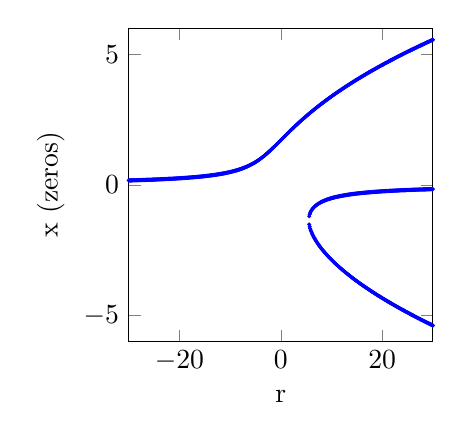
\begin{tikzpicture}

\begin{axis}[%
width=1.520833in,
height=1.565625in,
at={(0.758333in,0.48125in)},
scale only axis,
xmin=-30,
xmax=30,
xlabel={r},
ymin=-6,
ymax=6,
ylabel={x (zeros)}
]
\addplot [color=blue,only marks,mark=*,mark size={0.5},forget plot]
  table[row sep=crcr]{%
-30	0.166512772767465\\
};
\addplot [color=blue,only marks,mark=*,mark size={0.5},forget plot]
  table[row sep=crcr]{%
-29.9	0.167068121576816\\
};
\addplot [color=blue,only marks,mark=*,mark size={0.5},forget plot]
  table[row sep=crcr]{%
-29.8	0.16762717670106\\
};
\addplot [color=blue,only marks,mark=*,mark size={0.5},forget plot]
  table[row sep=crcr]{%
-29.7	0.168189975226301\\
};
\addplot [color=blue,only marks,mark=*,mark size={0.5},forget plot]
  table[row sep=crcr]{%
-29.6	0.168756554732689\\
};
\addplot [color=blue,only marks,mark=*,mark size={0.5},forget plot]
  table[row sep=crcr]{%
-29.5	0.169326953302634\\
};
\addplot [color=blue,only marks,mark=*,mark size={0.5},forget plot]
  table[row sep=crcr]{%
-29.4	0.169901209529164\\
};
\addplot [color=blue,only marks,mark=*,mark size={0.5},forget plot]
  table[row sep=crcr]{%
-29.3	0.170479362524467\\
};
\addplot [color=blue,only marks,mark=*,mark size={0.5},forget plot]
  table[row sep=crcr]{%
-29.2	0.171061451928595\\
};
\addplot [color=blue,only marks,mark=*,mark size={0.5},forget plot]
  table[row sep=crcr]{%
-29.1	0.171647517918344\\
};
\addplot [color=blue,only marks,mark=*,mark size={0.5},forget plot]
  table[row sep=crcr]{%
-29	0.17223760121631\\
};
\addplot [color=blue,only marks,mark=*,mark size={0.5},forget plot]
  table[row sep=crcr]{%
-28.9	0.172831743100136\\
};
\addplot [color=blue,only marks,mark=*,mark size={0.5},forget plot]
  table[row sep=crcr]{%
-28.8	0.173429985411935\\
};
\addplot [color=blue,only marks,mark=*,mark size={0.5},forget plot]
  table[row sep=crcr]{%
-28.7	0.174032370567911\\
};
\addplot [color=blue,only marks,mark=*,mark size={0.5},forget plot]
  table[row sep=crcr]{%
-28.6	0.174638941568175\\
};
\addplot [color=blue,only marks,mark=*,mark size={0.5},forget plot]
  table[row sep=crcr]{%
-28.5	0.175249742006763\\
};
\addplot [color=blue,only marks,mark=*,mark size={0.5},forget plot]
  table[row sep=crcr]{%
-28.4	0.175864816081851\\
};
\addplot [color=blue,only marks,mark=*,mark size={0.5},forget plot]
  table[row sep=crcr]{%
-28.3	0.176484208606195\\
};
\addplot [color=blue,only marks,mark=*,mark size={0.5},forget plot]
  table[row sep=crcr]{%
-28.2	0.177107965017768\\
};
\addplot [color=blue,only marks,mark=*,mark size={0.5},forget plot]
  table[row sep=crcr]{%
-28.1	0.177736131390634\\
};
\addplot [color=blue,only marks,mark=*,mark size={0.5},forget plot]
  table[row sep=crcr]{%
-28	0.178368754446036\\
};
\addplot [color=blue,only marks,mark=*,mark size={0.5},forget plot]
  table[row sep=crcr]{%
-27.9	0.179005881563723\\
};
\addplot [color=blue,only marks,mark=*,mark size={0.5},forget plot]
  table[row sep=crcr]{%
-27.8	0.179647560793504\\
};
\addplot [color=blue,only marks,mark=*,mark size={0.5},forget plot]
  table[row sep=crcr]{%
-27.7	0.180293840867055\\
};
\addplot [color=blue,only marks,mark=*,mark size={0.5},forget plot]
  table[row sep=crcr]{%
-27.6	0.180944771209966\\
};
\addplot [color=blue,only marks,mark=*,mark size={0.5},forget plot]
  table[row sep=crcr]{%
-27.5	0.181600401954048\\
};
\addplot [color=blue,only marks,mark=*,mark size={0.5},forget plot]
  table[row sep=crcr]{%
-27.4	0.182260783949893\\
};
\addplot [color=blue,only marks,mark=*,mark size={0.5},forget plot]
  table[row sep=crcr]{%
-27.3	0.182925968779713\\
};
\addplot [color=blue,only marks,mark=*,mark size={0.5},forget plot]
  table[row sep=crcr]{%
-27.2	0.183596008770435\\
};
\addplot [color=blue,only marks,mark=*,mark size={0.5},forget plot]
  table[row sep=crcr]{%
-27.1	0.184270957007094\\
};
\addplot [color=blue,only marks,mark=*,mark size={0.5},forget plot]
  table[row sep=crcr]{%
-27	0.184950867346501\\
};
\addplot [color=blue,only marks,mark=*,mark size={0.5},forget plot]
  table[row sep=crcr]{%
-26.9	0.185635794431211\\
};
\addplot [color=blue,only marks,mark=*,mark size={0.5},forget plot]
  table[row sep=crcr]{%
-26.8	0.186325793703788\\
};
\addplot [color=blue,only marks,mark=*,mark size={0.5},forget plot]
  table[row sep=crcr]{%
-26.7	0.187020921421381\\
};
\addplot [color=blue,only marks,mark=*,mark size={0.5},forget plot]
  table[row sep=crcr]{%
-26.6	0.187721234670623\\
};
\addplot [color=blue,only marks,mark=*,mark size={0.5},forget plot]
  table[row sep=crcr]{%
-26.5	0.18842679138284\\
};
\addplot [color=blue,only marks,mark=*,mark size={0.5},forget plot]
  table[row sep=crcr]{%
-26.4	0.189137650349609\\
};
\addplot [color=blue,only marks,mark=*,mark size={0.5},forget plot]
  table[row sep=crcr]{%
-26.3	0.189853871238647\\
};
\addplot [color=blue,only marks,mark=*,mark size={0.5},forget plot]
  table[row sep=crcr]{%
-26.2	0.190575514610053\\
};
\addplot [color=blue,only marks,mark=*,mark size={0.5},forget plot]
  table[row sep=crcr]{%
-26.1	0.191302641932909\\
};
\addplot [color=blue,only marks,mark=*,mark size={0.5},forget plot]
  table[row sep=crcr]{%
-26	0.19203531560225\\
};
\addplot [color=blue,only marks,mark=*,mark size={0.5},forget plot]
  table[row sep=crcr]{%
-25.9	0.192773598956408\\
};
\addplot [color=blue,only marks,mark=*,mark size={0.5},forget plot]
  table[row sep=crcr]{%
-25.8	0.19351755629475\\
};
\addplot [color=blue,only marks,mark=*,mark size={0.5},forget plot]
  table[row sep=crcr]{%
-25.7	0.194267252895802\\
};
\addplot [color=blue,only marks,mark=*,mark size={0.5},forget plot]
  table[row sep=crcr]{%
-25.6	0.195022755035796\\
};
\addplot [color=blue,only marks,mark=*,mark size={0.5},forget plot]
  table[row sep=crcr]{%
-25.5	0.195784130007617\\
};
\addplot [color=blue,only marks,mark=*,mark size={0.5},forget plot]
  table[row sep=crcr]{%
-25.4	0.196551446140195\\
};
\addplot [color=blue,only marks,mark=*,mark size={0.5},forget plot]
  table[row sep=crcr]{%
-25.3	0.197324772818328\\
};
\addplot [color=blue,only marks,mark=*,mark size={0.5},forget plot]
  table[row sep=crcr]{%
-25.2	0.198104180502958\\
};
\addplot [color=blue,only marks,mark=*,mark size={0.5},forget plot]
  table[row sep=crcr]{%
-25.1	0.198889740751912\\
};
\addplot [color=blue,only marks,mark=*,mark size={0.5},forget plot]
  table[row sep=crcr]{%
-25	0.199681526241122\\
};
\addplot [color=blue,only marks,mark=*,mark size={0.5},forget plot]
  table[row sep=crcr]{%
-24.9	0.200479610786322\\
};
\addplot [color=blue,only marks,mark=*,mark size={0.5},forget plot]
  table[row sep=crcr]{%
-24.8	0.201284069365261\\
};
\addplot [color=blue,only marks,mark=*,mark size={0.5},forget plot]
  table[row sep=crcr]{%
-24.7	0.20209497814042\\
};
\addplot [color=blue,only marks,mark=*,mark size={0.5},forget plot]
  table[row sep=crcr]{%
-24.6	0.202912414482264\\
};
\addplot [color=blue,only marks,mark=*,mark size={0.5},forget plot]
  table[row sep=crcr]{%
-24.5	0.20373645699303\\
};
\addplot [color=blue,only marks,mark=*,mark size={0.5},forget plot]
  table[row sep=crcr]{%
-24.4	0.204567185531078\\
};
\addplot [color=blue,only marks,mark=*,mark size={0.5},forget plot]
  table[row sep=crcr]{%
-24.3	0.205404681235814\\
};
\addplot [color=blue,only marks,mark=*,mark size={0.5},forget plot]
  table[row sep=crcr]{%
-24.2	0.206249026553196\\
};
\addplot [color=blue,only marks,mark=*,mark size={0.5},forget plot]
  table[row sep=crcr]{%
-24.1	0.207100305261848\\
};
\addplot [color=blue,only marks,mark=*,mark size={0.5},forget plot]
  table[row sep=crcr]{%
-24	0.207958602499793\\
};
\addplot [color=blue,only marks,mark=*,mark size={0.5},forget plot]
  table[row sep=crcr]{%
-23.9	0.208824004791825\\
};
\addplot [color=blue,only marks,mark=*,mark size={0.5},forget plot]
  table[row sep=crcr]{%
-23.8	0.20969660007753\\
};
\addplot [color=blue,only marks,mark=*,mark size={0.5},forget plot]
  table[row sep=crcr]{%
-23.7	0.210576477739986\\
};
\addplot [color=blue,only marks,mark=*,mark size={0.5},forget plot]
  table[row sep=crcr]{%
-23.6	0.211463728635151\\
};
\addplot [color=blue,only marks,mark=*,mark size={0.5},forget plot]
  table[row sep=crcr]{%
-23.5	0.212358445121963\\
};
\addplot [color=blue,only marks,mark=*,mark size={0.5},forget plot]
  table[row sep=crcr]{%
-23.4	0.213260721093167\\
};
\addplot [color=blue,only marks,mark=*,mark size={0.5},forget plot]
  table[row sep=crcr]{%
-23.3	0.214170652006898\\
};
\addplot [color=blue,only marks,mark=*,mark size={0.5},forget plot]
  table[row sep=crcr]{%
-23.2	0.215088334919028\\
};
\addplot [color=blue,only marks,mark=*,mark size={0.5},forget plot]
  table[row sep=crcr]{%
-23.1	0.216013868516315\\
};
\addplot [color=blue,only marks,mark=*,mark size={0.5},forget plot]
  table[row sep=crcr]{%
-23	0.21694735315036\\
};
\addplot [color=blue,only marks,mark=*,mark size={0.5},forget plot]
  table[row sep=crcr]{%
-22.9	0.217888890872407\\
};
\addplot [color=blue,only marks,mark=*,mark size={0.5},forget plot]
  table[row sep=crcr]{%
-22.8	0.218838585469003\\
};
\addplot [color=blue,only marks,mark=*,mark size={0.5},forget plot]
  table[row sep=crcr]{%
-22.7	0.219796542498545\\
};
\addplot [color=blue,only marks,mark=*,mark size={0.5},forget plot]
  table[row sep=crcr]{%
-22.6	0.220762869328741\\
};
\addplot [color=blue,only marks,mark=*,mark size={0.5},forget plot]
  table[row sep=crcr]{%
-22.5	0.221737675175011\\
};
\addplot [color=blue,only marks,mark=*,mark size={0.5},forget plot]
  table[row sep=crcr]{%
-22.4	0.222721071139843\\
};
\addplot [color=blue,only marks,mark=*,mark size={0.5},forget plot]
  table[row sep=crcr]{%
-22.3	0.223713170253158\\
};
\addplot [color=blue,only marks,mark=*,mark size={0.5},forget plot]
  table[row sep=crcr]{%
-22.2	0.224714087513681\\
};
\addplot [color=blue,only marks,mark=*,mark size={0.5},forget plot]
  table[row sep=crcr]{%
-22.1	0.225723939931377\\
};
\addplot [color=blue,only marks,mark=*,mark size={0.5},forget plot]
  table[row sep=crcr]{%
-22	0.226742846570957\\
};
\addplot [color=blue,only marks,mark=*,mark size={0.5},forget plot]
  table[row sep=crcr]{%
-21.9	0.227770928596508\\
};
\addplot [color=blue,only marks,mark=*,mark size={0.5},forget plot]
  table[row sep=crcr]{%
-21.8	0.228808309317261\\
};
\addplot [color=blue,only marks,mark=*,mark size={0.5},forget plot]
  table[row sep=crcr]{%
-21.7	0.229855114234545\\
};
\addplot [color=blue,only marks,mark=*,mark size={0.5},forget plot]
  table[row sep=crcr]{%
-21.6	0.230911471089949\\
};
\addplot [color=blue,only marks,mark=*,mark size={0.5},forget plot]
  table[row sep=crcr]{%
-21.5	0.231977509914745\\
};
\addplot [color=blue,only marks,mark=*,mark size={0.5},forget plot]
  table[row sep=crcr]{%
-21.4	0.233053363080585\\
};
\addplot [color=blue,only marks,mark=*,mark size={0.5},forget plot]
  table[row sep=crcr]{%
-21.3	0.234139165351536\\
};
\addplot [color=blue,only marks,mark=*,mark size={0.5},forget plot]
  table[row sep=crcr]{%
-21.2	0.235235053937473\\
};
\addplot [color=blue,only marks,mark=*,mark size={0.5},forget plot]
  table[row sep=crcr]{%
-21.1	0.236341168548883\\
};
\addplot [color=blue,only marks,mark=*,mark size={0.5},forget plot]
  table[row sep=crcr]{%
-21	0.237457651453117\\
};
\addplot [color=blue,only marks,mark=*,mark size={0.5},forget plot]
  table[row sep=crcr]{%
-20.9	0.238584647532126\\
};
\addplot [color=blue,only marks,mark=*,mark size={0.5},forget plot]
  table[row sep=crcr]{%
-20.8	0.239722304341752\\
};
\addplot [color=blue,only marks,mark=*,mark size={0.5},forget plot]
  table[row sep=crcr]{%
-20.7	0.240870772172585\\
};
\addplot [color=blue,only marks,mark=*,mark size={0.5},forget plot]
  table[row sep=crcr]{%
-20.6	0.242030204112462\\
};
\addplot [color=blue,only marks,mark=*,mark size={0.5},forget plot]
  table[row sep=crcr]{%
-20.5	0.243200756110648\\
};
\addplot [color=blue,only marks,mark=*,mark size={0.5},forget plot]
  table[row sep=crcr]{%
-20.4	0.244382587043743\\
};
\addplot [color=blue,only marks,mark=*,mark size={0.5},forget plot]
  table[row sep=crcr]{%
-20.3	0.24557585878339\\
};
\addplot [color=blue,only marks,mark=*,mark size={0.5},forget plot]
  table[row sep=crcr]{%
-20.2	0.246780736265805\\
};
\addplot [color=blue,only marks,mark=*,mark size={0.5},forget plot]
  table[row sep=crcr]{%
-20.1	0.247997387563227\\
};
\addplot [color=blue,only marks,mark=*,mark size={0.5},forget plot]
  table[row sep=crcr]{%
-20	0.249225983957305\\
};
\addplot [color=blue,only marks,mark=*,mark size={0.5},forget plot]
  table[row sep=crcr]{%
-19.9	0.25046670001452\\
};
\addplot [color=blue,only marks,mark=*,mark size={0.5},forget plot]
  table[row sep=crcr]{%
-19.8	0.251719713663679\\
};
\addplot [color=blue,only marks,mark=*,mark size={0.5},forget plot]
  table[row sep=crcr]{%
-19.7	0.252985206275554\\
};
\addplot [color=blue,only marks,mark=*,mark size={0.5},forget plot]
  table[row sep=crcr]{%
-19.6	0.254263362744742\\
};
\addplot [color=blue,only marks,mark=*,mark size={0.5},forget plot]
  table[row sep=crcr]{%
-19.5	0.255554371573798\\
};
\addplot [color=blue,only marks,mark=*,mark size={0.5},forget plot]
  table[row sep=crcr]{%
-19.4	0.256858424959732\\
};
\addplot [color=blue,only marks,mark=*,mark size={0.5},forget plot]
  table[row sep=crcr]{%
-19.3	0.258175718882928\\
};
\addplot [color=blue,only marks,mark=*,mark size={0.5},forget plot]
  table[row sep=crcr]{%
-19.2	0.259506453198571\\
};
\addplot [color=blue,only marks,mark=*,mark size={0.5},forget plot]
  table[row sep=crcr]{%
-19.1	0.260850831730664\\
};
\addplot [color=blue,only marks,mark=*,mark size={0.5},forget plot]
  table[row sep=crcr]{%
-19	0.262209062368705\\
};
\addplot [color=blue,only marks,mark=*,mark size={0.5},forget plot]
  table[row sep=crcr]{%
-18.9	0.263581357167124\\
};
\addplot [color=blue,only marks,mark=*,mark size={0.5},forget plot]
  table[row sep=crcr]{%
-18.8	0.26496793244756\\
};
\addplot [color=blue,only marks,mark=*,mark size={0.5},forget plot]
  table[row sep=crcr]{%
-18.7	0.266369008904063\\
};
\addplot [color=blue,only marks,mark=*,mark size={0.5},forget plot]
  table[row sep=crcr]{%
-18.6	0.267784811711337\\
};
\addplot [color=blue,only marks,mark=*,mark size={0.5},forget plot]
  table[row sep=crcr]{%
-18.5	0.269215570636094\\
};
\addplot [color=blue,only marks,mark=*,mark size={0.5},forget plot]
  table[row sep=crcr]{%
-18.4	0.270661520151638\\
};
\addplot [color=blue,only marks,mark=*,mark size={0.5},forget plot]
  table[row sep=crcr]{%
-18.3	0.272122899555783\\
};
\addplot [color=blue,only marks,mark=*,mark size={0.5},forget plot]
  table[row sep=crcr]{%
-18.2	0.273599953092205\\
};
\addplot [color=blue,only marks,mark=*,mark size={0.5},forget plot]
  table[row sep=crcr]{%
-18.1	0.27509293007534\\
};
\addplot [color=blue,only marks,mark=*,mark size={0.5},forget plot]
  table[row sep=crcr]{%
-18	0.276602085018959\\
};
\addplot [color=blue,only marks,mark=*,mark size={0.5},forget plot]
  table[row sep=crcr]{%
-17.9	0.278127677768513\\
};
\addplot [color=blue,only marks,mark=*,mark size={0.5},forget plot]
  table[row sep=crcr]{%
-17.8	0.279669973637405\\
};
\addplot [color=blue,only marks,mark=*,mark size={0.5},forget plot]
  table[row sep=crcr]{%
-17.7	0.281229243547282\\
};
\addplot [color=blue,only marks,mark=*,mark size={0.5},forget plot]
  table[row sep=crcr]{%
-17.6	0.282805764172511\\
};
\addplot [color=blue,only marks,mark=*,mark size={0.5},forget plot]
  table[row sep=crcr]{%
-17.5	0.284399818088954\\
};
\addplot [color=blue,only marks,mark=*,mark size={0.5},forget plot]
  table[row sep=crcr]{%
-17.4	0.286011693927199\\
};
\addplot [color=blue,only marks,mark=*,mark size={0.5},forget plot]
  table[row sep=crcr]{%
-17.3	0.28764168653038\\
};
\addplot [color=blue,only marks,mark=*,mark size={0.5},forget plot]
  table[row sep=crcr]{%
-17.2	0.289290097116755\\
};
\addplot [color=blue,only marks,mark=*,mark size={0.5},forget plot]
  table[row sep=crcr]{%
-17.1	0.290957233447179\\
};
\addplot [color=blue,only marks,mark=*,mark size={0.5},forget plot]
  table[row sep=crcr]{%
-17	0.292643409997657\\
};
\addplot [color=blue,only marks,mark=*,mark size={0.5},forget plot]
  table[row sep=crcr]{%
-16.9	0.294348948137125\\
};
\addplot [color=blue,only marks,mark=*,mark size={0.5},forget plot]
  table[row sep=crcr]{%
-16.8	0.296074176310643\\
};
\addplot [color=blue,only marks,mark=*,mark size={0.5},forget plot]
  table[row sep=crcr]{%
-16.7	0.297819430228184\\
};
\addplot [color=blue,only marks,mark=*,mark size={0.5},forget plot]
  table[row sep=crcr]{%
-16.6	0.299585053059193\\
};
\addplot [color=blue,only marks,mark=*,mark size={0.5},forget plot]
  table[row sep=crcr]{%
-16.5	0.301371395633118\\
};
\addplot [color=blue,only marks,mark=*,mark size={0.5},forget plot]
  table[row sep=crcr]{%
-16.4	0.303178816646114\\
};
\addplot [color=blue,only marks,mark=*,mark size={0.5},forget plot]
  table[row sep=crcr]{%
-16.3	0.305007682874104\\
};
\addplot [color=blue,only marks,mark=*,mark size={0.5},forget plot]
  table[row sep=crcr]{%
-16.2	0.30685836939245\\
};
\addplot [color=blue,only marks,mark=*,mark size={0.5},forget plot]
  table[row sep=crcr]{%
-16.1	0.308731259802403\\
};
\addplot [color=blue,only marks,mark=*,mark size={0.5},forget plot]
  table[row sep=crcr]{%
-16	0.310626746464607\\
};
\addplot [color=blue,only marks,mark=*,mark size={0.5},forget plot]
  table[row sep=crcr]{%
-15.9	0.312545230739851\\
};
\addplot [color=blue,only marks,mark=*,mark size={0.5},forget plot]
  table[row sep=crcr]{%
-15.8	0.314487123237342\\
};
\addplot [color=blue,only marks,mark=*,mark size={0.5},forget plot]
  table[row sep=crcr]{%
-15.7	0.316452844070722\\
};
\addplot [color=blue,only marks,mark=*,mark size={0.5},forget plot]
  table[row sep=crcr]{%
-15.6	0.318442823122109\\
};
\addplot [color=blue,only marks,mark=*,mark size={0.5},forget plot]
  table[row sep=crcr]{%
-15.5	0.320457500314412\\
};
\addplot [color=blue,only marks,mark=*,mark size={0.5},forget plot]
  table[row sep=crcr]{%
-15.4	0.322497325892198\\
};
\addplot [color=blue,only marks,mark=*,mark size={0.5},forget plot]
  table[row sep=crcr]{%
-15.3	0.3245627607114\\
};
\addplot [color=blue,only marks,mark=*,mark size={0.5},forget plot]
  table[row sep=crcr]{%
-15.2	0.326654276538141\\
};
\addplot [color=blue,only marks,mark=*,mark size={0.5},forget plot]
  table[row sep=crcr]{%
-15.1	0.328772356356989\\
};
\addplot [color=blue,only marks,mark=*,mark size={0.5},forget plot]
  table[row sep=crcr]{%
-15	0.330917494688949\\
};
\addplot [color=blue,only marks,mark=*,mark size={0.5},forget plot]
  table[row sep=crcr]{%
-14.9	0.333090197919494\\
};
\addplot [color=blue,only marks,mark=*,mark size={0.5},forget plot]
  table[row sep=crcr]{%
-14.8	0.335290984636979\\
};
\addplot [color=blue,only marks,mark=*,mark size={0.5},forget plot]
  table[row sep=crcr]{%
-14.7	0.337520385981769\\
};
\addplot [color=blue,only marks,mark=*,mark size={0.5},forget plot]
  table[row sep=crcr]{%
-14.6	0.339778946006412\\
};
\addplot [color=blue,only marks,mark=*,mark size={0.5},forget plot]
  table[row sep=crcr]{%
-14.5	0.342067222047228\\
};
\addplot [color=blue,only marks,mark=*,mark size={0.5},forget plot]
  table[row sep=crcr]{%
-14.4	0.344385785107664\\
};
\addplot [color=blue,only marks,mark=*,mark size={0.5},forget plot]
  table[row sep=crcr]{%
-14.3	0.34673522025379\\
};
\addplot [color=blue,only marks,mark=*,mark size={0.5},forget plot]
  table[row sep=crcr]{%
-14.2	0.34911612702231\\
};
\addplot [color=blue,only marks,mark=*,mark size={0.5},forget plot]
  table[row sep=crcr]{%
-14.1	0.351529119841489\\
};
\addplot [color=blue,only marks,mark=*,mark size={0.5},forget plot]
  table[row sep=crcr]{%
-14	0.353974828465373\\
};
\addplot [color=blue,only marks,mark=*,mark size={0.5},forget plot]
  table[row sep=crcr]{%
-13.9	0.356453898421724\\
};
\addplot [color=blue,only marks,mark=*,mark size={0.5},forget plot]
  table[row sep=crcr]{%
-13.8	0.358966991474063\\
};
\addplot [color=blue,only marks,mark=*,mark size={0.5},forget plot]
  table[row sep=crcr]{%
-13.7	0.361514786098257\\
};
\addplot [color=blue,only marks,mark=*,mark size={0.5},forget plot]
  table[row sep=crcr]{%
-13.6	0.364097977974063\\
};
\addplot [color=blue,only marks,mark=*,mark size={0.5},forget plot]
  table[row sep=crcr]{%
-13.5	0.366717280492054\\
};
\addplot [color=blue,only marks,mark=*,mark size={0.5},forget plot]
  table[row sep=crcr]{%
-13.4	0.369373425276384\\
};
\addplot [color=blue,only marks,mark=*,mark size={0.5},forget plot]
  table[row sep=crcr]{%
-13.3	0.372067162723797\\
};
\addplot [color=blue,only marks,mark=*,mark size={0.5},forget plot]
  table[row sep=crcr]{%
-13.2	0.374799262559349\\
};
\addplot [color=blue,only marks,mark=*,mark size={0.5},forget plot]
  table[row sep=crcr]{%
-13.1	0.37757051440927\\
};
\addplot [color=blue,only marks,mark=*,mark size={0.5},forget plot]
  table[row sep=crcr]{%
-13	0.38038172839141\\
};
\addplot [color=blue,only marks,mark=*,mark size={0.5},forget plot]
  table[row sep=crcr]{%
-12.9	0.383233735723712\\
};
\addplot [color=blue,only marks,mark=*,mark size={0.5},forget plot]
  table[row sep=crcr]{%
-12.8	0.386127389351138\\
};
\addplot [color=blue,only marks,mark=*,mark size={0.5},forget plot]
  table[row sep=crcr]{%
-12.7	0.389063564591487\\
};
\addplot [color=blue,only marks,mark=*,mark size={0.5},forget plot]
  table[row sep=crcr]{%
-12.6	0.392043159800519\\
};
\addplot [color=blue,only marks,mark=*,mark size={0.5},forget plot]
  table[row sep=crcr]{%
-12.5	0.395067097056796\\
};
\addplot [color=blue,only marks,mark=*,mark size={0.5},forget plot]
  table[row sep=crcr]{%
-12.4	0.398136322866626\\
};
\addplot [color=blue,only marks,mark=*,mark size={0.5},forget plot]
  table[row sep=crcr]{%
-12.3	0.401251808889498\\
};
\addplot [color=blue,only marks,mark=*,mark size={0.5},forget plot]
  table[row sep=crcr]{%
-12.2	0.404414552684345\\
};
\addplot [color=blue,only marks,mark=*,mark size={0.5},forget plot]
  table[row sep=crcr]{%
-12.1	0.407625578476971\\
};
\addplot [color=blue,only marks,mark=*,mark size={0.5},forget plot]
  table[row sep=crcr]{%
-12	0.410885937948929\\
};
\addplot [color=blue,only marks,mark=*,mark size={0.5},forget plot]
  table[row sep=crcr]{%
-11.9	0.414196711048109\\
};
\addplot [color=blue,only marks,mark=*,mark size={0.5},forget plot]
  table[row sep=crcr]{%
-11.8	0.41755900682124\\
};
\addplot [color=blue,only marks,mark=*,mark size={0.5},forget plot]
  table[row sep=crcr]{%
-11.7	0.420973964268475\\
};
\addplot [color=blue,only marks,mark=*,mark size={0.5},forget plot]
  table[row sep=crcr]{%
-11.6	0.424442753220155\\
};
\addplot [color=blue,only marks,mark=*,mark size={0.5},forget plot]
  table[row sep=crcr]{%
-11.5	0.427966575235787\\
};
\addplot [color=blue,only marks,mark=*,mark size={0.5},forget plot]
  table[row sep=crcr]{%
-11.4	0.431546664525193\\
};
\addplot [color=blue,only marks,mark=*,mark size={0.5},forget plot]
  table[row sep=crcr]{%
-11.3	0.435184288891701\\
};
\addplot [color=blue,only marks,mark=*,mark size={0.5},forget plot]
  table[row sep=crcr]{%
-11.2	0.438880750697153\\
};
\addplot [color=blue,only marks,mark=*,mark size={0.5},forget plot]
  table[row sep=crcr]{%
-11.1	0.442637387848389\\
};
\addplot [color=blue,only marks,mark=*,mark size={0.5},forget plot]
  table[row sep=crcr]{%
-11	0.446455574804737\\
};
\addplot [color=blue,only marks,mark=*,mark size={0.5},forget plot]
  table[row sep=crcr]{%
-10.9	0.450336723605914\\
};
\addplot [color=blue,only marks,mark=*,mark size={0.5},forget plot]
  table[row sep=crcr]{%
-10.8	0.454282284919574\\
};
\addplot [color=blue,only marks,mark=*,mark size={0.5},forget plot]
  table[row sep=crcr]{%
-10.7	0.458293749107552\\
};
\addplot [color=blue,only marks,mark=*,mark size={0.5},forget plot]
  table[row sep=crcr]{%
-10.6	0.462372647309702\\
};
\addplot [color=blue,only marks,mark=*,mark size={0.5},forget plot]
  table[row sep=crcr]{%
-10.5	0.466520552543931\\
};
\addplot [color=blue,only marks,mark=*,mark size={0.5},forget plot]
  table[row sep=crcr]{%
-10.4	0.470739080820888\\
};
\addplot [color=blue,only marks,mark=*,mark size={0.5},forget plot]
  table[row sep=crcr]{%
-10.3	0.475029892271404\\
};
\addplot [color=blue,only marks,mark=*,mark size={0.5},forget plot]
  table[row sep=crcr]{%
-10.2	0.479394692284549\\
};
\addplot [color=blue,only marks,mark=*,mark size={0.5},forget plot]
  table[row sep=crcr]{%
-10.1	0.483835232653814\\
};
\addplot [color=blue,only marks,mark=*,mark size={0.5},forget plot]
  table[row sep=crcr]{%
-10	0.488353312728565\\
};
\addplot [color=blue,only marks,mark=*,mark size={0.5},forget plot]
  table[row sep=crcr]{%
-9.9	0.492950780567544\\
};
\addplot [color=blue,only marks,mark=*,mark size={0.5},forget plot]
  table[row sep=crcr]{%
-9.8	0.497629534090708\\
};
\addplot [color=blue,only marks,mark=*,mark size={0.5},forget plot]
  table[row sep=crcr]{%
-9.7	0.502391522225277\\
};
\addplot [color=blue,only marks,mark=*,mark size={0.5},forget plot]
  table[row sep=crcr]{%
-9.6	0.50723874604129\\
};
\addplot [color=blue,only marks,mark=*,mark size={0.5},forget plot]
  table[row sep=crcr]{%
-9.5	0.512173259871415\\
};
\addplot [color=blue,only marks,mark=*,mark size={0.5},forget plot]
  table[row sep=crcr]{%
-9.4	0.517197172409145\\
};
\addplot [color=blue,only marks,mark=*,mark size={0.5},forget plot]
  table[row sep=crcr]{%
-9.3	0.522312647778816\\
};
\addplot [color=blue,only marks,mark=*,mark size={0.5},forget plot]
  table[row sep=crcr]{%
-9.2	0.527521906570149\\
};
\addplot [color=blue,only marks,mark=*,mark size={0.5},forget plot]
  table[row sep=crcr]{%
-9.1	0.532827226829234\\
};
\addplot [color=blue,only marks,mark=*,mark size={0.5},forget plot]
  table[row sep=crcr]{%
-9	0.53823094499699\\
};
\addplot [color=blue,only marks,mark=*,mark size={0.5},forget plot]
  table[row sep=crcr]{%
-8.9	0.543735456785224\\
};
\addplot [color=blue,only marks,mark=*,mark size={0.5},forget plot]
  table[row sep=crcr]{%
-8.8	0.549343217979396\\
};
\addplot [color=blue,only marks,mark=*,mark size={0.5},forget plot]
  table[row sep=crcr]{%
-8.7	0.555056745156131\\
};
\addplot [color=blue,only marks,mark=*,mark size={0.5},forget plot]
  table[row sep=crcr]{%
-8.6	0.56087861630239\\
};
\addplot [color=blue,only marks,mark=*,mark size={0.5},forget plot]
  table[row sep=crcr]{%
-8.5	0.566811471321941\\
};
\addplot [color=blue,only marks,mark=*,mark size={0.5},forget plot]
  table[row sep=crcr]{%
-8.4	0.57285801241355\\
};
\addplot [color=blue,only marks,mark=*,mark size={0.5},forget plot]
  table[row sep=crcr]{%
-8.3	0.579021004303874\\
};
\addplot [color=blue,only marks,mark=*,mark size={0.5},forget plot]
  table[row sep=crcr]{%
-8.2	0.585303274316635\\
};
\addplot [color=blue,only marks,mark=*,mark size={0.5},forget plot]
  table[row sep=crcr]{%
-8.1	0.591707712258148\\
};
\addplot [color=blue,only marks,mark=*,mark size={0.5},forget plot]
  table[row sep=crcr]{%
-8	0.598237270097699\\
};
\addplot [color=blue,only marks,mark=*,mark size={0.5},forget plot]
  table[row sep=crcr]{%
-7.9	0.604894961419646\\
};
\addplot [color=blue,only marks,mark=*,mark size={0.5},forget plot]
  table[row sep=crcr]{%
-7.8	0.611683860622471\\
};
\addplot [color=blue,only marks,mark=*,mark size={0.5},forget plot]
  table[row sep=crcr]{%
-7.7	0.61860710183832\\
};
\addplot [color=blue,only marks,mark=*,mark size={0.5},forget plot]
  table[row sep=crcr]{%
-7.6	0.625667877544859\\
};
\addplot [color=blue,only marks,mark=*,mark size={0.5},forget plot]
  table[row sep=crcr]{%
-7.5	0.6328694368396\\
};
\addplot [color=blue,only marks,mark=*,mark size={0.5},forget plot]
  table[row sep=crcr]{%
-7.4	0.640215083345219\\
};
\addplot [color=blue,only marks,mark=*,mark size={0.5},forget plot]
  table[row sep=crcr]{%
-7.3	0.64770817271278\\
};
\addplot [color=blue,only marks,mark=*,mark size={0.5},forget plot]
  table[row sep=crcr]{%
-7.2	0.655352109688346\\
};
\addplot [color=blue,only marks,mark=*,mark size={0.5},forget plot]
  table[row sep=crcr]{%
-7.1	0.663150344707112\\
};
\addplot [color=blue,only marks,mark=*,mark size={0.5},forget plot]
  table[row sep=crcr]{%
-7	0.671106369978092\\
};
\addplot [color=blue,only marks,mark=*,mark size={0.5},forget plot]
  table[row sep=crcr]{%
-6.9	0.679223715021519\\
};
\addplot [color=blue,only marks,mark=*,mark size={0.5},forget plot]
  table[row sep=crcr]{%
-6.8	0.687505941620572\\
};
\addplot [color=blue,only marks,mark=*,mark size={0.5},forget plot]
  table[row sep=crcr]{%
-6.7	0.695956638148885\\
};
\addplot [color=blue,only marks,mark=*,mark size={0.5},forget plot]
  table[row sep=crcr]{%
-6.6	0.704579413235599\\
};
\addplot [color=blue,only marks,mark=*,mark size={0.5},forget plot]
  table[row sep=crcr]{%
-6.5	0.713377888730588\\
};
\addplot [color=blue,only marks,mark=*,mark size={0.5},forget plot]
  table[row sep=crcr]{%
-6.4	0.722355691933968\\
};
\addplot [color=blue,only marks,mark=*,mark size={0.5},forget plot]
  table[row sep=crcr]{%
-6.3	0.731516447056249\\
};
\addplot [color=blue,only marks,mark=*,mark size={0.5},forget plot]
  table[row sep=crcr]{%
-6.2	0.740863765878569\\
};
\addplot [color=blue,only marks,mark=*,mark size={0.5},forget plot]
  table[row sep=crcr]{%
-6.1	0.750401237586427\\
};
\addplot [color=blue,only marks,mark=*,mark size={0.5},forget plot]
  table[row sep=crcr]{%
-6	0.760132417755419\\
};
\addplot [color=blue,only marks,mark=*,mark size={0.5},forget plot]
  table[row sep=crcr]{%
-5.9	0.77006081647361\\
};
\addplot [color=blue,only marks,mark=*,mark size={0.5},forget plot]
  table[row sep=crcr]{%
-5.8	0.780189885592621\\
};
\addplot [color=blue,only marks,mark=*,mark size={0.5},forget plot]
  table[row sep=crcr]{%
-5.7	0.790523005108164\\
};
\addplot [color=blue,only marks,mark=*,mark size={0.5},forget plot]
  table[row sep=crcr]{%
-5.6	0.801063468680815\\
};
\addplot [color=blue,only marks,mark=*,mark size={0.5},forget plot]
  table[row sep=crcr]{%
-5.5	0.811814468319256\\
};
\addplot [color=blue,only marks,mark=*,mark size={0.5},forget plot]
  table[row sep=crcr]{%
-5.4	0.822779078261001\\
};
\addplot [color=blue,only marks,mark=*,mark size={0.5},forget plot]
  table[row sep=crcr]{%
-5.3	0.833960238099828\\
};
\addplot [color=blue,only marks,mark=*,mark size={0.5},forget plot]
  table[row sep=crcr]{%
-5.2	0.845360735224546\\
};
\addplot [color=blue,only marks,mark=*,mark size={0.5},forget plot]
  table[row sep=crcr]{%
-5.1	0.856983186650342\\
};
\addplot [color=blue,only marks,mark=*,mark size={0.5},forget plot]
  table[row sep=crcr]{%
-5	0.868830020341475\\
};
\addplot [color=blue,only marks,mark=*,mark size={0.5},forget plot]
  table[row sep=crcr]{%
-4.9	0.880903456142354\\
};
\addplot [color=blue,only marks,mark=*,mark size={0.5},forget plot]
  table[row sep=crcr]{%
-4.8	0.89320548645267\\
};
\addplot [color=blue,only marks,mark=*,mark size={0.5},forget plot]
  table[row sep=crcr]{%
-4.7	0.905737856800944\\
};
\addplot [color=blue,only marks,mark=*,mark size={0.5},forget plot]
  table[row sep=crcr]{%
-4.6	0.918502046489043\\
};
\addplot [color=blue,only marks,mark=*,mark size={0.5},forget plot]
  table[row sep=crcr]{%
-4.5	0.93149924949754\\
};
\addplot [color=blue,only marks,mark=*,mark size={0.5},forget plot]
  table[row sep=crcr]{%
-4.4	0.944730355857585\\
};
\addplot [color=blue,only marks,mark=*,mark size={0.5},forget plot]
  table[row sep=crcr]{%
-4.3	0.958195933708624\\
};
\addplot [color=blue,only marks,mark=*,mark size={0.5},forget plot]
  table[row sep=crcr]{%
-4.2	0.971896212272329\\
};
\addplot [color=blue,only marks,mark=*,mark size={0.5},forget plot]
  table[row sep=crcr]{%
-4.1	0.985831065980693\\
};
\addplot [color=blue,only marks,mark=*,mark size={0.5},forget plot]
  table[row sep=crcr]{%
-4	1\\
};
\addplot [color=blue,only marks,mark=*,mark size={0.5},forget plot]
  table[row sep=crcr]{%
-3.9	1.01440213739157\\
};
\addplot [color=blue,only marks,mark=*,mark size={0.5},forget plot]
  table[row sep=crcr]{%
-3.8	1.02903620814449\\
};
\addplot [color=blue,only marks,mark=*,mark size={0.5},forget plot]
  table[row sep=crcr]{%
-3.7	1.04390054030448\\
};
\addplot [color=blue,only marks,mark=*,mark size={0.5},forget plot]
  table[row sep=crcr]{%
-3.6	1.05899305340667\\
};
\addplot [color=blue,only marks,mark=*,mark size={0.5},forget plot]
  table[row sep=crcr]{%
-3.5	1.07431125439768\\
};
\addplot [color=blue,only marks,mark=*,mark size={0.5},forget plot]
  table[row sep=crcr]{%
-3.4	1.08985223620545\\
};
\addplot [color=blue,only marks,mark=*,mark size={0.5},forget plot]
  table[row sep=crcr]{%
-3.3	1.10561267908212\\
};
\addplot [color=blue,only marks,mark=*,mark size={0.5},forget plot]
  table[row sep=crcr]{%
-3.2	1.12158885480881\\
};
\addplot [color=blue,only marks,mark=*,mark size={0.5},forget plot]
  table[row sep=crcr]{%
-3.1	1.13777663380997\\
};
\addplot [color=blue,only marks,mark=*,mark size={0.5},forget plot]
  table[row sep=crcr]{%
-3	1.15417149518144\\
};
\addplot [color=blue,only marks,mark=*,mark size={0.5},forget plot]
  table[row sep=crcr]{%
-2.9	1.1707685395912\\
};
\addplot [color=blue,only marks,mark=*,mark size={0.5},forget plot]
  table[row sep=crcr]{%
-2.8	1.18756250496548\\
};
\addplot [color=blue,only marks,mark=*,mark size={0.5},forget plot]
  table[row sep=crcr]{%
-2.7	1.20454778482799\\
};
\addplot [color=blue,only marks,mark=*,mark size={0.5},forget plot]
  table[row sep=crcr]{%
-2.6	1.22171844911662\\
};
\addplot [color=blue,only marks,mark=*,mark size={0.5},forget plot]
  table[row sep=crcr]{%
-2.5	1.23906826726191\\
};
\addplot [color=blue,only marks,mark=*,mark size={0.5},forget plot]
  table[row sep=crcr]{%
-2.4	1.25659073327606\\
};
\addplot [color=blue,only marks,mark=*,mark size={0.5},forget plot]
  table[row sep=crcr]{%
-2.3	1.27427909257071\\
};
\addplot [color=blue,only marks,mark=*,mark size={0.5},forget plot]
  table[row sep=crcr]{%
-2.2	1.29212637019776\\
};
\addplot [color=blue,only marks,mark=*,mark size={0.5},forget plot]
  table[row sep=crcr]{%
-2.1	1.31012540019011\\
};
\addplot [color=blue,only marks,mark=*,mark size={0.5},forget plot]
  table[row sep=crcr]{%
-2	1.32826885566861\\
};
\addplot [color=blue,only marks,mark=*,mark size={0.5},forget plot]
  table[row sep=crcr]{%
-1.9	1.34654927937896\\
};
\addplot [color=blue,only marks,mark=*,mark size={0.5},forget plot]
  table[row sep=crcr]{%
-1.8	1.36495911432569\\
};
\addplot [color=blue,only marks,mark=*,mark size={0.5},forget plot]
  table[row sep=crcr]{%
-1.7	1.38349073418127\\
};
\addplot [color=blue,only marks,mark=*,mark size={0.5},forget plot]
  table[row sep=crcr]{%
-1.6	1.402136473165\\
};
\addplot [color=blue,only marks,mark=*,mark size={0.5},forget plot]
  table[row sep=crcr]{%
-1.5	1.42088865510817\\
};
\addplot [color=blue,only marks,mark=*,mark size={0.5},forget plot]
  table[row sep=crcr]{%
-1.4	1.43973962144849\\
};
\addplot [color=blue,only marks,mark=*,mark size={0.5},forget plot]
  table[row sep=crcr]{%
-1.3	1.45868175792646\\
};
\addplot [color=blue,only marks,mark=*,mark size={0.5},forget plot]
  table[row sep=crcr]{%
-1.2	1.4777075197886\\
};
\addplot [color=blue,only marks,mark=*,mark size={0.5},forget plot]
  table[row sep=crcr]{%
-1.1	1.49680945533628\\
};
\addplot [color=blue,only marks,mark=*,mark size={0.5},forget plot]
  table[row sep=crcr]{%
-1	1.51598022769282\\
};
\addplot [color=blue,only marks,mark=*,mark size={0.5},forget plot]
  table[row sep=crcr]{%
-0.899999999999999	1.5352126346955\\
};
\addplot [color=blue,only marks,mark=*,mark size={0.5},forget plot]
  table[row sep=crcr]{%
-0.799999999999997	1.55449962685149\\
};
\addplot [color=blue,only marks,mark=*,mark size={0.5},forget plot]
  table[row sep=crcr]{%
-0.699999999999999	1.57383432332773\\
};
\addplot [color=blue,only marks,mark=*,mark size={0.5},forget plot]
  table[row sep=crcr]{%
-0.599999999999998	1.59321002597298\\
};
\addplot [color=blue,only marks,mark=*,mark size={0.5},forget plot]
  table[row sep=crcr]{%
-0.5	1.61262023139589\\
};
\addplot [color=blue,only marks,mark=*,mark size={0.5},forget plot]
  table[row sep=crcr]{%
-0.399999999999999	1.63205864114578\\
};
\addplot [color=blue,only marks,mark=*,mark size={0.5},forget plot]
  table[row sep=crcr]{%
-0.299999999999997	1.65151917006194\\
};
\addplot [color=blue,only marks,mark=*,mark size={0.5},forget plot]
  table[row sep=crcr]{%
-0.199999999999999	1.6709959528736\\
};
\addplot [color=blue,only marks,mark=*,mark size={0.5},forget plot]
  table[row sep=crcr]{%
-0.0999999999999979	1.69048334914588\\
};
\addplot [color=blue,only marks,mark=*,mark size={0.5},forget plot]
  table[row sep=crcr]{%
0	1.7099759466767\\
};
\addplot [color=blue,only marks,mark=*,mark size={0.5},forget plot]
  table[row sep=crcr]{%
0.100000000000001	1.72946856345697\\
};
\addplot [color=blue,only marks,mark=*,mark size={0.5},forget plot]
  table[row sep=crcr]{%
0.200000000000003	1.74895624831096\\
};
\addplot [color=blue,only marks,mark=*,mark size={0.5},forget plot]
  table[row sep=crcr]{%
0.300000000000001	1.76843428033563\\
};
\addplot [color=blue,only marks,mark=*,mark size={0.5},forget plot]
  table[row sep=crcr]{%
0.400000000000002	1.78789816725808\\
};
\addplot [color=blue,only marks,mark=*,mark size={0.5},forget plot]
  table[row sep=crcr]{%
0.5	1.80734364282842\\
};
\addplot [color=blue,only marks,mark=*,mark size={0.5},forget plot]
  table[row sep=crcr]{%
0.600000000000001	1.82676666336239\\
};
\addplot [color=blue,only marks,mark=*,mark size={0.5},forget plot]
  table[row sep=crcr]{%
0.700000000000003	1.84616340354335\\
};
\addplot [color=blue,only marks,mark=*,mark size={0.5},forget plot]
  table[row sep=crcr]{%
0.800000000000001	1.86553025158845\\
};
\addplot [color=blue,only marks,mark=*,mark size={0.5},forget plot]
  table[row sep=crcr]{%
0.900000000000002	1.88486380387726\\
};
\addplot [color=blue,only marks,mark=*,mark size={0.5},forget plot]
  table[row sep=crcr]{%
1	1.90416085913492\\
};
\addplot [color=blue,only marks,mark=*,mark size={0.5},forget plot]
  table[row sep=crcr]{%
1.1	1.92341841225501\\
};
\addplot [color=blue,only marks,mark=*,mark size={0.5},forget plot]
  table[row sep=crcr]{%
1.2	1.94263364784014\\
};
\addplot [color=blue,only marks,mark=*,mark size={0.5},forget plot]
  table[row sep=crcr]{%
1.3	1.96180393353158\\
};
\addplot [color=blue,only marks,mark=*,mark size={0.5},forget plot]
  table[row sep=crcr]{%
1.4	1.98092681319217\\
};
\addplot [color=blue,only marks,mark=*,mark size={0.5},forget plot]
  table[row sep=crcr]{%
1.5	2\\
};
\addplot [color=blue,only marks,mark=*,mark size={0.5},forget plot]
  table[row sep=crcr]{%
1.6	2.01902136950422\\
};
\addplot [color=blue,only marks,mark=*,mark size={0.5},forget plot]
  table[row sep=crcr]{%
1.7	2.03798895268788\\
};
\addplot [color=blue,only marks,mark=*,mark size={0.5},forget plot]
  table[row sep=crcr]{%
1.8	2.05690092907723\\
};
\addplot [color=blue,only marks,mark=*,mark size={0.5},forget plot]
  table[row sep=crcr]{%
1.9	2.07575561993155\\
};
\addplot [color=blue,only marks,mark=*,mark size={0.5},forget plot]
  table[row sep=crcr]{%
2	2.09455148154233\\
};
\addplot [color=blue,only marks,mark=*,mark size={0.5},forget plot]
  table[row sep=crcr]{%
2.1	2.11328709866663\\
};
\addplot [color=blue,only marks,mark=*,mark size={0.5},forget plot]
  table[row sep=crcr]{%
2.2	2.13196117811472\\
};
\addplot [color=blue,only marks,mark=*,mark size={0.5},forget plot]
  table[row sep=crcr]{%
2.3	2.1505725425088\\
};
\addplot [color=blue,only marks,mark=*,mark size={0.5},forget plot]
  table[row sep=crcr]{%
2.4	2.16912012422595\\
};
\addplot [color=blue,only marks,mark=*,mark size={0.5},forget plot]
  table[row sep=crcr]{%
2.5	2.18760295953562\\
};
\addplot [color=blue,only marks,mark=*,mark size={0.5},forget plot]
  table[row sep=crcr]{%
2.6	2.20602018293923\\
};
\addplot [color=blue,only marks,mark=*,mark size={0.5},forget plot]
  table[row sep=crcr]{%
2.7	2.22437102171702\\
};
\addplot [color=blue,only marks,mark=*,mark size={0.5},forget plot]
  table[row sep=crcr]{%
2.8	2.24265479068539\\
};
\addplot [color=blue,only marks,mark=*,mark size={0.5},forget plot]
  table[row sep=crcr]{%
2.9	2.26087088716602\\
};
\addplot [color=blue,only marks,mark=*,mark size={0.5},forget plot]
  table[row sep=crcr]{%
3	2.27901878616659\\
};
\addplot [color=blue,only marks,mark=*,mark size={0.5},forget plot]
  table[row sep=crcr]{%
3.1	2.29709803577162\\
};
\addplot [color=blue,only marks,mark=*,mark size={0.5},forget plot]
  table[row sep=crcr]{%
3.2	2.31510825274071\\
};
\addplot [color=blue,only marks,mark=*,mark size={0.5},forget plot]
  table[row sep=crcr]{%
3.3	2.33304911831073\\
};
\addplot [color=blue,only marks,mark=*,mark size={0.5},forget plot]
  table[row sep=crcr]{%
3.4	2.35092037419748\\
};
\addplot [color=blue,only marks,mark=*,mark size={0.5},forget plot]
  table[row sep=crcr]{%
3.5	2.36872181879195\\
};
\addplot [color=blue,only marks,mark=*,mark size={0.5},forget plot]
  table[row sep=crcr]{%
3.6	2.38645330354561\\
};
\addplot [color=blue,only marks,mark=*,mark size={0.5},forget plot]
  table[row sep=crcr]{%
3.7	2.40411472953899\\
};
\addplot [color=blue,only marks,mark=*,mark size={0.5},forget plot]
  table[row sep=crcr]{%
3.8	2.42170604422722\\
};
\addplot [color=blue,only marks,mark=*,mark size={0.5},forget plot]
  table[row sep=crcr]{%
3.9	2.43922723835641\\
};
\addplot [color=blue,only marks,mark=*,mark size={0.5},forget plot]
  table[row sep=crcr]{%
4	2.45667834304411\\
};
\addplot [color=blue,only marks,mark=*,mark size={0.5},forget plot]
  table[row sep=crcr]{%
4.1	2.47405942701757\\
};
\addplot [color=blue,only marks,mark=*,mark size={0.5},forget plot]
  table[row sep=crcr]{%
4.2	2.49137059400302\\
};
\addplot [color=blue,only marks,mark=*,mark size={0.5},forget plot]
  table[row sep=crcr]{%
4.3	2.50861198025967\\
};
\addplot [color=blue,only marks,mark=*,mark size={0.5},forget plot]
  table[row sep=crcr]{%
4.4	2.52578375225169\\
};
\addplot [color=blue,only marks,mark=*,mark size={0.5},forget plot]
  table[row sep=crcr]{%
4.5	2.54288610445218\\
};
\addplot [color=blue,only marks,mark=*,mark size={0.5},forget plot]
  table[row sep=crcr]{%
4.6	2.55991925727263\\
};
\addplot [color=blue,only marks,mark=*,mark size={0.5},forget plot]
  table[row sep=crcr]{%
4.7	2.57688345511197\\
};
\addplot [color=blue,only marks,mark=*,mark size={0.5},forget plot]
  table[row sep=crcr]{%
4.8	2.59377896451931\\
};
\addplot [color=blue,only marks,mark=*,mark size={0.5},forget plot]
  table[row sep=crcr]{%
4.9	2.6106060724646\\
};
\addplot [color=blue,only marks,mark=*,mark size={0.5},forget plot]
  table[row sep=crcr]{%
5	2.62736508471183\\
};
\addplot [color=blue,only marks,mark=*,mark size={0.5},forget plot]
  table[row sep=crcr]{%
5.1	2.64405632428936\\
};
\addplot [color=blue,only marks,mark=*,mark size={0.5},forget plot]
  table[row sep=crcr]{%
5.2	2.66068013005228\\
};
\addplot [color=blue,only marks,mark=*,mark size={0.5},forget plot]
  table[row sep=crcr]{%
5.3	2.677236855332\\
};
\addplot [color=blue,only marks,mark=*,mark size={0.5},forget plot]
  table[row sep=crcr]{%
5.4	2.69372686666831\\
};
\addplot [color=blue,only marks,mark=*,mark size={0.5},forget plot]
  table[row sep=crcr]{%
5.5	2.71015054261934\\
};
\addplot [color=blue,only marks,mark=*,mark size={0.5},forget plot]
  table[row sep=crcr]{%
5.6	2.72650827264537\\
};
\addplot [color=blue,only marks,mark=*,mark size={0.5},forget plot]
  table[row sep=crcr]{%
5.6	-1.5201441595787\\
};
\addplot [color=blue,only marks,mark=*,mark size={0.5},forget plot]
  table[row sep=crcr]{%
5.6	-1.20636411306668\\
};
\addplot [color=blue,only marks,mark=*,mark size={0.5},forget plot]
  table[row sep=crcr]{%
5.7	2.74280045606214\\
};
\addplot [color=blue,only marks,mark=*,mark size={0.5},forget plot]
  table[row sep=crcr]{%
5.7	-1.61178376255247\\
};
\addplot [color=blue,only marks,mark=*,mark size={0.5},forget plot]
  table[row sep=crcr]{%
5.7	-1.13101669350966\\
};
\addplot [color=blue,only marks,mark=*,mark size={0.5},forget plot]
  table[row sep=crcr]{%
5.8	2.75902750105995\\
};
\addplot [color=blue,only marks,mark=*,mark size={0.5},forget plot]
  table[row sep=crcr]{%
5.8	-1.68088633769772\\
};
\addplot [color=blue,only marks,mark=*,mark size={0.5},forget plot]
  table[row sep=crcr]{%
5.8	-1.07814116336223\\
};
\addplot [color=blue,only marks,mark=*,mark size={0.5},forget plot]
  table[row sep=crcr]{%
5.9	2.77518982378478\\
};
\addplot [color=blue,only marks,mark=*,mark size={0.5},forget plot]
  table[row sep=crcr]{%
5.9	-1.73936341740566\\
};
\addplot [color=blue,only marks,mark=*,mark size={0.5},forget plot]
  table[row sep=crcr]{%
5.9	-1.03582640637912\\
};
\addplot [color=blue,only marks,mark=*,mark size={0.5},forget plot]
  table[row sep=crcr]{%
6	2.79128784747792\\
};
\addplot [color=blue,only marks,mark=*,mark size={0.5},forget plot]
  table[row sep=crcr]{%
6	-1.79128784747792\\
};
\addplot [color=blue,only marks,mark=*,mark size={0.5},forget plot]
  table[row sep=crcr]{%
6	-1\\
};
\addplot [color=blue,only marks,mark=*,mark size={0.5},forget plot]
  table[row sep=crcr]{%
6.1	2.80732200167071\\
};
\addplot [color=blue,only marks,mark=*,mark size={0.5},forget plot]
  table[row sep=crcr]{%
6.1	-1.83864075232001\\
};
\addplot [color=blue,only marks,mark=*,mark size={0.5},forget plot]
  table[row sep=crcr]{%
6.1	-0.968681249350711\\
};
\addplot [color=blue,only marks,mark=*,mark size={0.5},forget plot]
  table[row sep=crcr]{%
6.2	2.82329272143138\\
};
\addplot [color=blue,only marks,mark=*,mark size={0.5},forget plot]
  table[row sep=crcr]{%
6.2	-1.88256424828679\\
};
\addplot [color=blue,only marks,mark=*,mark size={0.5},forget plot]
  table[row sep=crcr]{%
6.2	-0.940728473144592\\
};
\addplot [color=blue,only marks,mark=*,mark size={0.5},forget plot]
  table[row sep=crcr]{%
6.3	2.83920044666076\\
};
\addplot [color=blue,only marks,mark=*,mark size={0.5},forget plot]
  table[row sep=crcr]{%
6.3	-1.92378830109601\\
};
\addplot [color=blue,only marks,mark=*,mark size={0.5},forget plot]
  table[row sep=crcr]{%
6.3	-0.915412145564753\\
};
\addplot [color=blue,only marks,mark=*,mark size={0.5},forget plot]
  table[row sep=crcr]{%
6.4	2.85504562143421\\
};
\addplot [color=blue,only marks,mark=*,mark size={0.5},forget plot]
  table[row sep=crcr]{%
6.4	-1.96281326892368\\
};
\addplot [color=blue,only marks,mark=*,mark size={0.5},forget plot]
  table[row sep=crcr]{%
6.4	-0.892232352510536\\
};
\addplot [color=blue,only marks,mark=*,mark size={0.5},forget plot]
  table[row sep=crcr]{%
6.5	2.87082869338697\\
};
\addplot [color=blue,only marks,mark=*,mark size={0.5},forget plot]
  table[row sep=crcr]{%
6.5	-2\\
};
\addplot [color=blue,only marks,mark=*,mark size={0.5},forget plot]
  table[row sep=crcr]{%
6.5	-0.87082869338697\\
};
\addplot [color=blue,only marks,mark=*,mark size={0.5},forget plot]
  table[row sep=crcr]{%
6.6	2.88655011314039\\
};
\addplot [color=blue,only marks,mark=*,mark size={0.5},forget plot]
  table[row sep=crcr]{%
6.6	-2.03561898812257\\
};
\addplot [color=blue,only marks,mark=*,mark size={0.5},forget plot]
  table[row sep=crcr]{%
6.6	-0.850931125017815\\
};
\addplot [color=blue,only marks,mark=*,mark size={0.5},forget plot]
  table[row sep=crcr]{%
6.7	2.90221033376663\\
};
\addplot [color=blue,only marks,mark=*,mark size={0.5},forget plot]
  table[row sep=crcr]{%
6.7	-2.06987926454226\\
};
\addplot [color=blue,only marks,mark=*,mark size={0.5},forget plot]
  table[row sep=crcr]{%
6.7	-0.832331069224363\\
};
\addplot [color=blue,only marks,mark=*,mark size={0.5},forget plot]
  table[row sep=crcr]{%
6.8	2.91780981028963\\
};
\addplot [color=blue,only marks,mark=*,mark size={0.5},forget plot]
  table[row sep=crcr]{%
6.8	-2.10294638923821\\
};
\addplot [color=blue,only marks,mark=*,mark size={0.5},forget plot]
  table[row sep=crcr]{%
6.8	-0.814863421051419\\
};
\addplot [color=blue,only marks,mark=*,mark size={0.5},forget plot]
  table[row sep=crcr]{%
6.9	2.93334899922001\\
};
\addplot [color=blue,only marks,mark=*,mark size={0.5},forget plot]
  table[row sep=crcr]{%
6.9	-2.13495418400961\\
};
\addplot [color=blue,only marks,mark=*,mark size={0.5},forget plot]
  table[row sep=crcr]{%
6.9	-0.798394815210392\\
};
\addplot [color=blue,only marks,mark=*,mark size={0.5},forget plot]
  table[row sep=crcr]{%
7	2.94882835812209\\
};
\addplot [color=blue,only marks,mark=*,mark size={0.5},forget plot]
  table[row sep=crcr]{%
7	-2.16601267945794\\
};
\addplot [color=blue,only marks,mark=*,mark size={0.5},forget plot]
  table[row sep=crcr]{%
7	-0.782815678664154\\
};
\addplot [color=blue,only marks,mark=*,mark size={0.5},forget plot]
  table[row sep=crcr]{%
7.1	2.96424834521096\\
};
\addplot [color=blue,only marks,mark=*,mark size={0.5},forget plot]
  table[row sep=crcr]{%
7.1	-2.19621367045262\\
};
\addplot [color=blue,only marks,mark=*,mark size={0.5},forget plot]
  table[row sep=crcr]{%
7.1	-0.768034674758341\\
};
\addplot [color=blue,only marks,mark=*,mark size={0.5},forget plot]
  table[row sep=crcr]{%
7.2	2.97960941897779\\
};
\addplot [color=blue,only marks,mark=*,mark size={0.5},forget plot]
  table[row sep=crcr]{%
7.2	-2.22563470531275\\
};
\addplot [color=blue,only marks,mark=*,mark size={0.5},forget plot]
  table[row sep=crcr]{%
7.2	-0.753974713665039\\
};
\addplot [color=blue,only marks,mark=*,mark size={0.5},forget plot]
  table[row sep=crcr]{%
7.3	2.99491203784181\\
};
\addplot [color=blue,only marks,mark=*,mark size={0.5},forget plot]
  table[row sep=crcr]{%
7.3	-2.25434201706903\\
};
\addplot [color=blue,only marks,mark=*,mark size={0.5},forget plot]
  table[row sep=crcr]{%
7.3	-0.740570020772782\\
};
\addplot [color=blue,only marks,mark=*,mark size={0.5},forget plot]
  table[row sep=crcr]{%
7.4	3.01015665982716\\
};
\addplot [color=blue,only marks,mark=*,mark size={0.5},forget plot]
  table[row sep=crcr]{%
7.4	-2.28239272092512\\
};
\addplot [color=blue,only marks,mark=*,mark size={0.5},forget plot]
  table[row sep=crcr]{%
7.4	-0.727763938902037\\
};
\addplot [color=blue,only marks,mark=*,mark size={0.5},forget plot]
  table[row sep=crcr]{%
7.5	3.02534374226326\\
};
\addplot [color=blue,only marks,mark=*,mark size={0.5},forget plot]
  table[row sep=crcr]{%
7.5	-2.30983649080651\\
};
\addplot [color=blue,only marks,mark=*,mark size={0.5},forget plot]
  table[row sep=crcr]{%
7.5	-0.715507251456748\\
};
\addplot [color=blue,only marks,mark=*,mark size={0.5},forget plot]
  table[row sep=crcr]{%
7.6	3.04047374150713\\
};
\addplot [color=blue,only marks,mark=*,mark size={0.5},forget plot]
  table[row sep=crcr]{%
7.6	-2.33671685850844\\
};
\addplot [color=blue,only marks,mark=*,mark size={0.5},forget plot]
  table[row sep=crcr]{%
7.6	-0.703756882998695\\
};
\addplot [color=blue,only marks,mark=*,mark size={0.5},forget plot]
  table[row sep=crcr]{%
7.7	3.05554711268645\\
};
\addplot [color=blue,only marks,mark=*,mark size={0.5},forget plot]
  table[row sep=crcr]{%
7.7	-2.36307223443096\\
};
\addplot [color=blue,only marks,mark=*,mark size={0.5},forget plot]
  table[row sep=crcr]{%
7.7	-0.692474878255498\\
};
\addplot [color=blue,only marks,mark=*,mark size={0.5},forget plot]
  table[row sep=crcr]{%
7.8	3.07056430946193\\
};
\addplot [color=blue,only marks,mark=*,mark size={0.5},forget plot]
  table[row sep=crcr]{%
7.8	-2.3889367195837\\
};
\addplot [color=blue,only marks,mark=*,mark size={0.5},forget plot]
  table[row sep=crcr]{%
7.8	-0.681627589878234\\
};
\addplot [color=blue,only marks,mark=*,mark size={0.5},forget plot]
  table[row sep=crcr]{%
7.9	3.08552578380798\\
};
\addplot [color=blue,only marks,mark=*,mark size={0.5},forget plot]
  table[row sep=crcr]{%
7.9	-2.41434075881669\\
};
\addplot [color=blue,only marks,mark=*,mark size={0.5},forget plot]
  table[row sep=crcr]{%
7.9	-0.671185024991289\\
};
\addplot [color=blue,only marks,mark=*,mark size={0.5},forget plot]
  table[row sep=crcr]{%
8	3.10043198581039\\
};
\addplot [color=blue,only marks,mark=*,mark size={0.5},forget plot]
  table[row sep=crcr]{%
8	-2.43931167168388\\
};
\addplot [color=blue,only marks,mark=*,mark size={0.5},forget plot]
  table[row sep=crcr]{%
8	-0.661120314126504\\
};
\addplot [color=blue,only marks,mark=*,mark size={0.5},forget plot]
  table[row sep=crcr]{%
8.1	3.11528336348001\\
};
\addplot [color=blue,only marks,mark=*,mark size={0.5},forget plot]
  table[row sep=crcr]{%
8.1	-2.4638740878691\\
};
\addplot [color=blue,only marks,mark=*,mark size={0.5},forget plot]
  table[row sep=crcr]{%
8.1	-0.651409275610905\\
};
\addplot [color=blue,only marks,mark=*,mark size={0.5},forget plot]
  table[row sep=crcr]{%
8.2	3.13008036258158\\
};
\addplot [color=blue,only marks,mark=*,mark size={0.5},forget plot]
  table[row sep=crcr]{%
8.2	-2.48805030736518\\
};
\addplot [color=blue,only marks,mark=*,mark size={0.5},forget plot]
  table[row sep=crcr]{%
8.2	-0.642030055216396\\
};
\addplot [color=blue,only marks,mark=*,mark size={0.5},forget plot]
  table[row sep=crcr]{%
8.3	3.1448234264765\\
};
\addplot [color=blue,only marks,mark=*,mark size={0.5},forget plot]
  table[row sep=crcr]{%
8.3	-2.51186060073212\\
};
\addplot [color=blue,only marks,mark=*,mark size={0.5},forget plot]
  table[row sep=crcr]{%
8.3	-0.632962825744371\\
};
\addplot [color=blue,only marks,mark=*,mark size={0.5},forget plot]
  table[row sep=crcr]{%
8.40000000000001	3.15951299597882\\
};
\addplot [color=blue,only marks,mark=*,mark size={0.5},forget plot]
  table[row sep=crcr]{%
8.40000000000001	-2.53532346120063\\
};
\addplot [color=blue,only marks,mark=*,mark size={0.5},forget plot]
  table[row sep=crcr]{%
8.40000000000001	-0.624189534778197\\
};
\addplot [color=blue,only marks,mark=*,mark size={0.5},forget plot]
  table[row sep=crcr]{%
8.5	3.17414950922372\\
};
\addplot [color=blue,only marks,mark=*,mark size={0.5},forget plot]
  table[row sep=crcr]{%
8.5	-2.55845581774883\\
};
\addplot [color=blue,only marks,mark=*,mark size={0.5},forget plot]
  table[row sep=crcr]{%
8.5	-0.615693691474893\\
};
\addplot [color=blue,only marks,mark=*,mark size={0.5},forget plot]
  table[row sep=crcr]{%
8.6	3.18873340154742\\
};
\addplot [color=blue,only marks,mark=*,mark size={0.5},forget plot]
  table[row sep=crcr]{%
8.6	-2.58127321630183\\
};
\addplot [color=blue,only marks,mark=*,mark size={0.5},forget plot]
  table[row sep=crcr]{%
8.6	-0.607460185245596\\
};
\addplot [color=blue,only marks,mark=*,mark size={0.5},forget plot]
  table[row sep=crcr]{%
8.7	3.20326510537806\\
};
\addplot [color=blue,only marks,mark=*,mark size={0.5},forget plot]
  table[row sep=crcr]{%
8.7	-2.60378997470438\\
};
\addplot [color=blue,only marks,mark=*,mark size={0.5},forget plot]
  table[row sep=crcr]{%
8.7	-0.599475130673682\\
};
\addplot [color=blue,only marks,mark=*,mark size={0.5},forget plot]
  table[row sep=crcr]{%
8.8	3.21774505013668\\
};
\addplot [color=blue,only marks,mark=*,mark size={0.5},forget plot]
  table[row sep=crcr]{%
8.8	-2.62601931596957\\
};
\addplot [color=blue,only marks,mark=*,mark size={0.5},forget plot]
  table[row sep=crcr]{%
8.8	-0.591725734167116\\
};
\addplot [color=blue,only marks,mark=*,mark size={0.5},forget plot]
  table[row sep=crcr]{%
8.90000000000001	3.23217366214775\\
};
\addplot [color=blue,only marks,mark=*,mark size={0.5},forget plot]
  table[row sep=crcr]{%
8.90000000000001	-2.64797348341938\\
};
\addplot [color=blue,only marks,mark=*,mark size={0.5},forget plot]
  table[row sep=crcr]{%
8.90000000000001	-0.584200178728368\\
};
\addplot [color=blue,only marks,mark=*,mark size={0.5},forget plot]
  table[row sep=crcr]{%
9	3.24655136455856\\
};
\addplot [color=blue,only marks,mark=*,mark size={0.5},forget plot]
  table[row sep=crcr]{%
9	-2.66966384064223\\
};
\addplot [color=blue,only marks,mark=*,mark size={0.5},forget plot]
  table[row sep=crcr]{%
9	-0.57688752391634\\
};
\addplot [color=blue,only marks,mark=*,mark size={0.5},forget plot]
  table[row sep=crcr]{%
9.1	3.26087857726703\\
};
\addplot [color=blue,only marks,mark=*,mark size={0.5},forget plot]
  table[row sep=crcr]{%
9.1	-2.69110095864932\\
};
\addplot [color=blue,only marks,mark=*,mark size={0.5},forget plot]
  table[row sep=crcr]{%
9.1	-0.569777618617707\\
};
\addplot [color=blue,only marks,mark=*,mark size={0.5},forget plot]
  table[row sep=crcr]{%
9.2	3.27515571685716\\
};
\addplot [color=blue,only marks,mark=*,mark size={0.5},forget plot]
  table[row sep=crcr]{%
9.2	-2.71229469218221\\
};
\addplot [color=blue,only marks,mark=*,mark size={0.5},forget plot]
  table[row sep=crcr]{%
9.2	-0.562861024674943\\
};
\addplot [color=blue,only marks,mark=*,mark size={0.5},forget plot]
  table[row sep=crcr]{%
9.3	3.28938319654189\\
};
\addplot [color=blue,only marks,mark=*,mark size={0.5},forget plot]
  table[row sep=crcr]{%
9.3	-2.73325424678085\\
};
\addplot [color=blue,only marks,mark=*,mark size={0.5},forget plot]
  table[row sep=crcr]{%
9.3	-0.556128949761043\\
};
\addplot [color=blue,only marks,mark=*,mark size={0.5},forget plot]
  table[row sep=crcr]{%
9.40000000000001	3.30356142611275\\
};
\addplot [color=blue,only marks,mark=*,mark size={0.5},forget plot]
  table[row sep=crcr]{%
9.40000000000001	-2.75398823794672\\
};
\addplot [color=blue,only marks,mark=*,mark size={0.5},forget plot]
  table[row sep=crcr]{%
9.40000000000001	-0.54957318816603\\
};
\addplot [color=blue,only marks,mark=*,mark size={0.5},forget plot]
  table[row sep=crcr]{%
9.5	3.31769081189579\\
};
\addplot [color=blue,only marks,mark=*,mark size={0.5},forget plot]
  table[row sep=crcr]{%
9.5	-2.77450474351322\\
};
\addplot [color=blue,only marks,mark=*,mark size={0.5},forget plot]
  table[row sep=crcr]{%
9.5	-0.543186068382565\\
};
\addplot [color=blue,only marks,mark=*,mark size={0.5},forget plot]
  table[row sep=crcr]{%
9.6	3.33177175671348\\
};
\addplot [color=blue,only marks,mark=*,mark size={0.5},forget plot]
  table[row sep=crcr]{%
9.6	-2.79481135015493\\
};
\addplot [color=blue,only marks,mark=*,mark size={0.5},forget plot]
  table[row sep=crcr]{%
9.6	-0.536960406558547\\
};
\addplot [color=blue,only marks,mark=*,mark size={0.5},forget plot]
  table[row sep=crcr]{%
9.7	3.34580465985222\\
};
\addplot [color=blue,only marks,mark=*,mark size={0.5},forget plot]
  table[row sep=crcr]{%
9.7	-2.8149151948201\\
};
\addplot [color=blue,only marks,mark=*,mark size={0.5},forget plot]
  table[row sep=crcr]{%
9.7	-0.53088946503213\\
};
\addplot [color=blue,only marks,mark=*,mark size={0.5},forget plot]
  table[row sep=crcr]{%
9.8	3.35978991703492\\
};
\addplot [color=blue,only marks,mark=*,mark size={0.5},forget plot]
  table[row sep=crcr]{%
9.8	-2.83482300174911\\
};
\addplot [color=blue,only marks,mark=*,mark size={0.5},forget plot]
  table[row sep=crcr]{%
9.8	-0.524966915285807\\
};
\addplot [color=blue,only marks,mark=*,mark size={0.5},forget plot]
  table[row sep=crcr]{%
9.90000000000001	3.37372792039841\\
};
\addplot [color=blue,only marks,mark=*,mark size={0.5},forget plot]
  table[row sep=crcr]{%
9.90000000000001	-2.85454111564209\\
};
\addplot [color=blue,only marks,mark=*,mark size={0.5},forget plot]
  table[row sep=crcr]{%
9.90000000000001	-0.519186804756314\\
};
\addplot [color=blue,only marks,mark=*,mark size={0.5},forget plot]
  table[row sep=crcr]{%
10	3.38761905847542\\
};
\addplot [color=blue,only marks,mark=*,mark size={0.5},forget plot]
  table[row sep=crcr]{%
10	-2.87407553145526\\
};
\addplot [color=blue,only marks,mark=*,mark size={0.5},forget plot]
  table[row sep=crcr]{%
10	-0.513543527020155\\
};
\addplot [color=blue,only marks,mark=*,mark size={0.5},forget plot]
  table[row sep=crcr]{%
10.1	3.40146371618065\\
};
\addplot [color=blue,only marks,mark=*,mark size={0.5},forget plot]
  table[row sep=crcr]{%
10.1	-2.89343192123691\\
};
\addplot [color=blue,only marks,mark=*,mark size={0.5},forget plot]
  table[row sep=crcr]{%
10.1	-0.508031794943738\\
};
\addplot [color=blue,only marks,mark=*,mark size={0.5},forget plot]
  table[row sep=crcr]{%
10.2	3.4152622748008\\
};
\addplot [color=blue,only marks,mark=*,mark size={0.5},forget plot]
  table[row sep=crcr]{%
10.2	-2.91261565835569\\
};
\addplot [color=blue,only marks,mark=*,mark size={0.5},forget plot]
  table[row sep=crcr]{%
10.2	-0.502646616445116\\
};
\addplot [color=blue,only marks,mark=*,mark size={0.5},forget plot]
  table[row sep=crcr]{%
10.3	3.42901511198815\\
};
\addplot [color=blue,only marks,mark=*,mark size={0.5},forget plot]
  table[row sep=crcr]{%
10.3	-2.93163183942518\\
};
\addplot [color=blue,only marks,mark=*,mark size={0.5},forget plot]
  table[row sep=crcr]{%
10.3	-0.497383272562963\\
};
\addplot [color=blue,only marks,mark=*,mark size={0.5},forget plot]
  table[row sep=crcr]{%
10.4	3.44272260175755\\
};
\addplot [color=blue,only marks,mark=*,mark size={0.5},forget plot]
  table[row sep=crcr]{%
10.4	-2.95048530418796\\
};
\addplot [color=blue,only marks,mark=*,mark size={0.5},forget plot]
  table[row sep=crcr]{%
10.4	-0.492237297569594\\
};
\addplot [color=blue,only marks,mark=*,mark size={0.5},forget plot]
  table[row sep=crcr]{%
10.5	3.45638511448658\\
};
\addplot [color=blue,only marks,mark=*,mark size={0.5},forget plot]
  table[row sep=crcr]{%
10.5	-2.96918065358697\\
};
\addplot [color=blue,only marks,mark=*,mark size={0.5},forget plot]
  table[row sep=crcr]{%
10.5	-0.487204460899606\\
};
\addplot [color=blue,only marks,mark=*,mark size={0.5},forget plot]
  table[row sep=crcr]{%
10.6	3.47000301691848\\
};
\addplot [color=blue,only marks,mark=*,mark size={0.5},forget plot]
  table[row sep=crcr]{%
10.6	-2.98772226622311\\
};
\addplot [color=blue,only marks,mark=*,mark size={0.5},forget plot]
  table[row sep=crcr]{%
10.6	-0.482280750695366\\
};
\addplot [color=blue,only marks,mark=*,mark size={0.5},forget plot]
  table[row sep=crcr]{%
10.7	3.48357667216792\\
};
\addplot [color=blue,only marks,mark=*,mark size={0.5},forget plot]
  table[row sep=crcr]{%
10.7	-3.0061143133721\\
};
\addplot [color=blue,only marks,mark=*,mark size={0.5},forget plot]
  table[row sep=crcr]{%
10.7	-0.477462358795809\\
};
\addplot [color=blue,only marks,mark=*,mark size={0.5},forget plot]
  table[row sep=crcr]{%
10.8	3.49710643972913\\
};
\addplot [color=blue,only marks,mark=*,mark size={0.5},forget plot]
  table[row sep=crcr]{%
10.8	-3.02436077271248\\
};
\addplot [color=blue,only marks,mark=*,mark size={0.5},forget plot]
  table[row sep=crcr]{%
10.8	-0.472745667016652\\
};
\addplot [color=blue,only marks,mark=*,mark size={0.5},forget plot]
  table[row sep=crcr]{%
10.9	3.51059267548644\\
};
\addplot [color=blue,only marks,mark=*,mark size={0.5},forget plot]
  table[row sep=crcr]{%
10.9	-3.04246544089777\\
};
\addplot [color=blue,only marks,mark=*,mark size={0.5},forget plot]
  table[row sep=crcr]{%
10.9	-0.468127234588675\\
};
\addplot [color=blue,only marks,mark=*,mark size={0.5},forget plot]
  table[row sep=crcr]{%
11	3.52403573172689\\
};
\addplot [color=blue,only marks,mark=*,mark size={0.5},forget plot]
  table[row sep=crcr]{%
11	-3.06043194509014\\
};
\addplot [color=blue,only marks,mark=*,mark size={0.5},forget plot]
  table[row sep=crcr]{%
11	-0.463603786636745\\
};
\addplot [color=blue,only marks,mark=*,mark size={0.5},forget plot]
  table[row sep=crcr]{%
11.1	3.53743595715476\\
};
\addplot [color=blue,only marks,mark=*,mark size={0.5},forget plot]
  table[row sep=crcr]{%
11.1	-3.07826375355871\\
};
\addplot [color=blue,only marks,mark=*,mark size={0.5},forget plot]
  table[row sep=crcr]{%
11.1	-0.459172203596057\\
};
\addplot [color=blue,only marks,mark=*,mark size={0.5},forget plot]
  table[row sep=crcr]{%
11.2	3.55079369690807\\
};
\addplot [color=blue,only marks,mark=*,mark size={0.5},forget plot]
  table[row sep=crcr]{%
11.2	-3.09596418543403\\
};
\addplot [color=blue,only marks,mark=*,mark size={0.5},forget plot]
  table[row sep=crcr]{%
11.2	-0.454829511474048\\
};
\addplot [color=blue,only marks,mark=*,mark size={0.5},forget plot]
  table[row sep=crcr]{%
11.3	3.56410929257658\\
};
\addplot [color=blue,only marks,mark=*,mark size={0.5},forget plot]
  table[row sep=crcr]{%
11.3	-3.11353641969975\\
};
\addplot [color=blue,only marks,mark=*,mark size={0.5},forget plot]
  table[row sep=crcr]{%
11.3	-0.45057287287683\\
};
\addplot [color=blue,only marks,mark=*,mark size={0.5},forget plot]
  table[row sep=crcr]{%
11.4	3.57738308222141\\
};
\addplot [color=blue,only marks,mark=*,mark size={0.5},forget plot]
  table[row sep=crcr]{%
11.4	-3.13098350349335\\
};
\addplot [color=blue,only marks,mark=*,mark size={0.5},forget plot]
  table[row sep=crcr]{%
11.4	-0.446399578728063\\
};
\addplot [color=blue,only marks,mark=*,mark size={0.5},forget plot]
  table[row sep=crcr]{%
11.5	3.59061540039603\\
};
\addplot [color=blue,only marks,mark=*,mark size={0.5},forget plot]
  table[row sep=crcr]{%
11.5	-3.14830835977995\\
};
\addplot [color=blue,only marks,mark=*,mark size={0.5},forget plot]
  table[row sep=crcr]{%
11.5	-0.442307040616083\\
};
\addplot [color=blue,only marks,mark=*,mark size={0.5},forget plot]
  table[row sep=crcr]{%
11.6	3.60380657816859\\
};
\addplot [color=blue,only marks,mark=*,mark size={0.5},forget plot]
  table[row sep=crcr]{%
11.6	-3.16551379445656\\
};
\addplot [color=blue,only marks,mark=*,mark size={0.5},forget plot]
  table[row sep=crcr]{%
11.6	-0.438292783712031\\
};
\addplot [color=blue,only marks,mark=*,mark size={0.5},forget plot]
  table[row sep=crcr]{%
11.7	3.61695694314536\\
};
\addplot [color=blue,only marks,mark=*,mark size={0.5},forget plot]
  table[row sep=crcr]{%
11.7	-3.18260250293755\\
};
\addplot [color=blue,only marks,mark=*,mark size={0.5},forget plot]
  table[row sep=crcr]{%
11.7	-0.434354440207807\\
};
\addplot [color=blue,only marks,mark=*,mark size={0.5},forget plot]
  table[row sep=crcr]{%
11.8	3.63006681949527\\
};
\addplot [color=blue,only marks,mark=*,mark size={0.5},forget plot]
  table[row sep=crcr]{%
11.8	-3.19957707626726\\
};
\addplot [color=blue,only marks,mark=*,mark size={0.5},forget plot]
  table[row sep=crcr]{%
11.8	-0.43048974322801\\
};
\addplot [color=blue,only marks,mark=*,mark size={0.5},forget plot]
  table[row sep=crcr]{%
11.9	3.64313652797546\\
};
\addplot [color=blue,only marks,mark=*,mark size={0.5},forget plot]
  table[row sep=crcr]{%
11.9	-3.21644000680074\\
};
\addplot [color=blue,only marks,mark=*,mark size={0.5},forget plot]
  table[row sep=crcr]{%
11.9	-0.42669652117472\\
};
\addplot [color=blue,only marks,mark=*,mark size={0.5},forget plot]
  table[row sep=crcr]{%
12	3.65616638595762\\
};
\addplot [color=blue,only marks,mark=*,mark size={0.5},forget plot]
  table[row sep=crcr]{%
12	-3.23319369348943\\
};
\addplot [color=blue,only marks,mark=*,mark size={0.5},forget plot]
  table[row sep=crcr]{%
12	-0.422972692468183\\
};
\addplot [color=blue,only marks,mark=*,mark size={0.5},forget plot]
  table[row sep=crcr]{%
12.1	3.66915670745523\\
};
\addplot [color=blue,only marks,mark=*,mark size={0.5},forget plot]
  table[row sep=crcr]{%
12.1	-3.24984044680517\\
};
\addplot [color=blue,only marks,mark=*,mark size={0.5},forget plot]
  table[row sep=crcr]{%
12.1	-0.419316260650061\\
};
\addplot [color=blue,only marks,mark=*,mark size={0.5},forget plot]
  table[row sep=crcr]{%
12.2	3.68210780315144\\
};
\addplot [color=blue,only marks,mark=*,mark size={0.5},forget plot]
  table[row sep=crcr]{%
12.2	-3.26638249333218\\
};
\addplot [color=blue,only marks,mark=*,mark size={0.5},forget plot]
  table[row sep=crcr]{%
12.2	-0.41572530981926\\
};
\addplot [color=blue,only marks,mark=*,mark size={0.5},forget plot]
  table[row sep=crcr]{%
12.3	3.69501998042765\\
};
\addplot [color=blue,only marks,mark=*,mark size={0.5},forget plot]
  table[row sep=crcr]{%
12.3	-3.28282198005447\\
};
\addplot [color=blue,only marks,mark=*,mark size={0.5},forget plot]
  table[row sep=crcr]{%
12.3	-0.412198000373181\\
};
\addplot [color=blue,only marks,mark=*,mark size={0.5},forget plot]
  table[row sep=crcr]{%
12.4	3.7078935433926\\
};
\addplot [color=blue,only marks,mark=*,mark size={0.5},forget plot]
  table[row sep=crcr]{%
12.4	-3.29916097836277\\
};
\addplot [color=blue,only marks,mark=*,mark size={0.5},forget plot]
  table[row sep=crcr]{%
12.4	-0.408732565029837\\
};
\addplot [color=blue,only marks,mark=*,mark size={0.5},forget plot]
  table[row sep=crcr]{%
12.5	3.72072879291201\\
};
\addplot [color=blue,only marks,mark=*,mark size={0.5},forget plot]
  table[row sep=crcr]{%
12.5	-3.31540148780339\\
};
\addplot [color=blue,only marks,mark=*,mark size={0.5},forget plot]
  table[row sep=crcr]{%
12.5	-0.405327305108614\\
};
\addplot [color=blue,only marks,mark=*,mark size={0.5},forget plot]
  table[row sep=crcr]{%
12.6	3.73352602663862\\
};
\addplot [color=blue,only marks,mark=*,mark size={0.5},forget plot]
  table[row sep=crcr]{%
12.6	-3.33154543958917\\
};
\addplot [color=blue,only marks,mark=*,mark size={0.5},forget plot]
  table[row sep=crcr]{%
12.6	-0.401980587049453\\
};
\addplot [color=blue,only marks,mark=*,mark size={0.5},forget plot]
  table[row sep=crcr]{%
12.7	3.74628553904271\\
};
\addplot [color=blue,only marks,mark=*,mark size={0.5},forget plot]
  table[row sep=crcr]{%
12.7	-3.3475946998906\\
};
\addplot [color=blue,only marks,mark=*,mark size={0.5},forget plot]
  table[row sep=crcr]{%
12.7	-0.398690839152109\\
};
\addplot [color=blue,only marks,mark=*,mark size={0.5},forget plot]
  table[row sep=crcr]{%
12.8	3.75900762144282\\
};
\addplot [color=blue,only marks,mark=*,mark size={0.5},forget plot]
  table[row sep=crcr]{%
12.8	-3.36355107292404\\
};
\addplot [color=blue,only marks,mark=*,mark size={0.5},forget plot]
  table[row sep=crcr]{%
12.8	-0.395456548518781\\
};
\addplot [color=blue,only marks,mark=*,mark size={0.5},forget plot]
  table[row sep=crcr]{%
12.9	3.77169256203684\\
};
\addplot [color=blue,only marks,mark=*,mark size={0.5},forget plot]
  table[row sep=crcr]{%
12.9	-3.37941630385197\\
};
\addplot [color=blue,only marks,mark=*,mark size={0.5},forget plot]
  table[row sep=crcr]{%
12.9	-0.392276258184876\\
};
\addplot [color=blue,only marks,mark=*,mark size={0.5},forget plot]
  table[row sep=crcr]{%
13	3.78434064593334\\
};
\addplot [color=blue,only marks,mark=*,mark size={0.5},forget plot]
  table[row sep=crcr]{%
13	-3.39519208150932\\
};
\addplot [color=blue,only marks,mark=*,mark size={0.5},forget plot]
  table[row sep=crcr]{%
13	-0.389148564424016\\
};
\addplot [color=blue,only marks,mark=*,mark size={0.5},forget plot]
  table[row sep=crcr]{%
13.1	3.79695215518302\\
};
\addplot [color=blue,only marks,mark=*,mark size={0.5},forget plot]
  table[row sep=crcr]{%
13.1	-3.41088004096844\\
};
\addplot [color=blue,only marks,mark=*,mark size={0.5},forget plot]
  table[row sep=crcr]{%
13.1	-0.386072114214584\\
};
\addplot [color=blue,only marks,mark=*,mark size={0.5},forget plot]
  table[row sep=crcr]{%
13.2	3.80952736881043\\
};
\addplot [color=blue,only marks,mark=*,mark size={0.5},forget plot]
  table[row sep=crcr]{%
13.2	-3.42648176595424\\
};
\addplot [color=blue,only marks,mark=*,mark size={0.5},forget plot]
  table[row sep=crcr]{%
13.2	-0.383045602856189\\
};
\addplot [color=blue,only marks,mark=*,mark size={0.5},forget plot]
  table[row sep=crcr]{%
13.3	3.82206656284563\\
};
\addplot [color=blue,only marks,mark=*,mark size={0.5},forget plot]
  table[row sep=crcr]{%
13.3	-3.44199879112023\\
};
\addplot [color=blue,only marks,mark=*,mark size={0.5},forget plot]
  table[row sep=crcr]{%
13.3	-0.380067771725397\\
};
\addplot [color=blue,only marks,mark=*,mark size={0.5},forget plot]
  table[row sep=crcr]{%
13.4	3.83457001035612\\
};
\addplot [color=blue,only marks,mark=*,mark size={0.5},forget plot]
  table[row sep=crcr]{%
13.4	-3.45743260419514\\
};
\addplot [color=blue,only marks,mark=*,mark size={0.5},forget plot]
  table[row sep=crcr]{%
13.4	-0.377137406160981\\
};
\addplot [color=blue,only marks,mark=*,mark size={0.5},forget plot]
  table[row sep=crcr]{%
13.5	3.84703798147871\\
};
\addplot [color=blue,only marks,mark=*,mark size={0.5},forget plot]
  table[row sep=crcr]{%
13.5	-3.472784648009\\
};
\addplot [color=blue,only marks,mark=*,mark size={0.5},forget plot]
  table[row sep=crcr]{%
13.5	-0.374253333469706\\
};
\addplot [color=blue,only marks,mark=*,mark size={0.5},forget plot]
  table[row sep=crcr]{%
13.6	3.85947074345137\\
};
\addplot [color=blue,only marks,mark=*,mark size={0.5},forget plot]
  table[row sep=crcr]{%
13.6	-3.48805632240696\\
};
\addplot [color=blue,only marks,mark=*,mark size={0.5},forget plot]
  table[row sep=crcr]{%
13.6	-0.371414421044416\\
};
\addplot [color=blue,only marks,mark=*,mark size={0.5},forget plot]
  table[row sep=crcr]{%
13.7	3.87186856064519\\
};
\addplot [color=blue,only marks,mark=*,mark size={0.5},forget plot]
  table[row sep=crcr]{%
13.7	-3.50324898605834\\
};
\addplot [color=blue,only marks,mark=*,mark size={0.5},forget plot]
  table[row sep=crcr]{%
13.7	-0.368619574586847\\
};
\addplot [color=blue,only marks,mark=*,mark size={0.5},forget plot]
  table[row sep=crcr]{%
13.8	3.88423169459616\\
};
\addplot [color=blue,only marks,mark=*,mark size={0.5},forget plot]
  table[row sep=crcr]{%
13.8	-3.518363958168\\
};
\addplot [color=blue,only marks,mark=*,mark size={0.5},forget plot]
  table[row sep=crcr]{%
13.8	-0.365867736428161\\
};
\addplot [color=blue,only marks,mark=*,mark size={0.5},forget plot]
  table[row sep=crcr]{%
13.9	3.89656040403702\\
};
\addplot [color=blue,only marks,mark=*,mark size={0.5},forget plot]
  table[row sep=crcr]{%
13.9	-3.53340252009625\\
};
\addplot [color=blue,only marks,mark=*,mark size={0.5},forget plot]
  table[row sep=crcr]{%
13.9	-0.363157883940776\\
};
\addplot [color=blue,only marks,mark=*,mark size={0.5},forget plot]
  table[row sep=crcr]{%
14	3.90885494492892\\
};
\addplot [color=blue,only marks,mark=*,mark size={0.5},forget plot]
  table[row sep=crcr]{%
14	-3.54836591689339\\
};
\addplot [color=blue,only marks,mark=*,mark size={0.5},forget plot]
  table[row sep=crcr]{%
14	-0.360489028035533\\
};
\addplot [color=blue,only marks,mark=*,mark size={0.5},forget plot]
  table[row sep=crcr]{%
14.1	3.92111557049304\\
};
\addplot [color=blue,only marks,mark=*,mark size={0.5},forget plot]
  table[row sep=crcr]{%
14.1	-3.56325535875432\\
};
\addplot [color=blue,only marks,mark=*,mark size={0.5},forget plot]
  table[row sep=crcr]{%
14.1	-0.357860211738715\\
};
\addplot [color=blue,only marks,mark=*,mark size={0.5},forget plot]
  table[row sep=crcr]{%
14.2	3.93334253124201\\
};
\addplot [color=blue,only marks,mark=*,mark size={0.5},forget plot]
  table[row sep=crcr]{%
14.2	-3.57807202239818\\
};
\addplot [color=blue,only marks,mark=*,mark size={0.5},forget plot]
  table[row sep=crcr]{%
14.2	-0.355270508843826\\
};
\addplot [color=blue,only marks,mark=*,mark size={0.5},forget plot]
  table[row sep=crcr]{%
14.3	3.94553607501129\\
};
\addplot [color=blue,only marks,mark=*,mark size={0.5},forget plot]
  table[row sep=crcr]{%
14.3	-3.59281705237785\\
};
\addplot [color=blue,only marks,mark=*,mark size={0.5},forget plot]
  table[row sep=crcr]{%
14.3	-0.352719022633429\\
};
\addplot [color=blue,only marks,mark=*,mark size={0.5},forget plot]
  table[row sep=crcr]{%
14.4	3.95769644699029\\
};
\addplot [color=blue,only marks,mark=*,mark size={0.5},forget plot]
  table[row sep=crcr]{%
14.4	-3.60749156232361\\
};
\addplot [color=blue,only marks,mark=*,mark size={0.5},forget plot]
  table[row sep=crcr]{%
14.4	-0.350204884666682\\
};
\addplot [color=blue,only marks,mark=*,mark size={0.5},forget plot]
  table[row sep=crcr]{%
14.5	3.9698238897534\\
};
\addplot [color=blue,only marks,mark=*,mark size={0.5},forget plot]
  table[row sep=crcr]{%
14.5	-3.62209663612487\\
};
\addplot [color=blue,only marks,mark=*,mark size={0.5},forget plot]
  table[row sep=crcr]{%
14.5	-0.347727253628536\\
};
\addplot [color=blue,only marks,mark=*,mark size={0.5},forget plot]
  table[row sep=crcr]{%
14.6	3.98191864329076\\
};
\addplot [color=blue,only marks,mark=*,mark size={0.5},forget plot]
  table[row sep=crcr]{%
14.6	-3.63663332905393\\
};
\addplot [color=blue,only marks,mark=*,mark size={0.5},forget plot]
  table[row sep=crcr]{%
14.6	-0.345285314236829\\
};
\addplot [color=blue,only marks,mark=*,mark size={0.5},forget plot]
  table[row sep=crcr]{%
14.7	3.99398094503883\\
};
\addplot [color=blue,only marks,mark=*,mark size={0.5},forget plot]
  table[row sep=crcr]{%
14.7	-3.65110266883503\\
};
\addplot [color=blue,only marks,mark=*,mark size={0.5},forget plot]
  table[row sep=crcr]{%
14.7	-0.3428782762038\\
};
\addplot [color=blue,only marks,mark=*,mark size={0.5},forget plot]
  table[row sep=crcr]{%
14.8	4.00601102991083\\
};
\addplot [color=blue,only marks,mark=*,mark size={0.5},forget plot]
  table[row sep=crcr]{%
14.8	-3.66550565666205\\
};
\addplot [color=blue,only marks,mark=*,mark size={0.5},forget plot]
  table[row sep=crcr]{%
14.8	-0.340505373248778\\
};
\addplot [color=blue,only marks,mark=*,mark size={0.5},forget plot]
  table[row sep=crcr]{%
14.9	4.01800913032687\\
};
\addplot [color=blue,only marks,mark=*,mark size={0.5},forget plot]
  table[row sep=crcr]{%
14.9	-3.67984326816784\\
};
\addplot [color=blue,only marks,mark=*,mark size={0.5},forget plot]
  table[row sep=crcr]{%
14.9	-0.338165862159023\\
};
\addplot [color=blue,only marks,mark=*,mark size={0.5},forget plot]
  table[row sep=crcr]{%
15	4.02997547624386\\
};
\addplot [color=blue,only marks,mark=*,mark size={0.5},forget plot]
  table[row sep=crcr]{%
15	-3.69411645434793\\
};
\addplot [color=blue,only marks,mark=*,mark size={0.5},forget plot]
  table[row sep=crcr]{%
15	-0.335859021895927\\
};
\addplot [color=blue,only marks,mark=*,mark size={0.5},forget plot]
  table[row sep=crcr]{%
15.1	4.04191029518524\\
};
\addplot [color=blue,only marks,mark=*,mark size={0.5},forget plot]
  table[row sep=crcr]{%
15.1	-3.70832614244131\\
};
\addplot [color=blue,only marks,mark=*,mark size={0.5},forget plot]
  table[row sep=crcr]{%
15.1	-0.333584152743933\\
};
\addplot [color=blue,only marks,mark=*,mark size={0.5},forget plot]
  table[row sep=crcr]{%
15.2	4.05381381227037\\
};
\addplot [color=blue,only marks,mark=*,mark size={0.5},forget plot]
  table[row sep=crcr]{%
15.2	-3.72247323677062\\
};
\addplot [color=blue,only marks,mark=*,mark size={0.5},forget plot]
  table[row sep=crcr]{%
15.2	-0.331340575499751\\
};
\addplot [color=blue,only marks,mark=*,mark size={0.5},forget plot]
  table[row sep=crcr]{%
15.3	4.0656862502437\\
};
\addplot [color=blue,only marks,mark=*,mark size={0.5},forget plot]
  table[row sep=crcr]{%
15.3	-3.73655861954412\\
};
\addplot [color=blue,only marks,mark=*,mark size={0.5},forget plot]
  table[row sep=crcr]{%
15.3	-0.32912763069958\\
};
\addplot [color=blue,only marks,mark=*,mark size={0.5},forget plot]
  table[row sep=crcr]{%
15.4	4.07752782950372\\
};
\addplot [color=blue,only marks,mark=*,mark size={0.5},forget plot]
  table[row sep=crcr]{%
15.4	-3.75058315162151\\
};
\addplot [color=blue,only marks,mark=*,mark size={0.5},forget plot]
  table[row sep=crcr]{%
15.4	-0.326944677882209\\
};
\addplot [color=blue,only marks,mark=*,mark size={0.5},forget plot]
  table[row sep=crcr]{%
15.5	4.08933876813159\\
};
\addplot [color=blue,only marks,mark=*,mark size={0.5},forget plot]
  table[row sep=crcr]{%
15.5	-3.76454767324558\\
};
\addplot [color=blue,only marks,mark=*,mark size={0.5},forget plot]
  table[row sep=crcr]{%
15.5	-0.324791094886013\\
};
\addplot [color=blue,only marks,mark=*,mark size={0.5},forget plot]
  table[row sep=crcr]{%
15.6	4.10111928191949\\
};
\addplot [color=blue,only marks,mark=*,mark size={0.5},forget plot]
  table[row sep=crcr]{%
15.6	-3.77845300474152\\
};
\addplot [color=blue,only marks,mark=*,mark size={0.5},forget plot]
  table[row sep=crcr]{%
15.6	-0.322666277177972\\
};
\addplot [color=blue,only marks,mark=*,mark size={0.5},forget plot]
  table[row sep=crcr]{%
15.7	4.11286958439872\\
};
\addplot [color=blue,only marks,mark=*,mark size={0.5},forget plot]
  table[row sep=crcr]{%
15.7	-3.79229994718574\\
};
\addplot [color=blue,only marks,mark=*,mark size={0.5},forget plot]
  table[row sep=crcr]{%
15.7	-0.320569637212978\\
};
\addplot [color=blue,only marks,mark=*,mark size={0.5},forget plot]
  table[row sep=crcr]{%
15.8	4.12458988686751\\
};
\addplot [color=blue,only marks,mark=*,mark size={0.5},forget plot]
  table[row sep=crcr]{%
15.8	-3.80608928304571\\
};
\addplot [color=blue,only marks,mark=*,mark size={0.5},forget plot]
  table[row sep=crcr]{%
15.8	-0.318500603821802\\
};
\addplot [color=blue,only marks,mark=*,mark size={0.5},forget plot]
  table[row sep=crcr]{%
15.9	4.13628039841853\\
};
\addplot [color=blue,only marks,mark=*,mark size={0.5},forget plot]
  table[row sep=crcr]{%
15.9	-3.81982177679235\\
};
\addplot [color=blue,only marks,mark=*,mark size={0.5},forget plot]
  table[row sep=crcr]{%
15.9	-0.316458621626177\\
};
\addplot [color=blue,only marks,mark=*,mark size={0.5},forget plot]
  table[row sep=crcr]{%
16	4.14794132596614\\
};
\addplot [color=blue,only marks,mark=*,mark size={0.5},forget plot]
  table[row sep=crcr]{%
16	-3.83349817548656\\
};
\addplot [color=blue,only marks,mark=*,mark size={0.5},forget plot]
  table[row sep=crcr]{%
16	-0.314443150479578\\
};
\addplot [color=blue,only marks,mark=*,mark size={0.5},forget plot]
  table[row sep=crcr]{%
16.1	4.1595728742733\\
};
\addplot [color=blue,only marks,mark=*,mark size={0.5},forget plot]
  table[row sep=crcr]{%
16.1	-3.84711920934095\\
};
\addplot [color=blue,only marks,mark=*,mark size={0.5},forget plot]
  table[row sep=crcr]{%
16.1	-0.312453664932348\\
};
\addplot [color=blue,only marks,mark=*,mark size={0.5},forget plot]
  table[row sep=crcr]{%
16.2	4.17117524597825\\
};
\addplot [color=blue,only marks,mark=*,mark size={0.5},forget plot]
  table[row sep=crcr]{%
16.2	-3.86068559225835\\
};
\addplot [color=blue,only marks,mark=*,mark size={0.5},forget plot]
  table[row sep=crcr]{%
16.2	-0.310489653719899\\
};
\addplot [color=blue,only marks,mark=*,mark size={0.5},forget plot]
  table[row sep=crcr]{%
16.3	4.18274864162084\\
};
\addplot [color=blue,only marks,mark=*,mark size={0.5},forget plot]
  table[row sep=crcr]{%
16.3	-3.87419802234803\\
};
\addplot [color=blue,only marks,mark=*,mark size={0.5},forget plot]
  table[row sep=crcr]{%
16.3	-0.30855061927281\\
};
\addplot [color=blue,only marks,mark=*,mark size={0.5},forget plot]
  table[row sep=crcr]{%
16.4	4.1942932596686\\
};
\addplot [color=blue,only marks,mark=*,mark size={0.5},forget plot]
  table[row sep=crcr]{%
16.4	-3.88765718242089\\
};
\addplot [color=blue,only marks,mark=*,mark size={0.5},forget plot]
  table[row sep=crcr]{%
16.4	-0.306636077247707\\
};
\addplot [color=blue,only marks,mark=*,mark size={0.5},forget plot]
  table[row sep=crcr]{%
16.5	4.20580929654247\\
};
\addplot [color=blue,only marks,mark=*,mark size={0.5},forget plot]
  table[row sep=crcr]{%
16.5	-3.90106374046461\\
};
\addplot [color=blue,only marks,mark=*,mark size={0.5},forget plot]
  table[row sep=crcr]{%
16.5	-0.304745556077856\\
};
\addplot [color=blue,only marks,mark=*,mark size={0.5},forget plot]
  table[row sep=crcr]{%
16.6	4.2172969466423\\
};
\addplot [color=blue,only marks,mark=*,mark size={0.5},forget plot]
  table[row sep=crcr]{%
16.6	-3.91441835009979\\
};
\addplot [color=blue,only marks,mark=*,mark size={0.5},forget plot]
  table[row sep=crcr]{%
16.6	-0.302878596542512\\
};
\addplot [color=blue,only marks,mark=*,mark size={0.5},forget plot]
  table[row sep=crcr]{%
16.7	4.228756402372\\
};
\addplot [color=blue,only marks,mark=*,mark size={0.5},forget plot]
  table[row sep=crcr]{%
16.7	-3.92772165101794\\
};
\addplot [color=blue,only marks,mark=*,mark size={0.5},forget plot]
  table[row sep=crcr]{%
16.7	-0.301034751354062\\
};
\addplot [color=blue,only marks,mark=*,mark size={0.5},forget plot]
  table[row sep=crcr]{%
16.8	4.24018785416438\\
};
\addplot [color=blue,only marks,mark=*,mark size={0.5},forget plot]
  table[row sep=crcr]{%
16.8	-3.94097426940227\\
};
\addplot [color=blue,only marks,mark=*,mark size={0.5},forget plot]
  table[row sep=crcr]{%
16.8	-0.29921358476211\\
};
\addplot [color=blue,only marks,mark=*,mark size={0.5},forget plot]
  table[row sep=crcr]{%
16.9	4.25159149050575\\
};
\addplot [color=blue,only marks,mark=*,mark size={0.5},forget plot]
  table[row sep=crcr]{%
16.9	-3.9541768183321\\
};
\addplot [color=blue,only marks,mark=*,mark size={0.5},forget plot]
  table[row sep=crcr]{%
16.9	-0.297414672173653\\
};
\addplot [color=blue,only marks,mark=*,mark size={0.5},forget plot]
  table[row sep=crcr]{%
17	4.2629674979602\\
};
\addplot [color=blue,only marks,mark=*,mark size={0.5},forget plot]
  table[row sep=crcr]{%
17	-3.9673298981716\\
};
\addplot [color=blue,only marks,mark=*,mark size={0.5},forget plot]
  table[row sep=crcr]{%
17	-0.295637599788597\\
};
\addplot [color=blue,only marks,mark=*,mark size={0.5},forget plot]
  table[row sep=crcr]{%
17.1	4.27431606119352\\
};
\addplot [color=blue,only marks,mark=*,mark size={0.5},forget plot]
  table[row sep=crcr]{%
17.1	-3.98043409694367\\
};
\addplot [color=blue,only marks,mark=*,mark size={0.5},forget plot]
  table[row sep=crcr]{%
17.1	-0.293881964249852\\
};
\addplot [color=blue,only marks,mark=*,mark size={0.5},forget plot]
  table[row sep=crcr]{%
17.2	4.28563736299697\\
};
\addplot [color=blue,only marks,mark=*,mark size={0.5},forget plot]
  table[row sep=crcr]{%
17.2	-3.99348999068964\\
};
\addplot [color=blue,only marks,mark=*,mark size={0.5},forget plot]
  table[row sep=crcr]{%
17.2	-0.292147372307321\\
};
\addplot [color=blue,only marks,mark=*,mark size={0.5},forget plot]
  table[row sep=crcr]{%
17.3	4.29693158431056\\
};
\addplot [color=blue,only marks,mark=*,mark size={0.5},forget plot]
  table[row sep=crcr]{%
17.3	-4.00649814381543\\
};
\addplot [color=blue,only marks,mark=*,mark size={0.5},forget plot]
  table[row sep=crcr]{%
17.3	-0.290433440495135\\
};
\addplot [color=blue,only marks,mark=*,mark size={0.5},forget plot]
  table[row sep=crcr]{%
17.4	4.30819890424626\\
};
\addplot [color=blue,only marks,mark=*,mark size={0.5},forget plot]
  table[row sep=crcr]{%
17.4	-4.01945910942477\\
};
\addplot [color=blue,only marks,mark=*,mark size={0.5},forget plot]
  table[row sep=crcr]{%
17.4	-0.288739794821493\\
};
\addplot [color=blue,only marks,mark=*,mark size={0.5},forget plot]
  table[row sep=crcr]{%
17.5	4.31943950011071\\
};
\addplot [color=blue,only marks,mark=*,mark size={0.5},forget plot]
  table[row sep=crcr]{%
17.5	-4.03237342964016\\
};
\addplot [color=blue,only marks,mark=*,mark size={0.5},forget plot]
  table[row sep=crcr]{%
17.5	-0.287066070470548\\
};
\addplot [color=blue,only marks,mark=*,mark size={0.5},forget plot]
  table[row sep=crcr]{%
17.6	4.33065354742777\\
};
\addplot [color=blue,only marks,mark=*,mark size={0.5},forget plot]
  table[row sep=crcr]{%
17.6	-4.04524163591202\\
};
\addplot [color=blue,only marks,mark=*,mark size={0.5},forget plot]
  table[row sep=crcr]{%
17.6	-0.285411911515754\\
};
\addplot [color=blue,only marks,mark=*,mark size={0.5},forget plot]
  table[row sep=crcr]{%
17.7	4.34184121996078\\
};
\addplot [color=blue,only marks,mark=*,mark size={0.5},forget plot]
  table[row sep=crcr]{%
17.7	-4.0580642493166\\
};
\addplot [color=blue,only marks,mark=*,mark size={0.5},forget plot]
  table[row sep=crcr]{%
17.7	-0.283776970644181\\
};
\addplot [color=blue,only marks,mark=*,mark size={0.5},forget plot]
  table[row sep=crcr]{%
17.8	4.35300268973444\\
};
\addplot [color=blue,only marks,mark=*,mark size={0.5},forget plot]
  table[row sep=crcr]{%
17.8	-4.07084178084317\\
};
\addplot [color=blue,only marks,mark=*,mark size={0.5},forget plot]
  table[row sep=crcr]{%
17.8	-0.282160908891265\\
};
\addplot [color=blue,only marks,mark=*,mark size={0.5},forget plot]
  table[row sep=crcr]{%
17.9	4.36413812705651\\
};
\addplot [color=blue,only marks,mark=*,mark size={0.5},forget plot]
  table[row sep=crcr]{%
17.9	-4.08357473167095\\
};
\addplot [color=blue,only marks,mark=*,mark size={0.5},forget plot]
  table[row sep=crcr]{%
17.9	-0.280563395385563\\
};
\addplot [color=blue,only marks,mark=*,mark size={0.5},forget plot]
  table[row sep=crcr]{%
18	4.37524770053918\\
};
\addplot [color=blue,only marks,mark=*,mark size={0.5},forget plot]
  table[row sep=crcr]{%
18	-4.09626359343616\\
};
\addplot [color=blue,only marks,mark=*,mark size={0.5},forget plot]
  table[row sep=crcr]{%
18	-0.278984107103024\\
};
\addplot [color=blue,only marks,mark=*,mark size={0.5},forget plot]
  table[row sep=crcr]{%
18.1	4.38633157712018\\
};
\addplot [color=blue,only marks,mark=*,mark size={0.5},forget plot]
  table[row sep=crcr]{%
18.1	-4.10890884848979\\
};
\addplot [color=blue,only marks,mark=*,mark size={0.5},forget plot]
  table[row sep=crcr]{%
18.1	-0.27742272863039\\
};
\addplot [color=blue,only marks,mark=*,mark size={0.5},forget plot]
  table[row sep=crcr]{%
18.2	4.39738992208356\\
};
\addplot [color=blue,only marks,mark=*,mark size={0.5},forget plot]
  table[row sep=crcr]{%
18.2	-4.12151097014626\\
};
\addplot [color=blue,only marks,mark=*,mark size={0.5},forget plot]
  table[row sep=crcr]{%
18.2	-0.275878951937304\\
};
\addplot [color=blue,only marks,mark=*,mark size={0.5},forget plot]
  table[row sep=crcr]{%
18.3	4.40842289908029\\
};
\addplot [color=blue,only marks,mark=*,mark size={0.5},forget plot]
  table[row sep=crcr]{%
18.3	-4.13407042292354\\
};
\addplot [color=blue,only marks,mark=*,mark size={0.5},forget plot]
  table[row sep=crcr]{%
18.3	-0.274352476156745\\
};
\addplot [color=blue,only marks,mark=*,mark size={0.5},forget plot]
  table[row sep=crcr]{%
18.4	4.41943067014849\\
};
\addplot [color=blue,only marks,mark=*,mark size={0.5},forget plot]
  table[row sep=crcr]{%
18.4	-4.14658766277505\\
};
\addplot [color=blue,only marks,mark=*,mark size={0.5},forget plot]
  table[row sep=crcr]{%
18.4	-0.272843007373444\\
};
\addplot [color=blue,only marks,mark=*,mark size={0.5},forget plot]
  table[row sep=crcr]{%
18.5	4.4304133957335\\
};
\addplot [color=blue,only marks,mark=*,mark size={0.5},forget plot]
  table[row sep=crcr]{%
18.5	-4.15906313731358\\
};
\addplot [color=blue,only marks,mark=*,mark size={0.5},forget plot]
  table[row sep=crcr]{%
18.5	-0.271350258419916\\
};
\addplot [color=blue,only marks,mark=*,mark size={0.5},forget plot]
  table[row sep=crcr]{%
18.6	4.44137123470752\\
};
\addplot [color=blue,only marks,mark=*,mark size={0.5},forget plot]
  table[row sep=crcr]{%
18.6	-4.17149728602772\\
};
\addplot [color=blue,only marks,mark=*,mark size={0.5},forget plot]
  table[row sep=crcr]{%
18.6	-0.269873948679801\\
};
\addplot [color=blue,only marks,mark=*,mark size={0.5},forget plot]
  table[row sep=crcr]{%
18.7	4.45230434438919\\
};
\addplot [color=blue,only marks,mark=*,mark size={0.5},forget plot]
  table[row sep=crcr]{%
18.7	-4.183890540491\\
};
\addplot [color=blue,only marks,mark=*,mark size={0.5},forget plot]
  table[row sep=crcr]{%
18.7	-0.268413803898197\\
};
\addplot [color=blue,only marks,mark=*,mark size={0.5},forget plot]
  table[row sep=crcr]{%
18.8	4.46321288056275\\
};
\addplot [color=blue,only marks,mark=*,mark size={0.5},forget plot]
  table[row sep=crcr]{%
18.8	-4.19624332456408\\
};
\addplot [color=blue,only marks,mark=*,mark size={0.5},forget plot]
  table[row sep=crcr]{%
18.8	-0.266969555998677\\
};
\addplot [color=blue,only marks,mark=*,mark size={0.5},forget plot]
  table[row sep=crcr]{%
18.9	4.47409699749702\\
};
\addplot [color=blue,only marks,mark=*,mark size={0.5},forget plot]
  table[row sep=crcr]{%
18.9	-4.20855605459027\\
};
\addplot [color=blue,only marks,mark=*,mark size={0.5},forget plot]
  table[row sep=crcr]{%
18.9	-0.265540942906744\\
};
\addplot [color=blue,only marks,mark=*,mark size={0.5},forget plot]
  table[row sep=crcr]{%
19	4.48495684796404\\
};
\addplot [color=blue,only marks,mark=*,mark size={0.5},forget plot]
  table[row sep=crcr]{%
19	-4.22082913958463\\
};
\addplot [color=blue,only marks,mark=*,mark size={0.5},forget plot]
  table[row sep=crcr]{%
19	-0.26412770837941\\
};
\addplot [color=blue,only marks,mark=*,mark size={0.5},forget plot]
  table[row sep=crcr]{%
19.1	4.49579258325762\\
};
\addplot [color=blue,only marks,mark=*,mark size={0.5},forget plot]
  table[row sep=crcr]{%
19.1	-4.23306298141693\\
};
\addplot [color=blue,only marks,mark=*,mark size={0.5},forget plot]
  table[row sep=crcr]{%
19.1	-0.262729601840694\\
};
\addplot [color=blue,only marks,mark=*,mark size={0.5},forget plot]
  table[row sep=crcr]{%
19.2	4.50660435321147\\
};
\addplot [color=blue,only marks,mark=*,mark size={0.5},forget plot]
  table[row sep=crcr]{%
19.2	-4.24525797498871\\
};
\addplot [color=blue,only marks,mark=*,mark size={0.5},forget plot]
  table[row sep=crcr]{%
19.2	-0.261346378222759\\
};
\addplot [color=blue,only marks,mark=*,mark size={0.5},forget plot]
  table[row sep=crcr]{%
19.3	4.51739230621715\\
};
\addplot [color=blue,only marks,mark=*,mark size={0.5},forget plot]
  table[row sep=crcr]{%
19.3	-4.25741450840468\\
};
\addplot [color=blue,only marks,mark=*,mark size={0.5},forget plot]
  table[row sep=crcr]{%
19.3	-0.259977797812479\\
};
\addplot [color=blue,only marks,mark=*,mark size={0.5},forget plot]
  table[row sep=crcr]{%
19.4	4.52815658924182\\
};
\addplot [color=blue,only marks,mark=*,mark size={0.5},forget plot]
  table[row sep=crcr]{%
19.4	-4.26953296313861\\
};
\addplot [color=blue,only marks,mark=*,mark size={0.5},forget plot]
  table[row sep=crcr]{%
19.4	-0.258623626103211\\
};
\addplot [color=blue,only marks,mark=*,mark size={0.5},forget plot]
  table[row sep=crcr]{%
19.5	4.53889734784564\\
};
\addplot [color=blue,only marks,mark=*,mark size={0.5},forget plot]
  table[row sep=crcr]{%
19.5	-4.28161371419408\\
};
\addplot [color=blue,only marks,mark=*,mark size={0.5},forget plot]
  table[row sep=crcr]{%
19.5	-0.25728363365156\\
};
\addplot [color=blue,only marks,mark=*,mark size={0.5},forget plot]
  table[row sep=crcr]{%
19.6	4.54961472619907\\
};
\addplot [color=blue,only marks,mark=*,mark size={0.5},forget plot]
  table[row sep=crcr]{%
19.6	-4.29365713026013\\
};
\addplot [color=blue,only marks,mark=*,mark size={0.5},forget plot]
  table[row sep=crcr]{%
19.6	-0.25595759593894\\
};
\addplot [color=blue,only marks,mark=*,mark size={0.5},forget plot]
  table[row sep=crcr]{%
19.7	4.56030886709982\\
};
\addplot [color=blue,only marks,mark=*,mark size={0.5},forget plot]
  table[row sep=crcr]{%
19.7	-4.30566357386207\\
};
\addplot [color=blue,only marks,mark=*,mark size={0.5},forget plot]
  table[row sep=crcr]{%
19.7	-0.254645293237748\\
};
\addplot [color=blue,only marks,mark=*,mark size={0.5},forget plot]
  table[row sep=crcr]{%
19.8	4.57097991198958\\
};
\addplot [color=blue,only marks,mark=*,mark size={0.5},forget plot]
  table[row sep=crcr]{%
19.8	-4.31763340150763\\
};
\addplot [color=blue,only marks,mark=*,mark size={0.5},forget plot]
  table[row sep=crcr]{%
19.8	-0.253346510481954\\
};
\addplot [color=blue,only marks,mark=*,mark size={0.5},forget plot]
  table[row sep=crcr]{%
19.9	4.58162800097063\\
};
\addplot [color=blue,only marks,mark=*,mark size={0.5},forget plot]
  table[row sep=crcr]{%
19.9	-4.32956696382869\\
};
\addplot [color=blue,only marks,mark=*,mark size={0.5},forget plot]
  table[row sep=crcr]{%
19.9	-0.252061037141946\\
};
\addplot [color=blue,only marks,mark=*,mark size={0.5},forget plot]
  table[row sep=crcr]{%
20	4.59225327282207\\
};
\addplot [color=blue,only marks,mark=*,mark size={0.5},forget plot]
  table[row sep=crcr]{%
20	-4.34146460571861\\
};
\addplot [color=blue,only marks,mark=*,mark size={0.5},forget plot]
  table[row sep=crcr]{%
20	-0.250788667103465\\
};
\addplot [color=blue,only marks,mark=*,mark size={0.5},forget plot]
  table[row sep=crcr]{%
20.1	4.60285586501593\\
};
\addplot [color=blue,only marks,mark=*,mark size={0.5},forget plot]
  table[row sep=crcr]{%
20.1	-4.35332666646546\\
};
\addplot [color=blue,only marks,mark=*,mark size={0.5},forget plot]
  table[row sep=crcr]{%
20.1	-0.249529198550466\\
};
\addplot [color=blue,only marks,mark=*,mark size={0.5},forget plot]
  table[row sep=crcr]{%
20.2	4.61343591373299\\
};
\addplot [color=blue,only marks,mark=*,mark size={0.5},forget plot]
  table[row sep=crcr]{%
20.2	-4.36515347988124\\
};
\addplot [color=blue,only marks,mark=*,mark size={0.5},forget plot]
  table[row sep=crcr]{%
20.2	-0.248282433851754\\
};
\addplot [color=blue,only marks,mark=*,mark size={0.5},forget plot]
  table[row sep=crcr]{%
20.3	4.6239935538785\\
};
\addplot [color=blue,only marks,mark=*,mark size={0.5},forget plot]
  table[row sep=crcr]{%
20.3	-4.37694537442724\\
};
\addplot [color=blue,only marks,mark=*,mark size={0.5},forget plot]
  table[row sep=crcr]{%
20.3	-0.247048179451261\\
};
\addplot [color=blue,only marks,mark=*,mark size={0.5},forget plot]
  table[row sep=crcr]{%
20.4	4.63452891909749\\
};
\addplot [color=blue,only marks,mark=*,mark size={0.5},forget plot]
  table[row sep=crcr]{%
20.4	-4.38870267333568\\
};
\addplot [color=blue,only marks,mark=*,mark size={0.5},forget plot]
  table[row sep=crcr]{%
20.4	-0.245826245761811\\
};
\addplot [color=blue,only marks,mark=*,mark size={0.5},forget plot]
  table[row sep=crcr]{%
20.5	4.64504214179008\\
};
\addplot [color=blue,only marks,mark=*,mark size={0.5},forget plot]
  table[row sep=crcr]{%
20.5	-4.40042569472783\\
};
\addplot [color=blue,only marks,mark=*,mark size={0.5},forget plot]
  table[row sep=crcr]{%
20.5	-0.244616447062257\\
};
\addplot [color=blue,only marks,mark=*,mark size={0.5},forget plot]
  table[row sep=crcr]{%
20.6	4.65553335312643\\
};
\addplot [color=blue,only marks,mark=*,mark size={0.5},forget plot]
  table[row sep=crcr]{%
20.6	-4.41211475172858\\
};
\addplot [color=blue,only marks,mark=*,mark size={0.5},forget plot]
  table[row sep=crcr]{%
20.6	-0.243418601397852\\
};
\addplot [color=blue,only marks,mark=*,mark size={0.5},forget plot]
  table[row sep=crcr]{%
20.7	4.66600268306153\\
};
\addplot [color=blue,only marks,mark=*,mark size={0.5},forget plot]
  table[row sep=crcr]{%
20.7	-4.42377015257778\\
};
\addplot [color=blue,only marks,mark=*,mark size={0.5},forget plot]
  table[row sep=crcr]{%
20.7	-0.242232530483742\\
};
\addplot [color=blue,only marks,mark=*,mark size={0.5},forget plot]
  table[row sep=crcr]{%
20.8	4.6764502603498\\
};
\addplot [color=blue,only marks,mark=*,mark size={0.5},forget plot]
  table[row sep=crcr]{%
20.8	-4.43539220073835\\
};
\addplot [color=blue,only marks,mark=*,mark size={0.5},forget plot]
  table[row sep=crcr]{%
20.8	-0.241058059611454\\
};
\addplot [color=blue,only marks,mark=*,mark size={0.5},forget plot]
  table[row sep=crcr]{%
20.9	4.68687621255951\\
};
\addplot [color=blue,only marks,mark=*,mark size={0.5},forget plot]
  table[row sep=crcr]{%
20.9	-4.44698119500123\\
};
\addplot [color=blue,only marks,mark=*,mark size={0.5},forget plot]
  table[row sep=crcr]{%
20.9	-0.23989501755829\\
};
\addplot [color=blue,only marks,mark=*,mark size={0.5},forget plot]
  table[row sep=crcr]{%
21	4.6972806660869\\
};
\addplot [color=blue,only marks,mark=*,mark size={0.5},forget plot]
  table[row sep=crcr]{%
21	-4.45853742958741\\
};
\addplot [color=blue,only marks,mark=*,mark size={0.5},forget plot]
  table[row sep=crcr]{%
21	-0.238743236499493\\
};
\addplot [color=blue,only marks,mark=*,mark size={0.5},forget plot]
  table[row sep=crcr]{%
21.1	4.70766374617023\\
};
\addplot [color=blue,only marks,mark=*,mark size={0.5},forget plot]
  table[row sep=crcr]{%
21.1	-4.47006119424712\\
};
\addplot [color=blue,only marks,mark=*,mark size={0.5},forget plot]
  table[row sep=crcr]{%
21.1	-0.237602551923109\\
};
\addplot [color=blue,only marks,mark=*,mark size={0.5},forget plot]
  table[row sep=crcr]{%
21.2	4.71802557690357\\
};
\addplot [color=blue,only marks,mark=*,mark size={0.5},forget plot]
  table[row sep=crcr]{%
21.2	-4.48155277435613\\
};
\addplot [color=blue,only marks,mark=*,mark size={0.5},forget plot]
  table[row sep=crcr]{%
21.2	-0.236472802547436\\
};
\addplot [color=blue,only marks,mark=*,mark size={0.5},forget plot]
  table[row sep=crcr]{%
21.3	4.72836628125036\\
};
\addplot [color=blue,only marks,mark=*,mark size={0.5},forget plot]
  table[row sep=crcr]{%
21.3	-4.4930124510094\\
};
\addplot [color=blue,only marks,mark=*,mark size={0.5},forget plot]
  table[row sep=crcr]{%
21.3	-0.235353830240964\\
};
\addplot [color=blue,only marks,mark=*,mark size={0.5},forget plot]
  table[row sep=crcr]{%
21.4	4.73868598105693\\
};
\addplot [color=blue,only marks,mark=*,mark size={0.5},forget plot]
  table[row sep=crcr]{%
21.4	-4.5044405011122\\
};
\addplot [color=blue,only marks,mark=*,mark size={0.5},forget plot]
  table[row sep=crcr]{%
21.4	-0.234245479944727\\
};
\addplot [color=blue,only marks,mark=*,mark size={0.5},forget plot]
  table[row sep=crcr]{%
21.5	4.74898479706564\\
};
\addplot [color=blue,only marks,mark=*,mark size={0.5},forget plot]
  table[row sep=crcr]{%
21.5	-4.51583719746866\\
};
\addplot [color=blue,only marks,mark=*,mark size={0.5},forget plot]
  table[row sep=crcr]{%
21.5	-0.233147599596974\\
};
\addplot [color=blue,only marks,mark=*,mark size={0.5},forget plot]
  table[row sep=crcr]{%
21.6	4.75926284892797\\
};
\addplot [color=blue,only marks,mark=*,mark size={0.5},forget plot]
  table[row sep=crcr]{%
21.6	-4.52720280886789\\
};
\addplot [color=blue,only marks,mark=*,mark size={0.5},forget plot]
  table[row sep=crcr]{%
21.6	-0.232060040060081\\
};
\addplot [color=blue,only marks,mark=*,mark size={0.5},forget plot]
  table[row sep=crcr]{%
21.7	4.76952025521743\\
};
\addplot [color=blue,only marks,mark=*,mark size={0.5},forget plot]
  table[row sep=crcr]{%
21.7	-4.53853760016781\\
};
\addplot [color=blue,only marks,mark=*,mark size={0.5},forget plot]
  table[row sep=crcr]{%
21.7	-0.230982655049622\\
};
\addplot [color=blue,only marks,mark=*,mark size={0.5},forget plot]
  table[row sep=crcr]{%
21.8	4.77975713344218\\
};
\addplot [color=blue,only marks,mark=*,mark size={0.5},forget plot]
  table[row sep=crcr]{%
21.8	-4.54984183237665\\
};
\addplot [color=blue,only marks,mark=*,mark size={0.5},forget plot]
  table[row sep=crcr]{%
21.8	-0.229915301065527\\
};
\addplot [color=blue,only marks,mark=*,mark size={0.5},forget plot]
  table[row sep=crcr]{%
21.9	4.78997360005763\\
};
\addplot [color=blue,only marks,mark=*,mark size={0.5},forget plot]
  table[row sep=crcr]{%
21.9	-4.56111576273238\\
};
\addplot [color=blue,only marks,mark=*,mark size={0.5},forget plot]
  table[row sep=crcr]{%
21.9	-0.228857837325254\\
};
\addplot [color=blue,only marks,mark=*,mark size={0.5},forget plot]
  table[row sep=crcr]{%
22	4.80016977047874\\
};
\addplot [color=blue,only marks,mark=*,mark size={0.5},forget plot]
  table[row sep=crcr]{%
22	-4.57235964477983\\
};
\addplot [color=blue,only marks,mark=*,mark size={0.5},forget plot]
  table[row sep=crcr]{%
22	-0.227810125698904\\
};
\addplot [color=blue,only marks,mark=*,mark size={0.5},forget plot]
  table[row sep=crcr]{%
22.1	4.8103457590922\\
};
\addplot [color=blue,only marks,mark=*,mark size={0.5},forget plot]
  table[row sep=crcr]{%
22.1	-4.58357372844599\\
};
\addplot [color=blue,only marks,mark=*,mark size={0.5},forget plot]
  table[row sep=crcr]{%
22.1	-0.22677203064621\\
};
\addplot [color=blue,only marks,mark=*,mark size={0.5},forget plot]
  table[row sep=crcr]{%
22.2	4.82050167926848\\
};
\addplot [color=blue,only marks,mark=*,mark size={0.5},forget plot]
  table[row sep=crcr]{%
22.2	-4.59475826011313\\
};
\addplot [color=blue,only marks,mark=*,mark size={0.5},forget plot]
  table[row sep=crcr]{%
22.2	-0.225743419155347\\
};
\addplot [color=blue,only marks,mark=*,mark size={0.5},forget plot]
  table[row sep=crcr]{%
22.3	4.83063764337363\\
};
\addplot [color=blue,only marks,mark=*,mark size={0.5},forget plot]
  table[row sep=crcr]{%
22.3	-4.60591348269014\\
};
\addplot [color=blue,only marks,mark=*,mark size={0.5},forget plot]
  table[row sep=crcr]{%
22.3	-0.224724160683487\\
};
\addplot [color=blue,only marks,mark=*,mark size={0.5},forget plot]
  table[row sep=crcr]{%
22.4	4.84075376278099\\
};
\addplot [color=blue,only marks,mark=*,mark size={0.5},forget plot]
  table[row sep=crcr]{%
22.4	-4.61703963568194\\
};
\addplot [color=blue,only marks,mark=*,mark size={0.5},forget plot]
  table[row sep=crcr]{%
22.4	-0.223714127099048\\
};
\addplot [color=blue,only marks,mark=*,mark size={0.5},forget plot]
  table[row sep=crcr]{%
22.5	4.85085014788271\\
};
\addplot [color=blue,only marks,mark=*,mark size={0.5},forget plot]
  table[row sep=crcr]{%
22.5	-4.62813695525713\\
};
\addplot [color=blue,only marks,mark=*,mark size={0.5},forget plot]
  table[row sep=crcr]{%
22.5	-0.22271319262558\\
};
\addplot [color=blue,only marks,mark=*,mark size={0.5},forget plot]
  table[row sep=crcr]{%
22.6	4.86092690810113\\
};
\addplot [color=blue,only marks,mark=*,mark size={0.5},forget plot]
  table[row sep=crcr]{%
22.6	-4.63920567431389\\
};
\addplot [color=blue,only marks,mark=*,mark size={0.5},forget plot]
  table[row sep=crcr]{%
22.6	-0.221721233787235\\
};
\addplot [color=blue,only marks,mark=*,mark size={0.5},forget plot]
  table[row sep=crcr]{%
22.7	4.87098415189995\\
};
\addplot [color=blue,only marks,mark=*,mark size={0.5},forget plot]
  table[row sep=crcr]{%
22.7	-4.65024602254419\\
};
\addplot [color=blue,only marks,mark=*,mark size={0.5},forget plot]
  table[row sep=crcr]{%
22.7	-0.220738129355757\\
};
\addplot [color=blue,only marks,mark=*,mark size={0.5},forget plot]
  table[row sep=crcr]{%
22.8	4.88102198679532\\
};
\addplot [color=blue,only marks,mark=*,mark size={0.5},forget plot]
  table[row sep=crcr]{%
22.8	-4.66125822649636\\
};
\addplot [color=blue,only marks,mark=*,mark size={0.5},forget plot]
  table[row sep=crcr]{%
22.8	-0.21976376029896\\
};
\addplot [color=blue,only marks,mark=*,mark size={0.5},forget plot]
  table[row sep=crcr]{%
22.9	4.89104051936673\\
};
\addplot [color=blue,only marks,mark=*,mark size={0.5},forget plot]
  table[row sep=crcr]{%
22.9	-4.6722425096361\\
};
\addplot [color=blue,only marks,mark=*,mark size={0.5},forget plot]
  table[row sep=crcr]{%
22.9	-0.218798009730632\\
};
\addplot [color=blue,only marks,mark=*,mark size={0.5},forget plot]
  table[row sep=crcr]{%
23	4.90103985526781\\
};
\addplot [color=blue,only marks,mark=*,mark size={0.5},forget plot]
  table[row sep=crcr]{%
23	-4.68319909240599\\
};
\addplot [color=blue,only marks,mark=*,mark size={0.5},forget plot]
  table[row sep=crcr]{%
23	-0.217840762861819\\
};
\addplot [color=blue,only marks,mark=*,mark size={0.5},forget plot]
  table[row sep=crcr]{%
23.1	4.91102009923685\\
};
\addplot [color=blue,only marks,mark=*,mark size={0.5},forget plot]
  table[row sep=crcr]{%
23.1	-4.6941281922834\\
};
\addplot [color=blue,only marks,mark=*,mark size={0.5},forget plot]
  table[row sep=crcr]{%
23.1	-0.216891906953449\\
};
\addplot [color=blue,only marks,mark=*,mark size={0.5},forget plot]
  table[row sep=crcr]{%
23.2	4.92098135510735\\
};
\addplot [color=blue,only marks,mark=*,mark size={0.5},forget plot]
  table[row sep=crcr]{%
23.2	-4.70503002383709\\
};
\addplot [color=blue,only marks,mark=*,mark size={0.5},forget plot]
  table[row sep=crcr]{%
23.2	-0.215951331270259\\
};
\addplot [color=blue,only marks,mark=*,mark size={0.5},forget plot]
  table[row sep=crcr]{%
23.3	4.93092372581831\\
};
\addplot [color=blue,only marks,mark=*,mark size={0.5},forget plot]
  table[row sep=crcr]{%
23.3	-4.71590479878235\\
};
\addplot [color=blue,only marks,mark=*,mark size={0.5},forget plot]
  table[row sep=crcr]{%
23.3	-0.215018927035956\\
};
\addplot [color=blue,only marks,mark=*,mark size={0.5},forget plot]
  table[row sep=crcr]{%
23.4	4.9408473134244\\
};
\addplot [color=blue,only marks,mark=*,mark size={0.5},forget plot]
  table[row sep=crcr]{%
23.4	-4.72675272603479\\
};
\addplot [color=blue,only marks,mark=*,mark size={0.5},forget plot]
  table[row sep=crcr]{%
23.4	-0.214094587389614\\
};
\addplot [color=blue,only marks,mark=*,mark size={0.5},forget plot]
  table[row sep=crcr]{%
23.5	4.95075221910605\\
};
\addplot [color=blue,only marks,mark=*,mark size={0.5},forget plot]
  table[row sep=crcr]{%
23.5	-4.73757401176282\\
};
\addplot [color=blue,only marks,mark=*,mark size={0.5},forget plot]
  table[row sep=crcr]{%
23.5	-0.213178207343225\\
};
\addplot [color=blue,only marks,mark=*,mark size={0.5},forget plot]
  table[row sep=crcr]{%
23.6	4.96063854317928\\
};
\addplot [color=blue,only marks,mark=*,mark size={0.5},forget plot]
  table[row sep=crcr]{%
23.6	-4.74836885943888\\
};
\addplot [color=blue,only marks,mark=*,mark size={0.5},forget plot]
  table[row sep=crcr]{%
23.6	-0.212269683740405\\
};
\addplot [color=blue,only marks,mark=*,mark size={0.5},forget plot]
  table[row sep=crcr]{%
23.7	4.97050638510557\\
};
\addplot [color=blue,only marks,mark=*,mark size={0.5},forget plot]
  table[row sep=crcr]{%
23.7	-4.75913746988939\\
};
\addplot [color=blue,only marks,mark=*,mark size={0.5},forget plot]
  table[row sep=crcr]{%
23.7	-0.211368915216183\\
};
\addplot [color=blue,only marks,mark=*,mark size={0.5},forget plot]
  table[row sep=crcr]{%
23.8	4.98035584350141\\
};
\addplot [color=blue,only marks,mark=*,mark size={0.5},forget plot]
  table[row sep=crcr]{%
23.8	-4.76988004134353\\
};
\addplot [color=blue,only marks,mark=*,mark size={0.5},forget plot]
  table[row sep=crcr]{%
23.8	-0.210475802157876\\
};
\addplot [color=blue,only marks,mark=*,mark size={0.5},forget plot]
  table[row sep=crcr]{%
23.9	4.99018701614788\\
};
\addplot [color=blue,only marks,mark=*,mark size={0.5},forget plot]
  table[row sep=crcr]{%
23.9	-4.7805967694809\\
};
\addplot [color=blue,only marks,mark=*,mark size={0.5},forget plot]
  table[row sep=crcr]{%
23.9	-0.209590246666981\\
};
\addplot [color=blue,only marks,mark=*,mark size={0.5},forget plot]
  table[row sep=crcr]{%
24	5\\
};
\addplot [color=blue,only marks,mark=*,mark size={0.5},forget plot]
  table[row sep=crcr]{%
24	-4.79128784747792\\
};
\addplot [color=blue,only marks,mark=*,mark size={0.5},forget plot]
  table[row sep=crcr]{%
24	-0.20871215252208\\
};
\addplot [color=blue,only marks,mark=*,mark size={0.5},forget plot]
  table[row sep=crcr]{%
24.1	5.00979489119599\\
};
\addplot [color=blue,only marks,mark=*,mark size={0.5},forget plot]
  table[row sep=crcr]{%
24.1	-4.80195346605328\\
};
\addplot [color=blue,only marks,mark=*,mark size={0.5},forget plot]
  table[row sep=crcr]{%
24.1	-0.207841425142707\\
};
\addplot [color=blue,only marks,mark=*,mark size={0.5},forget plot]
  table[row sep=crcr]{%
24.2	5.01957178506642\\
};
\addplot [color=blue,only marks,mark=*,mark size={0.5},forget plot]
  table[row sep=crcr]{%
24.2	-4.81259381351226\\
};
\addplot [color=blue,only marks,mark=*,mark size={0.5},forget plot]
  table[row sep=crcr]{%
24.2	-0.206977971554161\\
};
\addplot [color=blue,only marks,mark=*,mark size={0.5},forget plot]
  table[row sep=crcr]{%
24.3	5.02933077614318\\
};
\addplot [color=blue,only marks,mark=*,mark size={0.5},forget plot]
  table[row sep=crcr]{%
24.3	-4.82320907578995\\
};
\addplot [color=blue,only marks,mark=*,mark size={0.5},forget plot]
  table[row sep=crcr]{%
24.3	-0.206121700353233\\
};
\addplot [color=blue,only marks,mark=*,mark size={0.5},forget plot]
  table[row sep=crcr]{%
24.4	5.03907195816842\\
};
\addplot [color=blue,only marks,mark=*,mark size={0.5},forget plot]
  table[row sep=crcr]{%
24.4	-4.83379943649361\\
};
\addplot [color=blue,only marks,mark=*,mark size={0.5},forget plot]
  table[row sep=crcr]{%
24.4	-0.205272521674805\\
};
\addplot [color=blue,only marks,mark=*,mark size={0.5},forget plot]
  table[row sep=crcr]{%
24.5	5.04879542410328\\
};
\addplot [color=blue,only marks,mark=*,mark size={0.5},forget plot]
  table[row sep=crcr]{%
24.5	-4.84436507694395\\
};
\addplot [color=blue,only marks,mark=*,mark size={0.5},forget plot]
  table[row sep=crcr]{%
24.5	-0.204430347159324\\
};
\addplot [color=blue,only marks,mark=*,mark size={0.5},forget plot]
  table[row sep=crcr]{%
24.6	5.05850126613655\\
};
\addplot [color=blue,only marks,mark=*,mark size={0.5},forget plot]
  table[row sep=crcr]{%
24.6	-4.85490617621546\\
};
\addplot [color=blue,only marks,mark=*,mark size={0.5},forget plot]
  table[row sep=crcr]{%
24.6	-0.20359508992109\\
};
\addplot [color=blue,only marks,mark=*,mark size={0.5},forget plot]
  table[row sep=crcr]{%
24.7	5.06818957569323\\
};
\addplot [color=blue,only marks,mark=*,mark size={0.5},forget plot]
  table[row sep=crcr]{%
24.7	-4.86542291117586\\
};
\addplot [color=blue,only marks,mark=*,mark size={0.5},forget plot]
  table[row sep=crcr]{%
24.7	-0.202766664517363\\
};
\addplot [color=blue,only marks,mark=*,mark size={0.5},forget plot]
  table[row sep=crcr]{%
24.8	5.07786044344292\\
};
\addplot [color=blue,only marks,mark=*,mark size={0.5},forget plot]
  table[row sep=crcr]{%
24.8	-4.87591545652468\\
};
\addplot [color=blue,only marks,mark=*,mark size={0.5},forget plot]
  table[row sep=crcr]{%
24.8	-0.201944986918246\\
};
\addplot [color=blue,only marks,mark=*,mark size={0.5},forget plot]
  table[row sep=crcr]{%
24.9	5.08751395930817\\
};
\addplot [color=blue,only marks,mark=*,mark size={0.5},forget plot]
  table[row sep=crcr]{%
24.9	-4.88638398483084\\
};
\addplot [color=blue,only marks,mark=*,mark size={0.5},forget plot]
  table[row sep=crcr]{%
24.9	-0.201129974477328\\
};
\addplot [color=blue,only marks,mark=*,mark size={0.5},forget plot]
  table[row sep=crcr]{%
25	5.09715021247262\\
};
\addplot [color=blue,only marks,mark=*,mark size={0.5},forget plot]
  table[row sep=crcr]{%
25	-4.89682866656955\\
};
\addplot [color=blue,only marks,mark=*,mark size={0.5},forget plot]
  table[row sep=crcr]{%
25	-0.200321545903067\\
};
\addplot [color=blue,only marks,mark=*,mark size={0.5},forget plot]
  table[row sep=crcr]{%
25.1	5.10676929138916\\
};
\addplot [color=blue,only marks,mark=*,mark size={0.5},forget plot]
  table[row sep=crcr]{%
25.1	-4.90724967015828\\
};
\addplot [color=blue,only marks,mark=*,mark size={0.5},forget plot]
  table[row sep=crcr]{%
25.1	-0.199519621230881\\
};
\addplot [color=blue,only marks,mark=*,mark size={0.5},forget plot]
  table[row sep=crcr]{%
25.2	5.11637128378787\\
};
\addplot [color=blue,only marks,mark=*,mark size={0.5},forget plot]
  table[row sep=crcr]{%
25.2	-4.91764716199193\\
};
\addplot [color=blue,only marks,mark=*,mark size={0.5},forget plot]
  table[row sep=crcr]{%
25.2	-0.198724121795939\\
};
\addplot [color=blue,only marks,mark=*,mark size={0.5},forget plot]
  table[row sep=crcr]{%
25.3	5.12595627668391\\
};
\addplot [color=blue,only marks,mark=*,mark size={0.5},forget plot]
  table[row sep=crcr]{%
25.3	-4.92802130647729\\
};
\addplot [color=blue,only marks,mark=*,mark size={0.5},forget plot]
  table[row sep=crcr]{%
25.3	-0.197934970206625\\
};
\addplot [color=blue,only marks,mark=*,mark size={0.5},forget plot]
  table[row sep=crcr]{%
25.4	5.1355243563853\\
};
\addplot [color=blue,only marks,mark=*,mark size={0.5},forget plot]
  table[row sep=crcr]{%
25.4	-4.93837226606665\\
};
\addplot [color=blue,only marks,mark=*,mark size={0.5},forget plot]
  table[row sep=crcr]{%
25.4	-0.197152090318651\\
};
\addplot [color=blue,only marks,mark=*,mark size={0.5},forget plot]
  table[row sep=crcr]{%
25.5	5.14507560850059\\
};
\addplot [color=blue,only marks,mark=*,mark size={0.5},forget plot]
  table[row sep=crcr]{%
25.5	-4.94870020129078\\
};
\addplot [color=blue,only marks,mark=*,mark size={0.5},forget plot]
  table[row sep=crcr]{%
25.5	-0.196375407209812\\
};
\addplot [color=blue,only marks,mark=*,mark size={0.5},forget plot]
  table[row sep=crcr]{%
25.6	5.15461011794643\\
};
\addplot [color=blue,only marks,mark=*,mark size={0.5},forget plot]
  table[row sep=crcr]{%
25.6	-4.95900527079108\\
};
\addplot [color=blue,only marks,mark=*,mark size={0.5},forget plot]
  table[row sep=crcr]{%
25.6	-0.19560484715535\\
};
\addplot [color=blue,only marks,mark=*,mark size={0.5},forget plot]
  table[row sep=crcr]{%
25.7	5.16412796895502\\
};
\addplot [color=blue,only marks,mark=*,mark size={0.5},forget plot]
  table[row sep=crcr]{%
25.7	-4.96928763135109\\
};
\addplot [color=blue,only marks,mark=*,mark size={0.5},forget plot]
  table[row sep=crcr]{%
25.7	-0.194840337603929\\
};
\addplot [color=blue,only marks,mark=*,mark size={0.5},forget plot]
  table[row sep=crcr]{%
25.8	5.17362924508153\\
};
\addplot [color=blue,only marks,mark=*,mark size={0.5},forget plot]
  table[row sep=crcr]{%
25.8	-4.97954743792736\\
};
\addplot [color=blue,only marks,mark=*,mark size={0.5},forget plot]
  table[row sep=crcr]{%
25.8	-0.194081807154174\\
};
\addplot [color=blue,only marks,mark=*,mark size={0.5},forget plot]
  table[row sep=crcr]{%
25.9	5.18311402921135\\
};
\addplot [color=blue,only marks,mark=*,mark size={0.5},forget plot]
  table[row sep=crcr]{%
25.9	-4.98978484367955\\
};
\addplot [color=blue,only marks,mark=*,mark size={0.5},forget plot]
  table[row sep=crcr]{%
25.9	-0.193329185531797\\
};
\addplot [color=blue,only marks,mark=*,mark size={0.5},forget plot]
  table[row sep=crcr]{%
26	5.19258240356725\\
};
\addplot [color=blue,only marks,mark=*,mark size={0.5},forget plot]
  table[row sep=crcr]{%
26	-5\\
};
\addplot [color=blue,only marks,mark=*,mark size={0.5},forget plot]
  table[row sep=crcr]{%
26	-0.192582403567252\\
};
\addplot [color=blue,only marks,mark=*,mark size={0.5},forget plot]
  table[row sep=crcr]{%
26.1	5.20203444971653\\
};
\addplot [color=blue,only marks,mark=*,mark size={0.5},forget plot]
  table[row sep=crcr]{%
26.1	-5.01019305654259\\
};
\addplot [color=blue,only marks,mark=*,mark size={0.5},forget plot]
  table[row sep=crcr]{%
26.1	-0.19184139317394\\
};
\addplot [color=blue,only marks,mark=*,mark size={0.5},forget plot]
  table[row sep=crcr]{%
26.2	5.21147024857794\\
};
\addplot [color=blue,only marks,mark=*,mark size={0.5},forget plot]
  table[row sep=crcr]{%
26.2	-5.02036416125102\\
};
\addplot [color=blue,only marks,mark=*,mark size={0.5},forget plot]
  table[row sep=crcr]{%
26.2	-0.191106087326922\\
};
\addplot [color=blue,only marks,mark=*,mark size={0.5},forget plot]
  table[row sep=crcr]{%
26.3	5.22088988042864\\
};
\addplot [color=blue,only marks,mark=*,mark size={0.5},forget plot]
  table[row sep=crcr]{%
26.3	-5.0305134603865\\
};
\addplot [color=blue,only marks,mark=*,mark size={0.5},forget plot]
  table[row sep=crcr]{%
26.3	-0.190376420042143\\
};
\addplot [color=blue,only marks,mark=*,mark size={0.5},forget plot]
  table[row sep=crcr]{%
26.4	5.23029342491101\\
};
\addplot [color=blue,only marks,mark=*,mark size={0.5},forget plot]
  table[row sep=crcr]{%
26.4	-5.04064109855486\\
};
\addplot [color=blue,only marks,mark=*,mark size={0.5},forget plot]
  table[row sep=crcr]{%
26.4	-0.189652326356144\\
};
\addplot [color=blue,only marks,mark=*,mark size={0.5},forget plot]
  table[row sep=crcr]{%
26.5	5.23968096103934\\
};
\addplot [color=blue,only marks,mark=*,mark size={0.5},forget plot]
  table[row sep=crcr]{%
26.5	-5.05074721873309\\
};
\addplot [color=blue,only marks,mark=*,mark size={0.5},forget plot]
  table[row sep=crcr]{%
26.5	-0.188933742306251\\
};
\addplot [color=blue,only marks,mark=*,mark size={0.5},forget plot]
  table[row sep=crcr]{%
26.6	5.24905256720651\\
};
\addplot [color=blue,only marks,mark=*,mark size={0.5},forget plot]
  table[row sep=crcr]{%
26.6	-5.06083196229529\\
};
\addplot [color=blue,only marks,mark=*,mark size={0.5},forget plot]
  table[row sep=crcr]{%
26.6	-0.188220604911226\\
};
\addplot [color=blue,only marks,mark=*,mark size={0.5},forget plot]
  table[row sep=crcr]{%
26.7	5.25840832119054\\
};
\addplot [color=blue,only marks,mark=*,mark size={0.5},forget plot]
  table[row sep=crcr]{%
26.7	-5.07089546903817\\
};
\addplot [color=blue,only marks,mark=*,mark size={0.5},forget plot]
  table[row sep=crcr]{%
26.7	-0.187512852152373\\
};
\addplot [color=blue,only marks,mark=*,mark size={0.5},forget plot]
  table[row sep=crcr]{%
26.8	5.26774830016102\\
};
\addplot [color=blue,only marks,mark=*,mark size={0.5},forget plot]
  table[row sep=crcr]{%
26.8	-5.08093787720594\\
};
\addplot [color=blue,only marks,mark=*,mark size={0.5},forget plot]
  table[row sep=crcr]{%
26.8	-0.186810422955081\\
};
\addplot [color=blue,only marks,mark=*,mark size={0.5},forget plot]
  table[row sep=crcr]{%
26.9	5.27707258068556\\
};
\addplot [color=blue,only marks,mark=*,mark size={0.5},forget plot]
  table[row sep=crcr]{%
26.9	-5.09095932351477\\
};
\addplot [color=blue,only marks,mark=*,mark size={0.5},forget plot]
  table[row sep=crcr]{%
26.9	-0.18611325717079\\
};
\addplot [color=blue,only marks,mark=*,mark size={0.5},forget plot]
  table[row sep=crcr]{%
27	5.28638123873604\\
};
\addplot [color=blue,only marks,mark=*,mark size={0.5},forget plot]
  table[row sep=crcr]{%
27	-5.10095994317666\\
};
\addplot [color=blue,only marks,mark=*,mark size={0.5},forget plot]
  table[row sep=crcr]{%
27	-0.18542129555938\\
};
\addplot [color=blue,only marks,mark=*,mark size={0.5},forget plot]
  table[row sep=crcr]{%
27.1	5.29567434969485\\
};
\addplot [color=blue,only marks,mark=*,mark size={0.5},forget plot]
  table[row sep=crcr]{%
27.1	-5.11093986992289\\
};
\addplot [color=blue,only marks,mark=*,mark size={0.5},forget plot]
  table[row sep=crcr]{%
27.1	-0.184734479771953\\
};
\addplot [color=blue,only marks,mark=*,mark size={0.5},forget plot]
  table[row sep=crcr]{%
27.2	5.30495198836106\\
};
\addplot [color=blue,only marks,mark=*,mark size={0.5},forget plot]
  table[row sep=crcr]{%
27.2	-5.12089923602704\\
};
\addplot [color=blue,only marks,mark=*,mark size={0.5},forget plot]
  table[row sep=crcr]{%
27.2	-0.184052752334019\\
};
\addplot [color=blue,only marks,mark=*,mark size={0.5},forget plot]
  table[row sep=crcr]{%
27.3	5.31421422895646\\
};
\addplot [color=blue,only marks,mark=*,mark size={0.5},forget plot]
  table[row sep=crcr]{%
27.3	-5.1308381723274\\
};
\addplot [color=blue,only marks,mark=*,mark size={0.5},forget plot]
  table[row sep=crcr]{%
27.3	-0.18337605662906\\
};
\addplot [color=blue,only marks,mark=*,mark size={0.5},forget plot]
  table[row sep=crcr]{%
27.4	5.32346114513153\\
};
\addplot [color=blue,only marks,mark=*,mark size={0.5},forget plot]
  table[row sep=crcr]{%
27.4	-5.14075680824907\\
};
\addplot [color=blue,only marks,mark=*,mark size={0.5},forget plot]
  table[row sep=crcr]{%
27.4	-0.182704336882463\\
};
\addplot [color=blue,only marks,mark=*,mark size={0.5},forget plot]
  table[row sep=crcr]{%
27.5	5.33269280997142\\
};
\addplot [color=blue,only marks,mark=*,mark size={0.5},forget plot]
  table[row sep=crcr]{%
27.5	-5.1506552718256\\
};
\addplot [color=blue,only marks,mark=*,mark size={0.5},forget plot]
  table[row sep=crcr]{%
27.5	-0.18203753814582\\
};
\addplot [color=blue,only marks,mark=*,mark size={0.5},forget plot]
  table[row sep=crcr]{%
27.6	5.34190929600171\\
};
\addplot [color=blue,only marks,mark=*,mark size={0.5},forget plot]
  table[row sep=crcr]{%
27.6	-5.16053368972013\\
};
\addplot [color=blue,only marks,mark=*,mark size={0.5},forget plot]
  table[row sep=crcr]{%
27.6	-0.181375606281581\\
};
\addplot [color=blue,only marks,mark=*,mark size={0.5},forget plot]
  table[row sep=crcr]{%
27.7	5.35111067519422\\
};
\addplot [color=blue,only marks,mark=*,mark size={0.5},forget plot]
  table[row sep=crcr]{%
27.7	-5.17039218724617\\
};
\addplot [color=blue,only marks,mark=*,mark size={0.5},forget plot]
  table[row sep=crcr]{%
27.7	-0.180718487948047\\
};
\addplot [color=blue,only marks,mark=*,mark size={0.5},forget plot]
  table[row sep=crcr]{%
27.8	5.36029701897268\\
};
\addplot [color=blue,only marks,mark=*,mark size={0.5},forget plot]
  table[row sep=crcr]{%
27.8	-5.18023088838798\\
};
\addplot [color=blue,only marks,mark=*,mark size={0.5},forget plot]
  table[row sep=crcr]{%
27.8	-0.180066130584701\\
};
\addplot [color=blue,only marks,mark=*,mark size={0.5},forget plot]
  table[row sep=crcr]{%
27.9	5.36946839821836\\
};
\addplot [color=blue,only marks,mark=*,mark size={0.5},forget plot]
  table[row sep=crcr]{%
27.9	-5.1900499158205\\
};
\addplot [color=blue,only marks,mark=*,mark size={0.5},forget plot]
  table[row sep=crcr]{%
27.9	-0.17941848239786\\
};
\addplot [color=blue,only marks,mark=*,mark size={0.5},forget plot]
  table[row sep=crcr]{%
28	5.37862488327563\\
};
\addplot [color=blue,only marks,mark=*,mark size={0.5},forget plot]
  table[row sep=crcr]{%
28	-5.19984939092898\\
};
\addplot [color=blue,only marks,mark=*,mark size={0.5},forget plot]
  table[row sep=crcr]{%
28	-0.178775492346654\\
};
\addplot [color=blue,only marks,mark=*,mark size={0.5},forget plot]
  table[row sep=crcr]{%
28.1	5.3877665439574\\
};
\addplot [color=blue,only marks,mark=*,mark size={0.5},forget plot]
  table[row sep=crcr]{%
28.1	-5.2096294338281\\
};
\addplot [color=blue,only marks,mark=*,mark size={0.5},forget plot]
  table[row sep=crcr]{%
28.1	-0.178137110129301\\
};
\addplot [color=blue,only marks,mark=*,mark size={0.5},forget plot]
  table[row sep=crcr]{%
28.2	5.39689344955057\\
};
\addplot [color=blue,only marks,mark=*,mark size={0.5},forget plot]
  table[row sep=crcr]{%
28.2	-5.21939016338088\\
};
\addplot [color=blue,only marks,mark=*,mark size={0.5},forget plot]
  table[row sep=crcr]{%
28.2	-0.177503286169695\\
};
\addplot [color=blue,only marks,mark=*,mark size={0.5},forget plot]
  table[row sep=crcr]{%
28.3	5.40600566882135\\
};
\addplot [color=blue,only marks,mark=*,mark size={0.5},forget plot]
  table[row sep=crcr]{%
28.3	-5.22913169721707\\
};
\addplot [color=blue,only marks,mark=*,mark size={0.5},forget plot]
  table[row sep=crcr]{%
28.3	-0.17687397160428\\
};
\addplot [color=blue,only marks,mark=*,mark size={0.5},forget plot]
  table[row sep=crcr]{%
28.4	5.41510327002054\\
};
\addplot [color=blue,only marks,mark=*,mark size={0.5},forget plot]
  table[row sep=crcr]{%
28.4	-5.23885415175133\\
};
\addplot [color=blue,only marks,mark=*,mark size={0.5},forget plot]
  table[row sep=crcr]{%
28.4	-0.176249118269212\\
};
\addplot [color=blue,only marks,mark=*,mark size={0.5},forget plot]
  table[row sep=crcr]{%
28.5	5.42418632088874\\
};
\addplot [color=blue,only marks,mark=*,mark size={0.5},forget plot]
  table[row sep=crcr]{%
28.5	-5.24855764220094\\
};
\addplot [color=blue,only marks,mark=*,mark size={0.5},forget plot]
  table[row sep=crcr]{%
28.5	-0.1756286786878\\
};
\addplot [color=blue,only marks,mark=*,mark size={0.5},forget plot]
  table[row sep=crcr]{%
28.6	5.43325488866148\\
};
\addplot [color=blue,only marks,mark=*,mark size={0.5},forget plot]
  table[row sep=crcr]{%
28.6	-5.25824228260326\\
};
\addplot [color=blue,only marks,mark=*,mark size={0.5},forget plot]
  table[row sep=crcr]{%
28.6	-0.175012606058218\\
};
\addplot [color=blue,only marks,mark=*,mark size={0.5},forget plot]
  table[row sep=crcr]{%
28.7	5.44230904007435\\
};
\addplot [color=blue,only marks,mark=*,mark size={0.5},forget plot]
  table[row sep=crcr]{%
28.7	-5.26790818583286\\
};
\addplot [color=blue,only marks,mark=*,mark size={0.5},forget plot]
  table[row sep=crcr]{%
28.7	-0.174400854241483\\
};
\addplot [color=blue,only marks,mark=*,mark size={0.5},forget plot]
  table[row sep=crcr]{%
28.8	5.45134884136794\\
};
\addplot [color=blue,only marks,mark=*,mark size={0.5},forget plot]
  table[row sep=crcr]{%
28.8	-5.27755546361825\\
};
\addplot [color=blue,only marks,mark=*,mark size={0.5},forget plot]
  table[row sep=crcr]{%
28.8	-0.173793377749689\\
};
\addplot [color=blue,only marks,mark=*,mark size={0.5},forget plot]
  table[row sep=crcr]{%
28.9	5.46037435829286\\
};
\addplot [color=blue,only marks,mark=*,mark size={0.5},forget plot]
  table[row sep=crcr]{%
28.9	-5.28718422655837\\
};
\addplot [color=blue,only marks,mark=*,mark size={0.5},forget plot]
  table[row sep=crcr]{%
28.9	-0.173190131734492\\
};
\addplot [color=blue,only marks,mark=*,mark size={0.5},forget plot]
  table[row sep=crcr]{%
29	5.46938565611462\\
};
\addplot [color=blue,only marks,mark=*,mark size={0.5},forget plot]
  table[row sep=crcr]{%
29	-5.29679458413878\\
};
\addplot [color=blue,only marks,mark=*,mark size={0.5},forget plot]
  table[row sep=crcr]{%
29	-0.172591071975841\\
};
\addplot [color=blue,only marks,mark=*,mark size={0.5},forget plot]
  table[row sep=crcr]{%
29.1	5.47838279961844\\
};
\addplot [color=blue,only marks,mark=*,mark size={0.5},forget plot]
  table[row sep=crcr]{%
29.1	-5.30638664474749\\
};
\addplot [color=blue,only marks,mark=*,mark size={0.5},forget plot]
  table[row sep=crcr]{%
29.1	-0.171996154870953\\
};
\addplot [color=blue,only marks,mark=*,mark size={0.5},forget plot]
  table[row sep=crcr]{%
29.2	5.48736585311404\\
};
\addplot [color=blue,only marks,mark=*,mark size={0.5},forget plot]
  table[row sep=crcr]{%
29.2	-5.31596051569053\\
};
\addplot [color=blue,only marks,mark=*,mark size={0.5},forget plot]
  table[row sep=crcr]{%
29.2	-0.17140533742351\\
};
\addplot [color=blue,only marks,mark=*,mark size={0.5},forget plot]
  table[row sep=crcr]{%
29.3	5.49633488044037\\
};
\addplot [color=blue,only marks,mark=*,mark size={0.5},forget plot]
  table[row sep=crcr]{%
29.3	-5.32551630320728\\
};
\addplot [color=blue,only marks,mark=*,mark size={0.5},forget plot]
  table[row sep=crcr]{%
29.3	-0.170818577233094\\
};
\addplot [color=blue,only marks,mark=*,mark size={0.5},forget plot]
  table[row sep=crcr]{%
29.4	5.50528994497026\\
};
\addplot [color=blue,only marks,mark=*,mark size={0.5},forget plot]
  table[row sep=crcr]{%
29.4	-5.33505411248542\\
};
\addplot [color=blue,only marks,mark=*,mark size={0.5},forget plot]
  table[row sep=crcr]{%
29.4	-0.170235832484837\\
};
\addplot [color=blue,only marks,mark=*,mark size={0.5},forget plot]
  table[row sep=crcr]{%
29.5	5.51423110961498\\
};
\addplot [color=blue,only marks,mark=*,mark size={0.5},forget plot]
  table[row sep=crcr]{%
29.5	-5.34457404767569\\
};
\addplot [color=blue,only marks,mark=*,mark size={0.5},forget plot]
  table[row sep=crcr]{%
29.5	-0.169657061939292\\
};
\addplot [color=blue,only marks,mark=*,mark size={0.5},forget plot]
  table[row sep=crcr]{%
29.6	5.52315843682886\\
};
\addplot [color=blue,only marks,mark=*,mark size={0.5},forget plot]
  table[row sep=crcr]{%
29.6	-5.35407621190635\\
};
\addplot [color=blue,only marks,mark=*,mark size={0.5},forget plot]
  table[row sep=crcr]{%
29.6	-0.169082224922513\\
};
\addplot [color=blue,only marks,mark=*,mark size={0.5},forget plot]
  table[row sep=crcr]{%
29.7	5.53207198861373\\
};
\addplot [color=blue,only marks,mark=*,mark size={0.5},forget plot]
  table[row sep=crcr]{%
29.7	-5.36356070729739\\
};
\addplot [color=blue,only marks,mark=*,mark size={0.5},forget plot]
  table[row sep=crcr]{%
29.7	-0.168511281316337\\
};
\addplot [color=blue,only marks,mark=*,mark size={0.5},forget plot]
  table[row sep=crcr]{%
29.8	5.54097182652335\\
};
\addplot [color=blue,only marks,mark=*,mark size={0.5},forget plot]
  table[row sep=crcr]{%
29.8	-5.37302763497448\\
};
\addplot [color=blue,only marks,mark=*,mark size={0.5},forget plot]
  table[row sep=crcr]{%
29.8	-0.167944191548873\\
};
\addplot [color=blue,only marks,mark=*,mark size={0.5},forget plot]
  table[row sep=crcr]{%
29.9	5.54985801166784\\
};
\addplot [color=blue,only marks,mark=*,mark size={0.5},forget plot]
  table[row sep=crcr]{%
29.9	-5.38247709508266\\
};
\addplot [color=blue,only marks,mark=*,mark size={0.5},forget plot]
  table[row sep=crcr]{%
29.9	-0.167380916585185\\
};
\addplot [color=blue,only marks,mark=*,mark size={0.5},forget plot]
  table[row sep=crcr]{%
30	5.55873060471795\\
};
\addplot [color=blue,only marks,mark=*,mark size={0.5},forget plot]
  table[row sep=crcr]{%
30	-5.39190918679978\\
};
\addplot [color=blue,only marks,mark=*,mark size={0.5},forget plot]
  table[row sep=crcr]{%
30	-0.166821417918165\\
};
\end{axis}
\end{tikzpicture}%
\end{document}
% This file was created by matlab2tikz.
% Minimal pgfplots version: 1.3
%
%The latest updates can be retrieved from
%  http://www.mathworks.com/matlabcentral/fileexchange/22022-matlab2tikz
%where you can also make suggestions and rate matlab2tikz.
%
\documentclass[tikz]{standalone}
\usepackage{pgfplots}
\usepackage{grffile}
\pgfplotsset{compat=newest}
\usetikzlibrary{plotmarks}
\usepackage{amsmath}

\begin{document}
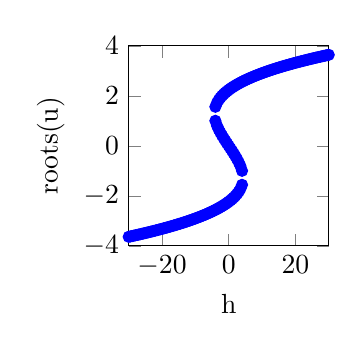
\begin{tikzpicture}

\begin{axis}[%
width=1in,
height=1in,
at={(0.758333in,0.48125in)},
scale only axis,
xmin=-30,
xmax=30,
xlabel={h},
ymin=-4,
ymax=4,
ylabel={roots(u)}
]
\addplot [color=blue,only marks,mark=*,mark options={solid},forget plot]
  table[row sep=crcr]{%
-30	-3.63917834942091\\
};
\addplot [color=blue,only marks,mark=*,mark options={solid},forget plot]
  table[row sep=crcr]{%
-29.5	-3.62471627052737\\
};
\addplot [color=blue,only marks,mark=*,mark options={solid},forget plot]
  table[row sep=crcr]{%
-29	-3.61012080026159\\
};
\addplot [color=blue,only marks,mark=*,mark options={solid},forget plot]
  table[row sep=crcr]{%
-28.5	-3.59538873818504\\
};
\addplot [color=blue,only marks,mark=*,mark options={solid},forget plot]
  table[row sep=crcr]{%
-28	-3.58051675770626\\
};
\addplot [color=blue,only marks,mark=*,mark options={solid},forget plot]
  table[row sep=crcr]{%
-27.5	-3.56550139909124\\
};
\addplot [color=blue,only marks,mark=*,mark options={solid},forget plot]
  table[row sep=crcr]{%
-27	-3.55033906197074\\
};
\addplot [color=blue,only marks,mark=*,mark options={solid},forget plot]
  table[row sep=crcr]{%
-26.5	-3.53502599730006\\
};
\addplot [color=blue,only marks,mark=*,mark options={solid},forget plot]
  table[row sep=crcr]{%
-26	-3.51955829872153\\
};
\addplot [color=blue,only marks,mark=*,mark options={solid},forget plot]
  table[row sep=crcr]{%
-25.5	-3.50393189327477\\
};
\addplot [color=blue,only marks,mark=*,mark options={solid},forget plot]
  table[row sep=crcr]{%
-25	-3.48814253139391\\
};
\addplot [color=blue,only marks,mark=*,mark options={solid},forget plot]
  table[row sep=crcr]{%
-24.5	-3.47218577612358\\
};
\addplot [color=blue,only marks,mark=*,mark options={solid},forget plot]
  table[row sep=crcr]{%
-24	-3.45605699147855\\
};
\addplot [color=blue,only marks,mark=*,mark options={solid},forget plot]
  table[row sep=crcr]{%
-23.5	-3.43975132986214\\
};
\addplot [color=blue,only marks,mark=*,mark options={solid},forget plot]
  table[row sep=crcr]{%
-23	-3.42326371844951\\
};
\addplot [color=blue,only marks,mark=*,mark options={solid},forget plot]
  table[row sep=crcr]{%
-22.5	-3.40658884442979\\
};
\addplot [color=blue,only marks,mark=*,mark options={solid},forget plot]
  table[row sep=crcr]{%
-22	-3.38972113898852\\
};
\addplot [color=blue,only marks,mark=*,mark options={solid},forget plot]
  table[row sep=crcr]{%
-21.5	-3.37265475989695\\
};
\addplot [color=blue,only marks,mark=*,mark options={solid},forget plot]
  table[row sep=crcr]{%
-21	-3.35538357255747\\
};
\addplot [color=blue,only marks,mark=*,mark options={solid},forget plot]
  table[row sep=crcr]{%
-20.5	-3.33790112933523\\
};
\addplot [color=blue,only marks,mark=*,mark options={solid},forget plot]
  table[row sep=crcr]{%
-20	-3.32020064698332\\
};
\addplot [color=blue,only marks,mark=*,mark options={solid},forget plot]
  table[row sep=crcr]{%
-19.5	-3.3022749819426\\
};
\addplot [color=blue,only marks,mark=*,mark options={solid},forget plot]
  table[row sep=crcr]{%
-19	-3.28411660326749\\
};
\addplot [color=blue,only marks,mark=*,mark options={solid},forget plot]
  table[row sep=crcr]{%
-18.5	-3.26571756289342\\
};
\addplot [color=blue,only marks,mark=*,mark options={solid},forget plot]
  table[row sep=crcr]{%
-18	-3.24706946292099\\
};
\addplot [color=blue,only marks,mark=*,mark options={solid},forget plot]
  table[row sep=crcr]{%
-17.5	-3.22816341954377\\
};
\addplot [color=blue,only marks,mark=*,mark options={solid},forget plot]
  table[row sep=crcr]{%
-17	-3.20899002319047\\
};
\addplot [color=blue,only marks,mark=*,mark options={solid},forget plot]
  table[row sep=crcr]{%
-16.5	-3.18953929438578\\
};
\addplot [color=blue,only marks,mark=*,mark options={solid},forget plot]
  table[row sep=crcr]{%
-16	-3.169800634756\\
};
\addplot [color=blue,only marks,mark=*,mark options={solid},forget plot]
  table[row sep=crcr]{%
-15.5	-3.14976277251224\\
};
\addplot [color=blue,only marks,mark=*,mark options={solid},forget plot]
  table[row sep=crcr]{%
-15	-3.12941370163336\\
};
\addplot [color=blue,only marks,mark=*,mark options={solid},forget plot]
  table[row sep=crcr]{%
-14.5	-3.10874061383803\\
};
\addplot [color=blue,only marks,mark=*,mark options={solid},forget plot]
  table[row sep=crcr]{%
-14	-3.08772982227585\\
};
\addplot [color=blue,only marks,mark=*,mark options={solid},forget plot]
  table[row sep=crcr]{%
-13.5	-3.06636667567502\\
};
\addplot [color=blue,only marks,mark=*,mark options={solid},forget plot]
  table[row sep=crcr]{%
-13	-3.04463546145047\\
};
\addplot [color=blue,only marks,mark=*,mark options={solid},forget plot]
  table[row sep=crcr]{%
-12.5	-3.02251929599166\\
};
\addplot [color=blue,only marks,mark=*,mark options={solid},forget plot]
  table[row sep=crcr]{%
-12	-3\\
};
\addplot [color=blue,only marks,mark=*,mark options={solid},forget plot]
  table[row sep=crcr]{%
-11.5	-2.97705795631541\\
};
\addplot [color=blue,only marks,mark=*,mark options={solid},forget plot]
  table[row sep=crcr]{%
-11	-2.95367194713764\\
};
\addplot [color=blue,only marks,mark=*,mark options={solid},forget plot]
  table[row sep=crcr]{%
-10.5	-2.9298189668813\\
};
\addplot [color=blue,only marks,mark=*,mark options={solid},forget plot]
  table[row sep=crcr]{%
-10	-2.90547400606594\\
};
\addplot [color=blue,only marks,mark=*,mark options={solid},forget plot]
  table[row sep=crcr]{%
-9.5	-2.88060980058194\\
};
\addplot [color=blue,only marks,mark=*,mark options={solid},forget plot]
  table[row sep=crcr]{%
-9	-2.85519653932071\\
};
\addplot [color=blue,only marks,mark=*,mark options={solid},forget plot]
  table[row sep=crcr]{%
-8.5	-2.82920152141761\\
};
\addplot [color=blue,only marks,mark=*,mark options={solid},forget plot]
  table[row sep=crcr]{%
-8	-2.80258875210025\\
};
\addplot [color=blue,only marks,mark=*,mark options={solid},forget plot]
  table[row sep=crcr]{%
-7.5	-2.77531846317888\\
};
\addplot [color=blue,only marks,mark=*,mark options={solid},forget plot]
  table[row sep=crcr]{%
-7	-2.74734654030721\\
};
\addplot [color=blue,only marks,mark=*,mark options={solid},forget plot]
  table[row sep=crcr]{%
-6.5	-2.71862383391459\\
};
\addplot [color=blue,only marks,mark=*,mark options={solid},forget plot]
  table[row sep=crcr]{%
-6	-2.68909532363766\\
};
\addplot [color=blue,only marks,mark=*,mark options={solid},forget plot]
  table[row sep=crcr]{%
-5.5	-2.65869909638665\\
};
\addplot [color=blue,only marks,mark=*,mark options={solid},forget plot]
  table[row sep=crcr]{%
-5	-2.62736508471183\\
};
\addplot [color=blue,only marks,mark=*,mark options={solid},forget plot]
  table[row sep=crcr]{%
-4.5	-2.59501349313055\\
};
\addplot [color=blue,only marks,mark=*,mark options={solid},forget plot]
  table[row sep=crcr]{%
-4	-2.56155281280883\\
};
\addplot [color=blue,only marks,mark=*,mark options={solid},forget plot]
  table[row sep=crcr]{%
-4	1.56155281280883\\
};
\addplot [color=blue,only marks,mark=*,mark options={solid},forget plot]
  table[row sep=crcr]{%
-4	1\\
};
\addplot [color=blue,only marks,mark=*,mark options={solid},forget plot]
  table[row sep=crcr]{%
-3.5	-2.52687728514429\\
};
\addplot [color=blue,only marks,mark=*,mark options={solid},forget plot]
  table[row sep=crcr]{%
-3.5	1.72296926110192\\
};
\addplot [color=blue,only marks,mark=*,mark options={solid},forget plot]
  table[row sep=crcr]{%
-3.5	0.803908024042366\\
};
\addplot [color=blue,only marks,mark=*,mark options={solid},forget plot]
  table[row sep=crcr]{%
-3	-2.49086361536103\\
};
\addplot [color=blue,only marks,mark=*,mark options={solid},forget plot]
  table[row sep=crcr]{%
-3	1.83424318431392\\
};
\addplot [color=blue,only marks,mark=*,mark options={solid},forget plot]
  table[row sep=crcr]{%
-3	0.65662043104711\\
};
\addplot [color=blue,only marks,mark=*,mark options={solid},forget plot]
  table[row sep=crcr]{%
-2.5	-2.45336664652482\\
};
\addplot [color=blue,only marks,mark=*,mark options={solid},forget plot]
  table[row sep=crcr]{%
-2.5	1.92363674587377\\
};
\addplot [color=blue,only marks,mark=*,mark options={solid},forget plot]
  table[row sep=crcr]{%
-2.5	0.52972990065105\\
};
\addplot [color=blue,only marks,mark=*,mark options={solid},forget plot]
  table[row sep=crcr]{%
-2	-2.4142135623731\\
};
\addplot [color=blue,only marks,mark=*,mark options={solid},forget plot]
  table[row sep=crcr]{%
-2	2\\
};
\addplot [color=blue,only marks,mark=*,mark options={solid},forget plot]
  table[row sep=crcr]{%
-2	0.414213562373095\\
};
\addplot [color=blue,only marks,mark=*,mark options={solid},forget plot]
  table[row sep=crcr]{%
-1.5	-2.37319595844522\\
};
\addplot [color=blue,only marks,mark=*,mark options={solid},forget plot]
  table[row sep=crcr]{%
-1.5	2.06748146023156\\
};
\addplot [color=blue,only marks,mark=*,mark options={solid},forget plot]
  table[row sep=crcr]{%
-1.5	0.305714498213655\\
};
\addplot [color=blue,only marks,mark=*,mark options={solid},forget plot]
  table[row sep=crcr]{%
-1	-2.33005873956798\\
};
\addplot [color=blue,only marks,mark=*,mark options={solid},forget plot]
  table[row sep=crcr]{%
-1	2.12841906384458\\
};
\addplot [color=blue,only marks,mark=*,mark options={solid},forget plot]
  table[row sep=crcr]{%
-1	0.201639675723405\\
};
\addplot [color=blue,only marks,mark=*,mark options={solid},forget plot]
  table[row sep=crcr]{%
-0.5	-2.28448414134454\\
};
\addplot [color=blue,only marks,mark=*,mark options={solid},forget plot]
  table[row sep=crcr]{%
-0.5	2.18428293165565\\
};
\addplot [color=blue,only marks,mark=*,mark options={solid},forget plot]
  table[row sep=crcr]{%
-0.5	0.100201209688883\\
};
\addplot [color=blue,only marks,mark=*,mark options={solid},forget plot]
  table[row sep=crcr]{%
0	0\\
};
\addplot [color=blue,only marks,mark=*,mark options={solid},forget plot]
  table[row sep=crcr]{%
0	2.23606797749979\\
};
\addplot [color=blue,only marks,mark=*,mark options={solid},forget plot]
  table[row sep=crcr]{%
0	-2.23606797749979\\
};
\addplot [color=blue,only marks,mark=*,mark options={solid},forget plot]
  table[row sep=crcr]{%
0.5	2.28448414134454\\
};
\addplot [color=blue,only marks,mark=*,mark options={solid},forget plot]
  table[row sep=crcr]{%
0.5	-2.18428293165565\\
};
\addplot [color=blue,only marks,mark=*,mark options={solid},forget plot]
  table[row sep=crcr]{%
0.5	-0.100201209688883\\
};
\addplot [color=blue,only marks,mark=*,mark options={solid},forget plot]
  table[row sep=crcr]{%
1	2.33005873956798\\
};
\addplot [color=blue,only marks,mark=*,mark options={solid},forget plot]
  table[row sep=crcr]{%
1	-2.12841906384458\\
};
\addplot [color=blue,only marks,mark=*,mark options={solid},forget plot]
  table[row sep=crcr]{%
1	-0.201639675723405\\
};
\addplot [color=blue,only marks,mark=*,mark options={solid},forget plot]
  table[row sep=crcr]{%
1.5	2.37319595844522\\
};
\addplot [color=blue,only marks,mark=*,mark options={solid},forget plot]
  table[row sep=crcr]{%
1.5	-2.06748146023156\\
};
\addplot [color=blue,only marks,mark=*,mark options={solid},forget plot]
  table[row sep=crcr]{%
1.5	-0.305714498213655\\
};
\addplot [color=blue,only marks,mark=*,mark options={solid},forget plot]
  table[row sep=crcr]{%
2	2.4142135623731\\
};
\addplot [color=blue,only marks,mark=*,mark options={solid},forget plot]
  table[row sep=crcr]{%
2	-2\\
};
\addplot [color=blue,only marks,mark=*,mark options={solid},forget plot]
  table[row sep=crcr]{%
2	-0.414213562373095\\
};
\addplot [color=blue,only marks,mark=*,mark options={solid},forget plot]
  table[row sep=crcr]{%
2.5	2.45336664652482\\
};
\addplot [color=blue,only marks,mark=*,mark options={solid},forget plot]
  table[row sep=crcr]{%
2.5	-1.92363674587377\\
};
\addplot [color=blue,only marks,mark=*,mark options={solid},forget plot]
  table[row sep=crcr]{%
2.5	-0.52972990065105\\
};
\addplot [color=blue,only marks,mark=*,mark options={solid},forget plot]
  table[row sep=crcr]{%
3	2.49086361536103\\
};
\addplot [color=blue,only marks,mark=*,mark options={solid},forget plot]
  table[row sep=crcr]{%
3	-1.83424318431392\\
};
\addplot [color=blue,only marks,mark=*,mark options={solid},forget plot]
  table[row sep=crcr]{%
3	-0.65662043104711\\
};
\addplot [color=blue,only marks,mark=*,mark options={solid},forget plot]
  table[row sep=crcr]{%
3.5	2.52687728514429\\
};
\addplot [color=blue,only marks,mark=*,mark options={solid},forget plot]
  table[row sep=crcr]{%
3.5	-1.72296926110192\\
};
\addplot [color=blue,only marks,mark=*,mark options={solid},forget plot]
  table[row sep=crcr]{%
3.5	-0.803908024042366\\
};
\addplot [color=blue,only marks,mark=*,mark options={solid},forget plot]
  table[row sep=crcr]{%
4	2.56155281280883\\
};
\addplot [color=blue,only marks,mark=*,mark options={solid},forget plot]
  table[row sep=crcr]{%
4	-1.56155281280883\\
};
\addplot [color=blue,only marks,mark=*,mark options={solid},forget plot]
  table[row sep=crcr]{%
4	-1\\
};
\addplot [color=blue,only marks,mark=*,mark options={solid},forget plot]
  table[row sep=crcr]{%
4.5	2.59501349313055\\
};
\addplot [color=blue,only marks,mark=*,mark options={solid},forget plot]
  table[row sep=crcr]{%
5	2.62736508471183\\
};
\addplot [color=blue,only marks,mark=*,mark options={solid},forget plot]
  table[row sep=crcr]{%
5.5	2.65869909638665\\
};
\addplot [color=blue,only marks,mark=*,mark options={solid},forget plot]
  table[row sep=crcr]{%
6	2.68909532363766\\
};
\addplot [color=blue,only marks,mark=*,mark options={solid},forget plot]
  table[row sep=crcr]{%
6.5	2.71862383391459\\
};
\addplot [color=blue,only marks,mark=*,mark options={solid},forget plot]
  table[row sep=crcr]{%
7	2.74734654030721\\
};
\addplot [color=blue,only marks,mark=*,mark options={solid},forget plot]
  table[row sep=crcr]{%
7.5	2.77531846317888\\
};
\addplot [color=blue,only marks,mark=*,mark options={solid},forget plot]
  table[row sep=crcr]{%
8	2.80258875210025\\
};
\addplot [color=blue,only marks,mark=*,mark options={solid},forget plot]
  table[row sep=crcr]{%
8.5	2.82920152141761\\
};
\addplot [color=blue,only marks,mark=*,mark options={solid},forget plot]
  table[row sep=crcr]{%
9	2.85519653932071\\
};
\addplot [color=blue,only marks,mark=*,mark options={solid},forget plot]
  table[row sep=crcr]{%
9.5	2.88060980058194\\
};
\addplot [color=blue,only marks,mark=*,mark options={solid},forget plot]
  table[row sep=crcr]{%
10	2.90547400606594\\
};
\addplot [color=blue,only marks,mark=*,mark options={solid},forget plot]
  table[row sep=crcr]{%
10.5	2.9298189668813\\
};
\addplot [color=blue,only marks,mark=*,mark options={solid},forget plot]
  table[row sep=crcr]{%
11	2.95367194713764\\
};
\addplot [color=blue,only marks,mark=*,mark options={solid},forget plot]
  table[row sep=crcr]{%
11.5	2.97705795631541\\
};
\addplot [color=blue,only marks,mark=*,mark options={solid},forget plot]
  table[row sep=crcr]{%
12	3\\
};
\addplot [color=blue,only marks,mark=*,mark options={solid},forget plot]
  table[row sep=crcr]{%
12.5	3.02251929599166\\
};
\addplot [color=blue,only marks,mark=*,mark options={solid},forget plot]
  table[row sep=crcr]{%
13	3.04463546145047\\
};
\addplot [color=blue,only marks,mark=*,mark options={solid},forget plot]
  table[row sep=crcr]{%
13.5	3.06636667567502\\
};
\addplot [color=blue,only marks,mark=*,mark options={solid},forget plot]
  table[row sep=crcr]{%
14	3.08772982227585\\
};
\addplot [color=blue,only marks,mark=*,mark options={solid},forget plot]
  table[row sep=crcr]{%
14.5	3.10874061383803\\
};
\addplot [color=blue,only marks,mark=*,mark options={solid},forget plot]
  table[row sep=crcr]{%
15	3.12941370163336\\
};
\addplot [color=blue,only marks,mark=*,mark options={solid},forget plot]
  table[row sep=crcr]{%
15.5	3.14976277251224\\
};
\addplot [color=blue,only marks,mark=*,mark options={solid},forget plot]
  table[row sep=crcr]{%
16	3.169800634756\\
};
\addplot [color=blue,only marks,mark=*,mark options={solid},forget plot]
  table[row sep=crcr]{%
16.5	3.18953929438578\\
};
\addplot [color=blue,only marks,mark=*,mark options={solid},forget plot]
  table[row sep=crcr]{%
17	3.20899002319047\\
};
\addplot [color=blue,only marks,mark=*,mark options={solid},forget plot]
  table[row sep=crcr]{%
17.5	3.22816341954377\\
};
\addplot [color=blue,only marks,mark=*,mark options={solid},forget plot]
  table[row sep=crcr]{%
18	3.24706946292099\\
};
\addplot [color=blue,only marks,mark=*,mark options={solid},forget plot]
  table[row sep=crcr]{%
18.5	3.26571756289342\\
};
\addplot [color=blue,only marks,mark=*,mark options={solid},forget plot]
  table[row sep=crcr]{%
19	3.28411660326749\\
};
\addplot [color=blue,only marks,mark=*,mark options={solid},forget plot]
  table[row sep=crcr]{%
19.5	3.3022749819426\\
};
\addplot [color=blue,only marks,mark=*,mark options={solid},forget plot]
  table[row sep=crcr]{%
20	3.32020064698332\\
};
\addplot [color=blue,only marks,mark=*,mark options={solid},forget plot]
  table[row sep=crcr]{%
20.5	3.33790112933523\\
};
\addplot [color=blue,only marks,mark=*,mark options={solid},forget plot]
  table[row sep=crcr]{%
21	3.35538357255747\\
};
\addplot [color=blue,only marks,mark=*,mark options={solid},forget plot]
  table[row sep=crcr]{%
21.5	3.37265475989695\\
};
\addplot [color=blue,only marks,mark=*,mark options={solid},forget plot]
  table[row sep=crcr]{%
22	3.38972113898852\\
};
\addplot [color=blue,only marks,mark=*,mark options={solid},forget plot]
  table[row sep=crcr]{%
22.5	3.40658884442979\\
};
\addplot [color=blue,only marks,mark=*,mark options={solid},forget plot]
  table[row sep=crcr]{%
23	3.42326371844951\\
};
\addplot [color=blue,only marks,mark=*,mark options={solid},forget plot]
  table[row sep=crcr]{%
23.5	3.43975132986214\\
};
\addplot [color=blue,only marks,mark=*,mark options={solid},forget plot]
  table[row sep=crcr]{%
24	3.45605699147855\\
};
\addplot [color=blue,only marks,mark=*,mark options={solid},forget plot]
  table[row sep=crcr]{%
24.5	3.47218577612358\\
};
\addplot [color=blue,only marks,mark=*,mark options={solid},forget plot]
  table[row sep=crcr]{%
25	3.48814253139391\\
};
\addplot [color=blue,only marks,mark=*,mark options={solid},forget plot]
  table[row sep=crcr]{%
25.5	3.50393189327477\\
};
\addplot [color=blue,only marks,mark=*,mark options={solid},forget plot]
  table[row sep=crcr]{%
26	3.51955829872153\\
};
\addplot [color=blue,only marks,mark=*,mark options={solid},forget plot]
  table[row sep=crcr]{%
26.5	3.53502599730006\\
};
\addplot [color=blue,only marks,mark=*,mark options={solid},forget plot]
  table[row sep=crcr]{%
27	3.55033906197074\\
};
\addplot [color=blue,only marks,mark=*,mark options={solid},forget plot]
  table[row sep=crcr]{%
27.5	3.56550139909124\\
};
\addplot [color=blue,only marks,mark=*,mark options={solid},forget plot]
  table[row sep=crcr]{%
28	3.58051675770626\\
};
\addplot [color=blue,only marks,mark=*,mark options={solid},forget plot]
  table[row sep=crcr]{%
28.5	3.59538873818504\\
};
\addplot [color=blue,only marks,mark=*,mark options={solid},forget plot]
  table[row sep=crcr]{%
29	3.61012080026159\\
};
\addplot [color=blue,only marks,mark=*,mark options={solid},forget plot]
  table[row sep=crcr]{%
29.5	3.62471627052737\\
};
\addplot [color=blue,only marks,mark=*,mark options={solid},forget plot]
  table[row sep=crcr]{%
30	3.63917834942091\\
};
\end{axis}
\end{tikzpicture}%
\end{document}
\caption{Solution branches with the function $-\frac{1}{2} u^3 + ru $ numerous colors for different $r\in [-30,30]$ and the constant function $h=5$ in red (left). Root locus plot for the same $r$ values (right).}
\label{fig:one}
% This file was created by matlab2tikz.
% Minimal pgfplots version: 1.3
%
%The latest updates can be retrieved from
%  http://www.mathworks.com/matlabcentral/fileexchange/22022-matlab2tikz
%where you can also make suggestions and rate matlab2tikz.
%
\documentclass[tikz]{standalone}
\usepackage{pgfplots}
\usepackage{grffile}
\pgfplotsset{compat=newest}
\usetikzlibrary{plotmarks}
\usepackage{amsmath}

\begin{document}
\definecolor{mycolor1}{rgb}{0.00000,0.44700,0.74100}%
\definecolor{mycolor2}{rgb}{0.85000,0.32500,0.09800}%
\definecolor{mycolor3}{rgb}{0.92900,0.69400,0.12500}%
\definecolor{mycolor4}{rgb}{0.49400,0.18400,0.55600}%
\definecolor{mycolor5}{rgb}{0.46600,0.67400,0.18800}%
\definecolor{mycolor6}{rgb}{0.30100,0.74500,0.93300}%
\definecolor{mycolor7}{rgb}{0.63500,0.07800,0.18400}%
%
\begin{tikzpicture}

\begin{axis}[%
width=1.520833in,
height=1.565625in,
at={(0.758333in,0.48125in)},
scale only axis,
xmin=-5,
xmax=5,
xlabel={u},
ymin=-100,
ymax=100,
ylabel={f(u)}
]
\addplot [color=mycolor1,solid,forget plot]
  table[row sep=crcr]{%
-5	-25\\
-4.9	-29.351\\
-4.8	-33.408\\
-4.7	-37.177\\
-4.6	-40.664\\
-4.5	-43.875\\
-4.4	-46.816\\
-4.3	-49.493\\
-4.2	-51.912\\
-4.1	-54.079\\
-4	-56\\
-3.9	-57.681\\
-3.8	-59.128\\
-3.7	-60.347\\
-3.6	-61.344\\
-3.5	-62.125\\
-3.4	-62.696\\
-3.3	-63.063\\
-3.2	-63.232\\
-3.1	-63.209\\
-3	-63\\
-2.9	-62.611\\
-2.8	-62.048\\
-2.7	-61.317\\
-2.6	-60.424\\
-2.5	-59.375\\
-2.4	-58.176\\
-2.3	-56.833\\
-2.2	-55.352\\
-2.1	-53.739\\
-2	-52\\
-1.9	-50.141\\
-1.8	-48.168\\
-1.7	-46.087\\
-1.6	-43.904\\
-1.5	-41.625\\
-1.4	-39.256\\
-1.3	-36.803\\
-1.2	-34.272\\
-1.1	-31.669\\
-1	-29\\
-0.899999999999999	-26.271\\
-0.8	-23.488\\
-0.7	-20.657\\
-0.6	-17.784\\
-0.5	-14.875\\
-0.399999999999999	-11.936\\
-0.3	-8.973\\
-0.199999999999999	-5.99199999999998\\
-0.0999999999999996	-2.99899999999999\\
0	0\\
0.0999999999999996	2.99899999999999\\
0.199999999999999	5.99199999999998\\
0.3	8.973\\
0.399999999999999	11.936\\
0.5	14.875\\
0.6	17.784\\
0.7	20.657\\
0.8	23.488\\
0.899999999999999	26.271\\
1	29\\
1.1	31.669\\
1.2	34.272\\
1.3	36.803\\
1.4	39.256\\
1.5	41.625\\
1.6	43.904\\
1.7	46.087\\
1.8	48.168\\
1.9	50.141\\
2	52\\
2.1	53.739\\
2.2	55.352\\
2.3	56.833\\
2.4	58.176\\
2.5	59.375\\
2.6	60.424\\
2.7	61.317\\
2.8	62.048\\
2.9	62.611\\
3	63\\
3.1	63.209\\
3.2	63.232\\
3.3	63.063\\
3.4	62.696\\
3.5	62.125\\
3.6	61.344\\
3.7	60.347\\
3.8	59.128\\
3.9	57.681\\
4	56\\
4.1	54.079\\
4.2	51.912\\
4.3	49.493\\
4.4	46.816\\
4.5	43.875\\
4.6	40.664\\
4.7	37.177\\
4.8	33.408\\
4.9	29.351\\
5	25\\
};
\addplot [color=mycolor2,solid,forget plot]
  table[row sep=crcr]{%
-5	275\\
-4.9	264.649\\
-4.8	254.592\\
-4.7	244.823\\
-4.6	235.336\\
-4.5	226.125\\
-4.4	217.184\\
-4.3	208.507\\
-4.2	200.088\\
-4.1	191.921\\
-4	184\\
-3.9	176.319\\
-3.8	168.872\\
-3.7	161.653\\
-3.6	154.656\\
-3.5	147.875\\
-3.4	141.304\\
-3.3	134.937\\
-3.2	128.768\\
-3.1	122.791\\
-3	117\\
-2.9	111.389\\
-2.8	105.952\\
-2.7	100.683\\
-2.6	95.576\\
-2.5	90.625\\
-2.4	85.824\\
-2.3	81.167\\
-2.2	76.648\\
-2.1	72.261\\
-2	68\\
-1.9	63.859\\
-1.8	59.832\\
-1.7	55.913\\
-1.6	52.096\\
-1.5	48.375\\
-1.4	44.744\\
-1.3	41.197\\
-1.2	37.728\\
-1.1	34.331\\
-1	31\\
-0.899999999999999	27.729\\
-0.8	24.512\\
-0.7	21.343\\
-0.6	18.216\\
-0.5	15.125\\
-0.399999999999999	12.064\\
-0.3	9.02699999999999\\
-0.199999999999999	6.00799999999998\\
-0.0999999999999996	3.00099999999999\\
0	-0\\
0.0999999999999996	-3.00099999999999\\
0.199999999999999	-6.00799999999998\\
0.3	-9.02699999999999\\
0.399999999999999	-12.064\\
0.5	-15.125\\
0.6	-18.216\\
0.7	-21.343\\
0.8	-24.512\\
0.899999999999999	-27.729\\
1	-31\\
1.1	-34.331\\
1.2	-37.728\\
1.3	-41.197\\
1.4	-44.744\\
1.5	-48.375\\
1.6	-52.096\\
1.7	-55.913\\
1.8	-59.832\\
1.9	-63.859\\
2	-68\\
2.1	-72.261\\
2.2	-76.648\\
2.3	-81.167\\
2.4	-85.824\\
2.5	-90.625\\
2.6	-95.576\\
2.7	-100.683\\
2.8	-105.952\\
2.9	-111.389\\
3	-117\\
3.1	-122.791\\
3.2	-128.768\\
3.3	-134.937\\
3.4	-141.304\\
3.5	-147.875\\
3.6	-154.656\\
3.7	-161.653\\
3.8	-168.872\\
3.9	-176.319\\
4	-184\\
4.1	-191.921\\
4.2	-200.088\\
4.3	-208.507\\
4.4	-217.184\\
4.5	-226.125\\
4.6	-235.336\\
4.7	-244.823\\
4.8	-254.592\\
4.9	-264.649\\
5	-275\\
};
\addplot [color=mycolor3,solid,forget plot]
  table[row sep=crcr]{%
-5	241.666666666667\\
-4.9	231.982333333333\\
-4.8	222.592\\
-4.7	213.489666666667\\
-4.6	204.669333333333\\
-4.5	196.125\\
-4.4	187.850666666667\\
-4.3	179.840333333333\\
-4.2	172.088\\
-4.1	164.587666666667\\
-4	157.333333333333\\
-3.9	150.319\\
-3.8	143.538666666667\\
-3.7	136.986333333333\\
-3.6	130.656\\
-3.5	124.541666666667\\
-3.4	118.637333333333\\
-3.3	112.937\\
-3.2	107.434666666667\\
-3.1	102.124333333333\\
-3	97\\
-2.9	92.0556666666667\\
-2.8	87.2853333333333\\
-2.7	82.683\\
-2.6	78.2426666666667\\
-2.5	73.9583333333333\\
-2.4	69.824\\
-2.3	65.8336666666667\\
-2.2	61.9813333333333\\
-2.1	58.261\\
-2	54.6666666666667\\
-1.9	51.1923333333333\\
-1.8	47.832\\
-1.7	44.5796666666667\\
-1.6	41.4293333333333\\
-1.5	38.375\\
-1.4	35.4106666666667\\
-1.3	32.5303333333333\\
-1.2	29.728\\
-1.1	26.9976666666667\\
-1	24.3333333333333\\
-0.899999999999999	21.729\\
-0.8	19.1786666666667\\
-0.7	16.6763333333333\\
-0.6	14.216\\
-0.5	11.7916666666667\\
-0.399999999999999	9.39733333333332\\
-0.3	7.027\\
-0.199999999999999	4.67466666666665\\
-0.0999999999999996	2.33433333333332\\
0	-0\\
0.0999999999999996	-2.33433333333332\\
0.199999999999999	-4.67466666666665\\
0.3	-7.027\\
0.399999999999999	-9.39733333333332\\
0.5	-11.7916666666667\\
0.6	-14.216\\
0.7	-16.6763333333333\\
0.8	-19.1786666666667\\
0.899999999999999	-21.729\\
1	-24.3333333333333\\
1.1	-26.9976666666667\\
1.2	-29.728\\
1.3	-32.5303333333333\\
1.4	-35.4106666666667\\
1.5	-38.375\\
1.6	-41.4293333333333\\
1.7	-44.5796666666667\\
1.8	-47.832\\
1.9	-51.1923333333333\\
2	-54.6666666666667\\
2.1	-58.261\\
2.2	-61.9813333333333\\
2.3	-65.8336666666667\\
2.4	-69.824\\
2.5	-73.9583333333333\\
2.6	-78.2426666666667\\
2.7	-82.683\\
2.8	-87.2853333333333\\
2.9	-92.0556666666667\\
3	-97\\
3.1	-102.124333333333\\
3.2	-107.434666666667\\
3.3	-112.937\\
3.4	-118.637333333333\\
3.5	-124.541666666667\\
3.6	-130.656\\
3.7	-136.986333333333\\
3.8	-143.538666666667\\
3.9	-150.319\\
4	-157.333333333333\\
4.1	-164.587666666667\\
4.2	-172.088\\
4.3	-179.840333333333\\
4.4	-187.850666666667\\
4.5	-196.125\\
4.6	-204.669333333333\\
4.7	-213.489666666667\\
4.8	-222.592\\
4.9	-231.982333333333\\
5	-241.666666666667\\
};
\addplot [color=mycolor4,solid,forget plot]
  table[row sep=crcr]{%
-5	208.333333333333\\
-4.9	199.315666666667\\
-4.8	190.592\\
-4.7	182.156333333333\\
-4.6	174.002666666667\\
-4.5	166.125\\
-4.4	158.517333333333\\
-4.3	151.173666666667\\
-4.2	144.088\\
-4.1	137.254333333333\\
-4	130.666666666667\\
-3.9	124.319\\
-3.8	118.205333333333\\
-3.7	112.319666666667\\
-3.6	106.656\\
-3.5	101.208333333333\\
-3.4	95.9706666666667\\
-3.3	90.937\\
-3.2	86.1013333333333\\
-3.1	81.4576666666666\\
-3	77\\
-2.9	72.7223333333333\\
-2.8	68.6186666666667\\
-2.7	64.683\\
-2.6	60.9093333333333\\
-2.5	57.2916666666667\\
-2.4	53.824\\
-2.3	50.5003333333333\\
-2.2	47.3146666666667\\
-2.1	44.261\\
-2	41.3333333333333\\
-1.9	38.5256666666667\\
-1.8	35.832\\
-1.7	33.2463333333333\\
-1.6	30.7626666666667\\
-1.5	28.375\\
-1.4	26.0773333333333\\
-1.3	23.8636666666667\\
-1.2	21.728\\
-1.1	19.6643333333333\\
-1	17.6666666666667\\
-0.899999999999999	15.729\\
-0.8	13.8453333333333\\
-0.7	12.0096666666667\\
-0.6	10.216\\
-0.5	8.45833333333333\\
-0.399999999999999	6.73066666666666\\
-0.3	5.027\\
-0.199999999999999	3.34133333333332\\
-0.0999999999999996	1.66766666666666\\
0	-0\\
0.0999999999999996	-1.66766666666666\\
0.199999999999999	-3.34133333333332\\
0.3	-5.027\\
0.399999999999999	-6.73066666666666\\
0.5	-8.45833333333333\\
0.6	-10.216\\
0.7	-12.0096666666667\\
0.8	-13.8453333333333\\
0.899999999999999	-15.729\\
1	-17.6666666666667\\
1.1	-19.6643333333333\\
1.2	-21.728\\
1.3	-23.8636666666667\\
1.4	-26.0773333333333\\
1.5	-28.375\\
1.6	-30.7626666666667\\
1.7	-33.2463333333333\\
1.8	-35.832\\
1.9	-38.5256666666667\\
2	-41.3333333333333\\
2.1	-44.261\\
2.2	-47.3146666666667\\
2.3	-50.5003333333333\\
2.4	-53.824\\
2.5	-57.2916666666667\\
2.6	-60.9093333333333\\
2.7	-64.683\\
2.8	-68.6186666666667\\
2.9	-72.7223333333333\\
3	-77\\
3.1	-81.4576666666666\\
3.2	-86.1013333333333\\
3.3	-90.937\\
3.4	-95.9706666666667\\
3.5	-101.208333333333\\
3.6	-106.656\\
3.7	-112.319666666667\\
3.8	-118.205333333333\\
3.9	-124.319\\
4	-130.666666666667\\
4.1	-137.254333333333\\
4.2	-144.088\\
4.3	-151.173666666667\\
4.4	-158.517333333333\\
4.5	-166.125\\
4.6	-174.002666666667\\
4.7	-182.156333333333\\
4.8	-190.592\\
4.9	-199.315666666667\\
5	-208.333333333333\\
};
\addplot [color=mycolor5,solid,forget plot]
  table[row sep=crcr]{%
-5	175\\
-4.9	166.649\\
-4.8	158.592\\
-4.7	150.823\\
-4.6	143.336\\
-4.5	136.125\\
-4.4	129.184\\
-4.3	122.507\\
-4.2	116.088\\
-4.1	109.921\\
-4	104\\
-3.9	98.319\\
-3.8	92.872\\
-3.7	87.653\\
-3.6	82.656\\
-3.5	77.875\\
-3.4	73.304\\
-3.3	68.937\\
-3.2	64.768\\
-3.1	60.791\\
-3	57\\
-2.9	53.389\\
-2.8	49.952\\
-2.7	46.683\\
-2.6	43.576\\
-2.5	40.625\\
-2.4	37.824\\
-2.3	35.167\\
-2.2	32.648\\
-2.1	30.261\\
-2	28\\
-1.9	25.859\\
-1.8	23.832\\
-1.7	21.913\\
-1.6	20.096\\
-1.5	18.375\\
-1.4	16.744\\
-1.3	15.197\\
-1.2	13.728\\
-1.1	12.331\\
-1	11\\
-0.899999999999999	9.72899999999999\\
-0.8	8.512\\
-0.7	7.343\\
-0.6	6.216\\
-0.5	5.125\\
-0.399999999999999	4.06399999999999\\
-0.3	3.027\\
-0.199999999999999	2.00799999999999\\
-0.0999999999999996	1.001\\
0	-0\\
0.0999999999999996	-1.001\\
0.199999999999999	-2.00799999999999\\
0.3	-3.027\\
0.399999999999999	-4.06399999999999\\
0.5	-5.125\\
0.6	-6.216\\
0.7	-7.343\\
0.8	-8.512\\
0.899999999999999	-9.72899999999999\\
1	-11\\
1.1	-12.331\\
1.2	-13.728\\
1.3	-15.197\\
1.4	-16.744\\
1.5	-18.375\\
1.6	-20.096\\
1.7	-21.913\\
1.8	-23.832\\
1.9	-25.859\\
2	-28\\
2.1	-30.261\\
2.2	-32.648\\
2.3	-35.167\\
2.4	-37.824\\
2.5	-40.625\\
2.6	-43.576\\
2.7	-46.683\\
2.8	-49.952\\
2.9	-53.389\\
3	-57\\
3.1	-60.791\\
3.2	-64.768\\
3.3	-68.937\\
3.4	-73.304\\
3.5	-77.875\\
3.6	-82.656\\
3.7	-87.653\\
3.8	-92.872\\
3.9	-98.319\\
4	-104\\
4.1	-109.921\\
4.2	-116.088\\
4.3	-122.507\\
4.4	-129.184\\
4.5	-136.125\\
4.6	-143.336\\
4.7	-150.823\\
4.8	-158.592\\
4.9	-166.649\\
5	-175\\
};
\addplot [color=mycolor6,solid,forget plot]
  table[row sep=crcr]{%
-5	141.666666666667\\
-4.9	133.982333333333\\
-4.8	126.592\\
-4.7	119.489666666667\\
-4.6	112.669333333333\\
-4.5	106.125\\
-4.4	99.8506666666667\\
-4.3	93.8403333333333\\
-4.2	88.088\\
-4.1	82.5876666666666\\
-4	77.3333333333333\\
-3.9	72.319\\
-3.8	67.5386666666667\\
-3.7	62.9863333333333\\
-3.6	58.656\\
-3.5	54.5416666666667\\
-3.4	50.6373333333333\\
-3.3	46.937\\
-3.2	43.4346666666667\\
-3.1	40.1243333333333\\
-3	37\\
-2.9	34.0556666666667\\
-2.8	31.2853333333333\\
-2.7	28.683\\
-2.6	26.2426666666667\\
-2.5	23.9583333333333\\
-2.4	21.824\\
-2.3	19.8336666666667\\
-2.2	17.9813333333333\\
-2.1	16.261\\
-2	14.6666666666667\\
-1.9	13.1923333333333\\
-1.8	11.832\\
-1.7	10.5796666666667\\
-1.6	9.42933333333333\\
-1.5	8.375\\
-1.4	7.41066666666666\\
-1.3	6.53033333333333\\
-1.2	5.728\\
-1.1	4.99766666666666\\
-1	4.33333333333333\\
-0.899999999999999	3.729\\
-0.8	3.17866666666666\\
-0.7	2.67633333333333\\
-0.6	2.216\\
-0.5	1.79166666666667\\
-0.399999999999999	1.39733333333333\\
-0.3	1.027\\
-0.199999999999999	0.674666666666664\\
-0.0999999999999996	0.334333333333332\\
0	-0\\
0.0999999999999996	-0.334333333333332\\
0.199999999999999	-0.674666666666664\\
0.3	-1.027\\
0.399999999999999	-1.39733333333333\\
0.5	-1.79166666666667\\
0.6	-2.216\\
0.7	-2.67633333333333\\
0.8	-3.17866666666666\\
0.899999999999999	-3.729\\
1	-4.33333333333333\\
1.1	-4.99766666666666\\
1.2	-5.728\\
1.3	-6.53033333333333\\
1.4	-7.41066666666666\\
1.5	-8.375\\
1.6	-9.42933333333333\\
1.7	-10.5796666666667\\
1.8	-11.832\\
1.9	-13.1923333333333\\
2	-14.6666666666667\\
2.1	-16.261\\
2.2	-17.9813333333333\\
2.3	-19.8336666666667\\
2.4	-21.824\\
2.5	-23.9583333333333\\
2.6	-26.2426666666667\\
2.7	-28.683\\
2.8	-31.2853333333333\\
2.9	-34.0556666666667\\
3	-37\\
3.1	-40.1243333333333\\
3.2	-43.4346666666667\\
3.3	-46.937\\
3.4	-50.6373333333333\\
3.5	-54.5416666666667\\
3.6	-58.656\\
3.7	-62.9863333333333\\
3.8	-67.5386666666667\\
3.9	-72.319\\
4	-77.3333333333333\\
4.1	-82.5876666666666\\
4.2	-88.088\\
4.3	-93.8403333333333\\
4.4	-99.8506666666667\\
4.5	-106.125\\
4.6	-112.669333333333\\
4.7	-119.489666666667\\
4.8	-126.592\\
4.9	-133.982333333333\\
5	-141.666666666667\\
};
\addplot [color=mycolor7,solid,forget plot]
  table[row sep=crcr]{%
-5	108.333333333333\\
-4.9	101.315666666667\\
-4.8	94.592\\
-4.7	88.1563333333333\\
-4.6	82.0026666666666\\
-4.5	76.125\\
-4.4	70.5173333333333\\
-4.3	65.1736666666666\\
-4.2	60.088\\
-4.1	55.2543333333333\\
-4	50.6666666666667\\
-3.9	46.319\\
-3.8	42.2053333333333\\
-3.7	38.3196666666667\\
-3.6	34.656\\
-3.5	31.2083333333333\\
-3.4	27.9706666666667\\
-3.3	24.937\\
-3.2	22.1013333333333\\
-3.1	19.4576666666667\\
-3	17\\
-2.9	14.7223333333333\\
-2.8	12.6186666666667\\
-2.7	10.683\\
-2.6	8.90933333333332\\
-2.5	7.29166666666666\\
-2.4	5.82399999999999\\
-2.3	4.50033333333333\\
-2.2	3.31466666666666\\
-2.1	2.26099999999999\\
-2	1.33333333333333\\
-1.9	0.525666666666662\\
-1.8	-0.168000000000005\\
-1.7	-0.753666666666672\\
-1.6	-1.23733333333334\\
-1.5	-1.625\\
-1.4	-1.92266666666667\\
-1.3	-2.13633333333334\\
-1.2	-2.272\\
-1.1	-2.33566666666667\\
-1	-2.33333333333334\\
-0.899999999999999	-2.271\\
-0.8	-2.15466666666667\\
-0.7	-1.99033333333334\\
-0.6	-1.784\\
-0.5	-1.54166666666667\\
-0.399999999999999	-1.26933333333333\\
-0.3	-0.973\\
-0.199999999999999	-0.658666666666665\\
-0.0999999999999996	-0.332333333333332\\
0	0\\
0.0999999999999996	0.332333333333332\\
0.199999999999999	0.658666666666665\\
0.3	0.973\\
0.399999999999999	1.26933333333333\\
0.5	1.54166666666667\\
0.6	1.784\\
0.7	1.99033333333334\\
0.8	2.15466666666667\\
0.899999999999999	2.271\\
1	2.33333333333334\\
1.1	2.33566666666667\\
1.2	2.272\\
1.3	2.13633333333334\\
1.4	1.92266666666667\\
1.5	1.625\\
1.6	1.23733333333334\\
1.7	0.753666666666672\\
1.8	0.168000000000005\\
1.9	-0.525666666666662\\
2	-1.33333333333333\\
2.1	-2.26099999999999\\
2.2	-3.31466666666666\\
2.3	-4.50033333333333\\
2.4	-5.82399999999999\\
2.5	-7.29166666666666\\
2.6	-8.90933333333332\\
2.7	-10.683\\
2.8	-12.6186666666667\\
2.9	-14.7223333333333\\
3	-17\\
3.1	-19.4576666666667\\
3.2	-22.1013333333333\\
3.3	-24.937\\
3.4	-27.9706666666667\\
3.5	-31.2083333333333\\
3.6	-34.656\\
3.7	-38.3196666666667\\
3.8	-42.2053333333333\\
3.9	-46.319\\
4	-50.6666666666667\\
4.1	-55.2543333333333\\
4.2	-60.088\\
4.3	-65.1736666666666\\
4.4	-70.5173333333333\\
4.5	-76.125\\
4.6	-82.0026666666666\\
4.7	-88.1563333333333\\
4.8	-94.592\\
4.9	-101.315666666667\\
5	-108.333333333333\\
};
\addplot [color=mycolor1,solid,forget plot]
  table[row sep=crcr]{%
-5	75\\
-4.9	68.649\\
-4.8	62.592\\
-4.7	56.823\\
-4.6	51.336\\
-4.5	46.125\\
-4.4	41.184\\
-4.3	36.507\\
-4.2	32.088\\
-4.1	27.921\\
-4	24\\
-3.9	20.319\\
-3.8	16.872\\
-3.7	13.653\\
-3.6	10.656\\
-3.5	7.875\\
-3.4	5.30399999999999\\
-3.3	2.937\\
-3.2	0.768000000000008\\
-3.1	-1.20900000000001\\
-3	-3\\
-2.9	-4.611\\
-2.8	-6.04800000000001\\
-2.7	-7.317\\
-2.6	-8.424\\
-2.5	-9.375\\
-2.4	-10.176\\
-2.3	-10.833\\
-2.2	-11.352\\
-2.1	-11.739\\
-2	-12\\
-1.9	-12.141\\
-1.8	-12.168\\
-1.7	-12.087\\
-1.6	-11.904\\
-1.5	-11.625\\
-1.4	-11.256\\
-1.3	-10.803\\
-1.2	-10.272\\
-1.1	-9.669\\
-1	-9\\
-0.899999999999999	-8.271\\
-0.8	-7.488\\
-0.7	-6.657\\
-0.6	-5.784\\
-0.5	-4.875\\
-0.399999999999999	-3.936\\
-0.3	-2.973\\
-0.199999999999999	-1.99199999999999\\
-0.0999999999999996	-0.998999999999996\\
0	0\\
0.0999999999999996	0.998999999999996\\
0.199999999999999	1.99199999999999\\
0.3	2.973\\
0.399999999999999	3.936\\
0.5	4.875\\
0.6	5.784\\
0.7	6.657\\
0.8	7.488\\
0.899999999999999	8.271\\
1	9\\
1.1	9.669\\
1.2	10.272\\
1.3	10.803\\
1.4	11.256\\
1.5	11.625\\
1.6	11.904\\
1.7	12.087\\
1.8	12.168\\
1.9	12.141\\
2	12\\
2.1	11.739\\
2.2	11.352\\
2.3	10.833\\
2.4	10.176\\
2.5	9.375\\
2.6	8.424\\
2.7	7.317\\
2.8	6.04800000000001\\
2.9	4.611\\
3	3\\
3.1	1.20900000000001\\
3.2	-0.768000000000008\\
3.3	-2.937\\
3.4	-5.30399999999999\\
3.5	-7.875\\
3.6	-10.656\\
3.7	-13.653\\
3.8	-16.872\\
3.9	-20.319\\
4	-24\\
4.1	-27.921\\
4.2	-32.088\\
4.3	-36.507\\
4.4	-41.184\\
4.5	-46.125\\
4.6	-51.336\\
4.7	-56.823\\
4.8	-62.592\\
4.9	-68.649\\
5	-75\\
};
\addplot [color=mycolor2,solid,forget plot]
  table[row sep=crcr]{%
-5	41.6666666666667\\
-4.9	35.9823333333334\\
-4.8	30.592\\
-4.7	25.4896666666667\\
-4.6	20.6693333333333\\
-4.5	16.125\\
-4.4	11.8506666666667\\
-4.3	7.84033333333333\\
-4.2	4.08800000000001\\
-4.1	0.587666666666664\\
-4	-2.66666666666666\\
-3.9	-5.68099999999999\\
-3.8	-8.46133333333333\\
-3.7	-11.0136666666667\\
-3.6	-13.344\\
-3.5	-15.4583333333333\\
-3.4	-17.3626666666667\\
-3.3	-19.063\\
-3.2	-20.5653333333333\\
-3.1	-21.8756666666667\\
-3	-23\\
-2.9	-23.9443333333333\\
-2.8	-24.7146666666667\\
-2.7	-25.317\\
-2.6	-25.7573333333333\\
-2.5	-26.0416666666667\\
-2.4	-26.176\\
-2.3	-26.1663333333333\\
-2.2	-26.0186666666667\\
-2.1	-25.739\\
-2	-25.3333333333333\\
-1.9	-24.8076666666667\\
-1.8	-24.168\\
-1.7	-23.4203333333333\\
-1.6	-22.5706666666667\\
-1.5	-21.625\\
-1.4	-20.5893333333333\\
-1.3	-19.4696666666667\\
-1.2	-18.272\\
-1.1	-17.0023333333333\\
-1	-15.6666666666667\\
-0.899999999999999	-14.271\\
-0.8	-12.8213333333333\\
-0.7	-11.3236666666667\\
-0.6	-9.78399999999999\\
-0.5	-8.20833333333333\\
-0.399999999999999	-6.60266666666666\\
-0.3	-4.973\\
-0.199999999999999	-3.32533333333332\\
-0.0999999999999996	-1.66566666666666\\
0	0\\
0.0999999999999996	1.66566666666666\\
0.199999999999999	3.32533333333332\\
0.3	4.973\\
0.399999999999999	6.60266666666666\\
0.5	8.20833333333333\\
0.6	9.78399999999999\\
0.7	11.3236666666667\\
0.8	12.8213333333333\\
0.899999999999999	14.271\\
1	15.6666666666667\\
1.1	17.0023333333333\\
1.2	18.272\\
1.3	19.4696666666667\\
1.4	20.5893333333333\\
1.5	21.625\\
1.6	22.5706666666667\\
1.7	23.4203333333333\\
1.8	24.168\\
1.9	24.8076666666667\\
2	25.3333333333333\\
2.1	25.739\\
2.2	26.0186666666667\\
2.3	26.1663333333333\\
2.4	26.176\\
2.5	26.0416666666667\\
2.6	25.7573333333333\\
2.7	25.317\\
2.8	24.7146666666667\\
2.9	23.9443333333333\\
3	23\\
3.1	21.8756666666667\\
3.2	20.5653333333333\\
3.3	19.063\\
3.4	17.3626666666667\\
3.5	15.4583333333333\\
3.6	13.344\\
3.7	11.0136666666667\\
3.8	8.46133333333333\\
3.9	5.68099999999999\\
4	2.66666666666666\\
4.1	-0.587666666666664\\
4.2	-4.08800000000001\\
4.3	-7.84033333333333\\
4.4	-11.8506666666667\\
4.5	-16.125\\
4.6	-20.6693333333333\\
4.7	-25.4896666666667\\
4.8	-30.592\\
4.9	-35.9823333333334\\
5	-41.6666666666667\\
};
\addplot [color=mycolor3,solid,forget plot]
  table[row sep=crcr]{%
-5	8.33333333333331\\
-4.9	3.31566666666667\\
-4.8	-1.40800000000003\\
-4.7	-5.84366666666668\\
-4.6	-9.99733333333336\\
-4.5	-13.875\\
-4.4	-17.4826666666667\\
-4.3	-20.8263333333334\\
-4.2	-23.912\\
-4.1	-26.7456666666667\\
-4	-29.3333333333333\\
-3.9	-31.681\\
-3.8	-33.7946666666667\\
-3.7	-35.6803333333333\\
-3.6	-37.344\\
-3.5	-38.7916666666667\\
-3.4	-40.0293333333333\\
-3.3	-41.063\\
-3.2	-41.8986666666667\\
-3.1	-42.5423333333333\\
-3	-43\\
-2.9	-43.2776666666667\\
-2.8	-43.3813333333333\\
-2.7	-43.317\\
-2.6	-43.0906666666667\\
-2.5	-42.7083333333333\\
-2.4	-42.176\\
-2.3	-41.4996666666667\\
-2.2	-40.6853333333333\\
-2.1	-39.739\\
-2	-38.6666666666667\\
-1.9	-37.4743333333333\\
-1.8	-36.168\\
-1.7	-34.7536666666667\\
-1.6	-33.2373333333333\\
-1.5	-31.625\\
-1.4	-29.9226666666667\\
-1.3	-28.1363333333333\\
-1.2	-26.272\\
-1.1	-24.3356666666667\\
-1	-22.3333333333333\\
-0.899999999999999	-20.271\\
-0.8	-18.1546666666667\\
-0.7	-15.9903333333333\\
-0.6	-13.784\\
-0.5	-11.5416666666667\\
-0.399999999999999	-9.26933333333332\\
-0.3	-6.973\\
-0.199999999999999	-4.65866666666665\\
-0.0999999999999996	-2.33233333333333\\
0	0\\
0.0999999999999996	2.33233333333333\\
0.199999999999999	4.65866666666665\\
0.3	6.973\\
0.399999999999999	9.26933333333332\\
0.5	11.5416666666667\\
0.6	13.784\\
0.7	15.9903333333333\\
0.8	18.1546666666667\\
0.899999999999999	20.271\\
1	22.3333333333333\\
1.1	24.3356666666667\\
1.2	26.272\\
1.3	28.1363333333333\\
1.4	29.9226666666667\\
1.5	31.625\\
1.6	33.2373333333333\\
1.7	34.7536666666667\\
1.8	36.168\\
1.9	37.4743333333333\\
2	38.6666666666667\\
2.1	39.739\\
2.2	40.6853333333333\\
2.3	41.4996666666667\\
2.4	42.176\\
2.5	42.7083333333333\\
2.6	43.0906666666667\\
2.7	43.317\\
2.8	43.3813333333333\\
2.9	43.2776666666667\\
3	43\\
3.1	42.5423333333333\\
3.2	41.8986666666667\\
3.3	41.063\\
3.4	40.0293333333333\\
3.5	38.7916666666667\\
3.6	37.344\\
3.7	35.6803333333333\\
3.8	33.7946666666667\\
3.9	31.681\\
4	29.3333333333333\\
4.1	26.7456666666667\\
4.2	23.912\\
4.3	20.8263333333334\\
4.4	17.4826666666667\\
4.5	13.875\\
4.6	9.99733333333336\\
4.7	5.84366666666668\\
4.8	1.40800000000003\\
4.9	-3.31566666666667\\
5	-8.33333333333331\\
};
\addplot [color=red,only marks,mark=*,mark size={0.5},forget plot]
  table[row sep=crcr]{%
-5	0\\
};
\addplot [color=red,only marks,mark=*,mark size={0.5},forget plot]
  table[row sep=crcr]{%
-4.9	0\\
};
\addplot [color=red,only marks,mark=*,mark size={0.5},forget plot]
  table[row sep=crcr]{%
-4.8	0\\
};
\addplot [color=red,only marks,mark=*,mark size={0.5},forget plot]
  table[row sep=crcr]{%
-4.7	0\\
};
\addplot [color=red,only marks,mark=*,mark size={0.5},forget plot]
  table[row sep=crcr]{%
-4.6	0\\
};
\addplot [color=red,only marks,mark=*,mark size={0.5},forget plot]
  table[row sep=crcr]{%
-4.5	0\\
};
\addplot [color=red,only marks,mark=*,mark size={0.5},forget plot]
  table[row sep=crcr]{%
-4.4	0\\
};
\addplot [color=red,only marks,mark=*,mark size={0.5},forget plot]
  table[row sep=crcr]{%
-4.3	0\\
};
\addplot [color=red,only marks,mark=*,mark size={0.5},forget plot]
  table[row sep=crcr]{%
-4.2	0\\
};
\addplot [color=red,only marks,mark=*,mark size={0.5},forget plot]
  table[row sep=crcr]{%
-4.1	0\\
};
\addplot [color=red,only marks,mark=*,mark size={0.5},forget plot]
  table[row sep=crcr]{%
-4	0\\
};
\addplot [color=red,only marks,mark=*,mark size={0.5},forget plot]
  table[row sep=crcr]{%
-3.9	0\\
};
\addplot [color=red,only marks,mark=*,mark size={0.5},forget plot]
  table[row sep=crcr]{%
-3.8	0\\
};
\addplot [color=red,only marks,mark=*,mark size={0.5},forget plot]
  table[row sep=crcr]{%
-3.7	0\\
};
\addplot [color=red,only marks,mark=*,mark size={0.5},forget plot]
  table[row sep=crcr]{%
-3.6	0\\
};
\addplot [color=red,only marks,mark=*,mark size={0.5},forget plot]
  table[row sep=crcr]{%
-3.5	0\\
};
\addplot [color=red,only marks,mark=*,mark size={0.5},forget plot]
  table[row sep=crcr]{%
-3.4	0\\
};
\addplot [color=red,only marks,mark=*,mark size={0.5},forget plot]
  table[row sep=crcr]{%
-3.3	0\\
};
\addplot [color=red,only marks,mark=*,mark size={0.5},forget plot]
  table[row sep=crcr]{%
-3.2	0\\
};
\addplot [color=red,only marks,mark=*,mark size={0.5},forget plot]
  table[row sep=crcr]{%
-3.1	0\\
};
\addplot [color=red,only marks,mark=*,mark size={0.5},forget plot]
  table[row sep=crcr]{%
-3	0\\
};
\addplot [color=red,only marks,mark=*,mark size={0.5},forget plot]
  table[row sep=crcr]{%
-2.9	0\\
};
\addplot [color=red,only marks,mark=*,mark size={0.5},forget plot]
  table[row sep=crcr]{%
-2.8	0\\
};
\addplot [color=red,only marks,mark=*,mark size={0.5},forget plot]
  table[row sep=crcr]{%
-2.7	0\\
};
\addplot [color=red,only marks,mark=*,mark size={0.5},forget plot]
  table[row sep=crcr]{%
-2.6	0\\
};
\addplot [color=red,only marks,mark=*,mark size={0.5},forget plot]
  table[row sep=crcr]{%
-2.5	0\\
};
\addplot [color=red,only marks,mark=*,mark size={0.5},forget plot]
  table[row sep=crcr]{%
-2.4	0\\
};
\addplot [color=red,only marks,mark=*,mark size={0.5},forget plot]
  table[row sep=crcr]{%
-2.3	0\\
};
\addplot [color=red,only marks,mark=*,mark size={0.5},forget plot]
  table[row sep=crcr]{%
-2.2	0\\
};
\addplot [color=red,only marks,mark=*,mark size={0.5},forget plot]
  table[row sep=crcr]{%
-2.1	0\\
};
\addplot [color=red,only marks,mark=*,mark size={0.5},forget plot]
  table[row sep=crcr]{%
-2	0\\
};
\addplot [color=red,only marks,mark=*,mark size={0.5},forget plot]
  table[row sep=crcr]{%
-1.9	0\\
};
\addplot [color=red,only marks,mark=*,mark size={0.5},forget plot]
  table[row sep=crcr]{%
-1.8	0\\
};
\addplot [color=red,only marks,mark=*,mark size={0.5},forget plot]
  table[row sep=crcr]{%
-1.7	0\\
};
\addplot [color=red,only marks,mark=*,mark size={0.5},forget plot]
  table[row sep=crcr]{%
-1.6	0\\
};
\addplot [color=red,only marks,mark=*,mark size={0.5},forget plot]
  table[row sep=crcr]{%
-1.5	0\\
};
\addplot [color=red,only marks,mark=*,mark size={0.5},forget plot]
  table[row sep=crcr]{%
-1.4	0\\
};
\addplot [color=red,only marks,mark=*,mark size={0.5},forget plot]
  table[row sep=crcr]{%
-1.3	0\\
};
\addplot [color=red,only marks,mark=*,mark size={0.5},forget plot]
  table[row sep=crcr]{%
-1.2	0\\
};
\addplot [color=red,only marks,mark=*,mark size={0.5},forget plot]
  table[row sep=crcr]{%
-1.1	0\\
};
\addplot [color=red,only marks,mark=*,mark size={0.5},forget plot]
  table[row sep=crcr]{%
-1	0\\
};
\addplot [color=red,only marks,mark=*,mark size={0.5},forget plot]
  table[row sep=crcr]{%
-0.899999999999999	0\\
};
\addplot [color=red,only marks,mark=*,mark size={0.5},forget plot]
  table[row sep=crcr]{%
-0.8	0\\
};
\addplot [color=red,only marks,mark=*,mark size={0.5},forget plot]
  table[row sep=crcr]{%
-0.7	0\\
};
\addplot [color=red,only marks,mark=*,mark size={0.5},forget plot]
  table[row sep=crcr]{%
-0.6	0\\
};
\addplot [color=red,only marks,mark=*,mark size={0.5},forget plot]
  table[row sep=crcr]{%
-0.5	0\\
};
\addplot [color=red,only marks,mark=*,mark size={0.5},forget plot]
  table[row sep=crcr]{%
-0.399999999999999	0\\
};
\addplot [color=red,only marks,mark=*,mark size={0.5},forget plot]
  table[row sep=crcr]{%
-0.3	0\\
};
\addplot [color=red,only marks,mark=*,mark size={0.5},forget plot]
  table[row sep=crcr]{%
-0.199999999999999	0\\
};
\addplot [color=red,only marks,mark=*,mark size={0.5},forget plot]
  table[row sep=crcr]{%
-0.0999999999999996	0\\
};
\addplot [color=red,only marks,mark=*,mark size={0.5},forget plot]
  table[row sep=crcr]{%
0	0\\
};
\addplot [color=red,only marks,mark=*,mark size={0.5},forget plot]
  table[row sep=crcr]{%
0.0999999999999996	0\\
};
\addplot [color=red,only marks,mark=*,mark size={0.5},forget plot]
  table[row sep=crcr]{%
0.199999999999999	0\\
};
\addplot [color=red,only marks,mark=*,mark size={0.5},forget plot]
  table[row sep=crcr]{%
0.3	0\\
};
\addplot [color=red,only marks,mark=*,mark size={0.5},forget plot]
  table[row sep=crcr]{%
0.399999999999999	0\\
};
\addplot [color=red,only marks,mark=*,mark size={0.5},forget plot]
  table[row sep=crcr]{%
0.5	0\\
};
\addplot [color=red,only marks,mark=*,mark size={0.5},forget plot]
  table[row sep=crcr]{%
0.6	0\\
};
\addplot [color=red,only marks,mark=*,mark size={0.5},forget plot]
  table[row sep=crcr]{%
0.7	0\\
};
\addplot [color=red,only marks,mark=*,mark size={0.5},forget plot]
  table[row sep=crcr]{%
0.8	0\\
};
\addplot [color=red,only marks,mark=*,mark size={0.5},forget plot]
  table[row sep=crcr]{%
0.899999999999999	0\\
};
\addplot [color=red,only marks,mark=*,mark size={0.5},forget plot]
  table[row sep=crcr]{%
1	0\\
};
\addplot [color=red,only marks,mark=*,mark size={0.5},forget plot]
  table[row sep=crcr]{%
1.1	0\\
};
\addplot [color=red,only marks,mark=*,mark size={0.5},forget plot]
  table[row sep=crcr]{%
1.2	0\\
};
\addplot [color=red,only marks,mark=*,mark size={0.5},forget plot]
  table[row sep=crcr]{%
1.3	0\\
};
\addplot [color=red,only marks,mark=*,mark size={0.5},forget plot]
  table[row sep=crcr]{%
1.4	0\\
};
\addplot [color=red,only marks,mark=*,mark size={0.5},forget plot]
  table[row sep=crcr]{%
1.5	0\\
};
\addplot [color=red,only marks,mark=*,mark size={0.5},forget plot]
  table[row sep=crcr]{%
1.6	0\\
};
\addplot [color=red,only marks,mark=*,mark size={0.5},forget plot]
  table[row sep=crcr]{%
1.7	0\\
};
\addplot [color=red,only marks,mark=*,mark size={0.5},forget plot]
  table[row sep=crcr]{%
1.8	0\\
};
\addplot [color=red,only marks,mark=*,mark size={0.5},forget plot]
  table[row sep=crcr]{%
1.9	0\\
};
\addplot [color=red,only marks,mark=*,mark size={0.5},forget plot]
  table[row sep=crcr]{%
2	0\\
};
\addplot [color=red,only marks,mark=*,mark size={0.5},forget plot]
  table[row sep=crcr]{%
2.1	0\\
};
\addplot [color=red,only marks,mark=*,mark size={0.5},forget plot]
  table[row sep=crcr]{%
2.2	0\\
};
\addplot [color=red,only marks,mark=*,mark size={0.5},forget plot]
  table[row sep=crcr]{%
2.3	0\\
};
\addplot [color=red,only marks,mark=*,mark size={0.5},forget plot]
  table[row sep=crcr]{%
2.4	0\\
};
\addplot [color=red,only marks,mark=*,mark size={0.5},forget plot]
  table[row sep=crcr]{%
2.5	0\\
};
\addplot [color=red,only marks,mark=*,mark size={0.5},forget plot]
  table[row sep=crcr]{%
2.6	0\\
};
\addplot [color=red,only marks,mark=*,mark size={0.5},forget plot]
  table[row sep=crcr]{%
2.7	0\\
};
\addplot [color=red,only marks,mark=*,mark size={0.5},forget plot]
  table[row sep=crcr]{%
2.8	0\\
};
\addplot [color=red,only marks,mark=*,mark size={0.5},forget plot]
  table[row sep=crcr]{%
2.9	0\\
};
\addplot [color=red,only marks,mark=*,mark size={0.5},forget plot]
  table[row sep=crcr]{%
3	0\\
};
\addplot [color=red,only marks,mark=*,mark size={0.5},forget plot]
  table[row sep=crcr]{%
3.1	0\\
};
\addplot [color=red,only marks,mark=*,mark size={0.5},forget plot]
  table[row sep=crcr]{%
3.2	0\\
};
\addplot [color=red,only marks,mark=*,mark size={0.5},forget plot]
  table[row sep=crcr]{%
3.3	0\\
};
\addplot [color=red,only marks,mark=*,mark size={0.5},forget plot]
  table[row sep=crcr]{%
3.4	0\\
};
\addplot [color=red,only marks,mark=*,mark size={0.5},forget plot]
  table[row sep=crcr]{%
3.5	0\\
};
\addplot [color=red,only marks,mark=*,mark size={0.5},forget plot]
  table[row sep=crcr]{%
3.6	0\\
};
\addplot [color=red,only marks,mark=*,mark size={0.5},forget plot]
  table[row sep=crcr]{%
3.7	0\\
};
\addplot [color=red,only marks,mark=*,mark size={0.5},forget plot]
  table[row sep=crcr]{%
3.8	0\\
};
\addplot [color=red,only marks,mark=*,mark size={0.5},forget plot]
  table[row sep=crcr]{%
3.9	0\\
};
\addplot [color=red,only marks,mark=*,mark size={0.5},forget plot]
  table[row sep=crcr]{%
4	0\\
};
\addplot [color=red,only marks,mark=*,mark size={0.5},forget plot]
  table[row sep=crcr]{%
4.1	0\\
};
\addplot [color=red,only marks,mark=*,mark size={0.5},forget plot]
  table[row sep=crcr]{%
4.2	0\\
};
\addplot [color=red,only marks,mark=*,mark size={0.5},forget plot]
  table[row sep=crcr]{%
4.3	0\\
};
\addplot [color=red,only marks,mark=*,mark size={0.5},forget plot]
  table[row sep=crcr]{%
4.4	0\\
};
\addplot [color=red,only marks,mark=*,mark size={0.5},forget plot]
  table[row sep=crcr]{%
4.5	0\\
};
\addplot [color=red,only marks,mark=*,mark size={0.5},forget plot]
  table[row sep=crcr]{%
4.6	0\\
};
\addplot [color=red,only marks,mark=*,mark size={0.5},forget plot]
  table[row sep=crcr]{%
4.7	0\\
};
\addplot [color=red,only marks,mark=*,mark size={0.5},forget plot]
  table[row sep=crcr]{%
4.8	0\\
};
\addplot [color=red,only marks,mark=*,mark size={0.5},forget plot]
  table[row sep=crcr]{%
4.9	0\\
};
\addplot [color=red,only marks,mark=*,mark size={0.5},forget plot]
  table[row sep=crcr]{%
5	0\\
};
\end{axis}
\end{tikzpicture}%
\end{document}
% This file was created by matlab2tikz.
% Minimal pgfplots version: 1.3
%
%The latest updates can be retrieved from
%  http://www.mathworks.com/matlabcentral/fileexchange/22022-matlab2tikz
%where you can also make suggestions and rate matlab2tikz.
%
\documentclass[tikz]{standalone}
\usepackage{pgfplots}
\usepackage{grffile}
\pgfplotsset{compat=newest}
\usetikzlibrary{plotmarks}
\usepackage{amsmath}

\begin{document}
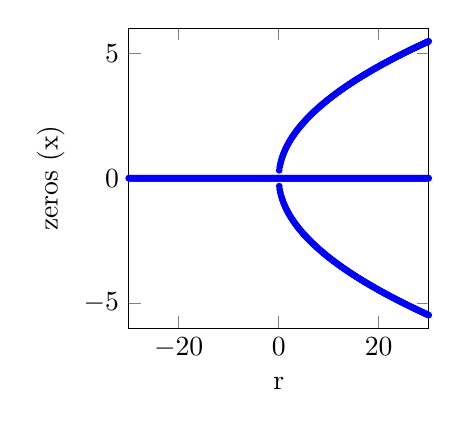
\begin{tikzpicture}

\begin{axis}[%
width=1.5in,
height=1.5in,
scale only axis,
xmin=-30,
xmax=30,
xlabel={r},
ymin=-6,
ymax=6,
ylabel={zeros (x)}
]
\addplot [color=blue,only marks,mark=*,mark size={1},forget plot]
  table[row sep=crcr]{%
-30	0\\
};
\addplot [color=blue,only marks,mark=*,mark size={1},forget plot]
  table[row sep=crcr]{%
-29.9	0\\
};
\addplot [color=blue,only marks,mark=*,mark size={1},forget plot]
  table[row sep=crcr]{%
-29.8	0\\
};
\addplot [color=blue,only marks,mark=*,mark size={1},forget plot]
  table[row sep=crcr]{%
-29.7	0\\
};
\addplot [color=blue,only marks,mark=*,mark size={1},forget plot]
  table[row sep=crcr]{%
-29.6	0\\
};
\addplot [color=blue,only marks,mark=*,mark size={1},forget plot]
  table[row sep=crcr]{%
-29.5	0\\
};
\addplot [color=blue,only marks,mark=*,mark size={1},forget plot]
  table[row sep=crcr]{%
-29.4	0\\
};
\addplot [color=blue,only marks,mark=*,mark size={1},forget plot]
  table[row sep=crcr]{%
-29.3	0\\
};
\addplot [color=blue,only marks,mark=*,mark size={1},forget plot]
  table[row sep=crcr]{%
-29.2	0\\
};
\addplot [color=blue,only marks,mark=*,mark size={1},forget plot]
  table[row sep=crcr]{%
-29.1	0\\
};
\addplot [color=blue,only marks,mark=*,mark size={1},forget plot]
  table[row sep=crcr]{%
-29	0\\
};
\addplot [color=blue,only marks,mark=*,mark size={1},forget plot]
  table[row sep=crcr]{%
-28.9	0\\
};
\addplot [color=blue,only marks,mark=*,mark size={1},forget plot]
  table[row sep=crcr]{%
-28.8	0\\
};
\addplot [color=blue,only marks,mark=*,mark size={1},forget plot]
  table[row sep=crcr]{%
-28.7	0\\
};
\addplot [color=blue,only marks,mark=*,mark size={1},forget plot]
  table[row sep=crcr]{%
-28.6	0\\
};
\addplot [color=blue,only marks,mark=*,mark size={1},forget plot]
  table[row sep=crcr]{%
-28.5	0\\
};
\addplot [color=blue,only marks,mark=*,mark size={1},forget plot]
  table[row sep=crcr]{%
-28.4	0\\
};
\addplot [color=blue,only marks,mark=*,mark size={1},forget plot]
  table[row sep=crcr]{%
-28.3	0\\
};
\addplot [color=blue,only marks,mark=*,mark size={1},forget plot]
  table[row sep=crcr]{%
-28.2	0\\
};
\addplot [color=blue,only marks,mark=*,mark size={1},forget plot]
  table[row sep=crcr]{%
-28.1	0\\
};
\addplot [color=blue,only marks,mark=*,mark size={1},forget plot]
  table[row sep=crcr]{%
-28	0\\
};
\addplot [color=blue,only marks,mark=*,mark size={1},forget plot]
  table[row sep=crcr]{%
-27.9	0\\
};
\addplot [color=blue,only marks,mark=*,mark size={1},forget plot]
  table[row sep=crcr]{%
-27.8	0\\
};
\addplot [color=blue,only marks,mark=*,mark size={1},forget plot]
  table[row sep=crcr]{%
-27.7	0\\
};
\addplot [color=blue,only marks,mark=*,mark size={1},forget plot]
  table[row sep=crcr]{%
-27.6	0\\
};
\addplot [color=blue,only marks,mark=*,mark size={1},forget plot]
  table[row sep=crcr]{%
-27.5	0\\
};
\addplot [color=blue,only marks,mark=*,mark size={1},forget plot]
  table[row sep=crcr]{%
-27.4	0\\
};
\addplot [color=blue,only marks,mark=*,mark size={1},forget plot]
  table[row sep=crcr]{%
-27.3	0\\
};
\addplot [color=blue,only marks,mark=*,mark size={1},forget plot]
  table[row sep=crcr]{%
-27.2	0\\
};
\addplot [color=blue,only marks,mark=*,mark size={1},forget plot]
  table[row sep=crcr]{%
-27.1	0\\
};
\addplot [color=blue,only marks,mark=*,mark size={1},forget plot]
  table[row sep=crcr]{%
-27	0\\
};
\addplot [color=blue,only marks,mark=*,mark size={1},forget plot]
  table[row sep=crcr]{%
-26.9	0\\
};
\addplot [color=blue,only marks,mark=*,mark size={1},forget plot]
  table[row sep=crcr]{%
-26.8	0\\
};
\addplot [color=blue,only marks,mark=*,mark size={1},forget plot]
  table[row sep=crcr]{%
-26.7	0\\
};
\addplot [color=blue,only marks,mark=*,mark size={1},forget plot]
  table[row sep=crcr]{%
-26.6	0\\
};
\addplot [color=blue,only marks,mark=*,mark size={1},forget plot]
  table[row sep=crcr]{%
-26.5	0\\
};
\addplot [color=blue,only marks,mark=*,mark size={1},forget plot]
  table[row sep=crcr]{%
-26.4	0\\
};
\addplot [color=blue,only marks,mark=*,mark size={1},forget plot]
  table[row sep=crcr]{%
-26.3	0\\
};
\addplot [color=blue,only marks,mark=*,mark size={1},forget plot]
  table[row sep=crcr]{%
-26.2	0\\
};
\addplot [color=blue,only marks,mark=*,mark size={1},forget plot]
  table[row sep=crcr]{%
-26.1	0\\
};
\addplot [color=blue,only marks,mark=*,mark size={1},forget plot]
  table[row sep=crcr]{%
-26	0\\
};
\addplot [color=blue,only marks,mark=*,mark size={1},forget plot]
  table[row sep=crcr]{%
-25.9	0\\
};
\addplot [color=blue,only marks,mark=*,mark size={1},forget plot]
  table[row sep=crcr]{%
-25.8	0\\
};
\addplot [color=blue,only marks,mark=*,mark size={1},forget plot]
  table[row sep=crcr]{%
-25.7	0\\
};
\addplot [color=blue,only marks,mark=*,mark size={1},forget plot]
  table[row sep=crcr]{%
-25.6	0\\
};
\addplot [color=blue,only marks,mark=*,mark size={1},forget plot]
  table[row sep=crcr]{%
-25.5	0\\
};
\addplot [color=blue,only marks,mark=*,mark size={1},forget plot]
  table[row sep=crcr]{%
-25.4	0\\
};
\addplot [color=blue,only marks,mark=*,mark size={1},forget plot]
  table[row sep=crcr]{%
-25.3	0\\
};
\addplot [color=blue,only marks,mark=*,mark size={1},forget plot]
  table[row sep=crcr]{%
-25.2	0\\
};
\addplot [color=blue,only marks,mark=*,mark size={1},forget plot]
  table[row sep=crcr]{%
-25.1	0\\
};
\addplot [color=blue,only marks,mark=*,mark size={1},forget plot]
  table[row sep=crcr]{%
-25	0\\
};
\addplot [color=blue,only marks,mark=*,mark size={1},forget plot]
  table[row sep=crcr]{%
-24.9	0\\
};
\addplot [color=blue,only marks,mark=*,mark size={1},forget plot]
  table[row sep=crcr]{%
-24.8	0\\
};
\addplot [color=blue,only marks,mark=*,mark size={1},forget plot]
  table[row sep=crcr]{%
-24.7	0\\
};
\addplot [color=blue,only marks,mark=*,mark size={1},forget plot]
  table[row sep=crcr]{%
-24.6	0\\
};
\addplot [color=blue,only marks,mark=*,mark size={1},forget plot]
  table[row sep=crcr]{%
-24.5	0\\
};
\addplot [color=blue,only marks,mark=*,mark size={1},forget plot]
  table[row sep=crcr]{%
-24.4	0\\
};
\addplot [color=blue,only marks,mark=*,mark size={1},forget plot]
  table[row sep=crcr]{%
-24.3	0\\
};
\addplot [color=blue,only marks,mark=*,mark size={1},forget plot]
  table[row sep=crcr]{%
-24.2	0\\
};
\addplot [color=blue,only marks,mark=*,mark size={1},forget plot]
  table[row sep=crcr]{%
-24.1	0\\
};
\addplot [color=blue,only marks,mark=*,mark size={1},forget plot]
  table[row sep=crcr]{%
-24	0\\
};
\addplot [color=blue,only marks,mark=*,mark size={1},forget plot]
  table[row sep=crcr]{%
-23.9	0\\
};
\addplot [color=blue,only marks,mark=*,mark size={1},forget plot]
  table[row sep=crcr]{%
-23.8	0\\
};
\addplot [color=blue,only marks,mark=*,mark size={1},forget plot]
  table[row sep=crcr]{%
-23.7	0\\
};
\addplot [color=blue,only marks,mark=*,mark size={1},forget plot]
  table[row sep=crcr]{%
-23.6	0\\
};
\addplot [color=blue,only marks,mark=*,mark size={1},forget plot]
  table[row sep=crcr]{%
-23.5	0\\
};
\addplot [color=blue,only marks,mark=*,mark size={1},forget plot]
  table[row sep=crcr]{%
-23.4	0\\
};
\addplot [color=blue,only marks,mark=*,mark size={1},forget plot]
  table[row sep=crcr]{%
-23.3	0\\
};
\addplot [color=blue,only marks,mark=*,mark size={1},forget plot]
  table[row sep=crcr]{%
-23.2	0\\
};
\addplot [color=blue,only marks,mark=*,mark size={1},forget plot]
  table[row sep=crcr]{%
-23.1	0\\
};
\addplot [color=blue,only marks,mark=*,mark size={1},forget plot]
  table[row sep=crcr]{%
-23	0\\
};
\addplot [color=blue,only marks,mark=*,mark size={1},forget plot]
  table[row sep=crcr]{%
-22.9	0\\
};
\addplot [color=blue,only marks,mark=*,mark size={1},forget plot]
  table[row sep=crcr]{%
-22.8	0\\
};
\addplot [color=blue,only marks,mark=*,mark size={1},forget plot]
  table[row sep=crcr]{%
-22.7	0\\
};
\addplot [color=blue,only marks,mark=*,mark size={1},forget plot]
  table[row sep=crcr]{%
-22.6	0\\
};
\addplot [color=blue,only marks,mark=*,mark size={1},forget plot]
  table[row sep=crcr]{%
-22.5	0\\
};
\addplot [color=blue,only marks,mark=*,mark size={1},forget plot]
  table[row sep=crcr]{%
-22.4	0\\
};
\addplot [color=blue,only marks,mark=*,mark size={1},forget plot]
  table[row sep=crcr]{%
-22.3	0\\
};
\addplot [color=blue,only marks,mark=*,mark size={1},forget plot]
  table[row sep=crcr]{%
-22.2	0\\
};
\addplot [color=blue,only marks,mark=*,mark size={1},forget plot]
  table[row sep=crcr]{%
-22.1	0\\
};
\addplot [color=blue,only marks,mark=*,mark size={1},forget plot]
  table[row sep=crcr]{%
-22	0\\
};
\addplot [color=blue,only marks,mark=*,mark size={1},forget plot]
  table[row sep=crcr]{%
-21.9	0\\
};
\addplot [color=blue,only marks,mark=*,mark size={1},forget plot]
  table[row sep=crcr]{%
-21.8	0\\
};
\addplot [color=blue,only marks,mark=*,mark size={1},forget plot]
  table[row sep=crcr]{%
-21.7	0\\
};
\addplot [color=blue,only marks,mark=*,mark size={1},forget plot]
  table[row sep=crcr]{%
-21.6	0\\
};
\addplot [color=blue,only marks,mark=*,mark size={1},forget plot]
  table[row sep=crcr]{%
-21.5	0\\
};
\addplot [color=blue,only marks,mark=*,mark size={1},forget plot]
  table[row sep=crcr]{%
-21.4	0\\
};
\addplot [color=blue,only marks,mark=*,mark size={1},forget plot]
  table[row sep=crcr]{%
-21.3	0\\
};
\addplot [color=blue,only marks,mark=*,mark size={1},forget plot]
  table[row sep=crcr]{%
-21.2	0\\
};
\addplot [color=blue,only marks,mark=*,mark size={1},forget plot]
  table[row sep=crcr]{%
-21.1	0\\
};
\addplot [color=blue,only marks,mark=*,mark size={1},forget plot]
  table[row sep=crcr]{%
-21	0\\
};
\addplot [color=blue,only marks,mark=*,mark size={1},forget plot]
  table[row sep=crcr]{%
-20.9	0\\
};
\addplot [color=blue,only marks,mark=*,mark size={1},forget plot]
  table[row sep=crcr]{%
-20.8	0\\
};
\addplot [color=blue,only marks,mark=*,mark size={1},forget plot]
  table[row sep=crcr]{%
-20.7	0\\
};
\addplot [color=blue,only marks,mark=*,mark size={1},forget plot]
  table[row sep=crcr]{%
-20.6	0\\
};
\addplot [color=blue,only marks,mark=*,mark size={1},forget plot]
  table[row sep=crcr]{%
-20.5	0\\
};
\addplot [color=blue,only marks,mark=*,mark size={1},forget plot]
  table[row sep=crcr]{%
-20.4	0\\
};
\addplot [color=blue,only marks,mark=*,mark size={1},forget plot]
  table[row sep=crcr]{%
-20.3	0\\
};
\addplot [color=blue,only marks,mark=*,mark size={1},forget plot]
  table[row sep=crcr]{%
-20.2	0\\
};
\addplot [color=blue,only marks,mark=*,mark size={1},forget plot]
  table[row sep=crcr]{%
-20.1	0\\
};
\addplot [color=blue,only marks,mark=*,mark size={1},forget plot]
  table[row sep=crcr]{%
-20	0\\
};
\addplot [color=blue,only marks,mark=*,mark size={1},forget plot]
  table[row sep=crcr]{%
-19.9	0\\
};
\addplot [color=blue,only marks,mark=*,mark size={1},forget plot]
  table[row sep=crcr]{%
-19.8	0\\
};
\addplot [color=blue,only marks,mark=*,mark size={1},forget plot]
  table[row sep=crcr]{%
-19.7	0\\
};
\addplot [color=blue,only marks,mark=*,mark size={1},forget plot]
  table[row sep=crcr]{%
-19.6	0\\
};
\addplot [color=blue,only marks,mark=*,mark size={1},forget plot]
  table[row sep=crcr]{%
-19.5	0\\
};
\addplot [color=blue,only marks,mark=*,mark size={1},forget plot]
  table[row sep=crcr]{%
-19.4	0\\
};
\addplot [color=blue,only marks,mark=*,mark size={1},forget plot]
  table[row sep=crcr]{%
-19.3	0\\
};
\addplot [color=blue,only marks,mark=*,mark size={1},forget plot]
  table[row sep=crcr]{%
-19.2	0\\
};
\addplot [color=blue,only marks,mark=*,mark size={1},forget plot]
  table[row sep=crcr]{%
-19.1	0\\
};
\addplot [color=blue,only marks,mark=*,mark size={1},forget plot]
  table[row sep=crcr]{%
-19	0\\
};
\addplot [color=blue,only marks,mark=*,mark size={1},forget plot]
  table[row sep=crcr]{%
-18.9	0\\
};
\addplot [color=blue,only marks,mark=*,mark size={1},forget plot]
  table[row sep=crcr]{%
-18.8	0\\
};
\addplot [color=blue,only marks,mark=*,mark size={1},forget plot]
  table[row sep=crcr]{%
-18.7	0\\
};
\addplot [color=blue,only marks,mark=*,mark size={1},forget plot]
  table[row sep=crcr]{%
-18.6	0\\
};
\addplot [color=blue,only marks,mark=*,mark size={1},forget plot]
  table[row sep=crcr]{%
-18.5	0\\
};
\addplot [color=blue,only marks,mark=*,mark size={1},forget plot]
  table[row sep=crcr]{%
-18.4	0\\
};
\addplot [color=blue,only marks,mark=*,mark size={1},forget plot]
  table[row sep=crcr]{%
-18.3	0\\
};
\addplot [color=blue,only marks,mark=*,mark size={1},forget plot]
  table[row sep=crcr]{%
-18.2	0\\
};
\addplot [color=blue,only marks,mark=*,mark size={1},forget plot]
  table[row sep=crcr]{%
-18.1	0\\
};
\addplot [color=blue,only marks,mark=*,mark size={1},forget plot]
  table[row sep=crcr]{%
-18	0\\
};
\addplot [color=blue,only marks,mark=*,mark size={1},forget plot]
  table[row sep=crcr]{%
-17.9	0\\
};
\addplot [color=blue,only marks,mark=*,mark size={1},forget plot]
  table[row sep=crcr]{%
-17.8	0\\
};
\addplot [color=blue,only marks,mark=*,mark size={1},forget plot]
  table[row sep=crcr]{%
-17.7	0\\
};
\addplot [color=blue,only marks,mark=*,mark size={1},forget plot]
  table[row sep=crcr]{%
-17.6	0\\
};
\addplot [color=blue,only marks,mark=*,mark size={1},forget plot]
  table[row sep=crcr]{%
-17.5	0\\
};
\addplot [color=blue,only marks,mark=*,mark size={1},forget plot]
  table[row sep=crcr]{%
-17.4	0\\
};
\addplot [color=blue,only marks,mark=*,mark size={1},forget plot]
  table[row sep=crcr]{%
-17.3	0\\
};
\addplot [color=blue,only marks,mark=*,mark size={1},forget plot]
  table[row sep=crcr]{%
-17.2	0\\
};
\addplot [color=blue,only marks,mark=*,mark size={1},forget plot]
  table[row sep=crcr]{%
-17.1	0\\
};
\addplot [color=blue,only marks,mark=*,mark size={1},forget plot]
  table[row sep=crcr]{%
-17	0\\
};
\addplot [color=blue,only marks,mark=*,mark size={1},forget plot]
  table[row sep=crcr]{%
-16.9	0\\
};
\addplot [color=blue,only marks,mark=*,mark size={1},forget plot]
  table[row sep=crcr]{%
-16.8	0\\
};
\addplot [color=blue,only marks,mark=*,mark size={1},forget plot]
  table[row sep=crcr]{%
-16.7	0\\
};
\addplot [color=blue,only marks,mark=*,mark size={1},forget plot]
  table[row sep=crcr]{%
-16.6	0\\
};
\addplot [color=blue,only marks,mark=*,mark size={1},forget plot]
  table[row sep=crcr]{%
-16.5	0\\
};
\addplot [color=blue,only marks,mark=*,mark size={1},forget plot]
  table[row sep=crcr]{%
-16.4	0\\
};
\addplot [color=blue,only marks,mark=*,mark size={1},forget plot]
  table[row sep=crcr]{%
-16.3	0\\
};
\addplot [color=blue,only marks,mark=*,mark size={1},forget plot]
  table[row sep=crcr]{%
-16.2	0\\
};
\addplot [color=blue,only marks,mark=*,mark size={1},forget plot]
  table[row sep=crcr]{%
-16.1	0\\
};
\addplot [color=blue,only marks,mark=*,mark size={1},forget plot]
  table[row sep=crcr]{%
-16	0\\
};
\addplot [color=blue,only marks,mark=*,mark size={1},forget plot]
  table[row sep=crcr]{%
-15.9	0\\
};
\addplot [color=blue,only marks,mark=*,mark size={1},forget plot]
  table[row sep=crcr]{%
-15.8	0\\
};
\addplot [color=blue,only marks,mark=*,mark size={1},forget plot]
  table[row sep=crcr]{%
-15.7	0\\
};
\addplot [color=blue,only marks,mark=*,mark size={1},forget plot]
  table[row sep=crcr]{%
-15.6	0\\
};
\addplot [color=blue,only marks,mark=*,mark size={1},forget plot]
  table[row sep=crcr]{%
-15.5	0\\
};
\addplot [color=blue,only marks,mark=*,mark size={1},forget plot]
  table[row sep=crcr]{%
-15.4	0\\
};
\addplot [color=blue,only marks,mark=*,mark size={1},forget plot]
  table[row sep=crcr]{%
-15.3	0\\
};
\addplot [color=blue,only marks,mark=*,mark size={1},forget plot]
  table[row sep=crcr]{%
-15.2	0\\
};
\addplot [color=blue,only marks,mark=*,mark size={1},forget plot]
  table[row sep=crcr]{%
-15.1	0\\
};
\addplot [color=blue,only marks,mark=*,mark size={1},forget plot]
  table[row sep=crcr]{%
-15	0\\
};
\addplot [color=blue,only marks,mark=*,mark size={1},forget plot]
  table[row sep=crcr]{%
-14.9	0\\
};
\addplot [color=blue,only marks,mark=*,mark size={1},forget plot]
  table[row sep=crcr]{%
-14.8	0\\
};
\addplot [color=blue,only marks,mark=*,mark size={1},forget plot]
  table[row sep=crcr]{%
-14.7	0\\
};
\addplot [color=blue,only marks,mark=*,mark size={1},forget plot]
  table[row sep=crcr]{%
-14.6	0\\
};
\addplot [color=blue,only marks,mark=*,mark size={1},forget plot]
  table[row sep=crcr]{%
-14.5	0\\
};
\addplot [color=blue,only marks,mark=*,mark size={1},forget plot]
  table[row sep=crcr]{%
-14.4	0\\
};
\addplot [color=blue,only marks,mark=*,mark size={1},forget plot]
  table[row sep=crcr]{%
-14.3	0\\
};
\addplot [color=blue,only marks,mark=*,mark size={1},forget plot]
  table[row sep=crcr]{%
-14.2	0\\
};
\addplot [color=blue,only marks,mark=*,mark size={1},forget plot]
  table[row sep=crcr]{%
-14.1	0\\
};
\addplot [color=blue,only marks,mark=*,mark size={1},forget plot]
  table[row sep=crcr]{%
-14	0\\
};
\addplot [color=blue,only marks,mark=*,mark size={1},forget plot]
  table[row sep=crcr]{%
-13.9	0\\
};
\addplot [color=blue,only marks,mark=*,mark size={1},forget plot]
  table[row sep=crcr]{%
-13.8	0\\
};
\addplot [color=blue,only marks,mark=*,mark size={1},forget plot]
  table[row sep=crcr]{%
-13.7	0\\
};
\addplot [color=blue,only marks,mark=*,mark size={1},forget plot]
  table[row sep=crcr]{%
-13.6	0\\
};
\addplot [color=blue,only marks,mark=*,mark size={1},forget plot]
  table[row sep=crcr]{%
-13.5	0\\
};
\addplot [color=blue,only marks,mark=*,mark size={1},forget plot]
  table[row sep=crcr]{%
-13.4	0\\
};
\addplot [color=blue,only marks,mark=*,mark size={1},forget plot]
  table[row sep=crcr]{%
-13.3	0\\
};
\addplot [color=blue,only marks,mark=*,mark size={1},forget plot]
  table[row sep=crcr]{%
-13.2	0\\
};
\addplot [color=blue,only marks,mark=*,mark size={1},forget plot]
  table[row sep=crcr]{%
-13.1	0\\
};
\addplot [color=blue,only marks,mark=*,mark size={1},forget plot]
  table[row sep=crcr]{%
-13	0\\
};
\addplot [color=blue,only marks,mark=*,mark size={1},forget plot]
  table[row sep=crcr]{%
-12.9	0\\
};
\addplot [color=blue,only marks,mark=*,mark size={1},forget plot]
  table[row sep=crcr]{%
-12.8	0\\
};
\addplot [color=blue,only marks,mark=*,mark size={1},forget plot]
  table[row sep=crcr]{%
-12.7	0\\
};
\addplot [color=blue,only marks,mark=*,mark size={1},forget plot]
  table[row sep=crcr]{%
-12.6	0\\
};
\addplot [color=blue,only marks,mark=*,mark size={1},forget plot]
  table[row sep=crcr]{%
-12.5	0\\
};
\addplot [color=blue,only marks,mark=*,mark size={1},forget plot]
  table[row sep=crcr]{%
-12.4	0\\
};
\addplot [color=blue,only marks,mark=*,mark size={1},forget plot]
  table[row sep=crcr]{%
-12.3	0\\
};
\addplot [color=blue,only marks,mark=*,mark size={1},forget plot]
  table[row sep=crcr]{%
-12.2	0\\
};
\addplot [color=blue,only marks,mark=*,mark size={1},forget plot]
  table[row sep=crcr]{%
-12.1	0\\
};
\addplot [color=blue,only marks,mark=*,mark size={1},forget plot]
  table[row sep=crcr]{%
-12	0\\
};
\addplot [color=blue,only marks,mark=*,mark size={1},forget plot]
  table[row sep=crcr]{%
-11.9	0\\
};
\addplot [color=blue,only marks,mark=*,mark size={1},forget plot]
  table[row sep=crcr]{%
-11.8	0\\
};
\addplot [color=blue,only marks,mark=*,mark size={1},forget plot]
  table[row sep=crcr]{%
-11.7	0\\
};
\addplot [color=blue,only marks,mark=*,mark size={1},forget plot]
  table[row sep=crcr]{%
-11.6	0\\
};
\addplot [color=blue,only marks,mark=*,mark size={1},forget plot]
  table[row sep=crcr]{%
-11.5	0\\
};
\addplot [color=blue,only marks,mark=*,mark size={1},forget plot]
  table[row sep=crcr]{%
-11.4	0\\
};
\addplot [color=blue,only marks,mark=*,mark size={1},forget plot]
  table[row sep=crcr]{%
-11.3	0\\
};
\addplot [color=blue,only marks,mark=*,mark size={1},forget plot]
  table[row sep=crcr]{%
-11.2	0\\
};
\addplot [color=blue,only marks,mark=*,mark size={1},forget plot]
  table[row sep=crcr]{%
-11.1	0\\
};
\addplot [color=blue,only marks,mark=*,mark size={1},forget plot]
  table[row sep=crcr]{%
-11	0\\
};
\addplot [color=blue,only marks,mark=*,mark size={1},forget plot]
  table[row sep=crcr]{%
-10.9	0\\
};
\addplot [color=blue,only marks,mark=*,mark size={1},forget plot]
  table[row sep=crcr]{%
-10.8	0\\
};
\addplot [color=blue,only marks,mark=*,mark size={1},forget plot]
  table[row sep=crcr]{%
-10.7	0\\
};
\addplot [color=blue,only marks,mark=*,mark size={1},forget plot]
  table[row sep=crcr]{%
-10.6	0\\
};
\addplot [color=blue,only marks,mark=*,mark size={1},forget plot]
  table[row sep=crcr]{%
-10.5	0\\
};
\addplot [color=blue,only marks,mark=*,mark size={1},forget plot]
  table[row sep=crcr]{%
-10.4	0\\
};
\addplot [color=blue,only marks,mark=*,mark size={1},forget plot]
  table[row sep=crcr]{%
-10.3	0\\
};
\addplot [color=blue,only marks,mark=*,mark size={1},forget plot]
  table[row sep=crcr]{%
-10.2	0\\
};
\addplot [color=blue,only marks,mark=*,mark size={1},forget plot]
  table[row sep=crcr]{%
-10.1	0\\
};
\addplot [color=blue,only marks,mark=*,mark size={1},forget plot]
  table[row sep=crcr]{%
-10	0\\
};
\addplot [color=blue,only marks,mark=*,mark size={1},forget plot]
  table[row sep=crcr]{%
-9.9	0\\
};
\addplot [color=blue,only marks,mark=*,mark size={1},forget plot]
  table[row sep=crcr]{%
-9.8	0\\
};
\addplot [color=blue,only marks,mark=*,mark size={1},forget plot]
  table[row sep=crcr]{%
-9.7	0\\
};
\addplot [color=blue,only marks,mark=*,mark size={1},forget plot]
  table[row sep=crcr]{%
-9.6	0\\
};
\addplot [color=blue,only marks,mark=*,mark size={1},forget plot]
  table[row sep=crcr]{%
-9.5	0\\
};
\addplot [color=blue,only marks,mark=*,mark size={1},forget plot]
  table[row sep=crcr]{%
-9.4	0\\
};
\addplot [color=blue,only marks,mark=*,mark size={1},forget plot]
  table[row sep=crcr]{%
-9.3	0\\
};
\addplot [color=blue,only marks,mark=*,mark size={1},forget plot]
  table[row sep=crcr]{%
-9.2	0\\
};
\addplot [color=blue,only marks,mark=*,mark size={1},forget plot]
  table[row sep=crcr]{%
-9.1	0\\
};
\addplot [color=blue,only marks,mark=*,mark size={1},forget plot]
  table[row sep=crcr]{%
-9	0\\
};
\addplot [color=blue,only marks,mark=*,mark size={1},forget plot]
  table[row sep=crcr]{%
-8.9	0\\
};
\addplot [color=blue,only marks,mark=*,mark size={1},forget plot]
  table[row sep=crcr]{%
-8.8	0\\
};
\addplot [color=blue,only marks,mark=*,mark size={1},forget plot]
  table[row sep=crcr]{%
-8.7	0\\
};
\addplot [color=blue,only marks,mark=*,mark size={1},forget plot]
  table[row sep=crcr]{%
-8.6	0\\
};
\addplot [color=blue,only marks,mark=*,mark size={1},forget plot]
  table[row sep=crcr]{%
-8.5	0\\
};
\addplot [color=blue,only marks,mark=*,mark size={1},forget plot]
  table[row sep=crcr]{%
-8.4	0\\
};
\addplot [color=blue,only marks,mark=*,mark size={1},forget plot]
  table[row sep=crcr]{%
-8.3	0\\
};
\addplot [color=blue,only marks,mark=*,mark size={1},forget plot]
  table[row sep=crcr]{%
-8.2	0\\
};
\addplot [color=blue,only marks,mark=*,mark size={1},forget plot]
  table[row sep=crcr]{%
-8.1	0\\
};
\addplot [color=blue,only marks,mark=*,mark size={1},forget plot]
  table[row sep=crcr]{%
-8	0\\
};
\addplot [color=blue,only marks,mark=*,mark size={1},forget plot]
  table[row sep=crcr]{%
-7.9	0\\
};
\addplot [color=blue,only marks,mark=*,mark size={1},forget plot]
  table[row sep=crcr]{%
-7.8	0\\
};
\addplot [color=blue,only marks,mark=*,mark size={1},forget plot]
  table[row sep=crcr]{%
-7.7	0\\
};
\addplot [color=blue,only marks,mark=*,mark size={1},forget plot]
  table[row sep=crcr]{%
-7.6	0\\
};
\addplot [color=blue,only marks,mark=*,mark size={1},forget plot]
  table[row sep=crcr]{%
-7.5	0\\
};
\addplot [color=blue,only marks,mark=*,mark size={1},forget plot]
  table[row sep=crcr]{%
-7.4	0\\
};
\addplot [color=blue,only marks,mark=*,mark size={1},forget plot]
  table[row sep=crcr]{%
-7.3	0\\
};
\addplot [color=blue,only marks,mark=*,mark size={1},forget plot]
  table[row sep=crcr]{%
-7.2	0\\
};
\addplot [color=blue,only marks,mark=*,mark size={1},forget plot]
  table[row sep=crcr]{%
-7.1	0\\
};
\addplot [color=blue,only marks,mark=*,mark size={1},forget plot]
  table[row sep=crcr]{%
-7	0\\
};
\addplot [color=blue,only marks,mark=*,mark size={1},forget plot]
  table[row sep=crcr]{%
-6.9	0\\
};
\addplot [color=blue,only marks,mark=*,mark size={1},forget plot]
  table[row sep=crcr]{%
-6.8	0\\
};
\addplot [color=blue,only marks,mark=*,mark size={1},forget plot]
  table[row sep=crcr]{%
-6.7	0\\
};
\addplot [color=blue,only marks,mark=*,mark size={1},forget plot]
  table[row sep=crcr]{%
-6.6	0\\
};
\addplot [color=blue,only marks,mark=*,mark size={1},forget plot]
  table[row sep=crcr]{%
-6.5	0\\
};
\addplot [color=blue,only marks,mark=*,mark size={1},forget plot]
  table[row sep=crcr]{%
-6.4	0\\
};
\addplot [color=blue,only marks,mark=*,mark size={1},forget plot]
  table[row sep=crcr]{%
-6.3	0\\
};
\addplot [color=blue,only marks,mark=*,mark size={1},forget plot]
  table[row sep=crcr]{%
-6.2	0\\
};
\addplot [color=blue,only marks,mark=*,mark size={1},forget plot]
  table[row sep=crcr]{%
-6.1	0\\
};
\addplot [color=blue,only marks,mark=*,mark size={1},forget plot]
  table[row sep=crcr]{%
-6	0\\
};
\addplot [color=blue,only marks,mark=*,mark size={1},forget plot]
  table[row sep=crcr]{%
-5.9	0\\
};
\addplot [color=blue,only marks,mark=*,mark size={1},forget plot]
  table[row sep=crcr]{%
-5.8	0\\
};
\addplot [color=blue,only marks,mark=*,mark size={1},forget plot]
  table[row sep=crcr]{%
-5.7	0\\
};
\addplot [color=blue,only marks,mark=*,mark size={1},forget plot]
  table[row sep=crcr]{%
-5.6	0\\
};
\addplot [color=blue,only marks,mark=*,mark size={1},forget plot]
  table[row sep=crcr]{%
-5.5	0\\
};
\addplot [color=blue,only marks,mark=*,mark size={1},forget plot]
  table[row sep=crcr]{%
-5.4	0\\
};
\addplot [color=blue,only marks,mark=*,mark size={1},forget plot]
  table[row sep=crcr]{%
-5.3	0\\
};
\addplot [color=blue,only marks,mark=*,mark size={1},forget plot]
  table[row sep=crcr]{%
-5.2	0\\
};
\addplot [color=blue,only marks,mark=*,mark size={1},forget plot]
  table[row sep=crcr]{%
-5.1	0\\
};
\addplot [color=blue,only marks,mark=*,mark size={1},forget plot]
  table[row sep=crcr]{%
-5	0\\
};
\addplot [color=blue,only marks,mark=*,mark size={1},forget plot]
  table[row sep=crcr]{%
-4.9	0\\
};
\addplot [color=blue,only marks,mark=*,mark size={1},forget plot]
  table[row sep=crcr]{%
-4.8	0\\
};
\addplot [color=blue,only marks,mark=*,mark size={1},forget plot]
  table[row sep=crcr]{%
-4.7	0\\
};
\addplot [color=blue,only marks,mark=*,mark size={1},forget plot]
  table[row sep=crcr]{%
-4.6	0\\
};
\addplot [color=blue,only marks,mark=*,mark size={1},forget plot]
  table[row sep=crcr]{%
-4.5	0\\
};
\addplot [color=blue,only marks,mark=*,mark size={1},forget plot]
  table[row sep=crcr]{%
-4.4	0\\
};
\addplot [color=blue,only marks,mark=*,mark size={1},forget plot]
  table[row sep=crcr]{%
-4.3	0\\
};
\addplot [color=blue,only marks,mark=*,mark size={1},forget plot]
  table[row sep=crcr]{%
-4.2	0\\
};
\addplot [color=blue,only marks,mark=*,mark size={1},forget plot]
  table[row sep=crcr]{%
-4.1	0\\
};
\addplot [color=blue,only marks,mark=*,mark size={1},forget plot]
  table[row sep=crcr]{%
-4	0\\
};
\addplot [color=blue,only marks,mark=*,mark size={1},forget plot]
  table[row sep=crcr]{%
-3.9	0\\
};
\addplot [color=blue,only marks,mark=*,mark size={1},forget plot]
  table[row sep=crcr]{%
-3.8	0\\
};
\addplot [color=blue,only marks,mark=*,mark size={1},forget plot]
  table[row sep=crcr]{%
-3.7	0\\
};
\addplot [color=blue,only marks,mark=*,mark size={1},forget plot]
  table[row sep=crcr]{%
-3.6	0\\
};
\addplot [color=blue,only marks,mark=*,mark size={1},forget plot]
  table[row sep=crcr]{%
-3.5	0\\
};
\addplot [color=blue,only marks,mark=*,mark size={1},forget plot]
  table[row sep=crcr]{%
-3.4	0\\
};
\addplot [color=blue,only marks,mark=*,mark size={1},forget plot]
  table[row sep=crcr]{%
-3.3	0\\
};
\addplot [color=blue,only marks,mark=*,mark size={1},forget plot]
  table[row sep=crcr]{%
-3.2	0\\
};
\addplot [color=blue,only marks,mark=*,mark size={1},forget plot]
  table[row sep=crcr]{%
-3.1	0\\
};
\addplot [color=blue,only marks,mark=*,mark size={1},forget plot]
  table[row sep=crcr]{%
-3	0\\
};
\addplot [color=blue,only marks,mark=*,mark size={1},forget plot]
  table[row sep=crcr]{%
-2.9	0\\
};
\addplot [color=blue,only marks,mark=*,mark size={1},forget plot]
  table[row sep=crcr]{%
-2.8	0\\
};
\addplot [color=blue,only marks,mark=*,mark size={1},forget plot]
  table[row sep=crcr]{%
-2.7	0\\
};
\addplot [color=blue,only marks,mark=*,mark size={1},forget plot]
  table[row sep=crcr]{%
-2.6	0\\
};
\addplot [color=blue,only marks,mark=*,mark size={1},forget plot]
  table[row sep=crcr]{%
-2.5	0\\
};
\addplot [color=blue,only marks,mark=*,mark size={1},forget plot]
  table[row sep=crcr]{%
-2.4	0\\
};
\addplot [color=blue,only marks,mark=*,mark size={1},forget plot]
  table[row sep=crcr]{%
-2.3	0\\
};
\addplot [color=blue,only marks,mark=*,mark size={1},forget plot]
  table[row sep=crcr]{%
-2.2	0\\
};
\addplot [color=blue,only marks,mark=*,mark size={1},forget plot]
  table[row sep=crcr]{%
-2.1	0\\
};
\addplot [color=blue,only marks,mark=*,mark size={1},forget plot]
  table[row sep=crcr]{%
-2	0\\
};
\addplot [color=blue,only marks,mark=*,mark size={1},forget plot]
  table[row sep=crcr]{%
-1.9	0\\
};
\addplot [color=blue,only marks,mark=*,mark size={1},forget plot]
  table[row sep=crcr]{%
-1.8	0\\
};
\addplot [color=blue,only marks,mark=*,mark size={1},forget plot]
  table[row sep=crcr]{%
-1.7	0\\
};
\addplot [color=blue,only marks,mark=*,mark size={1},forget plot]
  table[row sep=crcr]{%
-1.6	0\\
};
\addplot [color=blue,only marks,mark=*,mark size={1},forget plot]
  table[row sep=crcr]{%
-1.5	0\\
};
\addplot [color=blue,only marks,mark=*,mark size={1},forget plot]
  table[row sep=crcr]{%
-1.4	0\\
};
\addplot [color=blue,only marks,mark=*,mark size={1},forget plot]
  table[row sep=crcr]{%
-1.3	0\\
};
\addplot [color=blue,only marks,mark=*,mark size={1},forget plot]
  table[row sep=crcr]{%
-1.2	0\\
};
\addplot [color=blue,only marks,mark=*,mark size={1},forget plot]
  table[row sep=crcr]{%
-1.1	0\\
};
\addplot [color=blue,only marks,mark=*,mark size={1},forget plot]
  table[row sep=crcr]{%
-1	0\\
};
\addplot [color=blue,only marks,mark=*,mark size={1},forget plot]
  table[row sep=crcr]{%
-0.899999999999999	0\\
};
\addplot [color=blue,only marks,mark=*,mark size={1},forget plot]
  table[row sep=crcr]{%
-0.799999999999997	0\\
};
\addplot [color=blue,only marks,mark=*,mark size={1},forget plot]
  table[row sep=crcr]{%
-0.699999999999999	0\\
};
\addplot [color=blue,only marks,mark=*,mark size={1},forget plot]
  table[row sep=crcr]{%
-0.599999999999998	0\\
};
\addplot [color=blue,only marks,mark=*,mark size={1},forget plot]
  table[row sep=crcr]{%
-0.5	0\\
};
\addplot [color=blue,only marks,mark=*,mark size={1},forget plot]
  table[row sep=crcr]{%
-0.399999999999999	0\\
};
\addplot [color=blue,only marks,mark=*,mark size={1},forget plot]
  table[row sep=crcr]{%
-0.299999999999997	0\\
};
\addplot [color=blue,only marks,mark=*,mark size={1},forget plot]
  table[row sep=crcr]{%
-0.199999999999999	0\\
};
\addplot [color=blue,only marks,mark=*,mark size={1},forget plot]
  table[row sep=crcr]{%
-0.0999999999999979	0\\
};
\addplot [color=blue,only marks,mark=*,mark size={1},forget plot]
  table[row sep=crcr]{%
0	0\\
};
\addplot [color=blue,only marks,mark=*,mark size={1},forget plot]
  table[row sep=crcr]{%
0	0\\
};
\addplot [color=blue,only marks,mark=*,mark size={1},forget plot]
  table[row sep=crcr]{%
0	0\\
};
\addplot [color=blue,only marks,mark=*,mark size={1},forget plot]
  table[row sep=crcr]{%
0.100000000000001	0\\
};
\addplot [color=blue,only marks,mark=*,mark size={1},forget plot]
  table[row sep=crcr]{%
0.100000000000001	0.31622776601684\\
};
\addplot [color=blue,only marks,mark=*,mark size={1},forget plot]
  table[row sep=crcr]{%
0.100000000000001	-0.31622776601684\\
};
\addplot [color=blue,only marks,mark=*,mark size={1},forget plot]
  table[row sep=crcr]{%
0.200000000000003	0\\
};
\addplot [color=blue,only marks,mark=*,mark size={1},forget plot]
  table[row sep=crcr]{%
0.200000000000003	0.447213595499961\\
};
\addplot [color=blue,only marks,mark=*,mark size={1},forget plot]
  table[row sep=crcr]{%
0.200000000000003	-0.447213595499961\\
};
\addplot [color=blue,only marks,mark=*,mark size={1},forget plot]
  table[row sep=crcr]{%
0.300000000000001	0\\
};
\addplot [color=blue,only marks,mark=*,mark size={1},forget plot]
  table[row sep=crcr]{%
0.300000000000001	0.547722557505167\\
};
\addplot [color=blue,only marks,mark=*,mark size={1},forget plot]
  table[row sep=crcr]{%
0.300000000000001	-0.547722557505167\\
};
\addplot [color=blue,only marks,mark=*,mark size={1},forget plot]
  table[row sep=crcr]{%
0.400000000000002	0\\
};
\addplot [color=blue,only marks,mark=*,mark size={1},forget plot]
  table[row sep=crcr]{%
0.400000000000002	0.632455532033678\\
};
\addplot [color=blue,only marks,mark=*,mark size={1},forget plot]
  table[row sep=crcr]{%
0.400000000000002	-0.632455532033677\\
};
\addplot [color=blue,only marks,mark=*,mark size={1},forget plot]
  table[row sep=crcr]{%
0.5	0\\
};
\addplot [color=blue,only marks,mark=*,mark size={1},forget plot]
  table[row sep=crcr]{%
0.5	0.707106781186548\\
};
\addplot [color=blue,only marks,mark=*,mark size={1},forget plot]
  table[row sep=crcr]{%
0.5	-0.707106781186547\\
};
\addplot [color=blue,only marks,mark=*,mark size={1},forget plot]
  table[row sep=crcr]{%
0.600000000000001	0\\
};
\addplot [color=blue,only marks,mark=*,mark size={1},forget plot]
  table[row sep=crcr]{%
0.600000000000001	0.774596669241484\\
};
\addplot [color=blue,only marks,mark=*,mark size={1},forget plot]
  table[row sep=crcr]{%
0.600000000000001	-0.774596669241484\\
};
\addplot [color=blue,only marks,mark=*,mark size={1},forget plot]
  table[row sep=crcr]{%
0.700000000000003	0\\
};
\addplot [color=blue,only marks,mark=*,mark size={1},forget plot]
  table[row sep=crcr]{%
0.700000000000003	0.836660026534077\\
};
\addplot [color=blue,only marks,mark=*,mark size={1},forget plot]
  table[row sep=crcr]{%
0.700000000000003	-0.836660026534077\\
};
\addplot [color=blue,only marks,mark=*,mark size={1},forget plot]
  table[row sep=crcr]{%
0.800000000000001	0\\
};
\addplot [color=blue,only marks,mark=*,mark size={1},forget plot]
  table[row sep=crcr]{%
0.800000000000001	0.894427190999916\\
};
\addplot [color=blue,only marks,mark=*,mark size={1},forget plot]
  table[row sep=crcr]{%
0.800000000000001	-0.894427190999916\\
};
\addplot [color=blue,only marks,mark=*,mark size={1},forget plot]
  table[row sep=crcr]{%
0.900000000000002	0\\
};
\addplot [color=blue,only marks,mark=*,mark size={1},forget plot]
  table[row sep=crcr]{%
0.900000000000002	0.948683298050515\\
};
\addplot [color=blue,only marks,mark=*,mark size={1},forget plot]
  table[row sep=crcr]{%
0.900000000000002	-0.948683298050515\\
};
\addplot [color=blue,only marks,mark=*,mark size={1},forget plot]
  table[row sep=crcr]{%
1	0\\
};
\addplot [color=blue,only marks,mark=*,mark size={1},forget plot]
  table[row sep=crcr]{%
1	-1\\
};
\addplot [color=blue,only marks,mark=*,mark size={1},forget plot]
  table[row sep=crcr]{%
1	1\\
};
\addplot [color=blue,only marks,mark=*,mark size={1},forget plot]
  table[row sep=crcr]{%
1.1	0\\
};
\addplot [color=blue,only marks,mark=*,mark size={1},forget plot]
  table[row sep=crcr]{%
1.1	1.04880884817015\\
};
\addplot [color=blue,only marks,mark=*,mark size={1},forget plot]
  table[row sep=crcr]{%
1.1	-1.04880884817015\\
};
\addplot [color=blue,only marks,mark=*,mark size={1},forget plot]
  table[row sep=crcr]{%
1.2	0\\
};
\addplot [color=blue,only marks,mark=*,mark size={1},forget plot]
  table[row sep=crcr]{%
1.2	1.09544511501033\\
};
\addplot [color=blue,only marks,mark=*,mark size={1},forget plot]
  table[row sep=crcr]{%
1.2	-1.09544511501033\\
};
\addplot [color=blue,only marks,mark=*,mark size={1},forget plot]
  table[row sep=crcr]{%
1.3	0\\
};
\addplot [color=blue,only marks,mark=*,mark size={1},forget plot]
  table[row sep=crcr]{%
1.3	1.14017542509914\\
};
\addplot [color=blue,only marks,mark=*,mark size={1},forget plot]
  table[row sep=crcr]{%
1.3	-1.14017542509914\\
};
\addplot [color=blue,only marks,mark=*,mark size={1},forget plot]
  table[row sep=crcr]{%
1.4	0\\
};
\addplot [color=blue,only marks,mark=*,mark size={1},forget plot]
  table[row sep=crcr]{%
1.4	1.18321595661992\\
};
\addplot [color=blue,only marks,mark=*,mark size={1},forget plot]
  table[row sep=crcr]{%
1.4	-1.18321595661992\\
};
\addplot [color=blue,only marks,mark=*,mark size={1},forget plot]
  table[row sep=crcr]{%
1.5	0\\
};
\addplot [color=blue,only marks,mark=*,mark size={1},forget plot]
  table[row sep=crcr]{%
1.5	1.22474487139159\\
};
\addplot [color=blue,only marks,mark=*,mark size={1},forget plot]
  table[row sep=crcr]{%
1.5	-1.22474487139159\\
};
\addplot [color=blue,only marks,mark=*,mark size={1},forget plot]
  table[row sep=crcr]{%
1.6	0\\
};
\addplot [color=blue,only marks,mark=*,mark size={1},forget plot]
  table[row sep=crcr]{%
1.6	1.26491106406735\\
};
\addplot [color=blue,only marks,mark=*,mark size={1},forget plot]
  table[row sep=crcr]{%
1.6	-1.26491106406735\\
};
\addplot [color=blue,only marks,mark=*,mark size={1},forget plot]
  table[row sep=crcr]{%
1.7	0\\
};
\addplot [color=blue,only marks,mark=*,mark size={1},forget plot]
  table[row sep=crcr]{%
1.7	1.30384048104053\\
};
\addplot [color=blue,only marks,mark=*,mark size={1},forget plot]
  table[row sep=crcr]{%
1.7	-1.30384048104053\\
};
\addplot [color=blue,only marks,mark=*,mark size={1},forget plot]
  table[row sep=crcr]{%
1.8	0\\
};
\addplot [color=blue,only marks,mark=*,mark size={1},forget plot]
  table[row sep=crcr]{%
1.8	1.34164078649987\\
};
\addplot [color=blue,only marks,mark=*,mark size={1},forget plot]
  table[row sep=crcr]{%
1.8	-1.34164078649987\\
};
\addplot [color=blue,only marks,mark=*,mark size={1},forget plot]
  table[row sep=crcr]{%
1.9	0\\
};
\addplot [color=blue,only marks,mark=*,mark size={1},forget plot]
  table[row sep=crcr]{%
1.9	1.37840487520902\\
};
\addplot [color=blue,only marks,mark=*,mark size={1},forget plot]
  table[row sep=crcr]{%
1.9	-1.37840487520902\\
};
\addplot [color=blue,only marks,mark=*,mark size={1},forget plot]
  table[row sep=crcr]{%
2	0\\
};
\addplot [color=blue,only marks,mark=*,mark size={1},forget plot]
  table[row sep=crcr]{%
2	1.4142135623731\\
};
\addplot [color=blue,only marks,mark=*,mark size={1},forget plot]
  table[row sep=crcr]{%
2	-1.41421356237309\\
};
\addplot [color=blue,only marks,mark=*,mark size={1},forget plot]
  table[row sep=crcr]{%
2.1	0\\
};
\addplot [color=blue,only marks,mark=*,mark size={1},forget plot]
  table[row sep=crcr]{%
2.1	1.44913767461894\\
};
\addplot [color=blue,only marks,mark=*,mark size={1},forget plot]
  table[row sep=crcr]{%
2.1	-1.44913767461894\\
};
\addplot [color=blue,only marks,mark=*,mark size={1},forget plot]
  table[row sep=crcr]{%
2.2	0\\
};
\addplot [color=blue,only marks,mark=*,mark size={1},forget plot]
  table[row sep=crcr]{%
2.2	1.48323969741913\\
};
\addplot [color=blue,only marks,mark=*,mark size={1},forget plot]
  table[row sep=crcr]{%
2.2	-1.48323969741913\\
};
\addplot [color=blue,only marks,mark=*,mark size={1},forget plot]
  table[row sep=crcr]{%
2.3	0\\
};
\addplot [color=blue,only marks,mark=*,mark size={1},forget plot]
  table[row sep=crcr]{%
2.3	1.51657508881031\\
};
\addplot [color=blue,only marks,mark=*,mark size={1},forget plot]
  table[row sep=crcr]{%
2.3	-1.51657508881031\\
};
\addplot [color=blue,only marks,mark=*,mark size={1},forget plot]
  table[row sep=crcr]{%
2.4	0\\
};
\addplot [color=blue,only marks,mark=*,mark size={1},forget plot]
  table[row sep=crcr]{%
2.4	1.54919333848297\\
};
\addplot [color=blue,only marks,mark=*,mark size={1},forget plot]
  table[row sep=crcr]{%
2.4	-1.54919333848297\\
};
\addplot [color=blue,only marks,mark=*,mark size={1},forget plot]
  table[row sep=crcr]{%
2.5	0\\
};
\addplot [color=blue,only marks,mark=*,mark size={1},forget plot]
  table[row sep=crcr]{%
2.5	1.58113883008419\\
};
\addplot [color=blue,only marks,mark=*,mark size={1},forget plot]
  table[row sep=crcr]{%
2.5	-1.58113883008419\\
};
\addplot [color=blue,only marks,mark=*,mark size={1},forget plot]
  table[row sep=crcr]{%
2.6	0\\
};
\addplot [color=blue,only marks,mark=*,mark size={1},forget plot]
  table[row sep=crcr]{%
2.6	1.61245154965971\\
};
\addplot [color=blue,only marks,mark=*,mark size={1},forget plot]
  table[row sep=crcr]{%
2.6	-1.61245154965971\\
};
\addplot [color=blue,only marks,mark=*,mark size={1},forget plot]
  table[row sep=crcr]{%
2.7	0\\
};
\addplot [color=blue,only marks,mark=*,mark size={1},forget plot]
  table[row sep=crcr]{%
2.7	1.6431676725155\\
};
\addplot [color=blue,only marks,mark=*,mark size={1},forget plot]
  table[row sep=crcr]{%
2.7	-1.6431676725155\\
};
\addplot [color=blue,only marks,mark=*,mark size={1},forget plot]
  table[row sep=crcr]{%
2.8	0\\
};
\addplot [color=blue,only marks,mark=*,mark size={1},forget plot]
  table[row sep=crcr]{%
2.8	1.67332005306815\\
};
\addplot [color=blue,only marks,mark=*,mark size={1},forget plot]
  table[row sep=crcr]{%
2.8	-1.67332005306815\\
};
\addplot [color=blue,only marks,mark=*,mark size={1},forget plot]
  table[row sep=crcr]{%
2.9	0\\
};
\addplot [color=blue,only marks,mark=*,mark size={1},forget plot]
  table[row sep=crcr]{%
2.9	1.70293863659264\\
};
\addplot [color=blue,only marks,mark=*,mark size={1},forget plot]
  table[row sep=crcr]{%
2.9	-1.70293863659264\\
};
\addplot [color=blue,only marks,mark=*,mark size={1},forget plot]
  table[row sep=crcr]{%
3	0\\
};
\addplot [color=blue,only marks,mark=*,mark size={1},forget plot]
  table[row sep=crcr]{%
3	1.73205080756888\\
};
\addplot [color=blue,only marks,mark=*,mark size={1},forget plot]
  table[row sep=crcr]{%
3	-1.73205080756888\\
};
\addplot [color=blue,only marks,mark=*,mark size={1},forget plot]
  table[row sep=crcr]{%
3.1	0\\
};
\addplot [color=blue,only marks,mark=*,mark size={1},forget plot]
  table[row sep=crcr]{%
3.1	1.7606816861659\\
};
\addplot [color=blue,only marks,mark=*,mark size={1},forget plot]
  table[row sep=crcr]{%
3.1	-1.7606816861659\\
};
\addplot [color=blue,only marks,mark=*,mark size={1},forget plot]
  table[row sep=crcr]{%
3.2	0\\
};
\addplot [color=blue,only marks,mark=*,mark size={1},forget plot]
  table[row sep=crcr]{%
3.2	1.78885438199983\\
};
\addplot [color=blue,only marks,mark=*,mark size={1},forget plot]
  table[row sep=crcr]{%
3.2	-1.78885438199983\\
};
\addplot [color=blue,only marks,mark=*,mark size={1},forget plot]
  table[row sep=crcr]{%
3.3	0\\
};
\addplot [color=blue,only marks,mark=*,mark size={1},forget plot]
  table[row sep=crcr]{%
3.3	1.8165902124585\\
};
\addplot [color=blue,only marks,mark=*,mark size={1},forget plot]
  table[row sep=crcr]{%
3.3	-1.8165902124585\\
};
\addplot [color=blue,only marks,mark=*,mark size={1},forget plot]
  table[row sep=crcr]{%
3.4	0\\
};
\addplot [color=blue,only marks,mark=*,mark size={1},forget plot]
  table[row sep=crcr]{%
3.4	1.84390889145858\\
};
\addplot [color=blue,only marks,mark=*,mark size={1},forget plot]
  table[row sep=crcr]{%
3.4	-1.84390889145858\\
};
\addplot [color=blue,only marks,mark=*,mark size={1},forget plot]
  table[row sep=crcr]{%
3.5	0\\
};
\addplot [color=blue,only marks,mark=*,mark size={1},forget plot]
  table[row sep=crcr]{%
3.5	1.87082869338697\\
};
\addplot [color=blue,only marks,mark=*,mark size={1},forget plot]
  table[row sep=crcr]{%
3.5	-1.87082869338697\\
};
\addplot [color=blue,only marks,mark=*,mark size={1},forget plot]
  table[row sep=crcr]{%
3.6	0\\
};
\addplot [color=blue,only marks,mark=*,mark size={1},forget plot]
  table[row sep=crcr]{%
3.6	1.89736659610103\\
};
\addplot [color=blue,only marks,mark=*,mark size={1},forget plot]
  table[row sep=crcr]{%
3.6	-1.89736659610103\\
};
\addplot [color=blue,only marks,mark=*,mark size={1},forget plot]
  table[row sep=crcr]{%
3.7	0\\
};
\addplot [color=blue,only marks,mark=*,mark size={1},forget plot]
  table[row sep=crcr]{%
3.7	1.92353840616714\\
};
\addplot [color=blue,only marks,mark=*,mark size={1},forget plot]
  table[row sep=crcr]{%
3.7	-1.92353840616714\\
};
\addplot [color=blue,only marks,mark=*,mark size={1},forget plot]
  table[row sep=crcr]{%
3.8	0\\
};
\addplot [color=blue,only marks,mark=*,mark size={1},forget plot]
  table[row sep=crcr]{%
3.8	1.94935886896179\\
};
\addplot [color=blue,only marks,mark=*,mark size={1},forget plot]
  table[row sep=crcr]{%
3.8	-1.94935886896179\\
};
\addplot [color=blue,only marks,mark=*,mark size={1},forget plot]
  table[row sep=crcr]{%
3.9	0\\
};
\addplot [color=blue,only marks,mark=*,mark size={1},forget plot]
  table[row sep=crcr]{%
3.9	1.97484176581315\\
};
\addplot [color=blue,only marks,mark=*,mark size={1},forget plot]
  table[row sep=crcr]{%
3.9	-1.97484176581315\\
};
\addplot [color=blue,only marks,mark=*,mark size={1},forget plot]
  table[row sep=crcr]{%
4	0\\
};
\addplot [color=blue,only marks,mark=*,mark size={1},forget plot]
  table[row sep=crcr]{%
4	2\\
};
\addplot [color=blue,only marks,mark=*,mark size={1},forget plot]
  table[row sep=crcr]{%
4	-2\\
};
\addplot [color=blue,only marks,mark=*,mark size={1},forget plot]
  table[row sep=crcr]{%
4.1	0\\
};
\addplot [color=blue,only marks,mark=*,mark size={1},forget plot]
  table[row sep=crcr]{%
4.1	2.02484567313166\\
};
\addplot [color=blue,only marks,mark=*,mark size={1},forget plot]
  table[row sep=crcr]{%
4.1	-2.02484567313166\\
};
\addplot [color=blue,only marks,mark=*,mark size={1},forget plot]
  table[row sep=crcr]{%
4.2	0\\
};
\addplot [color=blue,only marks,mark=*,mark size={1},forget plot]
  table[row sep=crcr]{%
4.2	2.04939015319192\\
};
\addplot [color=blue,only marks,mark=*,mark size={1},forget plot]
  table[row sep=crcr]{%
4.2	-2.04939015319192\\
};
\addplot [color=blue,only marks,mark=*,mark size={1},forget plot]
  table[row sep=crcr]{%
4.3	0\\
};
\addplot [color=blue,only marks,mark=*,mark size={1},forget plot]
  table[row sep=crcr]{%
4.3	2.07364413533277\\
};
\addplot [color=blue,only marks,mark=*,mark size={1},forget plot]
  table[row sep=crcr]{%
4.3	-2.07364413533277\\
};
\addplot [color=blue,only marks,mark=*,mark size={1},forget plot]
  table[row sep=crcr]{%
4.4	0\\
};
\addplot [color=blue,only marks,mark=*,mark size={1},forget plot]
  table[row sep=crcr]{%
4.4	2.0976176963403\\
};
\addplot [color=blue,only marks,mark=*,mark size={1},forget plot]
  table[row sep=crcr]{%
4.4	-2.0976176963403\\
};
\addplot [color=blue,only marks,mark=*,mark size={1},forget plot]
  table[row sep=crcr]{%
4.5	0\\
};
\addplot [color=blue,only marks,mark=*,mark size={1},forget plot]
  table[row sep=crcr]{%
4.5	2.12132034355964\\
};
\addplot [color=blue,only marks,mark=*,mark size={1},forget plot]
  table[row sep=crcr]{%
4.5	-2.12132034355964\\
};
\addplot [color=blue,only marks,mark=*,mark size={1},forget plot]
  table[row sep=crcr]{%
4.6	0\\
};
\addplot [color=blue,only marks,mark=*,mark size={1},forget plot]
  table[row sep=crcr]{%
4.6	2.14476105895272\\
};
\addplot [color=blue,only marks,mark=*,mark size={1},forget plot]
  table[row sep=crcr]{%
4.6	-2.14476105895272\\
};
\addplot [color=blue,only marks,mark=*,mark size={1},forget plot]
  table[row sep=crcr]{%
4.7	0\\
};
\addplot [color=blue,only marks,mark=*,mark size={1},forget plot]
  table[row sep=crcr]{%
4.7	2.16794833886788\\
};
\addplot [color=blue,only marks,mark=*,mark size={1},forget plot]
  table[row sep=crcr]{%
4.7	-2.16794833886788\\
};
\addplot [color=blue,only marks,mark=*,mark size={1},forget plot]
  table[row sep=crcr]{%
4.8	0\\
};
\addplot [color=blue,only marks,mark=*,mark size={1},forget plot]
  table[row sep=crcr]{%
4.8	2.19089023002067\\
};
\addplot [color=blue,only marks,mark=*,mark size={1},forget plot]
  table[row sep=crcr]{%
4.8	-2.19089023002067\\
};
\addplot [color=blue,only marks,mark=*,mark size={1},forget plot]
  table[row sep=crcr]{%
4.9	0\\
};
\addplot [color=blue,only marks,mark=*,mark size={1},forget plot]
  table[row sep=crcr]{%
4.9	2.21359436211787\\
};
\addplot [color=blue,only marks,mark=*,mark size={1},forget plot]
  table[row sep=crcr]{%
4.9	-2.21359436211787\\
};
\addplot [color=blue,only marks,mark=*,mark size={1},forget plot]
  table[row sep=crcr]{%
5	0\\
};
\addplot [color=blue,only marks,mark=*,mark size={1},forget plot]
  table[row sep=crcr]{%
5	2.23606797749979\\
};
\addplot [color=blue,only marks,mark=*,mark size={1},forget plot]
  table[row sep=crcr]{%
5	-2.23606797749979\\
};
\addplot [color=blue,only marks,mark=*,mark size={1},forget plot]
  table[row sep=crcr]{%
5.1	0\\
};
\addplot [color=blue,only marks,mark=*,mark size={1},forget plot]
  table[row sep=crcr]{%
5.1	2.25831795812724\\
};
\addplot [color=blue,only marks,mark=*,mark size={1},forget plot]
  table[row sep=crcr]{%
5.1	-2.25831795812724\\
};
\addplot [color=blue,only marks,mark=*,mark size={1},forget plot]
  table[row sep=crcr]{%
5.2	0\\
};
\addplot [color=blue,only marks,mark=*,mark size={1},forget plot]
  table[row sep=crcr]{%
5.2	2.28035085019828\\
};
\addplot [color=blue,only marks,mark=*,mark size={1},forget plot]
  table[row sep=crcr]{%
5.2	-2.28035085019828\\
};
\addplot [color=blue,only marks,mark=*,mark size={1},forget plot]
  table[row sep=crcr]{%
5.3	0\\
};
\addplot [color=blue,only marks,mark=*,mark size={1},forget plot]
  table[row sep=crcr]{%
5.3	2.30217288664427\\
};
\addplot [color=blue,only marks,mark=*,mark size={1},forget plot]
  table[row sep=crcr]{%
5.3	-2.30217288664427\\
};
\addplot [color=blue,only marks,mark=*,mark size={1},forget plot]
  table[row sep=crcr]{%
5.4	0\\
};
\addplot [color=blue,only marks,mark=*,mark size={1},forget plot]
  table[row sep=crcr]{%
5.4	2.32379000772445\\
};
\addplot [color=blue,only marks,mark=*,mark size={1},forget plot]
  table[row sep=crcr]{%
5.4	-2.32379000772445\\
};
\addplot [color=blue,only marks,mark=*,mark size={1},forget plot]
  table[row sep=crcr]{%
5.5	0\\
};
\addplot [color=blue,only marks,mark=*,mark size={1},forget plot]
  table[row sep=crcr]{%
5.5	2.34520787991171\\
};
\addplot [color=blue,only marks,mark=*,mark size={1},forget plot]
  table[row sep=crcr]{%
5.5	-2.34520787991171\\
};
\addplot [color=blue,only marks,mark=*,mark size={1},forget plot]
  table[row sep=crcr]{%
5.6	0\\
};
\addplot [color=blue,only marks,mark=*,mark size={1},forget plot]
  table[row sep=crcr]{%
5.6	2.36643191323985\\
};
\addplot [color=blue,only marks,mark=*,mark size={1},forget plot]
  table[row sep=crcr]{%
5.6	-2.36643191323985\\
};
\addplot [color=blue,only marks,mark=*,mark size={1},forget plot]
  table[row sep=crcr]{%
5.7	0\\
};
\addplot [color=blue,only marks,mark=*,mark size={1},forget plot]
  table[row sep=crcr]{%
5.7	2.38746727726266\\
};
\addplot [color=blue,only marks,mark=*,mark size={1},forget plot]
  table[row sep=crcr]{%
5.7	-2.38746727726267\\
};
\addplot [color=blue,only marks,mark=*,mark size={1},forget plot]
  table[row sep=crcr]{%
5.8	0\\
};
\addplot [color=blue,only marks,mark=*,mark size={1},forget plot]
  table[row sep=crcr]{%
5.8	2.40831891575846\\
};
\addplot [color=blue,only marks,mark=*,mark size={1},forget plot]
  table[row sep=crcr]{%
5.8	-2.40831891575846\\
};
\addplot [color=blue,only marks,mark=*,mark size={1},forget plot]
  table[row sep=crcr]{%
5.9	0\\
};
\addplot [color=blue,only marks,mark=*,mark size={1},forget plot]
  table[row sep=crcr]{%
5.9	2.42899156029822\\
};
\addplot [color=blue,only marks,mark=*,mark size={1},forget plot]
  table[row sep=crcr]{%
5.9	-2.42899156029822\\
};
\addplot [color=blue,only marks,mark=*,mark size={1},forget plot]
  table[row sep=crcr]{%
6	0\\
};
\addplot [color=blue,only marks,mark=*,mark size={1},forget plot]
  table[row sep=crcr]{%
6	2.44948974278318\\
};
\addplot [color=blue,only marks,mark=*,mark size={1},forget plot]
  table[row sep=crcr]{%
6	-2.44948974278318\\
};
\addplot [color=blue,only marks,mark=*,mark size={1},forget plot]
  table[row sep=crcr]{%
6.1	0\\
};
\addplot [color=blue,only marks,mark=*,mark size={1},forget plot]
  table[row sep=crcr]{%
6.1	2.46981780704569\\
};
\addplot [color=blue,only marks,mark=*,mark size={1},forget plot]
  table[row sep=crcr]{%
6.1	-2.46981780704569\\
};
\addplot [color=blue,only marks,mark=*,mark size={1},forget plot]
  table[row sep=crcr]{%
6.2	0\\
};
\addplot [color=blue,only marks,mark=*,mark size={1},forget plot]
  table[row sep=crcr]{%
6.2	2.48997991959775\\
};
\addplot [color=blue,only marks,mark=*,mark size={1},forget plot]
  table[row sep=crcr]{%
6.2	-2.48997991959775\\
};
\addplot [color=blue,only marks,mark=*,mark size={1},forget plot]
  table[row sep=crcr]{%
6.3	0\\
};
\addplot [color=blue,only marks,mark=*,mark size={1},forget plot]
  table[row sep=crcr]{%
6.3	2.50998007960223\\
};
\addplot [color=blue,only marks,mark=*,mark size={1},forget plot]
  table[row sep=crcr]{%
6.3	-2.50998007960223\\
};
\addplot [color=blue,only marks,mark=*,mark size={1},forget plot]
  table[row sep=crcr]{%
6.4	0\\
};
\addplot [color=blue,only marks,mark=*,mark size={1},forget plot]
  table[row sep=crcr]{%
6.4	2.5298221281347\\
};
\addplot [color=blue,only marks,mark=*,mark size={1},forget plot]
  table[row sep=crcr]{%
6.4	-2.5298221281347\\
};
\addplot [color=blue,only marks,mark=*,mark size={1},forget plot]
  table[row sep=crcr]{%
6.5	0\\
};
\addplot [color=blue,only marks,mark=*,mark size={1},forget plot]
  table[row sep=crcr]{%
6.5	2.54950975679639\\
};
\addplot [color=blue,only marks,mark=*,mark size={1},forget plot]
  table[row sep=crcr]{%
6.5	-2.54950975679639\\
};
\addplot [color=blue,only marks,mark=*,mark size={1},forget plot]
  table[row sep=crcr]{%
6.6	0\\
};
\addplot [color=blue,only marks,mark=*,mark size={1},forget plot]
  table[row sep=crcr]{%
6.6	2.56904651573303\\
};
\addplot [color=blue,only marks,mark=*,mark size={1},forget plot]
  table[row sep=crcr]{%
6.6	-2.56904651573303\\
};
\addplot [color=blue,only marks,mark=*,mark size={1},forget plot]
  table[row sep=crcr]{%
6.7	0\\
};
\addplot [color=blue,only marks,mark=*,mark size={1},forget plot]
  table[row sep=crcr]{%
6.7	2.58843582110896\\
};
\addplot [color=blue,only marks,mark=*,mark size={1},forget plot]
  table[row sep=crcr]{%
6.7	-2.58843582110896\\
};
\addplot [color=blue,only marks,mark=*,mark size={1},forget plot]
  table[row sep=crcr]{%
6.8	0\\
};
\addplot [color=blue,only marks,mark=*,mark size={1},forget plot]
  table[row sep=crcr]{%
6.8	2.60768096208106\\
};
\addplot [color=blue,only marks,mark=*,mark size={1},forget plot]
  table[row sep=crcr]{%
6.8	-2.60768096208106\\
};
\addplot [color=blue,only marks,mark=*,mark size={1},forget plot]
  table[row sep=crcr]{%
6.9	0\\
};
\addplot [color=blue,only marks,mark=*,mark size={1},forget plot]
  table[row sep=crcr]{%
6.9	2.62678510731274\\
};
\addplot [color=blue,only marks,mark=*,mark size={1},forget plot]
  table[row sep=crcr]{%
6.9	-2.62678510731274\\
};
\addplot [color=blue,only marks,mark=*,mark size={1},forget plot]
  table[row sep=crcr]{%
7	0\\
};
\addplot [color=blue,only marks,mark=*,mark size={1},forget plot]
  table[row sep=crcr]{%
7	2.64575131106459\\
};
\addplot [color=blue,only marks,mark=*,mark size={1},forget plot]
  table[row sep=crcr]{%
7	-2.64575131106459\\
};
\addplot [color=blue,only marks,mark=*,mark size={1},forget plot]
  table[row sep=crcr]{%
7.1	0\\
};
\addplot [color=blue,only marks,mark=*,mark size={1},forget plot]
  table[row sep=crcr]{%
7.1	2.66458251889485\\
};
\addplot [color=blue,only marks,mark=*,mark size={1},forget plot]
  table[row sep=crcr]{%
7.1	-2.66458251889485\\
};
\addplot [color=blue,only marks,mark=*,mark size={1},forget plot]
  table[row sep=crcr]{%
7.2	0\\
};
\addplot [color=blue,only marks,mark=*,mark size={1},forget plot]
  table[row sep=crcr]{%
7.2	2.68328157299975\\
};
\addplot [color=blue,only marks,mark=*,mark size={1},forget plot]
  table[row sep=crcr]{%
7.2	-2.68328157299975\\
};
\addplot [color=blue,only marks,mark=*,mark size={1},forget plot]
  table[row sep=crcr]{%
7.3	0\\
};
\addplot [color=blue,only marks,mark=*,mark size={1},forget plot]
  table[row sep=crcr]{%
7.3	2.70185121722126\\
};
\addplot [color=blue,only marks,mark=*,mark size={1},forget plot]
  table[row sep=crcr]{%
7.3	-2.70185121722126\\
};
\addplot [color=blue,only marks,mark=*,mark size={1},forget plot]
  table[row sep=crcr]{%
7.4	0\\
};
\addplot [color=blue,only marks,mark=*,mark size={1},forget plot]
  table[row sep=crcr]{%
7.4	2.72029410174709\\
};
\addplot [color=blue,only marks,mark=*,mark size={1},forget plot]
  table[row sep=crcr]{%
7.4	-2.72029410174709\\
};
\addplot [color=blue,only marks,mark=*,mark size={1},forget plot]
  table[row sep=crcr]{%
7.5	0\\
};
\addplot [color=blue,only marks,mark=*,mark size={1},forget plot]
  table[row sep=crcr]{%
7.5	2.73861278752583\\
};
\addplot [color=blue,only marks,mark=*,mark size={1},forget plot]
  table[row sep=crcr]{%
7.5	-2.73861278752583\\
};
\addplot [color=blue,only marks,mark=*,mark size={1},forget plot]
  table[row sep=crcr]{%
7.6	0\\
};
\addplot [color=blue,only marks,mark=*,mark size={1},forget plot]
  table[row sep=crcr]{%
7.6	2.75680975041804\\
};
\addplot [color=blue,only marks,mark=*,mark size={1},forget plot]
  table[row sep=crcr]{%
7.6	-2.75680975041804\\
};
\addplot [color=blue,only marks,mark=*,mark size={1},forget plot]
  table[row sep=crcr]{%
7.7	0\\
};
\addplot [color=blue,only marks,mark=*,mark size={1},forget plot]
  table[row sep=crcr]{%
7.7	2.77488738510232\\
};
\addplot [color=blue,only marks,mark=*,mark size={1},forget plot]
  table[row sep=crcr]{%
7.7	-2.77488738510232\\
};
\addplot [color=blue,only marks,mark=*,mark size={1},forget plot]
  table[row sep=crcr]{%
7.8	0\\
};
\addplot [color=blue,only marks,mark=*,mark size={1},forget plot]
  table[row sep=crcr]{%
7.8	2.79284800875379\\
};
\addplot [color=blue,only marks,mark=*,mark size={1},forget plot]
  table[row sep=crcr]{%
7.8	-2.79284800875379\\
};
\addplot [color=blue,only marks,mark=*,mark size={1},forget plot]
  table[row sep=crcr]{%
7.9	0\\
};
\addplot [color=blue,only marks,mark=*,mark size={1},forget plot]
  table[row sep=crcr]{%
7.9	2.81069386451104\\
};
\addplot [color=blue,only marks,mark=*,mark size={1},forget plot]
  table[row sep=crcr]{%
7.9	-2.81069386451104\\
};
\addplot [color=blue,only marks,mark=*,mark size={1},forget plot]
  table[row sep=crcr]{%
8	0\\
};
\addplot [color=blue,only marks,mark=*,mark size={1},forget plot]
  table[row sep=crcr]{%
8	2.82842712474619\\
};
\addplot [color=blue,only marks,mark=*,mark size={1},forget plot]
  table[row sep=crcr]{%
8	-2.82842712474619\\
};
\addplot [color=blue,only marks,mark=*,mark size={1},forget plot]
  table[row sep=crcr]{%
8.1	0\\
};
\addplot [color=blue,only marks,mark=*,mark size={1},forget plot]
  table[row sep=crcr]{%
8.1	2.84604989415154\\
};
\addplot [color=blue,only marks,mark=*,mark size={1},forget plot]
  table[row sep=crcr]{%
8.1	-2.84604989415154\\
};
\addplot [color=blue,only marks,mark=*,mark size={1},forget plot]
  table[row sep=crcr]{%
8.2	0\\
};
\addplot [color=blue,only marks,mark=*,mark size={1},forget plot]
  table[row sep=crcr]{%
8.2	2.86356421265527\\
};
\addplot [color=blue,only marks,mark=*,mark size={1},forget plot]
  table[row sep=crcr]{%
8.2	-2.86356421265527\\
};
\addplot [color=blue,only marks,mark=*,mark size={1},forget plot]
  table[row sep=crcr]{%
8.3	0\\
};
\addplot [color=blue,only marks,mark=*,mark size={1},forget plot]
  table[row sep=crcr]{%
8.3	2.88097205817759\\
};
\addplot [color=blue,only marks,mark=*,mark size={1},forget plot]
  table[row sep=crcr]{%
8.3	-2.88097205817759\\
};
\addplot [color=blue,only marks,mark=*,mark size={1},forget plot]
  table[row sep=crcr]{%
8.40000000000001	0\\
};
\addplot [color=blue,only marks,mark=*,mark size={1},forget plot]
  table[row sep=crcr]{%
8.40000000000001	2.89827534923789\\
};
\addplot [color=blue,only marks,mark=*,mark size={1},forget plot]
  table[row sep=crcr]{%
8.40000000000001	-2.89827534923789\\
};
\addplot [color=blue,only marks,mark=*,mark size={1},forget plot]
  table[row sep=crcr]{%
8.5	0\\
};
\addplot [color=blue,only marks,mark=*,mark size={1},forget plot]
  table[row sep=crcr]{%
8.5	2.91547594742265\\
};
\addplot [color=blue,only marks,mark=*,mark size={1},forget plot]
  table[row sep=crcr]{%
8.5	-2.91547594742265\\
};
\addplot [color=blue,only marks,mark=*,mark size={1},forget plot]
  table[row sep=crcr]{%
8.6	0\\
};
\addplot [color=blue,only marks,mark=*,mark size={1},forget plot]
  table[row sep=crcr]{%
8.6	2.93257565972304\\
};
\addplot [color=blue,only marks,mark=*,mark size={1},forget plot]
  table[row sep=crcr]{%
8.6	-2.93257565972304\\
};
\addplot [color=blue,only marks,mark=*,mark size={1},forget plot]
  table[row sep=crcr]{%
8.7	0\\
};
\addplot [color=blue,only marks,mark=*,mark size={1},forget plot]
  table[row sep=crcr]{%
8.7	2.94957624075053\\
};
\addplot [color=blue,only marks,mark=*,mark size={1},forget plot]
  table[row sep=crcr]{%
8.7	-2.94957624075053\\
};
\addplot [color=blue,only marks,mark=*,mark size={1},forget plot]
  table[row sep=crcr]{%
8.8	0\\
};
\addplot [color=blue,only marks,mark=*,mark size={1},forget plot]
  table[row sep=crcr]{%
8.8	2.96647939483827\\
};
\addplot [color=blue,only marks,mark=*,mark size={1},forget plot]
  table[row sep=crcr]{%
8.8	-2.96647939483827\\
};
\addplot [color=blue,only marks,mark=*,mark size={1},forget plot]
  table[row sep=crcr]{%
8.90000000000001	0\\
};
\addplot [color=blue,only marks,mark=*,mark size={1},forget plot]
  table[row sep=crcr]{%
8.90000000000001	2.98328677803526\\
};
\addplot [color=blue,only marks,mark=*,mark size={1},forget plot]
  table[row sep=crcr]{%
8.90000000000001	-2.98328677803526\\
};
\addplot [color=blue,only marks,mark=*,mark size={1},forget plot]
  table[row sep=crcr]{%
9	0\\
};
\addplot [color=blue,only marks,mark=*,mark size={1},forget plot]
  table[row sep=crcr]{%
9	3\\
};
\addplot [color=blue,only marks,mark=*,mark size={1},forget plot]
  table[row sep=crcr]{%
9	-3\\
};
\addplot [color=blue,only marks,mark=*,mark size={1},forget plot]
  table[row sep=crcr]{%
9.1	0\\
};
\addplot [color=blue,only marks,mark=*,mark size={1},forget plot]
  table[row sep=crcr]{%
9.1	3.01662062579967\\
};
\addplot [color=blue,only marks,mark=*,mark size={1},forget plot]
  table[row sep=crcr]{%
9.1	-3.01662062579967\\
};
\addplot [color=blue,only marks,mark=*,mark size={1},forget plot]
  table[row sep=crcr]{%
9.2	0\\
};
\addplot [color=blue,only marks,mark=*,mark size={1},forget plot]
  table[row sep=crcr]{%
9.2	3.03315017762062\\
};
\addplot [color=blue,only marks,mark=*,mark size={1},forget plot]
  table[row sep=crcr]{%
9.2	-3.03315017762062\\
};
\addplot [color=blue,only marks,mark=*,mark size={1},forget plot]
  table[row sep=crcr]{%
9.3	0\\
};
\addplot [color=blue,only marks,mark=*,mark size={1},forget plot]
  table[row sep=crcr]{%
9.3	3.04959013639538\\
};
\addplot [color=blue,only marks,mark=*,mark size={1},forget plot]
  table[row sep=crcr]{%
9.3	-3.04959013639538\\
};
\addplot [color=blue,only marks,mark=*,mark size={1},forget plot]
  table[row sep=crcr]{%
9.40000000000001	0\\
};
\addplot [color=blue,only marks,mark=*,mark size={1},forget plot]
  table[row sep=crcr]{%
9.40000000000001	3.06594194335118\\
};
\addplot [color=blue,only marks,mark=*,mark size={1},forget plot]
  table[row sep=crcr]{%
9.40000000000001	-3.06594194335118\\
};
\addplot [color=blue,only marks,mark=*,mark size={1},forget plot]
  table[row sep=crcr]{%
9.5	0\\
};
\addplot [color=blue,only marks,mark=*,mark size={1},forget plot]
  table[row sep=crcr]{%
9.5	3.08220700148449\\
};
\addplot [color=blue,only marks,mark=*,mark size={1},forget plot]
  table[row sep=crcr]{%
9.5	-3.08220700148449\\
};
\addplot [color=blue,only marks,mark=*,mark size={1},forget plot]
  table[row sep=crcr]{%
9.6	0\\
};
\addplot [color=blue,only marks,mark=*,mark size={1},forget plot]
  table[row sep=crcr]{%
9.6	3.09838667696593\\
};
\addplot [color=blue,only marks,mark=*,mark size={1},forget plot]
  table[row sep=crcr]{%
9.6	-3.09838667696593\\
};
\addplot [color=blue,only marks,mark=*,mark size={1},forget plot]
  table[row sep=crcr]{%
9.7	0\\
};
\addplot [color=blue,only marks,mark=*,mark size={1},forget plot]
  table[row sep=crcr]{%
9.7	3.11448230047949\\
};
\addplot [color=blue,only marks,mark=*,mark size={1},forget plot]
  table[row sep=crcr]{%
9.7	-3.11448230047949\\
};
\addplot [color=blue,only marks,mark=*,mark size={1},forget plot]
  table[row sep=crcr]{%
9.8	0\\
};
\addplot [color=blue,only marks,mark=*,mark size={1},forget plot]
  table[row sep=crcr]{%
9.8	3.13049516849971\\
};
\addplot [color=blue,only marks,mark=*,mark size={1},forget plot]
  table[row sep=crcr]{%
9.8	-3.13049516849971\\
};
\addplot [color=blue,only marks,mark=*,mark size={1},forget plot]
  table[row sep=crcr]{%
9.90000000000001	0\\
};
\addplot [color=blue,only marks,mark=*,mark size={1},forget plot]
  table[row sep=crcr]{%
9.90000000000001	3.14642654451046\\
};
\addplot [color=blue,only marks,mark=*,mark size={1},forget plot]
  table[row sep=crcr]{%
9.90000000000001	-3.14642654451046\\
};
\addplot [color=blue,only marks,mark=*,mark size={1},forget plot]
  table[row sep=crcr]{%
10	0\\
};
\addplot [color=blue,only marks,mark=*,mark size={1},forget plot]
  table[row sep=crcr]{%
10	3.16227766016838\\
};
\addplot [color=blue,only marks,mark=*,mark size={1},forget plot]
  table[row sep=crcr]{%
10	-3.16227766016838\\
};
\addplot [color=blue,only marks,mark=*,mark size={1},forget plot]
  table[row sep=crcr]{%
10.1	0\\
};
\addplot [color=blue,only marks,mark=*,mark size={1},forget plot]
  table[row sep=crcr]{%
10.1	3.17804971641414\\
};
\addplot [color=blue,only marks,mark=*,mark size={1},forget plot]
  table[row sep=crcr]{%
10.1	-3.17804971641414\\
};
\addplot [color=blue,only marks,mark=*,mark size={1},forget plot]
  table[row sep=crcr]{%
10.2	0\\
};
\addplot [color=blue,only marks,mark=*,mark size={1},forget plot]
  table[row sep=crcr]{%
10.2	3.19374388453426\\
};
\addplot [color=blue,only marks,mark=*,mark size={1},forget plot]
  table[row sep=crcr]{%
10.2	-3.19374388453426\\
};
\addplot [color=blue,only marks,mark=*,mark size={1},forget plot]
  table[row sep=crcr]{%
10.3	0\\
};
\addplot [color=blue,only marks,mark=*,mark size={1},forget plot]
  table[row sep=crcr]{%
10.3	3.20936130717624\\
};
\addplot [color=blue,only marks,mark=*,mark size={1},forget plot]
  table[row sep=crcr]{%
10.3	-3.20936130717624\\
};
\addplot [color=blue,only marks,mark=*,mark size={1},forget plot]
  table[row sep=crcr]{%
10.4	0\\
};
\addplot [color=blue,only marks,mark=*,mark size={1},forget plot]
  table[row sep=crcr]{%
10.4	3.22490309931942\\
};
\addplot [color=blue,only marks,mark=*,mark size={1},forget plot]
  table[row sep=crcr]{%
10.4	-3.22490309931942\\
};
\addplot [color=blue,only marks,mark=*,mark size={1},forget plot]
  table[row sep=crcr]{%
10.5	0\\
};
\addplot [color=blue,only marks,mark=*,mark size={1},forget plot]
  table[row sep=crcr]{%
10.5	3.24037034920393\\
};
\addplot [color=blue,only marks,mark=*,mark size={1},forget plot]
  table[row sep=crcr]{%
10.5	-3.24037034920393\\
};
\addplot [color=blue,only marks,mark=*,mark size={1},forget plot]
  table[row sep=crcr]{%
10.6	0\\
};
\addplot [color=blue,only marks,mark=*,mark size={1},forget plot]
  table[row sep=crcr]{%
10.6	3.25576411921994\\
};
\addplot [color=blue,only marks,mark=*,mark size={1},forget plot]
  table[row sep=crcr]{%
10.6	-3.25576411921994\\
};
\addplot [color=blue,only marks,mark=*,mark size={1},forget plot]
  table[row sep=crcr]{%
10.7	0\\
};
\addplot [color=blue,only marks,mark=*,mark size={1},forget plot]
  table[row sep=crcr]{%
10.7	3.27108544675923\\
};
\addplot [color=blue,only marks,mark=*,mark size={1},forget plot]
  table[row sep=crcr]{%
10.7	-3.27108544675923\\
};
\addplot [color=blue,only marks,mark=*,mark size={1},forget plot]
  table[row sep=crcr]{%
10.8	0\\
};
\addplot [color=blue,only marks,mark=*,mark size={1},forget plot]
  table[row sep=crcr]{%
10.8	3.286335345031\\
};
\addplot [color=blue,only marks,mark=*,mark size={1},forget plot]
  table[row sep=crcr]{%
10.8	-3.286335345031\\
};
\addplot [color=blue,only marks,mark=*,mark size={1},forget plot]
  table[row sep=crcr]{%
10.9	0\\
};
\addplot [color=blue,only marks,mark=*,mark size={1},forget plot]
  table[row sep=crcr]{%
10.9	3.30151480384384\\
};
\addplot [color=blue,only marks,mark=*,mark size={1},forget plot]
  table[row sep=crcr]{%
10.9	-3.30151480384384\\
};
\addplot [color=blue,only marks,mark=*,mark size={1},forget plot]
  table[row sep=crcr]{%
11	0\\
};
\addplot [color=blue,only marks,mark=*,mark size={1},forget plot]
  table[row sep=crcr]{%
11	3.3166247903554\\
};
\addplot [color=blue,only marks,mark=*,mark size={1},forget plot]
  table[row sep=crcr]{%
11	-3.3166247903554\\
};
\addplot [color=blue,only marks,mark=*,mark size={1},forget plot]
  table[row sep=crcr]{%
11.1	0\\
};
\addplot [color=blue,only marks,mark=*,mark size={1},forget plot]
  table[row sep=crcr]{%
11.1	3.33166624979154\\
};
\addplot [color=blue,only marks,mark=*,mark size={1},forget plot]
  table[row sep=crcr]{%
11.1	-3.33166624979154\\
};
\addplot [color=blue,only marks,mark=*,mark size={1},forget plot]
  table[row sep=crcr]{%
11.2	0\\
};
\addplot [color=blue,only marks,mark=*,mark size={1},forget plot]
  table[row sep=crcr]{%
11.2	3.3466401061363\\
};
\addplot [color=blue,only marks,mark=*,mark size={1},forget plot]
  table[row sep=crcr]{%
11.2	-3.3466401061363\\
};
\addplot [color=blue,only marks,mark=*,mark size={1},forget plot]
  table[row sep=crcr]{%
11.3	0\\
};
\addplot [color=blue,only marks,mark=*,mark size={1},forget plot]
  table[row sep=crcr]{%
11.3	3.36154726279432\\
};
\addplot [color=blue,only marks,mark=*,mark size={1},forget plot]
  table[row sep=crcr]{%
11.3	-3.36154726279432\\
};
\addplot [color=blue,only marks,mark=*,mark size={1},forget plot]
  table[row sep=crcr]{%
11.4	0\\
};
\addplot [color=blue,only marks,mark=*,mark size={1},forget plot]
  table[row sep=crcr]{%
11.4	3.37638860322683\\
};
\addplot [color=blue,only marks,mark=*,mark size={1},forget plot]
  table[row sep=crcr]{%
11.4	-3.37638860322683\\
};
\addplot [color=blue,only marks,mark=*,mark size={1},forget plot]
  table[row sep=crcr]{%
11.5	0\\
};
\addplot [color=blue,only marks,mark=*,mark size={1},forget plot]
  table[row sep=crcr]{%
11.5	3.39116499156263\\
};
\addplot [color=blue,only marks,mark=*,mark size={1},forget plot]
  table[row sep=crcr]{%
11.5	-3.39116499156263\\
};
\addplot [color=blue,only marks,mark=*,mark size={1},forget plot]
  table[row sep=crcr]{%
11.6	0\\
};
\addplot [color=blue,only marks,mark=*,mark size={1},forget plot]
  table[row sep=crcr]{%
11.6	3.40587727318528\\
};
\addplot [color=blue,only marks,mark=*,mark size={1},forget plot]
  table[row sep=crcr]{%
11.6	-3.40587727318528\\
};
\addplot [color=blue,only marks,mark=*,mark size={1},forget plot]
  table[row sep=crcr]{%
11.7	0\\
};
\addplot [color=blue,only marks,mark=*,mark size={1},forget plot]
  table[row sep=crcr]{%
11.7	3.42052627529741\\
};
\addplot [color=blue,only marks,mark=*,mark size={1},forget plot]
  table[row sep=crcr]{%
11.7	-3.42052627529741\\
};
\addplot [color=blue,only marks,mark=*,mark size={1},forget plot]
  table[row sep=crcr]{%
11.8	0\\
};
\addplot [color=blue,only marks,mark=*,mark size={1},forget plot]
  table[row sep=crcr]{%
11.8	3.43511280746353\\
};
\addplot [color=blue,only marks,mark=*,mark size={1},forget plot]
  table[row sep=crcr]{%
11.8	-3.43511280746353\\
};
\addplot [color=blue,only marks,mark=*,mark size={1},forget plot]
  table[row sep=crcr]{%
11.9	0\\
};
\addplot [color=blue,only marks,mark=*,mark size={1},forget plot]
  table[row sep=crcr]{%
11.9	3.44963766213207\\
};
\addplot [color=blue,only marks,mark=*,mark size={1},forget plot]
  table[row sep=crcr]{%
11.9	-3.44963766213207\\
};
\addplot [color=blue,only marks,mark=*,mark size={1},forget plot]
  table[row sep=crcr]{%
12	0\\
};
\addplot [color=blue,only marks,mark=*,mark size={1},forget plot]
  table[row sep=crcr]{%
12	3.46410161513775\\
};
\addplot [color=blue,only marks,mark=*,mark size={1},forget plot]
  table[row sep=crcr]{%
12	-3.46410161513776\\
};
\addplot [color=blue,only marks,mark=*,mark size={1},forget plot]
  table[row sep=crcr]{%
12.1	0\\
};
\addplot [color=blue,only marks,mark=*,mark size={1},forget plot]
  table[row sep=crcr]{%
12.1	3.47850542618522\\
};
\addplot [color=blue,only marks,mark=*,mark size={1},forget plot]
  table[row sep=crcr]{%
12.1	-3.47850542618522\\
};
\addplot [color=blue,only marks,mark=*,mark size={1},forget plot]
  table[row sep=crcr]{%
12.2	0\\
};
\addplot [color=blue,only marks,mark=*,mark size={1},forget plot]
  table[row sep=crcr]{%
12.2	3.4928498393146\\
};
\addplot [color=blue,only marks,mark=*,mark size={1},forget plot]
  table[row sep=crcr]{%
12.2	-3.4928498393146\\
};
\addplot [color=blue,only marks,mark=*,mark size={1},forget plot]
  table[row sep=crcr]{%
12.3	0\\
};
\addplot [color=blue,only marks,mark=*,mark size={1},forget plot]
  table[row sep=crcr]{%
12.3	3.50713558335004\\
};
\addplot [color=blue,only marks,mark=*,mark size={1},forget plot]
  table[row sep=crcr]{%
12.3	-3.50713558335004\\
};
\addplot [color=blue,only marks,mark=*,mark size={1},forget plot]
  table[row sep=crcr]{%
12.4	0\\
};
\addplot [color=blue,only marks,mark=*,mark size={1},forget plot]
  table[row sep=crcr]{%
12.4	3.5213633723318\\
};
\addplot [color=blue,only marks,mark=*,mark size={1},forget plot]
  table[row sep=crcr]{%
12.4	-3.5213633723318\\
};
\addplot [color=blue,only marks,mark=*,mark size={1},forget plot]
  table[row sep=crcr]{%
12.5	0\\
};
\addplot [color=blue,only marks,mark=*,mark size={1},forget plot]
  table[row sep=crcr]{%
12.5	3.53553390593274\\
};
\addplot [color=blue,only marks,mark=*,mark size={1},forget plot]
  table[row sep=crcr]{%
12.5	-3.53553390593274\\
};
\addplot [color=blue,only marks,mark=*,mark size={1},forget plot]
  table[row sep=crcr]{%
12.6	0\\
};
\addplot [color=blue,only marks,mark=*,mark size={1},forget plot]
  table[row sep=crcr]{%
12.6	3.54964786985977\\
};
\addplot [color=blue,only marks,mark=*,mark size={1},forget plot]
  table[row sep=crcr]{%
12.6	-3.54964786985977\\
};
\addplot [color=blue,only marks,mark=*,mark size={1},forget plot]
  table[row sep=crcr]{%
12.7	0\\
};
\addplot [color=blue,only marks,mark=*,mark size={1},forget plot]
  table[row sep=crcr]{%
12.7	3.56370593624109\\
};
\addplot [color=blue,only marks,mark=*,mark size={1},forget plot]
  table[row sep=crcr]{%
12.7	-3.56370593624109\\
};
\addplot [color=blue,only marks,mark=*,mark size={1},forget plot]
  table[row sep=crcr]{%
12.8	0\\
};
\addplot [color=blue,only marks,mark=*,mark size={1},forget plot]
  table[row sep=crcr]{%
12.8	3.57770876399966\\
};
\addplot [color=blue,only marks,mark=*,mark size={1},forget plot]
  table[row sep=crcr]{%
12.8	-3.57770876399966\\
};
\addplot [color=blue,only marks,mark=*,mark size={1},forget plot]
  table[row sep=crcr]{%
12.9	0\\
};
\addplot [color=blue,only marks,mark=*,mark size={1},forget plot]
  table[row sep=crcr]{%
12.9	3.59165699921359\\
};
\addplot [color=blue,only marks,mark=*,mark size={1},forget plot]
  table[row sep=crcr]{%
12.9	-3.59165699921359\\
};
\addplot [color=blue,only marks,mark=*,mark size={1},forget plot]
  table[row sep=crcr]{%
13	0\\
};
\addplot [color=blue,only marks,mark=*,mark size={1},forget plot]
  table[row sep=crcr]{%
13	3.60555127546399\\
};
\addplot [color=blue,only marks,mark=*,mark size={1},forget plot]
  table[row sep=crcr]{%
13	-3.60555127546399\\
};
\addplot [color=blue,only marks,mark=*,mark size={1},forget plot]
  table[row sep=crcr]{%
13.1	0\\
};
\addplot [color=blue,only marks,mark=*,mark size={1},forget plot]
  table[row sep=crcr]{%
13.1	3.61939221417077\\
};
\addplot [color=blue,only marks,mark=*,mark size={1},forget plot]
  table[row sep=crcr]{%
13.1	-3.61939221417077\\
};
\addplot [color=blue,only marks,mark=*,mark size={1},forget plot]
  table[row sep=crcr]{%
13.2	0\\
};
\addplot [color=blue,only marks,mark=*,mark size={1},forget plot]
  table[row sep=crcr]{%
13.2	3.63318042491699\\
};
\addplot [color=blue,only marks,mark=*,mark size={1},forget plot]
  table[row sep=crcr]{%
13.2	-3.63318042491699\\
};
\addplot [color=blue,only marks,mark=*,mark size={1},forget plot]
  table[row sep=crcr]{%
13.3	0\\
};
\addplot [color=blue,only marks,mark=*,mark size={1},forget plot]
  table[row sep=crcr]{%
13.3	3.64691650576209\\
};
\addplot [color=blue,only marks,mark=*,mark size={1},forget plot]
  table[row sep=crcr]{%
13.3	-3.64691650576209\\
};
\addplot [color=blue,only marks,mark=*,mark size={1},forget plot]
  table[row sep=crcr]{%
13.4	0\\
};
\addplot [color=blue,only marks,mark=*,mark size={1},forget plot]
  table[row sep=crcr]{%
13.4	3.66060104354463\\
};
\addplot [color=blue,only marks,mark=*,mark size={1},forget plot]
  table[row sep=crcr]{%
13.4	-3.66060104354463\\
};
\addplot [color=blue,only marks,mark=*,mark size={1},forget plot]
  table[row sep=crcr]{%
13.5	0\\
};
\addplot [color=blue,only marks,mark=*,mark size={1},forget plot]
  table[row sep=crcr]{%
13.5	3.67423461417477\\
};
\addplot [color=blue,only marks,mark=*,mark size={1},forget plot]
  table[row sep=crcr]{%
13.5	-3.67423461417477\\
};
\addplot [color=blue,only marks,mark=*,mark size={1},forget plot]
  table[row sep=crcr]{%
13.6	0\\
};
\addplot [color=blue,only marks,mark=*,mark size={1},forget plot]
  table[row sep=crcr]{%
13.6	3.68781778291716\\
};
\addplot [color=blue,only marks,mark=*,mark size={1},forget plot]
  table[row sep=crcr]{%
13.6	-3.68781778291716\\
};
\addplot [color=blue,only marks,mark=*,mark size={1},forget plot]
  table[row sep=crcr]{%
13.7	0\\
};
\addplot [color=blue,only marks,mark=*,mark size={1},forget plot]
  table[row sep=crcr]{%
13.7	3.70135110466435\\
};
\addplot [color=blue,only marks,mark=*,mark size={1},forget plot]
  table[row sep=crcr]{%
13.7	-3.70135110466435\\
};
\addplot [color=blue,only marks,mark=*,mark size={1},forget plot]
  table[row sep=crcr]{%
13.8	0\\
};
\addplot [color=blue,only marks,mark=*,mark size={1},forget plot]
  table[row sep=crcr]{%
13.8	3.71483512420134\\
};
\addplot [color=blue,only marks,mark=*,mark size={1},forget plot]
  table[row sep=crcr]{%
13.8	-3.71483512420134\\
};
\addplot [color=blue,only marks,mark=*,mark size={1},forget plot]
  table[row sep=crcr]{%
13.9	0\\
};
\addplot [color=blue,only marks,mark=*,mark size={1},forget plot]
  table[row sep=crcr]{%
13.9	3.72827037646145\\
};
\addplot [color=blue,only marks,mark=*,mark size={1},forget plot]
  table[row sep=crcr]{%
13.9	-3.72827037646145\\
};
\addplot [color=blue,only marks,mark=*,mark size={1},forget plot]
  table[row sep=crcr]{%
14	0\\
};
\addplot [color=blue,only marks,mark=*,mark size={1},forget plot]
  table[row sep=crcr]{%
14	3.74165738677394\\
};
\addplot [color=blue,only marks,mark=*,mark size={1},forget plot]
  table[row sep=crcr]{%
14	-3.74165738677394\\
};
\addplot [color=blue,only marks,mark=*,mark size={1},forget plot]
  table[row sep=crcr]{%
14.1	0\\
};
\addplot [color=blue,only marks,mark=*,mark size={1},forget plot]
  table[row sep=crcr]{%
14.1	3.75499667110372\\
};
\addplot [color=blue,only marks,mark=*,mark size={1},forget plot]
  table[row sep=crcr]{%
14.1	-3.75499667110372\\
};
\addplot [color=blue,only marks,mark=*,mark size={1},forget plot]
  table[row sep=crcr]{%
14.2	0\\
};
\addplot [color=blue,only marks,mark=*,mark size={1},forget plot]
  table[row sep=crcr]{%
14.2	3.76828873628335\\
};
\addplot [color=blue,only marks,mark=*,mark size={1},forget plot]
  table[row sep=crcr]{%
14.2	-3.76828873628335\\
};
\addplot [color=blue,only marks,mark=*,mark size={1},forget plot]
  table[row sep=crcr]{%
14.3	0\\
};
\addplot [color=blue,only marks,mark=*,mark size={1},forget plot]
  table[row sep=crcr]{%
14.3	3.78153408023781\\
};
\addplot [color=blue,only marks,mark=*,mark size={1},forget plot]
  table[row sep=crcr]{%
14.3	-3.78153408023781\\
};
\addplot [color=blue,only marks,mark=*,mark size={1},forget plot]
  table[row sep=crcr]{%
14.4	0\\
};
\addplot [color=blue,only marks,mark=*,mark size={1},forget plot]
  table[row sep=crcr]{%
14.4	3.79473319220206\\
};
\addplot [color=blue,only marks,mark=*,mark size={1},forget plot]
  table[row sep=crcr]{%
14.4	-3.79473319220206\\
};
\addplot [color=blue,only marks,mark=*,mark size={1},forget plot]
  table[row sep=crcr]{%
14.5	0\\
};
\addplot [color=blue,only marks,mark=*,mark size={1},forget plot]
  table[row sep=crcr]{%
14.5	3.80788655293195\\
};
\addplot [color=blue,only marks,mark=*,mark size={1},forget plot]
  table[row sep=crcr]{%
14.5	-3.80788655293195\\
};
\addplot [color=blue,only marks,mark=*,mark size={1},forget plot]
  table[row sep=crcr]{%
14.6	0\\
};
\addplot [color=blue,only marks,mark=*,mark size={1},forget plot]
  table[row sep=crcr]{%
14.6	3.82099463490856\\
};
\addplot [color=blue,only marks,mark=*,mark size={1},forget plot]
  table[row sep=crcr]{%
14.6	-3.82099463490856\\
};
\addplot [color=blue,only marks,mark=*,mark size={1},forget plot]
  table[row sep=crcr]{%
14.7	0\\
};
\addplot [color=blue,only marks,mark=*,mark size={1},forget plot]
  table[row sep=crcr]{%
14.7	3.83405790253616\\
};
\addplot [color=blue,only marks,mark=*,mark size={1},forget plot]
  table[row sep=crcr]{%
14.7	-3.83405790253616\\
};
\addplot [color=blue,only marks,mark=*,mark size={1},forget plot]
  table[row sep=crcr]{%
14.8	0\\
};
\addplot [color=blue,only marks,mark=*,mark size={1},forget plot]
  table[row sep=crcr]{%
14.8	3.84707681233427\\
};
\addplot [color=blue,only marks,mark=*,mark size={1},forget plot]
  table[row sep=crcr]{%
14.8	-3.84707681233427\\
};
\addplot [color=blue,only marks,mark=*,mark size={1},forget plot]
  table[row sep=crcr]{%
14.9	0\\
};
\addplot [color=blue,only marks,mark=*,mark size={1},forget plot]
  table[row sep=crcr]{%
14.9	3.86005181312376\\
};
\addplot [color=blue,only marks,mark=*,mark size={1},forget plot]
  table[row sep=crcr]{%
14.9	-3.86005181312376\\
};
\addplot [color=blue,only marks,mark=*,mark size={1},forget plot]
  table[row sep=crcr]{%
15	0\\
};
\addplot [color=blue,only marks,mark=*,mark size={1},forget plot]
  table[row sep=crcr]{%
15	3.87298334620742\\
};
\addplot [color=blue,only marks,mark=*,mark size={1},forget plot]
  table[row sep=crcr]{%
15	-3.87298334620742\\
};
\addplot [color=blue,only marks,mark=*,mark size={1},forget plot]
  table[row sep=crcr]{%
15.1	0\\
};
\addplot [color=blue,only marks,mark=*,mark size={1},forget plot]
  table[row sep=crcr]{%
15.1	3.88587184554509\\
};
\addplot [color=blue,only marks,mark=*,mark size={1},forget plot]
  table[row sep=crcr]{%
15.1	-3.88587184554509\\
};
\addplot [color=blue,only marks,mark=*,mark size={1},forget plot]
  table[row sep=crcr]{%
15.2	0\\
};
\addplot [color=blue,only marks,mark=*,mark size={1},forget plot]
  table[row sep=crcr]{%
15.2	3.89871773792359\\
};
\addplot [color=blue,only marks,mark=*,mark size={1},forget plot]
  table[row sep=crcr]{%
15.2	-3.89871773792359\\
};
\addplot [color=blue,only marks,mark=*,mark size={1},forget plot]
  table[row sep=crcr]{%
15.3	0\\
};
\addplot [color=blue,only marks,mark=*,mark size={1},forget plot]
  table[row sep=crcr]{%
15.3	3.91152144312159\\
};
\addplot [color=blue,only marks,mark=*,mark size={1},forget plot]
  table[row sep=crcr]{%
15.3	-3.91152144312159\\
};
\addplot [color=blue,only marks,mark=*,mark size={1},forget plot]
  table[row sep=crcr]{%
15.4	0\\
};
\addplot [color=blue,only marks,mark=*,mark size={1},forget plot]
  table[row sep=crcr]{%
15.4	3.92428337406972\\
};
\addplot [color=blue,only marks,mark=*,mark size={1},forget plot]
  table[row sep=crcr]{%
15.4	-3.92428337406972\\
};
\addplot [color=blue,only marks,mark=*,mark size={1},forget plot]
  table[row sep=crcr]{%
15.5	0\\
};
\addplot [color=blue,only marks,mark=*,mark size={1},forget plot]
  table[row sep=crcr]{%
15.5	3.93700393700591\\
};
\addplot [color=blue,only marks,mark=*,mark size={1},forget plot]
  table[row sep=crcr]{%
15.5	-3.93700393700591\\
};
\addplot [color=blue,only marks,mark=*,mark size={1},forget plot]
  table[row sep=crcr]{%
15.6	0\\
};
\addplot [color=blue,only marks,mark=*,mark size={1},forget plot]
  table[row sep=crcr]{%
15.6	3.9496835316263\\
};
\addplot [color=blue,only marks,mark=*,mark size={1},forget plot]
  table[row sep=crcr]{%
15.6	-3.9496835316263\\
};
\addplot [color=blue,only marks,mark=*,mark size={1},forget plot]
  table[row sep=crcr]{%
15.7	0\\
};
\addplot [color=blue,only marks,mark=*,mark size={1},forget plot]
  table[row sep=crcr]{%
15.7	3.96232255123179\\
};
\addplot [color=blue,only marks,mark=*,mark size={1},forget plot]
  table[row sep=crcr]{%
15.7	-3.96232255123179\\
};
\addplot [color=blue,only marks,mark=*,mark size={1},forget plot]
  table[row sep=crcr]{%
15.8	0\\
};
\addplot [color=blue,only marks,mark=*,mark size={1},forget plot]
  table[row sep=crcr]{%
15.8	3.97492138287036\\
};
\addplot [color=blue,only marks,mark=*,mark size={1},forget plot]
  table[row sep=crcr]{%
15.8	-3.97492138287036\\
};
\addplot [color=blue,only marks,mark=*,mark size={1},forget plot]
  table[row sep=crcr]{%
15.9	0\\
};
\addplot [color=blue,only marks,mark=*,mark size={1},forget plot]
  table[row sep=crcr]{%
15.9	3.98748040747538\\
};
\addplot [color=blue,only marks,mark=*,mark size={1},forget plot]
  table[row sep=crcr]{%
15.9	-3.98748040747538\\
};
\addplot [color=blue,only marks,mark=*,mark size={1},forget plot]
  table[row sep=crcr]{%
16	0\\
};
\addplot [color=blue,only marks,mark=*,mark size={1},forget plot]
  table[row sep=crcr]{%
16	4\\
};
\addplot [color=blue,only marks,mark=*,mark size={1},forget plot]
  table[row sep=crcr]{%
16	-4\\
};
\addplot [color=blue,only marks,mark=*,mark size={1},forget plot]
  table[row sep=crcr]{%
16.1	0\\
};
\addplot [color=blue,only marks,mark=*,mark size={1},forget plot]
  table[row sep=crcr]{%
16.1	4.01248052954778\\
};
\addplot [color=blue,only marks,mark=*,mark size={1},forget plot]
  table[row sep=crcr]{%
16.1	-4.01248052954778\\
};
\addplot [color=blue,only marks,mark=*,mark size={1},forget plot]
  table[row sep=crcr]{%
16.2	0\\
};
\addplot [color=blue,only marks,mark=*,mark size={1},forget plot]
  table[row sep=crcr]{%
16.2	4.02492235949962\\
};
\addplot [color=blue,only marks,mark=*,mark size={1},forget plot]
  table[row sep=crcr]{%
16.2	-4.02492235949962\\
};
\addplot [color=blue,only marks,mark=*,mark size={1},forget plot]
  table[row sep=crcr]{%
16.3	0\\
};
\addplot [color=blue,only marks,mark=*,mark size={1},forget plot]
  table[row sep=crcr]{%
16.3	4.03732584763727\\
};
\addplot [color=blue,only marks,mark=*,mark size={1},forget plot]
  table[row sep=crcr]{%
16.3	-4.03732584763727\\
};
\addplot [color=blue,only marks,mark=*,mark size={1},forget plot]
  table[row sep=crcr]{%
16.4	0\\
};
\addplot [color=blue,only marks,mark=*,mark size={1},forget plot]
  table[row sep=crcr]{%
16.4	4.04969134626332\\
};
\addplot [color=blue,only marks,mark=*,mark size={1},forget plot]
  table[row sep=crcr]{%
16.4	-4.04969134626332\\
};
\addplot [color=blue,only marks,mark=*,mark size={1},forget plot]
  table[row sep=crcr]{%
16.5	0\\
};
\addplot [color=blue,only marks,mark=*,mark size={1},forget plot]
  table[row sep=crcr]{%
16.5	4.06201920231798\\
};
\addplot [color=blue,only marks,mark=*,mark size={1},forget plot]
  table[row sep=crcr]{%
16.5	-4.06201920231798\\
};
\addplot [color=blue,only marks,mark=*,mark size={1},forget plot]
  table[row sep=crcr]{%
16.6	0\\
};
\addplot [color=blue,only marks,mark=*,mark size={1},forget plot]
  table[row sep=crcr]{%
16.6	4.07430975749267\\
};
\addplot [color=blue,only marks,mark=*,mark size={1},forget plot]
  table[row sep=crcr]{%
16.6	-4.07430975749267\\
};
\addplot [color=blue,only marks,mark=*,mark size={1},forget plot]
  table[row sep=crcr]{%
16.7	0\\
};
\addplot [color=blue,only marks,mark=*,mark size={1},forget plot]
  table[row sep=crcr]{%
16.7	4.08656334834051\\
};
\addplot [color=blue,only marks,mark=*,mark size={1},forget plot]
  table[row sep=crcr]{%
16.7	-4.08656334834051\\
};
\addplot [color=blue,only marks,mark=*,mark size={1},forget plot]
  table[row sep=crcr]{%
16.8	0\\
};
\addplot [color=blue,only marks,mark=*,mark size={1},forget plot]
  table[row sep=crcr]{%
16.8	4.09878030638384\\
};
\addplot [color=blue,only marks,mark=*,mark size={1},forget plot]
  table[row sep=crcr]{%
16.8	-4.09878030638384\\
};
\addplot [color=blue,only marks,mark=*,mark size={1},forget plot]
  table[row sep=crcr]{%
16.9	0\\
};
\addplot [color=blue,only marks,mark=*,mark size={1},forget plot]
  table[row sep=crcr]{%
16.9	4.11096095821889\\
};
\addplot [color=blue,only marks,mark=*,mark size={1},forget plot]
  table[row sep=crcr]{%
16.9	-4.11096095821889\\
};
\addplot [color=blue,only marks,mark=*,mark size={1},forget plot]
  table[row sep=crcr]{%
17	0\\
};
\addplot [color=blue,only marks,mark=*,mark size={1},forget plot]
  table[row sep=crcr]{%
17	4.12310562561766\\
};
\addplot [color=blue,only marks,mark=*,mark size={1},forget plot]
  table[row sep=crcr]{%
17	-4.12310562561766\\
};
\addplot [color=blue,only marks,mark=*,mark size={1},forget plot]
  table[row sep=crcr]{%
17.1	0\\
};
\addplot [color=blue,only marks,mark=*,mark size={1},forget plot]
  table[row sep=crcr]{%
17.1	4.13521462562707\\
};
\addplot [color=blue,only marks,mark=*,mark size={1},forget plot]
  table[row sep=crcr]{%
17.1	-4.13521462562707\\
};
\addplot [color=blue,only marks,mark=*,mark size={1},forget plot]
  table[row sep=crcr]{%
17.2	0\\
};
\addplot [color=blue,only marks,mark=*,mark size={1},forget plot]
  table[row sep=crcr]{%
17.2	4.14728827066554\\
};
\addplot [color=blue,only marks,mark=*,mark size={1},forget plot]
  table[row sep=crcr]{%
17.2	-4.14728827066554\\
};
\addplot [color=blue,only marks,mark=*,mark size={1},forget plot]
  table[row sep=crcr]{%
17.3	0\\
};
\addplot [color=blue,only marks,mark=*,mark size={1},forget plot]
  table[row sep=crcr]{%
17.3	4.15932686861709\\
};
\addplot [color=blue,only marks,mark=*,mark size={1},forget plot]
  table[row sep=crcr]{%
17.3	-4.15932686861709\\
};
\addplot [color=blue,only marks,mark=*,mark size={1},forget plot]
  table[row sep=crcr]{%
17.4	0\\
};
\addplot [color=blue,only marks,mark=*,mark size={1},forget plot]
  table[row sep=crcr]{%
17.4	4.17133072292284\\
};
\addplot [color=blue,only marks,mark=*,mark size={1},forget plot]
  table[row sep=crcr]{%
17.4	-4.17133072292284\\
};
\addplot [color=blue,only marks,mark=*,mark size={1},forget plot]
  table[row sep=crcr]{%
17.5	0\\
};
\addplot [color=blue,only marks,mark=*,mark size={1},forget plot]
  table[row sep=crcr]{%
17.5	4.18330013267038\\
};
\addplot [color=blue,only marks,mark=*,mark size={1},forget plot]
  table[row sep=crcr]{%
17.5	-4.18330013267038\\
};
\addplot [color=blue,only marks,mark=*,mark size={1},forget plot]
  table[row sep=crcr]{%
17.6	0\\
};
\addplot [color=blue,only marks,mark=*,mark size={1},forget plot]
  table[row sep=crcr]{%
17.6	4.19523539268061\\
};
\addplot [color=blue,only marks,mark=*,mark size={1},forget plot]
  table[row sep=crcr]{%
17.6	-4.19523539268061\\
};
\addplot [color=blue,only marks,mark=*,mark size={1},forget plot]
  table[row sep=crcr]{%
17.7	0\\
};
\addplot [color=blue,only marks,mark=*,mark size={1},forget plot]
  table[row sep=crcr]{%
17.7	4.20713679359253\\
};
\addplot [color=blue,only marks,mark=*,mark size={1},forget plot]
  table[row sep=crcr]{%
17.7	-4.20713679359253\\
};
\addplot [color=blue,only marks,mark=*,mark size={1},forget plot]
  table[row sep=crcr]{%
17.8	0\\
};
\addplot [color=blue,only marks,mark=*,mark size={1},forget plot]
  table[row sep=crcr]{%
17.8	4.2190046219458\\
};
\addplot [color=blue,only marks,mark=*,mark size={1},forget plot]
  table[row sep=crcr]{%
17.8	-4.2190046219458\\
};
\addplot [color=blue,only marks,mark=*,mark size={1},forget plot]
  table[row sep=crcr]{%
17.9	0\\
};
\addplot [color=blue,only marks,mark=*,mark size={1},forget plot]
  table[row sep=crcr]{%
17.9	4.23083916026124\\
};
\addplot [color=blue,only marks,mark=*,mark size={1},forget plot]
  table[row sep=crcr]{%
17.9	-4.23083916026124\\
};
\addplot [color=blue,only marks,mark=*,mark size={1},forget plot]
  table[row sep=crcr]{%
18	0\\
};
\addplot [color=blue,only marks,mark=*,mark size={1},forget plot]
  table[row sep=crcr]{%
18	4.24264068711928\\
};
\addplot [color=blue,only marks,mark=*,mark size={1},forget plot]
  table[row sep=crcr]{%
18	-4.24264068711929\\
};
\addplot [color=blue,only marks,mark=*,mark size={1},forget plot]
  table[row sep=crcr]{%
18.1	0\\
};
\addplot [color=blue,only marks,mark=*,mark size={1},forget plot]
  table[row sep=crcr]{%
18.1	4.25440947723653\\
};
\addplot [color=blue,only marks,mark=*,mark size={1},forget plot]
  table[row sep=crcr]{%
18.1	-4.25440947723653\\
};
\addplot [color=blue,only marks,mark=*,mark size={1},forget plot]
  table[row sep=crcr]{%
18.2	0\\
};
\addplot [color=blue,only marks,mark=*,mark size={1},forget plot]
  table[row sep=crcr]{%
18.2	4.26614580154031\\
};
\addplot [color=blue,only marks,mark=*,mark size={1},forget plot]
  table[row sep=crcr]{%
18.2	-4.26614580154031\\
};
\addplot [color=blue,only marks,mark=*,mark size={1},forget plot]
  table[row sep=crcr]{%
18.3	0\\
};
\addplot [color=blue,only marks,mark=*,mark size={1},forget plot]
  table[row sep=crcr]{%
18.3	4.27784992724149\\
};
\addplot [color=blue,only marks,mark=*,mark size={1},forget plot]
  table[row sep=crcr]{%
18.3	-4.27784992724149\\
};
\addplot [color=blue,only marks,mark=*,mark size={1},forget plot]
  table[row sep=crcr]{%
18.4	0\\
};
\addplot [color=blue,only marks,mark=*,mark size={1},forget plot]
  table[row sep=crcr]{%
18.4	4.28952211790544\\
};
\addplot [color=blue,only marks,mark=*,mark size={1},forget plot]
  table[row sep=crcr]{%
18.4	-4.28952211790544\\
};
\addplot [color=blue,only marks,mark=*,mark size={1},forget plot]
  table[row sep=crcr]{%
18.5	0\\
};
\addplot [color=blue,only marks,mark=*,mark size={1},forget plot]
  table[row sep=crcr]{%
18.5	4.30116263352131\\
};
\addplot [color=blue,only marks,mark=*,mark size={1},forget plot]
  table[row sep=crcr]{%
18.5	-4.30116263352131\\
};
\addplot [color=blue,only marks,mark=*,mark size={1},forget plot]
  table[row sep=crcr]{%
18.6	0\\
};
\addplot [color=blue,only marks,mark=*,mark size={1},forget plot]
  table[row sep=crcr]{%
18.6	4.31277173056957\\
};
\addplot [color=blue,only marks,mark=*,mark size={1},forget plot]
  table[row sep=crcr]{%
18.6	-4.31277173056956\\
};
\addplot [color=blue,only marks,mark=*,mark size={1},forget plot]
  table[row sep=crcr]{%
18.7	0\\
};
\addplot [color=blue,only marks,mark=*,mark size={1},forget plot]
  table[row sep=crcr]{%
18.7	4.32434966208793\\
};
\addplot [color=blue,only marks,mark=*,mark size={1},forget plot]
  table[row sep=crcr]{%
18.7	-4.32434966208793\\
};
\addplot [color=blue,only marks,mark=*,mark size={1},forget plot]
  table[row sep=crcr]{%
18.8	0\\
};
\addplot [color=blue,only marks,mark=*,mark size={1},forget plot]
  table[row sep=crcr]{%
18.8	4.33589667773576\\
};
\addplot [color=blue,only marks,mark=*,mark size={1},forget plot]
  table[row sep=crcr]{%
18.8	-4.33589667773576\\
};
\addplot [color=blue,only marks,mark=*,mark size={1},forget plot]
  table[row sep=crcr]{%
18.9	0\\
};
\addplot [color=blue,only marks,mark=*,mark size={1},forget plot]
  table[row sep=crcr]{%
18.9	4.34741302385683\\
};
\addplot [color=blue,only marks,mark=*,mark size={1},forget plot]
  table[row sep=crcr]{%
18.9	-4.34741302385683\\
};
\addplot [color=blue,only marks,mark=*,mark size={1},forget plot]
  table[row sep=crcr]{%
19	0\\
};
\addplot [color=blue,only marks,mark=*,mark size={1},forget plot]
  table[row sep=crcr]{%
19	4.35889894354067\\
};
\addplot [color=blue,only marks,mark=*,mark size={1},forget plot]
  table[row sep=crcr]{%
19	-4.35889894354067\\
};
\addplot [color=blue,only marks,mark=*,mark size={1},forget plot]
  table[row sep=crcr]{%
19.1	0\\
};
\addplot [color=blue,only marks,mark=*,mark size={1},forget plot]
  table[row sep=crcr]{%
19.1	4.37035467668243\\
};
\addplot [color=blue,only marks,mark=*,mark size={1},forget plot]
  table[row sep=crcr]{%
19.1	-4.37035467668243\\
};
\addplot [color=blue,only marks,mark=*,mark size={1},forget plot]
  table[row sep=crcr]{%
19.2	0\\
};
\addplot [color=blue,only marks,mark=*,mark size={1},forget plot]
  table[row sep=crcr]{%
19.2	4.38178046004133\\
};
\addplot [color=blue,only marks,mark=*,mark size={1},forget plot]
  table[row sep=crcr]{%
19.2	-4.38178046004133\\
};
\addplot [color=blue,only marks,mark=*,mark size={1},forget plot]
  table[row sep=crcr]{%
19.3	0\\
};
\addplot [color=blue,only marks,mark=*,mark size={1},forget plot]
  table[row sep=crcr]{%
19.3	4.39317652729776\\
};
\addplot [color=blue,only marks,mark=*,mark size={1},forget plot]
  table[row sep=crcr]{%
19.3	-4.39317652729776\\
};
\addplot [color=blue,only marks,mark=*,mark size={1},forget plot]
  table[row sep=crcr]{%
19.4	0\\
};
\addplot [color=blue,only marks,mark=*,mark size={1},forget plot]
  table[row sep=crcr]{%
19.4	4.40454310910905\\
};
\addplot [color=blue,only marks,mark=*,mark size={1},forget plot]
  table[row sep=crcr]{%
19.4	-4.40454310910905\\
};
\addplot [color=blue,only marks,mark=*,mark size={1},forget plot]
  table[row sep=crcr]{%
19.5	0\\
};
\addplot [color=blue,only marks,mark=*,mark size={1},forget plot]
  table[row sep=crcr]{%
19.5	4.41588043316392\\
};
\addplot [color=blue,only marks,mark=*,mark size={1},forget plot]
  table[row sep=crcr]{%
19.5	-4.41588043316392\\
};
\addplot [color=blue,only marks,mark=*,mark size={1},forget plot]
  table[row sep=crcr]{%
19.6	0\\
};
\addplot [color=blue,only marks,mark=*,mark size={1},forget plot]
  table[row sep=crcr]{%
19.6	4.42718872423573\\
};
\addplot [color=blue,only marks,mark=*,mark size={1},forget plot]
  table[row sep=crcr]{%
19.6	-4.42718872423573\\
};
\addplot [color=blue,only marks,mark=*,mark size={1},forget plot]
  table[row sep=crcr]{%
19.7	0\\
};
\addplot [color=blue,only marks,mark=*,mark size={1},forget plot]
  table[row sep=crcr]{%
19.7	4.43846820423443\\
};
\addplot [color=blue,only marks,mark=*,mark size={1},forget plot]
  table[row sep=crcr]{%
19.7	-4.43846820423443\\
};
\addplot [color=blue,only marks,mark=*,mark size={1},forget plot]
  table[row sep=crcr]{%
19.8	0\\
};
\addplot [color=blue,only marks,mark=*,mark size={1},forget plot]
  table[row sep=crcr]{%
19.8	4.4497190922574\\
};
\addplot [color=blue,only marks,mark=*,mark size={1},forget plot]
  table[row sep=crcr]{%
19.8	-4.4497190922574\\
};
\addplot [color=blue,only marks,mark=*,mark size={1},forget plot]
  table[row sep=crcr]{%
19.9	0\\
};
\addplot [color=blue,only marks,mark=*,mark size={1},forget plot]
  table[row sep=crcr]{%
19.9	4.46094160463909\\
};
\addplot [color=blue,only marks,mark=*,mark size={1},forget plot]
  table[row sep=crcr]{%
19.9	-4.46094160463909\\
};
\addplot [color=blue,only marks,mark=*,mark size={1},forget plot]
  table[row sep=crcr]{%
20	0\\
};
\addplot [color=blue,only marks,mark=*,mark size={1},forget plot]
  table[row sep=crcr]{%
20	4.47213595499958\\
};
\addplot [color=blue,only marks,mark=*,mark size={1},forget plot]
  table[row sep=crcr]{%
20	-4.47213595499958\\
};
\addplot [color=blue,only marks,mark=*,mark size={1},forget plot]
  table[row sep=crcr]{%
20.1	0\\
};
\addplot [color=blue,only marks,mark=*,mark size={1},forget plot]
  table[row sep=crcr]{%
20.1	4.48330235429198\\
};
\addplot [color=blue,only marks,mark=*,mark size={1},forget plot]
  table[row sep=crcr]{%
20.1	-4.48330235429198\\
};
\addplot [color=blue,only marks,mark=*,mark size={1},forget plot]
  table[row sep=crcr]{%
20.2	0\\
};
\addplot [color=blue,only marks,mark=*,mark size={1},forget plot]
  table[row sep=crcr]{%
20.2	4.49444101084885\\
};
\addplot [color=blue,only marks,mark=*,mark size={1},forget plot]
  table[row sep=crcr]{%
20.2	-4.49444101084885\\
};
\addplot [color=blue,only marks,mark=*,mark size={1},forget plot]
  table[row sep=crcr]{%
20.3	0\\
};
\addplot [color=blue,only marks,mark=*,mark size={1},forget plot]
  table[row sep=crcr]{%
20.3	4.50555213042752\\
};
\addplot [color=blue,only marks,mark=*,mark size={1},forget plot]
  table[row sep=crcr]{%
20.3	-4.50555213042752\\
};
\addplot [color=blue,only marks,mark=*,mark size={1},forget plot]
  table[row sep=crcr]{%
20.4	0\\
};
\addplot [color=blue,only marks,mark=*,mark size={1},forget plot]
  table[row sep=crcr]{%
20.4	4.51663591625449\\
};
\addplot [color=blue,only marks,mark=*,mark size={1},forget plot]
  table[row sep=crcr]{%
20.4	-4.51663591625449\\
};
\addplot [color=blue,only marks,mark=*,mark size={1},forget plot]
  table[row sep=crcr]{%
20.5	0\\
};
\addplot [color=blue,only marks,mark=*,mark size={1},forget plot]
  table[row sep=crcr]{%
20.5	4.52769256906871\\
};
\addplot [color=blue,only marks,mark=*,mark size={1},forget plot]
  table[row sep=crcr]{%
20.5	-4.52769256906871\\
};
\addplot [color=blue,only marks,mark=*,mark size={1},forget plot]
  table[row sep=crcr]{%
20.6	0\\
};
\addplot [color=blue,only marks,mark=*,mark size={1},forget plot]
  table[row sep=crcr]{%
20.6	4.53872228716409\\
};
\addplot [color=blue,only marks,mark=*,mark size={1},forget plot]
  table[row sep=crcr]{%
20.6	-4.53872228716409\\
};
\addplot [color=blue,only marks,mark=*,mark size={1},forget plot]
  table[row sep=crcr]{%
20.7	0\\
};
\addplot [color=blue,only marks,mark=*,mark size={1},forget plot]
  table[row sep=crcr]{%
20.7	4.54972526643093\\
};
\addplot [color=blue,only marks,mark=*,mark size={1},forget plot]
  table[row sep=crcr]{%
20.7	-4.54972526643093\\
};
\addplot [color=blue,only marks,mark=*,mark size={1},forget plot]
  table[row sep=crcr]{%
20.8	0\\
};
\addplot [color=blue,only marks,mark=*,mark size={1},forget plot]
  table[row sep=crcr]{%
20.8	4.56070170039655\\
};
\addplot [color=blue,only marks,mark=*,mark size={1},forget plot]
  table[row sep=crcr]{%
20.8	-4.56070170039655\\
};
\addplot [color=blue,only marks,mark=*,mark size={1},forget plot]
  table[row sep=crcr]{%
20.9	0\\
};
\addplot [color=blue,only marks,mark=*,mark size={1},forget plot]
  table[row sep=crcr]{%
20.9	4.57165178026499\\
};
\addplot [color=blue,only marks,mark=*,mark size={1},forget plot]
  table[row sep=crcr]{%
20.9	-4.57165178026498\\
};
\addplot [color=blue,only marks,mark=*,mark size={1},forget plot]
  table[row sep=crcr]{%
21	0\\
};
\addplot [color=blue,only marks,mark=*,mark size={1},forget plot]
  table[row sep=crcr]{%
21	4.58257569495584\\
};
\addplot [color=blue,only marks,mark=*,mark size={1},forget plot]
  table[row sep=crcr]{%
21	-4.58257569495584\\
};
\addplot [color=blue,only marks,mark=*,mark size={1},forget plot]
  table[row sep=crcr]{%
21.1	0\\
};
\addplot [color=blue,only marks,mark=*,mark size={1},forget plot]
  table[row sep=crcr]{%
21.1	4.59347363114234\\
};
\addplot [color=blue,only marks,mark=*,mark size={1},forget plot]
  table[row sep=crcr]{%
21.1	-4.59347363114234\\
};
\addplot [color=blue,only marks,mark=*,mark size={1},forget plot]
  table[row sep=crcr]{%
21.2	0\\
};
\addplot [color=blue,only marks,mark=*,mark size={1},forget plot]
  table[row sep=crcr]{%
21.2	4.60434577328854\\
};
\addplot [color=blue,only marks,mark=*,mark size={1},forget plot]
  table[row sep=crcr]{%
21.2	-4.60434577328854\\
};
\addplot [color=blue,only marks,mark=*,mark size={1},forget plot]
  table[row sep=crcr]{%
21.3	0\\
};
\addplot [color=blue,only marks,mark=*,mark size={1},forget plot]
  table[row sep=crcr]{%
21.3	4.61519230368573\\
};
\addplot [color=blue,only marks,mark=*,mark size={1},forget plot]
  table[row sep=crcr]{%
21.3	-4.61519230368573\\
};
\addplot [color=blue,only marks,mark=*,mark size={1},forget plot]
  table[row sep=crcr]{%
21.4	0\\
};
\addplot [color=blue,only marks,mark=*,mark size={1},forget plot]
  table[row sep=crcr]{%
21.4	4.62601340248815\\
};
\addplot [color=blue,only marks,mark=*,mark size={1},forget plot]
  table[row sep=crcr]{%
21.4	-4.62601340248815\\
};
\addplot [color=blue,only marks,mark=*,mark size={1},forget plot]
  table[row sep=crcr]{%
21.5	0\\
};
\addplot [color=blue,only marks,mark=*,mark size={1},forget plot]
  table[row sep=crcr]{%
21.5	4.63680924774785\\
};
\addplot [color=blue,only marks,mark=*,mark size={1},forget plot]
  table[row sep=crcr]{%
21.5	-4.63680924774785\\
};
\addplot [color=blue,only marks,mark=*,mark size={1},forget plot]
  table[row sep=crcr]{%
21.6	0\\
};
\addplot [color=blue,only marks,mark=*,mark size={1},forget plot]
  table[row sep=crcr]{%
21.6	4.6475800154489\\
};
\addplot [color=blue,only marks,mark=*,mark size={1},forget plot]
  table[row sep=crcr]{%
21.6	-4.6475800154489\\
};
\addplot [color=blue,only marks,mark=*,mark size={1},forget plot]
  table[row sep=crcr]{%
21.7	0\\
};
\addplot [color=blue,only marks,mark=*,mark size={1},forget plot]
  table[row sep=crcr]{%
21.7	4.65832587954085\\
};
\addplot [color=blue,only marks,mark=*,mark size={1},forget plot]
  table[row sep=crcr]{%
21.7	-4.65832587954085\\
};
\addplot [color=blue,only marks,mark=*,mark size={1},forget plot]
  table[row sep=crcr]{%
21.8	0\\
};
\addplot [color=blue,only marks,mark=*,mark size={1},forget plot]
  table[row sep=crcr]{%
21.8	4.6690470119715\\
};
\addplot [color=blue,only marks,mark=*,mark size={1},forget plot]
  table[row sep=crcr]{%
21.8	-4.6690470119715\\
};
\addplot [color=blue,only marks,mark=*,mark size={1},forget plot]
  table[row sep=crcr]{%
21.9	0\\
};
\addplot [color=blue,only marks,mark=*,mark size={1},forget plot]
  table[row sep=crcr]{%
21.9	4.67974358271904\\
};
\addplot [color=blue,only marks,mark=*,mark size={1},forget plot]
  table[row sep=crcr]{%
21.9	-4.67974358271904\\
};
\addplot [color=blue,only marks,mark=*,mark size={1},forget plot]
  table[row sep=crcr]{%
22	0\\
};
\addplot [color=blue,only marks,mark=*,mark size={1},forget plot]
  table[row sep=crcr]{%
22	4.69041575982343\\
};
\addplot [color=blue,only marks,mark=*,mark size={1},forget plot]
  table[row sep=crcr]{%
22	-4.69041575982343\\
};
\addplot [color=blue,only marks,mark=*,mark size={1},forget plot]
  table[row sep=crcr]{%
22.1	0\\
};
\addplot [color=blue,only marks,mark=*,mark size={1},forget plot]
  table[row sep=crcr]{%
22.1	4.70106370941726\\
};
\addplot [color=blue,only marks,mark=*,mark size={1},forget plot]
  table[row sep=crcr]{%
22.1	-4.70106370941726\\
};
\addplot [color=blue,only marks,mark=*,mark size={1},forget plot]
  table[row sep=crcr]{%
22.2	0\\
};
\addplot [color=blue,only marks,mark=*,mark size={1},forget plot]
  table[row sep=crcr]{%
22.2	4.7116875957559\\
};
\addplot [color=blue,only marks,mark=*,mark size={1},forget plot]
  table[row sep=crcr]{%
22.2	-4.7116875957559\\
};
\addplot [color=blue,only marks,mark=*,mark size={1},forget plot]
  table[row sep=crcr]{%
22.3	0\\
};
\addplot [color=blue,only marks,mark=*,mark size={1},forget plot]
  table[row sep=crcr]{%
22.3	4.72228758124704\\
};
\addplot [color=blue,only marks,mark=*,mark size={1},forget plot]
  table[row sep=crcr]{%
22.3	-4.72228758124704\\
};
\addplot [color=blue,only marks,mark=*,mark size={1},forget plot]
  table[row sep=crcr]{%
22.4	0\\
};
\addplot [color=blue,only marks,mark=*,mark size={1},forget plot]
  table[row sep=crcr]{%
22.4	4.73286382647969\\
};
\addplot [color=blue,only marks,mark=*,mark size={1},forget plot]
  table[row sep=crcr]{%
22.4	-4.73286382647969\\
};
\addplot [color=blue,only marks,mark=*,mark size={1},forget plot]
  table[row sep=crcr]{%
22.5	0\\
};
\addplot [color=blue,only marks,mark=*,mark size={1},forget plot]
  table[row sep=crcr]{%
22.5	4.74341649025257\\
};
\addplot [color=blue,only marks,mark=*,mark size={1},forget plot]
  table[row sep=crcr]{%
22.5	-4.74341649025257\\
};
\addplot [color=blue,only marks,mark=*,mark size={1},forget plot]
  table[row sep=crcr]{%
22.6	0\\
};
\addplot [color=blue,only marks,mark=*,mark size={1},forget plot]
  table[row sep=crcr]{%
22.6	4.75394572960189\\
};
\addplot [color=blue,only marks,mark=*,mark size={1},forget plot]
  table[row sep=crcr]{%
22.6	-4.75394572960189\\
};
\addplot [color=blue,only marks,mark=*,mark size={1},forget plot]
  table[row sep=crcr]{%
22.7	0\\
};
\addplot [color=blue,only marks,mark=*,mark size={1},forget plot]
  table[row sep=crcr]{%
22.7	4.76445169982864\\
};
\addplot [color=blue,only marks,mark=*,mark size={1},forget plot]
  table[row sep=crcr]{%
22.7	-4.76445169982864\\
};
\addplot [color=blue,only marks,mark=*,mark size={1},forget plot]
  table[row sep=crcr]{%
22.8	0\\
};
\addplot [color=blue,only marks,mark=*,mark size={1},forget plot]
  table[row sep=crcr]{%
22.8	4.77493455452533\\
};
\addplot [color=blue,only marks,mark=*,mark size={1},forget plot]
  table[row sep=crcr]{%
22.8	-4.77493455452533\\
};
\addplot [color=blue,only marks,mark=*,mark size={1},forget plot]
  table[row sep=crcr]{%
22.9	0\\
};
\addplot [color=blue,only marks,mark=*,mark size={1},forget plot]
  table[row sep=crcr]{%
22.9	4.78539444560216\\
};
\addplot [color=blue,only marks,mark=*,mark size={1},forget plot]
  table[row sep=crcr]{%
22.9	-4.78539444560216\\
};
\addplot [color=blue,only marks,mark=*,mark size={1},forget plot]
  table[row sep=crcr]{%
23	0\\
};
\addplot [color=blue,only marks,mark=*,mark size={1},forget plot]
  table[row sep=crcr]{%
23	4.79583152331272\\
};
\addplot [color=blue,only marks,mark=*,mark size={1},forget plot]
  table[row sep=crcr]{%
23	-4.79583152331272\\
};
\addplot [color=blue,only marks,mark=*,mark size={1},forget plot]
  table[row sep=crcr]{%
23.1	0\\
};
\addplot [color=blue,only marks,mark=*,mark size={1},forget plot]
  table[row sep=crcr]{%
23.1	4.80624593627917\\
};
\addplot [color=blue,only marks,mark=*,mark size={1},forget plot]
  table[row sep=crcr]{%
23.1	-4.80624593627917\\
};
\addplot [color=blue,only marks,mark=*,mark size={1},forget plot]
  table[row sep=crcr]{%
23.2	0\\
};
\addplot [color=blue,only marks,mark=*,mark size={1},forget plot]
  table[row sep=crcr]{%
23.2	4.81663783151692\\
};
\addplot [color=blue,only marks,mark=*,mark size={1},forget plot]
  table[row sep=crcr]{%
23.2	-4.81663783151692\\
};
\addplot [color=blue,only marks,mark=*,mark size={1},forget plot]
  table[row sep=crcr]{%
23.3	0\\
};
\addplot [color=blue,only marks,mark=*,mark size={1},forget plot]
  table[row sep=crcr]{%
23.3	4.82700735445887\\
};
\addplot [color=blue,only marks,mark=*,mark size={1},forget plot]
  table[row sep=crcr]{%
23.3	-4.82700735445887\\
};
\addplot [color=blue,only marks,mark=*,mark size={1},forget plot]
  table[row sep=crcr]{%
23.4	0\\
};
\addplot [color=blue,only marks,mark=*,mark size={1},forget plot]
  table[row sep=crcr]{%
23.4	4.83735464897913\\
};
\addplot [color=blue,only marks,mark=*,mark size={1},forget plot]
  table[row sep=crcr]{%
23.4	-4.83735464897913\\
};
\addplot [color=blue,only marks,mark=*,mark size={1},forget plot]
  table[row sep=crcr]{%
23.5	0\\
};
\addplot [color=blue,only marks,mark=*,mark size={1},forget plot]
  table[row sep=crcr]{%
23.5	4.84767985741633\\
};
\addplot [color=blue,only marks,mark=*,mark size={1},forget plot]
  table[row sep=crcr]{%
23.5	-4.84767985741633\\
};
\addplot [color=blue,only marks,mark=*,mark size={1},forget plot]
  table[row sep=crcr]{%
23.6	0\\
};
\addplot [color=blue,only marks,mark=*,mark size={1},forget plot]
  table[row sep=crcr]{%
23.6	4.85798312059645\\
};
\addplot [color=blue,only marks,mark=*,mark size={1},forget plot]
  table[row sep=crcr]{%
23.6	-4.85798312059645\\
};
\addplot [color=blue,only marks,mark=*,mark size={1},forget plot]
  table[row sep=crcr]{%
23.7	0\\
};
\addplot [color=blue,only marks,mark=*,mark size={1},forget plot]
  table[row sep=crcr]{%
23.7	4.86826457785523\\
};
\addplot [color=blue,only marks,mark=*,mark size={1},forget plot]
  table[row sep=crcr]{%
23.7	-4.86826457785523\\
};
\addplot [color=blue,only marks,mark=*,mark size={1},forget plot]
  table[row sep=crcr]{%
23.8	0\\
};
\addplot [color=blue,only marks,mark=*,mark size={1},forget plot]
  table[row sep=crcr]{%
23.8	4.87852436706019\\
};
\addplot [color=blue,only marks,mark=*,mark size={1},forget plot]
  table[row sep=crcr]{%
23.8	-4.87852436706019\\
};
\addplot [color=blue,only marks,mark=*,mark size={1},forget plot]
  table[row sep=crcr]{%
23.9	0\\
};
\addplot [color=blue,only marks,mark=*,mark size={1},forget plot]
  table[row sep=crcr]{%
23.9	4.88876262463213\\
};
\addplot [color=blue,only marks,mark=*,mark size={1},forget plot]
  table[row sep=crcr]{%
23.9	-4.88876262463213\\
};
\addplot [color=blue,only marks,mark=*,mark size={1},forget plot]
  table[row sep=crcr]{%
24	0\\
};
\addplot [color=blue,only marks,mark=*,mark size={1},forget plot]
  table[row sep=crcr]{%
24	4.89897948556636\\
};
\addplot [color=blue,only marks,mark=*,mark size={1},forget plot]
  table[row sep=crcr]{%
24	-4.89897948556636\\
};
\addplot [color=blue,only marks,mark=*,mark size={1},forget plot]
  table[row sep=crcr]{%
24.1	0\\
};
\addplot [color=blue,only marks,mark=*,mark size={1},forget plot]
  table[row sep=crcr]{%
24.1	4.90917508345343\\
};
\addplot [color=blue,only marks,mark=*,mark size={1},forget plot]
  table[row sep=crcr]{%
24.1	-4.90917508345343\\
};
\addplot [color=blue,only marks,mark=*,mark size={1},forget plot]
  table[row sep=crcr]{%
24.2	0\\
};
\addplot [color=blue,only marks,mark=*,mark size={1},forget plot]
  table[row sep=crcr]{%
24.2	4.91934955049954\\
};
\addplot [color=blue,only marks,mark=*,mark size={1},forget plot]
  table[row sep=crcr]{%
24.2	-4.91934955049954\\
};
\addplot [color=blue,only marks,mark=*,mark size={1},forget plot]
  table[row sep=crcr]{%
24.3	0\\
};
\addplot [color=blue,only marks,mark=*,mark size={1},forget plot]
  table[row sep=crcr]{%
24.3	4.9295030175465\\
};
\addplot [color=blue,only marks,mark=*,mark size={1},forget plot]
  table[row sep=crcr]{%
24.3	-4.9295030175465\\
};
\addplot [color=blue,only marks,mark=*,mark size={1},forget plot]
  table[row sep=crcr]{%
24.4	0\\
};
\addplot [color=blue,only marks,mark=*,mark size={1},forget plot]
  table[row sep=crcr]{%
24.4	4.93963561409139\\
};
\addplot [color=blue,only marks,mark=*,mark size={1},forget plot]
  table[row sep=crcr]{%
24.4	-4.93963561409139\\
};
\addplot [color=blue,only marks,mark=*,mark size={1},forget plot]
  table[row sep=crcr]{%
24.5	0\\
};
\addplot [color=blue,only marks,mark=*,mark size={1},forget plot]
  table[row sep=crcr]{%
24.5	4.94974746830583\\
};
\addplot [color=blue,only marks,mark=*,mark size={1},forget plot]
  table[row sep=crcr]{%
24.5	-4.94974746830583\\
};
\addplot [color=blue,only marks,mark=*,mark size={1},forget plot]
  table[row sep=crcr]{%
24.6	0\\
};
\addplot [color=blue,only marks,mark=*,mark size={1},forget plot]
  table[row sep=crcr]{%
24.6	4.9598387070549\\
};
\addplot [color=blue,only marks,mark=*,mark size={1},forget plot]
  table[row sep=crcr]{%
24.6	-4.9598387070549\\
};
\addplot [color=blue,only marks,mark=*,mark size={1},forget plot]
  table[row sep=crcr]{%
24.7	0\\
};
\addplot [color=blue,only marks,mark=*,mark size={1},forget plot]
  table[row sep=crcr]{%
24.7	4.96990945591567\\
};
\addplot [color=blue,only marks,mark=*,mark size={1},forget plot]
  table[row sep=crcr]{%
24.7	-4.96990945591567\\
};
\addplot [color=blue,only marks,mark=*,mark size={1},forget plot]
  table[row sep=crcr]{%
24.8	0\\
};
\addplot [color=blue,only marks,mark=*,mark size={1},forget plot]
  table[row sep=crcr]{%
24.8	4.97995983919549\\
};
\addplot [color=blue,only marks,mark=*,mark size={1},forget plot]
  table[row sep=crcr]{%
24.8	-4.97995983919549\\
};
\addplot [color=blue,only marks,mark=*,mark size={1},forget plot]
  table[row sep=crcr]{%
24.9	0\\
};
\addplot [color=blue,only marks,mark=*,mark size={1},forget plot]
  table[row sep=crcr]{%
24.9	4.98998997994986\\
};
\addplot [color=blue,only marks,mark=*,mark size={1},forget plot]
  table[row sep=crcr]{%
24.9	-4.98998997994986\\
};
\addplot [color=blue,only marks,mark=*,mark size={1},forget plot]
  table[row sep=crcr]{%
25	0\\
};
\addplot [color=blue,only marks,mark=*,mark size={1},forget plot]
  table[row sep=crcr]{%
25	5\\
};
\addplot [color=blue,only marks,mark=*,mark size={1},forget plot]
  table[row sep=crcr]{%
25	-5\\
};
\addplot [color=blue,only marks,mark=*,mark size={1},forget plot]
  table[row sep=crcr]{%
25.1	0\\
};
\addplot [color=blue,only marks,mark=*,mark size={1},forget plot]
  table[row sep=crcr]{%
25.1	5.00999001995014\\
};
\addplot [color=blue,only marks,mark=*,mark size={1},forget plot]
  table[row sep=crcr]{%
25.1	-5.00999001995014\\
};
\addplot [color=blue,only marks,mark=*,mark size={1},forget plot]
  table[row sep=crcr]{%
25.2	0\\
};
\addplot [color=blue,only marks,mark=*,mark size={1},forget plot]
  table[row sep=crcr]{%
25.2	5.01996015920445\\
};
\addplot [color=blue,only marks,mark=*,mark size={1},forget plot]
  table[row sep=crcr]{%
25.2	-5.01996015920445\\
};
\addplot [color=blue,only marks,mark=*,mark size={1},forget plot]
  table[row sep=crcr]{%
25.3	0\\
};
\addplot [color=blue,only marks,mark=*,mark size={1},forget plot]
  table[row sep=crcr]{%
25.3	5.02991053598372\\
};
\addplot [color=blue,only marks,mark=*,mark size={1},forget plot]
  table[row sep=crcr]{%
25.3	-5.02991053598372\\
};
\addplot [color=blue,only marks,mark=*,mark size={1},forget plot]
  table[row sep=crcr]{%
25.4	0\\
};
\addplot [color=blue,only marks,mark=*,mark size={1},forget plot]
  table[row sep=crcr]{%
25.4	5.03984126734166\\
};
\addplot [color=blue,only marks,mark=*,mark size={1},forget plot]
  table[row sep=crcr]{%
25.4	-5.03984126734166\\
};
\addplot [color=blue,only marks,mark=*,mark size={1},forget plot]
  table[row sep=crcr]{%
25.5	0\\
};
\addplot [color=blue,only marks,mark=*,mark size={1},forget plot]
  table[row sep=crcr]{%
25.5	5.04975246918104\\
};
\addplot [color=blue,only marks,mark=*,mark size={1},forget plot]
  table[row sep=crcr]{%
25.5	-5.04975246918104\\
};
\addplot [color=blue,only marks,mark=*,mark size={1},forget plot]
  table[row sep=crcr]{%
25.6	0\\
};
\addplot [color=blue,only marks,mark=*,mark size={1},forget plot]
  table[row sep=crcr]{%
25.6	5.05964425626941\\
};
\addplot [color=blue,only marks,mark=*,mark size={1},forget plot]
  table[row sep=crcr]{%
25.6	-5.05964425626941\\
};
\addplot [color=blue,only marks,mark=*,mark size={1},forget plot]
  table[row sep=crcr]{%
25.7	0\\
};
\addplot [color=blue,only marks,mark=*,mark size={1},forget plot]
  table[row sep=crcr]{%
25.7	5.06951674225463\\
};
\addplot [color=blue,only marks,mark=*,mark size={1},forget plot]
  table[row sep=crcr]{%
25.7	-5.06951674225463\\
};
\addplot [color=blue,only marks,mark=*,mark size={1},forget plot]
  table[row sep=crcr]{%
25.8	0\\
};
\addplot [color=blue,only marks,mark=*,mark size={1},forget plot]
  table[row sep=crcr]{%
25.8	5.07937003968012\\
};
\addplot [color=blue,only marks,mark=*,mark size={1},forget plot]
  table[row sep=crcr]{%
25.8	-5.07937003968012\\
};
\addplot [color=blue,only marks,mark=*,mark size={1},forget plot]
  table[row sep=crcr]{%
25.9	0\\
};
\addplot [color=blue,only marks,mark=*,mark size={1},forget plot]
  table[row sep=crcr]{%
25.9	5.08920425999979\\
};
\addplot [color=blue,only marks,mark=*,mark size={1},forget plot]
  table[row sep=crcr]{%
25.9	-5.08920425999979\\
};
\addplot [color=blue,only marks,mark=*,mark size={1},forget plot]
  table[row sep=crcr]{%
26	0\\
};
\addplot [color=blue,only marks,mark=*,mark size={1},forget plot]
  table[row sep=crcr]{%
26	5.09901951359278\\
};
\addplot [color=blue,only marks,mark=*,mark size={1},forget plot]
  table[row sep=crcr]{%
26	-5.09901951359279\\
};
\addplot [color=blue,only marks,mark=*,mark size={1},forget plot]
  table[row sep=crcr]{%
26.1	0\\
};
\addplot [color=blue,only marks,mark=*,mark size={1},forget plot]
  table[row sep=crcr]{%
26.1	5.10881590977792\\
};
\addplot [color=blue,only marks,mark=*,mark size={1},forget plot]
  table[row sep=crcr]{%
26.1	-5.10881590977792\\
};
\addplot [color=blue,only marks,mark=*,mark size={1},forget plot]
  table[row sep=crcr]{%
26.2	0\\
};
\addplot [color=blue,only marks,mark=*,mark size={1},forget plot]
  table[row sep=crcr]{%
26.2	5.11859355682789\\
};
\addplot [color=blue,only marks,mark=*,mark size={1},forget plot]
  table[row sep=crcr]{%
26.2	-5.11859355682789\\
};
\addplot [color=blue,only marks,mark=*,mark size={1},forget plot]
  table[row sep=crcr]{%
26.3	0\\
};
\addplot [color=blue,only marks,mark=*,mark size={1},forget plot]
  table[row sep=crcr]{%
26.3	5.12835256198323\\
};
\addplot [color=blue,only marks,mark=*,mark size={1},forget plot]
  table[row sep=crcr]{%
26.3	-5.12835256198323\\
};
\addplot [color=blue,only marks,mark=*,mark size={1},forget plot]
  table[row sep=crcr]{%
26.4	0\\
};
\addplot [color=blue,only marks,mark=*,mark size={1},forget plot]
  table[row sep=crcr]{%
26.4	5.13809303146605\\
};
\addplot [color=blue,only marks,mark=*,mark size={1},forget plot]
  table[row sep=crcr]{%
26.4	-5.13809303146605\\
};
\addplot [color=blue,only marks,mark=*,mark size={1},forget plot]
  table[row sep=crcr]{%
26.5	0\\
};
\addplot [color=blue,only marks,mark=*,mark size={1},forget plot]
  table[row sep=crcr]{%
26.5	5.1478150704935\\
};
\addplot [color=blue,only marks,mark=*,mark size={1},forget plot]
  table[row sep=crcr]{%
26.5	-5.1478150704935\\
};
\addplot [color=blue,only marks,mark=*,mark size={1},forget plot]
  table[row sep=crcr]{%
26.6	0\\
};
\addplot [color=blue,only marks,mark=*,mark size={1},forget plot]
  table[row sep=crcr]{%
26.6	5.15751878329105\\
};
\addplot [color=blue,only marks,mark=*,mark size={1},forget plot]
  table[row sep=crcr]{%
26.6	-5.15751878329105\\
};
\addplot [color=blue,only marks,mark=*,mark size={1},forget plot]
  table[row sep=crcr]{%
26.7	0\\
};
\addplot [color=blue,only marks,mark=*,mark size={1},forget plot]
  table[row sep=crcr]{%
26.7	5.16720427310553\\
};
\addplot [color=blue,only marks,mark=*,mark size={1},forget plot]
  table[row sep=crcr]{%
26.7	-5.16720427310553\\
};
\addplot [color=blue,only marks,mark=*,mark size={1},forget plot]
  table[row sep=crcr]{%
26.8	0\\
};
\addplot [color=blue,only marks,mark=*,mark size={1},forget plot]
  table[row sep=crcr]{%
26.8	5.17687164221791\\
};
\addplot [color=blue,only marks,mark=*,mark size={1},forget plot]
  table[row sep=crcr]{%
26.8	-5.17687164221791\\
};
\addplot [color=blue,only marks,mark=*,mark size={1},forget plot]
  table[row sep=crcr]{%
26.9	0\\
};
\addplot [color=blue,only marks,mark=*,mark size={1},forget plot]
  table[row sep=crcr]{%
26.9	5.18652099195598\\
};
\addplot [color=blue,only marks,mark=*,mark size={1},forget plot]
  table[row sep=crcr]{%
26.9	-5.18652099195598\\
};
\addplot [color=blue,only marks,mark=*,mark size={1},forget plot]
  table[row sep=crcr]{%
27	0\\
};
\addplot [color=blue,only marks,mark=*,mark size={1},forget plot]
  table[row sep=crcr]{%
27	5.19615242270663\\
};
\addplot [color=blue,only marks,mark=*,mark size={1},forget plot]
  table[row sep=crcr]{%
27	-5.19615242270663\\
};
\addplot [color=blue,only marks,mark=*,mark size={1},forget plot]
  table[row sep=crcr]{%
27.1	0\\
};
\addplot [color=blue,only marks,mark=*,mark size={1},forget plot]
  table[row sep=crcr]{%
27.1	5.20576603392815\\
};
\addplot [color=blue,only marks,mark=*,mark size={1},forget plot]
  table[row sep=crcr]{%
27.1	-5.20576603392815\\
};
\addplot [color=blue,only marks,mark=*,mark size={1},forget plot]
  table[row sep=crcr]{%
27.2	0\\
};
\addplot [color=blue,only marks,mark=*,mark size={1},forget plot]
  table[row sep=crcr]{%
27.2	5.21536192416212\\
};
\addplot [color=blue,only marks,mark=*,mark size={1},forget plot]
  table[row sep=crcr]{%
27.2	-5.21536192416212\\
};
\addplot [color=blue,only marks,mark=*,mark size={1},forget plot]
  table[row sep=crcr]{%
27.3	0\\
};
\addplot [color=blue,only marks,mark=*,mark size={1},forget plot]
  table[row sep=crcr]{%
27.3	5.22494019104525\\
};
\addplot [color=blue,only marks,mark=*,mark size={1},forget plot]
  table[row sep=crcr]{%
27.3	-5.22494019104525\\
};
\addplot [color=blue,only marks,mark=*,mark size={1},forget plot]
  table[row sep=crcr]{%
27.4	0\\
};
\addplot [color=blue,only marks,mark=*,mark size={1},forget plot]
  table[row sep=crcr]{%
27.4	5.23450093132096\\
};
\addplot [color=blue,only marks,mark=*,mark size={1},forget plot]
  table[row sep=crcr]{%
27.4	-5.23450093132096\\
};
\addplot [color=blue,only marks,mark=*,mark size={1},forget plot]
  table[row sep=crcr]{%
27.5	0\\
};
\addplot [color=blue,only marks,mark=*,mark size={1},forget plot]
  table[row sep=crcr]{%
27.5	5.24404424085076\\
};
\addplot [color=blue,only marks,mark=*,mark size={1},forget plot]
  table[row sep=crcr]{%
27.5	-5.24404424085076\\
};
\addplot [color=blue,only marks,mark=*,mark size={1},forget plot]
  table[row sep=crcr]{%
27.6	0\\
};
\addplot [color=blue,only marks,mark=*,mark size={1},forget plot]
  table[row sep=crcr]{%
27.6	5.25357021462548\\
};
\addplot [color=blue,only marks,mark=*,mark size={1},forget plot]
  table[row sep=crcr]{%
27.6	-5.25357021462548\\
};
\addplot [color=blue,only marks,mark=*,mark size={1},forget plot]
  table[row sep=crcr]{%
27.7	0\\
};
\addplot [color=blue,only marks,mark=*,mark size={1},forget plot]
  table[row sep=crcr]{%
27.7	5.26307894677631\\
};
\addplot [color=blue,only marks,mark=*,mark size={1},forget plot]
  table[row sep=crcr]{%
27.7	-5.26307894677631\\
};
\addplot [color=blue,only marks,mark=*,mark size={1},forget plot]
  table[row sep=crcr]{%
27.8	0\\
};
\addplot [color=blue,only marks,mark=*,mark size={1},forget plot]
  table[row sep=crcr]{%
27.8	5.27257053058563\\
};
\addplot [color=blue,only marks,mark=*,mark size={1},forget plot]
  table[row sep=crcr]{%
27.8	-5.27257053058563\\
};
\addplot [color=blue,only marks,mark=*,mark size={1},forget plot]
  table[row sep=crcr]{%
27.9	0\\
};
\addplot [color=blue,only marks,mark=*,mark size={1},forget plot]
  table[row sep=crcr]{%
27.9	5.2820450584977\\
};
\addplot [color=blue,only marks,mark=*,mark size={1},forget plot]
  table[row sep=crcr]{%
27.9	-5.2820450584977\\
};
\addplot [color=blue,only marks,mark=*,mark size={1},forget plot]
  table[row sep=crcr]{%
28	0\\
};
\addplot [color=blue,only marks,mark=*,mark size={1},forget plot]
  table[row sep=crcr]{%
28	5.29150262212918\\
};
\addplot [color=blue,only marks,mark=*,mark size={1},forget plot]
  table[row sep=crcr]{%
28	-5.29150262212918\\
};
\addplot [color=blue,only marks,mark=*,mark size={1},forget plot]
  table[row sep=crcr]{%
28.1	0\\
};
\addplot [color=blue,only marks,mark=*,mark size={1},forget plot]
  table[row sep=crcr]{%
28.1	5.30094331227943\\
};
\addplot [color=blue,only marks,mark=*,mark size={1},forget plot]
  table[row sep=crcr]{%
28.1	-5.30094331227943\\
};
\addplot [color=blue,only marks,mark=*,mark size={1},forget plot]
  table[row sep=crcr]{%
28.2	0\\
};
\addplot [color=blue,only marks,mark=*,mark size={1},forget plot]
  table[row sep=crcr]{%
28.2	5.3103672189407\\
};
\addplot [color=blue,only marks,mark=*,mark size={1},forget plot]
  table[row sep=crcr]{%
28.2	-5.3103672189407\\
};
\addplot [color=blue,only marks,mark=*,mark size={1},forget plot]
  table[row sep=crcr]{%
28.3	0\\
};
\addplot [color=blue,only marks,mark=*,mark size={1},forget plot]
  table[row sep=crcr]{%
28.3	5.31977443130816\\
};
\addplot [color=blue,only marks,mark=*,mark size={1},forget plot]
  table[row sep=crcr]{%
28.3	-5.31977443130816\\
};
\addplot [color=blue,only marks,mark=*,mark size={1},forget plot]
  table[row sep=crcr]{%
28.4	0\\
};
\addplot [color=blue,only marks,mark=*,mark size={1},forget plot]
  table[row sep=crcr]{%
28.4	5.32916503778969\\
};
\addplot [color=blue,only marks,mark=*,mark size={1},forget plot]
  table[row sep=crcr]{%
28.4	-5.32916503778969\\
};
\addplot [color=blue,only marks,mark=*,mark size={1},forget plot]
  table[row sep=crcr]{%
28.5	0\\
};
\addplot [color=blue,only marks,mark=*,mark size={1},forget plot]
  table[row sep=crcr]{%
28.5	5.33853912601566\\
};
\addplot [color=blue,only marks,mark=*,mark size={1},forget plot]
  table[row sep=crcr]{%
28.5	-5.33853912601566\\
};
\addplot [color=blue,only marks,mark=*,mark size={1},forget plot]
  table[row sep=crcr]{%
28.6	0\\
};
\addplot [color=blue,only marks,mark=*,mark size={1},forget plot]
  table[row sep=crcr]{%
28.6	5.34789678284837\\
};
\addplot [color=blue,only marks,mark=*,mark size={1},forget plot]
  table[row sep=crcr]{%
28.6	-5.34789678284837\\
};
\addplot [color=blue,only marks,mark=*,mark size={1},forget plot]
  table[row sep=crcr]{%
28.7	0\\
};
\addplot [color=blue,only marks,mark=*,mark size={1},forget plot]
  table[row sep=crcr]{%
28.7	5.35723809439155\\
};
\addplot [color=blue,only marks,mark=*,mark size={1},forget plot]
  table[row sep=crcr]{%
28.7	-5.35723809439155\\
};
\addplot [color=blue,only marks,mark=*,mark size={1},forget plot]
  table[row sep=crcr]{%
28.8	0\\
};
\addplot [color=blue,only marks,mark=*,mark size={1},forget plot]
  table[row sep=crcr]{%
28.8	5.3665631459995\\
};
\addplot [color=blue,only marks,mark=*,mark size={1},forget plot]
  table[row sep=crcr]{%
28.8	-5.3665631459995\\
};
\addplot [color=blue,only marks,mark=*,mark size={1},forget plot]
  table[row sep=crcr]{%
28.9	0\\
};
\addplot [color=blue,only marks,mark=*,mark size={1},forget plot]
  table[row sep=crcr]{%
28.9	5.37587202228625\\
};
\addplot [color=blue,only marks,mark=*,mark size={1},forget plot]
  table[row sep=crcr]{%
28.9	-5.37587202228625\\
};
\addplot [color=blue,only marks,mark=*,mark size={1},forget plot]
  table[row sep=crcr]{%
29	0\\
};
\addplot [color=blue,only marks,mark=*,mark size={1},forget plot]
  table[row sep=crcr]{%
29	5.3851648071345\\
};
\addplot [color=blue,only marks,mark=*,mark size={1},forget plot]
  table[row sep=crcr]{%
29	-5.3851648071345\\
};
\addplot [color=blue,only marks,mark=*,mark size={1},forget plot]
  table[row sep=crcr]{%
29.1	0\\
};
\addplot [color=blue,only marks,mark=*,mark size={1},forget plot]
  table[row sep=crcr]{%
29.1	5.39444158370447\\
};
\addplot [color=blue,only marks,mark=*,mark size={1},forget plot]
  table[row sep=crcr]{%
29.1	-5.39444158370447\\
};
\addplot [color=blue,only marks,mark=*,mark size={1},forget plot]
  table[row sep=crcr]{%
29.2	0\\
};
\addplot [color=blue,only marks,mark=*,mark size={1},forget plot]
  table[row sep=crcr]{%
29.2	5.40370243444252\\
};
\addplot [color=blue,only marks,mark=*,mark size={1},forget plot]
  table[row sep=crcr]{%
29.2	-5.40370243444252\\
};
\addplot [color=blue,only marks,mark=*,mark size={1},forget plot]
  table[row sep=crcr]{%
29.3	0\\
};
\addplot [color=blue,only marks,mark=*,mark size={1},forget plot]
  table[row sep=crcr]{%
29.3	5.41294744108974\\
};
\addplot [color=blue,only marks,mark=*,mark size={1},forget plot]
  table[row sep=crcr]{%
29.3	-5.41294744108974\\
};
\addplot [color=blue,only marks,mark=*,mark size={1},forget plot]
  table[row sep=crcr]{%
29.4	0\\
};
\addplot [color=blue,only marks,mark=*,mark size={1},forget plot]
  table[row sep=crcr]{%
29.4	5.42217668469038\\
};
\addplot [color=blue,only marks,mark=*,mark size={1},forget plot]
  table[row sep=crcr]{%
29.4	-5.42217668469038\\
};
\addplot [color=blue,only marks,mark=*,mark size={1},forget plot]
  table[row sep=crcr]{%
29.5	0\\
};
\addplot [color=blue,only marks,mark=*,mark size={1},forget plot]
  table[row sep=crcr]{%
29.5	5.43139024560011\\
};
\addplot [color=blue,only marks,mark=*,mark size={1},forget plot]
  table[row sep=crcr]{%
29.5	-5.43139024560011\\
};
\addplot [color=blue,only marks,mark=*,mark size={1},forget plot]
  table[row sep=crcr]{%
29.6	0\\
};
\addplot [color=blue,only marks,mark=*,mark size={1},forget plot]
  table[row sep=crcr]{%
29.6	5.44058820349418\\
};
\addplot [color=blue,only marks,mark=*,mark size={1},forget plot]
  table[row sep=crcr]{%
29.6	-5.44058820349418\\
};
\addplot [color=blue,only marks,mark=*,mark size={1},forget plot]
  table[row sep=crcr]{%
29.7	0\\
};
\addplot [color=blue,only marks,mark=*,mark size={1},forget plot]
  table[row sep=crcr]{%
29.7	5.44977063737548\\
};
\addplot [color=blue,only marks,mark=*,mark size={1},forget plot]
  table[row sep=crcr]{%
29.7	-5.44977063737549\\
};
\addplot [color=blue,only marks,mark=*,mark size={1},forget plot]
  table[row sep=crcr]{%
29.8	0\\
};
\addplot [color=blue,only marks,mark=*,mark size={1},forget plot]
  table[row sep=crcr]{%
29.8	5.45893762558247\\
};
\addplot [color=blue,only marks,mark=*,mark size={1},forget plot]
  table[row sep=crcr]{%
29.8	-5.45893762558247\\
};
\addplot [color=blue,only marks,mark=*,mark size={1},forget plot]
  table[row sep=crcr]{%
29.9	0\\
};
\addplot [color=blue,only marks,mark=*,mark size={1},forget plot]
  table[row sep=crcr]{%
29.9	5.46808924579693\\
};
\addplot [color=blue,only marks,mark=*,mark size={1},forget plot]
  table[row sep=crcr]{%
29.9	-5.46808924579693\\
};
\addplot [color=blue,only marks,mark=*,mark size={1},forget plot]
  table[row sep=crcr]{%
30	0\\
};
\addplot [color=blue,only marks,mark=*,mark size={1},forget plot]
  table[row sep=crcr]{%
30	5.47722557505166\\
};
\addplot [color=blue,only marks,mark=*,mark size={1},forget plot]
  table[row sep=crcr]{%
30	-5.47722557505166\\
};
\end{axis}
\end{tikzpicture}%
\end{document}
% This file was created by matlab2tikz.
% Minimal pgfplots version: 1.3
%
%The latest updates can be retrieved from
%  http://www.mathworks.com/matlabcentral/fileexchange/22022-matlab2tikz
%where you can also make suggestions and rate matlab2tikz.
%
\documentclass[tikz]{standalone}
\usepackage{pgfplots}
\usepackage{grffile}
\pgfplotsset{compat=newest}
\usetikzlibrary{plotmarks}
\usepackage{amsmath}

\begin{document}
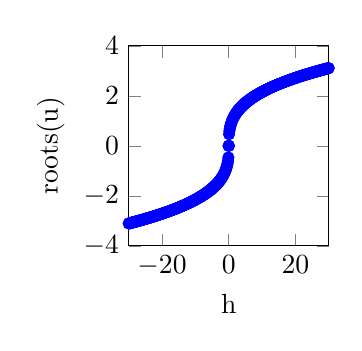
\begin{tikzpicture}

\begin{axis}[%
width=1in,
height=1in,
at={(0.758333in,0.48125in)},
scale only axis,
xmin=-30,
xmax=30,
xlabel={h},
ymin=-4,
ymax=4,
ylabel={roots(u)}
]
\addplot [color=blue,only marks,mark=*,mark options={solid},forget plot]
  table[row sep=crcr]{%
-30	-3.10723250595386\\
};
\addplot [color=blue,only marks,mark=*,mark options={solid},forget plot]
  table[row sep=crcr]{%
-29.9	-3.10377618218249\\
};
\addplot [color=blue,only marks,mark=*,mark options={solid},forget plot]
  table[row sep=crcr]{%
-29.8	-3.10031214338668\\
};
\addplot [color=blue,only marks,mark=*,mark options={solid},forget plot]
  table[row sep=crcr]{%
-29.7	-3.09684034636911\\
};
\addplot [color=blue,only marks,mark=*,mark options={solid},forget plot]
  table[row sep=crcr]{%
-29.6	-3.09336074754409\\
};
\addplot [color=blue,only marks,mark=*,mark options={solid},forget plot]
  table[row sep=crcr]{%
-29.5	-3.08987330293282\\
};
\addplot [color=blue,only marks,mark=*,mark options={solid},forget plot]
  table[row sep=crcr]{%
-29.4	-3.08637796815859\\
};
\addplot [color=blue,only marks,mark=*,mark options={solid},forget plot]
  table[row sep=crcr]{%
-29.3	-3.08287469844162\\
};
\addplot [color=blue,only marks,mark=*,mark options={solid},forget plot]
  table[row sep=crcr]{%
-29.2	-3.07936344859418\\
};
\addplot [color=blue,only marks,mark=*,mark options={solid},forget plot]
  table[row sep=crcr]{%
-29.1	-3.07584417301534\\
};
\addplot [color=blue,only marks,mark=*,mark options={solid},forget plot]
  table[row sep=crcr]{%
-29	-3.07231682568585\\
};
\addplot [color=blue,only marks,mark=*,mark options={solid},forget plot]
  table[row sep=crcr]{%
-28.9	-3.06878136016279\\
};
\addplot [color=blue,only marks,mark=*,mark options={solid},forget plot]
  table[row sep=crcr]{%
-28.8	-3.06523772957421\\
};
\addplot [color=blue,only marks,mark=*,mark options={solid},forget plot]
  table[row sep=crcr]{%
-28.7	-3.06168588661365\\
};
\addplot [color=blue,only marks,mark=*,mark options={solid},forget plot]
  table[row sep=crcr]{%
-28.6	-3.05812578353459\\
};
\addplot [color=blue,only marks,mark=*,mark options={solid},forget plot]
  table[row sep=crcr]{%
-28.5	-3.05455737214481\\
};
\addplot [color=blue,only marks,mark=*,mark options={solid},forget plot]
  table[row sep=crcr]{%
-28.4	-3.0509806038006\\
};
\addplot [color=blue,only marks,mark=*,mark options={solid},forget plot]
  table[row sep=crcr]{%
-28.3	-3.04739542940101\\
};
\addplot [color=blue,only marks,mark=*,mark options={solid},forget plot]
  table[row sep=crcr]{%
-28.2	-3.04380179938184\\
};
\addplot [color=blue,only marks,mark=*,mark options={solid},forget plot]
  table[row sep=crcr]{%
-28.1	-3.04019966370966\\
};
\addplot [color=blue,only marks,mark=*,mark options={solid},forget plot]
  table[row sep=crcr]{%
-28	-3.03658897187566\\
};
\addplot [color=blue,only marks,mark=*,mark options={solid},forget plot]
  table[row sep=crcr]{%
-27.9	-3.0329696728894\\
};
\addplot [color=blue,only marks,mark=*,mark options={solid},forget plot]
  table[row sep=crcr]{%
-27.8	-3.0293417152725\\
};
\addplot [color=blue,only marks,mark=*,mark options={solid},forget plot]
  table[row sep=crcr]{%
-27.7	-3.02570504705218\\
};
\addplot [color=blue,only marks,mark=*,mark options={solid},forget plot]
  table[row sep=crcr]{%
-27.6	-3.02205961575474\\
};
\addplot [color=blue,only marks,mark=*,mark options={solid},forget plot]
  table[row sep=crcr]{%
-27.5	-3.01840536839884\\
};
\addplot [color=blue,only marks,mark=*,mark options={solid},forget plot]
  table[row sep=crcr]{%
-27.4	-3.01474225148879\\
};
\addplot [color=blue,only marks,mark=*,mark options={solid},forget plot]
  table[row sep=crcr]{%
-27.3	-3.01107021100758\\
};
\addplot [color=blue,only marks,mark=*,mark options={solid},forget plot]
  table[row sep=crcr]{%
-27.2	-3.00738919240995\\
};
\addplot [color=blue,only marks,mark=*,mark options={solid},forget plot]
  table[row sep=crcr]{%
-27.1	-3.00369914061521\\
};
\addplot [color=blue,only marks,mark=*,mark options={solid},forget plot]
  table[row sep=crcr]{%
-27	-3\\
};
\addplot [color=blue,only marks,mark=*,mark options={solid},forget plot]
  table[row sep=crcr]{%
-26.9	-2.99629171439092\\
};
\addplot [color=blue,only marks,mark=*,mark options={solid},forget plot]
  table[row sep=crcr]{%
-26.8	-2.99257422705699\\
};
\addplot [color=blue,only marks,mark=*,mark options={solid},forget plot]
  table[row sep=crcr]{%
-26.7	-2.98884748070205\\
};
\addplot [color=blue,only marks,mark=*,mark options={solid},forget plot]
  table[row sep=crcr]{%
-26.6	-2.98511141745701\\
};
\addplot [color=blue,only marks,mark=*,mark options={solid},forget plot]
  table[row sep=crcr]{%
-26.5	-2.98136597887185\\
};
\addplot [color=blue,only marks,mark=*,mark options={solid},forget plot]
  table[row sep=crcr]{%
-26.4	-2.97761110590766\\
};
\addplot [color=blue,only marks,mark=*,mark options={solid},forget plot]
  table[row sep=crcr]{%
-26.3	-2.97384673892841\\
};
\addplot [color=blue,only marks,mark=*,mark options={solid},forget plot]
  table[row sep=crcr]{%
-26.2	-2.97007281769265\\
};
\addplot [color=blue,only marks,mark=*,mark options={solid},forget plot]
  table[row sep=crcr]{%
-26.1	-2.96628928134495\\
};
\addplot [color=blue,only marks,mark=*,mark options={solid},forget plot]
  table[row sep=crcr]{%
-26	-2.96249606840737\\
};
\addplot [color=blue,only marks,mark=*,mark options={solid},forget plot]
  table[row sep=crcr]{%
-25.9	-2.95869311677057\\
};
\addplot [color=blue,only marks,mark=*,mark options={solid},forget plot]
  table[row sep=crcr]{%
-25.8	-2.95488036368496\\
};
\addplot [color=blue,only marks,mark=*,mark options={solid},forget plot]
  table[row sep=crcr]{%
-25.7	-2.95105774575144\\
};
\addplot [color=blue,only marks,mark=*,mark options={solid},forget plot]
  table[row sep=crcr]{%
-25.6	-2.94722519891231\\
};
\addplot [color=blue,only marks,mark=*,mark options={solid},forget plot]
  table[row sep=crcr]{%
-25.5	-2.94338265844167\\
};
\addplot [color=blue,only marks,mark=*,mark options={solid},forget plot]
  table[row sep=crcr]{%
-25.4	-2.93953005893588\\
};
\addplot [color=blue,only marks,mark=*,mark options={solid},forget plot]
  table[row sep=crcr]{%
-25.3	-2.93566733430372\\
};
\addplot [color=blue,only marks,mark=*,mark options={solid},forget plot]
  table[row sep=crcr]{%
-25.2	-2.93179441775648\\
};
\addplot [color=blue,only marks,mark=*,mark options={solid},forget plot]
  table[row sep=crcr]{%
-25.1	-2.92791124179769\\
};
\addplot [color=blue,only marks,mark=*,mark options={solid},forget plot]
  table[row sep=crcr]{%
-25	-2.92401773821287\\
};
\addplot [color=blue,only marks,mark=*,mark options={solid},forget plot]
  table[row sep=crcr]{%
-24.9	-2.92011383805892\\
};
\addplot [color=blue,only marks,mark=*,mark options={solid},forget plot]
  table[row sep=crcr]{%
-24.8	-2.91619947165343\\
};
\addplot [color=blue,only marks,mark=*,mark options={solid},forget plot]
  table[row sep=crcr]{%
-24.7	-2.91227456856365\\
};
\addplot [color=blue,only marks,mark=*,mark options={solid},forget plot]
  table[row sep=crcr]{%
-24.6	-2.90833905759545\\
};
\addplot [color=blue,only marks,mark=*,mark options={solid},forget plot]
  table[row sep=crcr]{%
-24.5	-2.90439286678185\\
};
\addplot [color=blue,only marks,mark=*,mark options={solid},forget plot]
  table[row sep=crcr]{%
-24.4	-2.90043592337151\\
};
\addplot [color=blue,only marks,mark=*,mark options={solid},forget plot]
  table[row sep=crcr]{%
-24.3	-2.89646815381689\\
};
\addplot [color=blue,only marks,mark=*,mark options={solid},forget plot]
  table[row sep=crcr]{%
-24.2	-2.89248948376223\\
};
\addplot [color=blue,only marks,mark=*,mark options={solid},forget plot]
  table[row sep=crcr]{%
-24.1	-2.88849983803128\\
};
\addplot [color=blue,only marks,mark=*,mark options={solid},forget plot]
  table[row sep=crcr]{%
-24	-2.88449914061482\\
};
\addplot [color=blue,only marks,mark=*,mark options={solid},forget plot]
  table[row sep=crcr]{%
-23.9	-2.88048731465789\\
};
\addplot [color=blue,only marks,mark=*,mark options={solid},forget plot]
  table[row sep=crcr]{%
-23.8	-2.87646428244683\\
};
\addplot [color=blue,only marks,mark=*,mark options={solid},forget plot]
  table[row sep=crcr]{%
-23.7	-2.872429965396\\
};
\addplot [color=blue,only marks,mark=*,mark options={solid},forget plot]
  table[row sep=crcr]{%
-23.6	-2.86838428403424\\
};
\addplot [color=blue,only marks,mark=*,mark options={solid},forget plot]
  table[row sep=crcr]{%
-23.5	-2.86432715799122\\
};
\addplot [color=blue,only marks,mark=*,mark options={solid},forget plot]
  table[row sep=crcr]{%
-23.4	-2.86025850598323\\
};
\addplot [color=blue,only marks,mark=*,mark options={solid},forget plot]
  table[row sep=crcr]{%
-23.3	-2.85617824579896\\
};
\addplot [color=blue,only marks,mark=*,mark options={solid},forget plot]
  table[row sep=crcr]{%
-23.2	-2.85208629428482\\
};
\addplot [color=blue,only marks,mark=*,mark options={solid},forget plot]
  table[row sep=crcr]{%
-23.1	-2.84798256733006\\
};
\addplot [color=blue,only marks,mark=*,mark options={solid},forget plot]
  table[row sep=crcr]{%
-23	-2.84386697985156\\
};
\addplot [color=blue,only marks,mark=*,mark options={solid},forget plot]
  table[row sep=crcr]{%
-22.9	-2.83973944577827\\
};
\addplot [color=blue,only marks,mark=*,mark options={solid},forget plot]
  table[row sep=crcr]{%
-22.8	-2.83559987803539\\
};
\addplot [color=blue,only marks,mark=*,mark options={solid},forget plot]
  table[row sep=crcr]{%
-22.7	-2.83144818852819\\
};
\addplot [color=blue,only marks,mark=*,mark options={solid},forget plot]
  table[row sep=crcr]{%
-22.6	-2.82728428812555\\
};
\addplot [color=blue,only marks,mark=*,mark options={solid},forget plot]
  table[row sep=crcr]{%
-22.5	-2.82310808664309\\
};
\addplot [color=blue,only marks,mark=*,mark options={solid},forget plot]
  table[row sep=crcr]{%
-22.4	-2.81891949282596\\
};
\addplot [color=blue,only marks,mark=*,mark options={solid},forget plot]
  table[row sep=crcr]{%
-22.3	-2.81471841433133\\
};
\addplot [color=blue,only marks,mark=*,mark options={solid},forget plot]
  table[row sep=crcr]{%
-22.2	-2.81050475771048\\
};
\addplot [color=blue,only marks,mark=*,mark options={solid},forget plot]
  table[row sep=crcr]{%
-22.1	-2.80627842839044\\
};
\addplot [color=blue,only marks,mark=*,mark options={solid},forget plot]
  table[row sep=crcr]{%
-22	-2.80203933065539\\
};
\addplot [color=blue,only marks,mark=*,mark options={solid},forget plot]
  table[row sep=crcr]{%
-21.9	-2.79778736762753\\
};
\addplot [color=blue,only marks,mark=*,mark options={solid},forget plot]
  table[row sep=crcr]{%
-21.8	-2.79352244124763\\
};
\addplot [color=blue,only marks,mark=*,mark options={solid},forget plot]
  table[row sep=crcr]{%
-21.7	-2.7892444522551\\
};
\addplot [color=blue,only marks,mark=*,mark options={solid},forget plot]
  table[row sep=crcr]{%
-21.6	-2.78495330016767\\
};
\addplot [color=blue,only marks,mark=*,mark options={solid},forget plot]
  table[row sep=crcr]{%
-21.5	-2.78064888326061\\
};
\addplot [color=blue,only marks,mark=*,mark options={solid},forget plot]
  table[row sep=crcr]{%
-21.4	-2.77633109854556\\
};
\addplot [color=blue,only marks,mark=*,mark options={solid},forget plot]
  table[row sep=crcr]{%
-21.3	-2.77199984174875\\
};
\addplot [color=blue,only marks,mark=*,mark options={solid},forget plot]
  table[row sep=crcr]{%
-21.2	-2.76765500728892\\
};
\addplot [color=blue,only marks,mark=*,mark options={solid},forget plot]
  table[row sep=crcr]{%
-21.1	-2.76329648825463\\
};
\addplot [color=blue,only marks,mark=*,mark options={solid},forget plot]
  table[row sep=crcr]{%
-21	-2.75892417638112\\
};
\addplot [color=blue,only marks,mark=*,mark options={solid},forget plot]
  table[row sep=crcr]{%
-20.9	-2.75453796202665\\
};
\addplot [color=blue,only marks,mark=*,mark options={solid},forget plot]
  table[row sep=crcr]{%
-20.8	-2.75013773414828\\
};
\addplot [color=blue,only marks,mark=*,mark options={solid},forget plot]
  table[row sep=crcr]{%
-20.7	-2.74572338027716\\
};
\addplot [color=blue,only marks,mark=*,mark options={solid},forget plot]
  table[row sep=crcr]{%
-20.6	-2.7412947864932\\
};
\addplot [color=blue,only marks,mark=*,mark options={solid},forget plot]
  table[row sep=crcr]{%
-20.5	-2.73685183739921\\
};
\addplot [color=blue,only marks,mark=*,mark options={solid},forget plot]
  table[row sep=crcr]{%
-20.4	-2.73239441609447\\
};
\addplot [color=blue,only marks,mark=*,mark options={solid},forget plot]
  table[row sep=crcr]{%
-20.3	-2.72792240414759\\
};
\addplot [color=blue,only marks,mark=*,mark options={solid},forget plot]
  table[row sep=crcr]{%
-20.2	-2.72343568156888\\
};
\addplot [color=blue,only marks,mark=*,mark options={solid},forget plot]
  table[row sep=crcr]{%
-20.1	-2.71893412678198\\
};
\addplot [color=blue,only marks,mark=*,mark options={solid},forget plot]
  table[row sep=crcr]{%
-20	-2.71441761659491\\
};
\addplot [color=blue,only marks,mark=*,mark options={solid},forget plot]
  table[row sep=crcr]{%
-19.9	-2.70988602617033\\
};
\addplot [color=blue,only marks,mark=*,mark options={solid},forget plot]
  table[row sep=crcr]{%
-19.8	-2.70533922899524\\
};
\addplot [color=blue,only marks,mark=*,mark options={solid},forget plot]
  table[row sep=crcr]{%
-19.7	-2.70077709684987\\
};
\addplot [color=blue,only marks,mark=*,mark options={solid},forget plot]
  table[row sep=crcr]{%
-19.6	-2.69619949977585\\
};
\addplot [color=blue,only marks,mark=*,mark options={solid},forget plot]
  table[row sep=crcr]{%
-19.5	-2.69160630604364\\
};
\addplot [color=blue,only marks,mark=*,mark options={solid},forget plot]
  table[row sep=crcr]{%
-19.4	-2.68699738211917\\
};
\addplot [color=blue,only marks,mark=*,mark options={solid},forget plot]
  table[row sep=crcr]{%
-19.3	-2.68237259262967\\
};
\addplot [color=blue,only marks,mark=*,mark options={solid},forget plot]
  table[row sep=crcr]{%
-19.2	-2.67773180032868\\
};
\addplot [color=blue,only marks,mark=*,mark options={solid},forget plot]
  table[row sep=crcr]{%
-19.1	-2.6730748660602\\
};
\addplot [color=blue,only marks,mark=*,mark options={solid},forget plot]
  table[row sep=crcr]{%
-19	-2.66840164872194\\
};
\addplot [color=blue,only marks,mark=*,mark options={solid},forget plot]
  table[row sep=crcr]{%
-18.9	-2.6637120052278\\
};
\addplot [color=blue,only marks,mark=*,mark options={solid},forget plot]
  table[row sep=crcr]{%
-18.8	-2.65900579046917\\
};
\addplot [color=blue,only marks,mark=*,mark options={solid},forget plot]
  table[row sep=crcr]{%
-18.7	-2.65428285727552\\
};
\addplot [color=blue,only marks,mark=*,mark options={solid},forget plot]
  table[row sep=crcr]{%
-18.6	-2.64954305637382\\
};
\addplot [color=blue,only marks,mark=*,mark options={solid},forget plot]
  table[row sep=crcr]{%
-18.5	-2.6447862363471\\
};
\addplot [color=blue,only marks,mark=*,mark options={solid},forget plot]
  table[row sep=crcr]{%
-18.4	-2.64001224359183\\
};
\addplot [color=blue,only marks,mark=*,mark options={solid},forget plot]
  table[row sep=crcr]{%
-18.3	-2.63522092227424\\
};
\addplot [color=blue,only marks,mark=*,mark options={solid},forget plot]
  table[row sep=crcr]{%
-18.2	-2.63041211428563\\
};
\addplot [color=blue,only marks,mark=*,mark options={solid},forget plot]
  table[row sep=crcr]{%
-18.1	-2.62558565919638\\
};
\addplot [color=blue,only marks,mark=*,mark options={solid},forget plot]
  table[row sep=crcr]{%
-18	-2.6207413942089\\
};
\addplot [color=blue,only marks,mark=*,mark options={solid},forget plot]
  table[row sep=crcr]{%
-17.9	-2.61587915410925\\
};
\addplot [color=blue,only marks,mark=*,mark options={solid},forget plot]
  table[row sep=crcr]{%
-17.8	-2.61099877121762\\
};
\addplot [color=blue,only marks,mark=*,mark options={solid},forget plot]
  table[row sep=crcr]{%
-17.7	-2.60610007533735\\
};
\addplot [color=blue,only marks,mark=*,mark options={solid},forget plot]
  table[row sep=crcr]{%
-17.6	-2.60118289370278\\
};
\addplot [color=blue,only marks,mark=*,mark options={solid},forget plot]
  table[row sep=crcr]{%
-17.5	-2.59624705092555\\
};
\addplot [color=blue,only marks,mark=*,mark options={solid},forget plot]
  table[row sep=crcr]{%
-17.4	-2.59129236893962\\
};
\addplot [color=blue,only marks,mark=*,mark options={solid},forget plot]
  table[row sep=crcr]{%
-17.3	-2.58631866694467\\
};
\addplot [color=blue,only marks,mark=*,mark options={solid},forget plot]
  table[row sep=crcr]{%
-17.2	-2.58132576134807\\
};
\addplot [color=blue,only marks,mark=*,mark options={solid},forget plot]
  table[row sep=crcr]{%
-17.1	-2.5763134657052\\
};
\addplot [color=blue,only marks,mark=*,mark options={solid},forget plot]
  table[row sep=crcr]{%
-17	-2.57128159065823\\
};
\addplot [color=blue,only marks,mark=*,mark options={solid},forget plot]
  table[row sep=crcr]{%
-16.9	-2.56622994387314\\
};
\addplot [color=blue,only marks,mark=*,mark options={solid},forget plot]
  table[row sep=crcr]{%
-16.8	-2.56115832997499\\
};
\addplot [color=blue,only marks,mark=*,mark options={solid},forget plot]
  table[row sep=crcr]{%
-16.7	-2.55606655048144\\
};
\addplot [color=blue,only marks,mark=*,mark options={solid},forget plot]
  table[row sep=crcr]{%
-16.6	-2.55095440373441\\
};
\addplot [color=blue,only marks,mark=*,mark options={solid},forget plot]
  table[row sep=crcr]{%
-16.5	-2.54582168482974\\
};
\addplot [color=blue,only marks,mark=*,mark options={solid},forget plot]
  table[row sep=crcr]{%
-16.4	-2.54066818554496\\
};
\addplot [color=blue,only marks,mark=*,mark options={solid},forget plot]
  table[row sep=crcr]{%
-16.3	-2.5354936942649\\
};
\addplot [color=blue,only marks,mark=*,mark options={solid},forget plot]
  table[row sep=crcr]{%
-16.2	-2.53029799590525\\
};
\addplot [color=blue,only marks,mark=*,mark options={solid},forget plot]
  table[row sep=crcr]{%
-16.1	-2.52508087183385\\
};
\addplot [color=blue,only marks,mark=*,mark options={solid},forget plot]
  table[row sep=crcr]{%
-16	-2.51984209978975\\
};
\addplot [color=blue,only marks,mark=*,mark options={solid},forget plot]
  table[row sep=crcr]{%
-15.9	-2.51458145379984\\
};
\addplot [color=blue,only marks,mark=*,mark options={solid},forget plot]
  table[row sep=crcr]{%
-15.8	-2.5092987040931\\
};
\addplot [color=blue,only marks,mark=*,mark options={solid},forget plot]
  table[row sep=crcr]{%
-15.7	-2.50399361701225\\
};
\addplot [color=blue,only marks,mark=*,mark options={solid},forget plot]
  table[row sep=crcr]{%
-15.6	-2.49866595492278\\
};
\addplot [color=blue,only marks,mark=*,mark options={solid},forget plot]
  table[row sep=crcr]{%
-15.5	-2.49331547611933\\
};
\addplot [color=blue,only marks,mark=*,mark options={solid},forget plot]
  table[row sep=crcr]{%
-15.4	-2.48794193472908\\
};
\addplot [color=blue,only marks,mark=*,mark options={solid},forget plot]
  table[row sep=crcr]{%
-15.3	-2.4825450806124\\
};
\addplot [color=blue,only marks,mark=*,mark options={solid},forget plot]
  table[row sep=crcr]{%
-15.2	-2.47712465926034\\
};
\addplot [color=blue,only marks,mark=*,mark options={solid},forget plot]
  table[row sep=crcr]{%
-15.1	-2.47168041168896\\
};
\addplot [color=blue,only marks,mark=*,mark options={solid},forget plot]
  table[row sep=crcr]{%
-15	-2.46621207433047\\
};
\addplot [color=blue,only marks,mark=*,mark options={solid},forget plot]
  table[row sep=crcr]{%
-14.9	-2.4607193789209\\
};
\addplot [color=blue,only marks,mark=*,mark options={solid},forget plot]
  table[row sep=crcr]{%
-14.8	-2.45520205238429\\
};
\addplot [color=blue,only marks,mark=*,mark options={solid},forget plot]
  table[row sep=crcr]{%
-14.7	-2.44965981671321\\
};
\addplot [color=blue,only marks,mark=*,mark options={solid},forget plot]
  table[row sep=crcr]{%
-14.6	-2.44409238884541\\
};
\addplot [color=blue,only marks,mark=*,mark options={solid},forget plot]
  table[row sep=crcr]{%
-14.5	-2.43849948053666\\
};
\addplot [color=blue,only marks,mark=*,mark options={solid},forget plot]
  table[row sep=crcr]{%
-14.4	-2.43288079822936\\
};
\addplot [color=blue,only marks,mark=*,mark options={solid},forget plot]
  table[row sep=crcr]{%
-14.3	-2.42723604291695\\
};
\addplot [color=blue,only marks,mark=*,mark options={solid},forget plot]
  table[row sep=crcr]{%
-14.2	-2.42156491000382\\
};
\addplot [color=blue,only marks,mark=*,mark options={solid},forget plot]
  table[row sep=crcr]{%
-14.1	-2.41586708916072\\
};
\addplot [color=blue,only marks,mark=*,mark options={solid},forget plot]
  table[row sep=crcr]{%
-14	-2.41014226417523\\
};
\addplot [color=blue,only marks,mark=*,mark options={solid},forget plot]
  table[row sep=crcr]{%
-13.9	-2.40439011279735\\
};
\addplot [color=blue,only marks,mark=*,mark options={solid},forget plot]
  table[row sep=crcr]{%
-13.8	-2.39861030657984\\
};
\addplot [color=blue,only marks,mark=*,mark options={solid},forget plot]
  table[row sep=crcr]{%
-13.7	-2.39280251071314\\
};
\addplot [color=blue,only marks,mark=*,mark options={solid},forget plot]
  table[row sep=crcr]{%
-13.6	-2.38696638385467\\
};
\addplot [color=blue,only marks,mark=*,mark options={solid},forget plot]
  table[row sep=crcr]{%
-13.5	-2.3811015779523\\
};
\addplot [color=blue,only marks,mark=*,mark options={solid},forget plot]
  table[row sep=crcr]{%
-13.4	-2.37520773806159\\
};
\addplot [color=blue,only marks,mark=*,mark options={solid},forget plot]
  table[row sep=crcr]{%
-13.3	-2.36928450215677\\
};
\addplot [color=blue,only marks,mark=*,mark options={solid},forget plot]
  table[row sep=crcr]{%
-13.2	-2.363331500935\\
};
\addplot [color=blue,only marks,mark=*,mark options={solid},forget plot]
  table[row sep=crcr]{%
-13.1	-2.35734835761373\\
};
\addplot [color=blue,only marks,mark=*,mark options={solid},forget plot]
  table[row sep=crcr]{%
-13	-2.35133468772076\\
};
\addplot [color=blue,only marks,mark=*,mark options={solid},forget plot]
  table[row sep=crcr]{%
-12.9	-2.34529009887684\\
};
\addplot [color=blue,only marks,mark=*,mark options={solid},forget plot]
  table[row sep=crcr]{%
-12.8	-2.33921419057029\\
};
\addplot [color=blue,only marks,mark=*,mark options={solid},forget plot]
  table[row sep=crcr]{%
-12.7	-2.33310655392348\\
};
\addplot [color=blue,only marks,mark=*,mark options={solid},forget plot]
  table[row sep=crcr]{%
-12.6	-2.32696677145056\\
};
\addplot [color=blue,only marks,mark=*,mark options={solid},forget plot]
  table[row sep=crcr]{%
-12.5	-2.32079441680639\\
};
\addplot [color=blue,only marks,mark=*,mark options={solid},forget plot]
  table[row sep=crcr]{%
-12.4	-2.31458905452587\\
};
\addplot [color=blue,only marks,mark=*,mark options={solid},forget plot]
  table[row sep=crcr]{%
-12.3	-2.30835023975361\\
};
\addplot [color=blue,only marks,mark=*,mark options={solid},forget plot]
  table[row sep=crcr]{%
-12.2	-2.30207751796315\\
};
\addplot [color=blue,only marks,mark=*,mark options={solid},forget plot]
  table[row sep=crcr]{%
-12.1	-2.29577042466555\\
};
\addplot [color=blue,only marks,mark=*,mark options={solid},forget plot]
  table[row sep=crcr]{%
-12	-2.28942848510666\\
};
\addplot [color=blue,only marks,mark=*,mark options={solid},forget plot]
  table[row sep=crcr]{%
-11.9	-2.28305121395253\\
};
\addplot [color=blue,only marks,mark=*,mark options={solid},forget plot]
  table[row sep=crcr]{%
-11.8	-2.2766381149625\\
};
\addplot [color=blue,only marks,mark=*,mark options={solid},forget plot]
  table[row sep=crcr]{%
-11.7	-2.27018868064939\\
};
\addplot [color=blue,only marks,mark=*,mark options={solid},forget plot]
  table[row sep=crcr]{%
-11.6	-2.2637023919259\\
};
\addplot [color=blue,only marks,mark=*,mark options={solid},forget plot]
  table[row sep=crcr]{%
-11.5	-2.257178717737\\
};
\addplot [color=blue,only marks,mark=*,mark options={solid},forget plot]
  table[row sep=crcr]{%
-11.4	-2.25061711467713\\
};
\addplot [color=blue,only marks,mark=*,mark options={solid},forget plot]
  table[row sep=crcr]{%
-11.3	-2.24401702659183\\
};
\addplot [color=blue,only marks,mark=*,mark options={solid},forget plot]
  table[row sep=crcr]{%
-11.2	-2.2373778841628\\
};
\addplot [color=blue,only marks,mark=*,mark options={solid},forget plot]
  table[row sep=crcr]{%
-11.1	-2.23069910447562\\
};
\addplot [color=blue,only marks,mark=*,mark options={solid},forget plot]
  table[row sep=crcr]{%
-11	-2.22398009056931\\
};
\addplot [color=blue,only marks,mark=*,mark options={solid},forget plot]
  table[row sep=crcr]{%
-10.9	-2.21722023096663\\
};
\addplot [color=blue,only marks,mark=*,mark options={solid},forget plot]
  table[row sep=crcr]{%
-10.8	-2.21041889918423\\
};
\addplot [color=blue,only marks,mark=*,mark options={solid},forget plot]
  table[row sep=crcr]{%
-10.7	-2.20357545322163\\
};
\addplot [color=blue,only marks,mark=*,mark options={solid},forget plot]
  table[row sep=crcr]{%
-10.6	-2.19668923502774\\
};
\addplot [color=blue,only marks,mark=*,mark options={solid},forget plot]
  table[row sep=crcr]{%
-10.5	-2.18975956994394\\
};
\addplot [color=blue,only marks,mark=*,mark options={solid},forget plot]
  table[row sep=crcr]{%
-10.4	-2.18278576612221\\
};
\addplot [color=blue,only marks,mark=*,mark options={solid},forget plot]
  table[row sep=crcr]{%
-10.3	-2.17576711391712\\
};
\addplot [color=blue,only marks,mark=*,mark options={solid},forget plot]
  table[row sep=crcr]{%
-10.2	-2.1687028852502\\
};
\addplot [color=blue,only marks,mark=*,mark options={solid},forget plot]
  table[row sep=crcr]{%
-10.1	-2.16159233294508\\
};
\addplot [color=blue,only marks,mark=*,mark options={solid},forget plot]
  table[row sep=crcr]{%
-10	-2.15443469003188\\
};
\addplot [color=blue,only marks,mark=*,mark options={solid},forget plot]
  table[row sep=crcr]{%
-9.9	-2.14722916901894\\
};
\addplot [color=blue,only marks,mark=*,mark options={solid},forget plot]
  table[row sep=crcr]{%
-9.8	-2.13997496113016\\
};
\addplot [color=blue,only marks,mark=*,mark options={solid},forget plot]
  table[row sep=crcr]{%
-9.7	-2.13267123550589\\
};
\addplot [color=blue,only marks,mark=*,mark options={solid},forget plot]
  table[row sep=crcr]{%
-9.6	-2.12531713836522\\
};
\addplot [color=blue,only marks,mark=*,mark options={solid},forget plot]
  table[row sep=crcr]{%
-9.5	-2.11791179212745\\
};
\addplot [color=blue,only marks,mark=*,mark options={solid},forget plot]
  table[row sep=crcr]{%
-9.4	-2.11045429449015\\
};
\addplot [color=blue,only marks,mark=*,mark options={solid},forget plot]
  table[row sep=crcr]{%
-9.3	-2.10294371746142\\
};
\addplot [color=blue,only marks,mark=*,mark options={solid},forget plot]
  table[row sep=crcr]{%
-9.2	-2.09537910634329\\
};
\addplot [color=blue,only marks,mark=*,mark options={solid},forget plot]
  table[row sep=crcr]{%
-9.1	-2.08775947866345\\
};
\addplot [color=blue,only marks,mark=*,mark options={solid},forget plot]
  table[row sep=crcr]{%
-9	-2.08008382305191\\
};
\addplot [color=blue,only marks,mark=*,mark options={solid},forget plot]
  table[row sep=crcr]{%
-8.9	-2.07235109805926\\
};
\addplot [color=blue,only marks,mark=*,mark options={solid},forget plot]
  table[row sep=crcr]{%
-8.8	-2.06456023091273\\
};
\addplot [color=blue,only marks,mark=*,mark options={solid},forget plot]
  table[row sep=crcr]{%
-8.7	-2.05671011620596\\
};
\addplot [color=blue,only marks,mark=*,mark options={solid},forget plot]
  table[row sep=crcr]{%
-8.6	-2.04879961451827\\
};
\addplot [color=blue,only marks,mark=*,mark options={solid},forget plot]
  table[row sep=crcr]{%
-8.5	-2.04082755095868\\
};
\addplot [color=blue,only marks,mark=*,mark options={solid},forget plot]
  table[row sep=crcr]{%
-8.4	-2.03279271362971\\
};
\addplot [color=blue,only marks,mark=*,mark options={solid},forget plot]
  table[row sep=crcr]{%
-8.3	-2.02469385200545\\
};
\addplot [color=blue,only marks,mark=*,mark options={solid},forget plot]
  table[row sep=crcr]{%
-8.2	-2.0165296752181\\
};
\addplot [color=blue,only marks,mark=*,mark options={solid},forget plot]
  table[row sep=crcr]{%
-8.1	-2.00829885024651\\
};
\addplot [color=blue,only marks,mark=*,mark options={solid},forget plot]
  table[row sep=crcr]{%
-8	-2\\
};
\addplot [color=blue,only marks,mark=*,mark options={solid},forget plot]
  table[row sep=crcr]{%
-7.9	-1.99163170128991\\
};
\addplot [color=blue,only marks,mark=*,mark options={solid},forget plot]
  table[row sep=crcr]{%
-7.8	-1.98319248268077\\
};
\addplot [color=blue,only marks,mark=*,mark options={solid},forget plot]
  table[row sep=crcr]{%
-7.7	-1.97468082221237\\
};
\addplot [color=blue,only marks,mark=*,mark options={solid},forget plot]
  table[row sep=crcr]{%
-7.6	-1.96609514498312\\
};
\addplot [color=blue,only marks,mark=*,mark options={solid},forget plot]
  table[row sep=crcr]{%
-7.5	-1.95743382058443\\
};
\addplot [color=blue,only marks,mark=*,mark options={solid},forget plot]
  table[row sep=crcr]{%
-7.4	-1.94869516037466\\
};
\addplot [color=blue,only marks,mark=*,mark options={solid},forget plot]
  table[row sep=crcr]{%
-7.3	-1.93987741458033\\
};
\addplot [color=blue,only marks,mark=*,mark options={solid},forget plot]
  table[row sep=crcr]{%
-7.2	-1.93097876921126\\
};
\addplot [color=blue,only marks,mark=*,mark options={solid},forget plot]
  table[row sep=crcr]{%
-7.1	-1.92199734277467\\
};
\addplot [color=blue,only marks,mark=*,mark options={solid},forget plot]
  table[row sep=crcr]{%
-7	-1.91293118277239\\
};
\addplot [color=blue,only marks,mark=*,mark options={solid},forget plot]
  table[row sep=crcr]{%
-6.9	-1.9037782619633\\
};
\addplot [color=blue,only marks,mark=*,mark options={solid},forget plot]
  table[row sep=crcr]{%
-6.8	-1.89453647437182\\
};
\addplot [color=blue,only marks,mark=*,mark options={solid},forget plot]
  table[row sep=crcr]{%
-6.7	-1.88520363102098\\
};
\addplot [color=blue,only marks,mark=*,mark options={solid},forget plot]
  table[row sep=crcr]{%
-6.6	-1.8757774553669\\
};
\addplot [color=blue,only marks,mark=*,mark options={solid},forget plot]
  table[row sep=crcr]{%
-6.5	-1.86625557840862\\
};
\addplot [color=blue,only marks,mark=*,mark options={solid},forget plot]
  table[row sep=crcr]{%
-6.4	-1.85663553344511\\
};
\addplot [color=blue,only marks,mark=*,mark options={solid},forget plot]
  table[row sep=crcr]{%
-6.3	-1.84691475044783\\
};
\addplot [color=blue,only marks,mark=*,mark options={solid},forget plot]
  table[row sep=crcr]{%
-6.2	-1.83709055001423\\
};
\addplot [color=blue,only marks,mark=*,mark options={solid},forget plot]
  table[row sep=crcr]{%
-6.1	-1.82716013686352\\
};
\addplot [color=blue,only marks,mark=*,mark options={solid},forget plot]
  table[row sep=crcr]{%
-6	-1.81712059283214\\
};
\addplot [color=blue,only marks,mark=*,mark options={solid},forget plot]
  table[row sep=crcr]{%
-5.9	-1.80696886932119\\
};
\addplot [color=blue,only marks,mark=*,mark options={solid},forget plot]
  table[row sep=crcr]{%
-5.8	-1.79670177914305\\
};
\addplot [color=blue,only marks,mark=*,mark options={solid},forget plot]
  table[row sep=crcr]{%
-5.7	-1.78631598770806\\
};
\addplot [color=blue,only marks,mark=*,mark options={solid},forget plot]
  table[row sep=crcr]{%
-5.6	-1.7758080034852\\
};
\addplot [color=blue,only marks,mark=*,mark options={solid},forget plot]
  table[row sep=crcr]{%
-5.5	-1.76517416766303\\
};
\addplot [color=blue,only marks,mark=*,mark options={solid},forget plot]
  table[row sep=crcr]{%
-5.4	-1.75441064292772\\
};
\addplot [color=blue,only marks,mark=*,mark options={solid},forget plot]
  table[row sep=crcr]{%
-5.3	-1.74351340126513\\
};
\addplot [color=blue,only marks,mark=*,mark options={solid},forget plot]
  table[row sep=crcr]{%
-5.2	-1.73247821068181\\
};
\addplot [color=blue,only marks,mark=*,mark options={solid},forget plot]
  table[row sep=crcr]{%
-5.1	-1.72130062072632\\
};
\addplot [color=blue,only marks,mark=*,mark options={solid},forget plot]
  table[row sep=crcr]{%
-5	-1.7099759466767\\
};
\addplot [color=blue,only marks,mark=*,mark options={solid},forget plot]
  table[row sep=crcr]{%
-4.9	-1.69849925224181\\
};
\addplot [color=blue,only marks,mark=*,mark options={solid},forget plot]
  table[row sep=crcr]{%
-4.8	-1.6868653306035\\
};
\addplot [color=blue,only marks,mark=*,mark options={solid},forget plot]
  table[row sep=crcr]{%
-4.7	-1.67506868360223\\
};
\addplot [color=blue,only marks,mark=*,mark options={solid},forget plot]
  table[row sep=crcr]{%
-4.6	-1.66310349884077\\
};
\addplot [color=blue,only marks,mark=*,mark options={solid},forget plot]
  table[row sep=crcr]{%
-4.5	-1.65096362444731\\
};
\addplot [color=blue,only marks,mark=*,mark options={solid},forget plot]
  table[row sep=crcr]{%
-4.4	-1.63864254120129\\
};
\addplot [color=blue,only marks,mark=*,mark options={solid},forget plot]
  table[row sep=crcr]{%
-4.3	-1.62613333167917\\
};
\addplot [color=blue,only marks,mark=*,mark options={solid},forget plot]
  table[row sep=crcr]{%
-4.2	-1.61342864602455\\
};
\addplot [color=blue,only marks,mark=*,mark options={solid},forget plot]
  table[row sep=crcr]{%
-4.1	-1.60052066388315\\
};
\addplot [color=blue,only marks,mark=*,mark options={solid},forget plot]
  table[row sep=crcr]{%
-4	-1.5874010519682\\
};
\addplot [color=blue,only marks,mark=*,mark options={solid},forget plot]
  table[row sep=crcr]{%
-3.9	-1.57406091663144\\
};
\addplot [color=blue,only marks,mark=*,mark options={solid},forget plot]
  table[row sep=crcr]{%
-3.8	-1.56049075070788\\
};
\addplot [color=blue,only marks,mark=*,mark options={solid},forget plot]
  table[row sep=crcr]{%
-3.7	-1.54668037377204\\
};
\addplot [color=blue,only marks,mark=*,mark options={solid},forget plot]
  table[row sep=crcr]{%
-3.6	-1.53261886478711\\
};
\addplot [color=blue,only marks,mark=*,mark options={solid},forget plot]
  table[row sep=crcr]{%
-3.5	-1.51829448593783\\
};
\addplot [color=blue,only marks,mark=*,mark options={solid},forget plot]
  table[row sep=crcr]{%
-3.4	-1.50369459620497\\
};
\addplot [color=blue,only marks,mark=*,mark options={solid},forget plot]
  table[row sep=crcr]{%
-3.3	-1.48880555295383\\
};
\addplot [color=blue,only marks,mark=*,mark options={solid},forget plot]
  table[row sep=crcr]{%
-3.2	-1.47361259945616\\
};
\addplot [color=blue,only marks,mark=*,mark options={solid},forget plot]
  table[row sep=crcr]{%
-3.1	-1.45809973582671\\
};
\addplot [color=blue,only marks,mark=*,mark options={solid},forget plot]
  table[row sep=crcr]{%
-3	-1.44224957030741\\
};
\addplot [color=blue,only marks,mark=*,mark options={solid},forget plot]
  table[row sep=crcr]{%
-2.9	-1.42604314714241\\
};
\addplot [color=blue,only marks,mark=*,mark options={solid},forget plot]
  table[row sep=crcr]{%
-2.8	-1.40945974641298\\
};
\addplot [color=blue,only marks,mark=*,mark options={solid},forget plot]
  table[row sep=crcr]{%
-2.7	-1.39247665008383\\
};
\addplot [color=blue,only marks,mark=*,mark options={solid},forget plot]
  table[row sep=crcr]{%
-2.6	-1.37506886707414\\
};
\addplot [color=blue,only marks,mark=*,mark options={solid},forget plot]
  table[row sep=crcr]{%
-2.5	-1.35720880829745\\
};
\addplot [color=blue,only marks,mark=*,mark options={solid},forget plot]
  table[row sep=crcr]{%
-2.4	-1.33886590016434\\
};
\addplot [color=blue,only marks,mark=*,mark options={solid},forget plot]
  table[row sep=crcr]{%
-2.3	-1.32000612179591\\
};
\addplot [color=blue,only marks,mark=*,mark options={solid},forget plot]
  table[row sep=crcr]{%
-2.2	-1.30059144685139\\
};
\addplot [color=blue,only marks,mark=*,mark options={solid},forget plot]
  table[row sep=crcr]{%
-2.1	-1.28057916498749\\
};
\addplot [color=blue,only marks,mark=*,mark options={solid},forget plot]
  table[row sep=crcr]{%
-2	-1.25992104989487\\
};
\addplot [color=blue,only marks,mark=*,mark options={solid},forget plot]
  table[row sep=crcr]{%
-1.9	-1.23856232963017\\
};
\addplot [color=blue,only marks,mark=*,mark options={solid},forget plot]
  table[row sep=crcr]{%
-1.8	-1.21644039911468\\
};
\addplot [color=blue,only marks,mark=*,mark options={solid},forget plot]
  table[row sep=crcr]{%
-1.7	-1.19348319192734\\
};
\addplot [color=blue,only marks,mark=*,mark options={solid},forget plot]
  table[row sep=crcr]{%
-1.6	-1.16960709528515\\
};
\addplot [color=blue,only marks,mark=*,mark options={solid},forget plot]
  table[row sep=crcr]{%
-1.5	-1.14471424255333\\
};
\addplot [color=blue,only marks,mark=*,mark options={solid},forget plot]
  table[row sep=crcr]{%
-1.4	-1.1186889420814\\
};
\addplot [color=blue,only marks,mark=*,mark options={solid},forget plot]
  table[row sep=crcr]{%
-1.3	-1.09139288306111\\
};
\addplot [color=blue,only marks,mark=*,mark options={solid},forget plot]
  table[row sep=crcr]{%
-1.2	-1.06265856918261\\
};
\addplot [color=blue,only marks,mark=*,mark options={solid},forget plot]
  table[row sep=crcr]{%
-1.1	-1.03228011545637\\
};
\addplot [color=blue,only marks,mark=*,mark options={solid},forget plot]
  table[row sep=crcr]{%
-1	-1\\
};
\addplot [color=blue,only marks,mark=*,mark options={solid},forget plot]
  table[row sep=crcr]{%
-0.899999999999999	-0.965489384605629\\
};
\addplot [color=blue,only marks,mark=*,mark options={solid},forget plot]
  table[row sep=crcr]{%
-0.799999999999997	-0.928317766722555\\
};
\addplot [color=blue,only marks,mark=*,mark options={solid},forget plot]
  table[row sep=crcr]{%
-0.699999999999999	-0.887904001742601\\
};
\addplot [color=blue,only marks,mark=*,mark options={solid},forget plot]
  table[row sep=crcr]{%
-0.599999999999998	-0.843432665301749\\
};
\addplot [color=blue,only marks,mark=*,mark options={solid},forget plot]
  table[row sep=crcr]{%
-0.5	-0.793700525984101\\
};
\addplot [color=blue,only marks,mark=*,mark options={solid},forget plot]
  table[row sep=crcr]{%
-0.399999999999999	-0.736806299728076\\
};
\addplot [color=blue,only marks,mark=*,mark options={solid},forget plot]
  table[row sep=crcr]{%
-0.299999999999997	-0.669432950082167\\
};
\addplot [color=blue,only marks,mark=*,mark options={solid},forget plot]
  table[row sep=crcr]{%
-0.199999999999999	-0.584803547642572\\
};
\addplot [color=blue,only marks,mark=*,mark options={solid},forget plot]
  table[row sep=crcr]{%
-0.0999999999999979	-0.464158883361275\\
};
\addplot [color=blue,only marks,mark=*,mark options={solid},forget plot]
  table[row sep=crcr]{%
0	0\\
};
\addplot [color=blue,only marks,mark=*,mark options={solid},forget plot]
  table[row sep=crcr]{%
0	0\\
};
\addplot [color=blue,only marks,mark=*,mark options={solid},forget plot]
  table[row sep=crcr]{%
0	0\\
};
\addplot [color=blue,only marks,mark=*,mark options={solid},forget plot]
  table[row sep=crcr]{%
0.100000000000001	0.46415888336128\\
};
\addplot [color=blue,only marks,mark=*,mark options={solid},forget plot]
  table[row sep=crcr]{%
0.200000000000003	0.584803547642576\\
};
\addplot [color=blue,only marks,mark=*,mark options={solid},forget plot]
  table[row sep=crcr]{%
0.300000000000001	0.66943295008217\\
};
\addplot [color=blue,only marks,mark=*,mark options={solid},forget plot]
  table[row sep=crcr]{%
0.400000000000002	0.736806299728079\\
};
\addplot [color=blue,only marks,mark=*,mark options={solid},forget plot]
  table[row sep=crcr]{%
0.5	0.7937005259841\\
};
\addplot [color=blue,only marks,mark=*,mark options={solid},forget plot]
  table[row sep=crcr]{%
0.600000000000001	0.84343266530175\\
};
\addplot [color=blue,only marks,mark=*,mark options={solid},forget plot]
  table[row sep=crcr]{%
0.700000000000003	0.887904001742602\\
};
\addplot [color=blue,only marks,mark=*,mark options={solid},forget plot]
  table[row sep=crcr]{%
0.800000000000001	0.928317766722556\\
};
\addplot [color=blue,only marks,mark=*,mark options={solid},forget plot]
  table[row sep=crcr]{%
0.900000000000002	0.96548938460563\\
};
\addplot [color=blue,only marks,mark=*,mark options={solid},forget plot]
  table[row sep=crcr]{%
1	1\\
};
\addplot [color=blue,only marks,mark=*,mark options={solid},forget plot]
  table[row sep=crcr]{%
1.1	1.03228011545637\\
};
\addplot [color=blue,only marks,mark=*,mark options={solid},forget plot]
  table[row sep=crcr]{%
1.2	1.06265856918261\\
};
\addplot [color=blue,only marks,mark=*,mark options={solid},forget plot]
  table[row sep=crcr]{%
1.3	1.09139288306111\\
};
\addplot [color=blue,only marks,mark=*,mark options={solid},forget plot]
  table[row sep=crcr]{%
1.4	1.1186889420814\\
};
\addplot [color=blue,only marks,mark=*,mark options={solid},forget plot]
  table[row sep=crcr]{%
1.5	1.14471424255333\\
};
\addplot [color=blue,only marks,mark=*,mark options={solid},forget plot]
  table[row sep=crcr]{%
1.6	1.16960709528515\\
};
\addplot [color=blue,only marks,mark=*,mark options={solid},forget plot]
  table[row sep=crcr]{%
1.7	1.19348319192734\\
};
\addplot [color=blue,only marks,mark=*,mark options={solid},forget plot]
  table[row sep=crcr]{%
1.8	1.21644039911468\\
};
\addplot [color=blue,only marks,mark=*,mark options={solid},forget plot]
  table[row sep=crcr]{%
1.9	1.23856232963017\\
};
\addplot [color=blue,only marks,mark=*,mark options={solid},forget plot]
  table[row sep=crcr]{%
2	1.25992104989487\\
};
\addplot [color=blue,only marks,mark=*,mark options={solid},forget plot]
  table[row sep=crcr]{%
2.1	1.28057916498749\\
};
\addplot [color=blue,only marks,mark=*,mark options={solid},forget plot]
  table[row sep=crcr]{%
2.2	1.30059144685139\\
};
\addplot [color=blue,only marks,mark=*,mark options={solid},forget plot]
  table[row sep=crcr]{%
2.3	1.32000612179591\\
};
\addplot [color=blue,only marks,mark=*,mark options={solid},forget plot]
  table[row sep=crcr]{%
2.4	1.33886590016434\\
};
\addplot [color=blue,only marks,mark=*,mark options={solid},forget plot]
  table[row sep=crcr]{%
2.5	1.35720880829745\\
};
\addplot [color=blue,only marks,mark=*,mark options={solid},forget plot]
  table[row sep=crcr]{%
2.6	1.37506886707414\\
};
\addplot [color=blue,only marks,mark=*,mark options={solid},forget plot]
  table[row sep=crcr]{%
2.7	1.39247665008383\\
};
\addplot [color=blue,only marks,mark=*,mark options={solid},forget plot]
  table[row sep=crcr]{%
2.8	1.40945974641298\\
};
\addplot [color=blue,only marks,mark=*,mark options={solid},forget plot]
  table[row sep=crcr]{%
2.9	1.42604314714241\\
};
\addplot [color=blue,only marks,mark=*,mark options={solid},forget plot]
  table[row sep=crcr]{%
3	1.44224957030741\\
};
\addplot [color=blue,only marks,mark=*,mark options={solid},forget plot]
  table[row sep=crcr]{%
3.1	1.45809973582671\\
};
\addplot [color=blue,only marks,mark=*,mark options={solid},forget plot]
  table[row sep=crcr]{%
3.2	1.47361259945615\\
};
\addplot [color=blue,only marks,mark=*,mark options={solid},forget plot]
  table[row sep=crcr]{%
3.3	1.48880555295383\\
};
\addplot [color=blue,only marks,mark=*,mark options={solid},forget plot]
  table[row sep=crcr]{%
3.4	1.50369459620497\\
};
\addplot [color=blue,only marks,mark=*,mark options={solid},forget plot]
  table[row sep=crcr]{%
3.5	1.51829448593783\\
};
\addplot [color=blue,only marks,mark=*,mark options={solid},forget plot]
  table[row sep=crcr]{%
3.6	1.53261886478711\\
};
\addplot [color=blue,only marks,mark=*,mark options={solid},forget plot]
  table[row sep=crcr]{%
3.7	1.54668037377204\\
};
\addplot [color=blue,only marks,mark=*,mark options={solid},forget plot]
  table[row sep=crcr]{%
3.8	1.56049075070789\\
};
\addplot [color=blue,only marks,mark=*,mark options={solid},forget plot]
  table[row sep=crcr]{%
3.9	1.57406091663144\\
};
\addplot [color=blue,only marks,mark=*,mark options={solid},forget plot]
  table[row sep=crcr]{%
4	1.5874010519682\\
};
\addplot [color=blue,only marks,mark=*,mark options={solid},forget plot]
  table[row sep=crcr]{%
4.1	1.60052066388316\\
};
\addplot [color=blue,only marks,mark=*,mark options={solid},forget plot]
  table[row sep=crcr]{%
4.2	1.61342864602454\\
};
\addplot [color=blue,only marks,mark=*,mark options={solid},forget plot]
  table[row sep=crcr]{%
4.3	1.62613333167917\\
};
\addplot [color=blue,only marks,mark=*,mark options={solid},forget plot]
  table[row sep=crcr]{%
4.4	1.63864254120129\\
};
\addplot [color=blue,only marks,mark=*,mark options={solid},forget plot]
  table[row sep=crcr]{%
4.5	1.65096362444731\\
};
\addplot [color=blue,only marks,mark=*,mark options={solid},forget plot]
  table[row sep=crcr]{%
4.6	1.66310349884077\\
};
\addplot [color=blue,only marks,mark=*,mark options={solid},forget plot]
  table[row sep=crcr]{%
4.7	1.67506868360224\\
};
\addplot [color=blue,only marks,mark=*,mark options={solid},forget plot]
  table[row sep=crcr]{%
4.8	1.6868653306035\\
};
\addplot [color=blue,only marks,mark=*,mark options={solid},forget plot]
  table[row sep=crcr]{%
4.9	1.69849925224181\\
};
\addplot [color=blue,only marks,mark=*,mark options={solid},forget plot]
  table[row sep=crcr]{%
5	1.7099759466767\\
};
\addplot [color=blue,only marks,mark=*,mark options={solid},forget plot]
  table[row sep=crcr]{%
5.1	1.72130062072632\\
};
\addplot [color=blue,only marks,mark=*,mark options={solid},forget plot]
  table[row sep=crcr]{%
5.2	1.73247821068181\\
};
\addplot [color=blue,only marks,mark=*,mark options={solid},forget plot]
  table[row sep=crcr]{%
5.3	1.74351340126513\\
};
\addplot [color=blue,only marks,mark=*,mark options={solid},forget plot]
  table[row sep=crcr]{%
5.4	1.75441064292772\\
};
\addplot [color=blue,only marks,mark=*,mark options={solid},forget plot]
  table[row sep=crcr]{%
5.5	1.76517416766303\\
};
\addplot [color=blue,only marks,mark=*,mark options={solid},forget plot]
  table[row sep=crcr]{%
5.6	1.7758080034852\\
};
\addplot [color=blue,only marks,mark=*,mark options={solid},forget plot]
  table[row sep=crcr]{%
5.7	1.78631598770806\\
};
\addplot [color=blue,only marks,mark=*,mark options={solid},forget plot]
  table[row sep=crcr]{%
5.8	1.79670177914305\\
};
\addplot [color=blue,only marks,mark=*,mark options={solid},forget plot]
  table[row sep=crcr]{%
5.9	1.80696886932119\\
};
\addplot [color=blue,only marks,mark=*,mark options={solid},forget plot]
  table[row sep=crcr]{%
6	1.81712059283214\\
};
\addplot [color=blue,only marks,mark=*,mark options={solid},forget plot]
  table[row sep=crcr]{%
6.1	1.82716013686352\\
};
\addplot [color=blue,only marks,mark=*,mark options={solid},forget plot]
  table[row sep=crcr]{%
6.2	1.83709055001423\\
};
\addplot [color=blue,only marks,mark=*,mark options={solid},forget plot]
  table[row sep=crcr]{%
6.3	1.84691475044783\\
};
\addplot [color=blue,only marks,mark=*,mark options={solid},forget plot]
  table[row sep=crcr]{%
6.4	1.85663553344511\\
};
\addplot [color=blue,only marks,mark=*,mark options={solid},forget plot]
  table[row sep=crcr]{%
6.5	1.86625557840862\\
};
\addplot [color=blue,only marks,mark=*,mark options={solid},forget plot]
  table[row sep=crcr]{%
6.6	1.8757774553669\\
};
\addplot [color=blue,only marks,mark=*,mark options={solid},forget plot]
  table[row sep=crcr]{%
6.7	1.88520363102099\\
};
\addplot [color=blue,only marks,mark=*,mark options={solid},forget plot]
  table[row sep=crcr]{%
6.8	1.89453647437182\\
};
\addplot [color=blue,only marks,mark=*,mark options={solid},forget plot]
  table[row sep=crcr]{%
6.9	1.9037782619633\\
};
\addplot [color=blue,only marks,mark=*,mark options={solid},forget plot]
  table[row sep=crcr]{%
7	1.91293118277239\\
};
\addplot [color=blue,only marks,mark=*,mark options={solid},forget plot]
  table[row sep=crcr]{%
7.1	1.92199734277467\\
};
\addplot [color=blue,only marks,mark=*,mark options={solid},forget plot]
  table[row sep=crcr]{%
7.2	1.93097876921126\\
};
\addplot [color=blue,only marks,mark=*,mark options={solid},forget plot]
  table[row sep=crcr]{%
7.3	1.93987741458034\\
};
\addplot [color=blue,only marks,mark=*,mark options={solid},forget plot]
  table[row sep=crcr]{%
7.4	1.94869516037466\\
};
\addplot [color=blue,only marks,mark=*,mark options={solid},forget plot]
  table[row sep=crcr]{%
7.5	1.95743382058443\\
};
\addplot [color=blue,only marks,mark=*,mark options={solid},forget plot]
  table[row sep=crcr]{%
7.6	1.96609514498312\\
};
\addplot [color=blue,only marks,mark=*,mark options={solid},forget plot]
  table[row sep=crcr]{%
7.7	1.97468082221237\\
};
\addplot [color=blue,only marks,mark=*,mark options={solid},forget plot]
  table[row sep=crcr]{%
7.8	1.98319248268077\\
};
\addplot [color=blue,only marks,mark=*,mark options={solid},forget plot]
  table[row sep=crcr]{%
7.9	1.99163170128991\\
};
\addplot [color=blue,only marks,mark=*,mark options={solid},forget plot]
  table[row sep=crcr]{%
8	2\\
};
\addplot [color=blue,only marks,mark=*,mark options={solid},forget plot]
  table[row sep=crcr]{%
8.1	2.00829885024651\\
};
\addplot [color=blue,only marks,mark=*,mark options={solid},forget plot]
  table[row sep=crcr]{%
8.2	2.0165296752181\\
};
\addplot [color=blue,only marks,mark=*,mark options={solid},forget plot]
  table[row sep=crcr]{%
8.3	2.02469385200546\\
};
\addplot [color=blue,only marks,mark=*,mark options={solid},forget plot]
  table[row sep=crcr]{%
8.40000000000001	2.03279271362971\\
};
\addplot [color=blue,only marks,mark=*,mark options={solid},forget plot]
  table[row sep=crcr]{%
8.5	2.04082755095867\\
};
\addplot [color=blue,only marks,mark=*,mark options={solid},forget plot]
  table[row sep=crcr]{%
8.6	2.04879961451827\\
};
\addplot [color=blue,only marks,mark=*,mark options={solid},forget plot]
  table[row sep=crcr]{%
8.7	2.05671011620596\\
};
\addplot [color=blue,only marks,mark=*,mark options={solid},forget plot]
  table[row sep=crcr]{%
8.8	2.06456023091273\\
};
\addplot [color=blue,only marks,mark=*,mark options={solid},forget plot]
  table[row sep=crcr]{%
8.90000000000001	2.07235109805926\\
};
\addplot [color=blue,only marks,mark=*,mark options={solid},forget plot]
  table[row sep=crcr]{%
9	2.0800838230519\\
};
\addplot [color=blue,only marks,mark=*,mark options={solid},forget plot]
  table[row sep=crcr]{%
9.1	2.08775947866345\\
};
\addplot [color=blue,only marks,mark=*,mark options={solid},forget plot]
  table[row sep=crcr]{%
9.2	2.09537910634329\\
};
\addplot [color=blue,only marks,mark=*,mark options={solid},forget plot]
  table[row sep=crcr]{%
9.3	2.10294371746142\\
};
\addplot [color=blue,only marks,mark=*,mark options={solid},forget plot]
  table[row sep=crcr]{%
9.40000000000001	2.11045429449015\\
};
\addplot [color=blue,only marks,mark=*,mark options={solid},forget plot]
  table[row sep=crcr]{%
9.5	2.11791179212745\\
};
\addplot [color=blue,only marks,mark=*,mark options={solid},forget plot]
  table[row sep=crcr]{%
9.6	2.12531713836522\\
};
\addplot [color=blue,only marks,mark=*,mark options={solid},forget plot]
  table[row sep=crcr]{%
9.7	2.13267123550589\\
};
\addplot [color=blue,only marks,mark=*,mark options={solid},forget plot]
  table[row sep=crcr]{%
9.8	2.13997496113016\\
};
\addplot [color=blue,only marks,mark=*,mark options={solid},forget plot]
  table[row sep=crcr]{%
9.90000000000001	2.14722916901894\\
};
\addplot [color=blue,only marks,mark=*,mark options={solid},forget plot]
  table[row sep=crcr]{%
10	2.15443469003188\\
};
\addplot [color=blue,only marks,mark=*,mark options={solid},forget plot]
  table[row sep=crcr]{%
10.1	2.16159233294508\\
};
\addplot [color=blue,only marks,mark=*,mark options={solid},forget plot]
  table[row sep=crcr]{%
10.2	2.1687028852502\\
};
\addplot [color=blue,only marks,mark=*,mark options={solid},forget plot]
  table[row sep=crcr]{%
10.3	2.17576711391712\\
};
\addplot [color=blue,only marks,mark=*,mark options={solid},forget plot]
  table[row sep=crcr]{%
10.4	2.18278576612221\\
};
\addplot [color=blue,only marks,mark=*,mark options={solid},forget plot]
  table[row sep=crcr]{%
10.5	2.18975956994394\\
};
\addplot [color=blue,only marks,mark=*,mark options={solid},forget plot]
  table[row sep=crcr]{%
10.6	2.19668923502774\\
};
\addplot [color=blue,only marks,mark=*,mark options={solid},forget plot]
  table[row sep=crcr]{%
10.7	2.20357545322162\\
};
\addplot [color=blue,only marks,mark=*,mark options={solid},forget plot]
  table[row sep=crcr]{%
10.8	2.21041889918423\\
};
\addplot [color=blue,only marks,mark=*,mark options={solid},forget plot]
  table[row sep=crcr]{%
10.9	2.21722023096663\\
};
\addplot [color=blue,only marks,mark=*,mark options={solid},forget plot]
  table[row sep=crcr]{%
11	2.22398009056932\\
};
\addplot [color=blue,only marks,mark=*,mark options={solid},forget plot]
  table[row sep=crcr]{%
11.1	2.23069910447562\\
};
\addplot [color=blue,only marks,mark=*,mark options={solid},forget plot]
  table[row sep=crcr]{%
11.2	2.23737788416279\\
};
\addplot [color=blue,only marks,mark=*,mark options={solid},forget plot]
  table[row sep=crcr]{%
11.3	2.24401702659183\\
};
\addplot [color=blue,only marks,mark=*,mark options={solid},forget plot]
  table[row sep=crcr]{%
11.4	2.25061711467713\\
};
\addplot [color=blue,only marks,mark=*,mark options={solid},forget plot]
  table[row sep=crcr]{%
11.5	2.257178717737\\
};
\addplot [color=blue,only marks,mark=*,mark options={solid},forget plot]
  table[row sep=crcr]{%
11.6	2.2637023919259\\
};
\addplot [color=blue,only marks,mark=*,mark options={solid},forget plot]
  table[row sep=crcr]{%
11.7	2.27018868064938\\
};
\addplot [color=blue,only marks,mark=*,mark options={solid},forget plot]
  table[row sep=crcr]{%
11.8	2.2766381149625\\
};
\addplot [color=blue,only marks,mark=*,mark options={solid},forget plot]
  table[row sep=crcr]{%
11.9	2.28305121395253\\
};
\addplot [color=blue,only marks,mark=*,mark options={solid},forget plot]
  table[row sep=crcr]{%
12	2.28942848510666\\
};
\addplot [color=blue,only marks,mark=*,mark options={solid},forget plot]
  table[row sep=crcr]{%
12.1	2.29577042466555\\
};
\addplot [color=blue,only marks,mark=*,mark options={solid},forget plot]
  table[row sep=crcr]{%
12.2	2.30207751796315\\
};
\addplot [color=blue,only marks,mark=*,mark options={solid},forget plot]
  table[row sep=crcr]{%
12.3	2.30835023975361\\
};
\addplot [color=blue,only marks,mark=*,mark options={solid},forget plot]
  table[row sep=crcr]{%
12.4	2.31458905452587\\
};
\addplot [color=blue,only marks,mark=*,mark options={solid},forget plot]
  table[row sep=crcr]{%
12.5	2.32079441680639\\
};
\addplot [color=blue,only marks,mark=*,mark options={solid},forget plot]
  table[row sep=crcr]{%
12.6	2.32696677145056\\
};
\addplot [color=blue,only marks,mark=*,mark options={solid},forget plot]
  table[row sep=crcr]{%
12.7	2.33310655392348\\
};
\addplot [color=blue,only marks,mark=*,mark options={solid},forget plot]
  table[row sep=crcr]{%
12.8	2.33921419057029\\
};
\addplot [color=blue,only marks,mark=*,mark options={solid},forget plot]
  table[row sep=crcr]{%
12.9	2.34529009887684\\
};
\addplot [color=blue,only marks,mark=*,mark options={solid},forget plot]
  table[row sep=crcr]{%
13	2.35133468772076\\
};
\addplot [color=blue,only marks,mark=*,mark options={solid},forget plot]
  table[row sep=crcr]{%
13.1	2.35734835761373\\
};
\addplot [color=blue,only marks,mark=*,mark options={solid},forget plot]
  table[row sep=crcr]{%
13.2	2.363331500935\\
};
\addplot [color=blue,only marks,mark=*,mark options={solid},forget plot]
  table[row sep=crcr]{%
13.3	2.36928450215677\\
};
\addplot [color=blue,only marks,mark=*,mark options={solid},forget plot]
  table[row sep=crcr]{%
13.4	2.37520773806159\\
};
\addplot [color=blue,only marks,mark=*,mark options={solid},forget plot]
  table[row sep=crcr]{%
13.5	2.3811015779523\\
};
\addplot [color=blue,only marks,mark=*,mark options={solid},forget plot]
  table[row sep=crcr]{%
13.6	2.38696638385467\\
};
\addplot [color=blue,only marks,mark=*,mark options={solid},forget plot]
  table[row sep=crcr]{%
13.7	2.39280251071314\\
};
\addplot [color=blue,only marks,mark=*,mark options={solid},forget plot]
  table[row sep=crcr]{%
13.8	2.39861030657984\\
};
\addplot [color=blue,only marks,mark=*,mark options={solid},forget plot]
  table[row sep=crcr]{%
13.9	2.40439011279735\\
};
\addplot [color=blue,only marks,mark=*,mark options={solid},forget plot]
  table[row sep=crcr]{%
14	2.41014226417523\\
};
\addplot [color=blue,only marks,mark=*,mark options={solid},forget plot]
  table[row sep=crcr]{%
14.1	2.41586708916072\\
};
\addplot [color=blue,only marks,mark=*,mark options={solid},forget plot]
  table[row sep=crcr]{%
14.2	2.42156491000382\\
};
\addplot [color=blue,only marks,mark=*,mark options={solid},forget plot]
  table[row sep=crcr]{%
14.3	2.42723604291694\\
};
\addplot [color=blue,only marks,mark=*,mark options={solid},forget plot]
  table[row sep=crcr]{%
14.4	2.43288079822936\\
};
\addplot [color=blue,only marks,mark=*,mark options={solid},forget plot]
  table[row sep=crcr]{%
14.5	2.43849948053666\\
};
\addplot [color=blue,only marks,mark=*,mark options={solid},forget plot]
  table[row sep=crcr]{%
14.6	2.4440923888454\\
};
\addplot [color=blue,only marks,mark=*,mark options={solid},forget plot]
  table[row sep=crcr]{%
14.7	2.44965981671321\\
};
\addplot [color=blue,only marks,mark=*,mark options={solid},forget plot]
  table[row sep=crcr]{%
14.8	2.4552020523843\\
};
\addplot [color=blue,only marks,mark=*,mark options={solid},forget plot]
  table[row sep=crcr]{%
14.9	2.4607193789209\\
};
\addplot [color=blue,only marks,mark=*,mark options={solid},forget plot]
  table[row sep=crcr]{%
15	2.46621207433047\\
};
\addplot [color=blue,only marks,mark=*,mark options={solid},forget plot]
  table[row sep=crcr]{%
15.1	2.47168041168896\\
};
\addplot [color=blue,only marks,mark=*,mark options={solid},forget plot]
  table[row sep=crcr]{%
15.2	2.47712465926034\\
};
\addplot [color=blue,only marks,mark=*,mark options={solid},forget plot]
  table[row sep=crcr]{%
15.3	2.4825450806124\\
};
\addplot [color=blue,only marks,mark=*,mark options={solid},forget plot]
  table[row sep=crcr]{%
15.4	2.48794193472908\\
};
\addplot [color=blue,only marks,mark=*,mark options={solid},forget plot]
  table[row sep=crcr]{%
15.5	2.49331547611932\\
};
\addplot [color=blue,only marks,mark=*,mark options={solid},forget plot]
  table[row sep=crcr]{%
15.6	2.49866595492278\\
};
\addplot [color=blue,only marks,mark=*,mark options={solid},forget plot]
  table[row sep=crcr]{%
15.7	2.50399361701224\\
};
\addplot [color=blue,only marks,mark=*,mark options={solid},forget plot]
  table[row sep=crcr]{%
15.8	2.5092987040931\\
};
\addplot [color=blue,only marks,mark=*,mark options={solid},forget plot]
  table[row sep=crcr]{%
15.9	2.51458145379984\\
};
\addplot [color=blue,only marks,mark=*,mark options={solid},forget plot]
  table[row sep=crcr]{%
16	2.51984209978975\\
};
\addplot [color=blue,only marks,mark=*,mark options={solid},forget plot]
  table[row sep=crcr]{%
16.1	2.52508087183385\\
};
\addplot [color=blue,only marks,mark=*,mark options={solid},forget plot]
  table[row sep=crcr]{%
16.2	2.53029799590525\\
};
\addplot [color=blue,only marks,mark=*,mark options={solid},forget plot]
  table[row sep=crcr]{%
16.3	2.5354936942649\\
};
\addplot [color=blue,only marks,mark=*,mark options={solid},forget plot]
  table[row sep=crcr]{%
16.4	2.54066818554496\\
};
\addplot [color=blue,only marks,mark=*,mark options={solid},forget plot]
  table[row sep=crcr]{%
16.5	2.54582168482974\\
};
\addplot [color=blue,only marks,mark=*,mark options={solid},forget plot]
  table[row sep=crcr]{%
16.6	2.55095440373441\\
};
\addplot [color=blue,only marks,mark=*,mark options={solid},forget plot]
  table[row sep=crcr]{%
16.7	2.55606655048144\\
};
\addplot [color=blue,only marks,mark=*,mark options={solid},forget plot]
  table[row sep=crcr]{%
16.8	2.56115832997499\\
};
\addplot [color=blue,only marks,mark=*,mark options={solid},forget plot]
  table[row sep=crcr]{%
16.9	2.56622994387314\\
};
\addplot [color=blue,only marks,mark=*,mark options={solid},forget plot]
  table[row sep=crcr]{%
17	2.57128159065824\\
};
\addplot [color=blue,only marks,mark=*,mark options={solid},forget plot]
  table[row sep=crcr]{%
17.1	2.5763134657052\\
};
\addplot [color=blue,only marks,mark=*,mark options={solid},forget plot]
  table[row sep=crcr]{%
17.2	2.58132576134807\\
};
\addplot [color=blue,only marks,mark=*,mark options={solid},forget plot]
  table[row sep=crcr]{%
17.3	2.58631866694468\\
};
\addplot [color=blue,only marks,mark=*,mark options={solid},forget plot]
  table[row sep=crcr]{%
17.4	2.59129236893962\\
};
\addplot [color=blue,only marks,mark=*,mark options={solid},forget plot]
  table[row sep=crcr]{%
17.5	2.59624705092555\\
};
\addplot [color=blue,only marks,mark=*,mark options={solid},forget plot]
  table[row sep=crcr]{%
17.6	2.60118289370277\\
};
\addplot [color=blue,only marks,mark=*,mark options={solid},forget plot]
  table[row sep=crcr]{%
17.7	2.60610007533735\\
};
\addplot [color=blue,only marks,mark=*,mark options={solid},forget plot]
  table[row sep=crcr]{%
17.8	2.61099877121762\\
};
\addplot [color=blue,only marks,mark=*,mark options={solid},forget plot]
  table[row sep=crcr]{%
17.9	2.61587915410925\\
};
\addplot [color=blue,only marks,mark=*,mark options={solid},forget plot]
  table[row sep=crcr]{%
18	2.6207413942089\\
};
\addplot [color=blue,only marks,mark=*,mark options={solid},forget plot]
  table[row sep=crcr]{%
18.1	2.62558565919638\\
};
\addplot [color=blue,only marks,mark=*,mark options={solid},forget plot]
  table[row sep=crcr]{%
18.2	2.63041211428563\\
};
\addplot [color=blue,only marks,mark=*,mark options={solid},forget plot]
  table[row sep=crcr]{%
18.3	2.63522092227424\\
};
\addplot [color=blue,only marks,mark=*,mark options={solid},forget plot]
  table[row sep=crcr]{%
18.4	2.64001224359183\\
};
\addplot [color=blue,only marks,mark=*,mark options={solid},forget plot]
  table[row sep=crcr]{%
18.5	2.6447862363471\\
};
\addplot [color=blue,only marks,mark=*,mark options={solid},forget plot]
  table[row sep=crcr]{%
18.6	2.64954305637382\\
};
\addplot [color=blue,only marks,mark=*,mark options={solid},forget plot]
  table[row sep=crcr]{%
18.7	2.65428285727551\\
};
\addplot [color=blue,only marks,mark=*,mark options={solid},forget plot]
  table[row sep=crcr]{%
18.8	2.65900579046917\\
};
\addplot [color=blue,only marks,mark=*,mark options={solid},forget plot]
  table[row sep=crcr]{%
18.9	2.6637120052278\\
};
\addplot [color=blue,only marks,mark=*,mark options={solid},forget plot]
  table[row sep=crcr]{%
19	2.66840164872194\\
};
\addplot [color=blue,only marks,mark=*,mark options={solid},forget plot]
  table[row sep=crcr]{%
19.1	2.6730748660602\\
};
\addplot [color=blue,only marks,mark=*,mark options={solid},forget plot]
  table[row sep=crcr]{%
19.2	2.67773180032868\\
};
\addplot [color=blue,only marks,mark=*,mark options={solid},forget plot]
  table[row sep=crcr]{%
19.3	2.68237259262967\\
};
\addplot [color=blue,only marks,mark=*,mark options={solid},forget plot]
  table[row sep=crcr]{%
19.4	2.68699738211917\\
};
\addplot [color=blue,only marks,mark=*,mark options={solid},forget plot]
  table[row sep=crcr]{%
19.5	2.69160630604364\\
};
\addplot [color=blue,only marks,mark=*,mark options={solid},forget plot]
  table[row sep=crcr]{%
19.6	2.69619949977585\\
};
\addplot [color=blue,only marks,mark=*,mark options={solid},forget plot]
  table[row sep=crcr]{%
19.7	2.70077709684987\\
};
\addplot [color=blue,only marks,mark=*,mark options={solid},forget plot]
  table[row sep=crcr]{%
19.8	2.70533922899524\\
};
\addplot [color=blue,only marks,mark=*,mark options={solid},forget plot]
  table[row sep=crcr]{%
19.9	2.70988602617033\\
};
\addplot [color=blue,only marks,mark=*,mark options={solid},forget plot]
  table[row sep=crcr]{%
20	2.71441761659491\\
};
\addplot [color=blue,only marks,mark=*,mark options={solid},forget plot]
  table[row sep=crcr]{%
20.1	2.71893412678198\\
};
\addplot [color=blue,only marks,mark=*,mark options={solid},forget plot]
  table[row sep=crcr]{%
20.2	2.72343568156888\\
};
\addplot [color=blue,only marks,mark=*,mark options={solid},forget plot]
  table[row sep=crcr]{%
20.3	2.72792240414759\\
};
\addplot [color=blue,only marks,mark=*,mark options={solid},forget plot]
  table[row sep=crcr]{%
20.4	2.73239441609447\\
};
\addplot [color=blue,only marks,mark=*,mark options={solid},forget plot]
  table[row sep=crcr]{%
20.5	2.73685183739921\\
};
\addplot [color=blue,only marks,mark=*,mark options={solid},forget plot]
  table[row sep=crcr]{%
20.6	2.7412947864932\\
};
\addplot [color=blue,only marks,mark=*,mark options={solid},forget plot]
  table[row sep=crcr]{%
20.7	2.74572338027716\\
};
\addplot [color=blue,only marks,mark=*,mark options={solid},forget plot]
  table[row sep=crcr]{%
20.8	2.75013773414828\\
};
\addplot [color=blue,only marks,mark=*,mark options={solid},forget plot]
  table[row sep=crcr]{%
20.9	2.75453796202665\\
};
\addplot [color=blue,only marks,mark=*,mark options={solid},forget plot]
  table[row sep=crcr]{%
21	2.75892417638112\\
};
\addplot [color=blue,only marks,mark=*,mark options={solid},forget plot]
  table[row sep=crcr]{%
21.1	2.76329648825463\\
};
\addplot [color=blue,only marks,mark=*,mark options={solid},forget plot]
  table[row sep=crcr]{%
21.2	2.76765500728892\\
};
\addplot [color=blue,only marks,mark=*,mark options={solid},forget plot]
  table[row sep=crcr]{%
21.3	2.77199984174875\\
};
\addplot [color=blue,only marks,mark=*,mark options={solid},forget plot]
  table[row sep=crcr]{%
21.4	2.77633109854556\\
};
\addplot [color=blue,only marks,mark=*,mark options={solid},forget plot]
  table[row sep=crcr]{%
21.5	2.78064888326062\\
};
\addplot [color=blue,only marks,mark=*,mark options={solid},forget plot]
  table[row sep=crcr]{%
21.6	2.78495330016767\\
};
\addplot [color=blue,only marks,mark=*,mark options={solid},forget plot]
  table[row sep=crcr]{%
21.7	2.7892444522551\\
};
\addplot [color=blue,only marks,mark=*,mark options={solid},forget plot]
  table[row sep=crcr]{%
21.8	2.79352244124763\\
};
\addplot [color=blue,only marks,mark=*,mark options={solid},forget plot]
  table[row sep=crcr]{%
21.9	2.79778736762753\\
};
\addplot [color=blue,only marks,mark=*,mark options={solid},forget plot]
  table[row sep=crcr]{%
22	2.80203933065539\\
};
\addplot [color=blue,only marks,mark=*,mark options={solid},forget plot]
  table[row sep=crcr]{%
22.1	2.80627842839044\\
};
\addplot [color=blue,only marks,mark=*,mark options={solid},forget plot]
  table[row sep=crcr]{%
22.2	2.81050475771048\\
};
\addplot [color=blue,only marks,mark=*,mark options={solid},forget plot]
  table[row sep=crcr]{%
22.3	2.81471841433133\\
};
\addplot [color=blue,only marks,mark=*,mark options={solid},forget plot]
  table[row sep=crcr]{%
22.4	2.81891949282596\\
};
\addplot [color=blue,only marks,mark=*,mark options={solid},forget plot]
  table[row sep=crcr]{%
22.5	2.82310808664309\\
};
\addplot [color=blue,only marks,mark=*,mark options={solid},forget plot]
  table[row sep=crcr]{%
22.6	2.82728428812555\\
};
\addplot [color=blue,only marks,mark=*,mark options={solid},forget plot]
  table[row sep=crcr]{%
22.7	2.83144818852819\\
};
\addplot [color=blue,only marks,mark=*,mark options={solid},forget plot]
  table[row sep=crcr]{%
22.8	2.83559987803538\\
};
\addplot [color=blue,only marks,mark=*,mark options={solid},forget plot]
  table[row sep=crcr]{%
22.9	2.83973944577827\\
};
\addplot [color=blue,only marks,mark=*,mark options={solid},forget plot]
  table[row sep=crcr]{%
23	2.84386697985157\\
};
\addplot [color=blue,only marks,mark=*,mark options={solid},forget plot]
  table[row sep=crcr]{%
23.1	2.84798256733007\\
};
\addplot [color=blue,only marks,mark=*,mark options={solid},forget plot]
  table[row sep=crcr]{%
23.2	2.85208629428482\\
};
\addplot [color=blue,only marks,mark=*,mark options={solid},forget plot]
  table[row sep=crcr]{%
23.3	2.85617824579895\\
};
\addplot [color=blue,only marks,mark=*,mark options={solid},forget plot]
  table[row sep=crcr]{%
23.4	2.86025850598323\\
};
\addplot [color=blue,only marks,mark=*,mark options={solid},forget plot]
  table[row sep=crcr]{%
23.5	2.86432715799122\\
};
\addplot [color=blue,only marks,mark=*,mark options={solid},forget plot]
  table[row sep=crcr]{%
23.6	2.86838428403424\\
};
\addplot [color=blue,only marks,mark=*,mark options={solid},forget plot]
  table[row sep=crcr]{%
23.7	2.87242996539599\\
};
\addplot [color=blue,only marks,mark=*,mark options={solid},forget plot]
  table[row sep=crcr]{%
23.8	2.87646428244683\\
};
\addplot [color=blue,only marks,mark=*,mark options={solid},forget plot]
  table[row sep=crcr]{%
23.9	2.88048731465789\\
};
\addplot [color=blue,only marks,mark=*,mark options={solid},forget plot]
  table[row sep=crcr]{%
24	2.88449914061482\\
};
\addplot [color=blue,only marks,mark=*,mark options={solid},forget plot]
  table[row sep=crcr]{%
24.1	2.88849983803128\\
};
\addplot [color=blue,only marks,mark=*,mark options={solid},forget plot]
  table[row sep=crcr]{%
24.2	2.89248948376222\\
};
\addplot [color=blue,only marks,mark=*,mark options={solid},forget plot]
  table[row sep=crcr]{%
24.3	2.89646815381689\\
};
\addplot [color=blue,only marks,mark=*,mark options={solid},forget plot]
  table[row sep=crcr]{%
24.4	2.90043592337151\\
};
\addplot [color=blue,only marks,mark=*,mark options={solid},forget plot]
  table[row sep=crcr]{%
24.5	2.90439286678186\\
};
\addplot [color=blue,only marks,mark=*,mark options={solid},forget plot]
  table[row sep=crcr]{%
24.6	2.90833905759545\\
};
\addplot [color=blue,only marks,mark=*,mark options={solid},forget plot]
  table[row sep=crcr]{%
24.7	2.91227456856365\\
};
\addplot [color=blue,only marks,mark=*,mark options={solid},forget plot]
  table[row sep=crcr]{%
24.8	2.91619947165342\\
};
\addplot [color=blue,only marks,mark=*,mark options={solid},forget plot]
  table[row sep=crcr]{%
24.9	2.92011383805892\\
};
\addplot [color=blue,only marks,mark=*,mark options={solid},forget plot]
  table[row sep=crcr]{%
25	2.92401773821287\\
};
\addplot [color=blue,only marks,mark=*,mark options={solid},forget plot]
  table[row sep=crcr]{%
25.1	2.92791124179769\\
};
\addplot [color=blue,only marks,mark=*,mark options={solid},forget plot]
  table[row sep=crcr]{%
25.2	2.93179441775648\\
};
\addplot [color=blue,only marks,mark=*,mark options={solid},forget plot]
  table[row sep=crcr]{%
25.3	2.93566733430372\\
};
\addplot [color=blue,only marks,mark=*,mark options={solid},forget plot]
  table[row sep=crcr]{%
25.4	2.93953005893588\\
};
\addplot [color=blue,only marks,mark=*,mark options={solid},forget plot]
  table[row sep=crcr]{%
25.5	2.94338265844167\\
};
\addplot [color=blue,only marks,mark=*,mark options={solid},forget plot]
  table[row sep=crcr]{%
25.6	2.94722519891231\\
};
\addplot [color=blue,only marks,mark=*,mark options={solid},forget plot]
  table[row sep=crcr]{%
25.7	2.95105774575144\\
};
\addplot [color=blue,only marks,mark=*,mark options={solid},forget plot]
  table[row sep=crcr]{%
25.8	2.95488036368495\\
};
\addplot [color=blue,only marks,mark=*,mark options={solid},forget plot]
  table[row sep=crcr]{%
25.9	2.95869311677058\\
};
\addplot [color=blue,only marks,mark=*,mark options={solid},forget plot]
  table[row sep=crcr]{%
26	2.96249606840737\\
};
\addplot [color=blue,only marks,mark=*,mark options={solid},forget plot]
  table[row sep=crcr]{%
26.1	2.96628928134495\\
};
\addplot [color=blue,only marks,mark=*,mark options={solid},forget plot]
  table[row sep=crcr]{%
26.2	2.97007281769264\\
};
\addplot [color=blue,only marks,mark=*,mark options={solid},forget plot]
  table[row sep=crcr]{%
26.3	2.97384673892841\\
};
\addplot [color=blue,only marks,mark=*,mark options={solid},forget plot]
  table[row sep=crcr]{%
26.4	2.97761110590766\\
};
\addplot [color=blue,only marks,mark=*,mark options={solid},forget plot]
  table[row sep=crcr]{%
26.5	2.98136597887185\\
};
\addplot [color=blue,only marks,mark=*,mark options={solid},forget plot]
  table[row sep=crcr]{%
26.6	2.98511141745701\\
};
\addplot [color=blue,only marks,mark=*,mark options={solid},forget plot]
  table[row sep=crcr]{%
26.7	2.98884748070206\\
};
\addplot [color=blue,only marks,mark=*,mark options={solid},forget plot]
  table[row sep=crcr]{%
26.8	2.99257422705698\\
};
\addplot [color=blue,only marks,mark=*,mark options={solid},forget plot]
  table[row sep=crcr]{%
26.9	2.99629171439091\\
};
\addplot [color=blue,only marks,mark=*,mark options={solid},forget plot]
  table[row sep=crcr]{%
27	3\\
};
\addplot [color=blue,only marks,mark=*,mark options={solid},forget plot]
  table[row sep=crcr]{%
27.1	3.00369914061521\\
};
\addplot [color=blue,only marks,mark=*,mark options={solid},forget plot]
  table[row sep=crcr]{%
27.2	3.00738919240995\\
};
\addplot [color=blue,only marks,mark=*,mark options={solid},forget plot]
  table[row sep=crcr]{%
27.3	3.01107021100758\\
};
\addplot [color=blue,only marks,mark=*,mark options={solid},forget plot]
  table[row sep=crcr]{%
27.4	3.01474225148879\\
};
\addplot [color=blue,only marks,mark=*,mark options={solid},forget plot]
  table[row sep=crcr]{%
27.5	3.01840536839884\\
};
\addplot [color=blue,only marks,mark=*,mark options={solid},forget plot]
  table[row sep=crcr]{%
27.6	3.02205961575474\\
};
\addplot [color=blue,only marks,mark=*,mark options={solid},forget plot]
  table[row sep=crcr]{%
27.7	3.02570504705218\\
};
\addplot [color=blue,only marks,mark=*,mark options={solid},forget plot]
  table[row sep=crcr]{%
27.8	3.0293417152725\\
};
\addplot [color=blue,only marks,mark=*,mark options={solid},forget plot]
  table[row sep=crcr]{%
27.9	3.0329696728894\\
};
\addplot [color=blue,only marks,mark=*,mark options={solid},forget plot]
  table[row sep=crcr]{%
28	3.03658897187566\\
};
\addplot [color=blue,only marks,mark=*,mark options={solid},forget plot]
  table[row sep=crcr]{%
28.1	3.04019966370967\\
};
\addplot [color=blue,only marks,mark=*,mark options={solid},forget plot]
  table[row sep=crcr]{%
28.2	3.04380179938184\\
};
\addplot [color=blue,only marks,mark=*,mark options={solid},forget plot]
  table[row sep=crcr]{%
28.3	3.04739542940101\\
};
\addplot [color=blue,only marks,mark=*,mark options={solid},forget plot]
  table[row sep=crcr]{%
28.4	3.0509806038006\\
};
\addplot [color=blue,only marks,mark=*,mark options={solid},forget plot]
  table[row sep=crcr]{%
28.5	3.0545573721448\\
};
\addplot [color=blue,only marks,mark=*,mark options={solid},forget plot]
  table[row sep=crcr]{%
28.6	3.05812578353459\\
};
\addplot [color=blue,only marks,mark=*,mark options={solid},forget plot]
  table[row sep=crcr]{%
28.7	3.06168588661365\\
};
\addplot [color=blue,only marks,mark=*,mark options={solid},forget plot]
  table[row sep=crcr]{%
28.8	3.06523772957421\\
};
\addplot [color=blue,only marks,mark=*,mark options={solid},forget plot]
  table[row sep=crcr]{%
28.9	3.06878136016279\\
};
\addplot [color=blue,only marks,mark=*,mark options={solid},forget plot]
  table[row sep=crcr]{%
29	3.07231682568585\\
};
\addplot [color=blue,only marks,mark=*,mark options={solid},forget plot]
  table[row sep=crcr]{%
29.1	3.07584417301534\\
};
\addplot [color=blue,only marks,mark=*,mark options={solid},forget plot]
  table[row sep=crcr]{%
29.2	3.07936344859417\\
};
\addplot [color=blue,only marks,mark=*,mark options={solid},forget plot]
  table[row sep=crcr]{%
29.3	3.08287469844162\\
};
\addplot [color=blue,only marks,mark=*,mark options={solid},forget plot]
  table[row sep=crcr]{%
29.4	3.08637796815858\\
};
\addplot [color=blue,only marks,mark=*,mark options={solid},forget plot]
  table[row sep=crcr]{%
29.5	3.08987330293282\\
};
\addplot [color=blue,only marks,mark=*,mark options={solid},forget plot]
  table[row sep=crcr]{%
29.6	3.09336074754409\\
};
\addplot [color=blue,only marks,mark=*,mark options={solid},forget plot]
  table[row sep=crcr]{%
29.7	3.0968403463691\\
};
\addplot [color=blue,only marks,mark=*,mark options={solid},forget plot]
  table[row sep=crcr]{%
29.8	3.10031214338669\\
};
\addplot [color=blue,only marks,mark=*,mark options={solid},forget plot]
  table[row sep=crcr]{%
29.9	3.10377618218249\\
};
\addplot [color=blue,only marks,mark=*,mark options={solid},forget plot]
  table[row sep=crcr]{%
30	3.10723250595386\\
};
\end{axis}
\end{tikzpicture}%
\end{document}
\caption{Solution branches with the function $-\frac{1}{2} u^3 + ru $ numerous colors for different $r\in [-30,30]$ and the constant function $h=0$ in red (left). Root locus plot for the same $r$ values (right).}
\label{fig:two}
% This file was created by matlab2tikz.
% Minimal pgfplots version: 1.3
%
%The latest updates can be retrieved from
%  http://www.mathworks.com/matlabcentral/fileexchange/22022-matlab2tikz
%where you can also make suggestions and rate matlab2tikz.
%
\documentclass[tikz]{standalone}
\usepackage{pgfplots}
\usepackage{grffile}
\pgfplotsset{compat=newest}
\usetikzlibrary{plotmarks}
\usepackage{amsmath}

\begin{document}
\definecolor{mycolor1}{rgb}{0.00000,0.44700,0.74100}%
\definecolor{mycolor2}{rgb}{0.85000,0.32500,0.09800}%
\definecolor{mycolor3}{rgb}{0.92900,0.69400,0.12500}%
\definecolor{mycolor4}{rgb}{0.49400,0.18400,0.55600}%
\definecolor{mycolor5}{rgb}{0.46600,0.67400,0.18800}%
\definecolor{mycolor6}{rgb}{0.30100,0.74500,0.93300}%
\definecolor{mycolor7}{rgb}{0.63500,0.07800,0.18400}%
%
\begin{tikzpicture}

\begin{axis}[%
width=1in,
height=1in,
at={(0.758333in,0.48125in)},
scale only axis,
xmin=-5,
xmax=5,
xlabel={u},
ymin=-100,
ymax=100,
ylabel={f(u)}
]
\addplot [color=mycolor1,solid,forget plot]
  table[row sep=crcr]{%
-5	-25\\
-4.9	-29.351\\
-4.8	-33.408\\
-4.7	-37.177\\
-4.6	-40.664\\
-4.5	-43.875\\
-4.4	-46.816\\
-4.3	-49.493\\
-4.2	-51.912\\
-4.1	-54.079\\
-4	-56\\
-3.9	-57.681\\
-3.8	-59.128\\
-3.7	-60.347\\
-3.6	-61.344\\
-3.5	-62.125\\
-3.4	-62.696\\
-3.3	-63.063\\
-3.2	-63.232\\
-3.1	-63.209\\
-3	-63\\
-2.9	-62.611\\
-2.8	-62.048\\
-2.7	-61.317\\
-2.6	-60.424\\
-2.5	-59.375\\
-2.4	-58.176\\
-2.3	-56.833\\
-2.2	-55.352\\
-2.1	-53.739\\
-2	-52\\
-1.9	-50.141\\
-1.8	-48.168\\
-1.7	-46.087\\
-1.6	-43.904\\
-1.5	-41.625\\
-1.4	-39.256\\
-1.3	-36.803\\
-1.2	-34.272\\
-1.1	-31.669\\
-1	-29\\
-0.899999999999999	-26.271\\
-0.8	-23.488\\
-0.7	-20.657\\
-0.6	-17.784\\
-0.5	-14.875\\
-0.399999999999999	-11.936\\
-0.3	-8.973\\
-0.199999999999999	-5.99199999999998\\
-0.0999999999999996	-2.99899999999999\\
0	0\\
0.0999999999999996	2.99899999999999\\
0.199999999999999	5.99199999999998\\
0.3	8.973\\
0.399999999999999	11.936\\
0.5	14.875\\
0.6	17.784\\
0.7	20.657\\
0.8	23.488\\
0.899999999999999	26.271\\
1	29\\
1.1	31.669\\
1.2	34.272\\
1.3	36.803\\
1.4	39.256\\
1.5	41.625\\
1.6	43.904\\
1.7	46.087\\
1.8	48.168\\
1.9	50.141\\
2	52\\
2.1	53.739\\
2.2	55.352\\
2.3	56.833\\
2.4	58.176\\
2.5	59.375\\
2.6	60.424\\
2.7	61.317\\
2.8	62.048\\
2.9	62.611\\
3	63\\
3.1	63.209\\
3.2	63.232\\
3.3	63.063\\
3.4	62.696\\
3.5	62.125\\
3.6	61.344\\
3.7	60.347\\
3.8	59.128\\
3.9	57.681\\
4	56\\
4.1	54.079\\
4.2	51.912\\
4.3	49.493\\
4.4	46.816\\
4.5	43.875\\
4.6	40.664\\
4.7	37.177\\
4.8	33.408\\
4.9	29.351\\
5	25\\
};
\addplot [color=mycolor2,solid,forget plot]
  table[row sep=crcr]{%
-5	275\\
-4.9	264.649\\
-4.8	254.592\\
-4.7	244.823\\
-4.6	235.336\\
-4.5	226.125\\
-4.4	217.184\\
-4.3	208.507\\
-4.2	200.088\\
-4.1	191.921\\
-4	184\\
-3.9	176.319\\
-3.8	168.872\\
-3.7	161.653\\
-3.6	154.656\\
-3.5	147.875\\
-3.4	141.304\\
-3.3	134.937\\
-3.2	128.768\\
-3.1	122.791\\
-3	117\\
-2.9	111.389\\
-2.8	105.952\\
-2.7	100.683\\
-2.6	95.576\\
-2.5	90.625\\
-2.4	85.824\\
-2.3	81.167\\
-2.2	76.648\\
-2.1	72.261\\
-2	68\\
-1.9	63.859\\
-1.8	59.832\\
-1.7	55.913\\
-1.6	52.096\\
-1.5	48.375\\
-1.4	44.744\\
-1.3	41.197\\
-1.2	37.728\\
-1.1	34.331\\
-1	31\\
-0.899999999999999	27.729\\
-0.8	24.512\\
-0.7	21.343\\
-0.6	18.216\\
-0.5	15.125\\
-0.399999999999999	12.064\\
-0.3	9.02699999999999\\
-0.199999999999999	6.00799999999998\\
-0.0999999999999996	3.00099999999999\\
0	-0\\
0.0999999999999996	-3.00099999999999\\
0.199999999999999	-6.00799999999998\\
0.3	-9.02699999999999\\
0.399999999999999	-12.064\\
0.5	-15.125\\
0.6	-18.216\\
0.7	-21.343\\
0.8	-24.512\\
0.899999999999999	-27.729\\
1	-31\\
1.1	-34.331\\
1.2	-37.728\\
1.3	-41.197\\
1.4	-44.744\\
1.5	-48.375\\
1.6	-52.096\\
1.7	-55.913\\
1.8	-59.832\\
1.9	-63.859\\
2	-68\\
2.1	-72.261\\
2.2	-76.648\\
2.3	-81.167\\
2.4	-85.824\\
2.5	-90.625\\
2.6	-95.576\\
2.7	-100.683\\
2.8	-105.952\\
2.9	-111.389\\
3	-117\\
3.1	-122.791\\
3.2	-128.768\\
3.3	-134.937\\
3.4	-141.304\\
3.5	-147.875\\
3.6	-154.656\\
3.7	-161.653\\
3.8	-168.872\\
3.9	-176.319\\
4	-184\\
4.1	-191.921\\
4.2	-200.088\\
4.3	-208.507\\
4.4	-217.184\\
4.5	-226.125\\
4.6	-235.336\\
4.7	-244.823\\
4.8	-254.592\\
4.9	-264.649\\
5	-275\\
};
\addplot [color=mycolor3,solid,forget plot]
  table[row sep=crcr]{%
-5	241.666666666667\\
-4.9	231.982333333333\\
-4.8	222.592\\
-4.7	213.489666666667\\
-4.6	204.669333333333\\
-4.5	196.125\\
-4.4	187.850666666667\\
-4.3	179.840333333333\\
-4.2	172.088\\
-4.1	164.587666666667\\
-4	157.333333333333\\
-3.9	150.319\\
-3.8	143.538666666667\\
-3.7	136.986333333333\\
-3.6	130.656\\
-3.5	124.541666666667\\
-3.4	118.637333333333\\
-3.3	112.937\\
-3.2	107.434666666667\\
-3.1	102.124333333333\\
-3	97\\
-2.9	92.0556666666667\\
-2.8	87.2853333333333\\
-2.7	82.683\\
-2.6	78.2426666666667\\
-2.5	73.9583333333333\\
-2.4	69.824\\
-2.3	65.8336666666667\\
-2.2	61.9813333333333\\
-2.1	58.261\\
-2	54.6666666666667\\
-1.9	51.1923333333333\\
-1.8	47.832\\
-1.7	44.5796666666667\\
-1.6	41.4293333333333\\
-1.5	38.375\\
-1.4	35.4106666666667\\
-1.3	32.5303333333333\\
-1.2	29.728\\
-1.1	26.9976666666667\\
-1	24.3333333333333\\
-0.899999999999999	21.729\\
-0.8	19.1786666666667\\
-0.7	16.6763333333333\\
-0.6	14.216\\
-0.5	11.7916666666667\\
-0.399999999999999	9.39733333333332\\
-0.3	7.027\\
-0.199999999999999	4.67466666666665\\
-0.0999999999999996	2.33433333333332\\
0	-0\\
0.0999999999999996	-2.33433333333332\\
0.199999999999999	-4.67466666666665\\
0.3	-7.027\\
0.399999999999999	-9.39733333333332\\
0.5	-11.7916666666667\\
0.6	-14.216\\
0.7	-16.6763333333333\\
0.8	-19.1786666666667\\
0.899999999999999	-21.729\\
1	-24.3333333333333\\
1.1	-26.9976666666667\\
1.2	-29.728\\
1.3	-32.5303333333333\\
1.4	-35.4106666666667\\
1.5	-38.375\\
1.6	-41.4293333333333\\
1.7	-44.5796666666667\\
1.8	-47.832\\
1.9	-51.1923333333333\\
2	-54.6666666666667\\
2.1	-58.261\\
2.2	-61.9813333333333\\
2.3	-65.8336666666667\\
2.4	-69.824\\
2.5	-73.9583333333333\\
2.6	-78.2426666666667\\
2.7	-82.683\\
2.8	-87.2853333333333\\
2.9	-92.0556666666667\\
3	-97\\
3.1	-102.124333333333\\
3.2	-107.434666666667\\
3.3	-112.937\\
3.4	-118.637333333333\\
3.5	-124.541666666667\\
3.6	-130.656\\
3.7	-136.986333333333\\
3.8	-143.538666666667\\
3.9	-150.319\\
4	-157.333333333333\\
4.1	-164.587666666667\\
4.2	-172.088\\
4.3	-179.840333333333\\
4.4	-187.850666666667\\
4.5	-196.125\\
4.6	-204.669333333333\\
4.7	-213.489666666667\\
4.8	-222.592\\
4.9	-231.982333333333\\
5	-241.666666666667\\
};
\addplot [color=mycolor4,solid,forget plot]
  table[row sep=crcr]{%
-5	208.333333333333\\
-4.9	199.315666666667\\
-4.8	190.592\\
-4.7	182.156333333333\\
-4.6	174.002666666667\\
-4.5	166.125\\
-4.4	158.517333333333\\
-4.3	151.173666666667\\
-4.2	144.088\\
-4.1	137.254333333333\\
-4	130.666666666667\\
-3.9	124.319\\
-3.8	118.205333333333\\
-3.7	112.319666666667\\
-3.6	106.656\\
-3.5	101.208333333333\\
-3.4	95.9706666666667\\
-3.3	90.937\\
-3.2	86.1013333333333\\
-3.1	81.4576666666666\\
-3	77\\
-2.9	72.7223333333333\\
-2.8	68.6186666666667\\
-2.7	64.683\\
-2.6	60.9093333333333\\
-2.5	57.2916666666667\\
-2.4	53.824\\
-2.3	50.5003333333333\\
-2.2	47.3146666666667\\
-2.1	44.261\\
-2	41.3333333333333\\
-1.9	38.5256666666667\\
-1.8	35.832\\
-1.7	33.2463333333333\\
-1.6	30.7626666666667\\
-1.5	28.375\\
-1.4	26.0773333333333\\
-1.3	23.8636666666667\\
-1.2	21.728\\
-1.1	19.6643333333333\\
-1	17.6666666666667\\
-0.899999999999999	15.729\\
-0.8	13.8453333333333\\
-0.7	12.0096666666667\\
-0.6	10.216\\
-0.5	8.45833333333333\\
-0.399999999999999	6.73066666666666\\
-0.3	5.027\\
-0.199999999999999	3.34133333333332\\
-0.0999999999999996	1.66766666666666\\
0	-0\\
0.0999999999999996	-1.66766666666666\\
0.199999999999999	-3.34133333333332\\
0.3	-5.027\\
0.399999999999999	-6.73066666666666\\
0.5	-8.45833333333333\\
0.6	-10.216\\
0.7	-12.0096666666667\\
0.8	-13.8453333333333\\
0.899999999999999	-15.729\\
1	-17.6666666666667\\
1.1	-19.6643333333333\\
1.2	-21.728\\
1.3	-23.8636666666667\\
1.4	-26.0773333333333\\
1.5	-28.375\\
1.6	-30.7626666666667\\
1.7	-33.2463333333333\\
1.8	-35.832\\
1.9	-38.5256666666667\\
2	-41.3333333333333\\
2.1	-44.261\\
2.2	-47.3146666666667\\
2.3	-50.5003333333333\\
2.4	-53.824\\
2.5	-57.2916666666667\\
2.6	-60.9093333333333\\
2.7	-64.683\\
2.8	-68.6186666666667\\
2.9	-72.7223333333333\\
3	-77\\
3.1	-81.4576666666666\\
3.2	-86.1013333333333\\
3.3	-90.937\\
3.4	-95.9706666666667\\
3.5	-101.208333333333\\
3.6	-106.656\\
3.7	-112.319666666667\\
3.8	-118.205333333333\\
3.9	-124.319\\
4	-130.666666666667\\
4.1	-137.254333333333\\
4.2	-144.088\\
4.3	-151.173666666667\\
4.4	-158.517333333333\\
4.5	-166.125\\
4.6	-174.002666666667\\
4.7	-182.156333333333\\
4.8	-190.592\\
4.9	-199.315666666667\\
5	-208.333333333333\\
};
\addplot [color=mycolor5,solid,forget plot]
  table[row sep=crcr]{%
-5	175\\
-4.9	166.649\\
-4.8	158.592\\
-4.7	150.823\\
-4.6	143.336\\
-4.5	136.125\\
-4.4	129.184\\
-4.3	122.507\\
-4.2	116.088\\
-4.1	109.921\\
-4	104\\
-3.9	98.319\\
-3.8	92.872\\
-3.7	87.653\\
-3.6	82.656\\
-3.5	77.875\\
-3.4	73.304\\
-3.3	68.937\\
-3.2	64.768\\
-3.1	60.791\\
-3	57\\
-2.9	53.389\\
-2.8	49.952\\
-2.7	46.683\\
-2.6	43.576\\
-2.5	40.625\\
-2.4	37.824\\
-2.3	35.167\\
-2.2	32.648\\
-2.1	30.261\\
-2	28\\
-1.9	25.859\\
-1.8	23.832\\
-1.7	21.913\\
-1.6	20.096\\
-1.5	18.375\\
-1.4	16.744\\
-1.3	15.197\\
-1.2	13.728\\
-1.1	12.331\\
-1	11\\
-0.899999999999999	9.72899999999999\\
-0.8	8.512\\
-0.7	7.343\\
-0.6	6.216\\
-0.5	5.125\\
-0.399999999999999	4.06399999999999\\
-0.3	3.027\\
-0.199999999999999	2.00799999999999\\
-0.0999999999999996	1.001\\
0	-0\\
0.0999999999999996	-1.001\\
0.199999999999999	-2.00799999999999\\
0.3	-3.027\\
0.399999999999999	-4.06399999999999\\
0.5	-5.125\\
0.6	-6.216\\
0.7	-7.343\\
0.8	-8.512\\
0.899999999999999	-9.72899999999999\\
1	-11\\
1.1	-12.331\\
1.2	-13.728\\
1.3	-15.197\\
1.4	-16.744\\
1.5	-18.375\\
1.6	-20.096\\
1.7	-21.913\\
1.8	-23.832\\
1.9	-25.859\\
2	-28\\
2.1	-30.261\\
2.2	-32.648\\
2.3	-35.167\\
2.4	-37.824\\
2.5	-40.625\\
2.6	-43.576\\
2.7	-46.683\\
2.8	-49.952\\
2.9	-53.389\\
3	-57\\
3.1	-60.791\\
3.2	-64.768\\
3.3	-68.937\\
3.4	-73.304\\
3.5	-77.875\\
3.6	-82.656\\
3.7	-87.653\\
3.8	-92.872\\
3.9	-98.319\\
4	-104\\
4.1	-109.921\\
4.2	-116.088\\
4.3	-122.507\\
4.4	-129.184\\
4.5	-136.125\\
4.6	-143.336\\
4.7	-150.823\\
4.8	-158.592\\
4.9	-166.649\\
5	-175\\
};
\addplot [color=mycolor6,solid,forget plot]
  table[row sep=crcr]{%
-5	141.666666666667\\
-4.9	133.982333333333\\
-4.8	126.592\\
-4.7	119.489666666667\\
-4.6	112.669333333333\\
-4.5	106.125\\
-4.4	99.8506666666667\\
-4.3	93.8403333333333\\
-4.2	88.088\\
-4.1	82.5876666666666\\
-4	77.3333333333333\\
-3.9	72.319\\
-3.8	67.5386666666667\\
-3.7	62.9863333333333\\
-3.6	58.656\\
-3.5	54.5416666666667\\
-3.4	50.6373333333333\\
-3.3	46.937\\
-3.2	43.4346666666667\\
-3.1	40.1243333333333\\
-3	37\\
-2.9	34.0556666666667\\
-2.8	31.2853333333333\\
-2.7	28.683\\
-2.6	26.2426666666667\\
-2.5	23.9583333333333\\
-2.4	21.824\\
-2.3	19.8336666666667\\
-2.2	17.9813333333333\\
-2.1	16.261\\
-2	14.6666666666667\\
-1.9	13.1923333333333\\
-1.8	11.832\\
-1.7	10.5796666666667\\
-1.6	9.42933333333333\\
-1.5	8.375\\
-1.4	7.41066666666666\\
-1.3	6.53033333333333\\
-1.2	5.728\\
-1.1	4.99766666666666\\
-1	4.33333333333333\\
-0.899999999999999	3.729\\
-0.8	3.17866666666666\\
-0.7	2.67633333333333\\
-0.6	2.216\\
-0.5	1.79166666666667\\
-0.399999999999999	1.39733333333333\\
-0.3	1.027\\
-0.199999999999999	0.674666666666664\\
-0.0999999999999996	0.334333333333332\\
0	-0\\
0.0999999999999996	-0.334333333333332\\
0.199999999999999	-0.674666666666664\\
0.3	-1.027\\
0.399999999999999	-1.39733333333333\\
0.5	-1.79166666666667\\
0.6	-2.216\\
0.7	-2.67633333333333\\
0.8	-3.17866666666666\\
0.899999999999999	-3.729\\
1	-4.33333333333333\\
1.1	-4.99766666666666\\
1.2	-5.728\\
1.3	-6.53033333333333\\
1.4	-7.41066666666666\\
1.5	-8.375\\
1.6	-9.42933333333333\\
1.7	-10.5796666666667\\
1.8	-11.832\\
1.9	-13.1923333333333\\
2	-14.6666666666667\\
2.1	-16.261\\
2.2	-17.9813333333333\\
2.3	-19.8336666666667\\
2.4	-21.824\\
2.5	-23.9583333333333\\
2.6	-26.2426666666667\\
2.7	-28.683\\
2.8	-31.2853333333333\\
2.9	-34.0556666666667\\
3	-37\\
3.1	-40.1243333333333\\
3.2	-43.4346666666667\\
3.3	-46.937\\
3.4	-50.6373333333333\\
3.5	-54.5416666666667\\
3.6	-58.656\\
3.7	-62.9863333333333\\
3.8	-67.5386666666667\\
3.9	-72.319\\
4	-77.3333333333333\\
4.1	-82.5876666666666\\
4.2	-88.088\\
4.3	-93.8403333333333\\
4.4	-99.8506666666667\\
4.5	-106.125\\
4.6	-112.669333333333\\
4.7	-119.489666666667\\
4.8	-126.592\\
4.9	-133.982333333333\\
5	-141.666666666667\\
};
\addplot [color=mycolor7,solid,forget plot]
  table[row sep=crcr]{%
-5	108.333333333333\\
-4.9	101.315666666667\\
-4.8	94.592\\
-4.7	88.1563333333333\\
-4.6	82.0026666666666\\
-4.5	76.125\\
-4.4	70.5173333333333\\
-4.3	65.1736666666666\\
-4.2	60.088\\
-4.1	55.2543333333333\\
-4	50.6666666666667\\
-3.9	46.319\\
-3.8	42.2053333333333\\
-3.7	38.3196666666667\\
-3.6	34.656\\
-3.5	31.2083333333333\\
-3.4	27.9706666666667\\
-3.3	24.937\\
-3.2	22.1013333333333\\
-3.1	19.4576666666667\\
-3	17\\
-2.9	14.7223333333333\\
-2.8	12.6186666666667\\
-2.7	10.683\\
-2.6	8.90933333333332\\
-2.5	7.29166666666666\\
-2.4	5.82399999999999\\
-2.3	4.50033333333333\\
-2.2	3.31466666666666\\
-2.1	2.26099999999999\\
-2	1.33333333333333\\
-1.9	0.525666666666662\\
-1.8	-0.168000000000005\\
-1.7	-0.753666666666672\\
-1.6	-1.23733333333334\\
-1.5	-1.625\\
-1.4	-1.92266666666667\\
-1.3	-2.13633333333334\\
-1.2	-2.272\\
-1.1	-2.33566666666667\\
-1	-2.33333333333334\\
-0.899999999999999	-2.271\\
-0.8	-2.15466666666667\\
-0.7	-1.99033333333334\\
-0.6	-1.784\\
-0.5	-1.54166666666667\\
-0.399999999999999	-1.26933333333333\\
-0.3	-0.973\\
-0.199999999999999	-0.658666666666665\\
-0.0999999999999996	-0.332333333333332\\
0	0\\
0.0999999999999996	0.332333333333332\\
0.199999999999999	0.658666666666665\\
0.3	0.973\\
0.399999999999999	1.26933333333333\\
0.5	1.54166666666667\\
0.6	1.784\\
0.7	1.99033333333334\\
0.8	2.15466666666667\\
0.899999999999999	2.271\\
1	2.33333333333334\\
1.1	2.33566666666667\\
1.2	2.272\\
1.3	2.13633333333334\\
1.4	1.92266666666667\\
1.5	1.625\\
1.6	1.23733333333334\\
1.7	0.753666666666672\\
1.8	0.168000000000005\\
1.9	-0.525666666666662\\
2	-1.33333333333333\\
2.1	-2.26099999999999\\
2.2	-3.31466666666666\\
2.3	-4.50033333333333\\
2.4	-5.82399999999999\\
2.5	-7.29166666666666\\
2.6	-8.90933333333332\\
2.7	-10.683\\
2.8	-12.6186666666667\\
2.9	-14.7223333333333\\
3	-17\\
3.1	-19.4576666666667\\
3.2	-22.1013333333333\\
3.3	-24.937\\
3.4	-27.9706666666667\\
3.5	-31.2083333333333\\
3.6	-34.656\\
3.7	-38.3196666666667\\
3.8	-42.2053333333333\\
3.9	-46.319\\
4	-50.6666666666667\\
4.1	-55.2543333333333\\
4.2	-60.088\\
4.3	-65.1736666666666\\
4.4	-70.5173333333333\\
4.5	-76.125\\
4.6	-82.0026666666666\\
4.7	-88.1563333333333\\
4.8	-94.592\\
4.9	-101.315666666667\\
5	-108.333333333333\\
};
\addplot [color=mycolor1,solid,forget plot]
  table[row sep=crcr]{%
-5	75\\
-4.9	68.649\\
-4.8	62.592\\
-4.7	56.823\\
-4.6	51.336\\
-4.5	46.125\\
-4.4	41.184\\
-4.3	36.507\\
-4.2	32.088\\
-4.1	27.921\\
-4	24\\
-3.9	20.319\\
-3.8	16.872\\
-3.7	13.653\\
-3.6	10.656\\
-3.5	7.875\\
-3.4	5.30399999999999\\
-3.3	2.937\\
-3.2	0.768000000000008\\
-3.1	-1.20900000000001\\
-3	-3\\
-2.9	-4.611\\
-2.8	-6.04800000000001\\
-2.7	-7.317\\
-2.6	-8.424\\
-2.5	-9.375\\
-2.4	-10.176\\
-2.3	-10.833\\
-2.2	-11.352\\
-2.1	-11.739\\
-2	-12\\
-1.9	-12.141\\
-1.8	-12.168\\
-1.7	-12.087\\
-1.6	-11.904\\
-1.5	-11.625\\
-1.4	-11.256\\
-1.3	-10.803\\
-1.2	-10.272\\
-1.1	-9.669\\
-1	-9\\
-0.899999999999999	-8.271\\
-0.8	-7.488\\
-0.7	-6.657\\
-0.6	-5.784\\
-0.5	-4.875\\
-0.399999999999999	-3.936\\
-0.3	-2.973\\
-0.199999999999999	-1.99199999999999\\
-0.0999999999999996	-0.998999999999996\\
0	0\\
0.0999999999999996	0.998999999999996\\
0.199999999999999	1.99199999999999\\
0.3	2.973\\
0.399999999999999	3.936\\
0.5	4.875\\
0.6	5.784\\
0.7	6.657\\
0.8	7.488\\
0.899999999999999	8.271\\
1	9\\
1.1	9.669\\
1.2	10.272\\
1.3	10.803\\
1.4	11.256\\
1.5	11.625\\
1.6	11.904\\
1.7	12.087\\
1.8	12.168\\
1.9	12.141\\
2	12\\
2.1	11.739\\
2.2	11.352\\
2.3	10.833\\
2.4	10.176\\
2.5	9.375\\
2.6	8.424\\
2.7	7.317\\
2.8	6.04800000000001\\
2.9	4.611\\
3	3\\
3.1	1.20900000000001\\
3.2	-0.768000000000008\\
3.3	-2.937\\
3.4	-5.30399999999999\\
3.5	-7.875\\
3.6	-10.656\\
3.7	-13.653\\
3.8	-16.872\\
3.9	-20.319\\
4	-24\\
4.1	-27.921\\
4.2	-32.088\\
4.3	-36.507\\
4.4	-41.184\\
4.5	-46.125\\
4.6	-51.336\\
4.7	-56.823\\
4.8	-62.592\\
4.9	-68.649\\
5	-75\\
};
\addplot [color=mycolor2,solid,forget plot]
  table[row sep=crcr]{%
-5	41.6666666666667\\
-4.9	35.9823333333334\\
-4.8	30.592\\
-4.7	25.4896666666667\\
-4.6	20.6693333333333\\
-4.5	16.125\\
-4.4	11.8506666666667\\
-4.3	7.84033333333333\\
-4.2	4.08800000000001\\
-4.1	0.587666666666664\\
-4	-2.66666666666666\\
-3.9	-5.68099999999999\\
-3.8	-8.46133333333333\\
-3.7	-11.0136666666667\\
-3.6	-13.344\\
-3.5	-15.4583333333333\\
-3.4	-17.3626666666667\\
-3.3	-19.063\\
-3.2	-20.5653333333333\\
-3.1	-21.8756666666667\\
-3	-23\\
-2.9	-23.9443333333333\\
-2.8	-24.7146666666667\\
-2.7	-25.317\\
-2.6	-25.7573333333333\\
-2.5	-26.0416666666667\\
-2.4	-26.176\\
-2.3	-26.1663333333333\\
-2.2	-26.0186666666667\\
-2.1	-25.739\\
-2	-25.3333333333333\\
-1.9	-24.8076666666667\\
-1.8	-24.168\\
-1.7	-23.4203333333333\\
-1.6	-22.5706666666667\\
-1.5	-21.625\\
-1.4	-20.5893333333333\\
-1.3	-19.4696666666667\\
-1.2	-18.272\\
-1.1	-17.0023333333333\\
-1	-15.6666666666667\\
-0.899999999999999	-14.271\\
-0.8	-12.8213333333333\\
-0.7	-11.3236666666667\\
-0.6	-9.78399999999999\\
-0.5	-8.20833333333333\\
-0.399999999999999	-6.60266666666666\\
-0.3	-4.973\\
-0.199999999999999	-3.32533333333332\\
-0.0999999999999996	-1.66566666666666\\
0	0\\
0.0999999999999996	1.66566666666666\\
0.199999999999999	3.32533333333332\\
0.3	4.973\\
0.399999999999999	6.60266666666666\\
0.5	8.20833333333333\\
0.6	9.78399999999999\\
0.7	11.3236666666667\\
0.8	12.8213333333333\\
0.899999999999999	14.271\\
1	15.6666666666667\\
1.1	17.0023333333333\\
1.2	18.272\\
1.3	19.4696666666667\\
1.4	20.5893333333333\\
1.5	21.625\\
1.6	22.5706666666667\\
1.7	23.4203333333333\\
1.8	24.168\\
1.9	24.8076666666667\\
2	25.3333333333333\\
2.1	25.739\\
2.2	26.0186666666667\\
2.3	26.1663333333333\\
2.4	26.176\\
2.5	26.0416666666667\\
2.6	25.7573333333333\\
2.7	25.317\\
2.8	24.7146666666667\\
2.9	23.9443333333333\\
3	23\\
3.1	21.8756666666667\\
3.2	20.5653333333333\\
3.3	19.063\\
3.4	17.3626666666667\\
3.5	15.4583333333333\\
3.6	13.344\\
3.7	11.0136666666667\\
3.8	8.46133333333333\\
3.9	5.68099999999999\\
4	2.66666666666666\\
4.1	-0.587666666666664\\
4.2	-4.08800000000001\\
4.3	-7.84033333333333\\
4.4	-11.8506666666667\\
4.5	-16.125\\
4.6	-20.6693333333333\\
4.7	-25.4896666666667\\
4.8	-30.592\\
4.9	-35.9823333333334\\
5	-41.6666666666667\\
};
\addplot [color=mycolor3,solid,forget plot]
  table[row sep=crcr]{%
-5	8.33333333333331\\
-4.9	3.31566666666667\\
-4.8	-1.40800000000003\\
-4.7	-5.84366666666668\\
-4.6	-9.99733333333336\\
-4.5	-13.875\\
-4.4	-17.4826666666667\\
-4.3	-20.8263333333334\\
-4.2	-23.912\\
-4.1	-26.7456666666667\\
-4	-29.3333333333333\\
-3.9	-31.681\\
-3.8	-33.7946666666667\\
-3.7	-35.6803333333333\\
-3.6	-37.344\\
-3.5	-38.7916666666667\\
-3.4	-40.0293333333333\\
-3.3	-41.063\\
-3.2	-41.8986666666667\\
-3.1	-42.5423333333333\\
-3	-43\\
-2.9	-43.2776666666667\\
-2.8	-43.3813333333333\\
-2.7	-43.317\\
-2.6	-43.0906666666667\\
-2.5	-42.7083333333333\\
-2.4	-42.176\\
-2.3	-41.4996666666667\\
-2.2	-40.6853333333333\\
-2.1	-39.739\\
-2	-38.6666666666667\\
-1.9	-37.4743333333333\\
-1.8	-36.168\\
-1.7	-34.7536666666667\\
-1.6	-33.2373333333333\\
-1.5	-31.625\\
-1.4	-29.9226666666667\\
-1.3	-28.1363333333333\\
-1.2	-26.272\\
-1.1	-24.3356666666667\\
-1	-22.3333333333333\\
-0.899999999999999	-20.271\\
-0.8	-18.1546666666667\\
-0.7	-15.9903333333333\\
-0.6	-13.784\\
-0.5	-11.5416666666667\\
-0.399999999999999	-9.26933333333332\\
-0.3	-6.973\\
-0.199999999999999	-4.65866666666665\\
-0.0999999999999996	-2.33233333333333\\
0	0\\
0.0999999999999996	2.33233333333333\\
0.199999999999999	4.65866666666665\\
0.3	6.973\\
0.399999999999999	9.26933333333332\\
0.5	11.5416666666667\\
0.6	13.784\\
0.7	15.9903333333333\\
0.8	18.1546666666667\\
0.899999999999999	20.271\\
1	22.3333333333333\\
1.1	24.3356666666667\\
1.2	26.272\\
1.3	28.1363333333333\\
1.4	29.9226666666667\\
1.5	31.625\\
1.6	33.2373333333333\\
1.7	34.7536666666667\\
1.8	36.168\\
1.9	37.4743333333333\\
2	38.6666666666667\\
2.1	39.739\\
2.2	40.6853333333333\\
2.3	41.4996666666667\\
2.4	42.176\\
2.5	42.7083333333333\\
2.6	43.0906666666667\\
2.7	43.317\\
2.8	43.3813333333333\\
2.9	43.2776666666667\\
3	43\\
3.1	42.5423333333333\\
3.2	41.8986666666667\\
3.3	41.063\\
3.4	40.0293333333333\\
3.5	38.7916666666667\\
3.6	37.344\\
3.7	35.6803333333333\\
3.8	33.7946666666667\\
3.9	31.681\\
4	29.3333333333333\\
4.1	26.7456666666667\\
4.2	23.912\\
4.3	20.8263333333334\\
4.4	17.4826666666667\\
4.5	13.875\\
4.6	9.99733333333336\\
4.7	5.84366666666668\\
4.8	1.40800000000003\\
4.9	-3.31566666666667\\
5	-8.33333333333331\\
};
\addplot [color=red,only marks,mark=*,mark size={0.5},forget plot]
  table[row sep=crcr]{%
-5	-5\\
};
\addplot [color=red,only marks,mark=*,mark size={0.5},forget plot]
  table[row sep=crcr]{%
-4.9	-5\\
};
\addplot [color=red,only marks,mark=*,mark size={0.5},forget plot]
  table[row sep=crcr]{%
-4.8	-5\\
};
\addplot [color=red,only marks,mark=*,mark size={0.5},forget plot]
  table[row sep=crcr]{%
-4.7	-5\\
};
\addplot [color=red,only marks,mark=*,mark size={0.5},forget plot]
  table[row sep=crcr]{%
-4.6	-5\\
};
\addplot [color=red,only marks,mark=*,mark size={0.5},forget plot]
  table[row sep=crcr]{%
-4.5	-5\\
};
\addplot [color=red,only marks,mark=*,mark size={0.5},forget plot]
  table[row sep=crcr]{%
-4.4	-5\\
};
\addplot [color=red,only marks,mark=*,mark size={0.5},forget plot]
  table[row sep=crcr]{%
-4.3	-5\\
};
\addplot [color=red,only marks,mark=*,mark size={0.5},forget plot]
  table[row sep=crcr]{%
-4.2	-5\\
};
\addplot [color=red,only marks,mark=*,mark size={0.5},forget plot]
  table[row sep=crcr]{%
-4.1	-5\\
};
\addplot [color=red,only marks,mark=*,mark size={0.5},forget plot]
  table[row sep=crcr]{%
-4	-5\\
};
\addplot [color=red,only marks,mark=*,mark size={0.5},forget plot]
  table[row sep=crcr]{%
-3.9	-5\\
};
\addplot [color=red,only marks,mark=*,mark size={0.5},forget plot]
  table[row sep=crcr]{%
-3.8	-5\\
};
\addplot [color=red,only marks,mark=*,mark size={0.5},forget plot]
  table[row sep=crcr]{%
-3.7	-5\\
};
\addplot [color=red,only marks,mark=*,mark size={0.5},forget plot]
  table[row sep=crcr]{%
-3.6	-5\\
};
\addplot [color=red,only marks,mark=*,mark size={0.5},forget plot]
  table[row sep=crcr]{%
-3.5	-5\\
};
\addplot [color=red,only marks,mark=*,mark size={0.5},forget plot]
  table[row sep=crcr]{%
-3.4	-5\\
};
\addplot [color=red,only marks,mark=*,mark size={0.5},forget plot]
  table[row sep=crcr]{%
-3.3	-5\\
};
\addplot [color=red,only marks,mark=*,mark size={0.5},forget plot]
  table[row sep=crcr]{%
-3.2	-5\\
};
\addplot [color=red,only marks,mark=*,mark size={0.5},forget plot]
  table[row sep=crcr]{%
-3.1	-5\\
};
\addplot [color=red,only marks,mark=*,mark size={0.5},forget plot]
  table[row sep=crcr]{%
-3	-5\\
};
\addplot [color=red,only marks,mark=*,mark size={0.5},forget plot]
  table[row sep=crcr]{%
-2.9	-5\\
};
\addplot [color=red,only marks,mark=*,mark size={0.5},forget plot]
  table[row sep=crcr]{%
-2.8	-5\\
};
\addplot [color=red,only marks,mark=*,mark size={0.5},forget plot]
  table[row sep=crcr]{%
-2.7	-5\\
};
\addplot [color=red,only marks,mark=*,mark size={0.5},forget plot]
  table[row sep=crcr]{%
-2.6	-5\\
};
\addplot [color=red,only marks,mark=*,mark size={0.5},forget plot]
  table[row sep=crcr]{%
-2.5	-5\\
};
\addplot [color=red,only marks,mark=*,mark size={0.5},forget plot]
  table[row sep=crcr]{%
-2.4	-5\\
};
\addplot [color=red,only marks,mark=*,mark size={0.5},forget plot]
  table[row sep=crcr]{%
-2.3	-5\\
};
\addplot [color=red,only marks,mark=*,mark size={0.5},forget plot]
  table[row sep=crcr]{%
-2.2	-5\\
};
\addplot [color=red,only marks,mark=*,mark size={0.5},forget plot]
  table[row sep=crcr]{%
-2.1	-5\\
};
\addplot [color=red,only marks,mark=*,mark size={0.5},forget plot]
  table[row sep=crcr]{%
-2	-5\\
};
\addplot [color=red,only marks,mark=*,mark size={0.5},forget plot]
  table[row sep=crcr]{%
-1.9	-5\\
};
\addplot [color=red,only marks,mark=*,mark size={0.5},forget plot]
  table[row sep=crcr]{%
-1.8	-5\\
};
\addplot [color=red,only marks,mark=*,mark size={0.5},forget plot]
  table[row sep=crcr]{%
-1.7	-5\\
};
\addplot [color=red,only marks,mark=*,mark size={0.5},forget plot]
  table[row sep=crcr]{%
-1.6	-5\\
};
\addplot [color=red,only marks,mark=*,mark size={0.5},forget plot]
  table[row sep=crcr]{%
-1.5	-5\\
};
\addplot [color=red,only marks,mark=*,mark size={0.5},forget plot]
  table[row sep=crcr]{%
-1.4	-5\\
};
\addplot [color=red,only marks,mark=*,mark size={0.5},forget plot]
  table[row sep=crcr]{%
-1.3	-5\\
};
\addplot [color=red,only marks,mark=*,mark size={0.5},forget plot]
  table[row sep=crcr]{%
-1.2	-5\\
};
\addplot [color=red,only marks,mark=*,mark size={0.5},forget plot]
  table[row sep=crcr]{%
-1.1	-5\\
};
\addplot [color=red,only marks,mark=*,mark size={0.5},forget plot]
  table[row sep=crcr]{%
-1	-5\\
};
\addplot [color=red,only marks,mark=*,mark size={0.5},forget plot]
  table[row sep=crcr]{%
-0.899999999999999	-5\\
};
\addplot [color=red,only marks,mark=*,mark size={0.5},forget plot]
  table[row sep=crcr]{%
-0.8	-5\\
};
\addplot [color=red,only marks,mark=*,mark size={0.5},forget plot]
  table[row sep=crcr]{%
-0.7	-5\\
};
\addplot [color=red,only marks,mark=*,mark size={0.5},forget plot]
  table[row sep=crcr]{%
-0.6	-5\\
};
\addplot [color=red,only marks,mark=*,mark size={0.5},forget plot]
  table[row sep=crcr]{%
-0.5	-5\\
};
\addplot [color=red,only marks,mark=*,mark size={0.5},forget plot]
  table[row sep=crcr]{%
-0.399999999999999	-5\\
};
\addplot [color=red,only marks,mark=*,mark size={0.5},forget plot]
  table[row sep=crcr]{%
-0.3	-5\\
};
\addplot [color=red,only marks,mark=*,mark size={0.5},forget plot]
  table[row sep=crcr]{%
-0.199999999999999	-5\\
};
\addplot [color=red,only marks,mark=*,mark size={0.5},forget plot]
  table[row sep=crcr]{%
-0.0999999999999996	-5\\
};
\addplot [color=red,only marks,mark=*,mark size={0.5},forget plot]
  table[row sep=crcr]{%
0	-5\\
};
\addplot [color=red,only marks,mark=*,mark size={0.5},forget plot]
  table[row sep=crcr]{%
0.0999999999999996	-5\\
};
\addplot [color=red,only marks,mark=*,mark size={0.5},forget plot]
  table[row sep=crcr]{%
0.199999999999999	-5\\
};
\addplot [color=red,only marks,mark=*,mark size={0.5},forget plot]
  table[row sep=crcr]{%
0.3	-5\\
};
\addplot [color=red,only marks,mark=*,mark size={0.5},forget plot]
  table[row sep=crcr]{%
0.399999999999999	-5\\
};
\addplot [color=red,only marks,mark=*,mark size={0.5},forget plot]
  table[row sep=crcr]{%
0.5	-5\\
};
\addplot [color=red,only marks,mark=*,mark size={0.5},forget plot]
  table[row sep=crcr]{%
0.6	-5\\
};
\addplot [color=red,only marks,mark=*,mark size={0.5},forget plot]
  table[row sep=crcr]{%
0.7	-5\\
};
\addplot [color=red,only marks,mark=*,mark size={0.5},forget plot]
  table[row sep=crcr]{%
0.8	-5\\
};
\addplot [color=red,only marks,mark=*,mark size={0.5},forget plot]
  table[row sep=crcr]{%
0.899999999999999	-5\\
};
\addplot [color=red,only marks,mark=*,mark size={0.5},forget plot]
  table[row sep=crcr]{%
1	-5\\
};
\addplot [color=red,only marks,mark=*,mark size={0.5},forget plot]
  table[row sep=crcr]{%
1.1	-5\\
};
\addplot [color=red,only marks,mark=*,mark size={0.5},forget plot]
  table[row sep=crcr]{%
1.2	-5\\
};
\addplot [color=red,only marks,mark=*,mark size={0.5},forget plot]
  table[row sep=crcr]{%
1.3	-5\\
};
\addplot [color=red,only marks,mark=*,mark size={0.5},forget plot]
  table[row sep=crcr]{%
1.4	-5\\
};
\addplot [color=red,only marks,mark=*,mark size={0.5},forget plot]
  table[row sep=crcr]{%
1.5	-5\\
};
\addplot [color=red,only marks,mark=*,mark size={0.5},forget plot]
  table[row sep=crcr]{%
1.6	-5\\
};
\addplot [color=red,only marks,mark=*,mark size={0.5},forget plot]
  table[row sep=crcr]{%
1.7	-5\\
};
\addplot [color=red,only marks,mark=*,mark size={0.5},forget plot]
  table[row sep=crcr]{%
1.8	-5\\
};
\addplot [color=red,only marks,mark=*,mark size={0.5},forget plot]
  table[row sep=crcr]{%
1.9	-5\\
};
\addplot [color=red,only marks,mark=*,mark size={0.5},forget plot]
  table[row sep=crcr]{%
2	-5\\
};
\addplot [color=red,only marks,mark=*,mark size={0.5},forget plot]
  table[row sep=crcr]{%
2.1	-5\\
};
\addplot [color=red,only marks,mark=*,mark size={0.5},forget plot]
  table[row sep=crcr]{%
2.2	-5\\
};
\addplot [color=red,only marks,mark=*,mark size={0.5},forget plot]
  table[row sep=crcr]{%
2.3	-5\\
};
\addplot [color=red,only marks,mark=*,mark size={0.5},forget plot]
  table[row sep=crcr]{%
2.4	-5\\
};
\addplot [color=red,only marks,mark=*,mark size={0.5},forget plot]
  table[row sep=crcr]{%
2.5	-5\\
};
\addplot [color=red,only marks,mark=*,mark size={0.5},forget plot]
  table[row sep=crcr]{%
2.6	-5\\
};
\addplot [color=red,only marks,mark=*,mark size={0.5},forget plot]
  table[row sep=crcr]{%
2.7	-5\\
};
\addplot [color=red,only marks,mark=*,mark size={0.5},forget plot]
  table[row sep=crcr]{%
2.8	-5\\
};
\addplot [color=red,only marks,mark=*,mark size={0.5},forget plot]
  table[row sep=crcr]{%
2.9	-5\\
};
\addplot [color=red,only marks,mark=*,mark size={0.5},forget plot]
  table[row sep=crcr]{%
3	-5\\
};
\addplot [color=red,only marks,mark=*,mark size={0.5},forget plot]
  table[row sep=crcr]{%
3.1	-5\\
};
\addplot [color=red,only marks,mark=*,mark size={0.5},forget plot]
  table[row sep=crcr]{%
3.2	-5\\
};
\addplot [color=red,only marks,mark=*,mark size={0.5},forget plot]
  table[row sep=crcr]{%
3.3	-5\\
};
\addplot [color=red,only marks,mark=*,mark size={0.5},forget plot]
  table[row sep=crcr]{%
3.4	-5\\
};
\addplot [color=red,only marks,mark=*,mark size={0.5},forget plot]
  table[row sep=crcr]{%
3.5	-5\\
};
\addplot [color=red,only marks,mark=*,mark size={0.5},forget plot]
  table[row sep=crcr]{%
3.6	-5\\
};
\addplot [color=red,only marks,mark=*,mark size={0.5},forget plot]
  table[row sep=crcr]{%
3.7	-5\\
};
\addplot [color=red,only marks,mark=*,mark size={0.5},forget plot]
  table[row sep=crcr]{%
3.8	-5\\
};
\addplot [color=red,only marks,mark=*,mark size={0.5},forget plot]
  table[row sep=crcr]{%
3.9	-5\\
};
\addplot [color=red,only marks,mark=*,mark size={0.5},forget plot]
  table[row sep=crcr]{%
4	-5\\
};
\addplot [color=red,only marks,mark=*,mark size={0.5},forget plot]
  table[row sep=crcr]{%
4.1	-5\\
};
\addplot [color=red,only marks,mark=*,mark size={0.5},forget plot]
  table[row sep=crcr]{%
4.2	-5\\
};
\addplot [color=red,only marks,mark=*,mark size={0.5},forget plot]
  table[row sep=crcr]{%
4.3	-5\\
};
\addplot [color=red,only marks,mark=*,mark size={0.5},forget plot]
  table[row sep=crcr]{%
4.4	-5\\
};
\addplot [color=red,only marks,mark=*,mark size={0.5},forget plot]
  table[row sep=crcr]{%
4.5	-5\\
};
\addplot [color=red,only marks,mark=*,mark size={0.5},forget plot]
  table[row sep=crcr]{%
4.6	-5\\
};
\addplot [color=red,only marks,mark=*,mark size={0.5},forget plot]
  table[row sep=crcr]{%
4.7	-5\\
};
\addplot [color=red,only marks,mark=*,mark size={0.5},forget plot]
  table[row sep=crcr]{%
4.8	-5\\
};
\addplot [color=red,only marks,mark=*,mark size={0.5},forget plot]
  table[row sep=crcr]{%
4.9	-5\\
};
\addplot [color=red,only marks,mark=*,mark size={0.5},forget plot]
  table[row sep=crcr]{%
5	-5\\
};
\end{axis}
\end{tikzpicture}%
\end{document}
% This file was created by matlab2tikz.
% Minimal pgfplots version: 1.3
%
%The latest updates can be retrieved from
%  http://www.mathworks.com/matlabcentral/fileexchange/22022-matlab2tikz
%where you can also make suggestions and rate matlab2tikz.
%
\documentclass[tikz]{standalone}
\usepackage{pgfplots}
\usepackage{grffile}
\pgfplotsset{compat=newest}
\usetikzlibrary{plotmarks}
\usepackage{amsmath}

\begin{document}
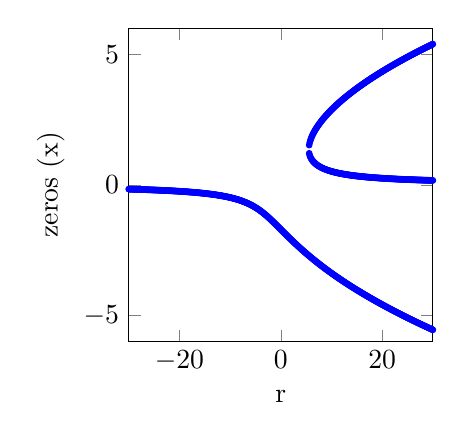
\begin{tikzpicture}

\begin{axis}[%
width=1.520833in,
height=1.565625in,
at={(0.758333in,0.48125in)},
scale only axis,
xmin=-30,
xmax=30,
xlabel={r},
ymin=-6,
ymax=6,
ylabel={zeros (x)}
]
\addplot [color=blue,only marks,mark=*,mark size={1},forget plot]
  table[row sep=crcr]{%
-30	-0.166512772767465\\
};
\addplot [color=blue,only marks,mark=*,mark size={1},forget plot]
  table[row sep=crcr]{%
-29.9	-0.167068121576816\\
};
\addplot [color=blue,only marks,mark=*,mark size={1},forget plot]
  table[row sep=crcr]{%
-29.8	-0.16762717670106\\
};
\addplot [color=blue,only marks,mark=*,mark size={1},forget plot]
  table[row sep=crcr]{%
-29.7	-0.168189975226301\\
};
\addplot [color=blue,only marks,mark=*,mark size={1},forget plot]
  table[row sep=crcr]{%
-29.6	-0.168756554732689\\
};
\addplot [color=blue,only marks,mark=*,mark size={1},forget plot]
  table[row sep=crcr]{%
-29.5	-0.169326953302634\\
};
\addplot [color=blue,only marks,mark=*,mark size={1},forget plot]
  table[row sep=crcr]{%
-29.4	-0.169901209529164\\
};
\addplot [color=blue,only marks,mark=*,mark size={1},forget plot]
  table[row sep=crcr]{%
-29.3	-0.170479362524467\\
};
\addplot [color=blue,only marks,mark=*,mark size={1},forget plot]
  table[row sep=crcr]{%
-29.2	-0.171061451928595\\
};
\addplot [color=blue,only marks,mark=*,mark size={1},forget plot]
  table[row sep=crcr]{%
-29.1	-0.171647517918344\\
};
\addplot [color=blue,only marks,mark=*,mark size={1},forget plot]
  table[row sep=crcr]{%
-29	-0.17223760121631\\
};
\addplot [color=blue,only marks,mark=*,mark size={1},forget plot]
  table[row sep=crcr]{%
-28.9	-0.172831743100136\\
};
\addplot [color=blue,only marks,mark=*,mark size={1},forget plot]
  table[row sep=crcr]{%
-28.8	-0.173429985411935\\
};
\addplot [color=blue,only marks,mark=*,mark size={1},forget plot]
  table[row sep=crcr]{%
-28.7	-0.174032370567911\\
};
\addplot [color=blue,only marks,mark=*,mark size={1},forget plot]
  table[row sep=crcr]{%
-28.6	-0.174638941568175\\
};
\addplot [color=blue,only marks,mark=*,mark size={1},forget plot]
  table[row sep=crcr]{%
-28.5	-0.175249742006763\\
};
\addplot [color=blue,only marks,mark=*,mark size={1},forget plot]
  table[row sep=crcr]{%
-28.4	-0.175864816081851\\
};
\addplot [color=blue,only marks,mark=*,mark size={1},forget plot]
  table[row sep=crcr]{%
-28.3	-0.176484208606195\\
};
\addplot [color=blue,only marks,mark=*,mark size={1},forget plot]
  table[row sep=crcr]{%
-28.2	-0.177107965017768\\
};
\addplot [color=blue,only marks,mark=*,mark size={1},forget plot]
  table[row sep=crcr]{%
-28.1	-0.177736131390634\\
};
\addplot [color=blue,only marks,mark=*,mark size={1},forget plot]
  table[row sep=crcr]{%
-28	-0.178368754446036\\
};
\addplot [color=blue,only marks,mark=*,mark size={1},forget plot]
  table[row sep=crcr]{%
-27.9	-0.179005881563723\\
};
\addplot [color=blue,only marks,mark=*,mark size={1},forget plot]
  table[row sep=crcr]{%
-27.8	-0.179647560793504\\
};
\addplot [color=blue,only marks,mark=*,mark size={1},forget plot]
  table[row sep=crcr]{%
-27.7	-0.180293840867055\\
};
\addplot [color=blue,only marks,mark=*,mark size={1},forget plot]
  table[row sep=crcr]{%
-27.6	-0.180944771209966\\
};
\addplot [color=blue,only marks,mark=*,mark size={1},forget plot]
  table[row sep=crcr]{%
-27.5	-0.181600401954048\\
};
\addplot [color=blue,only marks,mark=*,mark size={1},forget plot]
  table[row sep=crcr]{%
-27.4	-0.182260783949893\\
};
\addplot [color=blue,only marks,mark=*,mark size={1},forget plot]
  table[row sep=crcr]{%
-27.3	-0.182925968779713\\
};
\addplot [color=blue,only marks,mark=*,mark size={1},forget plot]
  table[row sep=crcr]{%
-27.2	-0.183596008770435\\
};
\addplot [color=blue,only marks,mark=*,mark size={1},forget plot]
  table[row sep=crcr]{%
-27.1	-0.184270957007094\\
};
\addplot [color=blue,only marks,mark=*,mark size={1},forget plot]
  table[row sep=crcr]{%
-27	-0.184950867346501\\
};
\addplot [color=blue,only marks,mark=*,mark size={1},forget plot]
  table[row sep=crcr]{%
-26.9	-0.185635794431211\\
};
\addplot [color=blue,only marks,mark=*,mark size={1},forget plot]
  table[row sep=crcr]{%
-26.8	-0.186325793703788\\
};
\addplot [color=blue,only marks,mark=*,mark size={1},forget plot]
  table[row sep=crcr]{%
-26.7	-0.187020921421381\\
};
\addplot [color=blue,only marks,mark=*,mark size={1},forget plot]
  table[row sep=crcr]{%
-26.6	-0.187721234670623\\
};
\addplot [color=blue,only marks,mark=*,mark size={1},forget plot]
  table[row sep=crcr]{%
-26.5	-0.18842679138284\\
};
\addplot [color=blue,only marks,mark=*,mark size={1},forget plot]
  table[row sep=crcr]{%
-26.4	-0.189137650349609\\
};
\addplot [color=blue,only marks,mark=*,mark size={1},forget plot]
  table[row sep=crcr]{%
-26.3	-0.189853871238647\\
};
\addplot [color=blue,only marks,mark=*,mark size={1},forget plot]
  table[row sep=crcr]{%
-26.2	-0.190575514610053\\
};
\addplot [color=blue,only marks,mark=*,mark size={1},forget plot]
  table[row sep=crcr]{%
-26.1	-0.191302641932909\\
};
\addplot [color=blue,only marks,mark=*,mark size={1},forget plot]
  table[row sep=crcr]{%
-26	-0.19203531560225\\
};
\addplot [color=blue,only marks,mark=*,mark size={1},forget plot]
  table[row sep=crcr]{%
-25.9	-0.192773598956408\\
};
\addplot [color=blue,only marks,mark=*,mark size={1},forget plot]
  table[row sep=crcr]{%
-25.8	-0.19351755629475\\
};
\addplot [color=blue,only marks,mark=*,mark size={1},forget plot]
  table[row sep=crcr]{%
-25.7	-0.194267252895802\\
};
\addplot [color=blue,only marks,mark=*,mark size={1},forget plot]
  table[row sep=crcr]{%
-25.6	-0.195022755035796\\
};
\addplot [color=blue,only marks,mark=*,mark size={1},forget plot]
  table[row sep=crcr]{%
-25.5	-0.195784130007617\\
};
\addplot [color=blue,only marks,mark=*,mark size={1},forget plot]
  table[row sep=crcr]{%
-25.4	-0.196551446140195\\
};
\addplot [color=blue,only marks,mark=*,mark size={1},forget plot]
  table[row sep=crcr]{%
-25.3	-0.197324772818328\\
};
\addplot [color=blue,only marks,mark=*,mark size={1},forget plot]
  table[row sep=crcr]{%
-25.2	-0.198104180502958\\
};
\addplot [color=blue,only marks,mark=*,mark size={1},forget plot]
  table[row sep=crcr]{%
-25.1	-0.198889740751912\\
};
\addplot [color=blue,only marks,mark=*,mark size={1},forget plot]
  table[row sep=crcr]{%
-25	-0.199681526241122\\
};
\addplot [color=blue,only marks,mark=*,mark size={1},forget plot]
  table[row sep=crcr]{%
-24.9	-0.200479610786322\\
};
\addplot [color=blue,only marks,mark=*,mark size={1},forget plot]
  table[row sep=crcr]{%
-24.8	-0.201284069365261\\
};
\addplot [color=blue,only marks,mark=*,mark size={1},forget plot]
  table[row sep=crcr]{%
-24.7	-0.20209497814042\\
};
\addplot [color=blue,only marks,mark=*,mark size={1},forget plot]
  table[row sep=crcr]{%
-24.6	-0.202912414482264\\
};
\addplot [color=blue,only marks,mark=*,mark size={1},forget plot]
  table[row sep=crcr]{%
-24.5	-0.20373645699303\\
};
\addplot [color=blue,only marks,mark=*,mark size={1},forget plot]
  table[row sep=crcr]{%
-24.4	-0.204567185531078\\
};
\addplot [color=blue,only marks,mark=*,mark size={1},forget plot]
  table[row sep=crcr]{%
-24.3	-0.205404681235814\\
};
\addplot [color=blue,only marks,mark=*,mark size={1},forget plot]
  table[row sep=crcr]{%
-24.2	-0.206249026553196\\
};
\addplot [color=blue,only marks,mark=*,mark size={1},forget plot]
  table[row sep=crcr]{%
-24.1	-0.207100305261848\\
};
\addplot [color=blue,only marks,mark=*,mark size={1},forget plot]
  table[row sep=crcr]{%
-24	-0.207958602499793\\
};
\addplot [color=blue,only marks,mark=*,mark size={1},forget plot]
  table[row sep=crcr]{%
-23.9	-0.208824004791825\\
};
\addplot [color=blue,only marks,mark=*,mark size={1},forget plot]
  table[row sep=crcr]{%
-23.8	-0.20969660007753\\
};
\addplot [color=blue,only marks,mark=*,mark size={1},forget plot]
  table[row sep=crcr]{%
-23.7	-0.210576477739986\\
};
\addplot [color=blue,only marks,mark=*,mark size={1},forget plot]
  table[row sep=crcr]{%
-23.6	-0.211463728635151\\
};
\addplot [color=blue,only marks,mark=*,mark size={1},forget plot]
  table[row sep=crcr]{%
-23.5	-0.212358445121963\\
};
\addplot [color=blue,only marks,mark=*,mark size={1},forget plot]
  table[row sep=crcr]{%
-23.4	-0.213260721093167\\
};
\addplot [color=blue,only marks,mark=*,mark size={1},forget plot]
  table[row sep=crcr]{%
-23.3	-0.214170652006898\\
};
\addplot [color=blue,only marks,mark=*,mark size={1},forget plot]
  table[row sep=crcr]{%
-23.2	-0.215088334919028\\
};
\addplot [color=blue,only marks,mark=*,mark size={1},forget plot]
  table[row sep=crcr]{%
-23.1	-0.216013868516315\\
};
\addplot [color=blue,only marks,mark=*,mark size={1},forget plot]
  table[row sep=crcr]{%
-23	-0.21694735315036\\
};
\addplot [color=blue,only marks,mark=*,mark size={1},forget plot]
  table[row sep=crcr]{%
-22.9	-0.217888890872407\\
};
\addplot [color=blue,only marks,mark=*,mark size={1},forget plot]
  table[row sep=crcr]{%
-22.8	-0.218838585469003\\
};
\addplot [color=blue,only marks,mark=*,mark size={1},forget plot]
  table[row sep=crcr]{%
-22.7	-0.219796542498545\\
};
\addplot [color=blue,only marks,mark=*,mark size={1},forget plot]
  table[row sep=crcr]{%
-22.6	-0.220762869328741\\
};
\addplot [color=blue,only marks,mark=*,mark size={1},forget plot]
  table[row sep=crcr]{%
-22.5	-0.221737675175011\\
};
\addplot [color=blue,only marks,mark=*,mark size={1},forget plot]
  table[row sep=crcr]{%
-22.4	-0.222721071139843\\
};
\addplot [color=blue,only marks,mark=*,mark size={1},forget plot]
  table[row sep=crcr]{%
-22.3	-0.223713170253158\\
};
\addplot [color=blue,only marks,mark=*,mark size={1},forget plot]
  table[row sep=crcr]{%
-22.2	-0.224714087513681\\
};
\addplot [color=blue,only marks,mark=*,mark size={1},forget plot]
  table[row sep=crcr]{%
-22.1	-0.225723939931377\\
};
\addplot [color=blue,only marks,mark=*,mark size={1},forget plot]
  table[row sep=crcr]{%
-22	-0.226742846570957\\
};
\addplot [color=blue,only marks,mark=*,mark size={1},forget plot]
  table[row sep=crcr]{%
-21.9	-0.227770928596508\\
};
\addplot [color=blue,only marks,mark=*,mark size={1},forget plot]
  table[row sep=crcr]{%
-21.8	-0.228808309317261\\
};
\addplot [color=blue,only marks,mark=*,mark size={1},forget plot]
  table[row sep=crcr]{%
-21.7	-0.229855114234545\\
};
\addplot [color=blue,only marks,mark=*,mark size={1},forget plot]
  table[row sep=crcr]{%
-21.6	-0.230911471089949\\
};
\addplot [color=blue,only marks,mark=*,mark size={1},forget plot]
  table[row sep=crcr]{%
-21.5	-0.231977509914745\\
};
\addplot [color=blue,only marks,mark=*,mark size={1},forget plot]
  table[row sep=crcr]{%
-21.4	-0.233053363080585\\
};
\addplot [color=blue,only marks,mark=*,mark size={1},forget plot]
  table[row sep=crcr]{%
-21.3	-0.234139165351536\\
};
\addplot [color=blue,only marks,mark=*,mark size={1},forget plot]
  table[row sep=crcr]{%
-21.2	-0.235235053937473\\
};
\addplot [color=blue,only marks,mark=*,mark size={1},forget plot]
  table[row sep=crcr]{%
-21.1	-0.236341168548883\\
};
\addplot [color=blue,only marks,mark=*,mark size={1},forget plot]
  table[row sep=crcr]{%
-21	-0.237457651453117\\
};
\addplot [color=blue,only marks,mark=*,mark size={1},forget plot]
  table[row sep=crcr]{%
-20.9	-0.238584647532126\\
};
\addplot [color=blue,only marks,mark=*,mark size={1},forget plot]
  table[row sep=crcr]{%
-20.8	-0.239722304341752\\
};
\addplot [color=blue,only marks,mark=*,mark size={1},forget plot]
  table[row sep=crcr]{%
-20.7	-0.240870772172585\\
};
\addplot [color=blue,only marks,mark=*,mark size={1},forget plot]
  table[row sep=crcr]{%
-20.6	-0.242030204112462\\
};
\addplot [color=blue,only marks,mark=*,mark size={1},forget plot]
  table[row sep=crcr]{%
-20.5	-0.243200756110648\\
};
\addplot [color=blue,only marks,mark=*,mark size={1},forget plot]
  table[row sep=crcr]{%
-20.4	-0.244382587043743\\
};
\addplot [color=blue,only marks,mark=*,mark size={1},forget plot]
  table[row sep=crcr]{%
-20.3	-0.24557585878339\\
};
\addplot [color=blue,only marks,mark=*,mark size={1},forget plot]
  table[row sep=crcr]{%
-20.2	-0.246780736265805\\
};
\addplot [color=blue,only marks,mark=*,mark size={1},forget plot]
  table[row sep=crcr]{%
-20.1	-0.247997387563227\\
};
\addplot [color=blue,only marks,mark=*,mark size={1},forget plot]
  table[row sep=crcr]{%
-20	-0.249225983957305\\
};
\addplot [color=blue,only marks,mark=*,mark size={1},forget plot]
  table[row sep=crcr]{%
-19.9	-0.25046670001452\\
};
\addplot [color=blue,only marks,mark=*,mark size={1},forget plot]
  table[row sep=crcr]{%
-19.8	-0.251719713663679\\
};
\addplot [color=blue,only marks,mark=*,mark size={1},forget plot]
  table[row sep=crcr]{%
-19.7	-0.252985206275554\\
};
\addplot [color=blue,only marks,mark=*,mark size={1},forget plot]
  table[row sep=crcr]{%
-19.6	-0.254263362744742\\
};
\addplot [color=blue,only marks,mark=*,mark size={1},forget plot]
  table[row sep=crcr]{%
-19.5	-0.255554371573798\\
};
\addplot [color=blue,only marks,mark=*,mark size={1},forget plot]
  table[row sep=crcr]{%
-19.4	-0.256858424959732\\
};
\addplot [color=blue,only marks,mark=*,mark size={1},forget plot]
  table[row sep=crcr]{%
-19.3	-0.258175718882928\\
};
\addplot [color=blue,only marks,mark=*,mark size={1},forget plot]
  table[row sep=crcr]{%
-19.2	-0.259506453198571\\
};
\addplot [color=blue,only marks,mark=*,mark size={1},forget plot]
  table[row sep=crcr]{%
-19.1	-0.260850831730664\\
};
\addplot [color=blue,only marks,mark=*,mark size={1},forget plot]
  table[row sep=crcr]{%
-19	-0.262209062368705\\
};
\addplot [color=blue,only marks,mark=*,mark size={1},forget plot]
  table[row sep=crcr]{%
-18.9	-0.263581357167124\\
};
\addplot [color=blue,only marks,mark=*,mark size={1},forget plot]
  table[row sep=crcr]{%
-18.8	-0.26496793244756\\
};
\addplot [color=blue,only marks,mark=*,mark size={1},forget plot]
  table[row sep=crcr]{%
-18.7	-0.266369008904063\\
};
\addplot [color=blue,only marks,mark=*,mark size={1},forget plot]
  table[row sep=crcr]{%
-18.6	-0.267784811711337\\
};
\addplot [color=blue,only marks,mark=*,mark size={1},forget plot]
  table[row sep=crcr]{%
-18.5	-0.269215570636094\\
};
\addplot [color=blue,only marks,mark=*,mark size={1},forget plot]
  table[row sep=crcr]{%
-18.4	-0.270661520151638\\
};
\addplot [color=blue,only marks,mark=*,mark size={1},forget plot]
  table[row sep=crcr]{%
-18.3	-0.272122899555783\\
};
\addplot [color=blue,only marks,mark=*,mark size={1},forget plot]
  table[row sep=crcr]{%
-18.2	-0.273599953092205\\
};
\addplot [color=blue,only marks,mark=*,mark size={1},forget plot]
  table[row sep=crcr]{%
-18.1	-0.27509293007534\\
};
\addplot [color=blue,only marks,mark=*,mark size={1},forget plot]
  table[row sep=crcr]{%
-18	-0.276602085018959\\
};
\addplot [color=blue,only marks,mark=*,mark size={1},forget plot]
  table[row sep=crcr]{%
-17.9	-0.278127677768513\\
};
\addplot [color=blue,only marks,mark=*,mark size={1},forget plot]
  table[row sep=crcr]{%
-17.8	-0.279669973637405\\
};
\addplot [color=blue,only marks,mark=*,mark size={1},forget plot]
  table[row sep=crcr]{%
-17.7	-0.281229243547282\\
};
\addplot [color=blue,only marks,mark=*,mark size={1},forget plot]
  table[row sep=crcr]{%
-17.6	-0.282805764172511\\
};
\addplot [color=blue,only marks,mark=*,mark size={1},forget plot]
  table[row sep=crcr]{%
-17.5	-0.284399818088954\\
};
\addplot [color=blue,only marks,mark=*,mark size={1},forget plot]
  table[row sep=crcr]{%
-17.4	-0.286011693927199\\
};
\addplot [color=blue,only marks,mark=*,mark size={1},forget plot]
  table[row sep=crcr]{%
-17.3	-0.28764168653038\\
};
\addplot [color=blue,only marks,mark=*,mark size={1},forget plot]
  table[row sep=crcr]{%
-17.2	-0.289290097116755\\
};
\addplot [color=blue,only marks,mark=*,mark size={1},forget plot]
  table[row sep=crcr]{%
-17.1	-0.290957233447179\\
};
\addplot [color=blue,only marks,mark=*,mark size={1},forget plot]
  table[row sep=crcr]{%
-17	-0.292643409997657\\
};
\addplot [color=blue,only marks,mark=*,mark size={1},forget plot]
  table[row sep=crcr]{%
-16.9	-0.294348948137125\\
};
\addplot [color=blue,only marks,mark=*,mark size={1},forget plot]
  table[row sep=crcr]{%
-16.8	-0.296074176310643\\
};
\addplot [color=blue,only marks,mark=*,mark size={1},forget plot]
  table[row sep=crcr]{%
-16.7	-0.297819430228184\\
};
\addplot [color=blue,only marks,mark=*,mark size={1},forget plot]
  table[row sep=crcr]{%
-16.6	-0.299585053059193\\
};
\addplot [color=blue,only marks,mark=*,mark size={1},forget plot]
  table[row sep=crcr]{%
-16.5	-0.301371395633118\\
};
\addplot [color=blue,only marks,mark=*,mark size={1},forget plot]
  table[row sep=crcr]{%
-16.4	-0.303178816646114\\
};
\addplot [color=blue,only marks,mark=*,mark size={1},forget plot]
  table[row sep=crcr]{%
-16.3	-0.305007682874104\\
};
\addplot [color=blue,only marks,mark=*,mark size={1},forget plot]
  table[row sep=crcr]{%
-16.2	-0.30685836939245\\
};
\addplot [color=blue,only marks,mark=*,mark size={1},forget plot]
  table[row sep=crcr]{%
-16.1	-0.308731259802403\\
};
\addplot [color=blue,only marks,mark=*,mark size={1},forget plot]
  table[row sep=crcr]{%
-16	-0.310626746464607\\
};
\addplot [color=blue,only marks,mark=*,mark size={1},forget plot]
  table[row sep=crcr]{%
-15.9	-0.312545230739851\\
};
\addplot [color=blue,only marks,mark=*,mark size={1},forget plot]
  table[row sep=crcr]{%
-15.8	-0.314487123237342\\
};
\addplot [color=blue,only marks,mark=*,mark size={1},forget plot]
  table[row sep=crcr]{%
-15.7	-0.316452844070722\\
};
\addplot [color=blue,only marks,mark=*,mark size={1},forget plot]
  table[row sep=crcr]{%
-15.6	-0.318442823122109\\
};
\addplot [color=blue,only marks,mark=*,mark size={1},forget plot]
  table[row sep=crcr]{%
-15.5	-0.320457500314412\\
};
\addplot [color=blue,only marks,mark=*,mark size={1},forget plot]
  table[row sep=crcr]{%
-15.4	-0.322497325892198\\
};
\addplot [color=blue,only marks,mark=*,mark size={1},forget plot]
  table[row sep=crcr]{%
-15.3	-0.3245627607114\\
};
\addplot [color=blue,only marks,mark=*,mark size={1},forget plot]
  table[row sep=crcr]{%
-15.2	-0.326654276538141\\
};
\addplot [color=blue,only marks,mark=*,mark size={1},forget plot]
  table[row sep=crcr]{%
-15.1	-0.328772356356989\\
};
\addplot [color=blue,only marks,mark=*,mark size={1},forget plot]
  table[row sep=crcr]{%
-15	-0.330917494688949\\
};
\addplot [color=blue,only marks,mark=*,mark size={1},forget plot]
  table[row sep=crcr]{%
-14.9	-0.333090197919494\\
};
\addplot [color=blue,only marks,mark=*,mark size={1},forget plot]
  table[row sep=crcr]{%
-14.8	-0.335290984636979\\
};
\addplot [color=blue,only marks,mark=*,mark size={1},forget plot]
  table[row sep=crcr]{%
-14.7	-0.337520385981769\\
};
\addplot [color=blue,only marks,mark=*,mark size={1},forget plot]
  table[row sep=crcr]{%
-14.6	-0.339778946006412\\
};
\addplot [color=blue,only marks,mark=*,mark size={1},forget plot]
  table[row sep=crcr]{%
-14.5	-0.342067222047228\\
};
\addplot [color=blue,only marks,mark=*,mark size={1},forget plot]
  table[row sep=crcr]{%
-14.4	-0.344385785107664\\
};
\addplot [color=blue,only marks,mark=*,mark size={1},forget plot]
  table[row sep=crcr]{%
-14.3	-0.34673522025379\\
};
\addplot [color=blue,only marks,mark=*,mark size={1},forget plot]
  table[row sep=crcr]{%
-14.2	-0.34911612702231\\
};
\addplot [color=blue,only marks,mark=*,mark size={1},forget plot]
  table[row sep=crcr]{%
-14.1	-0.351529119841489\\
};
\addplot [color=blue,only marks,mark=*,mark size={1},forget plot]
  table[row sep=crcr]{%
-14	-0.353974828465373\\
};
\addplot [color=blue,only marks,mark=*,mark size={1},forget plot]
  table[row sep=crcr]{%
-13.9	-0.356453898421724\\
};
\addplot [color=blue,only marks,mark=*,mark size={1},forget plot]
  table[row sep=crcr]{%
-13.8	-0.358966991474063\\
};
\addplot [color=blue,only marks,mark=*,mark size={1},forget plot]
  table[row sep=crcr]{%
-13.7	-0.361514786098257\\
};
\addplot [color=blue,only marks,mark=*,mark size={1},forget plot]
  table[row sep=crcr]{%
-13.6	-0.364097977974063\\
};
\addplot [color=blue,only marks,mark=*,mark size={1},forget plot]
  table[row sep=crcr]{%
-13.5	-0.366717280492054\\
};
\addplot [color=blue,only marks,mark=*,mark size={1},forget plot]
  table[row sep=crcr]{%
-13.4	-0.369373425276384\\
};
\addplot [color=blue,only marks,mark=*,mark size={1},forget plot]
  table[row sep=crcr]{%
-13.3	-0.372067162723797\\
};
\addplot [color=blue,only marks,mark=*,mark size={1},forget plot]
  table[row sep=crcr]{%
-13.2	-0.374799262559349\\
};
\addplot [color=blue,only marks,mark=*,mark size={1},forget plot]
  table[row sep=crcr]{%
-13.1	-0.37757051440927\\
};
\addplot [color=blue,only marks,mark=*,mark size={1},forget plot]
  table[row sep=crcr]{%
-13	-0.38038172839141\\
};
\addplot [color=blue,only marks,mark=*,mark size={1},forget plot]
  table[row sep=crcr]{%
-12.9	-0.383233735723712\\
};
\addplot [color=blue,only marks,mark=*,mark size={1},forget plot]
  table[row sep=crcr]{%
-12.8	-0.386127389351138\\
};
\addplot [color=blue,only marks,mark=*,mark size={1},forget plot]
  table[row sep=crcr]{%
-12.7	-0.389063564591487\\
};
\addplot [color=blue,only marks,mark=*,mark size={1},forget plot]
  table[row sep=crcr]{%
-12.6	-0.392043159800519\\
};
\addplot [color=blue,only marks,mark=*,mark size={1},forget plot]
  table[row sep=crcr]{%
-12.5	-0.395067097056796\\
};
\addplot [color=blue,only marks,mark=*,mark size={1},forget plot]
  table[row sep=crcr]{%
-12.4	-0.398136322866626\\
};
\addplot [color=blue,only marks,mark=*,mark size={1},forget plot]
  table[row sep=crcr]{%
-12.3	-0.401251808889498\\
};
\addplot [color=blue,only marks,mark=*,mark size={1},forget plot]
  table[row sep=crcr]{%
-12.2	-0.404414552684345\\
};
\addplot [color=blue,only marks,mark=*,mark size={1},forget plot]
  table[row sep=crcr]{%
-12.1	-0.407625578476971\\
};
\addplot [color=blue,only marks,mark=*,mark size={1},forget plot]
  table[row sep=crcr]{%
-12	-0.410885937948929\\
};
\addplot [color=blue,only marks,mark=*,mark size={1},forget plot]
  table[row sep=crcr]{%
-11.9	-0.414196711048109\\
};
\addplot [color=blue,only marks,mark=*,mark size={1},forget plot]
  table[row sep=crcr]{%
-11.8	-0.41755900682124\\
};
\addplot [color=blue,only marks,mark=*,mark size={1},forget plot]
  table[row sep=crcr]{%
-11.7	-0.420973964268475\\
};
\addplot [color=blue,only marks,mark=*,mark size={1},forget plot]
  table[row sep=crcr]{%
-11.6	-0.424442753220155\\
};
\addplot [color=blue,only marks,mark=*,mark size={1},forget plot]
  table[row sep=crcr]{%
-11.5	-0.427966575235787\\
};
\addplot [color=blue,only marks,mark=*,mark size={1},forget plot]
  table[row sep=crcr]{%
-11.4	-0.431546664525193\\
};
\addplot [color=blue,only marks,mark=*,mark size={1},forget plot]
  table[row sep=crcr]{%
-11.3	-0.435184288891701\\
};
\addplot [color=blue,only marks,mark=*,mark size={1},forget plot]
  table[row sep=crcr]{%
-11.2	-0.438880750697153\\
};
\addplot [color=blue,only marks,mark=*,mark size={1},forget plot]
  table[row sep=crcr]{%
-11.1	-0.442637387848389\\
};
\addplot [color=blue,only marks,mark=*,mark size={1},forget plot]
  table[row sep=crcr]{%
-11	-0.446455574804737\\
};
\addplot [color=blue,only marks,mark=*,mark size={1},forget plot]
  table[row sep=crcr]{%
-10.9	-0.450336723605914\\
};
\addplot [color=blue,only marks,mark=*,mark size={1},forget plot]
  table[row sep=crcr]{%
-10.8	-0.454282284919574\\
};
\addplot [color=blue,only marks,mark=*,mark size={1},forget plot]
  table[row sep=crcr]{%
-10.7	-0.458293749107552\\
};
\addplot [color=blue,only marks,mark=*,mark size={1},forget plot]
  table[row sep=crcr]{%
-10.6	-0.462372647309702\\
};
\addplot [color=blue,only marks,mark=*,mark size={1},forget plot]
  table[row sep=crcr]{%
-10.5	-0.466520552543931\\
};
\addplot [color=blue,only marks,mark=*,mark size={1},forget plot]
  table[row sep=crcr]{%
-10.4	-0.470739080820888\\
};
\addplot [color=blue,only marks,mark=*,mark size={1},forget plot]
  table[row sep=crcr]{%
-10.3	-0.475029892271404\\
};
\addplot [color=blue,only marks,mark=*,mark size={1},forget plot]
  table[row sep=crcr]{%
-10.2	-0.479394692284549\\
};
\addplot [color=blue,only marks,mark=*,mark size={1},forget plot]
  table[row sep=crcr]{%
-10.1	-0.483835232653814\\
};
\addplot [color=blue,only marks,mark=*,mark size={1},forget plot]
  table[row sep=crcr]{%
-10	-0.488353312728565\\
};
\addplot [color=blue,only marks,mark=*,mark size={1},forget plot]
  table[row sep=crcr]{%
-9.9	-0.492950780567544\\
};
\addplot [color=blue,only marks,mark=*,mark size={1},forget plot]
  table[row sep=crcr]{%
-9.8	-0.497629534090708\\
};
\addplot [color=blue,only marks,mark=*,mark size={1},forget plot]
  table[row sep=crcr]{%
-9.7	-0.502391522225277\\
};
\addplot [color=blue,only marks,mark=*,mark size={1},forget plot]
  table[row sep=crcr]{%
-9.6	-0.50723874604129\\
};
\addplot [color=blue,only marks,mark=*,mark size={1},forget plot]
  table[row sep=crcr]{%
-9.5	-0.512173259871415\\
};
\addplot [color=blue,only marks,mark=*,mark size={1},forget plot]
  table[row sep=crcr]{%
-9.4	-0.517197172409145\\
};
\addplot [color=blue,only marks,mark=*,mark size={1},forget plot]
  table[row sep=crcr]{%
-9.3	-0.522312647778816\\
};
\addplot [color=blue,only marks,mark=*,mark size={1},forget plot]
  table[row sep=crcr]{%
-9.2	-0.527521906570149\\
};
\addplot [color=blue,only marks,mark=*,mark size={1},forget plot]
  table[row sep=crcr]{%
-9.1	-0.532827226829234\\
};
\addplot [color=blue,only marks,mark=*,mark size={1},forget plot]
  table[row sep=crcr]{%
-9	-0.53823094499699\\
};
\addplot [color=blue,only marks,mark=*,mark size={1},forget plot]
  table[row sep=crcr]{%
-8.9	-0.543735456785224\\
};
\addplot [color=blue,only marks,mark=*,mark size={1},forget plot]
  table[row sep=crcr]{%
-8.8	-0.549343217979396\\
};
\addplot [color=blue,only marks,mark=*,mark size={1},forget plot]
  table[row sep=crcr]{%
-8.7	-0.555056745156131\\
};
\addplot [color=blue,only marks,mark=*,mark size={1},forget plot]
  table[row sep=crcr]{%
-8.6	-0.56087861630239\\
};
\addplot [color=blue,only marks,mark=*,mark size={1},forget plot]
  table[row sep=crcr]{%
-8.5	-0.566811471321941\\
};
\addplot [color=blue,only marks,mark=*,mark size={1},forget plot]
  table[row sep=crcr]{%
-8.4	-0.57285801241355\\
};
\addplot [color=blue,only marks,mark=*,mark size={1},forget plot]
  table[row sep=crcr]{%
-8.3	-0.579021004303874\\
};
\addplot [color=blue,only marks,mark=*,mark size={1},forget plot]
  table[row sep=crcr]{%
-8.2	-0.585303274316635\\
};
\addplot [color=blue,only marks,mark=*,mark size={1},forget plot]
  table[row sep=crcr]{%
-8.1	-0.591707712258148\\
};
\addplot [color=blue,only marks,mark=*,mark size={1},forget plot]
  table[row sep=crcr]{%
-8	-0.598237270097699\\
};
\addplot [color=blue,only marks,mark=*,mark size={1},forget plot]
  table[row sep=crcr]{%
-7.9	-0.604894961419646\\
};
\addplot [color=blue,only marks,mark=*,mark size={1},forget plot]
  table[row sep=crcr]{%
-7.8	-0.611683860622471\\
};
\addplot [color=blue,only marks,mark=*,mark size={1},forget plot]
  table[row sep=crcr]{%
-7.7	-0.61860710183832\\
};
\addplot [color=blue,only marks,mark=*,mark size={1},forget plot]
  table[row sep=crcr]{%
-7.6	-0.625667877544859\\
};
\addplot [color=blue,only marks,mark=*,mark size={1},forget plot]
  table[row sep=crcr]{%
-7.5	-0.6328694368396\\
};
\addplot [color=blue,only marks,mark=*,mark size={1},forget plot]
  table[row sep=crcr]{%
-7.4	-0.640215083345219\\
};
\addplot [color=blue,only marks,mark=*,mark size={1},forget plot]
  table[row sep=crcr]{%
-7.3	-0.64770817271278\\
};
\addplot [color=blue,only marks,mark=*,mark size={1},forget plot]
  table[row sep=crcr]{%
-7.2	-0.655352109688346\\
};
\addplot [color=blue,only marks,mark=*,mark size={1},forget plot]
  table[row sep=crcr]{%
-7.1	-0.663150344707112\\
};
\addplot [color=blue,only marks,mark=*,mark size={1},forget plot]
  table[row sep=crcr]{%
-7	-0.671106369978092\\
};
\addplot [color=blue,only marks,mark=*,mark size={1},forget plot]
  table[row sep=crcr]{%
-6.9	-0.679223715021519\\
};
\addplot [color=blue,only marks,mark=*,mark size={1},forget plot]
  table[row sep=crcr]{%
-6.8	-0.687505941620572\\
};
\addplot [color=blue,only marks,mark=*,mark size={1},forget plot]
  table[row sep=crcr]{%
-6.7	-0.695956638148885\\
};
\addplot [color=blue,only marks,mark=*,mark size={1},forget plot]
  table[row sep=crcr]{%
-6.6	-0.704579413235599\\
};
\addplot [color=blue,only marks,mark=*,mark size={1},forget plot]
  table[row sep=crcr]{%
-6.5	-0.713377888730588\\
};
\addplot [color=blue,only marks,mark=*,mark size={1},forget plot]
  table[row sep=crcr]{%
-6.4	-0.722355691933968\\
};
\addplot [color=blue,only marks,mark=*,mark size={1},forget plot]
  table[row sep=crcr]{%
-6.3	-0.731516447056249\\
};
\addplot [color=blue,only marks,mark=*,mark size={1},forget plot]
  table[row sep=crcr]{%
-6.2	-0.740863765878569\\
};
\addplot [color=blue,only marks,mark=*,mark size={1},forget plot]
  table[row sep=crcr]{%
-6.1	-0.750401237586427\\
};
\addplot [color=blue,only marks,mark=*,mark size={1},forget plot]
  table[row sep=crcr]{%
-6	-0.760132417755419\\
};
\addplot [color=blue,only marks,mark=*,mark size={1},forget plot]
  table[row sep=crcr]{%
-5.9	-0.77006081647361\\
};
\addplot [color=blue,only marks,mark=*,mark size={1},forget plot]
  table[row sep=crcr]{%
-5.8	-0.780189885592621\\
};
\addplot [color=blue,only marks,mark=*,mark size={1},forget plot]
  table[row sep=crcr]{%
-5.7	-0.790523005108164\\
};
\addplot [color=blue,only marks,mark=*,mark size={1},forget plot]
  table[row sep=crcr]{%
-5.6	-0.801063468680815\\
};
\addplot [color=blue,only marks,mark=*,mark size={1},forget plot]
  table[row sep=crcr]{%
-5.5	-0.811814468319256\\
};
\addplot [color=blue,only marks,mark=*,mark size={1},forget plot]
  table[row sep=crcr]{%
-5.4	-0.822779078261001\\
};
\addplot [color=blue,only marks,mark=*,mark size={1},forget plot]
  table[row sep=crcr]{%
-5.3	-0.833960238099828\\
};
\addplot [color=blue,only marks,mark=*,mark size={1},forget plot]
  table[row sep=crcr]{%
-5.2	-0.845360735224546\\
};
\addplot [color=blue,only marks,mark=*,mark size={1},forget plot]
  table[row sep=crcr]{%
-5.1	-0.856983186650342\\
};
\addplot [color=blue,only marks,mark=*,mark size={1},forget plot]
  table[row sep=crcr]{%
-5	-0.868830020341475\\
};
\addplot [color=blue,only marks,mark=*,mark size={1},forget plot]
  table[row sep=crcr]{%
-4.9	-0.880903456142354\\
};
\addplot [color=blue,only marks,mark=*,mark size={1},forget plot]
  table[row sep=crcr]{%
-4.8	-0.89320548645267\\
};
\addplot [color=blue,only marks,mark=*,mark size={1},forget plot]
  table[row sep=crcr]{%
-4.7	-0.905737856800944\\
};
\addplot [color=blue,only marks,mark=*,mark size={1},forget plot]
  table[row sep=crcr]{%
-4.6	-0.918502046489043\\
};
\addplot [color=blue,only marks,mark=*,mark size={1},forget plot]
  table[row sep=crcr]{%
-4.5	-0.93149924949754\\
};
\addplot [color=blue,only marks,mark=*,mark size={1},forget plot]
  table[row sep=crcr]{%
-4.4	-0.944730355857585\\
};
\addplot [color=blue,only marks,mark=*,mark size={1},forget plot]
  table[row sep=crcr]{%
-4.3	-0.958195933708624\\
};
\addplot [color=blue,only marks,mark=*,mark size={1},forget plot]
  table[row sep=crcr]{%
-4.2	-0.971896212272329\\
};
\addplot [color=blue,only marks,mark=*,mark size={1},forget plot]
  table[row sep=crcr]{%
-4.1	-0.985831065980693\\
};
\addplot [color=blue,only marks,mark=*,mark size={1},forget plot]
  table[row sep=crcr]{%
-4	-1\\
};
\addplot [color=blue,only marks,mark=*,mark size={1},forget plot]
  table[row sep=crcr]{%
-3.9	-1.01440213739157\\
};
\addplot [color=blue,only marks,mark=*,mark size={1},forget plot]
  table[row sep=crcr]{%
-3.8	-1.02903620814449\\
};
\addplot [color=blue,only marks,mark=*,mark size={1},forget plot]
  table[row sep=crcr]{%
-3.7	-1.04390054030448\\
};
\addplot [color=blue,only marks,mark=*,mark size={1},forget plot]
  table[row sep=crcr]{%
-3.6	-1.05899305340667\\
};
\addplot [color=blue,only marks,mark=*,mark size={1},forget plot]
  table[row sep=crcr]{%
-3.5	-1.07431125439768\\
};
\addplot [color=blue,only marks,mark=*,mark size={1},forget plot]
  table[row sep=crcr]{%
-3.4	-1.08985223620545\\
};
\addplot [color=blue,only marks,mark=*,mark size={1},forget plot]
  table[row sep=crcr]{%
-3.3	-1.10561267908212\\
};
\addplot [color=blue,only marks,mark=*,mark size={1},forget plot]
  table[row sep=crcr]{%
-3.2	-1.12158885480881\\
};
\addplot [color=blue,only marks,mark=*,mark size={1},forget plot]
  table[row sep=crcr]{%
-3.1	-1.13777663380997\\
};
\addplot [color=blue,only marks,mark=*,mark size={1},forget plot]
  table[row sep=crcr]{%
-3	-1.15417149518144\\
};
\addplot [color=blue,only marks,mark=*,mark size={1},forget plot]
  table[row sep=crcr]{%
-2.9	-1.1707685395912\\
};
\addplot [color=blue,only marks,mark=*,mark size={1},forget plot]
  table[row sep=crcr]{%
-2.8	-1.18756250496548\\
};
\addplot [color=blue,only marks,mark=*,mark size={1},forget plot]
  table[row sep=crcr]{%
-2.7	-1.20454778482799\\
};
\addplot [color=blue,only marks,mark=*,mark size={1},forget plot]
  table[row sep=crcr]{%
-2.6	-1.22171844911662\\
};
\addplot [color=blue,only marks,mark=*,mark size={1},forget plot]
  table[row sep=crcr]{%
-2.5	-1.23906826726191\\
};
\addplot [color=blue,only marks,mark=*,mark size={1},forget plot]
  table[row sep=crcr]{%
-2.4	-1.25659073327606\\
};
\addplot [color=blue,only marks,mark=*,mark size={1},forget plot]
  table[row sep=crcr]{%
-2.3	-1.27427909257071\\
};
\addplot [color=blue,only marks,mark=*,mark size={1},forget plot]
  table[row sep=crcr]{%
-2.2	-1.29212637019776\\
};
\addplot [color=blue,only marks,mark=*,mark size={1},forget plot]
  table[row sep=crcr]{%
-2.1	-1.31012540019011\\
};
\addplot [color=blue,only marks,mark=*,mark size={1},forget plot]
  table[row sep=crcr]{%
-2	-1.32826885566861\\
};
\addplot [color=blue,only marks,mark=*,mark size={1},forget plot]
  table[row sep=crcr]{%
-1.9	-1.34654927937896\\
};
\addplot [color=blue,only marks,mark=*,mark size={1},forget plot]
  table[row sep=crcr]{%
-1.8	-1.36495911432569\\
};
\addplot [color=blue,only marks,mark=*,mark size={1},forget plot]
  table[row sep=crcr]{%
-1.7	-1.38349073418127\\
};
\addplot [color=blue,only marks,mark=*,mark size={1},forget plot]
  table[row sep=crcr]{%
-1.6	-1.402136473165\\
};
\addplot [color=blue,only marks,mark=*,mark size={1},forget plot]
  table[row sep=crcr]{%
-1.5	-1.42088865510817\\
};
\addplot [color=blue,only marks,mark=*,mark size={1},forget plot]
  table[row sep=crcr]{%
-1.4	-1.43973962144849\\
};
\addplot [color=blue,only marks,mark=*,mark size={1},forget plot]
  table[row sep=crcr]{%
-1.3	-1.45868175792646\\
};
\addplot [color=blue,only marks,mark=*,mark size={1},forget plot]
  table[row sep=crcr]{%
-1.2	-1.4777075197886\\
};
\addplot [color=blue,only marks,mark=*,mark size={1},forget plot]
  table[row sep=crcr]{%
-1.1	-1.49680945533628\\
};
\addplot [color=blue,only marks,mark=*,mark size={1},forget plot]
  table[row sep=crcr]{%
-1	-1.51598022769282\\
};
\addplot [color=blue,only marks,mark=*,mark size={1},forget plot]
  table[row sep=crcr]{%
-0.899999999999999	-1.5352126346955\\
};
\addplot [color=blue,only marks,mark=*,mark size={1},forget plot]
  table[row sep=crcr]{%
-0.799999999999997	-1.55449962685149\\
};
\addplot [color=blue,only marks,mark=*,mark size={1},forget plot]
  table[row sep=crcr]{%
-0.699999999999999	-1.57383432332773\\
};
\addplot [color=blue,only marks,mark=*,mark size={1},forget plot]
  table[row sep=crcr]{%
-0.599999999999998	-1.59321002597298\\
};
\addplot [color=blue,only marks,mark=*,mark size={1},forget plot]
  table[row sep=crcr]{%
-0.5	-1.61262023139589\\
};
\addplot [color=blue,only marks,mark=*,mark size={1},forget plot]
  table[row sep=crcr]{%
-0.399999999999999	-1.63205864114578\\
};
\addplot [color=blue,only marks,mark=*,mark size={1},forget plot]
  table[row sep=crcr]{%
-0.299999999999997	-1.65151917006194\\
};
\addplot [color=blue,only marks,mark=*,mark size={1},forget plot]
  table[row sep=crcr]{%
-0.199999999999999	-1.6709959528736\\
};
\addplot [color=blue,only marks,mark=*,mark size={1},forget plot]
  table[row sep=crcr]{%
-0.0999999999999979	-1.69048334914588\\
};
\addplot [color=blue,only marks,mark=*,mark size={1},forget plot]
  table[row sep=crcr]{%
0	-1.7099759466767\\
};
\addplot [color=blue,only marks,mark=*,mark size={1},forget plot]
  table[row sep=crcr]{%
0.100000000000001	-1.72946856345697\\
};
\addplot [color=blue,only marks,mark=*,mark size={1},forget plot]
  table[row sep=crcr]{%
0.200000000000003	-1.74895624831096\\
};
\addplot [color=blue,only marks,mark=*,mark size={1},forget plot]
  table[row sep=crcr]{%
0.300000000000001	-1.76843428033563\\
};
\addplot [color=blue,only marks,mark=*,mark size={1},forget plot]
  table[row sep=crcr]{%
0.400000000000002	-1.78789816725808\\
};
\addplot [color=blue,only marks,mark=*,mark size={1},forget plot]
  table[row sep=crcr]{%
0.5	-1.80734364282842\\
};
\addplot [color=blue,only marks,mark=*,mark size={1},forget plot]
  table[row sep=crcr]{%
0.600000000000001	-1.82676666336239\\
};
\addplot [color=blue,only marks,mark=*,mark size={1},forget plot]
  table[row sep=crcr]{%
0.700000000000003	-1.84616340354335\\
};
\addplot [color=blue,only marks,mark=*,mark size={1},forget plot]
  table[row sep=crcr]{%
0.800000000000001	-1.86553025158845\\
};
\addplot [color=blue,only marks,mark=*,mark size={1},forget plot]
  table[row sep=crcr]{%
0.900000000000002	-1.88486380387726\\
};
\addplot [color=blue,only marks,mark=*,mark size={1},forget plot]
  table[row sep=crcr]{%
1	-1.90416085913492\\
};
\addplot [color=blue,only marks,mark=*,mark size={1},forget plot]
  table[row sep=crcr]{%
1.1	-1.92341841225501\\
};
\addplot [color=blue,only marks,mark=*,mark size={1},forget plot]
  table[row sep=crcr]{%
1.2	-1.94263364784014\\
};
\addplot [color=blue,only marks,mark=*,mark size={1},forget plot]
  table[row sep=crcr]{%
1.3	-1.96180393353158\\
};
\addplot [color=blue,only marks,mark=*,mark size={1},forget plot]
  table[row sep=crcr]{%
1.4	-1.98092681319217\\
};
\addplot [color=blue,only marks,mark=*,mark size={1},forget plot]
  table[row sep=crcr]{%
1.5	-2\\
};
\addplot [color=blue,only marks,mark=*,mark size={1},forget plot]
  table[row sep=crcr]{%
1.6	-2.01902136950422\\
};
\addplot [color=blue,only marks,mark=*,mark size={1},forget plot]
  table[row sep=crcr]{%
1.7	-2.03798895268788\\
};
\addplot [color=blue,only marks,mark=*,mark size={1},forget plot]
  table[row sep=crcr]{%
1.8	-2.05690092907723\\
};
\addplot [color=blue,only marks,mark=*,mark size={1},forget plot]
  table[row sep=crcr]{%
1.9	-2.07575561993155\\
};
\addplot [color=blue,only marks,mark=*,mark size={1},forget plot]
  table[row sep=crcr]{%
2	-2.09455148154233\\
};
\addplot [color=blue,only marks,mark=*,mark size={1},forget plot]
  table[row sep=crcr]{%
2.1	-2.11328709866663\\
};
\addplot [color=blue,only marks,mark=*,mark size={1},forget plot]
  table[row sep=crcr]{%
2.2	-2.13196117811472\\
};
\addplot [color=blue,only marks,mark=*,mark size={1},forget plot]
  table[row sep=crcr]{%
2.3	-2.1505725425088\\
};
\addplot [color=blue,only marks,mark=*,mark size={1},forget plot]
  table[row sep=crcr]{%
2.4	-2.16912012422595\\
};
\addplot [color=blue,only marks,mark=*,mark size={1},forget plot]
  table[row sep=crcr]{%
2.5	-2.18760295953562\\
};
\addplot [color=blue,only marks,mark=*,mark size={1},forget plot]
  table[row sep=crcr]{%
2.6	-2.20602018293923\\
};
\addplot [color=blue,only marks,mark=*,mark size={1},forget plot]
  table[row sep=crcr]{%
2.7	-2.22437102171702\\
};
\addplot [color=blue,only marks,mark=*,mark size={1},forget plot]
  table[row sep=crcr]{%
2.8	-2.24265479068539\\
};
\addplot [color=blue,only marks,mark=*,mark size={1},forget plot]
  table[row sep=crcr]{%
2.9	-2.26087088716602\\
};
\addplot [color=blue,only marks,mark=*,mark size={1},forget plot]
  table[row sep=crcr]{%
3	-2.27901878616659\\
};
\addplot [color=blue,only marks,mark=*,mark size={1},forget plot]
  table[row sep=crcr]{%
3.1	-2.29709803577162\\
};
\addplot [color=blue,only marks,mark=*,mark size={1},forget plot]
  table[row sep=crcr]{%
3.2	-2.31510825274071\\
};
\addplot [color=blue,only marks,mark=*,mark size={1},forget plot]
  table[row sep=crcr]{%
3.3	-2.33304911831073\\
};
\addplot [color=blue,only marks,mark=*,mark size={1},forget plot]
  table[row sep=crcr]{%
3.4	-2.35092037419748\\
};
\addplot [color=blue,only marks,mark=*,mark size={1},forget plot]
  table[row sep=crcr]{%
3.5	-2.36872181879195\\
};
\addplot [color=blue,only marks,mark=*,mark size={1},forget plot]
  table[row sep=crcr]{%
3.6	-2.38645330354561\\
};
\addplot [color=blue,only marks,mark=*,mark size={1},forget plot]
  table[row sep=crcr]{%
3.7	-2.40411472953899\\
};
\addplot [color=blue,only marks,mark=*,mark size={1},forget plot]
  table[row sep=crcr]{%
3.8	-2.42170604422722\\
};
\addplot [color=blue,only marks,mark=*,mark size={1},forget plot]
  table[row sep=crcr]{%
3.9	-2.43922723835641\\
};
\addplot [color=blue,only marks,mark=*,mark size={1},forget plot]
  table[row sep=crcr]{%
4	-2.45667834304411\\
};
\addplot [color=blue,only marks,mark=*,mark size={1},forget plot]
  table[row sep=crcr]{%
4.1	-2.47405942701757\\
};
\addplot [color=blue,only marks,mark=*,mark size={1},forget plot]
  table[row sep=crcr]{%
4.2	-2.49137059400302\\
};
\addplot [color=blue,only marks,mark=*,mark size={1},forget plot]
  table[row sep=crcr]{%
4.3	-2.50861198025967\\
};
\addplot [color=blue,only marks,mark=*,mark size={1},forget plot]
  table[row sep=crcr]{%
4.4	-2.52578375225169\\
};
\addplot [color=blue,only marks,mark=*,mark size={1},forget plot]
  table[row sep=crcr]{%
4.5	-2.54288610445218\\
};
\addplot [color=blue,only marks,mark=*,mark size={1},forget plot]
  table[row sep=crcr]{%
4.6	-2.55991925727263\\
};
\addplot [color=blue,only marks,mark=*,mark size={1},forget plot]
  table[row sep=crcr]{%
4.7	-2.57688345511197\\
};
\addplot [color=blue,only marks,mark=*,mark size={1},forget plot]
  table[row sep=crcr]{%
4.8	-2.59377896451931\\
};
\addplot [color=blue,only marks,mark=*,mark size={1},forget plot]
  table[row sep=crcr]{%
4.9	-2.6106060724646\\
};
\addplot [color=blue,only marks,mark=*,mark size={1},forget plot]
  table[row sep=crcr]{%
5	-2.62736508471183\\
};
\addplot [color=blue,only marks,mark=*,mark size={1},forget plot]
  table[row sep=crcr]{%
5.1	-2.64405632428936\\
};
\addplot [color=blue,only marks,mark=*,mark size={1},forget plot]
  table[row sep=crcr]{%
5.2	-2.66068013005228\\
};
\addplot [color=blue,only marks,mark=*,mark size={1},forget plot]
  table[row sep=crcr]{%
5.3	-2.677236855332\\
};
\addplot [color=blue,only marks,mark=*,mark size={1},forget plot]
  table[row sep=crcr]{%
5.4	-2.69372686666831\\
};
\addplot [color=blue,only marks,mark=*,mark size={1},forget plot]
  table[row sep=crcr]{%
5.5	-2.71015054261934\\
};
\addplot [color=blue,only marks,mark=*,mark size={1},forget plot]
  table[row sep=crcr]{%
5.6	-2.72650827264537\\
};
\addplot [color=blue,only marks,mark=*,mark size={1},forget plot]
  table[row sep=crcr]{%
5.6	1.5201441595787\\
};
\addplot [color=blue,only marks,mark=*,mark size={1},forget plot]
  table[row sep=crcr]{%
5.6	1.20636411306668\\
};
\addplot [color=blue,only marks,mark=*,mark size={1},forget plot]
  table[row sep=crcr]{%
5.7	-2.74280045606214\\
};
\addplot [color=blue,only marks,mark=*,mark size={1},forget plot]
  table[row sep=crcr]{%
5.7	1.61178376255247\\
};
\addplot [color=blue,only marks,mark=*,mark size={1},forget plot]
  table[row sep=crcr]{%
5.7	1.13101669350966\\
};
\addplot [color=blue,only marks,mark=*,mark size={1},forget plot]
  table[row sep=crcr]{%
5.8	-2.75902750105995\\
};
\addplot [color=blue,only marks,mark=*,mark size={1},forget plot]
  table[row sep=crcr]{%
5.8	1.68088633769772\\
};
\addplot [color=blue,only marks,mark=*,mark size={1},forget plot]
  table[row sep=crcr]{%
5.8	1.07814116336223\\
};
\addplot [color=blue,only marks,mark=*,mark size={1},forget plot]
  table[row sep=crcr]{%
5.9	-2.77518982378478\\
};
\addplot [color=blue,only marks,mark=*,mark size={1},forget plot]
  table[row sep=crcr]{%
5.9	1.73936341740566\\
};
\addplot [color=blue,only marks,mark=*,mark size={1},forget plot]
  table[row sep=crcr]{%
5.9	1.03582640637912\\
};
\addplot [color=blue,only marks,mark=*,mark size={1},forget plot]
  table[row sep=crcr]{%
6	-2.79128784747792\\
};
\addplot [color=blue,only marks,mark=*,mark size={1},forget plot]
  table[row sep=crcr]{%
6	1.79128784747792\\
};
\addplot [color=blue,only marks,mark=*,mark size={1},forget plot]
  table[row sep=crcr]{%
6	1\\
};
\addplot [color=blue,only marks,mark=*,mark size={1},forget plot]
  table[row sep=crcr]{%
6.1	-2.80732200167071\\
};
\addplot [color=blue,only marks,mark=*,mark size={1},forget plot]
  table[row sep=crcr]{%
6.1	1.83864075232001\\
};
\addplot [color=blue,only marks,mark=*,mark size={1},forget plot]
  table[row sep=crcr]{%
6.1	0.968681249350711\\
};
\addplot [color=blue,only marks,mark=*,mark size={1},forget plot]
  table[row sep=crcr]{%
6.2	-2.82329272143138\\
};
\addplot [color=blue,only marks,mark=*,mark size={1},forget plot]
  table[row sep=crcr]{%
6.2	1.88256424828679\\
};
\addplot [color=blue,only marks,mark=*,mark size={1},forget plot]
  table[row sep=crcr]{%
6.2	0.940728473144592\\
};
\addplot [color=blue,only marks,mark=*,mark size={1},forget plot]
  table[row sep=crcr]{%
6.3	-2.83920044666076\\
};
\addplot [color=blue,only marks,mark=*,mark size={1},forget plot]
  table[row sep=crcr]{%
6.3	1.92378830109601\\
};
\addplot [color=blue,only marks,mark=*,mark size={1},forget plot]
  table[row sep=crcr]{%
6.3	0.915412145564753\\
};
\addplot [color=blue,only marks,mark=*,mark size={1},forget plot]
  table[row sep=crcr]{%
6.4	-2.85504562143421\\
};
\addplot [color=blue,only marks,mark=*,mark size={1},forget plot]
  table[row sep=crcr]{%
6.4	1.96281326892368\\
};
\addplot [color=blue,only marks,mark=*,mark size={1},forget plot]
  table[row sep=crcr]{%
6.4	0.892232352510536\\
};
\addplot [color=blue,only marks,mark=*,mark size={1},forget plot]
  table[row sep=crcr]{%
6.5	-2.87082869338697\\
};
\addplot [color=blue,only marks,mark=*,mark size={1},forget plot]
  table[row sep=crcr]{%
6.5	2\\
};
\addplot [color=blue,only marks,mark=*,mark size={1},forget plot]
  table[row sep=crcr]{%
6.5	0.87082869338697\\
};
\addplot [color=blue,only marks,mark=*,mark size={1},forget plot]
  table[row sep=crcr]{%
6.6	-2.88655011314039\\
};
\addplot [color=blue,only marks,mark=*,mark size={1},forget plot]
  table[row sep=crcr]{%
6.6	2.03561898812257\\
};
\addplot [color=blue,only marks,mark=*,mark size={1},forget plot]
  table[row sep=crcr]{%
6.6	0.850931125017815\\
};
\addplot [color=blue,only marks,mark=*,mark size={1},forget plot]
  table[row sep=crcr]{%
6.7	-2.90221033376663\\
};
\addplot [color=blue,only marks,mark=*,mark size={1},forget plot]
  table[row sep=crcr]{%
6.7	2.06987926454226\\
};
\addplot [color=blue,only marks,mark=*,mark size={1},forget plot]
  table[row sep=crcr]{%
6.7	0.832331069224363\\
};
\addplot [color=blue,only marks,mark=*,mark size={1},forget plot]
  table[row sep=crcr]{%
6.8	-2.91780981028963\\
};
\addplot [color=blue,only marks,mark=*,mark size={1},forget plot]
  table[row sep=crcr]{%
6.8	2.10294638923821\\
};
\addplot [color=blue,only marks,mark=*,mark size={1},forget plot]
  table[row sep=crcr]{%
6.8	0.814863421051419\\
};
\addplot [color=blue,only marks,mark=*,mark size={1},forget plot]
  table[row sep=crcr]{%
6.9	-2.93334899922001\\
};
\addplot [color=blue,only marks,mark=*,mark size={1},forget plot]
  table[row sep=crcr]{%
6.9	2.13495418400961\\
};
\addplot [color=blue,only marks,mark=*,mark size={1},forget plot]
  table[row sep=crcr]{%
6.9	0.798394815210392\\
};
\addplot [color=blue,only marks,mark=*,mark size={1},forget plot]
  table[row sep=crcr]{%
7	-2.94882835812209\\
};
\addplot [color=blue,only marks,mark=*,mark size={1},forget plot]
  table[row sep=crcr]{%
7	2.16601267945794\\
};
\addplot [color=blue,only marks,mark=*,mark size={1},forget plot]
  table[row sep=crcr]{%
7	0.782815678664154\\
};
\addplot [color=blue,only marks,mark=*,mark size={1},forget plot]
  table[row sep=crcr]{%
7.1	-2.96424834521096\\
};
\addplot [color=blue,only marks,mark=*,mark size={1},forget plot]
  table[row sep=crcr]{%
7.1	2.19621367045262\\
};
\addplot [color=blue,only marks,mark=*,mark size={1},forget plot]
  table[row sep=crcr]{%
7.1	0.768034674758341\\
};
\addplot [color=blue,only marks,mark=*,mark size={1},forget plot]
  table[row sep=crcr]{%
7.2	-2.97960941897779\\
};
\addplot [color=blue,only marks,mark=*,mark size={1},forget plot]
  table[row sep=crcr]{%
7.2	2.22563470531275\\
};
\addplot [color=blue,only marks,mark=*,mark size={1},forget plot]
  table[row sep=crcr]{%
7.2	0.753974713665039\\
};
\addplot [color=blue,only marks,mark=*,mark size={1},forget plot]
  table[row sep=crcr]{%
7.3	-2.99491203784181\\
};
\addplot [color=blue,only marks,mark=*,mark size={1},forget plot]
  table[row sep=crcr]{%
7.3	2.25434201706903\\
};
\addplot [color=blue,only marks,mark=*,mark size={1},forget plot]
  table[row sep=crcr]{%
7.3	0.740570020772782\\
};
\addplot [color=blue,only marks,mark=*,mark size={1},forget plot]
  table[row sep=crcr]{%
7.4	-3.01015665982716\\
};
\addplot [color=blue,only marks,mark=*,mark size={1},forget plot]
  table[row sep=crcr]{%
7.4	2.28239272092512\\
};
\addplot [color=blue,only marks,mark=*,mark size={1},forget plot]
  table[row sep=crcr]{%
7.4	0.727763938902037\\
};
\addplot [color=blue,only marks,mark=*,mark size={1},forget plot]
  table[row sep=crcr]{%
7.5	-3.02534374226326\\
};
\addplot [color=blue,only marks,mark=*,mark size={1},forget plot]
  table[row sep=crcr]{%
7.5	2.30983649080651\\
};
\addplot [color=blue,only marks,mark=*,mark size={1},forget plot]
  table[row sep=crcr]{%
7.5	0.715507251456748\\
};
\addplot [color=blue,only marks,mark=*,mark size={1},forget plot]
  table[row sep=crcr]{%
7.6	-3.04047374150713\\
};
\addplot [color=blue,only marks,mark=*,mark size={1},forget plot]
  table[row sep=crcr]{%
7.6	2.33671685850844\\
};
\addplot [color=blue,only marks,mark=*,mark size={1},forget plot]
  table[row sep=crcr]{%
7.6	0.703756882998695\\
};
\addplot [color=blue,only marks,mark=*,mark size={1},forget plot]
  table[row sep=crcr]{%
7.7	-3.05554711268645\\
};
\addplot [color=blue,only marks,mark=*,mark size={1},forget plot]
  table[row sep=crcr]{%
7.7	2.36307223443096\\
};
\addplot [color=blue,only marks,mark=*,mark size={1},forget plot]
  table[row sep=crcr]{%
7.7	0.692474878255498\\
};
\addplot [color=blue,only marks,mark=*,mark size={1},forget plot]
  table[row sep=crcr]{%
7.8	-3.07056430946193\\
};
\addplot [color=blue,only marks,mark=*,mark size={1},forget plot]
  table[row sep=crcr]{%
7.8	2.3889367195837\\
};
\addplot [color=blue,only marks,mark=*,mark size={1},forget plot]
  table[row sep=crcr]{%
7.8	0.681627589878234\\
};
\addplot [color=blue,only marks,mark=*,mark size={1},forget plot]
  table[row sep=crcr]{%
7.9	-3.08552578380798\\
};
\addplot [color=blue,only marks,mark=*,mark size={1},forget plot]
  table[row sep=crcr]{%
7.9	2.41434075881669\\
};
\addplot [color=blue,only marks,mark=*,mark size={1},forget plot]
  table[row sep=crcr]{%
7.9	0.671185024991289\\
};
\addplot [color=blue,only marks,mark=*,mark size={1},forget plot]
  table[row sep=crcr]{%
8	-3.10043198581039\\
};
\addplot [color=blue,only marks,mark=*,mark size={1},forget plot]
  table[row sep=crcr]{%
8	2.43931167168388\\
};
\addplot [color=blue,only marks,mark=*,mark size={1},forget plot]
  table[row sep=crcr]{%
8	0.661120314126504\\
};
\addplot [color=blue,only marks,mark=*,mark size={1},forget plot]
  table[row sep=crcr]{%
8.1	-3.11528336348001\\
};
\addplot [color=blue,only marks,mark=*,mark size={1},forget plot]
  table[row sep=crcr]{%
8.1	2.4638740878691\\
};
\addplot [color=blue,only marks,mark=*,mark size={1},forget plot]
  table[row sep=crcr]{%
8.1	0.651409275610905\\
};
\addplot [color=blue,only marks,mark=*,mark size={1},forget plot]
  table[row sep=crcr]{%
8.2	-3.13008036258158\\
};
\addplot [color=blue,only marks,mark=*,mark size={1},forget plot]
  table[row sep=crcr]{%
8.2	2.48805030736518\\
};
\addplot [color=blue,only marks,mark=*,mark size={1},forget plot]
  table[row sep=crcr]{%
8.2	0.642030055216396\\
};
\addplot [color=blue,only marks,mark=*,mark size={1},forget plot]
  table[row sep=crcr]{%
8.3	-3.1448234264765\\
};
\addplot [color=blue,only marks,mark=*,mark size={1},forget plot]
  table[row sep=crcr]{%
8.3	2.51186060073212\\
};
\addplot [color=blue,only marks,mark=*,mark size={1},forget plot]
  table[row sep=crcr]{%
8.3	0.632962825744371\\
};
\addplot [color=blue,only marks,mark=*,mark size={1},forget plot]
  table[row sep=crcr]{%
8.40000000000001	-3.15951299597882\\
};
\addplot [color=blue,only marks,mark=*,mark size={1},forget plot]
  table[row sep=crcr]{%
8.40000000000001	2.53532346120063\\
};
\addplot [color=blue,only marks,mark=*,mark size={1},forget plot]
  table[row sep=crcr]{%
8.40000000000001	0.624189534778197\\
};
\addplot [color=blue,only marks,mark=*,mark size={1},forget plot]
  table[row sep=crcr]{%
8.5	-3.17414950922372\\
};
\addplot [color=blue,only marks,mark=*,mark size={1},forget plot]
  table[row sep=crcr]{%
8.5	2.55845581774883\\
};
\addplot [color=blue,only marks,mark=*,mark size={1},forget plot]
  table[row sep=crcr]{%
8.5	0.615693691474893\\
};
\addplot [color=blue,only marks,mark=*,mark size={1},forget plot]
  table[row sep=crcr]{%
8.6	-3.18873340154742\\
};
\addplot [color=blue,only marks,mark=*,mark size={1},forget plot]
  table[row sep=crcr]{%
8.6	2.58127321630183\\
};
\addplot [color=blue,only marks,mark=*,mark size={1},forget plot]
  table[row sep=crcr]{%
8.6	0.607460185245596\\
};
\addplot [color=blue,only marks,mark=*,mark size={1},forget plot]
  table[row sep=crcr]{%
8.7	-3.20326510537806\\
};
\addplot [color=blue,only marks,mark=*,mark size={1},forget plot]
  table[row sep=crcr]{%
8.7	2.60378997470438\\
};
\addplot [color=blue,only marks,mark=*,mark size={1},forget plot]
  table[row sep=crcr]{%
8.7	0.599475130673682\\
};
\addplot [color=blue,only marks,mark=*,mark size={1},forget plot]
  table[row sep=crcr]{%
8.8	-3.21774505013668\\
};
\addplot [color=blue,only marks,mark=*,mark size={1},forget plot]
  table[row sep=crcr]{%
8.8	2.62601931596957\\
};
\addplot [color=blue,only marks,mark=*,mark size={1},forget plot]
  table[row sep=crcr]{%
8.8	0.591725734167116\\
};
\addplot [color=blue,only marks,mark=*,mark size={1},forget plot]
  table[row sep=crcr]{%
8.90000000000001	-3.23217366214775\\
};
\addplot [color=blue,only marks,mark=*,mark size={1},forget plot]
  table[row sep=crcr]{%
8.90000000000001	2.64797348341938\\
};
\addplot [color=blue,only marks,mark=*,mark size={1},forget plot]
  table[row sep=crcr]{%
8.90000000000001	0.584200178728368\\
};
\addplot [color=blue,only marks,mark=*,mark size={1},forget plot]
  table[row sep=crcr]{%
9	-3.24655136455856\\
};
\addplot [color=blue,only marks,mark=*,mark size={1},forget plot]
  table[row sep=crcr]{%
9	2.66966384064223\\
};
\addplot [color=blue,only marks,mark=*,mark size={1},forget plot]
  table[row sep=crcr]{%
9	0.57688752391634\\
};
\addplot [color=blue,only marks,mark=*,mark size={1},forget plot]
  table[row sep=crcr]{%
9.1	-3.26087857726703\\
};
\addplot [color=blue,only marks,mark=*,mark size={1},forget plot]
  table[row sep=crcr]{%
9.1	2.69110095864932\\
};
\addplot [color=blue,only marks,mark=*,mark size={1},forget plot]
  table[row sep=crcr]{%
9.1	0.569777618617707\\
};
\addplot [color=blue,only marks,mark=*,mark size={1},forget plot]
  table[row sep=crcr]{%
9.2	-3.27515571685716\\
};
\addplot [color=blue,only marks,mark=*,mark size={1},forget plot]
  table[row sep=crcr]{%
9.2	2.71229469218221\\
};
\addplot [color=blue,only marks,mark=*,mark size={1},forget plot]
  table[row sep=crcr]{%
9.2	0.562861024674943\\
};
\addplot [color=blue,only marks,mark=*,mark size={1},forget plot]
  table[row sep=crcr]{%
9.3	-3.28938319654189\\
};
\addplot [color=blue,only marks,mark=*,mark size={1},forget plot]
  table[row sep=crcr]{%
9.3	2.73325424678085\\
};
\addplot [color=blue,only marks,mark=*,mark size={1},forget plot]
  table[row sep=crcr]{%
9.3	0.556128949761043\\
};
\addplot [color=blue,only marks,mark=*,mark size={1},forget plot]
  table[row sep=crcr]{%
9.40000000000001	-3.30356142611275\\
};
\addplot [color=blue,only marks,mark=*,mark size={1},forget plot]
  table[row sep=crcr]{%
9.40000000000001	2.75398823794672\\
};
\addplot [color=blue,only marks,mark=*,mark size={1},forget plot]
  table[row sep=crcr]{%
9.40000000000001	0.54957318816603\\
};
\addplot [color=blue,only marks,mark=*,mark size={1},forget plot]
  table[row sep=crcr]{%
9.5	-3.31769081189579\\
};
\addplot [color=blue,only marks,mark=*,mark size={1},forget plot]
  table[row sep=crcr]{%
9.5	2.77450474351322\\
};
\addplot [color=blue,only marks,mark=*,mark size={1},forget plot]
  table[row sep=crcr]{%
9.5	0.543186068382565\\
};
\addplot [color=blue,only marks,mark=*,mark size={1},forget plot]
  table[row sep=crcr]{%
9.6	-3.33177175671348\\
};
\addplot [color=blue,only marks,mark=*,mark size={1},forget plot]
  table[row sep=crcr]{%
9.6	2.79481135015493\\
};
\addplot [color=blue,only marks,mark=*,mark size={1},forget plot]
  table[row sep=crcr]{%
9.6	0.536960406558547\\
};
\addplot [color=blue,only marks,mark=*,mark size={1},forget plot]
  table[row sep=crcr]{%
9.7	-3.34580465985222\\
};
\addplot [color=blue,only marks,mark=*,mark size={1},forget plot]
  table[row sep=crcr]{%
9.7	2.8149151948201\\
};
\addplot [color=blue,only marks,mark=*,mark size={1},forget plot]
  table[row sep=crcr]{%
9.7	0.53088946503213\\
};
\addplot [color=blue,only marks,mark=*,mark size={1},forget plot]
  table[row sep=crcr]{%
9.8	-3.35978991703492\\
};
\addplot [color=blue,only marks,mark=*,mark size={1},forget plot]
  table[row sep=crcr]{%
9.8	2.83482300174911\\
};
\addplot [color=blue,only marks,mark=*,mark size={1},forget plot]
  table[row sep=crcr]{%
9.8	0.524966915285807\\
};
\addplot [color=blue,only marks,mark=*,mark size={1},forget plot]
  table[row sep=crcr]{%
9.90000000000001	-3.37372792039841\\
};
\addplot [color=blue,only marks,mark=*,mark size={1},forget plot]
  table[row sep=crcr]{%
9.90000000000001	2.85454111564209\\
};
\addplot [color=blue,only marks,mark=*,mark size={1},forget plot]
  table[row sep=crcr]{%
9.90000000000001	0.519186804756314\\
};
\addplot [color=blue,only marks,mark=*,mark size={1},forget plot]
  table[row sep=crcr]{%
10	-3.38761905847542\\
};
\addplot [color=blue,only marks,mark=*,mark size={1},forget plot]
  table[row sep=crcr]{%
10	2.87407553145526\\
};
\addplot [color=blue,only marks,mark=*,mark size={1},forget plot]
  table[row sep=crcr]{%
10	0.513543527020155\\
};
\addplot [color=blue,only marks,mark=*,mark size={1},forget plot]
  table[row sep=crcr]{%
10.1	-3.40146371618065\\
};
\addplot [color=blue,only marks,mark=*,mark size={1},forget plot]
  table[row sep=crcr]{%
10.1	2.89343192123691\\
};
\addplot [color=blue,only marks,mark=*,mark size={1},forget plot]
  table[row sep=crcr]{%
10.1	0.508031794943738\\
};
\addplot [color=blue,only marks,mark=*,mark size={1},forget plot]
  table[row sep=crcr]{%
10.2	-3.4152622748008\\
};
\addplot [color=blue,only marks,mark=*,mark size={1},forget plot]
  table[row sep=crcr]{%
10.2	2.91261565835569\\
};
\addplot [color=blue,only marks,mark=*,mark size={1},forget plot]
  table[row sep=crcr]{%
10.2	0.502646616445116\\
};
\addplot [color=blue,only marks,mark=*,mark size={1},forget plot]
  table[row sep=crcr]{%
10.3	-3.42901511198815\\
};
\addplot [color=blue,only marks,mark=*,mark size={1},forget plot]
  table[row sep=crcr]{%
10.3	2.93163183942518\\
};
\addplot [color=blue,only marks,mark=*,mark size={1},forget plot]
  table[row sep=crcr]{%
10.3	0.497383272562963\\
};
\addplot [color=blue,only marks,mark=*,mark size={1},forget plot]
  table[row sep=crcr]{%
10.4	-3.44272260175755\\
};
\addplot [color=blue,only marks,mark=*,mark size={1},forget plot]
  table[row sep=crcr]{%
10.4	2.95048530418796\\
};
\addplot [color=blue,only marks,mark=*,mark size={1},forget plot]
  table[row sep=crcr]{%
10.4	0.492237297569594\\
};
\addplot [color=blue,only marks,mark=*,mark size={1},forget plot]
  table[row sep=crcr]{%
10.5	-3.45638511448658\\
};
\addplot [color=blue,only marks,mark=*,mark size={1},forget plot]
  table[row sep=crcr]{%
10.5	2.96918065358697\\
};
\addplot [color=blue,only marks,mark=*,mark size={1},forget plot]
  table[row sep=crcr]{%
10.5	0.487204460899606\\
};
\addplot [color=blue,only marks,mark=*,mark size={1},forget plot]
  table[row sep=crcr]{%
10.6	-3.47000301691848\\
};
\addplot [color=blue,only marks,mark=*,mark size={1},forget plot]
  table[row sep=crcr]{%
10.6	2.98772226622311\\
};
\addplot [color=blue,only marks,mark=*,mark size={1},forget plot]
  table[row sep=crcr]{%
10.6	0.482280750695366\\
};
\addplot [color=blue,only marks,mark=*,mark size={1},forget plot]
  table[row sep=crcr]{%
10.7	-3.48357667216792\\
};
\addplot [color=blue,only marks,mark=*,mark size={1},forget plot]
  table[row sep=crcr]{%
10.7	3.0061143133721\\
};
\addplot [color=blue,only marks,mark=*,mark size={1},forget plot]
  table[row sep=crcr]{%
10.7	0.477462358795809\\
};
\addplot [color=blue,only marks,mark=*,mark size={1},forget plot]
  table[row sep=crcr]{%
10.8	-3.49710643972913\\
};
\addplot [color=blue,only marks,mark=*,mark size={1},forget plot]
  table[row sep=crcr]{%
10.8	3.02436077271248\\
};
\addplot [color=blue,only marks,mark=*,mark size={1},forget plot]
  table[row sep=crcr]{%
10.8	0.472745667016652\\
};
\addplot [color=blue,only marks,mark=*,mark size={1},forget plot]
  table[row sep=crcr]{%
10.9	-3.51059267548644\\
};
\addplot [color=blue,only marks,mark=*,mark size={1},forget plot]
  table[row sep=crcr]{%
10.9	3.04246544089777\\
};
\addplot [color=blue,only marks,mark=*,mark size={1},forget plot]
  table[row sep=crcr]{%
10.9	0.468127234588675\\
};
\addplot [color=blue,only marks,mark=*,mark size={1},forget plot]
  table[row sep=crcr]{%
11	-3.52403573172689\\
};
\addplot [color=blue,only marks,mark=*,mark size={1},forget plot]
  table[row sep=crcr]{%
11	3.06043194509014\\
};
\addplot [color=blue,only marks,mark=*,mark size={1},forget plot]
  table[row sep=crcr]{%
11	0.463603786636745\\
};
\addplot [color=blue,only marks,mark=*,mark size={1},forget plot]
  table[row sep=crcr]{%
11.1	-3.53743595715476\\
};
\addplot [color=blue,only marks,mark=*,mark size={1},forget plot]
  table[row sep=crcr]{%
11.1	3.07826375355871\\
};
\addplot [color=blue,only marks,mark=*,mark size={1},forget plot]
  table[row sep=crcr]{%
11.1	0.459172203596057\\
};
\addplot [color=blue,only marks,mark=*,mark size={1},forget plot]
  table[row sep=crcr]{%
11.2	-3.55079369690807\\
};
\addplot [color=blue,only marks,mark=*,mark size={1},forget plot]
  table[row sep=crcr]{%
11.2	3.09596418543403\\
};
\addplot [color=blue,only marks,mark=*,mark size={1},forget plot]
  table[row sep=crcr]{%
11.2	0.454829511474048\\
};
\addplot [color=blue,only marks,mark=*,mark size={1},forget plot]
  table[row sep=crcr]{%
11.3	-3.56410929257658\\
};
\addplot [color=blue,only marks,mark=*,mark size={1},forget plot]
  table[row sep=crcr]{%
11.3	3.11353641969975\\
};
\addplot [color=blue,only marks,mark=*,mark size={1},forget plot]
  table[row sep=crcr]{%
11.3	0.45057287287683\\
};
\addplot [color=blue,only marks,mark=*,mark size={1},forget plot]
  table[row sep=crcr]{%
11.4	-3.57738308222141\\
};
\addplot [color=blue,only marks,mark=*,mark size={1},forget plot]
  table[row sep=crcr]{%
11.4	3.13098350349335\\
};
\addplot [color=blue,only marks,mark=*,mark size={1},forget plot]
  table[row sep=crcr]{%
11.4	0.446399578728063\\
};
\addplot [color=blue,only marks,mark=*,mark size={1},forget plot]
  table[row sep=crcr]{%
11.5	-3.59061540039603\\
};
\addplot [color=blue,only marks,mark=*,mark size={1},forget plot]
  table[row sep=crcr]{%
11.5	3.14830835977995\\
};
\addplot [color=blue,only marks,mark=*,mark size={1},forget plot]
  table[row sep=crcr]{%
11.5	0.442307040616083\\
};
\addplot [color=blue,only marks,mark=*,mark size={1},forget plot]
  table[row sep=crcr]{%
11.6	-3.60380657816859\\
};
\addplot [color=blue,only marks,mark=*,mark size={1},forget plot]
  table[row sep=crcr]{%
11.6	3.16551379445656\\
};
\addplot [color=blue,only marks,mark=*,mark size={1},forget plot]
  table[row sep=crcr]{%
11.6	0.438292783712031\\
};
\addplot [color=blue,only marks,mark=*,mark size={1},forget plot]
  table[row sep=crcr]{%
11.7	-3.61695694314536\\
};
\addplot [color=blue,only marks,mark=*,mark size={1},forget plot]
  table[row sep=crcr]{%
11.7	3.18260250293755\\
};
\addplot [color=blue,only marks,mark=*,mark size={1},forget plot]
  table[row sep=crcr]{%
11.7	0.434354440207807\\
};
\addplot [color=blue,only marks,mark=*,mark size={1},forget plot]
  table[row sep=crcr]{%
11.8	-3.63006681949527\\
};
\addplot [color=blue,only marks,mark=*,mark size={1},forget plot]
  table[row sep=crcr]{%
11.8	3.19957707626726\\
};
\addplot [color=blue,only marks,mark=*,mark size={1},forget plot]
  table[row sep=crcr]{%
11.8	0.43048974322801\\
};
\addplot [color=blue,only marks,mark=*,mark size={1},forget plot]
  table[row sep=crcr]{%
11.9	-3.64313652797546\\
};
\addplot [color=blue,only marks,mark=*,mark size={1},forget plot]
  table[row sep=crcr]{%
11.9	3.21644000680074\\
};
\addplot [color=blue,only marks,mark=*,mark size={1},forget plot]
  table[row sep=crcr]{%
11.9	0.42669652117472\\
};
\addplot [color=blue,only marks,mark=*,mark size={1},forget plot]
  table[row sep=crcr]{%
12	-3.65616638595762\\
};
\addplot [color=blue,only marks,mark=*,mark size={1},forget plot]
  table[row sep=crcr]{%
12	3.23319369348943\\
};
\addplot [color=blue,only marks,mark=*,mark size={1},forget plot]
  table[row sep=crcr]{%
12	0.422972692468183\\
};
\addplot [color=blue,only marks,mark=*,mark size={1},forget plot]
  table[row sep=crcr]{%
12.1	-3.66915670745523\\
};
\addplot [color=blue,only marks,mark=*,mark size={1},forget plot]
  table[row sep=crcr]{%
12.1	3.24984044680517\\
};
\addplot [color=blue,only marks,mark=*,mark size={1},forget plot]
  table[row sep=crcr]{%
12.1	0.419316260650061\\
};
\addplot [color=blue,only marks,mark=*,mark size={1},forget plot]
  table[row sep=crcr]{%
12.2	-3.68210780315144\\
};
\addplot [color=blue,only marks,mark=*,mark size={1},forget plot]
  table[row sep=crcr]{%
12.2	3.26638249333218\\
};
\addplot [color=blue,only marks,mark=*,mark size={1},forget plot]
  table[row sep=crcr]{%
12.2	0.41572530981926\\
};
\addplot [color=blue,only marks,mark=*,mark size={1},forget plot]
  table[row sep=crcr]{%
12.3	-3.69501998042765\\
};
\addplot [color=blue,only marks,mark=*,mark size={1},forget plot]
  table[row sep=crcr]{%
12.3	3.28282198005447\\
};
\addplot [color=blue,only marks,mark=*,mark size={1},forget plot]
  table[row sep=crcr]{%
12.3	0.412198000373181\\
};
\addplot [color=blue,only marks,mark=*,mark size={1},forget plot]
  table[row sep=crcr]{%
12.4	-3.7078935433926\\
};
\addplot [color=blue,only marks,mark=*,mark size={1},forget plot]
  table[row sep=crcr]{%
12.4	3.29916097836277\\
};
\addplot [color=blue,only marks,mark=*,mark size={1},forget plot]
  table[row sep=crcr]{%
12.4	0.408732565029837\\
};
\addplot [color=blue,only marks,mark=*,mark size={1},forget plot]
  table[row sep=crcr]{%
12.5	-3.72072879291201\\
};
\addplot [color=blue,only marks,mark=*,mark size={1},forget plot]
  table[row sep=crcr]{%
12.5	3.31540148780339\\
};
\addplot [color=blue,only marks,mark=*,mark size={1},forget plot]
  table[row sep=crcr]{%
12.5	0.405327305108614\\
};
\addplot [color=blue,only marks,mark=*,mark size={1},forget plot]
  table[row sep=crcr]{%
12.6	-3.73352602663862\\
};
\addplot [color=blue,only marks,mark=*,mark size={1},forget plot]
  table[row sep=crcr]{%
12.6	3.33154543958917\\
};
\addplot [color=blue,only marks,mark=*,mark size={1},forget plot]
  table[row sep=crcr]{%
12.6	0.401980587049453\\
};
\addplot [color=blue,only marks,mark=*,mark size={1},forget plot]
  table[row sep=crcr]{%
12.7	-3.74628553904271\\
};
\addplot [color=blue,only marks,mark=*,mark size={1},forget plot]
  table[row sep=crcr]{%
12.7	3.3475946998906\\
};
\addplot [color=blue,only marks,mark=*,mark size={1},forget plot]
  table[row sep=crcr]{%
12.7	0.398690839152109\\
};
\addplot [color=blue,only marks,mark=*,mark size={1},forget plot]
  table[row sep=crcr]{%
12.8	-3.75900762144282\\
};
\addplot [color=blue,only marks,mark=*,mark size={1},forget plot]
  table[row sep=crcr]{%
12.8	3.36355107292404\\
};
\addplot [color=blue,only marks,mark=*,mark size={1},forget plot]
  table[row sep=crcr]{%
12.8	0.395456548518781\\
};
\addplot [color=blue,only marks,mark=*,mark size={1},forget plot]
  table[row sep=crcr]{%
12.9	-3.77169256203684\\
};
\addplot [color=blue,only marks,mark=*,mark size={1},forget plot]
  table[row sep=crcr]{%
12.9	3.37941630385197\\
};
\addplot [color=blue,only marks,mark=*,mark size={1},forget plot]
  table[row sep=crcr]{%
12.9	0.392276258184876\\
};
\addplot [color=blue,only marks,mark=*,mark size={1},forget plot]
  table[row sep=crcr]{%
13	-3.78434064593334\\
};
\addplot [color=blue,only marks,mark=*,mark size={1},forget plot]
  table[row sep=crcr]{%
13	3.39519208150932\\
};
\addplot [color=blue,only marks,mark=*,mark size={1},forget plot]
  table[row sep=crcr]{%
13	0.389148564424016\\
};
\addplot [color=blue,only marks,mark=*,mark size={1},forget plot]
  table[row sep=crcr]{%
13.1	-3.79695215518302\\
};
\addplot [color=blue,only marks,mark=*,mark size={1},forget plot]
  table[row sep=crcr]{%
13.1	3.41088004096844\\
};
\addplot [color=blue,only marks,mark=*,mark size={1},forget plot]
  table[row sep=crcr]{%
13.1	0.386072114214584\\
};
\addplot [color=blue,only marks,mark=*,mark size={1},forget plot]
  table[row sep=crcr]{%
13.2	-3.80952736881043\\
};
\addplot [color=blue,only marks,mark=*,mark size={1},forget plot]
  table[row sep=crcr]{%
13.2	3.42648176595424\\
};
\addplot [color=blue,only marks,mark=*,mark size={1},forget plot]
  table[row sep=crcr]{%
13.2	0.383045602856189\\
};
\addplot [color=blue,only marks,mark=*,mark size={1},forget plot]
  table[row sep=crcr]{%
13.3	-3.82206656284563\\
};
\addplot [color=blue,only marks,mark=*,mark size={1},forget plot]
  table[row sep=crcr]{%
13.3	3.44199879112023\\
};
\addplot [color=blue,only marks,mark=*,mark size={1},forget plot]
  table[row sep=crcr]{%
13.3	0.380067771725397\\
};
\addplot [color=blue,only marks,mark=*,mark size={1},forget plot]
  table[row sep=crcr]{%
13.4	-3.83457001035612\\
};
\addplot [color=blue,only marks,mark=*,mark size={1},forget plot]
  table[row sep=crcr]{%
13.4	3.45743260419514\\
};
\addplot [color=blue,only marks,mark=*,mark size={1},forget plot]
  table[row sep=crcr]{%
13.4	0.377137406160981\\
};
\addplot [color=blue,only marks,mark=*,mark size={1},forget plot]
  table[row sep=crcr]{%
13.5	-3.84703798147871\\
};
\addplot [color=blue,only marks,mark=*,mark size={1},forget plot]
  table[row sep=crcr]{%
13.5	3.472784648009\\
};
\addplot [color=blue,only marks,mark=*,mark size={1},forget plot]
  table[row sep=crcr]{%
13.5	0.374253333469706\\
};
\addplot [color=blue,only marks,mark=*,mark size={1},forget plot]
  table[row sep=crcr]{%
13.6	-3.85947074345137\\
};
\addplot [color=blue,only marks,mark=*,mark size={1},forget plot]
  table[row sep=crcr]{%
13.6	3.48805632240696\\
};
\addplot [color=blue,only marks,mark=*,mark size={1},forget plot]
  table[row sep=crcr]{%
13.6	0.371414421044416\\
};
\addplot [color=blue,only marks,mark=*,mark size={1},forget plot]
  table[row sep=crcr]{%
13.7	-3.87186856064519\\
};
\addplot [color=blue,only marks,mark=*,mark size={1},forget plot]
  table[row sep=crcr]{%
13.7	3.50324898605834\\
};
\addplot [color=blue,only marks,mark=*,mark size={1},forget plot]
  table[row sep=crcr]{%
13.7	0.368619574586847\\
};
\addplot [color=blue,only marks,mark=*,mark size={1},forget plot]
  table[row sep=crcr]{%
13.8	-3.88423169459616\\
};
\addplot [color=blue,only marks,mark=*,mark size={1},forget plot]
  table[row sep=crcr]{%
13.8	3.518363958168\\
};
\addplot [color=blue,only marks,mark=*,mark size={1},forget plot]
  table[row sep=crcr]{%
13.8	0.365867736428161\\
};
\addplot [color=blue,only marks,mark=*,mark size={1},forget plot]
  table[row sep=crcr]{%
13.9	-3.89656040403702\\
};
\addplot [color=blue,only marks,mark=*,mark size={1},forget plot]
  table[row sep=crcr]{%
13.9	3.53340252009625\\
};
\addplot [color=blue,only marks,mark=*,mark size={1},forget plot]
  table[row sep=crcr]{%
13.9	0.363157883940776\\
};
\addplot [color=blue,only marks,mark=*,mark size={1},forget plot]
  table[row sep=crcr]{%
14	-3.90885494492892\\
};
\addplot [color=blue,only marks,mark=*,mark size={1},forget plot]
  table[row sep=crcr]{%
14	3.54836591689339\\
};
\addplot [color=blue,only marks,mark=*,mark size={1},forget plot]
  table[row sep=crcr]{%
14	0.360489028035533\\
};
\addplot [color=blue,only marks,mark=*,mark size={1},forget plot]
  table[row sep=crcr]{%
14.1	-3.92111557049304\\
};
\addplot [color=blue,only marks,mark=*,mark size={1},forget plot]
  table[row sep=crcr]{%
14.1	3.56325535875432\\
};
\addplot [color=blue,only marks,mark=*,mark size={1},forget plot]
  table[row sep=crcr]{%
14.1	0.357860211738715\\
};
\addplot [color=blue,only marks,mark=*,mark size={1},forget plot]
  table[row sep=crcr]{%
14.2	-3.93334253124201\\
};
\addplot [color=blue,only marks,mark=*,mark size={1},forget plot]
  table[row sep=crcr]{%
14.2	3.57807202239818\\
};
\addplot [color=blue,only marks,mark=*,mark size={1},forget plot]
  table[row sep=crcr]{%
14.2	0.355270508843826\\
};
\addplot [color=blue,only marks,mark=*,mark size={1},forget plot]
  table[row sep=crcr]{%
14.3	-3.94553607501129\\
};
\addplot [color=blue,only marks,mark=*,mark size={1},forget plot]
  table[row sep=crcr]{%
14.3	3.59281705237785\\
};
\addplot [color=blue,only marks,mark=*,mark size={1},forget plot]
  table[row sep=crcr]{%
14.3	0.352719022633429\\
};
\addplot [color=blue,only marks,mark=*,mark size={1},forget plot]
  table[row sep=crcr]{%
14.4	-3.95769644699029\\
};
\addplot [color=blue,only marks,mark=*,mark size={1},forget plot]
  table[row sep=crcr]{%
14.4	3.60749156232361\\
};
\addplot [color=blue,only marks,mark=*,mark size={1},forget plot]
  table[row sep=crcr]{%
14.4	0.350204884666682\\
};
\addplot [color=blue,only marks,mark=*,mark size={1},forget plot]
  table[row sep=crcr]{%
14.5	-3.9698238897534\\
};
\addplot [color=blue,only marks,mark=*,mark size={1},forget plot]
  table[row sep=crcr]{%
14.5	3.62209663612487\\
};
\addplot [color=blue,only marks,mark=*,mark size={1},forget plot]
  table[row sep=crcr]{%
14.5	0.347727253628536\\
};
\addplot [color=blue,only marks,mark=*,mark size={1},forget plot]
  table[row sep=crcr]{%
14.6	-3.98191864329076\\
};
\addplot [color=blue,only marks,mark=*,mark size={1},forget plot]
  table[row sep=crcr]{%
14.6	3.63663332905393\\
};
\addplot [color=blue,only marks,mark=*,mark size={1},forget plot]
  table[row sep=crcr]{%
14.6	0.345285314236829\\
};
\addplot [color=blue,only marks,mark=*,mark size={1},forget plot]
  table[row sep=crcr]{%
14.7	-3.99398094503883\\
};
\addplot [color=blue,only marks,mark=*,mark size={1},forget plot]
  table[row sep=crcr]{%
14.7	3.65110266883503\\
};
\addplot [color=blue,only marks,mark=*,mark size={1},forget plot]
  table[row sep=crcr]{%
14.7	0.3428782762038\\
};
\addplot [color=blue,only marks,mark=*,mark size={1},forget plot]
  table[row sep=crcr]{%
14.8	-4.00601102991083\\
};
\addplot [color=blue,only marks,mark=*,mark size={1},forget plot]
  table[row sep=crcr]{%
14.8	3.66550565666205\\
};
\addplot [color=blue,only marks,mark=*,mark size={1},forget plot]
  table[row sep=crcr]{%
14.8	0.340505373248778\\
};
\addplot [color=blue,only marks,mark=*,mark size={1},forget plot]
  table[row sep=crcr]{%
14.9	-4.01800913032687\\
};
\addplot [color=blue,only marks,mark=*,mark size={1},forget plot]
  table[row sep=crcr]{%
14.9	3.67984326816784\\
};
\addplot [color=blue,only marks,mark=*,mark size={1},forget plot]
  table[row sep=crcr]{%
14.9	0.338165862159023\\
};
\addplot [color=blue,only marks,mark=*,mark size={1},forget plot]
  table[row sep=crcr]{%
15	-4.02997547624386\\
};
\addplot [color=blue,only marks,mark=*,mark size={1},forget plot]
  table[row sep=crcr]{%
15	3.69411645434793\\
};
\addplot [color=blue,only marks,mark=*,mark size={1},forget plot]
  table[row sep=crcr]{%
15	0.335859021895927\\
};
\addplot [color=blue,only marks,mark=*,mark size={1},forget plot]
  table[row sep=crcr]{%
15.1	-4.04191029518524\\
};
\addplot [color=blue,only marks,mark=*,mark size={1},forget plot]
  table[row sep=crcr]{%
15.1	3.70832614244131\\
};
\addplot [color=blue,only marks,mark=*,mark size={1},forget plot]
  table[row sep=crcr]{%
15.1	0.333584152743933\\
};
\addplot [color=blue,only marks,mark=*,mark size={1},forget plot]
  table[row sep=crcr]{%
15.2	-4.05381381227037\\
};
\addplot [color=blue,only marks,mark=*,mark size={1},forget plot]
  table[row sep=crcr]{%
15.2	3.72247323677062\\
};
\addplot [color=blue,only marks,mark=*,mark size={1},forget plot]
  table[row sep=crcr]{%
15.2	0.331340575499751\\
};
\addplot [color=blue,only marks,mark=*,mark size={1},forget plot]
  table[row sep=crcr]{%
15.3	-4.0656862502437\\
};
\addplot [color=blue,only marks,mark=*,mark size={1},forget plot]
  table[row sep=crcr]{%
15.3	3.73655861954412\\
};
\addplot [color=blue,only marks,mark=*,mark size={1},forget plot]
  table[row sep=crcr]{%
15.3	0.32912763069958\\
};
\addplot [color=blue,only marks,mark=*,mark size={1},forget plot]
  table[row sep=crcr]{%
15.4	-4.07752782950372\\
};
\addplot [color=blue,only marks,mark=*,mark size={1},forget plot]
  table[row sep=crcr]{%
15.4	3.75058315162151\\
};
\addplot [color=blue,only marks,mark=*,mark size={1},forget plot]
  table[row sep=crcr]{%
15.4	0.326944677882209\\
};
\addplot [color=blue,only marks,mark=*,mark size={1},forget plot]
  table[row sep=crcr]{%
15.5	-4.08933876813159\\
};
\addplot [color=blue,only marks,mark=*,mark size={1},forget plot]
  table[row sep=crcr]{%
15.5	3.76454767324558\\
};
\addplot [color=blue,only marks,mark=*,mark size={1},forget plot]
  table[row sep=crcr]{%
15.5	0.324791094886013\\
};
\addplot [color=blue,only marks,mark=*,mark size={1},forget plot]
  table[row sep=crcr]{%
15.6	-4.10111928191949\\
};
\addplot [color=blue,only marks,mark=*,mark size={1},forget plot]
  table[row sep=crcr]{%
15.6	3.77845300474152\\
};
\addplot [color=blue,only marks,mark=*,mark size={1},forget plot]
  table[row sep=crcr]{%
15.6	0.322666277177972\\
};
\addplot [color=blue,only marks,mark=*,mark size={1},forget plot]
  table[row sep=crcr]{%
15.7	-4.11286958439872\\
};
\addplot [color=blue,only marks,mark=*,mark size={1},forget plot]
  table[row sep=crcr]{%
15.7	3.79229994718574\\
};
\addplot [color=blue,only marks,mark=*,mark size={1},forget plot]
  table[row sep=crcr]{%
15.7	0.320569637212978\\
};
\addplot [color=blue,only marks,mark=*,mark size={1},forget plot]
  table[row sep=crcr]{%
15.8	-4.12458988686751\\
};
\addplot [color=blue,only marks,mark=*,mark size={1},forget plot]
  table[row sep=crcr]{%
15.8	3.80608928304571\\
};
\addplot [color=blue,only marks,mark=*,mark size={1},forget plot]
  table[row sep=crcr]{%
15.8	0.318500603821802\\
};
\addplot [color=blue,only marks,mark=*,mark size={1},forget plot]
  table[row sep=crcr]{%
15.9	-4.13628039841853\\
};
\addplot [color=blue,only marks,mark=*,mark size={1},forget plot]
  table[row sep=crcr]{%
15.9	3.81982177679235\\
};
\addplot [color=blue,only marks,mark=*,mark size={1},forget plot]
  table[row sep=crcr]{%
15.9	0.316458621626177\\
};
\addplot [color=blue,only marks,mark=*,mark size={1},forget plot]
  table[row sep=crcr]{%
16	-4.14794132596614\\
};
\addplot [color=blue,only marks,mark=*,mark size={1},forget plot]
  table[row sep=crcr]{%
16	3.83349817548656\\
};
\addplot [color=blue,only marks,mark=*,mark size={1},forget plot]
  table[row sep=crcr]{%
16	0.314443150479578\\
};
\addplot [color=blue,only marks,mark=*,mark size={1},forget plot]
  table[row sep=crcr]{%
16.1	-4.1595728742733\\
};
\addplot [color=blue,only marks,mark=*,mark size={1},forget plot]
  table[row sep=crcr]{%
16.1	3.84711920934095\\
};
\addplot [color=blue,only marks,mark=*,mark size={1},forget plot]
  table[row sep=crcr]{%
16.1	0.312453664932348\\
};
\addplot [color=blue,only marks,mark=*,mark size={1},forget plot]
  table[row sep=crcr]{%
16.2	-4.17117524597825\\
};
\addplot [color=blue,only marks,mark=*,mark size={1},forget plot]
  table[row sep=crcr]{%
16.2	3.86068559225835\\
};
\addplot [color=blue,only marks,mark=*,mark size={1},forget plot]
  table[row sep=crcr]{%
16.2	0.310489653719899\\
};
\addplot [color=blue,only marks,mark=*,mark size={1},forget plot]
  table[row sep=crcr]{%
16.3	-4.18274864162084\\
};
\addplot [color=blue,only marks,mark=*,mark size={1},forget plot]
  table[row sep=crcr]{%
16.3	3.87419802234803\\
};
\addplot [color=blue,only marks,mark=*,mark size={1},forget plot]
  table[row sep=crcr]{%
16.3	0.30855061927281\\
};
\addplot [color=blue,only marks,mark=*,mark size={1},forget plot]
  table[row sep=crcr]{%
16.4	-4.1942932596686\\
};
\addplot [color=blue,only marks,mark=*,mark size={1},forget plot]
  table[row sep=crcr]{%
16.4	3.88765718242089\\
};
\addplot [color=blue,only marks,mark=*,mark size={1},forget plot]
  table[row sep=crcr]{%
16.4	0.306636077247707\\
};
\addplot [color=blue,only marks,mark=*,mark size={1},forget plot]
  table[row sep=crcr]{%
16.5	-4.20580929654247\\
};
\addplot [color=blue,only marks,mark=*,mark size={1},forget plot]
  table[row sep=crcr]{%
16.5	3.90106374046461\\
};
\addplot [color=blue,only marks,mark=*,mark size={1},forget plot]
  table[row sep=crcr]{%
16.5	0.304745556077856\\
};
\addplot [color=blue,only marks,mark=*,mark size={1},forget plot]
  table[row sep=crcr]{%
16.6	-4.2172969466423\\
};
\addplot [color=blue,only marks,mark=*,mark size={1},forget plot]
  table[row sep=crcr]{%
16.6	3.91441835009979\\
};
\addplot [color=blue,only marks,mark=*,mark size={1},forget plot]
  table[row sep=crcr]{%
16.6	0.302878596542512\\
};
\addplot [color=blue,only marks,mark=*,mark size={1},forget plot]
  table[row sep=crcr]{%
16.7	-4.228756402372\\
};
\addplot [color=blue,only marks,mark=*,mark size={1},forget plot]
  table[row sep=crcr]{%
16.7	3.92772165101794\\
};
\addplot [color=blue,only marks,mark=*,mark size={1},forget plot]
  table[row sep=crcr]{%
16.7	0.301034751354062\\
};
\addplot [color=blue,only marks,mark=*,mark size={1},forget plot]
  table[row sep=crcr]{%
16.8	-4.24018785416438\\
};
\addplot [color=blue,only marks,mark=*,mark size={1},forget plot]
  table[row sep=crcr]{%
16.8	3.94097426940227\\
};
\addplot [color=blue,only marks,mark=*,mark size={1},forget plot]
  table[row sep=crcr]{%
16.8	0.29921358476211\\
};
\addplot [color=blue,only marks,mark=*,mark size={1},forget plot]
  table[row sep=crcr]{%
16.9	-4.25159149050575\\
};
\addplot [color=blue,only marks,mark=*,mark size={1},forget plot]
  table[row sep=crcr]{%
16.9	3.9541768183321\\
};
\addplot [color=blue,only marks,mark=*,mark size={1},forget plot]
  table[row sep=crcr]{%
16.9	0.297414672173653\\
};
\addplot [color=blue,only marks,mark=*,mark size={1},forget plot]
  table[row sep=crcr]{%
17	-4.2629674979602\\
};
\addplot [color=blue,only marks,mark=*,mark size={1},forget plot]
  table[row sep=crcr]{%
17	3.9673298981716\\
};
\addplot [color=blue,only marks,mark=*,mark size={1},forget plot]
  table[row sep=crcr]{%
17	0.295637599788597\\
};
\addplot [color=blue,only marks,mark=*,mark size={1},forget plot]
  table[row sep=crcr]{%
17.1	-4.27431606119352\\
};
\addplot [color=blue,only marks,mark=*,mark size={1},forget plot]
  table[row sep=crcr]{%
17.1	3.98043409694367\\
};
\addplot [color=blue,only marks,mark=*,mark size={1},forget plot]
  table[row sep=crcr]{%
17.1	0.293881964249852\\
};
\addplot [color=blue,only marks,mark=*,mark size={1},forget plot]
  table[row sep=crcr]{%
17.2	-4.28563736299697\\
};
\addplot [color=blue,only marks,mark=*,mark size={1},forget plot]
  table[row sep=crcr]{%
17.2	3.99348999068964\\
};
\addplot [color=blue,only marks,mark=*,mark size={1},forget plot]
  table[row sep=crcr]{%
17.2	0.292147372307321\\
};
\addplot [color=blue,only marks,mark=*,mark size={1},forget plot]
  table[row sep=crcr]{%
17.3	-4.29693158431056\\
};
\addplot [color=blue,only marks,mark=*,mark size={1},forget plot]
  table[row sep=crcr]{%
17.3	4.00649814381543\\
};
\addplot [color=blue,only marks,mark=*,mark size={1},forget plot]
  table[row sep=crcr]{%
17.3	0.290433440495135\\
};
\addplot [color=blue,only marks,mark=*,mark size={1},forget plot]
  table[row sep=crcr]{%
17.4	-4.30819890424626\\
};
\addplot [color=blue,only marks,mark=*,mark size={1},forget plot]
  table[row sep=crcr]{%
17.4	4.01945910942477\\
};
\addplot [color=blue,only marks,mark=*,mark size={1},forget plot]
  table[row sep=crcr]{%
17.4	0.288739794821493\\
};
\addplot [color=blue,only marks,mark=*,mark size={1},forget plot]
  table[row sep=crcr]{%
17.5	-4.31943950011071\\
};
\addplot [color=blue,only marks,mark=*,mark size={1},forget plot]
  table[row sep=crcr]{%
17.5	4.03237342964016\\
};
\addplot [color=blue,only marks,mark=*,mark size={1},forget plot]
  table[row sep=crcr]{%
17.5	0.287066070470548\\
};
\addplot [color=blue,only marks,mark=*,mark size={1},forget plot]
  table[row sep=crcr]{%
17.6	-4.33065354742777\\
};
\addplot [color=blue,only marks,mark=*,mark size={1},forget plot]
  table[row sep=crcr]{%
17.6	4.04524163591202\\
};
\addplot [color=blue,only marks,mark=*,mark size={1},forget plot]
  table[row sep=crcr]{%
17.6	0.285411911515754\\
};
\addplot [color=blue,only marks,mark=*,mark size={1},forget plot]
  table[row sep=crcr]{%
17.7	-4.34184121996078\\
};
\addplot [color=blue,only marks,mark=*,mark size={1},forget plot]
  table[row sep=crcr]{%
17.7	4.0580642493166\\
};
\addplot [color=blue,only marks,mark=*,mark size={1},forget plot]
  table[row sep=crcr]{%
17.7	0.283776970644181\\
};
\addplot [color=blue,only marks,mark=*,mark size={1},forget plot]
  table[row sep=crcr]{%
17.8	-4.35300268973444\\
};
\addplot [color=blue,only marks,mark=*,mark size={1},forget plot]
  table[row sep=crcr]{%
17.8	4.07084178084317\\
};
\addplot [color=blue,only marks,mark=*,mark size={1},forget plot]
  table[row sep=crcr]{%
17.8	0.282160908891265\\
};
\addplot [color=blue,only marks,mark=*,mark size={1},forget plot]
  table[row sep=crcr]{%
17.9	-4.36413812705651\\
};
\addplot [color=blue,only marks,mark=*,mark size={1},forget plot]
  table[row sep=crcr]{%
17.9	4.08357473167095\\
};
\addplot [color=blue,only marks,mark=*,mark size={1},forget plot]
  table[row sep=crcr]{%
17.9	0.280563395385563\\
};
\addplot [color=blue,only marks,mark=*,mark size={1},forget plot]
  table[row sep=crcr]{%
18	-4.37524770053918\\
};
\addplot [color=blue,only marks,mark=*,mark size={1},forget plot]
  table[row sep=crcr]{%
18	4.09626359343616\\
};
\addplot [color=blue,only marks,mark=*,mark size={1},forget plot]
  table[row sep=crcr]{%
18	0.278984107103024\\
};
\addplot [color=blue,only marks,mark=*,mark size={1},forget plot]
  table[row sep=crcr]{%
18.1	-4.38633157712018\\
};
\addplot [color=blue,only marks,mark=*,mark size={1},forget plot]
  table[row sep=crcr]{%
18.1	4.10890884848979\\
};
\addplot [color=blue,only marks,mark=*,mark size={1},forget plot]
  table[row sep=crcr]{%
18.1	0.27742272863039\\
};
\addplot [color=blue,only marks,mark=*,mark size={1},forget plot]
  table[row sep=crcr]{%
18.2	-4.39738992208356\\
};
\addplot [color=blue,only marks,mark=*,mark size={1},forget plot]
  table[row sep=crcr]{%
18.2	4.12151097014626\\
};
\addplot [color=blue,only marks,mark=*,mark size={1},forget plot]
  table[row sep=crcr]{%
18.2	0.275878951937304\\
};
\addplot [color=blue,only marks,mark=*,mark size={1},forget plot]
  table[row sep=crcr]{%
18.3	-4.40842289908029\\
};
\addplot [color=blue,only marks,mark=*,mark size={1},forget plot]
  table[row sep=crcr]{%
18.3	4.13407042292354\\
};
\addplot [color=blue,only marks,mark=*,mark size={1},forget plot]
  table[row sep=crcr]{%
18.3	0.274352476156745\\
};
\addplot [color=blue,only marks,mark=*,mark size={1},forget plot]
  table[row sep=crcr]{%
18.4	-4.41943067014849\\
};
\addplot [color=blue,only marks,mark=*,mark size={1},forget plot]
  table[row sep=crcr]{%
18.4	4.14658766277505\\
};
\addplot [color=blue,only marks,mark=*,mark size={1},forget plot]
  table[row sep=crcr]{%
18.4	0.272843007373444\\
};
\addplot [color=blue,only marks,mark=*,mark size={1},forget plot]
  table[row sep=crcr]{%
18.5	-4.4304133957335\\
};
\addplot [color=blue,only marks,mark=*,mark size={1},forget plot]
  table[row sep=crcr]{%
18.5	4.15906313731358\\
};
\addplot [color=blue,only marks,mark=*,mark size={1},forget plot]
  table[row sep=crcr]{%
18.5	0.271350258419916\\
};
\addplot [color=blue,only marks,mark=*,mark size={1},forget plot]
  table[row sep=crcr]{%
18.6	-4.44137123470752\\
};
\addplot [color=blue,only marks,mark=*,mark size={1},forget plot]
  table[row sep=crcr]{%
18.6	4.17149728602772\\
};
\addplot [color=blue,only marks,mark=*,mark size={1},forget plot]
  table[row sep=crcr]{%
18.6	0.269873948679801\\
};
\addplot [color=blue,only marks,mark=*,mark size={1},forget plot]
  table[row sep=crcr]{%
18.7	-4.45230434438919\\
};
\addplot [color=blue,only marks,mark=*,mark size={1},forget plot]
  table[row sep=crcr]{%
18.7	4.183890540491\\
};
\addplot [color=blue,only marks,mark=*,mark size={1},forget plot]
  table[row sep=crcr]{%
18.7	0.268413803898197\\
};
\addplot [color=blue,only marks,mark=*,mark size={1},forget plot]
  table[row sep=crcr]{%
18.8	-4.46321288056275\\
};
\addplot [color=blue,only marks,mark=*,mark size={1},forget plot]
  table[row sep=crcr]{%
18.8	4.19624332456408\\
};
\addplot [color=blue,only marks,mark=*,mark size={1},forget plot]
  table[row sep=crcr]{%
18.8	0.266969555998677\\
};
\addplot [color=blue,only marks,mark=*,mark size={1},forget plot]
  table[row sep=crcr]{%
18.9	-4.47409699749702\\
};
\addplot [color=blue,only marks,mark=*,mark size={1},forget plot]
  table[row sep=crcr]{%
18.9	4.20855605459027\\
};
\addplot [color=blue,only marks,mark=*,mark size={1},forget plot]
  table[row sep=crcr]{%
18.9	0.265540942906744\\
};
\addplot [color=blue,only marks,mark=*,mark size={1},forget plot]
  table[row sep=crcr]{%
19	-4.48495684796404\\
};
\addplot [color=blue,only marks,mark=*,mark size={1},forget plot]
  table[row sep=crcr]{%
19	4.22082913958463\\
};
\addplot [color=blue,only marks,mark=*,mark size={1},forget plot]
  table[row sep=crcr]{%
19	0.26412770837941\\
};
\addplot [color=blue,only marks,mark=*,mark size={1},forget plot]
  table[row sep=crcr]{%
19.1	-4.49579258325762\\
};
\addplot [color=blue,only marks,mark=*,mark size={1},forget plot]
  table[row sep=crcr]{%
19.1	4.23306298141693\\
};
\addplot [color=blue,only marks,mark=*,mark size={1},forget plot]
  table[row sep=crcr]{%
19.1	0.262729601840694\\
};
\addplot [color=blue,only marks,mark=*,mark size={1},forget plot]
  table[row sep=crcr]{%
19.2	-4.50660435321147\\
};
\addplot [color=blue,only marks,mark=*,mark size={1},forget plot]
  table[row sep=crcr]{%
19.2	4.24525797498871\\
};
\addplot [color=blue,only marks,mark=*,mark size={1},forget plot]
  table[row sep=crcr]{%
19.2	0.261346378222759\\
};
\addplot [color=blue,only marks,mark=*,mark size={1},forget plot]
  table[row sep=crcr]{%
19.3	-4.51739230621715\\
};
\addplot [color=blue,only marks,mark=*,mark size={1},forget plot]
  table[row sep=crcr]{%
19.3	4.25741450840468\\
};
\addplot [color=blue,only marks,mark=*,mark size={1},forget plot]
  table[row sep=crcr]{%
19.3	0.259977797812479\\
};
\addplot [color=blue,only marks,mark=*,mark size={1},forget plot]
  table[row sep=crcr]{%
19.4	-4.52815658924182\\
};
\addplot [color=blue,only marks,mark=*,mark size={1},forget plot]
  table[row sep=crcr]{%
19.4	4.26953296313861\\
};
\addplot [color=blue,only marks,mark=*,mark size={1},forget plot]
  table[row sep=crcr]{%
19.4	0.258623626103211\\
};
\addplot [color=blue,only marks,mark=*,mark size={1},forget plot]
  table[row sep=crcr]{%
19.5	-4.53889734784564\\
};
\addplot [color=blue,only marks,mark=*,mark size={1},forget plot]
  table[row sep=crcr]{%
19.5	4.28161371419408\\
};
\addplot [color=blue,only marks,mark=*,mark size={1},forget plot]
  table[row sep=crcr]{%
19.5	0.25728363365156\\
};
\addplot [color=blue,only marks,mark=*,mark size={1},forget plot]
  table[row sep=crcr]{%
19.6	-4.54961472619907\\
};
\addplot [color=blue,only marks,mark=*,mark size={1},forget plot]
  table[row sep=crcr]{%
19.6	4.29365713026013\\
};
\addplot [color=blue,only marks,mark=*,mark size={1},forget plot]
  table[row sep=crcr]{%
19.6	0.25595759593894\\
};
\addplot [color=blue,only marks,mark=*,mark size={1},forget plot]
  table[row sep=crcr]{%
19.7	-4.56030886709982\\
};
\addplot [color=blue,only marks,mark=*,mark size={1},forget plot]
  table[row sep=crcr]{%
19.7	4.30566357386207\\
};
\addplot [color=blue,only marks,mark=*,mark size={1},forget plot]
  table[row sep=crcr]{%
19.7	0.254645293237748\\
};
\addplot [color=blue,only marks,mark=*,mark size={1},forget plot]
  table[row sep=crcr]{%
19.8	-4.57097991198958\\
};
\addplot [color=blue,only marks,mark=*,mark size={1},forget plot]
  table[row sep=crcr]{%
19.8	4.31763340150763\\
};
\addplot [color=blue,only marks,mark=*,mark size={1},forget plot]
  table[row sep=crcr]{%
19.8	0.253346510481954\\
};
\addplot [color=blue,only marks,mark=*,mark size={1},forget plot]
  table[row sep=crcr]{%
19.9	-4.58162800097063\\
};
\addplot [color=blue,only marks,mark=*,mark size={1},forget plot]
  table[row sep=crcr]{%
19.9	4.32956696382869\\
};
\addplot [color=blue,only marks,mark=*,mark size={1},forget plot]
  table[row sep=crcr]{%
19.9	0.252061037141946\\
};
\addplot [color=blue,only marks,mark=*,mark size={1},forget plot]
  table[row sep=crcr]{%
20	-4.59225327282207\\
};
\addplot [color=blue,only marks,mark=*,mark size={1},forget plot]
  table[row sep=crcr]{%
20	4.34146460571861\\
};
\addplot [color=blue,only marks,mark=*,mark size={1},forget plot]
  table[row sep=crcr]{%
20	0.250788667103465\\
};
\addplot [color=blue,only marks,mark=*,mark size={1},forget plot]
  table[row sep=crcr]{%
20.1	-4.60285586501593\\
};
\addplot [color=blue,only marks,mark=*,mark size={1},forget plot]
  table[row sep=crcr]{%
20.1	4.35332666646546\\
};
\addplot [color=blue,only marks,mark=*,mark size={1},forget plot]
  table[row sep=crcr]{%
20.1	0.249529198550466\\
};
\addplot [color=blue,only marks,mark=*,mark size={1},forget plot]
  table[row sep=crcr]{%
20.2	-4.61343591373299\\
};
\addplot [color=blue,only marks,mark=*,mark size={1},forget plot]
  table[row sep=crcr]{%
20.2	4.36515347988124\\
};
\addplot [color=blue,only marks,mark=*,mark size={1},forget plot]
  table[row sep=crcr]{%
20.2	0.248282433851754\\
};
\addplot [color=blue,only marks,mark=*,mark size={1},forget plot]
  table[row sep=crcr]{%
20.3	-4.6239935538785\\
};
\addplot [color=blue,only marks,mark=*,mark size={1},forget plot]
  table[row sep=crcr]{%
20.3	4.37694537442724\\
};
\addplot [color=blue,only marks,mark=*,mark size={1},forget plot]
  table[row sep=crcr]{%
20.3	0.247048179451261\\
};
\addplot [color=blue,only marks,mark=*,mark size={1},forget plot]
  table[row sep=crcr]{%
20.4	-4.63452891909749\\
};
\addplot [color=blue,only marks,mark=*,mark size={1},forget plot]
  table[row sep=crcr]{%
20.4	4.38870267333568\\
};
\addplot [color=blue,only marks,mark=*,mark size={1},forget plot]
  table[row sep=crcr]{%
20.4	0.245826245761811\\
};
\addplot [color=blue,only marks,mark=*,mark size={1},forget plot]
  table[row sep=crcr]{%
20.5	-4.64504214179008\\
};
\addplot [color=blue,only marks,mark=*,mark size={1},forget plot]
  table[row sep=crcr]{%
20.5	4.40042569472783\\
};
\addplot [color=blue,only marks,mark=*,mark size={1},forget plot]
  table[row sep=crcr]{%
20.5	0.244616447062257\\
};
\addplot [color=blue,only marks,mark=*,mark size={1},forget plot]
  table[row sep=crcr]{%
20.6	-4.65553335312643\\
};
\addplot [color=blue,only marks,mark=*,mark size={1},forget plot]
  table[row sep=crcr]{%
20.6	4.41211475172858\\
};
\addplot [color=blue,only marks,mark=*,mark size={1},forget plot]
  table[row sep=crcr]{%
20.6	0.243418601397852\\
};
\addplot [color=blue,only marks,mark=*,mark size={1},forget plot]
  table[row sep=crcr]{%
20.7	-4.66600268306153\\
};
\addplot [color=blue,only marks,mark=*,mark size={1},forget plot]
  table[row sep=crcr]{%
20.7	4.42377015257778\\
};
\addplot [color=blue,only marks,mark=*,mark size={1},forget plot]
  table[row sep=crcr]{%
20.7	0.242232530483742\\
};
\addplot [color=blue,only marks,mark=*,mark size={1},forget plot]
  table[row sep=crcr]{%
20.8	-4.6764502603498\\
};
\addplot [color=blue,only marks,mark=*,mark size={1},forget plot]
  table[row sep=crcr]{%
20.8	4.43539220073835\\
};
\addplot [color=blue,only marks,mark=*,mark size={1},forget plot]
  table[row sep=crcr]{%
20.8	0.241058059611454\\
};
\addplot [color=blue,only marks,mark=*,mark size={1},forget plot]
  table[row sep=crcr]{%
20.9	-4.68687621255951\\
};
\addplot [color=blue,only marks,mark=*,mark size={1},forget plot]
  table[row sep=crcr]{%
20.9	4.44698119500123\\
};
\addplot [color=blue,only marks,mark=*,mark size={1},forget plot]
  table[row sep=crcr]{%
20.9	0.23989501755829\\
};
\addplot [color=blue,only marks,mark=*,mark size={1},forget plot]
  table[row sep=crcr]{%
21	-4.6972806660869\\
};
\addplot [color=blue,only marks,mark=*,mark size={1},forget plot]
  table[row sep=crcr]{%
21	4.45853742958741\\
};
\addplot [color=blue,only marks,mark=*,mark size={1},forget plot]
  table[row sep=crcr]{%
21	0.238743236499493\\
};
\addplot [color=blue,only marks,mark=*,mark size={1},forget plot]
  table[row sep=crcr]{%
21.1	-4.70766374617023\\
};
\addplot [color=blue,only marks,mark=*,mark size={1},forget plot]
  table[row sep=crcr]{%
21.1	4.47006119424712\\
};
\addplot [color=blue,only marks,mark=*,mark size={1},forget plot]
  table[row sep=crcr]{%
21.1	0.237602551923109\\
};
\addplot [color=blue,only marks,mark=*,mark size={1},forget plot]
  table[row sep=crcr]{%
21.2	-4.71802557690357\\
};
\addplot [color=blue,only marks,mark=*,mark size={1},forget plot]
  table[row sep=crcr]{%
21.2	4.48155277435613\\
};
\addplot [color=blue,only marks,mark=*,mark size={1},forget plot]
  table[row sep=crcr]{%
21.2	0.236472802547436\\
};
\addplot [color=blue,only marks,mark=*,mark size={1},forget plot]
  table[row sep=crcr]{%
21.3	-4.72836628125036\\
};
\addplot [color=blue,only marks,mark=*,mark size={1},forget plot]
  table[row sep=crcr]{%
21.3	4.4930124510094\\
};
\addplot [color=blue,only marks,mark=*,mark size={1},forget plot]
  table[row sep=crcr]{%
21.3	0.235353830240964\\
};
\addplot [color=blue,only marks,mark=*,mark size={1},forget plot]
  table[row sep=crcr]{%
21.4	-4.73868598105693\\
};
\addplot [color=blue,only marks,mark=*,mark size={1},forget plot]
  table[row sep=crcr]{%
21.4	4.5044405011122\\
};
\addplot [color=blue,only marks,mark=*,mark size={1},forget plot]
  table[row sep=crcr]{%
21.4	0.234245479944727\\
};
\addplot [color=blue,only marks,mark=*,mark size={1},forget plot]
  table[row sep=crcr]{%
21.5	-4.74898479706564\\
};
\addplot [color=blue,only marks,mark=*,mark size={1},forget plot]
  table[row sep=crcr]{%
21.5	4.51583719746866\\
};
\addplot [color=blue,only marks,mark=*,mark size={1},forget plot]
  table[row sep=crcr]{%
21.5	0.233147599596974\\
};
\addplot [color=blue,only marks,mark=*,mark size={1},forget plot]
  table[row sep=crcr]{%
21.6	-4.75926284892797\\
};
\addplot [color=blue,only marks,mark=*,mark size={1},forget plot]
  table[row sep=crcr]{%
21.6	4.52720280886789\\
};
\addplot [color=blue,only marks,mark=*,mark size={1},forget plot]
  table[row sep=crcr]{%
21.6	0.232060040060081\\
};
\addplot [color=blue,only marks,mark=*,mark size={1},forget plot]
  table[row sep=crcr]{%
21.7	-4.76952025521743\\
};
\addplot [color=blue,only marks,mark=*,mark size={1},forget plot]
  table[row sep=crcr]{%
21.7	4.53853760016781\\
};
\addplot [color=blue,only marks,mark=*,mark size={1},forget plot]
  table[row sep=crcr]{%
21.7	0.230982655049622\\
};
\addplot [color=blue,only marks,mark=*,mark size={1},forget plot]
  table[row sep=crcr]{%
21.8	-4.77975713344218\\
};
\addplot [color=blue,only marks,mark=*,mark size={1},forget plot]
  table[row sep=crcr]{%
21.8	4.54984183237665\\
};
\addplot [color=blue,only marks,mark=*,mark size={1},forget plot]
  table[row sep=crcr]{%
21.8	0.229915301065527\\
};
\addplot [color=blue,only marks,mark=*,mark size={1},forget plot]
  table[row sep=crcr]{%
21.9	-4.78997360005763\\
};
\addplot [color=blue,only marks,mark=*,mark size={1},forget plot]
  table[row sep=crcr]{%
21.9	4.56111576273238\\
};
\addplot [color=blue,only marks,mark=*,mark size={1},forget plot]
  table[row sep=crcr]{%
21.9	0.228857837325254\\
};
\addplot [color=blue,only marks,mark=*,mark size={1},forget plot]
  table[row sep=crcr]{%
22	-4.80016977047874\\
};
\addplot [color=blue,only marks,mark=*,mark size={1},forget plot]
  table[row sep=crcr]{%
22	4.57235964477983\\
};
\addplot [color=blue,only marks,mark=*,mark size={1},forget plot]
  table[row sep=crcr]{%
22	0.227810125698904\\
};
\addplot [color=blue,only marks,mark=*,mark size={1},forget plot]
  table[row sep=crcr]{%
22.1	-4.8103457590922\\
};
\addplot [color=blue,only marks,mark=*,mark size={1},forget plot]
  table[row sep=crcr]{%
22.1	4.58357372844599\\
};
\addplot [color=blue,only marks,mark=*,mark size={1},forget plot]
  table[row sep=crcr]{%
22.1	0.22677203064621\\
};
\addplot [color=blue,only marks,mark=*,mark size={1},forget plot]
  table[row sep=crcr]{%
22.2	-4.82050167926848\\
};
\addplot [color=blue,only marks,mark=*,mark size={1},forget plot]
  table[row sep=crcr]{%
22.2	4.59475826011313\\
};
\addplot [color=blue,only marks,mark=*,mark size={1},forget plot]
  table[row sep=crcr]{%
22.2	0.225743419155347\\
};
\addplot [color=blue,only marks,mark=*,mark size={1},forget plot]
  table[row sep=crcr]{%
22.3	-4.83063764337363\\
};
\addplot [color=blue,only marks,mark=*,mark size={1},forget plot]
  table[row sep=crcr]{%
22.3	4.60591348269014\\
};
\addplot [color=blue,only marks,mark=*,mark size={1},forget plot]
  table[row sep=crcr]{%
22.3	0.224724160683487\\
};
\addplot [color=blue,only marks,mark=*,mark size={1},forget plot]
  table[row sep=crcr]{%
22.4	-4.84075376278099\\
};
\addplot [color=blue,only marks,mark=*,mark size={1},forget plot]
  table[row sep=crcr]{%
22.4	4.61703963568194\\
};
\addplot [color=blue,only marks,mark=*,mark size={1},forget plot]
  table[row sep=crcr]{%
22.4	0.223714127099048\\
};
\addplot [color=blue,only marks,mark=*,mark size={1},forget plot]
  table[row sep=crcr]{%
22.5	-4.85085014788271\\
};
\addplot [color=blue,only marks,mark=*,mark size={1},forget plot]
  table[row sep=crcr]{%
22.5	4.62813695525713\\
};
\addplot [color=blue,only marks,mark=*,mark size={1},forget plot]
  table[row sep=crcr]{%
22.5	0.22271319262558\\
};
\addplot [color=blue,only marks,mark=*,mark size={1},forget plot]
  table[row sep=crcr]{%
22.6	-4.86092690810113\\
};
\addplot [color=blue,only marks,mark=*,mark size={1},forget plot]
  table[row sep=crcr]{%
22.6	4.63920567431389\\
};
\addplot [color=blue,only marks,mark=*,mark size={1},forget plot]
  table[row sep=crcr]{%
22.6	0.221721233787235\\
};
\addplot [color=blue,only marks,mark=*,mark size={1},forget plot]
  table[row sep=crcr]{%
22.7	-4.87098415189995\\
};
\addplot [color=blue,only marks,mark=*,mark size={1},forget plot]
  table[row sep=crcr]{%
22.7	4.65024602254419\\
};
\addplot [color=blue,only marks,mark=*,mark size={1},forget plot]
  table[row sep=crcr]{%
22.7	0.220738129355757\\
};
\addplot [color=blue,only marks,mark=*,mark size={1},forget plot]
  table[row sep=crcr]{%
22.8	-4.88102198679532\\
};
\addplot [color=blue,only marks,mark=*,mark size={1},forget plot]
  table[row sep=crcr]{%
22.8	4.66125822649636\\
};
\addplot [color=blue,only marks,mark=*,mark size={1},forget plot]
  table[row sep=crcr]{%
22.8	0.21976376029896\\
};
\addplot [color=blue,only marks,mark=*,mark size={1},forget plot]
  table[row sep=crcr]{%
22.9	-4.89104051936673\\
};
\addplot [color=blue,only marks,mark=*,mark size={1},forget plot]
  table[row sep=crcr]{%
22.9	4.6722425096361\\
};
\addplot [color=blue,only marks,mark=*,mark size={1},forget plot]
  table[row sep=crcr]{%
22.9	0.218798009730632\\
};
\addplot [color=blue,only marks,mark=*,mark size={1},forget plot]
  table[row sep=crcr]{%
23	-4.90103985526781\\
};
\addplot [color=blue,only marks,mark=*,mark size={1},forget plot]
  table[row sep=crcr]{%
23	4.68319909240599\\
};
\addplot [color=blue,only marks,mark=*,mark size={1},forget plot]
  table[row sep=crcr]{%
23	0.217840762861819\\
};
\addplot [color=blue,only marks,mark=*,mark size={1},forget plot]
  table[row sep=crcr]{%
23.1	-4.91102009923685\\
};
\addplot [color=blue,only marks,mark=*,mark size={1},forget plot]
  table[row sep=crcr]{%
23.1	4.6941281922834\\
};
\addplot [color=blue,only marks,mark=*,mark size={1},forget plot]
  table[row sep=crcr]{%
23.1	0.216891906953449\\
};
\addplot [color=blue,only marks,mark=*,mark size={1},forget plot]
  table[row sep=crcr]{%
23.2	-4.92098135510735\\
};
\addplot [color=blue,only marks,mark=*,mark size={1},forget plot]
  table[row sep=crcr]{%
23.2	4.70503002383709\\
};
\addplot [color=blue,only marks,mark=*,mark size={1},forget plot]
  table[row sep=crcr]{%
23.2	0.215951331270259\\
};
\addplot [color=blue,only marks,mark=*,mark size={1},forget plot]
  table[row sep=crcr]{%
23.3	-4.93092372581831\\
};
\addplot [color=blue,only marks,mark=*,mark size={1},forget plot]
  table[row sep=crcr]{%
23.3	4.71590479878235\\
};
\addplot [color=blue,only marks,mark=*,mark size={1},forget plot]
  table[row sep=crcr]{%
23.3	0.215018927035956\\
};
\addplot [color=blue,only marks,mark=*,mark size={1},forget plot]
  table[row sep=crcr]{%
23.4	-4.9408473134244\\
};
\addplot [color=blue,only marks,mark=*,mark size={1},forget plot]
  table[row sep=crcr]{%
23.4	4.72675272603479\\
};
\addplot [color=blue,only marks,mark=*,mark size={1},forget plot]
  table[row sep=crcr]{%
23.4	0.214094587389614\\
};
\addplot [color=blue,only marks,mark=*,mark size={1},forget plot]
  table[row sep=crcr]{%
23.5	-4.95075221910605\\
};
\addplot [color=blue,only marks,mark=*,mark size={1},forget plot]
  table[row sep=crcr]{%
23.5	4.73757401176282\\
};
\addplot [color=blue,only marks,mark=*,mark size={1},forget plot]
  table[row sep=crcr]{%
23.5	0.213178207343225\\
};
\addplot [color=blue,only marks,mark=*,mark size={1},forget plot]
  table[row sep=crcr]{%
23.6	-4.96063854317928\\
};
\addplot [color=blue,only marks,mark=*,mark size={1},forget plot]
  table[row sep=crcr]{%
23.6	4.74836885943888\\
};
\addplot [color=blue,only marks,mark=*,mark size={1},forget plot]
  table[row sep=crcr]{%
23.6	0.212269683740405\\
};
\addplot [color=blue,only marks,mark=*,mark size={1},forget plot]
  table[row sep=crcr]{%
23.7	-4.97050638510557\\
};
\addplot [color=blue,only marks,mark=*,mark size={1},forget plot]
  table[row sep=crcr]{%
23.7	4.75913746988939\\
};
\addplot [color=blue,only marks,mark=*,mark size={1},forget plot]
  table[row sep=crcr]{%
23.7	0.211368915216183\\
};
\addplot [color=blue,only marks,mark=*,mark size={1},forget plot]
  table[row sep=crcr]{%
23.8	-4.98035584350141\\
};
\addplot [color=blue,only marks,mark=*,mark size={1},forget plot]
  table[row sep=crcr]{%
23.8	4.76988004134353\\
};
\addplot [color=blue,only marks,mark=*,mark size={1},forget plot]
  table[row sep=crcr]{%
23.8	0.210475802157876\\
};
\addplot [color=blue,only marks,mark=*,mark size={1},forget plot]
  table[row sep=crcr]{%
23.9	-4.99018701614788\\
};
\addplot [color=blue,only marks,mark=*,mark size={1},forget plot]
  table[row sep=crcr]{%
23.9	4.7805967694809\\
};
\addplot [color=blue,only marks,mark=*,mark size={1},forget plot]
  table[row sep=crcr]{%
23.9	0.209590246666981\\
};
\addplot [color=blue,only marks,mark=*,mark size={1},forget plot]
  table[row sep=crcr]{%
24	-5\\
};
\addplot [color=blue,only marks,mark=*,mark size={1},forget plot]
  table[row sep=crcr]{%
24	4.79128784747792\\
};
\addplot [color=blue,only marks,mark=*,mark size={1},forget plot]
  table[row sep=crcr]{%
24	0.20871215252208\\
};
\addplot [color=blue,only marks,mark=*,mark size={1},forget plot]
  table[row sep=crcr]{%
24.1	-5.00979489119599\\
};
\addplot [color=blue,only marks,mark=*,mark size={1},forget plot]
  table[row sep=crcr]{%
24.1	4.80195346605328\\
};
\addplot [color=blue,only marks,mark=*,mark size={1},forget plot]
  table[row sep=crcr]{%
24.1	0.207841425142707\\
};
\addplot [color=blue,only marks,mark=*,mark size={1},forget plot]
  table[row sep=crcr]{%
24.2	-5.01957178506642\\
};
\addplot [color=blue,only marks,mark=*,mark size={1},forget plot]
  table[row sep=crcr]{%
24.2	4.81259381351226\\
};
\addplot [color=blue,only marks,mark=*,mark size={1},forget plot]
  table[row sep=crcr]{%
24.2	0.206977971554161\\
};
\addplot [color=blue,only marks,mark=*,mark size={1},forget plot]
  table[row sep=crcr]{%
24.3	-5.02933077614318\\
};
\addplot [color=blue,only marks,mark=*,mark size={1},forget plot]
  table[row sep=crcr]{%
24.3	4.82320907578995\\
};
\addplot [color=blue,only marks,mark=*,mark size={1},forget plot]
  table[row sep=crcr]{%
24.3	0.206121700353233\\
};
\addplot [color=blue,only marks,mark=*,mark size={1},forget plot]
  table[row sep=crcr]{%
24.4	-5.03907195816842\\
};
\addplot [color=blue,only marks,mark=*,mark size={1},forget plot]
  table[row sep=crcr]{%
24.4	4.83379943649361\\
};
\addplot [color=blue,only marks,mark=*,mark size={1},forget plot]
  table[row sep=crcr]{%
24.4	0.205272521674805\\
};
\addplot [color=blue,only marks,mark=*,mark size={1},forget plot]
  table[row sep=crcr]{%
24.5	-5.04879542410328\\
};
\addplot [color=blue,only marks,mark=*,mark size={1},forget plot]
  table[row sep=crcr]{%
24.5	4.84436507694395\\
};
\addplot [color=blue,only marks,mark=*,mark size={1},forget plot]
  table[row sep=crcr]{%
24.5	0.204430347159324\\
};
\addplot [color=blue,only marks,mark=*,mark size={1},forget plot]
  table[row sep=crcr]{%
24.6	-5.05850126613655\\
};
\addplot [color=blue,only marks,mark=*,mark size={1},forget plot]
  table[row sep=crcr]{%
24.6	4.85490617621546\\
};
\addplot [color=blue,only marks,mark=*,mark size={1},forget plot]
  table[row sep=crcr]{%
24.6	0.20359508992109\\
};
\addplot [color=blue,only marks,mark=*,mark size={1},forget plot]
  table[row sep=crcr]{%
24.7	-5.06818957569323\\
};
\addplot [color=blue,only marks,mark=*,mark size={1},forget plot]
  table[row sep=crcr]{%
24.7	4.86542291117586\\
};
\addplot [color=blue,only marks,mark=*,mark size={1},forget plot]
  table[row sep=crcr]{%
24.7	0.202766664517363\\
};
\addplot [color=blue,only marks,mark=*,mark size={1},forget plot]
  table[row sep=crcr]{%
24.8	-5.07786044344292\\
};
\addplot [color=blue,only marks,mark=*,mark size={1},forget plot]
  table[row sep=crcr]{%
24.8	4.87591545652468\\
};
\addplot [color=blue,only marks,mark=*,mark size={1},forget plot]
  table[row sep=crcr]{%
24.8	0.201944986918246\\
};
\addplot [color=blue,only marks,mark=*,mark size={1},forget plot]
  table[row sep=crcr]{%
24.9	-5.08751395930817\\
};
\addplot [color=blue,only marks,mark=*,mark size={1},forget plot]
  table[row sep=crcr]{%
24.9	4.88638398483084\\
};
\addplot [color=blue,only marks,mark=*,mark size={1},forget plot]
  table[row sep=crcr]{%
24.9	0.201129974477328\\
};
\addplot [color=blue,only marks,mark=*,mark size={1},forget plot]
  table[row sep=crcr]{%
25	-5.09715021247262\\
};
\addplot [color=blue,only marks,mark=*,mark size={1},forget plot]
  table[row sep=crcr]{%
25	4.89682866656955\\
};
\addplot [color=blue,only marks,mark=*,mark size={1},forget plot]
  table[row sep=crcr]{%
25	0.200321545903067\\
};
\addplot [color=blue,only marks,mark=*,mark size={1},forget plot]
  table[row sep=crcr]{%
25.1	-5.10676929138916\\
};
\addplot [color=blue,only marks,mark=*,mark size={1},forget plot]
  table[row sep=crcr]{%
25.1	4.90724967015828\\
};
\addplot [color=blue,only marks,mark=*,mark size={1},forget plot]
  table[row sep=crcr]{%
25.1	0.199519621230881\\
};
\addplot [color=blue,only marks,mark=*,mark size={1},forget plot]
  table[row sep=crcr]{%
25.2	-5.11637128378787\\
};
\addplot [color=blue,only marks,mark=*,mark size={1},forget plot]
  table[row sep=crcr]{%
25.2	4.91764716199193\\
};
\addplot [color=blue,only marks,mark=*,mark size={1},forget plot]
  table[row sep=crcr]{%
25.2	0.198724121795939\\
};
\addplot [color=blue,only marks,mark=*,mark size={1},forget plot]
  table[row sep=crcr]{%
25.3	-5.12595627668391\\
};
\addplot [color=blue,only marks,mark=*,mark size={1},forget plot]
  table[row sep=crcr]{%
25.3	4.92802130647729\\
};
\addplot [color=blue,only marks,mark=*,mark size={1},forget plot]
  table[row sep=crcr]{%
25.3	0.197934970206625\\
};
\addplot [color=blue,only marks,mark=*,mark size={1},forget plot]
  table[row sep=crcr]{%
25.4	-5.1355243563853\\
};
\addplot [color=blue,only marks,mark=*,mark size={1},forget plot]
  table[row sep=crcr]{%
25.4	4.93837226606665\\
};
\addplot [color=blue,only marks,mark=*,mark size={1},forget plot]
  table[row sep=crcr]{%
25.4	0.197152090318651\\
};
\addplot [color=blue,only marks,mark=*,mark size={1},forget plot]
  table[row sep=crcr]{%
25.5	-5.14507560850059\\
};
\addplot [color=blue,only marks,mark=*,mark size={1},forget plot]
  table[row sep=crcr]{%
25.5	4.94870020129078\\
};
\addplot [color=blue,only marks,mark=*,mark size={1},forget plot]
  table[row sep=crcr]{%
25.5	0.196375407209812\\
};
\addplot [color=blue,only marks,mark=*,mark size={1},forget plot]
  table[row sep=crcr]{%
25.6	-5.15461011794643\\
};
\addplot [color=blue,only marks,mark=*,mark size={1},forget plot]
  table[row sep=crcr]{%
25.6	4.95900527079108\\
};
\addplot [color=blue,only marks,mark=*,mark size={1},forget plot]
  table[row sep=crcr]{%
25.6	0.19560484715535\\
};
\addplot [color=blue,only marks,mark=*,mark size={1},forget plot]
  table[row sep=crcr]{%
25.7	-5.16412796895502\\
};
\addplot [color=blue,only marks,mark=*,mark size={1},forget plot]
  table[row sep=crcr]{%
25.7	4.96928763135109\\
};
\addplot [color=blue,only marks,mark=*,mark size={1},forget plot]
  table[row sep=crcr]{%
25.7	0.194840337603929\\
};
\addplot [color=blue,only marks,mark=*,mark size={1},forget plot]
  table[row sep=crcr]{%
25.8	-5.17362924508153\\
};
\addplot [color=blue,only marks,mark=*,mark size={1},forget plot]
  table[row sep=crcr]{%
25.8	4.97954743792736\\
};
\addplot [color=blue,only marks,mark=*,mark size={1},forget plot]
  table[row sep=crcr]{%
25.8	0.194081807154174\\
};
\addplot [color=blue,only marks,mark=*,mark size={1},forget plot]
  table[row sep=crcr]{%
25.9	-5.18311402921135\\
};
\addplot [color=blue,only marks,mark=*,mark size={1},forget plot]
  table[row sep=crcr]{%
25.9	4.98978484367955\\
};
\addplot [color=blue,only marks,mark=*,mark size={1},forget plot]
  table[row sep=crcr]{%
25.9	0.193329185531797\\
};
\addplot [color=blue,only marks,mark=*,mark size={1},forget plot]
  table[row sep=crcr]{%
26	-5.19258240356725\\
};
\addplot [color=blue,only marks,mark=*,mark size={1},forget plot]
  table[row sep=crcr]{%
26	5\\
};
\addplot [color=blue,only marks,mark=*,mark size={1},forget plot]
  table[row sep=crcr]{%
26	0.192582403567252\\
};
\addplot [color=blue,only marks,mark=*,mark size={1},forget plot]
  table[row sep=crcr]{%
26.1	-5.20203444971653\\
};
\addplot [color=blue,only marks,mark=*,mark size={1},forget plot]
  table[row sep=crcr]{%
26.1	5.01019305654259\\
};
\addplot [color=blue,only marks,mark=*,mark size={1},forget plot]
  table[row sep=crcr]{%
26.1	0.19184139317394\\
};
\addplot [color=blue,only marks,mark=*,mark size={1},forget plot]
  table[row sep=crcr]{%
26.2	-5.21147024857794\\
};
\addplot [color=blue,only marks,mark=*,mark size={1},forget plot]
  table[row sep=crcr]{%
26.2	5.02036416125102\\
};
\addplot [color=blue,only marks,mark=*,mark size={1},forget plot]
  table[row sep=crcr]{%
26.2	0.191106087326922\\
};
\addplot [color=blue,only marks,mark=*,mark size={1},forget plot]
  table[row sep=crcr]{%
26.3	-5.22088988042864\\
};
\addplot [color=blue,only marks,mark=*,mark size={1},forget plot]
  table[row sep=crcr]{%
26.3	5.0305134603865\\
};
\addplot [color=blue,only marks,mark=*,mark size={1},forget plot]
  table[row sep=crcr]{%
26.3	0.190376420042143\\
};
\addplot [color=blue,only marks,mark=*,mark size={1},forget plot]
  table[row sep=crcr]{%
26.4	-5.23029342491101\\
};
\addplot [color=blue,only marks,mark=*,mark size={1},forget plot]
  table[row sep=crcr]{%
26.4	5.04064109855486\\
};
\addplot [color=blue,only marks,mark=*,mark size={1},forget plot]
  table[row sep=crcr]{%
26.4	0.189652326356144\\
};
\addplot [color=blue,only marks,mark=*,mark size={1},forget plot]
  table[row sep=crcr]{%
26.5	-5.23968096103934\\
};
\addplot [color=blue,only marks,mark=*,mark size={1},forget plot]
  table[row sep=crcr]{%
26.5	5.05074721873309\\
};
\addplot [color=blue,only marks,mark=*,mark size={1},forget plot]
  table[row sep=crcr]{%
26.5	0.188933742306251\\
};
\addplot [color=blue,only marks,mark=*,mark size={1},forget plot]
  table[row sep=crcr]{%
26.6	-5.24905256720651\\
};
\addplot [color=blue,only marks,mark=*,mark size={1},forget plot]
  table[row sep=crcr]{%
26.6	5.06083196229529\\
};
\addplot [color=blue,only marks,mark=*,mark size={1},forget plot]
  table[row sep=crcr]{%
26.6	0.188220604911226\\
};
\addplot [color=blue,only marks,mark=*,mark size={1},forget plot]
  table[row sep=crcr]{%
26.7	-5.25840832119054\\
};
\addplot [color=blue,only marks,mark=*,mark size={1},forget plot]
  table[row sep=crcr]{%
26.7	5.07089546903817\\
};
\addplot [color=blue,only marks,mark=*,mark size={1},forget plot]
  table[row sep=crcr]{%
26.7	0.187512852152373\\
};
\addplot [color=blue,only marks,mark=*,mark size={1},forget plot]
  table[row sep=crcr]{%
26.8	-5.26774830016102\\
};
\addplot [color=blue,only marks,mark=*,mark size={1},forget plot]
  table[row sep=crcr]{%
26.8	5.08093787720594\\
};
\addplot [color=blue,only marks,mark=*,mark size={1},forget plot]
  table[row sep=crcr]{%
26.8	0.186810422955081\\
};
\addplot [color=blue,only marks,mark=*,mark size={1},forget plot]
  table[row sep=crcr]{%
26.9	-5.27707258068556\\
};
\addplot [color=blue,only marks,mark=*,mark size={1},forget plot]
  table[row sep=crcr]{%
26.9	5.09095932351477\\
};
\addplot [color=blue,only marks,mark=*,mark size={1},forget plot]
  table[row sep=crcr]{%
26.9	0.18611325717079\\
};
\addplot [color=blue,only marks,mark=*,mark size={1},forget plot]
  table[row sep=crcr]{%
27	-5.28638123873604\\
};
\addplot [color=blue,only marks,mark=*,mark size={1},forget plot]
  table[row sep=crcr]{%
27	5.10095994317666\\
};
\addplot [color=blue,only marks,mark=*,mark size={1},forget plot]
  table[row sep=crcr]{%
27	0.18542129555938\\
};
\addplot [color=blue,only marks,mark=*,mark size={1},forget plot]
  table[row sep=crcr]{%
27.1	-5.29567434969485\\
};
\addplot [color=blue,only marks,mark=*,mark size={1},forget plot]
  table[row sep=crcr]{%
27.1	5.11093986992289\\
};
\addplot [color=blue,only marks,mark=*,mark size={1},forget plot]
  table[row sep=crcr]{%
27.1	0.184734479771953\\
};
\addplot [color=blue,only marks,mark=*,mark size={1},forget plot]
  table[row sep=crcr]{%
27.2	-5.30495198836106\\
};
\addplot [color=blue,only marks,mark=*,mark size={1},forget plot]
  table[row sep=crcr]{%
27.2	5.12089923602704\\
};
\addplot [color=blue,only marks,mark=*,mark size={1},forget plot]
  table[row sep=crcr]{%
27.2	0.184052752334019\\
};
\addplot [color=blue,only marks,mark=*,mark size={1},forget plot]
  table[row sep=crcr]{%
27.3	-5.31421422895646\\
};
\addplot [color=blue,only marks,mark=*,mark size={1},forget plot]
  table[row sep=crcr]{%
27.3	5.1308381723274\\
};
\addplot [color=blue,only marks,mark=*,mark size={1},forget plot]
  table[row sep=crcr]{%
27.3	0.18337605662906\\
};
\addplot [color=blue,only marks,mark=*,mark size={1},forget plot]
  table[row sep=crcr]{%
27.4	-5.32346114513153\\
};
\addplot [color=blue,only marks,mark=*,mark size={1},forget plot]
  table[row sep=crcr]{%
27.4	5.14075680824907\\
};
\addplot [color=blue,only marks,mark=*,mark size={1},forget plot]
  table[row sep=crcr]{%
27.4	0.182704336882463\\
};
\addplot [color=blue,only marks,mark=*,mark size={1},forget plot]
  table[row sep=crcr]{%
27.5	-5.33269280997142\\
};
\addplot [color=blue,only marks,mark=*,mark size={1},forget plot]
  table[row sep=crcr]{%
27.5	5.1506552718256\\
};
\addplot [color=blue,only marks,mark=*,mark size={1},forget plot]
  table[row sep=crcr]{%
27.5	0.18203753814582\\
};
\addplot [color=blue,only marks,mark=*,mark size={1},forget plot]
  table[row sep=crcr]{%
27.6	-5.34190929600171\\
};
\addplot [color=blue,only marks,mark=*,mark size={1},forget plot]
  table[row sep=crcr]{%
27.6	5.16053368972013\\
};
\addplot [color=blue,only marks,mark=*,mark size={1},forget plot]
  table[row sep=crcr]{%
27.6	0.181375606281581\\
};
\addplot [color=blue,only marks,mark=*,mark size={1},forget plot]
  table[row sep=crcr]{%
27.7	-5.35111067519422\\
};
\addplot [color=blue,only marks,mark=*,mark size={1},forget plot]
  table[row sep=crcr]{%
27.7	5.17039218724617\\
};
\addplot [color=blue,only marks,mark=*,mark size={1},forget plot]
  table[row sep=crcr]{%
27.7	0.180718487948047\\
};
\addplot [color=blue,only marks,mark=*,mark size={1},forget plot]
  table[row sep=crcr]{%
27.8	-5.36029701897268\\
};
\addplot [color=blue,only marks,mark=*,mark size={1},forget plot]
  table[row sep=crcr]{%
27.8	5.18023088838798\\
};
\addplot [color=blue,only marks,mark=*,mark size={1},forget plot]
  table[row sep=crcr]{%
27.8	0.180066130584701\\
};
\addplot [color=blue,only marks,mark=*,mark size={1},forget plot]
  table[row sep=crcr]{%
27.9	-5.36946839821836\\
};
\addplot [color=blue,only marks,mark=*,mark size={1},forget plot]
  table[row sep=crcr]{%
27.9	5.1900499158205\\
};
\addplot [color=blue,only marks,mark=*,mark size={1},forget plot]
  table[row sep=crcr]{%
27.9	0.17941848239786\\
};
\addplot [color=blue,only marks,mark=*,mark size={1},forget plot]
  table[row sep=crcr]{%
28	-5.37862488327563\\
};
\addplot [color=blue,only marks,mark=*,mark size={1},forget plot]
  table[row sep=crcr]{%
28	5.19984939092898\\
};
\addplot [color=blue,only marks,mark=*,mark size={1},forget plot]
  table[row sep=crcr]{%
28	0.178775492346654\\
};
\addplot [color=blue,only marks,mark=*,mark size={1},forget plot]
  table[row sep=crcr]{%
28.1	-5.3877665439574\\
};
\addplot [color=blue,only marks,mark=*,mark size={1},forget plot]
  table[row sep=crcr]{%
28.1	5.2096294338281\\
};
\addplot [color=blue,only marks,mark=*,mark size={1},forget plot]
  table[row sep=crcr]{%
28.1	0.178137110129301\\
};
\addplot [color=blue,only marks,mark=*,mark size={1},forget plot]
  table[row sep=crcr]{%
28.2	-5.39689344955057\\
};
\addplot [color=blue,only marks,mark=*,mark size={1},forget plot]
  table[row sep=crcr]{%
28.2	5.21939016338088\\
};
\addplot [color=blue,only marks,mark=*,mark size={1},forget plot]
  table[row sep=crcr]{%
28.2	0.177503286169695\\
};
\addplot [color=blue,only marks,mark=*,mark size={1},forget plot]
  table[row sep=crcr]{%
28.3	-5.40600566882135\\
};
\addplot [color=blue,only marks,mark=*,mark size={1},forget plot]
  table[row sep=crcr]{%
28.3	5.22913169721707\\
};
\addplot [color=blue,only marks,mark=*,mark size={1},forget plot]
  table[row sep=crcr]{%
28.3	0.17687397160428\\
};
\addplot [color=blue,only marks,mark=*,mark size={1},forget plot]
  table[row sep=crcr]{%
28.4	-5.41510327002054\\
};
\addplot [color=blue,only marks,mark=*,mark size={1},forget plot]
  table[row sep=crcr]{%
28.4	5.23885415175133\\
};
\addplot [color=blue,only marks,mark=*,mark size={1},forget plot]
  table[row sep=crcr]{%
28.4	0.176249118269212\\
};
\addplot [color=blue,only marks,mark=*,mark size={1},forget plot]
  table[row sep=crcr]{%
28.5	-5.42418632088874\\
};
\addplot [color=blue,only marks,mark=*,mark size={1},forget plot]
  table[row sep=crcr]{%
28.5	5.24855764220094\\
};
\addplot [color=blue,only marks,mark=*,mark size={1},forget plot]
  table[row sep=crcr]{%
28.5	0.1756286786878\\
};
\addplot [color=blue,only marks,mark=*,mark size={1},forget plot]
  table[row sep=crcr]{%
28.6	-5.43325488866148\\
};
\addplot [color=blue,only marks,mark=*,mark size={1},forget plot]
  table[row sep=crcr]{%
28.6	5.25824228260326\\
};
\addplot [color=blue,only marks,mark=*,mark size={1},forget plot]
  table[row sep=crcr]{%
28.6	0.175012606058218\\
};
\addplot [color=blue,only marks,mark=*,mark size={1},forget plot]
  table[row sep=crcr]{%
28.7	-5.44230904007435\\
};
\addplot [color=blue,only marks,mark=*,mark size={1},forget plot]
  table[row sep=crcr]{%
28.7	5.26790818583286\\
};
\addplot [color=blue,only marks,mark=*,mark size={1},forget plot]
  table[row sep=crcr]{%
28.7	0.174400854241483\\
};
\addplot [color=blue,only marks,mark=*,mark size={1},forget plot]
  table[row sep=crcr]{%
28.8	-5.45134884136794\\
};
\addplot [color=blue,only marks,mark=*,mark size={1},forget plot]
  table[row sep=crcr]{%
28.8	5.27755546361825\\
};
\addplot [color=blue,only marks,mark=*,mark size={1},forget plot]
  table[row sep=crcr]{%
28.8	0.173793377749689\\
};
\addplot [color=blue,only marks,mark=*,mark size={1},forget plot]
  table[row sep=crcr]{%
28.9	-5.46037435829286\\
};
\addplot [color=blue,only marks,mark=*,mark size={1},forget plot]
  table[row sep=crcr]{%
28.9	5.28718422655837\\
};
\addplot [color=blue,only marks,mark=*,mark size={1},forget plot]
  table[row sep=crcr]{%
28.9	0.173190131734492\\
};
\addplot [color=blue,only marks,mark=*,mark size={1},forget plot]
  table[row sep=crcr]{%
29	-5.46938565611462\\
};
\addplot [color=blue,only marks,mark=*,mark size={1},forget plot]
  table[row sep=crcr]{%
29	5.29679458413878\\
};
\addplot [color=blue,only marks,mark=*,mark size={1},forget plot]
  table[row sep=crcr]{%
29	0.172591071975841\\
};
\addplot [color=blue,only marks,mark=*,mark size={1},forget plot]
  table[row sep=crcr]{%
29.1	-5.47838279961844\\
};
\addplot [color=blue,only marks,mark=*,mark size={1},forget plot]
  table[row sep=crcr]{%
29.1	5.30638664474749\\
};
\addplot [color=blue,only marks,mark=*,mark size={1},forget plot]
  table[row sep=crcr]{%
29.1	0.171996154870953\\
};
\addplot [color=blue,only marks,mark=*,mark size={1},forget plot]
  table[row sep=crcr]{%
29.2	-5.48736585311404\\
};
\addplot [color=blue,only marks,mark=*,mark size={1},forget plot]
  table[row sep=crcr]{%
29.2	5.31596051569053\\
};
\addplot [color=blue,only marks,mark=*,mark size={1},forget plot]
  table[row sep=crcr]{%
29.2	0.17140533742351\\
};
\addplot [color=blue,only marks,mark=*,mark size={1},forget plot]
  table[row sep=crcr]{%
29.3	-5.49633488044037\\
};
\addplot [color=blue,only marks,mark=*,mark size={1},forget plot]
  table[row sep=crcr]{%
29.3	5.32551630320728\\
};
\addplot [color=blue,only marks,mark=*,mark size={1},forget plot]
  table[row sep=crcr]{%
29.3	0.170818577233094\\
};
\addplot [color=blue,only marks,mark=*,mark size={1},forget plot]
  table[row sep=crcr]{%
29.4	-5.50528994497026\\
};
\addplot [color=blue,only marks,mark=*,mark size={1},forget plot]
  table[row sep=crcr]{%
29.4	5.33505411248542\\
};
\addplot [color=blue,only marks,mark=*,mark size={1},forget plot]
  table[row sep=crcr]{%
29.4	0.170235832484837\\
};
\addplot [color=blue,only marks,mark=*,mark size={1},forget plot]
  table[row sep=crcr]{%
29.5	-5.51423110961498\\
};
\addplot [color=blue,only marks,mark=*,mark size={1},forget plot]
  table[row sep=crcr]{%
29.5	5.34457404767569\\
};
\addplot [color=blue,only marks,mark=*,mark size={1},forget plot]
  table[row sep=crcr]{%
29.5	0.169657061939292\\
};
\addplot [color=blue,only marks,mark=*,mark size={1},forget plot]
  table[row sep=crcr]{%
29.6	-5.52315843682886\\
};
\addplot [color=blue,only marks,mark=*,mark size={1},forget plot]
  table[row sep=crcr]{%
29.6	5.35407621190635\\
};
\addplot [color=blue,only marks,mark=*,mark size={1},forget plot]
  table[row sep=crcr]{%
29.6	0.169082224922513\\
};
\addplot [color=blue,only marks,mark=*,mark size={1},forget plot]
  table[row sep=crcr]{%
29.7	-5.53207198861373\\
};
\addplot [color=blue,only marks,mark=*,mark size={1},forget plot]
  table[row sep=crcr]{%
29.7	5.36356070729739\\
};
\addplot [color=blue,only marks,mark=*,mark size={1},forget plot]
  table[row sep=crcr]{%
29.7	0.168511281316337\\
};
\addplot [color=blue,only marks,mark=*,mark size={1},forget plot]
  table[row sep=crcr]{%
29.8	-5.54097182652335\\
};
\addplot [color=blue,only marks,mark=*,mark size={1},forget plot]
  table[row sep=crcr]{%
29.8	5.37302763497448\\
};
\addplot [color=blue,only marks,mark=*,mark size={1},forget plot]
  table[row sep=crcr]{%
29.8	0.167944191548873\\
};
\addplot [color=blue,only marks,mark=*,mark size={1},forget plot]
  table[row sep=crcr]{%
29.9	-5.54985801166784\\
};
\addplot [color=blue,only marks,mark=*,mark size={1},forget plot]
  table[row sep=crcr]{%
29.9	5.38247709508266\\
};
\addplot [color=blue,only marks,mark=*,mark size={1},forget plot]
  table[row sep=crcr]{%
29.9	0.167380916585185\\
};
\addplot [color=blue,only marks,mark=*,mark size={1},forget plot]
  table[row sep=crcr]{%
30	-5.55873060471795\\
};
\addplot [color=blue,only marks,mark=*,mark size={1},forget plot]
  table[row sep=crcr]{%
30	5.39190918679978\\
};
\addplot [color=blue,only marks,mark=*,mark size={1},forget plot]
  table[row sep=crcr]{%
30	0.166821417918165\\
};
\end{axis}
\end{tikzpicture}%
\end{document}
% This file was created by matlab2tikz.
% Minimal pgfplots version: 1.3
%
%The latest updates can be retrieved from
%  http://www.mathworks.com/matlabcentral/fileexchange/22022-matlab2tikz
%where you can also make suggestions and rate matlab2tikz.
%
\documentclass[tikz]{standalone}
\usepackage{pgfplots}
\usepackage{grffile}
\pgfplotsset{compat=newest}
\usetikzlibrary{plotmarks}
\usepackage{amsmath}

\begin{document}
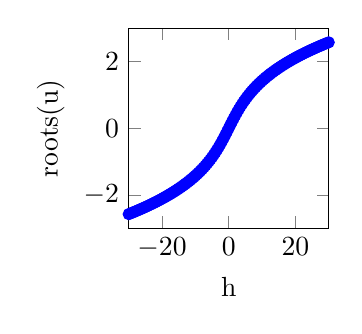
\begin{tikzpicture}

\begin{axis}[%
width=1in,
height=1in,
at={(0.758333in,0.48125in)},
scale only axis,
xmin=-30,
xmax=30,
xlabel={h},
ymin=-3,
ymax=3,
ylabel={roots(u)}
]
\addplot [color=blue,only marks,mark=*,mark options={solid},forget plot]
  table[row sep=crcr]{%
-30	-2.57705320212052\\
};
\addplot [color=blue,only marks,mark=*,mark options={solid},forget plot]
  table[row sep=crcr]{%
-29.5	-2.55686581901043\\
};
\addplot [color=blue,only marks,mark=*,mark options={solid},forget plot]
  table[row sep=crcr]{%
-29	-2.53642117566156\\
};
\addplot [color=blue,only marks,mark=*,mark options={solid},forget plot]
  table[row sep=crcr]{%
-28.5	-2.51571135876816\\
};
\addplot [color=blue,only marks,mark=*,mark options={solid},forget plot]
  table[row sep=crcr]{%
-28	-2.49472807146507\\
};
\addplot [color=blue,only marks,mark=*,mark options={solid},forget plot]
  table[row sep=crcr]{%
-27.5	-2.47346260798739\\
};
\addplot [color=blue,only marks,mark=*,mark options={solid},forget plot]
  table[row sep=crcr]{%
-27	-2.45190582621328\\
};
\addplot [color=blue,only marks,mark=*,mark options={solid},forget plot]
  table[row sep=crcr]{%
-26.5	-2.43004811787614\\
};
\addplot [color=blue,only marks,mark=*,mark options={solid},forget plot]
  table[row sep=crcr]{%
-26	-2.40787937620792\\
};
\addplot [color=blue,only marks,mark=*,mark options={solid},forget plot]
  table[row sep=crcr]{%
-25.5	-2.38538896074644\\
};
\addplot [color=blue,only marks,mark=*,mark options={solid},forget plot]
  table[row sep=crcr]{%
-25	-2.3625656590074\\
};
\addplot [color=blue,only marks,mark=*,mark options={solid},forget plot]
  table[row sep=crcr]{%
-24.5	-2.33939764468509\\
};
\addplot [color=blue,only marks,mark=*,mark options={solid},forget plot]
  table[row sep=crcr]{%
-24	-2.31587243200378\\
};
\addplot [color=blue,only marks,mark=*,mark options={solid},forget plot]
  table[row sep=crcr]{%
-23.5	-2.29197682579418\\
};
\addplot [color=blue,only marks,mark=*,mark options={solid},forget plot]
  table[row sep=crcr]{%
-23	-2.2676968668146\\
};
\addplot [color=blue,only marks,mark=*,mark options={solid},forget plot]
  table[row sep=crcr]{%
-22.5	-2.24301777177436\\
};
\addplot [color=blue,only marks,mark=*,mark options={solid},forget plot]
  table[row sep=crcr]{%
-22	-2.21792386744511\\
};
\addplot [color=blue,only marks,mark=*,mark options={solid},forget plot]
  table[row sep=crcr]{%
-21.5	-2.19239851816396\\
};
\addplot [color=blue,only marks,mark=*,mark options={solid},forget plot]
  table[row sep=crcr]{%
-21	-2.16642404593811\\
};
\addplot [color=blue,only marks,mark=*,mark options={solid},forget plot]
  table[row sep=crcr]{%
-20.5	-2.13998164225225\\
};
\addplot [color=blue,only marks,mark=*,mark options={solid},forget plot]
  table[row sep=crcr]{%
-20	-2.11305127055543\\
};
\addplot [color=blue,only marks,mark=*,mark options={solid},forget plot]
  table[row sep=crcr]{%
-19.5	-2.08561155826049\\
};
\addplot [color=blue,only marks,mark=*,mark options={solid},forget plot]
  table[row sep=crcr]{%
-19	-2.0576396769236\\
};
\addplot [color=blue,only marks,mark=*,mark options={solid},forget plot]
  table[row sep=crcr]{%
-18.5	-2.02911120908101\\
};
\addplot [color=blue,only marks,mark=*,mark options={solid},forget plot]
  table[row sep=crcr]{%
-18	-2\\
};
\addplot [color=blue,only marks,mark=*,mark options={solid},forget plot]
  table[row sep=crcr]{%
-17.5	-1.97027799234831\\
};
\addplot [color=blue,only marks,mark=*,mark options={solid},forget plot]
  table[row sep=crcr]{%
-17	-1.93991504149533\\
};
\addplot [color=blue,only marks,mark=*,mark options={solid},forget plot]
  table[row sep=crcr]{%
-16.5	-1.90887870882483\\
};
\addplot [color=blue,only marks,mark=*,mark options={solid},forget plot]
  table[row sep=crcr]{%
-16	-1.87713403005796\\
};
\addplot [color=blue,only marks,mark=*,mark options={solid},forget plot]
  table[row sep=crcr]{%
-15.5	-1.84464325515245\\
};
\addplot [color=blue,only marks,mark=*,mark options={solid},forget plot]
  table[row sep=crcr]{%
-15	-1.81136555585605\\
};
\addplot [color=blue,only marks,mark=*,mark options={solid},forget plot]
  table[row sep=crcr]{%
-14.5	-1.7772566964489\\
};
\addplot [color=blue,only marks,mark=*,mark options={solid},forget plot]
  table[row sep=crcr]{%
-14	-1.74226866261473\\
};
\addplot [color=blue,only marks,mark=*,mark options={solid},forget plot]
  table[row sep=crcr]{%
-13.5	-1.70634924274602\\
};
\addplot [color=blue,only marks,mark=*,mark options={solid},forget plot]
  table[row sep=crcr]{%
-13	-1.66944155533927\\
};
\addplot [color=blue,only marks,mark=*,mark options={solid},forget plot]
  table[row sep=crcr]{%
-12.5	-1.63148351551833\\
};
\addplot [color=blue,only marks,mark=*,mark options={solid},forget plot]
  table[row sep=crcr]{%
-12	-1.59240723321832\\
};
\addplot [color=blue,only marks,mark=*,mark options={solid},forget plot]
  table[row sep=crcr]{%
-11.5	-1.5521383353021\\
};
\addplot [color=blue,only marks,mark=*,mark options={solid},forget plot]
  table[row sep=crcr]{%
-11	-1.51059520408736\\
};
\addplot [color=blue,only marks,mark=*,mark options={solid},forget plot]
  table[row sep=crcr]{%
-10.5	-1.46768812578525\\
};
\addplot [color=blue,only marks,mark=*,mark options={solid},forget plot]
  table[row sep=crcr]{%
-10	-1.42331834475307\\
};
\addplot [color=blue,only marks,mark=*,mark options={solid},forget plot]
  table[row sep=crcr]{%
-9.5	-1.37737702412313\\
};
\addplot [color=blue,only marks,mark=*,mark options={solid},forget plot]
  table[row sep=crcr]{%
-9	-1.32974412166616\\
};
\addplot [color=blue,only marks,mark=*,mark options={solid},forget plot]
  table[row sep=crcr]{%
-8.5	-1.28028720381132\\
};
\addplot [color=blue,only marks,mark=*,mark options={solid},forget plot]
  table[row sep=crcr]{%
-8	-1.22886024384957\\
};
\addplot [color=blue,only marks,mark=*,mark options={solid},forget plot]
  table[row sep=crcr]{%
-7.5	-1.1753024874481\\
};
\addplot [color=blue,only marks,mark=*,mark options={solid},forget plot]
  table[row sep=crcr]{%
-7	-1.11943752706263\\
};
\addplot [color=blue,only marks,mark=*,mark options={solid},forget plot]
  table[row sep=crcr]{%
-6.5	-1.06107281726788\\
};
\addplot [color=blue,only marks,mark=*,mark options={solid},forget plot]
  table[row sep=crcr]{%
-6	-1\\
};
\addplot [color=blue,only marks,mark=*,mark options={solid},forget plot]
  table[row sep=crcr]{%
-5.5	-0.935996610506543\\
};
\addplot [color=blue,only marks,mark=*,mark options={solid},forget plot]
  table[row sep=crcr]{%
-5	-0.868830020341475\\
};
\addplot [color=blue,only marks,mark=*,mark options={solid},forget plot]
  table[row sep=crcr]{%
-4.5	-0.798264852522518\\
};
\addplot [color=blue,only marks,mark=*,mark options={solid},forget plot]
  table[row sep=crcr]{%
-4	-0.724075551386281\\
};
\addplot [color=blue,only marks,mark=*,mark options={solid},forget plot]
  table[row sep=crcr]{%
-3.5	-0.646066196249154\\
};
\addplot [color=blue,only marks,mark=*,mark options={solid},forget plot]
  table[row sep=crcr]{%
-3	-0.564099733027564\\
};
\addplot [color=blue,only marks,mark=*,mark options={solid},forget plot]
  table[row sep=crcr]{%
-2.5	-0.478138004979429\\
};
\addplot [color=blue,only marks,mark=*,mark options={solid},forget plot]
  table[row sep=crcr]{%
-2	-0.388291441004745\\
};
\addplot [color=blue,only marks,mark=*,mark options={solid},forget plot]
  table[row sep=crcr]{%
-1.5	-0.294872195425173\\
};
\addplot [color=blue,only marks,mark=*,mark options={solid},forget plot]
  table[row sep=crcr]{%
-1	-0.198437214538623\\
};
\addplot [color=blue,only marks,mark=*,mark options={solid},forget plot]
  table[row sep=crcr]{%
-0.5	-0.0998011904871354\\
};
\addplot [color=blue,only marks,mark=*,mark options={solid},forget plot]
  table[row sep=crcr]{%
0	0\\
};
\addplot [color=blue,only marks,mark=*,mark options={solid},forget plot]
  table[row sep=crcr]{%
0.5	0.0998011904871354\\
};
\addplot [color=blue,only marks,mark=*,mark options={solid},forget plot]
  table[row sep=crcr]{%
1	0.198437214538623\\
};
\addplot [color=blue,only marks,mark=*,mark options={solid},forget plot]
  table[row sep=crcr]{%
1.5	0.294872195425173\\
};
\addplot [color=blue,only marks,mark=*,mark options={solid},forget plot]
  table[row sep=crcr]{%
2	0.388291441004745\\
};
\addplot [color=blue,only marks,mark=*,mark options={solid},forget plot]
  table[row sep=crcr]{%
2.5	0.478138004979429\\
};
\addplot [color=blue,only marks,mark=*,mark options={solid},forget plot]
  table[row sep=crcr]{%
3	0.564099733027564\\
};
\addplot [color=blue,only marks,mark=*,mark options={solid},forget plot]
  table[row sep=crcr]{%
3.5	0.646066196249154\\
};
\addplot [color=blue,only marks,mark=*,mark options={solid},forget plot]
  table[row sep=crcr]{%
4	0.724075551386281\\
};
\addplot [color=blue,only marks,mark=*,mark options={solid},forget plot]
  table[row sep=crcr]{%
4.5	0.798264852522518\\
};
\addplot [color=blue,only marks,mark=*,mark options={solid},forget plot]
  table[row sep=crcr]{%
5	0.868830020341475\\
};
\addplot [color=blue,only marks,mark=*,mark options={solid},forget plot]
  table[row sep=crcr]{%
5.5	0.935996610506543\\
};
\addplot [color=blue,only marks,mark=*,mark options={solid},forget plot]
  table[row sep=crcr]{%
6	1\\
};
\addplot [color=blue,only marks,mark=*,mark options={solid},forget plot]
  table[row sep=crcr]{%
6.5	1.06107281726788\\
};
\addplot [color=blue,only marks,mark=*,mark options={solid},forget plot]
  table[row sep=crcr]{%
7	1.11943752706263\\
};
\addplot [color=blue,only marks,mark=*,mark options={solid},forget plot]
  table[row sep=crcr]{%
7.5	1.1753024874481\\
};
\addplot [color=blue,only marks,mark=*,mark options={solid},forget plot]
  table[row sep=crcr]{%
8	1.22886024384957\\
};
\addplot [color=blue,only marks,mark=*,mark options={solid},forget plot]
  table[row sep=crcr]{%
8.5	1.28028720381132\\
};
\addplot [color=blue,only marks,mark=*,mark options={solid},forget plot]
  table[row sep=crcr]{%
9	1.32974412166616\\
};
\addplot [color=blue,only marks,mark=*,mark options={solid},forget plot]
  table[row sep=crcr]{%
9.5	1.37737702412313\\
};
\addplot [color=blue,only marks,mark=*,mark options={solid},forget plot]
  table[row sep=crcr]{%
10	1.42331834475307\\
};
\addplot [color=blue,only marks,mark=*,mark options={solid},forget plot]
  table[row sep=crcr]{%
10.5	1.46768812578525\\
};
\addplot [color=blue,only marks,mark=*,mark options={solid},forget plot]
  table[row sep=crcr]{%
11	1.51059520408736\\
};
\addplot [color=blue,only marks,mark=*,mark options={solid},forget plot]
  table[row sep=crcr]{%
11.5	1.5521383353021\\
};
\addplot [color=blue,only marks,mark=*,mark options={solid},forget plot]
  table[row sep=crcr]{%
12	1.59240723321832\\
};
\addplot [color=blue,only marks,mark=*,mark options={solid},forget plot]
  table[row sep=crcr]{%
12.5	1.63148351551833\\
};
\addplot [color=blue,only marks,mark=*,mark options={solid},forget plot]
  table[row sep=crcr]{%
13	1.66944155533927\\
};
\addplot [color=blue,only marks,mark=*,mark options={solid},forget plot]
  table[row sep=crcr]{%
13.5	1.70634924274602\\
};
\addplot [color=blue,only marks,mark=*,mark options={solid},forget plot]
  table[row sep=crcr]{%
14	1.74226866261473\\
};
\addplot [color=blue,only marks,mark=*,mark options={solid},forget plot]
  table[row sep=crcr]{%
14.5	1.7772566964489\\
};
\addplot [color=blue,only marks,mark=*,mark options={solid},forget plot]
  table[row sep=crcr]{%
15	1.81136555585605\\
};
\addplot [color=blue,only marks,mark=*,mark options={solid},forget plot]
  table[row sep=crcr]{%
15.5	1.84464325515245\\
};
\addplot [color=blue,only marks,mark=*,mark options={solid},forget plot]
  table[row sep=crcr]{%
16	1.87713403005796\\
};
\addplot [color=blue,only marks,mark=*,mark options={solid},forget plot]
  table[row sep=crcr]{%
16.5	1.90887870882483\\
};
\addplot [color=blue,only marks,mark=*,mark options={solid},forget plot]
  table[row sep=crcr]{%
17	1.93991504149533\\
};
\addplot [color=blue,only marks,mark=*,mark options={solid},forget plot]
  table[row sep=crcr]{%
17.5	1.97027799234831\\
};
\addplot [color=blue,only marks,mark=*,mark options={solid},forget plot]
  table[row sep=crcr]{%
18	2\\
};
\addplot [color=blue,only marks,mark=*,mark options={solid},forget plot]
  table[row sep=crcr]{%
18.5	2.02911120908101\\
};
\addplot [color=blue,only marks,mark=*,mark options={solid},forget plot]
  table[row sep=crcr]{%
19	2.0576396769236\\
};
\addplot [color=blue,only marks,mark=*,mark options={solid},forget plot]
  table[row sep=crcr]{%
19.5	2.08561155826049\\
};
\addplot [color=blue,only marks,mark=*,mark options={solid},forget plot]
  table[row sep=crcr]{%
20	2.11305127055543\\
};
\addplot [color=blue,only marks,mark=*,mark options={solid},forget plot]
  table[row sep=crcr]{%
20.5	2.13998164225225\\
};
\addplot [color=blue,only marks,mark=*,mark options={solid},forget plot]
  table[row sep=crcr]{%
21	2.16642404593811\\
};
\addplot [color=blue,only marks,mark=*,mark options={solid},forget plot]
  table[row sep=crcr]{%
21.5	2.19239851816396\\
};
\addplot [color=blue,only marks,mark=*,mark options={solid},forget plot]
  table[row sep=crcr]{%
22	2.21792386744511\\
};
\addplot [color=blue,only marks,mark=*,mark options={solid},forget plot]
  table[row sep=crcr]{%
22.5	2.24301777177436\\
};
\addplot [color=blue,only marks,mark=*,mark options={solid},forget plot]
  table[row sep=crcr]{%
23	2.2676968668146\\
};
\addplot [color=blue,only marks,mark=*,mark options={solid},forget plot]
  table[row sep=crcr]{%
23.5	2.29197682579418\\
};
\addplot [color=blue,only marks,mark=*,mark options={solid},forget plot]
  table[row sep=crcr]{%
24	2.31587243200378\\
};
\addplot [color=blue,only marks,mark=*,mark options={solid},forget plot]
  table[row sep=crcr]{%
24.5	2.33939764468509\\
};
\addplot [color=blue,only marks,mark=*,mark options={solid},forget plot]
  table[row sep=crcr]{%
25	2.3625656590074\\
};
\addplot [color=blue,only marks,mark=*,mark options={solid},forget plot]
  table[row sep=crcr]{%
25.5	2.38538896074644\\
};
\addplot [color=blue,only marks,mark=*,mark options={solid},forget plot]
  table[row sep=crcr]{%
26	2.40787937620792\\
};
\addplot [color=blue,only marks,mark=*,mark options={solid},forget plot]
  table[row sep=crcr]{%
26.5	2.43004811787614\\
};
\addplot [color=blue,only marks,mark=*,mark options={solid},forget plot]
  table[row sep=crcr]{%
27	2.45190582621328\\
};
\addplot [color=blue,only marks,mark=*,mark options={solid},forget plot]
  table[row sep=crcr]{%
27.5	2.47346260798739\\
};
\addplot [color=blue,only marks,mark=*,mark options={solid},forget plot]
  table[row sep=crcr]{%
28	2.49472807146507\\
};
\addplot [color=blue,only marks,mark=*,mark options={solid},forget plot]
  table[row sep=crcr]{%
28.5	2.51571135876816\\
};
\addplot [color=blue,only marks,mark=*,mark options={solid},forget plot]
  table[row sep=crcr]{%
29	2.53642117566156\\
};
\addplot [color=blue,only marks,mark=*,mark options={solid},forget plot]
  table[row sep=crcr]{%
29.5	2.55686581901043\\
};
\addplot [color=blue,only marks,mark=*,mark options={solid},forget plot]
  table[row sep=crcr]{%
30	2.57705320212052\\
};
\end{axis}
\end{tikzpicture}%
\end{document}
\caption{Solution branches with the function $-\frac{1}{2} u^3 + ru $ numerous colors for different $r\in [-30,30]$ and the constant function $h=-5$ in red (left). Root locus plot for the same $r$ values (right).}
\label{fig:tree}
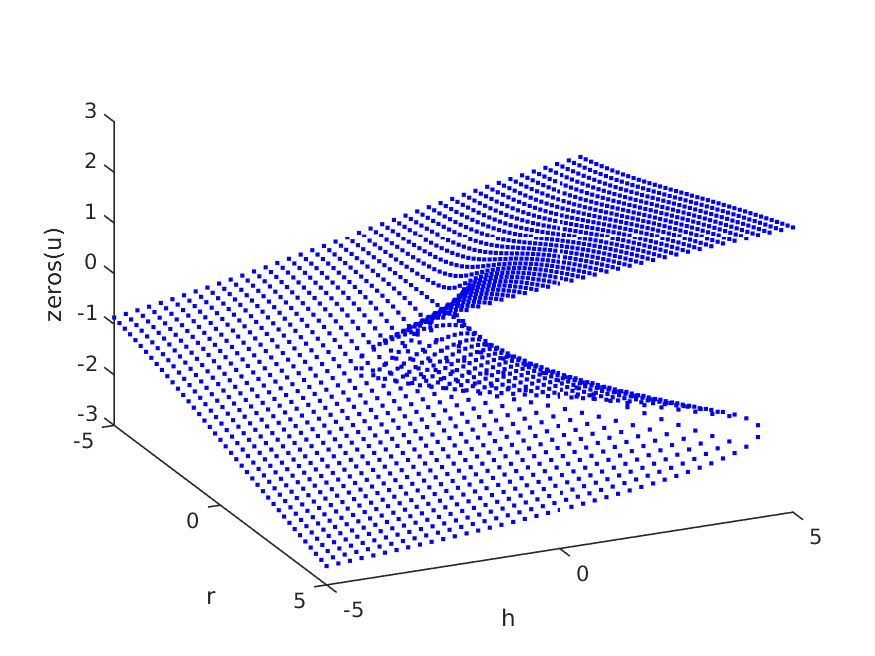
\includegraphics[scale = 0.5]{./plots/zerosrhu.pdf}
\caption{$r,h,u$ plot of the polynomial roots.}
\end{figure}

\newpage
\subsection{\texttt{matcont} analysis}
\begin{figure}
% This file was created by matlab2tikz.
% Minimal pgfplots version: 1.3
%
%The latest updates can be retrieved from
%  http://www.mathworks.com/matlabcentral/fileexchange/22022-matlab2tikz
%where you can also make suggestions and rate matlab2tikz.
%
\documentclass[tikz]{standalone}
\usepackage{pgfplots}
\usepackage{grffile}
\pgfplotsset{compat=newest}
\usetikzlibrary{plotmarks}
\usepackage{amsmath}

\begin{document}
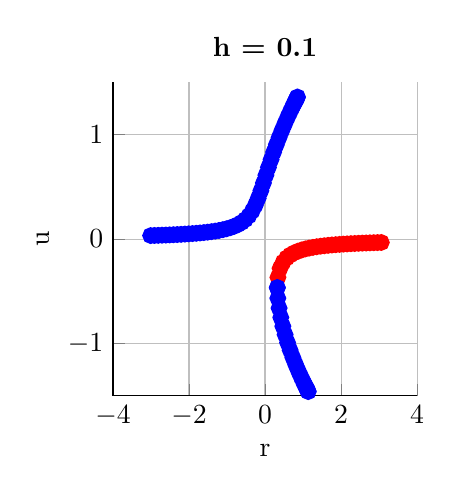
\begin{tikzpicture}

\begin{axis}[%
width=1.520833in,
height=1.565625in,
at={(0.758333in,0.48125in)},
scale only axis,
xmin=-4,
xmax=4,
xlabel={r},
xmajorgrids,
ymin=-1.5,
ymax=1.5,
ylabel={u},
ymajorgrids,
title style={font=\bfseries},
title={h = 0.1},
axis x line*=bottom,
axis y line*=left
]
\addplot [color=red,line width=2.0pt,only marks,mark=*,mark options={solid},forget plot]
  table[row sep=crcr]{%
0.339884584905381	-0.366838979220343\\
0.395445783870946	-0.280905268665007\\
0.477039677221064	-0.220928583373488\\
0.569131781763994	-0.18090772964447\\
0.665301287607463	-0.152999510457211\\
0.763240458800295	-0.132545787398467\\
0.86203673857466	-0.116931680482687\\
0.961287168341235	-0.104622844217296\\
1.06079613500985	-0.0946687258560345\\
1.16046102349105	-0.0864510363154362\\
1.26022448414282	-0.0795506768357676\\
1.36005274565222	-0.073673571001199\\
1.45992503288788	-0.0686072664488551\\
1.55982808358445	-0.0641944270951588\\
1.65975315842395	-0.0603160265365267\\
1.75969433789576	-0.0568803413247673\\
1.85964751476849	-0.053815536069618\\
1.95960977806716	-0.0510645429273886\\
2.05957902532009	-0.0485814473210156\\
2.15955371211596	-0.0463288867540137\\
2.25953268657988	-0.0442761459329365\\
2.35951507768718	-0.0423977398421841\\
2.45950021848172	-0.0406723447920934\\
2.55948759238611	-0.0390819815778706\\
2.65947679507292	-0.0376113839466004\\
2.75946750699976	-0.0362475050754164\\
2.85945947336581	-0.0349791280842977\\
2.95945248930727	-0.0337965558480406\\
3.05944638883975	-0.0326913618767811\\
};
\addplot [color=blue,line width=2.0pt,only marks,mark=*,mark options={solid},forget plot]
  table[row sep=crcr]{%
0.853109651581944	1.3613\\
0.844947784468234	1.3555221107821\\
0.834352767925008	1.34798912650505\\
0.820605599630924	1.33815927268243\\
0.802779506448533	1.32531741771648\\
0.779683556697022	1.30851522940011\\
0.74979405399666	1.28648753071671\\
0.711174059345345	1.25753316075611\\
0.661385271341851	1.21934142524044\\
0.597405442637901	1.1687328169283\\
0.52020564297685	1.10516081369604\\
0.444472906859391	1.03984700803666\\
0.370317062526629	0.972747327313107\\
0.297831083256804	0.903846588648476\\
0.227069043444074	0.833176593753761\\
0.158008702056026	0.76084388588675\\
0.0904896443412382	0.687072925210984\\
0.0241147295551347	0.612274653914456\\
-0.0418960169496728	0.537157535002335\\
-0.108886146459887	0.462905409446389\\
-0.178868279177768	0.391426665592857\\
-0.254215194528591	0.325523117392324\\
-0.336531039123596	0.268416856547319\\
-0.425422571414595	0.222171534175945\\
-0.518976742012909	0.18644290798753\\
-0.615291018768352	0.159243220078257\\
-0.713130809394272	0.138369266860577\\
-0.811813589255917	0.122060921975311\\
-0.910976169403683	0.109060381058396\\
-1.01042266879132	0.0984956400256325\\
-1.11004394344915	0.0897607697982959\\
-1.20977683823806	0.0824284027818385\\
-1.30958341980079	0.0761912902767676\\
-1.40944009893196	0.0708241315901732\\
-1.50933173673661	0.0661585594802886\\
-1.60924833838221	0.0620665248633288\\
-1.70918313564016	0.0584490674711001\\
-1.80913143986024	0.0552285858139589\\
-1.90908993601179	0.0523434187092996\\
-2.00905623675065	0.0497439809477482\\
-2.1090285939876	0.0473899623239459\\
-2.2090057082594	0.0452482666062612\\
-2.30898660023265	0.0432914736688389\\
-2.40897052251402	0.0414966770916752\\
-2.50895689811512	0.0398445950187067\\
-2.60894527685875	0.0383188824905429\\
-2.70893530405969	0.0369055941344918\\
-2.80892669773106	0.0355927603354159\\
-2.90891923179517	0.0343700499592586\\
-3.00891272357859	0.0332284997406959\\
1.13683843105486	-1.4618\\
1.1286778691202	-1.45602026521672\\
1.11808702307842	-1.44848141337766\\
1.10434964888071	-1.43863786467882\\
1.08654412076311	-1.42576748259288\\
1.06348918382842	-1.4089089954837\\
1.03367962298857	-1.38677306832192\\
0.995214695289403	-1.3576125955399\\
0.945729626591977	-1.31902704281401\\
0.882359369866967	-1.26765413194907\\
0.806345587069925	-1.20266090831589\\
0.732472161718774	-1.13524012517769\\
0.661137978063838	-1.06513180777353\\
0.592865114961316	-0.992029945405816\\
0.528357226027812	-0.915571803093406\\
0.468598529697682	-0.835326037652483\\
0.415032905896466	-0.750784867610669\\
0.369912489614977	-0.661383995823696\\
0.337023103958351	-0.566654756753944\\
0.323177120682036	-0.466983232540273\\
0.323165203506072	-0.464159810396268\\
};
\end{axis}
\end{tikzpicture}%
\end{document}
% This file was created by matlab2tikz.
% Minimal pgfplots version: 1.3
%
%The latest updates can be retrieved from
%  http://www.mathworks.com/matlabcentral/fileexchange/22022-matlab2tikz
%where you can also make suggestions and rate matlab2tikz.
%
\documentclass[tikz]{standalone}
\usepackage{pgfplots}
\usepackage{grffile}
\pgfplotsset{compat=newest}
\usetikzlibrary{plotmarks}
\usepackage{amsmath}

\begin{document}
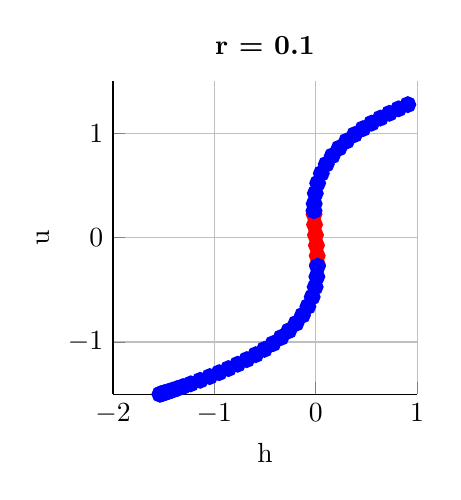
\begin{tikzpicture}

\begin{axis}[%
width=1.520833in,
height=1.565625in,
at={(0.758333in,0.48125in)},
scale only axis,
xmin=-2,
xmax=1,
xlabel={h},
xmajorgrids,
ymin=-1.5,
ymax=1.5,
ylabel={u},
ymajorgrids,
title style={font=\bfseries},
title={r = 0.1},
axis x line*=bottom,
axis y line*=left
]
\addplot [color=red,line width=2.0pt,only marks,mark=*,mark options={solid},forget plot]
  table[row sep=crcr]{%
0.0172132593164403	-0.258198580173871\\
0.0147402209112225	-0.173529013960578\\
0.00717842274835561	-0.0737934268906806\\
-0.00256474131123581	0.0257326095618084\\
-0.0115488389932111	0.125332044853498\\
-0.0168100032777963	0.22522160445782\\
};
\addplot [color=blue,line width=2.0pt,only marks,mark=*,mark options={solid},forget plot]
  table[row sep=crcr]{%
-1.5375	-1.5\\
-1.52793755915683	-1.49707429380943\\
-1.51551134658092	-1.49325469526034\\
-1.49936579709179	-1.48826154979844\\
-1.47839131736224	-1.48172297977811\\
-1.4511501335755	-1.47314096306555\\
-1.41578162680381	-1.46184225190658\\
-1.36988264972424	-1.44690522577578\\
-1.31035881072511	-1.42704673037727\\
-1.23324588139307	-1.40043854849791\\
-1.13918014318183	-1.36649341565013\\
-1.04571096371212	-1.33093630499186\\
-0.952945396198833	-1.29357911059881\\
-0.861018479920045	-1.25419960959774\\
-0.770102868076978	-1.21253355420546\\
-0.680422505461459	-1.16826489080988\\
-0.592272277837111	-1.12101400422773\\
-0.506046435610702	-1.07032446077076\\
-0.42227963177681	-1.01565022905008\\
-0.341705007530768	-0.956348905142977\\
-0.265331735529844	-0.891694069586142\\
-0.19453361623281	-0.820933901665853\\
-0.131107467379937	-0.743440954289538\\
-0.0771920624946128	-0.658993603720877\\
-0.0348759179508299	-0.568132019659551\\
-0.00544996332266926	-0.472311179412507\\
0.0112952768153624	-0.373524508722048\\
0.0171199888444952	-0.273565695222044\\
-0.0172132593164711	0.258199017795372\\
-0.0153191938196579	0.325285841068316\\
-0.00415095434620807	0.424802315150452\\
0.019009579549844	0.522295367020695\\
0.0551717284487706	0.615785239558364\\
0.103716637719419	0.703470815629188\\
0.162833561208178	0.784350693632782\\
0.230329685821229	0.858313870324109\\
0.304214948617562	0.925834365901177\\
0.382912648302724	0.987631518105198\\
0.465248413644104	1.0444570282561\\
0.550366964976863	1.09699831593158\\
0.63764659860519	1.14584838885145\\
0.726631594982482	1.19150583983007\\
0.81698348903627	1.23438585609745\\
0.908447115910144	1.27483370328393\\
};
\end{axis}
\end{tikzpicture}%
\end{document}
\end{figure}

\begin{figure}
% This file was created by matlab2tikz.
% Minimal pgfplots version: 1.3
%
%The latest updates can be retrieved from
%  http://www.mathworks.com/matlabcentral/fileexchange/22022-matlab2tikz
%where you can also make suggestions and rate matlab2tikz.
%
\documentclass[tikz]{standalone}
\usepackage{pgfplots}
\usepackage{grffile}
\pgfplotsset{compat=newest}
\usetikzlibrary{plotmarks}
\usepackage{amsmath}

\begin{document}
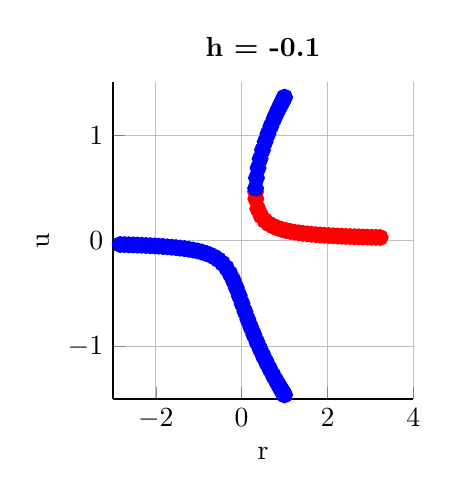
\begin{tikzpicture}

\begin{axis}[%
width=1.501562in,
height=1.582604in,
at={(0.771875in,0.483542in)},
scale only axis,
xmin=-3,
xmax=4,
xlabel={r},
xmajorgrids,
ymin=-1.5,
ymax=1.5,
ylabel={u},
ymajorgrids,
title style={font=\bfseries},
title={h = -0.1},
axis x line*=bottom,
axis y line*=left
]
\addplot [color=red,line width=2.0pt,only marks,mark=*,mark options={solid},forget plot]
  table[row sep=crcr]{%
0.323165203505057	0.464158456001476\\
0.330804018837246	0.396537225812541\\
0.374937685100872	0.304280184949715\\
0.450747998588276	0.236532948872617\\
0.540662760369767	0.191447390821352\\
0.635950570565475	0.160495301423005\\
0.733488453005002	0.138131408867153\\
0.832082625524427	0.121251560279991\\
0.931222615403565	0.108063272956082\\
1.03066715971252	0.097473811410388\\
1.13029242657983	0.0887822489601224\\
1.23003043394259	0.0815190082703909\\
1.32984173785293	0.075357817519983\\
1.42970237357581	0.0700649166084488\\
1.52959720382557	0.0654684136877241\\
1.62951634423686	0.0614390639103868\\
1.72945315258916	0.0578777982615054\\
1.82940305216934	0.0547073903238861\\
1.92936281917876	0.0518667426870119\\
2.02933013795445	0.0493068795419564\\
2.12930331583733	0.0469880788072688\\
2.22928109598018	0.0448777825516222\\
2.3292625318014	0.0429490497490124\\
2.42924690114507	0.0411793938180787\\
2.52923364655487	0.0395498976540019\\
2.6292223330508	0.0380445317657171\\
2.72921261784129	0.0366496230960698\\
2.82920422830433	0.0353534370266159\\
2.92919694578127	0.0341458453745479\\
3.02919059351213	0.03301806041259\\
3.12918502755831	0.0319624200755683\\
3.2291801299056	0.030972213211333\\
};
\addplot [color=blue,line width=2.0pt,only marks,mark=*,mark options={solid},forget plot]
  table[row sep=crcr]{%
1.00002803841806	1.3613\\
0.992092634108343	1.35521481258046\\
0.9817989198664	1.34727504695192\\
0.968455492756058	1.33690372966119\\
0.951175512176068	1.32333586524918\\
0.928827489580958	1.30555081620623\\
0.899979398490617	1.2821754580726\\
0.862842017451248	1.25134150562155\\
0.815228503994606	1.21046750929859\\
0.754575412208822	1.15590955829722\\
0.682424411250749	1.08664435973167\\
0.613160859219861	1.01448365876912\\
0.547425399953479	0.939083120451077\\
0.486103254499327	0.860033366824615\\
0.430472797775995	0.776849766740561\\
0.382488298494675	0.688978921603085\\
0.345358123841503	0.595888313853771\\
0.324761828129712	0.497539327943608\\
1.00002080894514	-1.4618\\
0.991690088942846	-1.45626834863637\\
0.980873315308752	-1.4490574132348\\
0.966834013526776	-1.43964951588283\\
0.948621532067838	-1.42736180003297\\
0.925011856971095	-1.41128951007417\\
0.894434678005757	-1.39022687609414\\
0.854886019046957	-1.3625546384335\\
0.803828830065245	-1.32607636906833\\
0.738091522363492	-1.27777357155456\\
0.658560985028314	-1.21714460244475\\
0.580296202035428	-1.15488925119707\\
0.503409476478917	-1.09093872693547\\
0.428014679161863	-1.02523490150405\\
0.35421927101714	-0.957738864076055\\
0.282109981948082	-0.888443946633087\\
0.211727990779998	-0.817395589584608\\
0.143027030642908	-0.744721888059375\\
0.0758045873353195	-0.670681301383195\\
0.0095935472327065	-0.595738787110011\\
-0.05649438134147	-0.520689363186512\\
-0.123948090667498	-0.446853367771375\\
-0.194910468595783	-0.376331504355512\\
-0.271710758769771	-0.312097132508936\\
-0.355583115475566	-0.25728111841533\\
-0.445685720898715	-0.213461469265637\\
-0.539989332975677	-0.179806163533463\\
-0.636722049173044	-0.154176507400238\\
-0.73479161816279	-0.134439570729968\\
-0.833603562301397	-0.118951565687894\\
-0.932841515964072	-0.106550958137818\\
-1.03233378938098	-0.0964335492989013\\
-1.1319839353514	-0.0880390673735213\\
-1.23173567708791	-0.0809707545670417\\
-1.33155494455765	-0.0749421200290592\\
-1.43142039753934	-0.0697421862439138\\
-1.53131825115002	-0.0652126592769646\\
-1.63123935131179	-0.0612327097115901\\
-1.73117746670247	-0.0577086455450828\\
-1.83112826035573	-0.0545667744748916\\
-1.93108865295107	-0.0517483811439469\\
-2.0310564184449	-0.0492061318833773\\
-2.13102992123234	-0.046901459868207\\
-2.23100794165186	-0.0448026349457353\\
-2.33098955788038	-0.0428833191890342\\
-2.43097406457014	-0.0411214721524738\\
-2.53096091588053	-0.0394985113831793\\
-2.6309496849912	-0.0379986616502311\\
-2.73094003492948	-0.0366084453703666\\
-2.83093169728121	-0.0353162798538153\\
};
\end{axis}
\end{tikzpicture}%
\end{document}
% This file was created by matlab2tikz.
% Minimal pgfplots version: 1.3
%
%The latest updates can be retrieved from
%  http://www.mathworks.com/matlabcentral/fileexchange/22022-matlab2tikz
%where you can also make suggestions and rate matlab2tikz.
%
\documentclass[tikz]{standalone}
\usepackage{pgfplots}
\usepackage{grffile}
\pgfplotsset{compat=newest}
\usetikzlibrary{plotmarks}
\usepackage{amsmath}

\begin{document}
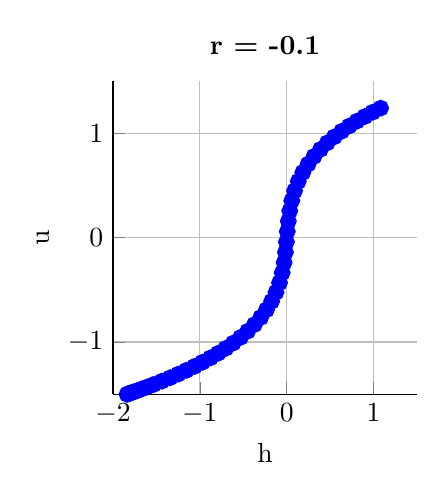
\begin{tikzpicture}

\begin{axis}[%
width=1.520833in,
height=1.565625in,
at={(0.758333in,0.48125in)},
scale only axis,
xmin=-2,
xmax=1.5,
xlabel={h},
xmajorgrids,
ymin=-1.5,
ymax=1.5,
ylabel={u},
ymajorgrids,
title style={font=\bfseries},
title={r = -0.1},
axis x line*=bottom,
axis y line*=left
]
\addplot [color=blue,line width=2.0pt,only marks,mark=*,mark options={solid},forget plot]
  table[row sep=crcr]{%
-1.8375	-1.5\\
-1.82789131529289	-1.49722994567433\\
-1.81540400845501	-1.49361508272609\\
-1.7991773441803	-1.48889220647889\\
-1.77809446270554	-1.48271211112278\\
-1.75070715382075	-1.47460854849244\\
-1.71513939444731	-1.46395376023031\\
-1.66896450622242	-1.44989304075143\\
-1.60905056400957	-1.43124512214104\\
-1.53137010548944	-1.40634390239235\\
-1.4364981829811	-1.37472524633303\\
-1.34207298004771	-1.34179512450297\\
-1.24816303984149	-1.30742141725568\\
-1.15485206734904	-1.27145138741715\\
-1.06224330951855	-1.23370752449022\\
-0.970465476962079	-1.19398248094997\\
-0.879680828278954	-1.15203296687782\\
-0.79009629151136	-1.10757256254888\\
-0.701978830491734	-1.06026364957988\\
-0.615676634394865	-1.00970923308952\\
-0.531647938098341	-0.955446660771038\\
-0.4504988122563	-0.896947718099618\\
-0.373028650078894	-0.833634079452886\\
-0.300274176301953	-0.764923921060951\\
-0.233524639491586	-0.690331665689541\\
-0.174250811465709	-0.60963563019007\\
-0.123869798255393	-0.523082226113022\\
-0.0833228462483304	-0.431504925790636\\
-0.0526200732772569	-0.3361987249375\\
-0.0306431185721461	-0.238553470440991\\
-0.0153316717935119	-0.139688186966303\\
-0.00406402452779214	-0.0403126820928591\\
0.00602136892567758	0.0591774982739514\\
0.0178390162368105	0.158486039549143\\
0.0342219055209436	0.257173791976155\\
0.0577132301234752	0.354459021457595\\
0.090223227749249	0.449158514131794\\
0.132663324008949	0.53987218231621\\
0.18482282274066	0.625367939203937\\
0.245632164093853	0.704918211220769\\
0.313634431611039	0.778375812077062\\
0.387379390427221	0.846026859415528\\
0.465623046058245	0.90838616628016\\
0.547376128419934	0.966041192612284\\
0.631879667650825	1.0195636374573\\
0.718559121998381	1.0694702019819\\
0.806979909751939	1.11621105099069\\
0.896811328177171	1.16017148650179\\
0.987799316214972	1.20167886742321\\
1.07974651328341	1.24101089263033\\
};
\end{axis}
\end{tikzpicture}%
\end{document}
\caption{\texttt{matcont output for $h=0.1$}}
\end{figure}

\begin{figure}
% This file was created by matlab2tikz.
% Minimal pgfplots version: 1.3
%
%The latest updates can be retrieved from
%  http://www.mathworks.com/matlabcentral/fileexchange/22022-matlab2tikz
%where you can also make suggestions and rate matlab2tikz.
%
\documentclass[tikz]{standalone}
\usepackage{pgfplots}
\usepackage{grffile}
\pgfplotsset{compat=newest}
\usetikzlibrary{plotmarks}
\usepackage{amsmath}

\begin{document}
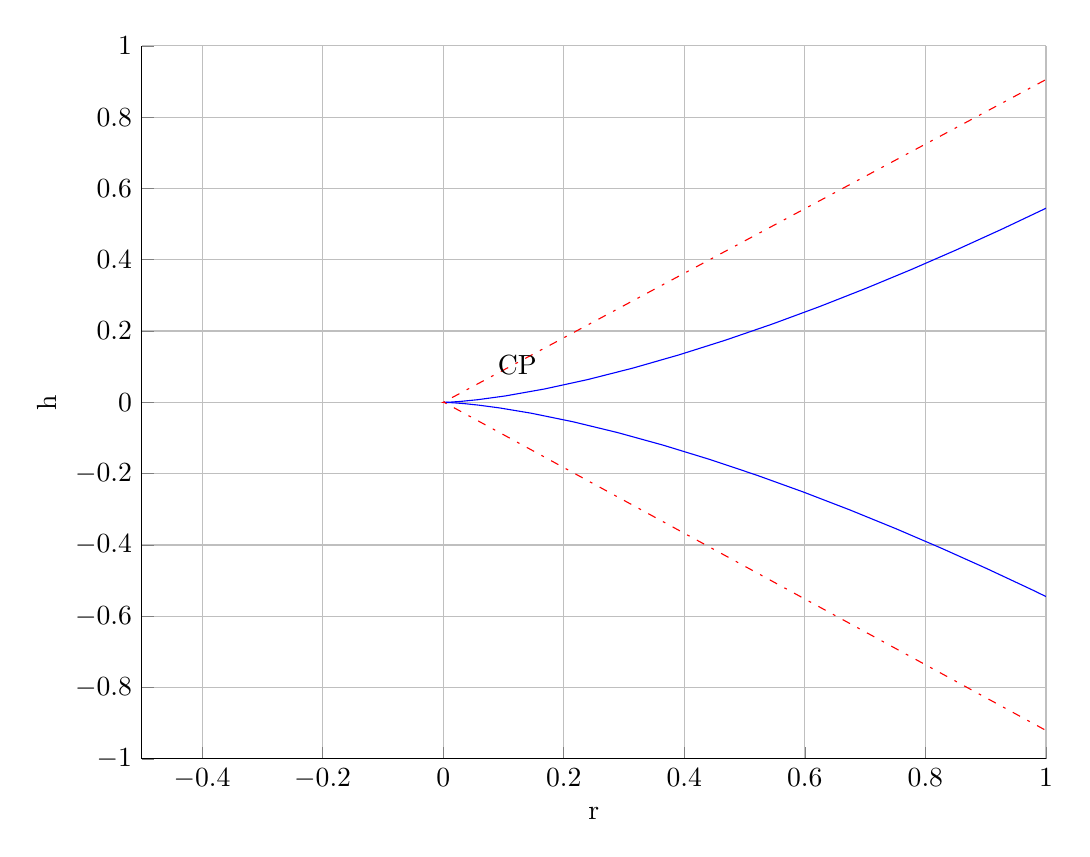
\begin{tikzpicture}

\begin{axis}[%
width=4.520833in,
height=3.565625in,
at={(0.758333in,0.48125in)},
scale only axis,
xmin=-0.5,
xmax=1,
xlabel={r},
xmajorgrids,
ymin=-1,
ymax=1,
ylabel={h},
ymajorgrids,
axis x line*=bottom,
axis y line*=left
]
\addplot [color=blue,solid,forget plot]
  table[row sep=crcr]{%
0.00165619984252548	-3.66886912457335e-05\\
0.000811760585048672	-1.25894005729519e-05\\
0.000158428756549472	-1.08546078378942e-06\\
5.00000003965211e-11	-2.91882927309295e-22\\
6.58968342926398e-05	2.91178919013112e-07\\
0.00122516888281572	2.33430203408821e-05\\
0.00486205060217964	0.000184540770656349\\
0.0130295386347732	0.000809574310461118\\
0.0289168829030127	0.00267664223181863\\
0.0570042319053886	0.00740838866759672\\
0.102866943704598	0.0179587814934319\\
0.168457324264403	0.0376355232709435\\
0.240029852031831	0.0640119411840362\\
0.314883492491183	0.0961807040833751\\
0.391435873864666	0.133307335724722\\
0.468739521794378	0.174686953279892\\
0.546213977736904	0.219739092136701\\
0.623497360485384	0.267987810411728\\
0.700361956752589	0.319041319325803\\
0.776664665991163	0.37257476206576\\
0.852316981335097	0.428316518099236\\
0.927266276032154	0.486037534398542\\
1.00148383881272	0.545543053161069\\
1.07495705504646	0.606666177729997\\
1.14768419608184	0.669262842461938\\
1.21967089545082	0.733207843767828\\
1.29092772997942	0.798391686825653\\
1.36146854331705	0.864718058274885\\
1.4313092731843	0.932101783494891\\
1.50046712659285	1.00046716303053\\
1.56895999776994	1.06974660746933\\
1.63680605722706	1.13987950923553\\
1.70402346289804	1.21081130423886\\
1.77063015781489	1.28249268551515\\
1.83664373159806	1.35487894178373\\
1.90208132671233	1.42792939647487\\
1.96695957829443	1.50160693059378\\
2.0312945775275	1.57587757395602\\
2.09510185271759	1.65071015403991\\
2.15839636275477	1.7260759925332\\
2.22119249978881	1.80194864238568\\
2.28350409805113	1.87830365859367\\
2.3453444472349	1.95511839797919\\
2.4067263087829	2.03237184344981\\
2.46766193429149	2.11004444953568\\
2.52816308482986	2.1881180057237\\
2.58824105105361	2.26657551567952\\
2.6479066731875	2.34540108962103\\
2.70717036110877	2.42457984876071\\
2.7660421138334	2.50409783968974\\
};
\addplot [color=red,dash pattern=on 1pt off 3pt on 3pt off 3pt,forget plot]
  table[row sep=crcr]{%
0.00165619984252548	-3.66886912457335e-05\\
5.00000003965211e-11	-2.91882927309295e-22\\
2.7660421138334	2.50409783968974\\
};
\node[right, align=left, inner sep=0mm, text=black]
at (axis cs:0.09000000005,0.105,0) {CP};
\addplot [color=blue,solid,forget plot]
  table[row sep=crcr]{%
0.00165619984252548	-3.66886912457335e-05\\
0.00279475789085515	-8.04228386263609e-05\\
0.00470818569431031	-0.00017585045110085\\
0.00791102464113478	-0.000383011856538927\\
0.0132378950824948	-0.000829070605359806\\
0.022008427422133	-0.00177724231545873\\
0.0362297658799251	-0.00375371592468311\\
0.0587911226103685	-0.00775944646317118\\
0.0935663159571612	-0.0155791014898593\\
0.145352886815526	-0.0301646717572165\\
0.215274769918436	-0.0543691836346927\\
0.289235766918821	-0.0846722512115947\\
0.365342642935137	-0.120202544390285\\
0.442470904886691	-0.160210209813507\\
0.51993669838624	-0.204074536841762\\
0.597315858152205	-0.251286512454427\\
0.67434203677627	-0.301427909390212\\
0.750847549891486	-0.354152868151616\\
0.82672791167475	-0.409173041132438\\
0.90191993333815	-0.466245968363931\\
0.976387834475514	-0.525166059639326\\
1.05011422959016	-0.585757592955285\\
1.12309416215597	-0.647869248391081\\
1.19533108492821	-0.711369813041771\\
1.2668341169443	-0.776144774156909\\
1.33761614630132	-0.842093597118219\\
1.40769250756638	-0.909127531930627\\
1.47708005264709	-0.977167830980674\\
1.54579649609306	-1.0461442906878\\
1.61385995235329	-1.11599404865666\\
1.68128861004234	-1.18666058555237\\
1.74810050331484	-1.25809289064992\\
1.8143133542544	-1.33024476114624\\
1.87994446522622	-1.40307420899028\\
1.94501064854798	-1.4765429571457\\
2.00952818285618	-1.55061600920987\\
2.07351278867835	-1.62526127973898\\
2.1369796182297	-1.70044927564508\\
2.19994325517933	-1.77615282013143\\
2.26241772173168	-1.85234681277446\\
2.32441649058977	-1.92900801991945\\
2.38595250045057	-2.00611489113654\\
2.44703817378361	-2.08364739789062\\
2.50768543584163	-2.16158689104672\\
2.56790573460529	-2.23991597501161\\
2.62771006081744	-2.3186183958168\\
2.68710896819791	-2.3976789418282\\
2.74611259294782	-2.47708335464326\\
2.80473067313081	-2.55681824981855\\
2.86297256719935	-2.63687104545742\\
};
\addplot [color=red,dash pattern=on 1pt off 3pt on 3pt off 3pt,forget plot]
  table[row sep=crcr]{%
0.00165619984252548	-3.66886912457335e-05\\
2.86297256719935	-2.63687104545742\\
};
\end{axis}
\end{tikzpicture}%
\end{document}
\end{figure}

\begin{figure}
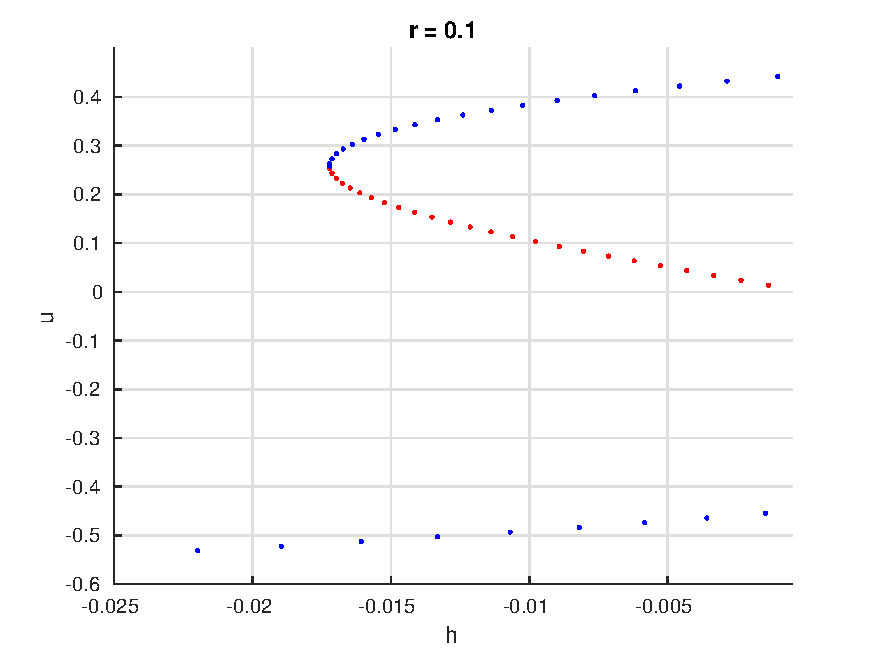
\includegraphics[scale = 1]{./plots/lastExercise.pdf}
\caption{Solution branch of $h \in [-0.0025,-0.0005].$ With \texttt{ opt=contset(opt,'MinStepsize',0.001);
 opt=contset(opt,'MaxStepsize',0.01); 
 opt=contset(opt,'MaxNewtonIters',4);}}
\end{figure}



\end{document}